\documentclass{computing}

\title{Theory of Computation}
\author{Jim Hef{}feron}

% \usepackage{layouts}
\usepackage{endnotes}

\includeonly{%
cover/cover,%
preface/preface,%
prologue/prologue,%
background/background,%
automata/automata,%
languages/languages,%
complexity/complexity%
}

\begin{document} % \setuplayouts

\thispagestyle{empty}
\setlength{\unitlength}{1in}
\noindent\begin{picture}(0,0)(1,-1)
  \put(4.25,-7.25){\hspace*{-0.5in}\makebox[0em]{\LARGE The Theory of Computation}}
  \put(4.25,-7.65){\hspace{-0.5in}\makebox[0em]{\Large Jim Hef{}feron}}
  \put(4.25,-6.25){\hspace*{-0.67in}\makebox[0em]{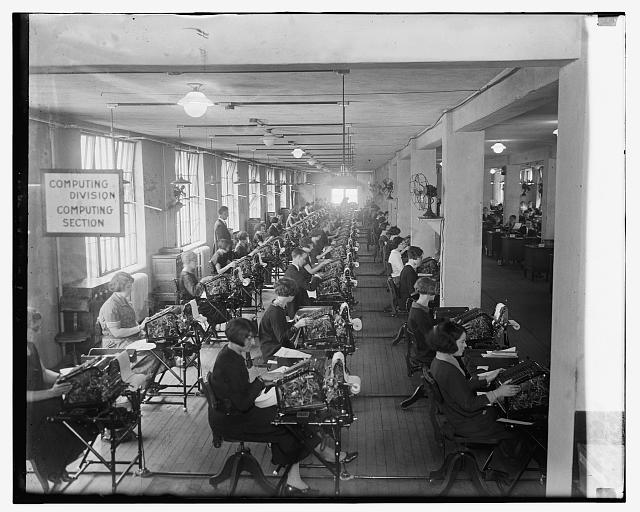
\includegraphics[width=\paperwidth]{cover/computingdivision.jpg}}}
\end{picture}


\titlepage
\frontmatter
\addtoendnotes{\citechapterformatting{Preface}}
\newcommand{\aphorism}[3]{%
  \vspace{3ex plus 1ex minus .2ex}%
  \noindent\parbox{.85\textwidth}{\raggedright\itshape #1 \\ 
    \hspace*{\fill}{\upshape -- #2, \MakeUppercase{#3}}}}

\newcommand{\header}[1]{\vspace{1ex}\par\noindent\textbf{#1}\hspace{0.618em plus 0.1em minus 0.05em}}


\chapter*{Preface}
The Theory of Computation is awfully nice.
It is beautiful, timely,
and has deep connections to other areas inside of computing,
to mathematics, and to the wider intellectual world.

The subject makes a delightful course.
Students learn both of the power of comptuation, and
of its limits.
There are underlying principles, but there are also as-yet
undiscovered areas within easy reach of a first course.
This text aims to mirror that, to be both rigorous and delightful.

We cover the standard curriculum, but in a way that is different
from standard texts, emphasizing intuition and background, as well
as arranging the material to make it possible to express to students
the current research frontier.




\header{For students}
The Theory of Computation has nearly a hundred year history.
The subject tells a story, from the initial settling on a precise definition,
through unsolvability results and a branching into areas such 
as automata, up to today's interest in complexity.

Here you will see that story, not in its full detail of course, but in
sufficient depth that you can understand both its main ideas and how
it applies to various other areas.

A liberal approach to education, according to a 
\citetext{favorite definition of mine}{\protect\url{https://www.aacu.org/leap/what-is-a-liberal-education}},
``empowers individuals and prepares them to deal with complexity, diversity, and change. This approach emphasizes broad knowledge \ldots{} as well as in-depth achievement in a specific field of interest.'' 
% https://www.aacu.org/leap/what-is-a-liberal-education
Here you will see the story told in a liberal way, but without stinting
on needed technical detail.




\header{For teachers}
This text covers the standard topics: Turing machines, unsolvability, 
automata, languages, and complexity.
But the approach of this book differs from the standard one 
in a number of ways,
all of which aim to bring out how awfully nice the subject is.

First, we start with Turing machines.
These are after all the touchstone.
We give a rigorous definition, but we also have an extensive discussion
of the motivation for that definition.
And, we also include an extensive discussion of Church's Thesis, 
taking care to include discussion of those point that experience with
questions on the Internet shows are points of frequent confusion. 

This approach illustrates the overall 
liberal program of not being shy about stopping, where stopping makes sense, 
to consider an interesting point, for its pure interest.

\citetext{Winklmann and Schauble}{\autocite{WinklmannSchauble}} 
use many familiar 
constructs of practical computing to illustrate the 
principles that we are studying.
Surely basing a development on the prior work students have done
and tying new ideas to
their existing knowledge are sound teaching principles.
\citetext{Meyer}{\autocite{Meyer}} uses Scheme as a model of computing, 
as we here use the Turing machine
or as another text might use a register machine.
Surely expressing our thoughts clearly and succinctly is also a 
sound teaching principle.

% We don't quite do either of these. 
We use Scheme as a single, uniform, practical language in which we 
\citetext{express our 
algorithmic thoughts}{John McCarthy, 
the inventor of Scheme's ancestor Lisp, suggested the language
as well-suited for the Theory of Computation.
Two arguments in that direction 
are the language's elegance and expresiveness.
This is captured  an online obituary of
McCarthy written by Bertrand Meyer for the 
\textit{Communications of the Association for Computing Machinery}:
``The Lisp 1.5 manual, published in 1962, was another masterpiece; 
as early as page 13 it introduces\Dash an unbelievable feat, especially 
considering that the program takes hardly more than half a page\Dash an 
interpreter for the language being defined, written in that very language! 
The more recent reader can only experience here the kind of visceral, 
poignant and inextinguishable jealously that overwhelms us the first time we 
realize that we will never be able to attend the premi\`ere of Don Giovanni at 
the Estates Theater in Prague on 29 October, 1787 \ldots\,. 
What may have been the reaction of someone in `Data Processing,' 
such as it was in 1962, suddenly coming across such a language manual?'' 
\autocite{MeyerB}}.


\aphorism{It is common for people first starting to grapple with
computers to make large-scale computations of things they might have done on a
smaller scale by hand. They might print out a table of the first
10,000 primes,
only to find that their printout isn't something they really wanted after all. 
They discover by this kind of experience that what they really want is 
usually not some collection of ``answers''\Dash what they want is
understanding.}{W Thurston}{ON PROOF AND PROGRESS IN MATHEMATICS}

\vspace{1ex plus .25ex minus .1ex}
\aphorism{[S]cience has made nature intelligible in terms of its symmetries
and regularities, analyzing its most wayward forms into components of
a regular and measurable shape.
\ldots
As a result we tend to see nature and to deal with it as an ``order''
from which the element of spontaniety has been``screened out.''
But this order is \textit{maya}, and the ``true suchness'' of things
has nothing in common with the purely conceptual aridities of perfect squares, 
circles, or triangles\Dash except by spontaneous accident.
Yet this is why the \ldots\ mind is dismayed when ordered conceptions 
of the universe break down, and when the basic behavior of the physicial
world is found to the a ``principle of uncertainty.''}{A Watts}{THE WAY OF ZEN}
% from p 180

\vspace{1ex plus .25ex minus .1ex}
\aphorism{Teach concepts, not tricks}{Gian-Carlo Rota}{TEN LESSONS I WISH I HAD LEARNED BEFORE I STARTED TEACHING
DIFFERENTIAL EQUATIONS}
% from an MAA talk

\vspace{2ex plus 1\fill}
\begin{flushright}
  \begin{tabular}{l@{}}
    Jim Hef{}feron \\ 
    Saint Michael's College \\
    Colchester, VT USA \\
    \texttt{joshua.smcvt.edu/computing} \\
    \ymd{2017}{01}{01}
  \end{tabular}
\end{flushright}

\tableofcontents

\mainmatter\pagestyle{bookbody}
\part{Computability}

% Define where the asy/ directory is, so the slides can also access via
% the same \includefile{\asydir ...} call
% It is relative to computability/src/ and it ends in a /.
\renewcommand{\asydir}{prologue/asy/}


\begin{Filesave}{\answerbodyfilename}
  \def\asydir{prologue/asy/} % Graphics from correct directory for this chapter
\end{Filesave}

\chapteropen[copyright Kevin Twomey, \protect\url{http://kevintwomey.com/lowtech.html}]{prologue/pix/mechanical.jpg}{机械计算} % ©Kevin Twomey http://kevintwomey.com/lowtech.html; permission granted November 23, 2014 2:14 

什么东西可以计算？
例如，直觉上，倍加函数（将输入的自然数~$x$ 映射为输出~$2x$） % \index{doubler function}\index{function!doubler} ，
是\citetext{机械可计算的}{%
  “机械的（mechanically）”这个词有歧义。
  它既可以指按照固定的原理或规则来执行，也可以指由一台机器来执行。
  在本章中，这两层含义我们都保留，这遵循了 Turing 的思路，即任何遵循规则的过程都可以由物理机制来完成。}。
我们称这样的函数为\definend{有效（effective）}的函数。\index{effective function}\index{function!effective}

这个问题关心的是哪些东西能够计算，而不是该如何计算。
在这一部分，我们将更关注函数本身，关注其输入-输出行为，
而不是实现该行为的具体细节。

\section{Turing 机}\index{Turing machine|(}
尽管我们希望淡化实现的细节，但我们仍会遵循
\margingraphic{0.23\textwidth}{prologue/pix/turing.jpg}{\label{fig:turing}\href{http://en.wikipedia.org/wiki/Alan_Turing}{Alan Turing 1912--1954}}
A~Turing（阿兰·图灵）\index{Turing, A!picture} 的方法：要想定义可计算函数，第一步先要从细节角度想明白机器能做什么。

Turing 思考的背景是
\textit{Entscheidungsproblem},\footnote{德语，意为“判定问题”。发音为\textit{en-SHY-duns-pob-lem}。}\index{Entscheidungsproblem@\textit{Entscheidungsproblem}}\index{decision problem}
该问题在 1928 年由
\citetext{D~Hilbert 和 W~Ackermann}{%
  Hilbert 是位非常杰出的数学家，也许是当时世界上最杰出的数学家，
  而 Ackermann 是他的学生。
  因此，当他们写道：“[这]必须被认为是数理逻辑的主要问题”时，引起了广泛关注 \autocite{HilbertAckermann}，第 73 页。}提出。\index{Hilbert, D}\index{Ackermann, W}
这一问题就是寻找这样一个算法：输入
\citetext{一条数学陈述}{%
  具体来说，Hilbert 和 Ackermann 讨论的陈述来自一阶逻辑
  （针对其他系统的\textit{Entscheidungsproblem} 变体已由其他数学家提出）。
  一阶逻辑不同于命题逻辑（真值表逻辑），它允许使用变量。
  因此，例如，如果你在研究自然数，那么你可以有一个 Boolean 函数 $\operatorname{Prime}(x)$。
  （在这种语境下，Boolean 函数通常被称为“谓词”。）
  要构成一个非真即假的陈述，我们必须对陈述进行量化，例如
  （假的）陈述“对所有 $x\in\N$，
  $\operatorname{Prime}(x)$
  蕴含 $\operatorname{PerfectSquare}(x)$”。
  修饰语“一阶”意味着 Boolean 函数所用到的变量
  是论域的成员（对于上面的 $\operatorname{Prime}$ 来说是 $\N$），但我们不能
  让变量本身是 Boolean 函数。
  （允许 Boolean 函数以 Boolean 函数作为输入是可能的，但这会使其成为二阶甚至更高阶的逻辑。）}，
判定该陈述是真是假，然后输出。
% \footnote{%
%   It might indicate its decision by turning on a light
%   for `true' or printing the symbol \protect\str{1}.}
因此，他考虑的是数学中常见的符号操作类计算，
比如展开和分配算式中嵌套的括号，或者验证一步平面几何证明。

思考了一段时间后，有一天\citetext{跑步归来时}{他当时 22 岁 \autocite{Hodges}，第 96 页。
  （这本书是了解 Turing 传奇一生的权威资料。）
  第二次世界大战期间，他在英国密码破译中心布莱切利园领导一个英国密码分析小组，他的部门负责破译德国海军密码。
  他设计了许多破译德国密码的技术，包括一种能找到德国编码机 Enigma 设置方式的机电式机器。
  由于大西洋海战对盟军的战争努力至关重要，而破译密码对于挫败德国潜艇的行动也至关重要，因此 Turing 的工作极为重要。
  （关于此事的大片《模仿游戏》（\textit{The Imitation Game}）\autocite{wiki:ImitationGame}
  观看体验很有趣，但并不严格忠于历史事实。）
  战后，他在国家物理实验室提出了最早的存储程序计算机设计方案之一。
  1952年，当同性恋行为在英国还属犯罪时，Turing 因此被起诉。
  他被施以化学阉割，作为监禁的替代。
  他于1954年死于氰化物中毒，法庭调查认定是自杀。
  2009年，在一场互联网运动之后，英国首相 G~Brown
  代表英国政府就“他受到了骇人听闻的对待”发表了正式公开道歉。
% An interesting video on codes in WW~II, given by a scholar who
% happens to be Turing's nephew, is
% \href{https://www.youtube.com/watch?v=Kx2k9drfxCM}{\textit{Enigma Traitors} with Dermot Turing}.
  }，\footnote{%
  他曾是 
  1948 年英国\citetext{奥运马拉松代表队}{他在选拔赛中的成绩只比后来 1948 年奥运会马拉松夺冠成绩慢了十分钟。 更多信息，请参见 \protect\url{https://www.turing.org.uk/book/update/part6.html} 和 \protect\url{http://www-groups.dcs.st-and.ac.uk/~history/Extras/Turing_running.html}。}的有力候选人。}
Turing 躺在草地上，想象一名
\citetext{计算员}{%
  在计算机工程发展到足以
  制造出性能强大且普及的机器之前，
  我们今天用程序完成的许多工作，
  当时都是由被称为“计算员”的人来完成的。
  本书封面展示的就是工作中的计算员。
  \protect

\begin{center} \protect\small
    \protect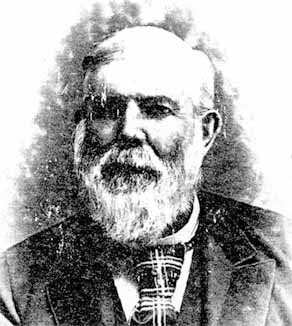
\includegraphics[height=1in]{prologue/pix/shanks.jpg}
  \\
  \protect\label{fig:shanks}\protect\href{https://en.wikipedia.org/wiki/William_Shanks}{William Shanks，1812--1882} % From https://mathshistory.st-andrews.ac.uk/Biographies/Shanks/, PD because of age.
  \protect\end{center}


  一位著名的计算员是 W. Shanks（尚克斯）。
  他的爱好是计算数学常数。
  他于 1873 年发表了将~$\pi$ 计算到小数点后 $707$ 位的结果，但只有前 $527$ 位是正确的。
  （大约在 1820 年，C. Babbage（巴贝奇）设计差分机，正是为了应对由人类计算员完成的对数表计算中的错误。）
  \protect

\begin{center} \protect\small
    \protect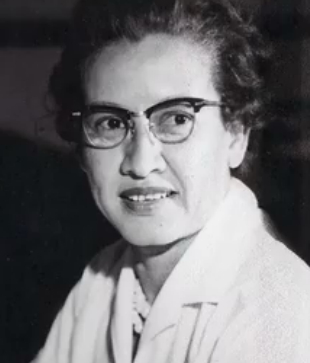
\includegraphics[height=1in]{prologue/pix/katherinejohnson.jpg}
  \\
  \protect\label{fig:johnson}\protect\href{https://bitchmedia.org/article/african-american-women-worked-some-nasas-first-computers}{Katherine Johnson（凯瑟琳·约翰逊），1918--2020，于 2015 年接受总统自由勋章} % NASA/Bill Ingalls, from https://commons.wikimedia.org/wiki/File:Katherine_Johnson_medal.jpeg 
  \protect\end{center}

另一个例子，正如电影《隐藏人物》所述，
多趟美国太空飞行（包括宇航员 John Glenn 的历史性绕地轨道飞行）的轨迹，
都是由人工计算员 Katherine Johnson（凯瑟琳·约翰逊）\protect\index{Johnson, K!picture}和她的同事们通过手算乘法求出的。
她们都是非裔美国女性，她们的成就之所以更加令人敬佩，是因为这是在骇人的歧视之下取得的。}%
正在手工求乘法。
此人遵循一套分步的规程，使用纸笔进行计算，在纸上写满一列列数字。
以此为原型，Turing 为计算员设定了条件。

%<*discussion:DefTuringMachinei>
第一个条件是，它（或者他/她）有一个存储设备（比如计算员的那张纸），可以在上面存放信息，以供后续取用。
% The clerk's paper is two-dimensional but that is
% is not essential, since we could stretch out the work
% into a one-dimensional strip.
%</discussion:DefTuringMachinei>

%<*discussion:DefTuringMachineii>
第二个条件是，这位计算员必须遵循一个确定的程序，一套精确的、不得自由发挥的指令。
程序之所以具有确定性，第一大原因是指令
\citetext{不涉及随机方法}{%
  我们完全可以造出给出纯随机结果的东西；
  例如，有一种装置会记录 Geiger 计数器连续发出的咔咔声，
  如果第二次发出声音间隔比第一次更长，就返回~$1$，
  否则返回~$0$。
  另见
  \protect\url{https://blog.cloudflare.com/randomness-101-lavarand-in-production/}.}，
比如不会通过数放射性衰变产生的咔咔声来决定要执行两种可能操作中的哪一种。

第二大原因是计算员是离散的，它不使用
\citetext{连续方法}{%
  在有计算机之前，工程师有时会使用模拟模型，其中有些规模相当庞大，
  参见 \autocite{wiki:Mississippi}。
  在这类模型中，并不存在什么“第一步、第二步”的概念。}
或
\citetext{模拟设备}{%
  关于计算尺，参见 \autocite{avgeeks}；
  关于列线图，参见 \autocite{wiki:Nomogram}；
  关于海军火控计算机，参见 \autocite{navyreviewer}；
  关于一台更通用的机械计算机，参见 \autocite{vimeo:MechComputer}。
  关于安提基特拉机械装置，参见 \url{https://www.youtube.com/watch?v=qqlJ50zDgeA}。
  关于更现代的设计，请参见
  \url{https://youtu.be/IgF3OX8nT0w?si=hiX4gp9O5QViQCp_} 和
  \url{https://www.youtube.com/watch?v=GVsUOuSjvcg}.}。
因此不存在关于操作精度的疑问，这点不像\citetext{从仪表盘或计算尺读取结果}{%
  假设一个计算的中间结果是 $1.23$。
  如果我们按照分辨率精度只有一位小数的约定从计算尺上读取它，
  那么我们记下~$1.2$。
  将其翻倍得到 $2.4$。
  但将原始数字翻倍 $2\cdot 1.23=2.46$，
  然后四舍五入到一位小数，得到 $2.5$.}那样。
与之相应，计算员也一步一步地工作。
必要时，它可以在完整一步之后暂停，记下自己当前做到哪里
（“正要进位一个 $1$”），过一会儿再接着做。
我们说，在每一时刻，计算员都处于有限多个可能的
\definend{状态}之一，\index{state}
这些状态我们记作 $q_0$、$q_1$、\ldots\sentencespace。
%</discussion:DefTuringMachineii>

%<*discussion:DefTuringMachineiii>
Turing 还增加了第三个条件，这是因为他想研究的是什么东西在原则上是可计算的。
因此，可用存储量
\citetext{不设上限}{%
  这个阐释源自
  \autocite{Rogers}, 第 1--5 页。}。
更准确地说，他不设有限的上限\Dash
如果一次计算眼看就要耗尽存储空间，那存储空间就会
\citetext{自动增长}{%
  也许职员有个助手，或者机器有专人看管。}。
输入或输出的量不设上限，输入和输出之外所需的额外存储（暂存内存）也不设上限。\footnote{%
  确实，撇开云存储不谈，每一台现有的物理计算机的内存都是有限的。
  然而，那个空间极其庞大。
  在本部分，当使用模型设备时，对内存施加限制是一种阻碍，顶多也只是无关紧要。}
同样地，指令的数量也不设上限。
计算在完成前需要执行的步骤数量也不设上限。\footnote{%
  有些作者将像内存量这类资源的可用性描述为“无限”。
  Turing 本人就是这样做的。
  \citetext{读者可能会反对，认为这违背了此定义的目标，
    即对原则上是物理可实现的计算进行建模}{%
     我们都知道有些计算没有自然界限。
     我们小学时学的长除法算法，
     无论是输入或输出的长度，还是可用草稿纸的数量，
     都没有内在的上限。}。% https://cs.stackexchange.com/a/100325/67754
  因此，
  这里的论述换了一种说法：
  这些资源并没有有限的上界。
  不过说真的，怎么表述并不重要。
  两种情况的要点都在于：如果某事物在不设界限时都不可计算，
  那么它在任何物理设备上都不可计算。}
%</discussion:DefTuringMachineiii>

%<*discussion:DefTuringMachineiv>
Turing 还面临最后一个问题：计算员需要有多聪明？
例如，它需要会乘法吗？
我们不需要为乘法做一个特殊功能，因为原则上可以通过重复加法来求乘法。
我们甚至不需要加法，因为我们可以重复加1操作来求加法。
就这样，Turing 将计算员简化到非常基本、易于理解的程度，
直至其操作\citetext{如此基本，以至于我们难以想象它们能被进一步分割}{\autocite{Turing}；\autocite{TuringCorr}}，
同时又保持着强大的能力，足以完成任何原则上可完成之事。
%</discussion:DefTuringMachineiv>

\subsection{定义}
基于这些思考，Turing 设想了一个盒子，盒子里装有机械元件，并配有一条纸带。

\begin{center}
   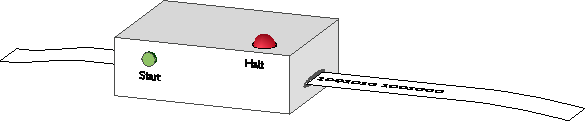
\includegraphics{asy/share/machine00.pdf}
\end{center}

%<*discussion:DefTuringMachinev>
纸带是就是存储器，\index{Turing machine!tape} % \index{memory}
有时也称为“内存”。\index{store, of a machine}
盒子可以从纸带上读取字符，也可以向纸带写入字符，一次一个，
同时还能相对于纸带向任一方向移动读写头\index{read/write head}\index{I/O head|see {read/write head}}\index{Turing machine!read/write head}。
因此，要做乘法的话，
计算员就可以从纸带上读取两个乘数作为输入
（图中显示的是二进制下的
$74$ 和~$72$，中间用空白符隔开），
用纸带做草稿，在计算出结果时停机，并将输出留在纸带上。
%</discussion:DefTuringMachinev>

%<*discussion:DefTuringMachinevi>
盒子就是计算员，也就是 CPU，\index{CPU of Turing machine}\index{Turing machine!CPU}
有时也称为“控制器”。\index{control, of a machine}\index{Turing machine!control}
\texttt{Start}按钮% \index{Start button@\texttt{Start} button}\index{button!start}
用来启动计算。
当计算完成时，
\texttt{Halt}指示灯%\index{Halt light@\texttt{Halt} light}\index{light!Halt@\texttt{Halt}}
会亮起以示停机。
%</discussion:DefTuringMachinevi>
盒子内部的工程实现并不重要\Dash
也许就像我们熟悉的机器那样，它内部有集成电路，
也可能是齿轮和杠杆，又或者是
\index{LEGO}\citetext{乐高积木}{%
  例如参见 \protect\url{https://www.youtube.com/watch?v=RLPVCJjTNgk&t=114s}。}\Dash 重要的是，
它由有限多个部件组成，每个部件
只能处于有限多种状态。
如果它是芯片构成的，那么每个寄存器只有有限多个可能的值；
而如果它是用齿轮或积木搭成的，那么每个部件只能稳定在有限多个可能的位置上。
因此，无论它是如何构造的，
盒子总共只有有限多个状态。

%<*discussion:DefTuringMachinevii>
在执行计算时，机器会逐步从一个状态转移到另一个状态。
例如，
在做乘法时，它可能会根据当前所处的状态以及从纸带上读到的内容，
决定下一步需要进位~$1$。
这时它会转移到一个新状态，
直观上这个新状态就是进行进位操作的地方。

因此，机器的每个步骤涉及四项信息。
我们称
当前状态\index{present state}\index{state!present}\index{Turing machine!present state}为 $q_p$，
下一状态\index{next state}\index{state!next}\index{Turing machine!next state}%
为 $q_n$。
读写头当前指向的符号\index{present tape symbol}\index{Turing machine!present symbol}是 $T_p$。
最后，下一个\index{next tape action}\index{Turing machine!next action}%
纸带动作为~$T_n$。
可能的动作有：在不写入的情况下向左或向右移动读写头，
分别记作 $T_n=\str{L}$ 或~$T_n=\str{R}$，\footnote{%
  我们是
  移动纸带还是移动读写头并不重要，重要的是它们之间的
  相对运动。
  因此 $T_n=\str{L}$ 表示要么纸带、要么读写头移动，使得
  读写头现在指向左侧一格。
  在绘图时，我们保持纸带不动而移动读写头，因为
  这样图形更容易阅读。}
或者在不移动读写头的情况下向纸带写入一个符号，
这时就用该符号表示，因此 $T_n=\str{1}$ 表示机器将向纸带写入一个 \str{1}。
至于字母表，\index{alphabet!tape}\index{tape alphabet@tape alphabet $\Sigma$}\index{input alphabet}
也就是可以出现在纸带上的字符集合，
我们会根据手头的工作选择任何方便的字母表。
但是，
每张纸带上除了有限多个位置外，其余位置都是
空白符\index{blank@blank character \str{B}}\index{tape symbol!blank}，
因此空白符必须是符号之一。
（当空位可能引起混淆时，我们用 $\str{B}$ 表示空白符。）
%</discussion:DefTuringMachinevii>

%<*discussion:DefTuringMachineviii>
这样的四元组 $q_pT_pT_nq_n$ 就是一个\definend{指令}。\index{instruction}\index{Turing machine!instruction}
例如，指令
$\tminstruction{3}{1}{B}{5}$
只有在机器当前处于状态~$q_3$
且正在读取纸带上的符号 \str{1} 时才会执行。
若如此，机器会向纸带写入一个空白符，覆盖掉原来的 \str{1}，
然后转移到状态~$q_5$。
%</discussion:DefTuringMachineviii>

\begin{example} \label{ex:MPred} 
%<*ex:PredecessorTMi>
这台纸带符号集为 $\Sigma=\set{\str{B},\str{1}}$ 的 Turing 机
有六条指令。
\begin{equation*}
 \TM_{\text{pred}}=
  \set{ \tminstruction{0}{B}{L}{1},\,
        \tminstruction{0}{1}{R}{0},\,
        \tminstruction{1}{B}{L}{2},\,
        \tminstruction{1}{1}{B}{1},\,
        \tminstruction{2}{B}{R}{3},\,
        \tminstruction{2}{1}{L}{2} 
      }
\end{equation*}
%</ex:PredecessorTMi>
下方展示了它的一个初始格局。
图中显示了一段纸带，以及机器的状态和读写头的位置。
%<*ex:PredecessorTMii>
\begin{center}
  \tapegraphic{\tmexercises pred000.pdf}
\end{center}
我们采用如下约定：当我们按下 \texttt{Start} 时，机器处于状态 $q_0$。\index{start state@start state $q_0$}\index{state!start}
上图显示机器正在读~$\str{1}$，因此适用指令 $\tminstruction{0}{1}{R}{0}$。
所以第一步是：机器将读写头右移，并保持状态~$q_0$。
%</ex:PredecessorTMii>
下面表格的第一行展示了这一步，
后续行则展示了之后各步的格局。
%<*ex:PredecessorTMiii>
简要来说，读写头先向右滑动，将最后的
\str{1} 置为空白，然后再滑回起点。
\begin{tapesequence}
  \begin{tapesequencetable}
    1 &\tapegraphic{\tmexercises pred001.pdf} \\
    2 &\tapegraphic{\tmexercises pred002.pdf} \\
    3 &\tapegraphic{\tmexercises pred003.pdf} \\
    4 &\tapegraphic{\tmexercises pred004.pdf} \\
    5 &\tapegraphic{\tmexercises pred005.pdf} 
  \end{tapesequencetable}
  \hspace*{2em}
  \begin{tapesequencetable}
    6 &\tapegraphic{\tmexercises pred006.pdf} \\
    7 &\tapegraphic{\tmexercises pred007.pdf} \\
    8 &\tapegraphic{\tmexercises pred008.pdf} \\
    9 &\tapegraphic{\tmexercises pred009.pdf} 
  \end{tapesequencetable}
\end{tapesequence}
至此，由于没有 $q_3\str{1}$ 指令，机器停机。
%</ex:PredecessorTMiii>

%<*ex:PredecessorTMiv>
如果这台机器启动时，初始纸带上除了连续 $n$ 个（$n>0$）\str{1} 外全是空白，且读写头指向其中最左边的那个 \str{1}，那么当机器停机时，纸带上将会有 $n-1$ 个 \str{1}。
如果纸带初始时有 $0$ 个 \str{1}（即全是空白），那么当机器停机时，纸带上也仍是 $0$~个 \str{1}。
也就是说，这台机器计算的是
\definend{前驱函数}\index{predecessor function}\index{function!predecessor}。
\begin{equation*}
  \operatorname{pred}(x)= \begin{cases}
                    x-1  &\case{若 $x>0$}  \\
                    0    &\case{else}
                  \end{cases}
\end{equation*}
%</ex:PredecessorTMiv>
其他示例也延续这一约定：机器启动时读写头指向输入的最左侧符号。
\end{example}

\begin{example} \label{ex:MAdd}
%<*ex:AdditionTMi>
我们可以将这台纸带字母表为 $\Sigma=\set{\str{B},\str{1}}$ 的机器视为在做两个自然数的加法。\index{addition!Turing machine for}\index{Turing machine!for addition}
\begin{align*}
  \TM_{\text{add}} 
  &=
  \{\hspace{\setspacing} \tminstruction{0}{B}{B}{1},\,
        \tminstruction{0}{1}{R}{0},\,
        \tminstruction{1}{B}{1}{1},\,
        \tminstruction{1}{1}{1}{2},\,
        \tminstruction{2}{B}{B}{3},\,        
        \tminstruction{2}{1}{L}{2},\,  \\
        &\qquad\;\tminstruction{3}{B}{R}{3},\,
        \tminstruction{3}{1}{B}{4},\,          
        \tminstruction{4}{B}{R}{5},\,
        \tminstruction{4}{1}{1}{5} 
      \hspace{\setspacing}\}
\end{align*}
输入的两个数字由两串 \str{1} 表示，中间用一个空白符隔开。
%</ex:AdditionTMi>
%<*ex:AdditionTMii>
下图显示了机器准备计算 $2+3$。
\begin{center}
  \tapegraphic{\tmexercises add000.pdf}
\end{center}
%</ex:AdditionTMii>
% We adopt the convention that this is the configuration at step~$0$.
一旦我们按下 \texttt{Start}，机器就向右扫描，
寻找空白分隔符。
它会将那个空白符改写为一个 \str{1}。
接着它掉头向左扫描，直到找到输入的开头。
\citetext{最后，它去掉一个~\str{1}}{%
  指令 $\tminstruction{4}{1}{1}{5}$ 实际上永远不会被触发，
  但这并无妨碍。
  它的存在是为了满足 Turing 机的形式定义，使得
  $\Delta$ 函数在所有的 $q_pT_p$ 上都有定义。
  另请参见该定义的注释。} 
并最终停机，此时读写头指向纸带非空白部分的起始位置。
各步骤如下所示。
%<*ex:AdditionTMiii>
\begin{tapesequence}
  \begin{tapesequencetable}
    1 &\tapegraphic{\tmexercises add001.pdf} \\
    2 &\tapegraphic{\tmexercises add002.pdf} \\
    3 &\tapegraphic{\tmexercises add003.pdf} \\
    4 &\tapegraphic{\tmexercises add004.pdf} \\
    5 &\tapegraphic{\tmexercises add005.pdf} \\
    6 &\tapegraphic{\tmexercises add006.pdf} 
  \end{tapesequencetable}
  \hspace*{2em}
  \begin{tapesequencetable}
     7 &\tapegraphic{\tmexercises add007.pdf} \\
     8 &\tapegraphic{\tmexercises add008.pdf} \\
     9 &\tapegraphic{\tmexercises add009.pdf} \\
    10 &\tapegraphic{\tmexercises add010.pdf} \\
    11 &\tapegraphic{\tmexercises add011.pdf} \\
    12 &\tapegraphic{\tmexercises add012.pdf} 
  \end{tapesequencetable}
\end{tapesequence}
%</ex:AdditionTMiii>
% We can think of this machine as computing the sum of two inputs,  
% $f(x,y)=x+y$.
\end{example}

%<*ex:PredecessorTMv>
除了用列表形式给出机器的指令外，
我们还可以使用表格或图形。
以下是 $\TM_{\text{pred}}$ 的
\definend{转移表}\index{transition table}\index{table, transition}\index{transition function@transition function $\Delta$!table of} 
及其
\definend{转移图}。\index{transition graph}\index{graph!transition}\index{transition function@transition function $\Delta$!graph of}
%</ex:PredecessorTMv>


\begin{center}
  \begin{transitionfunction}[\Delta_{\text{pred}}]
           &$\blank$      &\str{1}        \\ \cline{2-3}
     $q_0$ &$\str{L}q_1$  &$\str{R}q_0$     \\ 
     $q_1$ &$\str{L}q_2$  &$\str{B}q_1$     \\ 
     $q_2$ &$\str{R}q_3$  &$\str{L}q_2$     \\  
     $q_3$ &--            &--     \\
  \end{transitionfunction}
  \hspace{2em}
  \vcenteredhbox{\includegraphics{prologue/asy/circlediagram/circlediagram00.pdf}}
\end{center}


而这是 $\TM_{\text{add}}$ 所对应的表格与图。


\begin{center}
  \begin{transitionfunction}[\Delta_{\text{add}}]
           &$\blank$      &\str{1}        \\ \cline{2-3}
     $q_0$ &$\str{B}q_1$  &$\str{R}q_0$     \\ 
     $q_1$ &$\str{1}q_1$  &$\str{1}q_2$     \\ 
     $q_2$ &$\str{B}q_3$  &$\str{L}q_2$     \\  
     $q_3$ &$\str{R}q_3$  &$\str{B}q_4$     \\  
     $q_4$ &$\str{R}q_5$  &$\str{1}q_5$     \\  
     $q_5$ &--            &--     \\
  \end{transitionfunction}
  \hspace{2em}
  \vcenteredhbox{\includegraphics{prologue/asy/circlediagram/circlediagram01.pdf}}
\end{center}


% The graph is how we will most often present machines that are small 
% but if there are lots of states then it can be visually confusing.

接下来是一个关键观察。
有些 Turing 机，至少对某些起始格局而言，是永不停机的。


\begin{example} \label{ex:TMNeverHalts}
%<*ex:SomeTMsDontHalt>
Turing 机
$
  \TM_{\text{inf loop}}=\set{
        \tminstruction{0}{B}{B}{0},\,
        \tminstruction{0}{1}{1}{0}
      }
$
不论输入是什么都永不停机。
\begin{center}
  \vcenteredhbox{\includegraphics{\asydir circlediagram/infloop.pdf}}
\end{center}
%</ex:SomeTMsDontHalt>
练习中会要求你给出在一些输入上停机、在另一些输入上不停机的 Turing 机例子。
\end{example}

是时候下定义了。
我们将\definend{符号}\index{symbol}\index{tape symbol}定义为设备为了存储和检索而能够写入和读取的事物。\footnote{%
  设备如何做到这一点取决于其具体的构造方式。
  它可以读写纸带上的标记，
  调整塑料磁带上的磁性颗粒排列，
  翻转固态硬盘上的比特位，
  或者将乐高积木推到凹槽的左边或右边。
  离散性要求机器能够清晰地区分不同的符号，而读取接近边界处的仪器刻度盘时则可能会遇到麻烦。}

%<*df:TM>

\begin{definition} \label{def:TuringMachine}
一台\definend{Turing 机（Turing machine）}~$\TM$\index{Turing machine!definition} 
是一个有限的四元组
\definend{指令（instruction）}\index{instruction}\index{Turing machine!instruction} 
集合，指令形如 $q_pT_pT_nq_n$。\footnotemark[2]
在一条指令中，
\definend{当前状态（present state）}~$q_p$\index{present state}\index{Turing machine!present state} 和
\definend{下一状态（next state）}~$q_n$\index{next state}\index{Turing machine!next state} 属于一个
\definend{状态集（set of states）}~$Q$。\index{states!set of Q@set of $Q$} 
\definend{输入符号（input symbol）}\index{symbol!input}\index{Turing machine!input symbol}
或
\definend{当前符号（current symbol）}\index{current symbol}\index{symbol!current}\index{Turing machine!current symbol} 
$T_p$ 属于
\definend{纸带字母表（tape alphabet）}\index{tape alphabet@tape alphabet $\Sigma$}\index{alphabet!tape}\index{alphabet!Turing machine}\index{Turing machine!tape alphabet} 
集合~$\Sigma$，
该集合至少包含两个符号，其中包括一个称为
\definend{空白符（blank）}的符号，\index{blank@blank character \str{B}}
并且不包含 $\str{L}$ 或~$\str{R}$。
\definend{动作符号（action symbol）}~$T_n$\index{symbol!action}\index{Turing machine!action symbol}\index{symbol!action}\index{Turing machine!action symbol} 
属于
\definend{动作集（action set）}~$\Sigma\cup\set{\str{L},\str{R}}$。\index{action set}\index{Turing machine!action set} 

集合~$\TM$ 必须是
\index{determinism}\index{Turing machine!deterministic}\definend{确定性的（deterministic）}：不同的
四元组不能以
相同的 $q_pT_p$ 开头。
因此，在指令集 $q_pT_pT_nq_n\in\TM\!$ 上，
从当前对 $q_pT_p$ 到下一对~$T_nq_n$ 的关联
定义了一个函数，即
\citetext{\definend{转移函数（transition function）}}{%
  定义将 $\Delta$ 描述为一个函数
  $\map{\Delta}{Q\times \Sigma}{(\Sigma\cup\set{\str{L},\str{R}})\times Q}$。
  这其实是一种权宜之计。
  在 $\TM_{\text{pred}}$ 中，状态 $q_3$ 仅用于使机器停机，因此没有定义下一状态。
  在 $\TM_{\text{add}}$ 中，状态~$q_5$ 扮演了同样的角色。
  所以，严格来说，转移函数是一个偏函数（partial function），即其定义域中的某些成员没有对应的
  值；参见第~\pageref{def:PartialFunction}~页。
  （或者，我们可以把状态集写成
  $Q\cup\hat{Q}$，其中 $\hat{Q}$ 里的状态仅用于
  停机，而转移函数的定义为
  $\map{\Delta}{Q\times \Sigma}{(\Sigma\cup\set{\str{L},\str{R}})\times (Q\cup\hat{Q})}$。）
  我们在主要叙述中略去了这一点，
  因为通常不会引起混淆，深入讨论反而可能分散注意力。}\index{transition function@transition function $\Delta$!Turing machine}\index{function!transition}\index{Turing machine!transition function}
或称
\definend{下一状态函数（next-state function）}\index{next-state function|see{transition function}}\index{function!next-state|see{transition function}}\index{Turing machine!next-state function}
$\map{\Delta}{Q\times \Sigma}{(\Sigma\cup\set{\str{L},\str{R}})\times Q}$。 
\end{definition}

\footnotetext[2]{%
  我们用 $\TM$ 来表示 Turing 机，是因为尽管这些机器
  是硬件，
  但它们最像我们日常经验中的程序。}
%</df:TM>

% %<*df:TMnote>
% We denote Turing machines with a $\TM$ because, although they are hardware, 
% the things from everyday experience that they are most like are programs.
% %</df:TMnote>

当然，这些机器的关键在于它们能做什么。
为了完成形式化，我们现在给出
\citetext{对机器动作的完整描述}{%
  一个很合理的问题是：为什么我们的标准模型——Turing 机——
  如此基础，以至于为它编程
  可能很繁琐？
  为什么不选一个真实世界里的机器呢？
  原因是，我们可以用仅仅几段话就完全描述 Turing 机模型的
  动作
  动作。
  而一台真实的机器本身就需要一整本书来描述。
  此外，Turing 机具有历史
  重要性，而且第五章的工作也需要它们。}。

\label{text:DescriptionOfTMAction}
回顾\zcref{ex:MPred}和\zcref{ex:MAdd}的执行过程可以清楚地看到，Turing 机是通过控制机器排布之间的转移来运作的。
%<*def:TMConfigurationi>
Turing 机的一个
\definend{格局（configuration）}\index{configuration!Turing machine}\index{Turing machine!configuration}  
是一个四元组$\sequence{q,s,\tau_L,\tau_R}$，其中
\citetext{$q$ 是一个状态}{% 
  我们对“状态”究竟是什么并未给出严格定义。
  正式的字典定义称其为机器的一种“模式”
  \url{https://www.merriam-webster.com/dictionary/state}，
  但这只是用一个词替换了另一个词。
  为了直观理解，我们可以想象一台由多个齿轮构成的机器。
  那么，状态就是所有可能的齿轮组合，
  例如齿轮四的第六个齿嵌入齿轮五的第七个槽中，使两者啮合。
  在一台笔记本电脑上，状态集由所有可能的寄存器及其内容的组合构成，
  例如寄存器八包含 \str{101010}。}，
$s$ 是来自纸带字母表~$\Sigma$ 的一个字符，
而 $\tau_L$ 和~$\tau_R$ 是来自~$\kleenestar{\Sigma}\!$ 的串，
也可能是空串~$\emptystring$。\index{empty string@empty string, $\emptystring$}\index{string!empty}
它们分别表示当前状态、读写头下的字符、以及读写头左侧和右侧的纸带内容。
%</def:TMConfigurationi>
例如，在\zcref{ex:MAdd}的跟踪表中，
“步骤~$2$” 这一行显示，经过两次转移后，
状态是 $q=q_0$，
读写头下的字符是空白符 $s=\str{B}$，
读写头左侧是 $\tau_L=\str{11}$，
读写头右侧是 $\tau_R=\str{111}$。
因此，该行的图示描绘了格局
$\sequence{q_0,\str{B},\str{11},\str{111}}$。
换句话说，格局是
\citetext{一个快照，即计算中的一个瞬间}{%
  因此，格局连同 Turing 机就是你继续该计算所需的所有信息\Dash 它封装了该计算的未来历史。}。

\label{DefnConfiguration}
%<*def:TMConfigurationii>
我们用 $\configuration(t)$ 表示机器在第 $t$ 次转移后的格局，并称之为
\definend{步骤}~$t$ 时的格局。\index{step of a computation}\index{computation!step}
我们将此定义扩展到步骤~$0$，规定
\definend{初始格局（initial configuration）}\index{initial configuration!Turing machine}\index{configuration!initial!Turing machine} 
$\configuration(0)$
是我们在按下 \texttt{Start} 键之前机器的格局。
%</def:TMConfigurationii>

接下来定义其动作：假设在步骤~$t$，
机器 $\TM$ 处于格局
$\configuration(t)=\sequence{q,s,\tau_L,\tau_R}$。
为了进行下一次转移，寻找一条
形如 $q_pT_pT_nq_n\in\TM$ 的指令，其中
$q_p=q$ 且~$T_p=s$。
确定性条件确保了集合~$\TM$ 中至多有一条这样的指令。
如果没有这样的指令，那么在
步骤~$t+1$，机器 $\TM$ 就会\definend{停机（halts）}。
此时的格局就是它的
\definend{停机格局（halting configuration）}。\index{halting configuration!Turing machine}\index{configuration!halting!Turing machine}\index{Turing machine!halting configuration}

否则，有三种可能性。
(1)~如果 $T_n$ 是纸带字母表集合~$\Sigma$ 中的一个符号，那么
机器将该符号写入纸带，因此
下一个格局是
$\configuration(t+1)=\sequence{q_n,T_n,\tau_L,\tau_R}$，其定义如下。
(2)~如果 $T_n=\str{L}$，那么机器将读写头向左移动。
更准确地说，下一个格局是  
$\configuration(t+1)=\sequence{q_n,\hat{s},\hat{\tau}_L,\hat{\tau}_R}$。
% where $\hat{s}$ is the rightmost character of the string~$\tau_L$,
% where $\hat{\tau}_R$ is the result of pushing the character~$s$
% onto the string~$\tau_R$,
% and where $\hat{\tau}_L$ is $\tau_L$ with its rightmost character omitted.
% (More precisely,
其新的右侧纸带 
$\hat{\tau}_R$ 是由单字符的串
$\sequence{s}$ 与先前格局的 $\tau_R$ 拼接而成。
至于 $\configuration(t+1)$ 的新左侧纸带和新的当前
字符，有两种情况：当 
$\tau_L=\emptystring$ 时，$\hat{s}$ 是空白符
且 $\hat{\tau}_L=\emptystring$，
而当 $\tau_L\neq\emptystring$ 时，新的当前字符 $\hat{s}$ 是  
$\tau_L$ 的最右字符，即 $\hat{s}=\tau_L[-1]$， 
而新的左侧纸带 $\hat{\tau}_L$ 
则是 $\tau_L$ 去掉最右字符后余下的部分，即
$\hat{\tau}_L=\tau_L[\,:-1]$。
(3)~如果 $T_n=\str{R}$，那么机器将读写头向右移动。
这与~(2) 非常相似，故省略细节。

%<*def:TMConfigurationiii>
如果两个格局通过一步转移相关联，
那么我们记作
$\mathcal{C}(i) \yields \mathcal{C}(i+1)$。\footnote{% 
  将 `$\,\yields$' 读作“转移为”。
  % We could, where $\mathcal{I}$ is the applicable instruction,
  % write~$\yields_{\mathcal{I}}$,  
  % but we will never need to do that.
  }\index{yields@yields $\yields$!for Turing machines}
一个\definend{计算（computation）}\index{computation!Turing machine}\index{Turing machine!computation} 
是一个序列
$
  \mathcal{C}(0) \yields \mathcal{C}(1) \yields \mathcal{C}(2)
   \yields \cdots\, 
$。
我们用 $\kleenestar{\yields}$ 来缩写一连串的 $\yields$。\footnote{% 
  读作“最终转移为”。} %\index{yields eventually!$\kleenestar{\yields}$for Turing machines} 
如果计算停机，那么序列有一个最终的
格局~$\mathcal{C}(h)$ 
因此我们可以将一次停机计算写作
$\mathcal{C}(0)\mathrel{\kleenestar{\yields}}\mathcal{C}(h)$。
%</def:TMConfigurationiii>

\begin{example} \label{ex:TraceComputation}
  在\zcref{ex:MPred}追踪机器步骤的表格中，图形展示了相继的格局
  （注意初始图形在表格之前）。
下面将同一序列展示为一个计算。
\begin{multline*}
\sequence{q_0,\str{1},\emptystring,\str{11}}
\yields
\sequence{q_0,\str{1},\str{1},\str{1}}
\yields
\sequence{q_0,\str{1},\str{11},\emptystring}
\yields
\sequence{q_0,\str{B},\str{111},\emptystring}
\yields
\sequence{q_1,\str{1},\str{11},\emptystring}  \\
\yields
\sequence{q_1,\str{B},\str{11},\emptystring}
\yields
\sequence{q_2,\str{1},\str{1},\emptystring}
\yields
\sequence{q_2,\str{1},\emptystring,\str{1}}
\yields
\sequence{q_2,\str{B},\emptystring,\str{11}}
\yields
\sequence{q_3,\str{1},\emptystring,\str{1}}
\end{multline*}
\end{example}

关于这些细节，还有最后一点。
我们已经将计算定义为一个物理系统通过一系列离散步骤演化的过程。
\citetext{注意，这种演化是局部的，因为所有动作都发生在读写头所在的一个单元格内}{%
    改编自 \autocite{WigdersonMC}。}。

% Finally, as in that example,
% observe that our description of the action of a Turing machine
% emphasizes that it is a
% \citetext{\index{state machine}}{%
%   A state machine is a device that stores the status of something at a
%   given time.
%   On input it can change the status (it can also cause an action or
%   output to take place).
%   Mathematically, it is a finite set $Q=\set{q_0,\ldots q_n}$ along with
%   a function $\map{\Delta}{Q\times\Sigma}{Q}$.}\index{machine!state}\definend{state machine}\Dash
% a computation is a sequence of discrete transitions.

\subsection{可计算函数}\index{computable function|(}
在本章开头我们曾表示，相对于计算如何进行，我们对机器计算出的东西更感兴趣。\footnote{%
  这与编程课程形成对比，编程课需要投入大量精力学习如何将复杂任务分解为更简单的子任务，如何在子任务间建立可靠的接口等。}
本节最后，我们将定义可以被机械计算的函数集合。

%<*df:FcnComputedByTMi>
函数是输入与输出之间的一种关联。
对于 Turing 机，自然的关联是：将机器启动时纸带上的串与它停机时纸带上的串联系起来。
这样我们就得到了一个从串到串的函数，如
$\TMfcn(\str{111})=\str{11111}$，就像这里一样。
\begin{equation*}
 \vcenteredhbox{\includegraphics{\asydir tape/tapefcn0.pdf}} 
  \quad\mapsto\quad
  \vcenteredhbox{\includegraphics{\asydir tape/tapefcn1.pdf}}
\end{equation*}
%</df:FcnComputedByTMi>
\noindent
但该定义必须注意几个问题。
首先，Turing 机可能在某些输入串上不停机。
其次，
仅仅指定输入串还不够，因为读写头的初始位置会影响计算。

%<*df:FcnComputedByTMii>


\begin{definition} \label{def:FcnComputedByTM}
  设 $\TM$ 是一台纸带字母表为 $\Sigma$ 的 Turing 机。
  对于输入 $\sigma\in\kleenestar{\Sigma}\!$，
  将该串放置在其他位置均为空白的纸带上，并将 $\TM$ 的读写头指向 $\sigma$ 最左边的符号，这一过程称为对该输入的
  \definend{装载}\index{loading input on tape}\index{input!loading}。
  如果我们以装载好 $\sigma$ 的状态启动 $\TM$ 且它最终停机，
  那么我们将关联的输出串记作
  \definend{$\TMfcn_{\TM}(\sigma)$}。
  如果机器永不停机，则 $\sigma$ 没有关联的输出。
\definend{机器计算的函数}~$\TM$\index{function!computed by a Turing machine}\index{Turing machine!function computed}
  是所有关联 $\sigma \mapsto \TMfcn_{\TM}(\sigma)$ 的集合。
\end{definition}


%</df:FcnComputedByTMii>

%<*df:FcnConverge>


\begin{definition}
对于 $\sigma\in\kleenestar{\Sigma}\!$，
如果 Turing 机计算的值在 $\sigma$ 上没有定义，
那么我们称机器计算的函数在该输入上
\definend{发散}，\index{diverge}\index{function!diverge}
记作\definend{$\TMfcn_{\TM}(\sigma)\mathord{\uparrow}$}
（或 $\TMfcn_{\TM}(\sigma)=\bot$\,）。
否则我们称它在该输入上
\definend{收敛}，\index{converge}\index{function!converge}
\definend{$\TMfcn_{\TM}(\sigma)\mathord{\downarrow}$}。
\end{definition}


%</df:FcnConverge>

%<*discussion:FcnVsMachine>
注意区分机器 $\TM$ 和该机器计算的函数 $\TMfcn_{\TM}$。
例如，
机器 $\TM_{\text{pred}}$ 是一个四元组的集合，
但前驱函数是一个输入-输出对的集合，
我们可以将其记作 $x\mapsto \operatorname{pred}(x)$。
另一个区别的例子是：机器停机或不停机，而函数收敛或发散。
%</discussion:FcnVsMachine>

还有几点：


\begin{parenum}
\item
当讨论中只有一台机器时，我们写作 $\TMfcn$ 来代替 $\TMfcn_{\TM}$。
\item
在本书中，我们倾向于构造这样的机器，使其在结束时读写头也位于输出串的第一个字符下方，
这并非严格必要，但使得组合机器更容易。
\item
在大多数数学领域中，函数都有一个定义域，即其有定义的那些输入构成的集合。
在本领域，一个关键特性是机器可以接收一个输入串，却永不返回输出，因为它不停机。
因此在这里，我们常写作
$\map{\phi}{\kleenestar{\Sigma}}{\kleenestar{\Sigma}}$
并将其描述为一个
\definend{偏函数}，\index{partial function}\index{function!partial}
其中某个
$W\subseteq\kleenestar{\Sigma}$ 是所有使得 $\phi(\sigma)\converges$ 的输入串 $\sigma$ 的集合。
如果 $W=\kleenestar{\Sigma}$，则称 $\phi$ 是一个
\definend{全函数}。\index{total function}\index{function!total}
（每个 $\phi$ 都是偏的，但说“偏”通常意味着该函数不是全的。）\footnote{%
  更多内容参见附录~\protect\ref{sec:Functions}。}
\end{parenum}

% There is one last point to raise about the definition.
%<*discussion:FcnConverge>
我们常常会考虑那些并非从串到串的映射的函数，并将它们描述为由机器计算的函数。
为此，我们必须对输入和输出赋予一种解释。
一个例子是\zcref{ex:MPred}中的前驱机，在那里我们把串解释为一元表示的自然数。
% The same holds for computations with non-numbers.
% \footnote{%
%   In the example of the addition machine, \protect\zcref{ex:MAdd},
%   we took the separator blank to be significant.
%   Allowing significant blanks
%   opens the possibility of ambiguity:~which of the 
%   blanks at the beginning and end of the input and output strings
%   count and which do not?
%   There are a number of ways that we could handle this.
%   We could add a character to the alphabet to use exclusively as a begin/end
%   marker.
%   Or we could enforce that strings
%   come in the form $\sigma=1^n\str{B}\tau$
%   where the length of $\tau$ is~$n$
%   (so that any time we change $\tau$'s length we
%   must adjust the~$n$).
%   Perhaps the most mathematically pleasant is to  
%   code everything that we want to say with integers, in unary.
%   Thus, we could code the triple of numbers $\sequence{7, 8, 9}$
%   as the
%   single number $2^7 3^8 5^9\!$, using the uniqueness of
%   prime factorization.
%   In this book
%   we leave off this disambiguation because
%   it hides the underlying ideas (see 
%   also \zcref{rem:EarlyResearchersAirtightArgs}).
% }
% The machine just runs, it is up to us to give the actions a sense.
当然，物理计算机上也发生着同样的事情，机器摆弄着比特串，然后我们将它们解释为文档中的字符、四重奏中的音符，或者任何我们喜欢的东西。\footnote{%
  我们或许会担心，我们的解释可能会变得如此复杂，以至于像占星术一样，实际工作都发生在解释过程中。
  但我们将坚持讨论像自然数的一元表示法这样不存在这一问题的情况。}

当我们描述由机器计算的函数时，我们通常会省略解释串的部分。
我们会说，“这表明 $\TMfcn(3)=5$”
\citetext{而不是说，“这表明 $\TMfcn$ 将一个代表~$3$ 的串映射为一个代表~$5$ 的串。”}{%
  也就是说，我们这样做，理由和我们说“这是我十岁的时候”
  而不是说“这是我十岁时的一张照片”一样。}
表示的细节通常在这一章里无关紧要
（在第五章，我们有时会关心它们消耗的时间或空间）。
%</discussion:FcnConverge>

\begin{remark} \label{rem:EarlyResearchersAirtightArgs}
早期的研究者在实际机器尚未普及之前工作，他们需要严密的证明，例如，存在一种机械计算，能够计算这样的函数：输入一个数，返回该数素数分解中 $5$ 的幂次。
因此他们处理了这些细节，积累了大量可能相当底层的工作成果。

作为一个底层细节的例子，在加法机\zcref{ex:MAdd}中，我们把分隔用的空白符视为有意义的。
允许有意义的空白符带来了歧义性问题：纸带上哪些空白符算作输入和输出，哪些不算？
我们可以通过给字母表增加一个专门用作开始/结束标记的字符来处理。
或者，我们可以强制要求串以 $\sigma=\alpha\str{B}\tau$ 的形式出现，其中 $\tau$ 由 $\lh{\alpha}$ 个 \str{1} 组成。
又或者，我们可以用整数编码一切，例如将三元组 $\sequence{7, 8, 9}$ 编码为 $2^7 3^8 5^9\!$。

在本书中，我们通常不坚持这种细节程度。
我们的日常经验使我们相信，机器可以用它们的字母表合理地表示任何可计算的东西。
此外，在细节上花费大量时间有掩盖核心思想的风险，而我们希望进入更有趣的内容。
下一节会对此有更多说明。
\end{remark}

%<*df:ComputableFcn>


\begin{definition} \label{def:ComputableFcn}
一个\definend{可计算函数},\index{computable function!definition}\index{function!computable} 
或 \index{recursive function}\index{function!recursive}\definend{递归函数},\footnotemark[1]
是由某个 Turing 机计算的函数（它可以是全函数或偏函数）。
一个\definend{可计算集},\index{computable set}\index{set!computable} 
或\definend{递归集},\index{recursive set}\index{set!recursive} 
是其特征函数可计算的集合。
一个关系是可计算的\index{computable relation}\index{relation, computable}，当且仅当它作为集合是可计算的。\footnotemark[2]
\end{definition}

\footnotetext[1]{%
  “递归”这个术语曾经是通用的，但现在已有些过时。}
\footnotetext[2]{%
  例如，“小于”关系是可计算的，因为存在一个可计算函数，输入两个整数 $a$ 和~$b$，如果 $a<b$ 则返回~\str{1}，否则返回 \str{0}。}
%</df:ComputableFcn>

% There is a terminology focused on Boolean functions that we will
% emphasize in Chapter Five.

%<*df:TMDecidesLanguage>

\begin{definition} \label{df:TMDecidesLanguage}
若一台 Turing 机计算某集合的特征函数，则称它
\definend{判定}此集合。\index{Turing machine!decide a set}\index{set!decided by a Turing machine}
也就是说，对于所有属于该集合的输入，机器都停机并接受
（或许通过纸带最终只留下 \protect{\str{1}} 来表示），
而对于所有不属于该集合的输入，机器都停机并拒绝
（或许纸带最终全是空白）。\index{Turing machine!decide a language}\index{language!decided by a Turing machine}\index{decides!a language}
若一台 Turing 机对于所有属于某集合的输入都停机并接受，而对于非成员输入，
它从不以接受状态停机（但它可能不停机），则称它\definend{识别}
此集合。\index{Turing machine!recognize a set}\index{set!recognized by a Turing machine}\index{recognized set}
\end{definition}

%</df:TMDecidesLanguage>

\medskip
最后我们总结一下。
我们已经为直观上的机械可计算性给出了一个精确的定义，
从而精确刻画了哪些函数能够被机械计算。
下一小节将讨论为什么这一刻画被广泛接受。
\index{computable function|)}

% -------------------------------------------
\begin{exercises}[除非练习题另有说明，
假设 $\Sigma=\set{\str{B},\str{1}}$。
同时假设任何机器都必须将其读写头起始位置放在最左输入字符下方，
并使其在完成时读写头位于最左输出字符下方。]

\begin{exercise}
Turing 机在哪些方面像一个程序？
在哪些方面不像？
在哪些方面像我们桌上的那种电脑？
在哪些方面不像？
\begin{answer}
它像程序的地方在于它是单一用途的，也就是说，
就像我们可以有一个仅将输入翻倍而不做其他事情的程序一样，
我们也可以有这样一个 Turing 机。
它不像程序的地方在于它是硬件。

它像我们今天桌上电脑的地方在于它机械地将输入转换为输出。
Turing 机不像这种电脑的地方在于它是为单一任务而特制的。
\end{answer}
\end{exercise}

\begin{exercise}
\begin{credit}
  SE 用户 Shuzheng, https://cs.stackexchange.com/q/45589/50343
\end{credit}
为什么 Turing 机的定义（\zcref{def:TuringMachine}）不包括对纸带内容的定义？
% It includes the tape alphabet~$\Sigma$, but not the sequence of alphabet 
% characters that make up the tape.
\begin{answer}
这个定义描述的是机器本身。
关于机器动作的进一步描述，包括格局和转移的定义，
紧随\zcref{def:TuringMachine}之后。
在某种程度上，这是对\zcref{def:TuringMachine}的扩展。

换言之，正如 A~Bauer 在 Stack Exchange 上对此问题的评论中所说，
为什么道路不是汽车的一部分？
\end{answer}
\end{exercise}

\begin{exercise}
\begin{credit}
  问题由 SE 用户 Arsalan MGR 提出，\url{https://cs.stackexchange.com/q/135343/50343}
\end{credit}
你的学习伙伴问道：
“开篇段落提到\textit{Entscheidungsproblem}，即机械地判定一个数学陈述是真还是假。
我经常写带有布尔判断子句的程序，比如‘\texttt{if (x>3)}’。
这有什么问题呢？”
请帮他们解惑。\index{Entscheidungsproblem@\textit{Entscheidungsproblem}}\index{decision problem}
\begin{answer}
这并不是判断某个特定数学陈述是否为真的问题。
显然，如果 $x=2$，那么我们就可以判断 $x>3$ 是否成立。
类似地，我们可以判定 $\forall x\in\N\;[x^2>3]$ 的真假。
而\textit{Entscheidungsproblem} 要求的是一个算法，
它能输入任意数学陈述，并输出 `\true' 或 `\false'。
\end{answer}
\end{exercise}

\recommended

\begin{exercise}
像\zcref{ex:TraceComputation}中那样，追迹下列每次计算。
\begin{exparts*}
\item
追迹例~\ref{ex:MPred}中的机器 $\TM_{\text{pred}}$ 在含有两个 \str{1} 的纸带上启动时的计算。
\item
追迹例~\ref{ex:MAdd}中的机器 $\TM_{\text{add}}$ 在两个加数分别为 $2$ 和~$2$ 时的计算。
\item 如\zcpageref{DefnConfiguration}页所述，以格局序列的形式给出这两个计算。
\end{exparts*}
\begin{answer}
\begin{exparts}
\item 以下是计算 $2$ 的前驱过程中产生的纸带序列。
\begin{tapesequence}
  \begin{tapesequencetable}
    0 &\tapegraphic{\tmexercises pred_two000.pdf} \\
    1 &\tapegraphic{\tmexercises pred_two001.pdf} \\
    2 &\tapegraphic{\tmexercises pred_two002.pdf} \\
  \end{tapesequencetable}
  \hspace*{2em}
  \begin{tapesequencetable}
    3 &\tapegraphic{\tmexercises pred_two003.pdf} \\
    4 &\tapegraphic{\tmexercises pred_two004.pdf} \\
    5 &\tapegraphic{\tmexercises pred_two005.pdf} \\
  \end{tapesequencetable}
  \hspace*{2em}
  \begin{tapesequencetable}
    6 &\tapegraphic{\tmexercises pred_two006.pdf} \\
    7 &\tapegraphic{\tmexercises pred_two007.pdf} \\
  \end{tapesequencetable}
\end{tapesequence}
\item 这是 $2$ 与~$2$ 求和的纸带图序列。
\begin{tapesequence}
  \begin{tapesequencetable}
    0 &\tapegraphic{\tmexercises addtwotwo000.pdf} \\
    1 &\tapegraphic{\tmexercises addtwotwo001.pdf} \\
    2 &\tapegraphic{\tmexercises addtwotwo002.pdf} \\
    3 &\tapegraphic{\tmexercises addtwotwo003.pdf} \\
    4 &\tapegraphic{\tmexercises addtwotwo004.pdf} \\
  \end{tapesequencetable}
  \hspace*{2em}
  \begin{tapesequencetable}
    5 &\tapegraphic{\tmexercises addtwotwo005.pdf} \\
    6 &\tapegraphic{\tmexercises addtwotwo006.pdf} \\
    7 &\tapegraphic{\tmexercises addtwotwo007.pdf} \\
    8 &\tapegraphic{\tmexercises addtwotwo008.pdf} \\
    9 &\tapegraphic{\tmexercises addtwotwo009.pdf} \\
  \end{tapesequencetable}
  \hspace*{2em}
  \begin{tapesequencetable}
   10 &\tapegraphic{\tmexercises addtwotwo010.pdf} \\
   11 &\tapegraphic{\tmexercises addtwotwo011.pdf} \\
   12 &\tapegraphic{\tmexercises addtwotwo012.pdf} \\
  \end{tapesequencetable}
\end{tapesequence}
\item 以下是前驱计算的格局序列。
\begin{align*}
  &\sequence{q_0,\str{1},\emptystring,\str{1}}
   \yields\sequence{q_0,\str{1},\str{1},\emptystring}
   \yields\sequence{q_0,\str{B},\str{11},\emptystring}
   \yields\sequence{q_1,\str{1},\str{1},\emptystring}
   \yields\sequence{q_1,\str{B},\str{1},\emptystring}
   \yields\sequence{q_2,\str{1},\emptystring,\emptystring}  \\
   &\qquad\yields\sequence{q_2,\str{B},\emptystring,\str{1}} 
   \yields\sequence{q_3,\str{1},\emptystring,\emptystring}
\end{align*}
由于状态 $q_3$ 没有对应的指令，因此 $\sequence{q_3,\str{1},\emptystring,\emptystring}$ 是一个停机格局。

$2$ 与 $2$ 相加的计算序列稍长一些。
\begin{align*}
   &\sequence{q_0,\str{1},\emptystring,\str{1B11}}
   \yields\sequence{q_0,\str{1},\str{1},\str{B11}}
   \yields\sequence{q_0,\str{B},\str{11},\str{11}}
   \yields\sequence{q_1,\str{B},\str{11},\str{11}}
   \yields\sequence{q_1,\str{1},\str{11},\str{11}}  \\  
   &\qquad\yields\sequence{q_2,\str{1},\str{11},\str{11}}
   \yields\sequence{q_2,\str{1},\str{1},\str{111}}  
   \yields\sequence{q_2,\str{1},\emptystring,\str{1111}}
   \yields\sequence{q_2,\str{B},\emptystring,\str{11111}}  \\  
   &\qquad\yields\sequence{q_3,\str{B},\emptystring,\str{11111}}
   \yields\sequence{q_3,\str{1},\emptystring,\str{1111}}
   \yields\sequence{q_4,\str{B},\emptystring,\str{1111}}
   \yields\sequence{q_5,\str{1},\emptystring,\str{111}}
\end{align*}
\end{exparts}
\end{answer}
\end{exercise}

\recommended

\begin{exercise}
对于下列关于 Turing 机的错误陈述，简要指出其谬误所在。
\begin{exparts*}
\item Turing 机不能处理负数，因此它不是一个完备的计算模型。
\item \zcref{ex:TMNeverHalts}中的问题在于，指令中没有额外的状态让机器去停机。
\item 一台机器要达到状态 $q_{50}$，它必须至少运行五十一步。
\end{exparts*}
\begin{answer}
\begin{exparts}
\item 要证明对负数（或其他任何数学对象）的某些操作是可计算的，需要先为它们指定一种基于有限字母表上字符串的表示方法，然后展示如何使用 Turing 机对这些字符串进行机械计算。
例如，要证明两个整数的乘法是机械的，我们可以使用字母表 $\Sigma=\set{\str{B},\str{0},\ldots \str{9},\str{+},\str{-}}$ 并将每个整数表示为一对 $\sequence{\text{sign},\text{自然数}}$。构造一台 Turing 机来处理四种可能的符号组合情况，虽然繁琐但完全可行。
\item 如果这里说的“问题”是指机器不停机，那么这并不是问题的根源。相反，这台机器只是一个简单的无限循环。
\item 我们可以给机器设定非顺序编号的状态。唯一的限制是我们遵循初始状态为 $q_0$ 的约定。例如，机器 $\TM=\set{\tminstruction{0}{B}{B}{50},\,\tminstruction{0}{1}{1}{50},\,\tminstruction{50}{1}{1}{1},\,\tminstruction{50}{1}{1}{1}}$ 符合定义，并且在任何输入下都能一步到达状态 $q_{50}$。
\end{exparts}
\end{answer}
\end{exercise}

% \begin{exercise} % From https://cs.stackexchange.com/q/45589/67754
% Why does the definition of a Turing machine, \zcref{def:TuringMachine},
% not mention the tape?
% It mentions the tape alphabet, but not the tape.
% \begin{answer}
% The tape is part of the configuration.
% That is, the paragraphs after the definition describe how the machine
% hardware interacts with the tape to produce a computation
% \end{answer}
% \end{exercise}

\begin{exercise}
有些作者会显式地将 Turing 机定义为拥有
\definend{停机状态}，\index{halting state}\index{state!halting}，
机器进入此状态纯粹是为了停机。
在这种情况下，其他状态就称为
\definend{工作状态}。\index{working state}\index{state!working}
我们的定义虽不要求区分，但书中的很多例子都使用了这一做法。
例如，在\zcref{ex:MPred}中，$q_3$ 是停机状态，其工作状态是 $q_0$、$q_1$ 和~$q_2$。
请指出\zcref{ex:MAdd}中的停机状态和工作状态。
\begin{answer}
停机状态是~$q_5$，工作状态是 $q_0$、$q_1$、$q_2$、$q_3$ 和 $q_4$。
\end{answer}
\end{exercise}

\recommended


\begin{exercise}
从一张空白纸带开始，跟踪\zcref{ex:TMNeverHalts}中机器 $\TM_{\text{inf loop}}$ 执行十步的过程。
% Show the sequence of tapes.
\begin{answer}
跟踪过程并不太有趣。
\begin{tapesequence}
  \begin{tapesequencetable}
    0 &\tapegraphic{\tmexercises infloop000.pdf} \\
    1 &\tapegraphic{\tmexercises infloop001.pdf} \\
    2 &\tapegraphic{\tmexercises infloop002.pdf} \\
    3 &\tapegraphic{\tmexercises infloop003.pdf} \\
  \end{tapesequencetable}
  \hspace*{2em}
  \begin{tapesequencetable}
    4 &\tapegraphic{\tmexercises infloop004.pdf} \\
    5 &\tapegraphic{\tmexercises infloop005.pdf} \\
    6 &\tapegraphic{\tmexercises infloop006.pdf} \\
    7 &\tapegraphic{\tmexercises infloop007.pdf} \\
  \end{tapesequencetable}
  \hspace*{2em}
  \begin{tapesequencetable}
    8 &\tapegraphic{\tmexercises infloop008.pdf} \\
    9 &\tapegraphic{\tmexercises infloop009.pdf} \\
   10 &\tapegraphic{\tmexercises infloop010.pdf} \\
  \end{tapesequencetable}
\end{tapesequence}
\end{answer}
\end{exercise}

\begin{exercise}  % mystery machine
对下面给出的每个输入，跟踪这台 Turing 机
% with alphabet $\Sigma=\set{\str{B},\str{0},\str{1}}$
的执行过程，最多十步（若提前停机则少于十步）。
\begin{equation*}  % Go to q3 if input contains 101, else go to q4
 % \TM=
  \set{ \tminstruction{0}{B}{B}{4},\,
        \tminstruction{0}{0}{R}{0},\,
        \tminstruction{0}{1}{R}{1},\,
        \tminstruction{1}{B}{B}{4},\,
        \tminstruction{1}{0}{R}{2},\,
        \tminstruction{1}{1}{R}{0},\, 
        \tminstruction{2}{B}{B}{4},\,
        \tminstruction{2}{0}{R}{0},\,
        \tminstruction{2}{1}{R}{3} 
      }
\end{equation*}
\begin{exparts*}
\item \str{11}
\item \str{1011}
\item \str{110}
\item \str{1101}
\item \emptystring
\end{exparts*}
\begin{answer}
\begin{exparts}
\item 在这台神秘机器上输入~\str{11} 的运行结果如下。
\begin{tapesequence}
  \begin{tapesequencetable}
    0 &\tapegraphic{\tmexercises mystery11000.pdf} \\
    1 &\tapegraphic{\tmexercises mystery11001.pdf} \\
  \end{tapesequencetable}
  \hspace*{2em}
  \begin{tapesequencetable}
    2 &\tapegraphic{\tmexercises mystery11002.pdf} \\
    3 &\tapegraphic{\tmexercises mystery11003.pdf} \\
  \end{tapesequencetable}
\end{tapesequence}
\item 输入~\str{1011} 时，结果如下。
\begin{tapesequence}
  \begin{tapesequencetable}
    0 &\tapegraphic{\tmexercises mystery1011000.pdf} \\
    1 &\tapegraphic{\tmexercises mystery1011001.pdf} \\
  \end{tapesequencetable}
  \hspace*{2em}
  \begin{tapesequencetable}
    2 &\tapegraphic{\tmexercises mystery1011002.pdf} \\
    3 &\tapegraphic{\tmexercises mystery1011003.pdf} \\
  \end{tapesequencetable}
\end{tapesequence}
\item 输入~\str{110} 时，结果如下。
\begin{tapesequence}
  \begin{tapesequencetable}
    0 &\tapegraphic{\tmexercises mystery110000.pdf} \\
    1 &\tapegraphic{\tmexercises mystery110001.pdf} \\
    2 &\tapegraphic{\tmexercises mystery110002.pdf} \\
  \end{tapesequencetable}
  \hspace*{2em}
  \begin{tapesequencetable}
    3 &\tapegraphic{\tmexercises mystery110003.pdf} \\
    4 &\tapegraphic{\tmexercises mystery110004.pdf} \\
  \end{tapesequencetable}
\end{tapesequence}
\item 输入~\str{1101} 时，机器给出了如下的纸带序列。
\begin{tapesequence}
  \begin{tapesequencetable}
    0 &\tapegraphic{\tmexercises mystery1101000.pdf} \\
    1 &\tapegraphic{\tmexercises mystery1101001.pdf} \\
    2 &\tapegraphic{\tmexercises mystery1101002.pdf} \\
    3 &\tapegraphic{\tmexercises mystery1101003.pdf} \\
  \end{tapesequencetable}
  \hspace*{2em}
  \begin{tapesequencetable}
    4 &\tapegraphic{\tmexercises mystery1101004.pdf} \\
    5 &\tapegraphic{\tmexercises mystery1101005.pdf} \\
  \end{tapesequencetable}
\end{tapesequence}
\item 当初始纸带为空时，运行情况如下。
\begin{tapesequence}
  \begin{tapesequencetable}
    0 &\tapegraphic{\tmexercises mysteryempty000.pdf} \\
    1 &\tapegraphic{\tmexercises mysteryempty001.pdf} \\
  \end{tapesequencetable}
\end{tapesequence}
\end{exparts}
\end{answer}
\end{exercise}

\recommended

\begin{exercise}
给出前一习题中机器的转移表。
\begin{answer}
这是转移表。
\begin{display}
  \begin{transitionfunction}
           &$\blank$      &\str{0}      &\str{1}        \\ \cline{2-4}
     $q_0$ &$\str{B}q_4$  &$\str{R}q_0$ &$\str{R}q_1$     \\ 
     $q_1$ &$\str{B}q_4$  &$\str{R}q_2$ &$\str{R}q_0$    \\ 
     $q_2$ &$\str{B}q_4$  &$\str{R}q_0$ &$\str{R}q_3$    \\  
     $q_3$ &--            &--           &--            \\
  \end{transitionfunction}
\end{display}
\end{answer}
\end{exercise}

\recommended


\begin{exercise}
写一个 Turing 机，如果它启动时纸带上除了一串 \str{1} 外均为空白符，则将这些 \str{1} 替换为空白符，然后停机。
\begin{answer}
机器 $\TM_{\text{blankones}}=\set{
     \tminstruction{0}{B}{B}{2},\,
     \tminstruction{0}{1}{B}{1},\,
     \tminstruction{1}{B}{R}{0},\,
     \tminstruction{1}{1}{1}{0}
}$ 在包含两个 \str{1} 的纸带上的运行过程如下。
\begin{tapesequence}
  \begin{tapesequencetable}
    0 &\tapegraphic{\tmexercises blankones000.pdf} \\
    1 &\tapegraphic{\tmexercises blankones001.pdf} \\
    2 &\tapegraphic{\tmexercises blankones002.pdf} \\
  \end{tapesequencetable}
  \hspace*{2em}
  \begin{tapesequencetable}
    3 &\tapegraphic{\tmexercises blankones003.pdf} \\
    4 &\tapegraphic{\tmexercises blankones004.pdf} \\
    5 &\tapegraphic{\tmexercises blankones005.pdf} \\
  \end{tapesequencetable}
\end{tapesequence}
\end{answer}
\end{exercise}

\recommended


\begin{exercise}
使用 $\Sigma=\set{\str{B},\str{0},\str{1}}$ 和 $\Sigma_0=\set{\str{0},\str{1}}$，写出实现以下布尔运算的 Turing 机。
\begin{exparts*}
\item
对单个位 $b\in$ 取逻辑“非”。即，将输入 $b=\str{0}$ 转换为输出~\str{1}，将~\str{1} 转换为~\str{0}。
\item
接收两个来自 $\Sigma_0$ 的字符作为输入，并输出代表它们逻辑“与”的单个字符。即，如果输入是 \str{01} 则输出应为~\str{0}，如果输入是 \str{11} 则输出应为~\str{1}。
\item 对逻辑“或”运算做同样的事。
\end{exparts*}
\begin{answer}
\begin{exparts}
\item 这个机器可以完成该任务；注意读写头始终不动。
\begin{equation*}
  \TM_{\text{singlebitnot}}
  =\set{ 
     \tminstruction{0}{B}{B}{1},\,
     \tminstruction{0}{0}{1}{1},\,
     \tminstruction{0}{1}{0}{1}
     }
\end{equation*}
这里展示输入 $\sigma=\str{0}$ 时的运行情况。
\begin{tapesequence}
  \begin{tapesequencetable}
    0 &\tapegraphic{\tmexercises singlebitnot000.pdf} \\
    1 &\tapegraphic{\tmexercises singlebitnot001.pdf} \\
  \end{tapesequencetable}
\end{tapesequence}
\item 这个机器实现逻辑“与”。
注意状态编号不是连续的；在编写机器时，留出编号间隔有时会很方便。
例如，这里状态~$q_{100}$ 被用作停机状态，因为显然不会用到一百个状态，所以这个编号是可用的。
类似地，$q_{10}$ 用于处理第一位是~\str{0} 的情况，而 $q_{20}$ 用于处理第一位是~\str{1} 的情况。
\begin{align*}
  \TM_{\text{singlebitand}}
  &=
  \{\hspace{\setspacing} 
     \tminstruction{0}{B}{B}{100},\,
     \tminstruction{0}{0}{B}{10},\,
     \tminstruction{0}{1}{B}{20},\,
     \tminstruction{10}{B}{R}{11},\,
     \tminstruction{10}{0}{0}{100},\,
     \tminstruction{10}{1}{1}{100},\,
     \\ &\qquad\; 
     \tminstruction{11}{B}{B}{100},\,
     \tminstruction{11}{0}{0}{100},\, 
     \tminstruction{11}{1}{0}{100},\, 
     \tminstruction{20}{B}{R}{21},\,
     \tminstruction{20}{0}{0}{100},\,
     \tminstruction{20}{1}{0}{100},\,
     \\ &\qquad\; 
     \tminstruction{21}{B}{B}{100},\,
     \tminstruction{21}{0}{0}{100},\,
     \tminstruction{21}{1}{1}{100} 
  \hspace{\setspacing}\}
\end{align*}
这里展示机器在输入 $\sigma=\str{01}$ 上的运行情况。
\begin{tapesequence}
  \begin{tapesequencetable}
    0 &\tapegraphic{\tmexercises singlebitand000.pdf} \\
    1 &\tapegraphic{\tmexercises singlebitand001.pdf} \\
  \end{tapesequencetable}
  \hspace*{2em}
  \begin{tapesequencetable}
    2 &\tapegraphic{\tmexercises singlebitand002.pdf} \\
    3 &\tapegraphic{\tmexercises singlebitand003.pdf} \\
  \end{tapesequencetable}
\end{tapesequence}
\item 这是逻辑“或”机器。
与上一小题类似，状态编号不连续。
另请注意，这台机器基本上与“或”机器相同（原文如此，疑为“与”机器）。
\begin{align*}
  \TM_{\text{singlebitor}}
  &=
  \{\hspace{\setspacing} 
     \tminstruction{0}{B}{B}{100},\,
     \tminstruction{0}{0}{B}{10},\,
     \tminstruction{0}{1}{B}{20},\,
     \tminstruction{10}{B}{R}{11},\,
     \tminstruction{10}{0}{0}{100},\,
     \tminstruction{10}{1}{1}{100},\,
     \\ &\qquad\; 
     \tminstruction{11}{B}{B}{100},\,
     \tminstruction{11}{0}{0}{100},\, 
     \tminstruction{11}{1}{1}{100},\, 
     \tminstruction{20}{B}{R}{21},\,
     \tminstruction{20}{0}{0}{100},\,
     \tminstruction{20}{1}{0}{100},\,
     \\ &\qquad\; 
     \tminstruction{21}{B}{B}{100},\,
     \tminstruction{21}{0}{1}{100},\,
     \tminstruction{21}{1}{1}{100} 
  \hspace{\setspacing}\}
\end{align*}
这是它在输入 $\sigma=\str{01}$ 上的运行情况。
\begin{tapesequence}
  \begin{tapesequencetable}
    0 &\tapegraphic{\tmexercises singlebitor000.pdf} \\
    1 &\tapegraphic{\tmexercises singlebitor001.pdf} \\
  \end{tapesequencetable}
  \hspace*{2em}
  \begin{tapesequencetable}
    2 &\tapegraphic{\tmexercises singlebitor002.pdf} \\
    3 &\tapegraphic{\tmexercises singlebitor003.pdf} \\
  \end{tapesequencetable}
\end{tapesequence}
\end{exparts}
\end{answer}
\end{exercise}

\begin{exercise}
设计一个 Turing 机，以比特串为输入（采用字母表 $\set{\str{B},\str{0},\str{1}}$），并在末尾追加~\str{01}。
\begin{answer}
该机利用~$q_0$ 向右滑至末端，追加 \str{01}，再利用~$q_2$ 向左滑回。
\begin{equation*}
  \TM_{\text{append01}}
  =\set{ 
     \tminstruction{0}{B}{0}{1},\,
     \tminstruction{0}{0}{R}{0},\,
     \tminstruction{0}{1}{R}{0},\,
     \tminstruction{1}{B}{1}{2},\,
     \tminstruction{1}{0}{R}{1},\,
     \tminstruction{1}{1}{L}{2},\,
     \tminstruction{2}{B}{R}{3},\,
     \tminstruction{2}{0}{L}{2},\,
     \tminstruction{2}{1}{L}{2}
     }
\end{equation*}
下面的例子展示了该机器在输入 $\sigma=\str{11}$ 时的运行情况。
\begin{tapesequence}
  \begin{tapesequencetable}
    0 &\tapegraphic{\tmexercises append01000.pdf} \\
    1 &\tapegraphic{\tmexercises append01001.pdf} \\
    2 &\tapegraphic{\tmexercises append01002.pdf} \\
    3 &\tapegraphic{\tmexercises append01003.pdf} \\
  \end{tapesequencetable}
  \hspace*{2em}
  \begin{tapesequencetable}
    4 &\tapegraphic{\tmexercises append01004.pdf} \\
    5 &\tapegraphic{\tmexercises append01005.pdf} \\
    6 &\tapegraphic{\tmexercises append01006.pdf} \\
    7 &\tapegraphic{\tmexercises append01007.pdf} \\
  \end{tapesequencetable}
  \hspace*{2em}
  \begin{tapesequencetable}
    8 &\tapegraphic{\tmexercises append01008.pdf} \\
    9 &\tapegraphic{\tmexercises append01009.pdf} \\
   10 &\tapegraphic{\tmexercises append01010.pdf} \\
  \end{tapesequencetable}
\end{tapesequence}
\end{answer}
\end{exercise}

\begin{exercise}
构造一个在字母表 $\Sigma=\set{\str{B},\str{1}}$ 上的 Turing 机，计算常数函数 $\TMfcn(x)=3$。
它接收一进制表示的数作为输入（即 $n$ 用 $n$ 个 $1$ 表示），并以一进制输出数字~$3$。
\begin{answer}
这台机器可行。
\begin{align*}
  \TM_{\text{constantthree}}
  &=
  \{\hspace{\setspacing} \tminstruction{0}{B}{B}{2},\,
     \tminstruction{0}{1}{B}{1},\,
     \tminstruction{1}{B}{R}{0},\,
     \tminstruction{1}{1}{1}{0},\,
     \tminstruction{2}{B}{1}{2},\,
     \tminstruction{2}{1}{R}{3},\,
     \tminstruction{3}{B}{1}{3},\,
     \tminstruction{3}{1}{R}{4},\,  \\
     &\qquad\; \tminstruction{4}{B}{1}{4},\,
     \tminstruction{4}{1}{1}{5},\,
     \tminstruction{5}{B}{L}{6},\,
     \tminstruction{5}{1}{L}{6},\,
     \tminstruction{6}{B}{B}{7},\,
     \tminstruction{6}{1}{L}{7} 
  \hspace{\setspacing}\}
\end{align*}
这是该机器处理输入~$2$ 时的运行情况。
\begin{tapesequence}
  \begin{tapesequencetable}
    0 &\tapegraphic{\tmexercises constantthree000.pdf} \\
    1 &\tapegraphic{\tmexercises constantthree001.pdf} \\
    2 &\tapegraphic{\tmexercises constantthree002.pdf} \\
    3 &\tapegraphic{\tmexercises constantthree003.pdf} \\
    4 &\tapegraphic{\tmexercises constantthree004.pdf} \\
  \end{tapesequencetable}
  \hspace*{2em}
  \begin{tapesequencetable}
    5 &\tapegraphic{\tmexercises constantthree005.pdf} \\
    6 &\tapegraphic{\tmexercises constantthree006.pdf} \\
    7 &\tapegraphic{\tmexercises constantthree007.pdf} \\
    8 &\tapegraphic{\tmexercises constantthree008.pdf} \\
    9 &\tapegraphic{\tmexercises constantthree009.pdf} \\
  \end{tapesequencetable}
  \hspace*{2em}
  \begin{tapesequencetable}
   10 &\tapegraphic{\tmexercises constantthree010.pdf} \\
   11 &\tapegraphic{\tmexercises constantthree011.pdf} \\
   12 &\tapegraphic{\tmexercises constantthree012.pdf} \\
   13 &\tapegraphic{\tmexercises constantthree013.pdf} \\
  \end{tapesequencetable}
\end{tapesequence}
\end{answer}
\end{exercise}

\recommended


\begin{exercise}
构造一个计算后继函数的 Turing 机，\index{successor function}\index{function!successor} 它接收一进制数~$n$ 作为输入，并输出同样以一进制表示的数~$n+1$。
\begin{answer}
这台机器计算后继函数。
\begin{equation*}
  \TM_{\text{successor}}
  =
  \set{
     \tminstruction{0}{B}{1}{1},\,
     \tminstruction{0}{1}{L}{0}
  }
\end{equation*}
以下是输入为~$3$ 时的纸带序列示例。
\begin{tapesequence}
  \begin{tapesequencetable}
    0 &\tapegraphic{\tmexercises successor000.pdf} \\
    1 &\tapegraphic{\tmexercises successor001.pdf} \\
    2 &\tapegraphic{\tmexercises successor002.pdf} \\
  \end{tapesequencetable}
\end{tapesequence}
\end{answer}
\end{exercise}

\recommended

\begin{exercise}
构造一个倍乘机，% \index{doubler function}\index{function!doubler} 
即一台计算 $f(x)=2x$ 的 Turing 机。
\begin{exparts}
\item
  设该机器的字母表为 $\Sigma=\set{\str{B},\str{1}}$，且输入和输出均采用一进制表示。
  \hint~擦除第一个~\str{1}，移动到 \str{1} 序列的末尾，越过空白符，写下两个~\str{1}。
  然后向左移回第一段 \str{1} 序列的开头。
  重复此过程。
\item
  假设字母表为 $\Sigma=\set{\str{B},\str{0}, \str{1}}$，且输入采用二进制表示。
\end{exparts}
\begin{answer}
\begin{exparts}
\item 我们从读写头位于一串 \str{1} 的开头开始。
擦除这第一个~\str{1}，
然后移动到序列的末尾，并越过空白符。
写下两个 \str{1}，再移回初始序列的开头。
重复此操作。

该机器有九条指令，字母表为 $\Sigma=\set{\str{1},\str{B}}$。
\begin{align*}
  \TM_{\text{doubler}}
  &=
  \{\hspace{\setspacing} 
     \tminstruction{0}{B}{B}{9},\,
     \tminstruction{0}{1}{B}{1},\,
     \tminstruction{1}{B}{R}{2},\,
     \tminstruction{1}{1}{R}{2},\,
     \tminstruction{2}{B}{R}{3},\,
     \tminstruction{2}{1}{R}{2},\,
     \tminstruction{3}{B}{1}{4},\,
     \tminstruction{3}{1}{R}{3},\, 
     \tminstruction{4}{B}{B}{4},\,
     \tminstruction{4}{1}{R}{5},\,  \\
     &\qquad\; \tminstruction{5}{B}{1}{6},\,
     \tminstruction{5}{1}{1}{6},\,
     \tminstruction{6}{B}{L}{7},\,
     \tminstruction{6}{1}{L}{6},\, 
     \tminstruction{7}{B}{R}{8},\,
     \tminstruction{7}{1}{L}{7},\, 
     \tminstruction{8}{B}{R}{9},\,
     \tminstruction{8}{1}{1}{0} 
  \hspace{\setspacing}\}
\end{align*}
下面是输入为~$2$ 时的纸带序列。
这里显示了空白符，因为可能出现两个空白符，容易造成混淆。
分成了两部分只是为了允许在中间换页。
\begin{tapesequence}
  \begin{tapesequencetable}
    0 &\tapegraphic{\tmexercises doubler000.pdf} \\
    1 &\tapegraphic{\tmexercises doubler001.pdf} \\
    2 &\tapegraphic{\tmexercises doubler002.pdf} \\
    3 &\tapegraphic{\tmexercises doubler003.pdf} \\
    4 &\tapegraphic{\tmexercises doubler004.pdf} \\
  \end{tapesequencetable}
  \hspace*{2em}
  \begin{tapesequencetable}
    5 &\tapegraphic{\tmexercises doubler005.pdf} \\
    6 &\tapegraphic{\tmexercises doubler006.pdf} \\
    7 &\tapegraphic{\tmexercises doubler007.pdf} \\
    8 &\tapegraphic{\tmexercises doubler008.pdf} \\
    9 &\tapegraphic{\tmexercises doubler009.pdf} \\
  \end{tapesequencetable}
  \hspace*{2em}
  \begin{tapesequencetable}
   10 &\tapegraphic{\tmexercises doubler010.pdf} \\
   11 &\tapegraphic{\tmexercises doubler011.pdf} \\
   12 &\tapegraphic{\tmexercises doubler012.pdf} \\
   13 &\tapegraphic{\tmexercises doubler013.pdf} \\
   14 &\tapegraphic{\tmexercises doubler014.pdf} \\
  \end{tapesequencetable}
\end{tapesequence}
这是第二部分。
\begin{tapesequence}
  \begin{tapesequencetable}
   15 &\tapegraphic{\tmexercises doubler015.pdf} \\
   16 &\tapegraphic{\tmexercises doubler016.pdf} \\
   17 &\tapegraphic{\tmexercises doubler017.pdf} \\
   18 &\tapegraphic{\tmexercises doubler018.pdf} \\
   19 &\tapegraphic{\tmexercises doubler019.pdf} \\
  \end{tapesequencetable}
  \hspace*{2em}
  \begin{tapesequencetable}
   20 &\tapegraphic{\tmexercises doubler020.pdf} \\
   21 &\tapegraphic{\tmexercises doubler021.pdf} \\
   22 &\tapegraphic{\tmexercises doubler022.pdf} \\
   23 &\tapegraphic{\tmexercises doubler023.pdf} \\
   24 &\tapegraphic{\tmexercises doubler024.pdf} \\
  \end{tapesequencetable}
  \hspace*{2em}
  \begin{tapesequencetable}
   25 &\tapegraphic{\tmexercises doubler025.pdf} \\
   26 &\tapegraphic{\tmexercises doubler026.pdf} \\
   27 &\tapegraphic{\tmexercises doubler027.pdf} \\
   28 &\tapegraphic{\tmexercises doubler028.pdf} \\
  \end{tapesequencetable}
\end{tapesequence}
\item 要将一个用二进制表示的数加倍，只需在右侧追加一个~\str{0}。
该机器有三条指令，且字母表为 $\Sigma=\set{\str{0},\str{1},\str{B}}$。
\begin{equation*}
  \TM_{\text{doublerbinary}}
  =
  \set{
     \tminstruction{0}{B}{B}{3},\,
     \tminstruction{0}{0}{0}{3},\,
     \tminstruction{0}{1}{R}{1},\,
     \tminstruction{1}{B}{0}{2},\,
     \tminstruction{1}{0}{R}{1},\,
     \tminstruction{1}{1}{R}{1},\,
     \tminstruction{2}{B}{R}{3},\,
     \tminstruction{2}{0}{L}{2},\, 
     \tminstruction{2}{1}{L}{2}
  }
\end{equation*}
对于输入~$6$，它产生如下纸带序列。
\begin{tapesequence}
  \begin{tapesequencetable}
    0 &\tapegraphic{\tmexercises doublerbinary000.pdf} \\
    1 &\tapegraphic{\tmexercises doublerbinary001.pdf} \\
    2 &\tapegraphic{\tmexercises doublerbinary002.pdf} \\
    3 &\tapegraphic{\tmexercises doublerbinary003.pdf} \\
  \end{tapesequencetable}
  \hspace*{2em}
  \begin{tapesequencetable}
    4 &\tapegraphic{\tmexercises doublerbinary004.pdf} \\
    5 &\tapegraphic{\tmexercises doublerbinary005.pdf} \\
    6 &\tapegraphic{\tmexercises doublerbinary006.pdf} \\
    7 &\tapegraphic{\tmexercises doublerbinary007.pdf} \\
  \end{tapesequencetable}
  \hspace*{2em}
  \begin{tapesequencetable}
    8 &\tapegraphic{\tmexercises doublerbinary008.pdf} \\
    9 &\tapegraphic{\tmexercises doublerbinary009.pdf} \\
  \end{tapesequencetable}
\end{tapesequence}
\end{exparts}
\end{answer}
\end{exercise}

\recommended

\begin{exercise}
构造一个 Turing 机，它接收一进制表示的数~$n$ 作为输入，
若 $n$ 为奇数，则输出数字~$1$，并使读写头停在该~\str{1} 的下方；
若 $n$ 为偶数，则输出数字~$0$（在一进制表示中，数字~$0$ 对应空白纸带）。
\begin{answer}
这台 Turing 机可行。
\begin{align*}
  \TM_{\text{奇数}}
  &=
  \{\hspace{\setspacing} 
     \tminstruction{0}{B}{B}{100},\,
     \tminstruction{0}{1}{R}{1},\,
     \tminstruction{1}{B}{L}{100},\,
     \tminstruction{1}{1}{B}{2},\,
     \tminstruction{2}{B}{L}{3},\,
     \tminstruction{2}{1}{L}{3},\,
     \tminstruction{3}{B}{B}{4},\,
     \tminstruction{3}{1}{B}{4},\,
     \\ &\qquad\; 
     \tminstruction{4}{B}{R}{5},\,
     \tminstruction{4}{1}{1}{5},\, 
     \tminstruction{5}{B}{R}{0},\, 
     \tminstruction{5}{1}{1}{0}
  \hspace{\setspacing}\}
\end{align*}
例如，对于输入~$3$，其运行过程如下。
\begin{tapesequence}
  \begin{tapesequencetable}
    0 &\tapegraphic{\tmexercises odd_three000.pdf} \\
    1 &\tapegraphic{\tmexercises odd_three001.pdf} \\
    2 &\tapegraphic{\tmexercises odd_three002.pdf} \\
  \end{tapesequencetable}
  \hspace*{2em}
  \begin{tapesequencetable}
    3 &\tapegraphic{\tmexercises odd_three003.pdf} \\
    4 &\tapegraphic{\tmexercises odd_three004.pdf} \\
    5 &\tapegraphic{\tmexercises odd_three005.pdf} \\
  \end{tapesequencetable}
  \hspace*{2em}
  \begin{tapesequencetable}
    6 &\tapegraphic{\tmexercises odd_three006.pdf} \\
    7 &\tapegraphic{\tmexercises odd_three007.pdf} \\
    8 &\tapegraphic{\tmexercises odd_three008.pdf} \\
  \end{tapesequencetable}
\end{tapesequence}
对于输入~$4$，其运行过程如下。
\begin{tapesequence}
  \begin{tapesequencetable}
    0 &\tapegraphic{\tmexercises odd_four000.pdf} \\
    1 &\tapegraphic{\tmexercises odd_four001.pdf} \\
    2 &\tapegraphic{\tmexercises odd_four002.pdf} \\
    3 &\tapegraphic{\tmexercises odd_four003.pdf} \\
    4 &\tapegraphic{\tmexercises odd_four004.pdf} \\
  \end{tapesequencetable}
  \hspace*{2em}
  \begin{tapesequencetable}
    5 &\tapegraphic{\tmexercises odd_four005.pdf} \\
    6 &\tapegraphic{\tmexercises odd_four006.pdf} \\
    7 &\tapegraphic{\tmexercises odd_four007.pdf} \\
    8 &\tapegraphic{\tmexercises odd_four008.pdf} \\
    9 &\tapegraphic{\tmexercises odd_four009.pdf} \\
  \end{tapesequencetable}
  \hspace*{2em}
  \begin{tapesequencetable}
   10 &\tapegraphic{\tmexercises odd_four010.pdf} \\
   11 &\tapegraphic{\tmexercises odd_four011.pdf} \\
   12 &\tapegraphic{\tmexercises odd_four012.pdf} \\
   13 &\tapegraphic{\tmexercises odd_four013.pdf} \\
  \end{tapesequencetable}
\end{tapesequence}
\end{answer}
\end{exercise}

\begin{exercise} \label{exer:SumOfAnyNumberInputs}
  编写一台 Turing 机~$\TM$，其纸带字母表~$\Sigma$ 包含
  空白符~$\str{B}$、笔划~\str{1} 
  以及逗号~`$\str{,}$' 字符。
  当$\Sigma_0=\Sigma-\set{\str{B}}$，若将
  输入 $\sigma\in\Sigma_0$
  解释为一元表示的自然数的逗号分隔列表，
  则该机器应返回这些数的和（同样用一元表示）。
  因此，$\TMfcn_{\TM}(\str{1111,111,1})=\str{11111111}$。 
\begin{answer}
  这台 Turing 机在向右移动时，如果遇到逗号，就将其替换为一个 \str{1} 然后向左折返收尾。
  具体来说，它会向左扫描到字符串的开头，擦除第一个~\str{1}，
  然后重新开始向右移动。
  \begin{align*}
  \TM_{\text{addany}}
  &=
  \{\hspace{\setspacing} 
     \tminstruction{0}{B}{L}{10},\,
     \tminstruction{0}{1}{R}{0},\,
     \tminstruction{0}{,}{1}{1},\,
     \tminstruction{1}{B}{R}{2},\,
     \tminstruction{1}{1}{L}{1},\,
     \tminstruction{1}{,}{L}{1},\,
     \tminstruction{2}{B}{R}{0},\,
     \tminstruction{2}{1}{B}{2},\,
     \\ &\qquad\; 
     \tminstruction{10}{B}{R}{100},\,
     \tminstruction{10}{1}{L}{10},\, 
     \tminstruction{10}{,}{L}{10} 
  \hspace{\setspacing}\}
\end{align*}
  例如，对于输入~\str{11,1,11}，机器的运行过程如下。
\begin{tapesequence}
  \begin{tapesequencetable}
    0 &\tapegraphic{\tmexercises addany000.pdf} \\
    1 &\tapegraphic{\tmexercises addany001.pdf} \\
    2 &\tapegraphic{\tmexercises addany002.pdf} \\
    3 &\tapegraphic{\tmexercises addany003.pdf} \\
    4 &\tapegraphic{\tmexercises addany004.pdf} \\
    5 &\tapegraphic{\tmexercises addany005.pdf} \\
  \end{tapesequencetable}
  \hspace*{2em}
  \begin{tapesequencetable}
    6 &\tapegraphic{\tmexercises addany006.pdf} \\
    7 &\tapegraphic{\tmexercises addany007.pdf} \\
    8 &\tapegraphic{\tmexercises addany008.pdf} \\
    9 &\tapegraphic{\tmexercises addany009.pdf} \\
   10 &\tapegraphic{\tmexercises addany010.pdf} \\
   11 &\tapegraphic{\tmexercises addany011.pdf} \\
  \end{tapesequencetable}
  \hspace*{2em}
  \begin{tapesequencetable}
   12 &\tapegraphic{\tmexercises addany012.pdf} \\
   13 &\tapegraphic{\tmexercises addany013.pdf} \\
   14 &\tapegraphic{\tmexercises addany014.pdf} \\
   15 &\tapegraphic{\tmexercises addany015.pdf} \\
   16 &\tapegraphic{\tmexercises addany016.pdf} \\
   17 &\tapegraphic{\tmexercises addany017.pdf} \\
  \end{tapesequencetable}
\end{tapesequence}
（表格被分成两组，以便排版程序有地方插入分页符。）
\begin{tapesequence}
  \begin{tapesequencetable}
   18 &\tapegraphic{\tmexercises addany018.pdf} \\
   19 &\tapegraphic{\tmexercises addany019.pdf} \\
   20 &\tapegraphic{\tmexercises addany020.pdf} \\
   21 &\tapegraphic{\tmexercises addany021.pdf} \\
   22 &\tapegraphic{\tmexercises addany022.pdf} \\
  \end{tapesequencetable}
  \hspace*{2em}
  \begin{tapesequencetable}
   23 &\tapegraphic{\tmexercises addany023.pdf} \\
   24 &\tapegraphic{\tmexercises addany024.pdf} \\
   25 &\tapegraphic{\tmexercises addany025.pdf} \\
   26 &\tapegraphic{\tmexercises addany026.pdf} \\
   27 &\tapegraphic{\tmexercises addany027.pdf} \\
  \end{tapesequencetable}
  \hspace*{2em}
  \begin{tapesequencetable}
   28 &\tapegraphic{\tmexercises addany028.pdf} \\
   29 &\tapegraphic{\tmexercises addany029.pdf} \\
   30 &\tapegraphic{\tmexercises addany030.pdf} \\
   31 &\tapegraphic{\tmexercises addany031.pdf} \\
   32 &\tapegraphic{\tmexercises addany032.pdf} \\
  \end{tapesequencetable}
\end{tapesequence}
\end{answer}
\end{exercise}

% \begin{exercise}
% The empty set is a Turing machine.  
% What does it do?
% \begin{answer}
% It halts at the first step because there is no instruction matching
% the current state and what's being read on the tape.  
% \end{answer}
% \end{exercise}

\begin{exercise}
是否存在没有前驱的 Turing 机格局？
换一种说法，是否存在一个格局 $\mathcal{C}=\sequence{q,s,\tau_L,\tau_R}$，
使得不存在任何格局 $\hat{\mathcal{C}}=\sequence{\hat{q},\hat{s},\hat{\tau}_L,\hat{\tau}_R}$ 
和指令 $\mathcal{I}=\hat{q}\mskip2mu\hat{s}\mskip2mu T_nq_n$，
满足：如果机器处于格局 $\hat{\mathcal{C}}$，则指令~$\mathcal{I}$ 适用并且 $\hat{\mathcal{C}} \yields \mathcal{C}$？
\begin{answer}
不存在。
给定一个格局 $\mathcal{C}=\sequence{q,s,\tau_L,\tau_R}$，
它的一个前驱格局是 $\hat{\mathcal{C}}=\mathcal{C}$，其中 $\mathcal{I}=q\mskip2mu s\mskip2mu s\mskip2mu q$。
\end{answer}
\end{exercise}

\begin{exercise}
要论证 Turing 机能够完成现代 CPU 能做的任何事情，一种方法是展示如何在 Turing 机上实现 CPU 的所有操作。
针对以下每项操作，描述一台能执行该操作的 Turing 机。
无需给出具体的机器，只需概述步骤。
使用字母表 $\Sigma=\set{\str{0},\str{1},\str{B}}$。
\begin{exparts*}
\item
以一个 $4$ 比特的串为输入，执行按位非运算，使得每个 \str{0} 变成 \str{1}，每个 \str{1} 变成 \str{0}。
\item 
以一个 $4$ 比特的串为输入，执行循环左移运算，使得从 $b_3b_2b_1b_0$ 得到 $b_2b_1b_0b_3$。
\item 
以两个 $4$ 比特的串为输入，执行按位与运算。
\end{exparts*}
\begin{answer}
\begin{exparts}
\item 机器可以翻转第一位，然后右移并翻转第二位，依此类推。
由于我们事先知道比特的数目，这意味着可以只设四组状态：第一组执行翻转并右移，第二组执行翻转并右移，等等。
（我们也可以处理任意数量的比特，但那样会稍微困难一些。）
处理完毕后，我们将读写头左移，将其定位在非空白字符的最左端。

尽管题目说无需给出具体机器，这里还是给出一台。
在这台机器中，状态~$q_0$ 翻转第一位，然后 $q_1$ 右移。
下一组翻转和右移的组合是 $q_2$ 和~$q_3$，依此类推，直到机器处理完第四位。
然后通过状态~$q_7$ 将读写头移回起始位置。
\begin{align*}
  \TM_{\text{bitwiseNOT}}
  &=
  \{\hspace{\setspacing}  
     \tminstruction{0}{B}{B}{1},\,
     \tminstruction{0}{0}{1}{1},\,
     \tminstruction{0}{1}{0}{1},\,
     \tminstruction{1}{B}{R}{2},\,
     \tminstruction{1}{0}{R}{2},\,
     \tminstruction{1}{1}{R}{2},\,
     \tminstruction{2}{B}{B}{3},\,
     \tminstruction{2}{0}{1}{3},\,
     \tminstruction{2}{1}{0}{3},\,
     \\ &\qquad\;
     \tminstruction{3}{B}{R}{4},\, 
     \tminstruction{3}{0}{R}{4},\, 
     \tminstruction{3}{1}{R}{4},\,
     \tminstruction{4}{B}{B}{5},\,
     \tminstruction{4}{0}{1}{5},\,
     \tminstruction{4}{1}{0}{5},\,
     \tminstruction{5}{B}{R}{6},\,
     \tminstruction{5}{0}{R}{6},\,
     \tminstruction{5}{1}{R}{6},\,
     \\ &\qquad\;
     \tminstruction{6}{B}{B}{7},\,
     \tminstruction{6}{0}{1}{7},\,
     \tminstruction{6}{1}{0}{7},\,
     \tminstruction{7}{B}{R}{8},\, 
     \tminstruction{7}{0}{L}{7},\, 
     \tminstruction{7}{1}{L}{7}
  \hspace{\setspacing}\}
\end{align*}
例如，在输入~$0110$ 上，它执行如下操作。
\begin{tapesequence}
  \begin{tapesequencetable}
    0 &\tapegraphic{\tmexercises bitwisenot000.pdf} \\
    1 &\tapegraphic{\tmexercises bitwisenot001.pdf} \\
    2 &\tapegraphic{\tmexercises bitwisenot002.pdf} \\
    3 &\tapegraphic{\tmexercises bitwisenot003.pdf} \\
    4 &\tapegraphic{\tmexercises bitwisenot004.pdf} \\
  \end{tapesequencetable}
  \hspace*{2em}
  \begin{tapesequencetable}
    5 &\tapegraphic{\tmexercises bitwisenot005.pdf} \\
    6 &\tapegraphic{\tmexercises bitwisenot006.pdf} \\
    7 &\tapegraphic{\tmexercises bitwisenot007.pdf} \\
    8 &\tapegraphic{\tmexercises bitwisenot008.pdf} \\
  \end{tapesequencetable}
  \hspace*{2em}
  \begin{tapesequencetable}
    9 &\tapegraphic{\tmexercises bitwisenot009.pdf} \\
   10 &\tapegraphic{\tmexercises bitwisenot010.pdf} \\
   11 &\tapegraphic{\tmexercises bitwisenot011.pdf} \\
   12 &\tapegraphic{\tmexercises bitwisenot012.pdf} \\
  \end{tapesequencetable}
\end{tapesequence}
\item 
机器有两种情形，取决于 $b_3$ 的值。
如果 $b_3=\str{0}$，那么它右移，将下一位复制到当前位置，最后附加一个~\str{0}。
类似地，
如果 $b_3=\str{1}$，那么它右移复制，最后附加一个~\str{1}。
与上一项类似，由于我们预先知道有四位，因此可以只设三组状态。
\item
一种实现方式是假设输入为两个四比特的串 $a_3a_2a_1a_0$ 和 $b_3b_2b_1b_0$，中间用空白符分隔。
机器读取~$a_3$，根据 $a_3=\str{0}$ 或~$a_3=\str{1}$ 进入两个状态之一：$r_{0}$ 或~$r_1$。
从状态~$r_0$ 出发，它移过空白分隔符，然后读取~$b_3$，并将其改为 $b_3$ 和~$0$ 的逻辑“与”。
类似地，从状态~$r_1$ 出发，它移过空白分隔符，读取~$b_3$，并将其改为 $b_3$ 和~$1$ 的逻辑“与”。
重复上述过程，总共进行四次迭代。
\end{exparts}
\end{answer}
\end{exercise}

\recommended


\begin{exercise}
针对以下每一项，构造一台满足条件的 Turing 机。
\begin{exparts*}
\item 
它恰好在一种输入上停机。
\item
它恰好在一种输入上不停机。
\item
它在无限多个输入上停机，并且在无限多个输入上不停机。
\end{exparts*}
\begin{answer}
\begin{exparts}
\item 按照机器的读写头初始位于第一个非空白字符（如果有的话）下方的约定，
$\TM=\set{
  \tminstruction{0}{B}{B}{1},\,
  \tminstruction{0}{1}{1}{0}
}$ 
只在输入为空白时才停机。
\item 机器
$\TM=\set{
  \tminstruction{0}{B}{B}{0},\,
  \tminstruction{0}{1}{1}{1}
}$ 
只在输入为空白时才不停机。
\item 机器
$\TM=\set{
  \tminstruction{0}{B}{R}{1},\,
  \tminstruction{0}{1}{R}{1},\,
  \tminstruction{1}{B}{B}{1},\,
  \tminstruction{1}{1}{1}{2}
}$ 
停机当且仅当第二个字符是~\str{1}。
（对第一个字符尝试同样的想法行不通，因为按照约定，第一个字符为空白仅当所有字符都是空白，因此第一个字符为空白的输入串只有一种。）
\end{exparts}
\end{answer}
\end{exercise}

% \begin{exercise}
% A common alternative definition of Turing machine does not use what is on
% the tape when the machine halts.
% Rather, it designates one state as an 
% \definend{accepting state}.\index{accepting state}\index{state!accept}\index{Turing machine!accepting state} 
% The language
% \definend{decided}\index{decided}\index{language!decided by a Turing machine}\index{Turing machine!language decided}  
% by the machine is the set of strings such that when the machine is started with
% such a string on the tape, and the machine halts, then when it halts it is
% in the accepting state. 
% (There may also be 
% a \definend{rejecting state} and the machine must end in one or the 
% other.)\index{rejecting state}\index{state!reject}\index{Turing machine!rejecting state}  
% Write a Turing machine with alphabet $\set{\str{B},\str{a},\str{b}}$ that will
% halt in state~$q_3$ if the input string contains two consecutive \str{b}'s,
% and will halt in state~$q_4$ otherwise.
% \begin{answer}
% The strategy here is to scan right.
% If the machine sees a~\str{b} then it goes into a state, $q_{20}$ that signifies
% it has seen one~\str{b} and if the next character is also a~\str{b} then
% it will halt and go to the accepting state.
% If it sees an~\str{a} then it goes into state $q_{10}$, signifying that
% the number of~\str{b}'s in the consecutive count is zero.
% \begin{equation*}
%   \TM_{\text{twobs}}
%   =\set{
%      \tminstruction{0}{B}{B}{4},\,
%      \tminstruction{0}{a}{R}{10},\,
%      \tminstruction{0}{b}{R}{20},\,
%      \tminstruction{10}{B}{B}{4},\,
%      \tminstruction{10}{a}{R}{10},\,
%      \tminstruction{10}{b}{R}{20},\,
%      \tminstruction{20}{B}{B}{4},\,
%      \tminstruction{20}{a}{R}{0},\,
%      \tminstruction{20}{b}{b}{3}
%   }
% \end{equation*}
% As an example, on input \str{abba} it does this.
% \begin{tapesequence}
%   \begin{tapesequencetable}
%     0 &\tapegraphic{\tmexercises twobsabba000.pdf} \\
%     1 &\tapegraphic{\tmexercises twobsabba001.pdf} \\
%   \end{tapesequencetable}
%   \hspace*{2em}
%   \begin{tapesequencetable}
%     2 &\tapegraphic{\tmexercises twobsabba002.pdf} \\
%     3 &\tapegraphic{\tmexercises twobsabba003.pdf} \\
%   \end{tapesequencetable}
% \end{tapesequence}
% Note that it ends in the accept state.
% In contrast, on input \str{aba} the machine ends in the reject state.
% \begin{tapesequence}
%   \begin{tapesequencetable}
%     0 &\tapegraphic{\tmexercises twobsaba000.pdf} \\
%     1 &\tapegraphic{\tmexercises twobsaba001.pdf} \\
%     2 &\tapegraphic{\tmexercises twobsaba002.pdf} \\
%   \end{tapesequencetable}
%   \hspace*{2em}
%   \begin{tapesequencetable}
%     3 &\tapegraphic{\tmexercises twobsaba003.pdf} \\
%     4 &\tapegraphic{\tmexercises twobsaba004.pdf} \\
%   \end{tapesequencetable}
% \end{tapesequence}
% \end{answer}
% \end{exercise}

% \begin{exercise}
% TODO simulate a size-four alphabet on a size-two alphabet machine.
% \end{exercise}

\exerciseinstructions{
\zcref{def:ComputableFcn} 
指出，若存在一台 Turing 机充当某个集合的特征函数，则该集合是可计算集。
也就是说，机器启动时，纸带上除输入串~$\sigma$ 外均为空白符，
且读写头指向输入串的最左字符。
该机器对所有输入均停机，
且当其停机时，纸带上仅剩一个字符，其余均为空白符，读写头指向该字符。
该字符为~\str{1}（表示串 $\sigma$ 属于该集合）
或~\str{0}（表示不属于）。
在接下来的三个练习中，请构造一台充当指定集合特征函数的 Turing 机。}

\begin{exercise}  \label{exer:ProduceTMActingAsCharFcn}
\refexerciseinstructions{} 
构造一台 Turing 机，使其充当以~$\str{0}$ 开头的比特串集合 $\set{\sigma\in\kleenestar{\B}\suchthat \sigma[0]=\str{0}}$ 的特征函数。
\begin{answer}
对于这台机器，如果第一个字符是 \str{0}，它就在该位置写下一个 \str{1}，
标记该串属于此语言。
否则，它就写下一个 \str{0}。
然后，它擦除其余字符，并返回到第一个字符处。
\begin{align*}
  \TM_{\text{以零开头}}
  &=
  \{\hspace{\setspacing} 
     \tminstruction{0}{0}{1}{1},\,
     \tminstruction{0}{1}{0}{1},\,
     \tminstruction{0}{B}{0}{10},\,
     \tminstruction{1}{0}{R}{2},\,
     \tminstruction{1}{1}{R}{2},\,
     \tminstruction{2}{0}{B}{3},\,
     \tminstruction{2}{1}{B}{3},\,
     \tminstruction{2}{B}{B}{4},\, 
     \\ &\qquad\; 
     \tminstruction{3}{B}{R}{2},\, 
     \tminstruction{4}{B}{L}{4},\,
     \tminstruction{4}{0}{9}{10},\, 
     \tminstruction{4}{1}{1}{10}
  \hspace{\setspacing}\}
\end{align*}
这是该机器处理输入 \str{01101} 时的运行情况。
\begin{tapesequence}
  \begin{tapesequencetable}
    0 &\tapegraphic{\tmexercises startswithzero000.pdf} \\
    1 &\tapegraphic{\tmexercises startswithzero001.pdf} \\
    2 &\tapegraphic{\tmexercises startswithzero002.pdf} \\
    3 &\tapegraphic{\tmexercises startswithzero003.pdf} \\
    4 &\tapegraphic{\tmexercises startswithzero004.pdf} \\
    5 &\tapegraphic{\tmexercises startswithzero005.pdf} \\
  \end{tapesequencetable}
  \hspace*{2em}
  \begin{tapesequencetable}
    6 &\tapegraphic{\tmexercises startswithzero006.pdf} \\
    7 &\tapegraphic{\tmexercises startswithzero007.pdf} \\
    8 &\tapegraphic{\tmexercises startswithzero008.pdf} \\
    9 &\tapegraphic{\tmexercises startswithzero009.pdf} \\
   10 &\tapegraphic{\tmexercises startswithzero010.pdf} \\
   11 &\tapegraphic{\tmexercises startswithzero011.pdf} \\
  \end{tapesequencetable}
  \hspace*{2em}
  \begin{tapesequencetable}
   12 &\tapegraphic{\tmexercises startswithzero012.pdf} \\
   13 &\tapegraphic{\tmexercises startswithzero013.pdf} \\
   14 &\tapegraphic{\tmexercises startswithzero014.pdf} \\
   15 &\tapegraphic{\tmexercises startswithzero015.pdf} \\
   16 &\tapegraphic{\tmexercises startswithzero016.pdf} \\
   17 &\tapegraphic{\tmexercises startswithzero017.pdf} \\
  \end{tapesequencetable}
\end{tapesequence}
\end{answer}
\end{exercise}

\begin{exercise}
\refexerciseinstructions[exer:ProduceTMActingAsCharFcn]
构造一台 Turing 机，充当以~$\str{01}$ 开头的比特串集合 $\set{\sigma\in\kleenestar{\B}\suchthat \sigma[0\!:\!1]=\str{01}}$ 的特征函数。
\begin{answer}
对于这台机器，如果第一个字符不是 \str{0}，它就在原位置写下一个 \str{0}，标记该串不属于此语言。
如果第一个字符是 \str{0}，它就检查第二个字符是否为~\str{1}。
若是，则保留该字符不动；否则就写下一个~\str{0}，标记该输入不属于此语言。
然后，它擦除其余字符，并返回到标记该输入是否属于此语言的那个唯一字符处。
\begin{align*}
  \TM_{\text{以 \str{01} 开头}}
  &=
  \{\hspace{\setspacing} 
     \tminstruction{0}{0}{B}{1},\,
     \tminstruction{0}{1}{0}{3},\,
     \tminstruction{0}{B}{0}{10},\,
     \tminstruction{1}{B}{R}{2},\,
     \tminstruction{2}{0}{R}{4},\,
     \tminstruction{2}{1}{R}{4},\,
     \tminstruction{2}{B}{0}{10},\, 
     \tminstruction{3}{0}{R}{4},\, 
     \\ &\qquad\; 
     \tminstruction{4}{0}{B}{5},\, 
     \tminstruction{4}{1}{B}{5},\,
     \tminstruction{4}{B}{B}{6},\, 
     \tminstruction{5}{B}{R}{4},\, 
     \tminstruction{6}{0}{0}{10},\, 
     \tminstruction{6}{1}{1}{10},\, 
     \tminstruction{6}{B}{L}{6}
  \hspace{\setspacing}\}
\end{align*}
这是该机器处理输入 \str{01101} 时的运行情况。
\begin{tapesequence}
  \begin{tapesequencetable}
    0 &\tapegraphic{\tmexercises startswithzeroone000.pdf} \\
    1 &\tapegraphic{\tmexercises startswithzeroone001.pdf} \\
    2 &\tapegraphic{\tmexercises startswithzeroone002.pdf} \\
    3 &\tapegraphic{\tmexercises startswithzeroone003.pdf} \\
    4 &\tapegraphic{\tmexercises startswithzeroone004.pdf} \\
    5 &\tapegraphic{\tmexercises startswithzeroone005.pdf} \\
  \end{tapesequencetable}
  \hspace*{2em}
  \begin{tapesequencetable}
    6 &\tapegraphic{\tmexercises startswithzeroone006.pdf} \\
    7 &\tapegraphic{\tmexercises startswithzeroone007.pdf} \\
    8 &\tapegraphic{\tmexercises startswithzeroone008.pdf} \\
    9 &\tapegraphic{\tmexercises startswithzeroone009.pdf} \\
   10 &\tapegraphic{\tmexercises startswithzeroone010.pdf} \\
  \end{tapesequencetable}
  \hspace*{2em}
  \begin{tapesequencetable}
   11 &\tapegraphic{\tmexercises startswithzeroone011.pdf} \\
   12 &\tapegraphic{\tmexercises startswithzeroone012.pdf} \\
   13 &\tapegraphic{\tmexercises startswithzeroone013.pdf} \\
   14 &\tapegraphic{\tmexercises startswithzeroone014.pdf} \\
   15 &\tapegraphic{\tmexercises startswithzeroone015.pdf} \\
  \end{tapesequencetable}
\end{tapesequence}
\end{answer}
\end{exercise}

\begin{exercise}
\refexerciseinstructions[exer:ProduceTMActingAsCharFcn]
构造一台 Turing 机，充当以任意多个（包括零个）~$\str{0}$ 开头且后跟一个~\str{1} 的比特串集合的特征函数。
\begin{answer}
这台机器的关键在于，开头的 \str{0} 可能有零个。也就是说，机器应当接受以~\str{1} 开头的串。另一方面，如果输入串是 \str{000}，后面没有跟~\str{1}，那么它就不属于此语言。
  
因此，机器读入开头的 \str{0}（如果有的话）并将其擦除。如果它遇到一个~\str{1}，就将其保留，标记该输入属于此语言。然后，它擦除其余字符，并返回到标记该输入是否属于此语言的那个唯一字符处。否则，它写下一个~\str{0}，标记该输入不属于此语言。
\begin{align*}
  \TM_{\text{包含 \str{1}}}
  &=
  \{\hspace{\setspacing} 
     \tminstruction{0}{0}{B}{1},\,
     \tminstruction{0}{1}{R}{2},\,
     \tminstruction{0}{B}{0}{10},\,
     \tminstruction{1}{B}{R}{0},\,
     \tminstruction{2}{0}{B}{3},\,
     \tminstruction{2}{1}{B}{3},\,
     \tminstruction{2}{B}{L}{4},\, 
     \tminstruction{3}{B}{R}{2},\, 
     \\ &\qquad\; 
     \tminstruction{4}{0}{0}{10},\, 
     \tminstruction{4}{1}{1}{10},\,
     \tminstruction{4}{B}{L}{4} 
  \hspace{\setspacing}\}
\end{align*}
这是该机器处理输入 \str{00110} 时的运行情况。
\begin{tapesequence}
  \begin{tapesequencetable}
    0 &\tapegraphic{\tmexercises startswithzerostarone000.pdf} \\
    1 &\tapegraphic{\tmexercises startswithzerostarone001.pdf} \\
    2 &\tapegraphic{\tmexercises startswithzerostarone002.pdf} \\
    3 &\tapegraphic{\tmexercises startswithzerostarone003.pdf} \\
    4 &\tapegraphic{\tmexercises startswithzerostarone004.pdf} \\
  \end{tapesequencetable}
  \hspace*{2em}
  \begin{tapesequencetable}
    5 &\tapegraphic{\tmexercises startswithzerostarone005.pdf} \\
    6 &\tapegraphic{\tmexercises startswithzerostarone006.pdf} \\
    7 &\tapegraphic{\tmexercises startswithzerostarone007.pdf} \\
    8 &\tapegraphic{\tmexercises startswithzerostarone008.pdf} \\
    9 &\tapegraphic{\tmexercises startswithzerostarone009.pdf} \\
  \end{tapesequencetable}
  \hspace*{2em}
  \begin{tapesequencetable}
   10 &\tapegraphic{\tmexercises startswithzerostarone010.pdf} \\
   11 &\tapegraphic{\tmexercises startswithzerostarone011.pdf} \\
   12 &\tapegraphic{\tmexercises startswithzerostarone012.pdf} \\
   13 &\tapegraphic{\tmexercises startswithzerostarone013.pdf} \\
  \end{tapesequencetable}
\end{tapesequence}
\end{answer}
\end{exercise}

\begin{exercise}
\zcref{def:ComputableFcn}讨论了可计算关系。
考虑两个自然数之间的“小于等于”关系。
% i.e., $3$ is less than or equal to~$5$, but $2$ is not less than or 
% equal to~$1$.
构造一台具有 $\Sigma=\set{\str{0},\str{1},\str{B}}$ 的 Turing 机，它接收两个用一进制表示的数，如果第一个数小于等于第二个数，则输出 $\tau=\str{1}$，否则输出 $\tau=\str{0}$。
\begin{answer}
这台机器的基本思想是，它以两组 \str{1} 开始。
读写头先将第一组的第一个~\str{1} 擦除，然后移过去擦除第二组的最后一个~\str{1}。
此时，原始两组~\str{1} 之间存在小于等于关系，当且仅当两组的剩余部分之间存在小于等于关系。
反复执行上述操作，最终会以两种情况之一结束：第一种情况是第一个串为空（此时我们必须擦除第二个串可能剩余的部分，并打印一个 \str{1}）；第二种情况是第二个串为空但第一个串不为空（此时我们擦除第一个串剩余的部分）。
第一种情况由以状态~$q_{50}$ 开始的指令处理，第二种情况则由以状态~$q_{75}$ 开始的指令处理。
\begin{align*}
  \TM_{\text{leq}}
  &=
  \{\hspace{\setspacing} 
     \tminstruction{0}{B}{R}{50},\,
     \tminstruction{0}{1}{B}{1},\,
     \tminstruction{1}{B}{R}{2},\,
     \tminstruction{1}{1}{1}{2},\,
     \tminstruction{2}{B}{R}{3},\,
     \tminstruction{2}{1}{R}{2},\,
     \tminstruction{3}{B}{L}{75},\,
     \tminstruction{3}{1}{R}{4},\,
     \tminstruction{4}{B}{L}{5},\,
     \tminstruction{4}{1}{R}{4},\, 
     \\ &\qquad\; 
     \tminstruction{5}{B}{B}{6},\, 
     \tminstruction{5}{1}{B}{6},\,
     \tminstruction{6}{B}{L}{7},\, 
     \tminstruction{6}{1}{1}{7},\,
     \tminstruction{7}{B}{L}{8},\, 
     \tminstruction{7}{1}{L}{7},\,
     \tminstruction{8}{B}{R}{0},\, 
     \tminstruction{8}{1}{L}{8},\,
     \\ &\qquad\; 
     \tminstruction{50}{B}{R}{51},\, 
     \tminstruction{50}{1}{1}{51},\,
     \tminstruction{51}{B}{1}{100},\,
     \tminstruction{51}{1}{B}{52},\, 
     \tminstruction{52}{B}{R}{51},\, 
     \tminstruction{52}{1}{1}{51},\,
     \\ &\qquad\; 
     \tminstruction{75}{B}{L}{76},\, 
     \tminstruction{75}{1}{1}{76},\,
     \tminstruction{76}{B}{L}{100},\, 
     \tminstruction{76}{1}{B}{77},\,
     \tminstruction{77}{B}{L}{76},\, 
     \tminstruction{77}{1}{L}{76}
  \hspace{\setspacing}\}
\end{align*}

例如，对于输入 $2$ 和~$3$，它的运行过程如下。
\begin{tapesequence}
  \begin{tapesequencetable}
    0 &\tapegraphic{\tmexercises leq000.pdf} \\
    1 &\tapegraphic{\tmexercises leq001.pdf} \\
    2 &\tapegraphic{\tmexercises leq002.pdf} \\
    3 &\tapegraphic{\tmexercises leq003.pdf} \\
    4 &\tapegraphic{\tmexercises leq004.pdf} \\
  \end{tapesequencetable}
  \hspace*{2em}
  \begin{tapesequencetable}
    5 &\tapegraphic{\tmexercises leq005.pdf} \\
    6 &\tapegraphic{\tmexercises leq006.pdf} \\
    7 &\tapegraphic{\tmexercises leq007.pdf} \\
    8 &\tapegraphic{\tmexercises leq008.pdf} \\
    9 &\tapegraphic{\tmexercises leq009.pdf} \\
  \end{tapesequencetable}
  \hspace*{2em}
  \begin{tapesequencetable}
   10 &\tapegraphic{\tmexercises leq010.pdf} \\
   11 &\tapegraphic{\tmexercises leq011.pdf} \\
   12 &\tapegraphic{\tmexercises leq012.pdf} \\
   13 &\tapegraphic{\tmexercises leq013.pdf} \\
   14 &\tapegraphic{\tmexercises leq014.pdf} \\
  \end{tapesequencetable}
\end{tapesequence}
（此纸带序列分为两部分是为了留出换行位置。）
\begin{tapesequence}
  \begin{tapesequencetable}
   15 &\tapegraphic{\tmexercises leq015.pdf} \\
   16 &\tapegraphic{\tmexercises leq016.pdf} \\
   17 &\tapegraphic{\tmexercises leq017.pdf} \\
   18 &\tapegraphic{\tmexercises leq018.pdf} \\
   19 &\tapegraphic{\tmexercises leq019.pdf} \\
   20 &\tapegraphic{\tmexercises leq020.pdf} \\
  \end{tapesequencetable}
  \hspace*{2em}
  \begin{tapesequencetable}
   21 &\tapegraphic{\tmexercises leq021.pdf} \\
   22 &\tapegraphic{\tmexercises leq022.pdf} \\
   23 &\tapegraphic{\tmexercises leq023.pdf} \\
   24 &\tapegraphic{\tmexercises leq024.pdf} \\
   25 &\tapegraphic{\tmexercises leq025.pdf} \\
   26 &\tapegraphic{\tmexercises leq026.pdf} \\
  \end{tapesequencetable}
  \hspace*{2em}
  \begin{tapesequencetable}
   27 &\tapegraphic{\tmexercises leq027.pdf} \\
   28 &\tapegraphic{\tmexercises leq028.pdf} \\
   29 &\tapegraphic{\tmexercises leq029.pdf} \\
   30 &\tapegraphic{\tmexercises leq030.pdf} \\
   31 &\tapegraphic{\tmexercises leq031.pdf} \\
  \end{tapesequencetable}
\end{tapesequence}
\end{answer}
\end{exercise}

\begin{exercise}
编写一个 Turing 机，判定其输入是否是一个\index{palindrome}\index{Turing machine!decide palindromes}回文，即一个正反读相同的串。
使用$\Sigma=\set{\str{B},\str{a},\str{b},\str{0},\str{1}}$。如果输入是$\set{\str{a},\str{b}}$上的回文，则让机器最终在纸带上留下一个~\str{1}；否则，最终纸带为空白。
\begin{answer}
策略是：擦除第一个字符，滑到末尾，然后擦除最后一个字符（如果它与第一个字符匹配），接着重复这一过程。
当字符串为空时，机器在纸带上写下一个~\str{1}，表示成功。

下面这台机器通过转移到状态~$q_{20}$ 来记住第一个字符是~\str{a}。
它通过转移到状态~$q_{30}$ 来记住第一个字符是~\str{b}。
从状态~$q_{40}$ 开始，它移回剩余输入串的开头。
状态~$q_{60}$ 用于处理机器检测到输入不是回文的情况，而状态~$q_{80}$ 用于处理机器发现输入是回文的情况。
最后，状态 $q_1, \dotso q_4$ 处理输入串（初始串，或经过若干次首尾修剪后初始串的剩余部分）只有一个字符的情况。
\begin{align*}
  \TM_{\text{pal}}
  &=
  \{\hspace{\setspacing} 
     \tminstruction{0}{B}{B}{80},\,
     \tminstruction{0}{a}{B}{1},\,
     \tminstruction{0}{b}{B}{3},\,
     \tminstruction{1}{B}{R}{2},\,
     \tminstruction{1}{a}{R}{2},\,
     \tminstruction{1}{b}{R}{2},\,
     \tminstruction{2}{B}{L}{80},\,
     \tminstruction{2}{a}{a}{20},\,
     \tminstruction{2}{b}{b}{20},\, 
     \\ &\qquad\; 
     \tminstruction{3}{B}{R}{4},\, 
     \tminstruction{3}{a}{R}{4},\,
     \tminstruction{3}{b}{R}{4},\, 
     \tminstruction{4}{B}{L}{80},\,
     \tminstruction{4}{a}{a}{30},\, 
     \tminstruction{4}{b}{b}{30},\,
     \\ &\qquad\; 
     \tminstruction{20}{B}{L}{21},\, 
     \tminstruction{20}{a}{R}{20},\,
     \tminstruction{20}{b}{R}{20},\,
     \tminstruction{21}{B}{B}{60},\, 
     \tminstruction{21}{a}{B}{40},\, 
     \tminstruction{21}{b}{b}{60},\,
     \\ &\qquad\; 
     \tminstruction{30}{B}{L}{31},\, 
     \tminstruction{30}{a}{R}{30},\,
     \tminstruction{30}{b}{R}{30},\, 
     \tminstruction{31}{B}{B}{60},\,
     \tminstruction{31}{a}{a}{60},\, 
     \tminstruction{31}{b}{B}{40},\,
     \\ &\qquad\; 
     \tminstruction{40}{B}{L}{41},\, 
     \tminstruction{40}{a}{L}{41},\,
     \tminstruction{40}{b}{L}{41},\, 
     \tminstruction{41}{B}{R}{0},\,
     \tminstruction{41}{a}{L}{41},\, 
     \tminstruction{41}{b}{L}{41},\,
     \\ &\qquad\; 
     \tminstruction{60}{B}{B}{100},\, 
     \tminstruction{60}{a}{B}{61},\,
     \tminstruction{60}{b}{B}{61},\, 
     \tminstruction{61}{B}{L}{60},\,
     \tminstruction{61}{a}{a}{60},\, 
     \tminstruction{61}{b}{b}{60},\,
     \\ &\qquad\; 
     \tminstruction{80}{B}{1}{100},\, 
     \tminstruction{80}{a}{1}{100},\,
     \tminstruction{80}{b}{1}{100} 
  \hspace{\setspacing}\}
\end{align*}
例如，这是机器在 \str{abba} 上的动作。
\begin{tapesequence}
  \begin{tapesequencetable}
    0 &\tapegraphic{\tmexercises palindromeabba000.pdf} \\
    1 &\tapegraphic{\tmexercises palindromeabba001.pdf} \\
    2 &\tapegraphic{\tmexercises palindromeabba002.pdf} \\
    3 &\tapegraphic{\tmexercises palindromeabba003.pdf} \\
  \end{tapesequencetable}
  \hspace*{2em}
  \begin{tapesequencetable}
    4 &\tapegraphic{\tmexercises palindromeabba004.pdf} \\
    5 &\tapegraphic{\tmexercises palindromeabba005.pdf} \\
    6 &\tapegraphic{\tmexercises palindromeabba006.pdf} \\
    7 &\tapegraphic{\tmexercises palindromeabba007.pdf} \\
  \end{tapesequencetable}
  \hspace*{2em}
  \begin{tapesequencetable}
    8 &\tapegraphic{\tmexercises palindromeabba008.pdf} \\
    9 &\tapegraphic{\tmexercises palindromeabba009.pdf} \\
   10 &\tapegraphic{\tmexercises palindromeabba010.pdf} \\
   11 &\tapegraphic{\tmexercises palindromeabba011.pdf} \\
  \end{tapesequencetable}
\end{tapesequence}
（纸带序列分两部分显示，以便留出换页空间。）
\begin{tapesequence}
  \begin{tapesequencetable}
   12 &\tapegraphic{\tmexercises palindromeabba012.pdf} \\
   13 &\tapegraphic{\tmexercises palindromeabba013.pdf} \\
   14 &\tapegraphic{\tmexercises palindromeabba014.pdf} \\
   15 &\tapegraphic{\tmexercises palindromeabba015.pdf} \\
  \end{tapesequencetable}
  \hspace*{2em}
  \begin{tapesequencetable}
   16 &\tapegraphic{\tmexercises palindromeabba016.pdf} \\
   17 &\tapegraphic{\tmexercises palindromeabba017.pdf} \\
   18 &\tapegraphic{\tmexercises palindromeabba018.pdf} \\
   19 &\tapegraphic{\tmexercises palindromeabba019.pdf} \\
  \end{tapesequencetable}
  \hspace*{2em}
  \begin{tapesequencetable}
   20 &\tapegraphic{\tmexercises palindromeabba020.pdf} \\
   21 &\tapegraphic{\tmexercises palindromeabba021.pdf} \\
   22 &\tapegraphic{\tmexercises palindromeabba022.pdf} \\
  \end{tapesequencetable}
\end{tapesequence}
第二个例子是机器在 \str{aba} 上的动作。
\begin{tapesequence}
  \begin{tapesequencetable}
    0 &\tapegraphic{\tmexercises palindromeaba000.pdf} \\
    1 &\tapegraphic{\tmexercises palindromeaba001.pdf} \\
    2 &\tapegraphic{\tmexercises palindromeaba002.pdf} \\
    3 &\tapegraphic{\tmexercises palindromeaba003.pdf} \\
    4 &\tapegraphic{\tmexercises palindromeaba004.pdf} \\
  \end{tapesequencetable}
  \hspace*{2em}
  \begin{tapesequencetable}
    5 &\tapegraphic{\tmexercises palindromeaba005.pdf} \\
    6 &\tapegraphic{\tmexercises palindromeaba006.pdf} \\
    7 &\tapegraphic{\tmexercises palindromeaba007.pdf} \\
    8 &\tapegraphic{\tmexercises palindromeaba008.pdf} \\
    9 &\tapegraphic{\tmexercises palindromeaba009.pdf} \\
  \end{tapesequencetable}
  \hspace*{2em}
  \begin{tapesequencetable}
   10 &\tapegraphic{\tmexercises palindromeaba010.pdf} \\
   11 &\tapegraphic{\tmexercises palindromeaba011.pdf} \\
   12 &\tapegraphic{\tmexercises palindromeaba012.pdf} \\
   13 &\tapegraphic{\tmexercises palindromeaba013.pdf} \\
   14 &\tapegraphic{\tmexercises palindromeaba014.pdf} \\
  \end{tapesequencetable}
\end{tapesequence}
\end{answer}
\end{exercise}

\begin{exercise}
Turing 机往往有很多指令，难以理解。
因此，人们通常不是展示机器本身，而是给出一个概述。
请为一个复制输入的机器给出这样的概述：如果
机器启动时，纸带上除了一段连续的 $n$ 个 \str{1} 之外都是空白，
那么它将停机，此时纸带上含有
两段 $n$ 个 \str{1}，中间用一个空白符隔开。   
\begin{answer}
策略是先对起始的 \str{1} 方块制作两个副本，然后
将读写头移到第一个副本的起始位置。
这是一个初始格局的例子。
\begin{display}
  \tapegraphic{\tmexercises ../replicator/replicator000.pdf}  
\end{display}
机器剥离最前面的~\str{1}，向右移动，放入
一个~\str{1} 作为第一个复制块的起始，
然后再放入一个~\str{1} 作为第二个复制块的起始。
完成后，读写头移回起始位置。 
\begin{display}
  \tapegraphic{\tmexercises ../replicator/replicator001.pdf}  
\end{display}
接下来情况变得复杂。
机器剥离最前面的~\str{1}，然后向右移动，在
第一个复制块的末尾放入一个~\str{1}。
但它放置这个~\str{1} 的位置正是分隔两个复制块的空白符。
所以它必须接着向右移动，在移至第二个复制块末尾之前插入一个空白符。
在第二个复制块末尾，它放入两个~\str{1}，第一个用于标记
被剥离的最前面的~\str{1}，第二个用于标记插入的空白符。
完成后，读写头移回起始位置。 
\begin{display}
  \tapegraphic{\tmexercises ../replicator/replicator002.pdf}  
\end{display}
机器迭代上述步骤，直到它发现
最前面的~\str{1} 序列现已变为空白。
最后，它将读写头移到第一个复制块的起始位置。
\begin{display}
  \tapegraphic{\tmexercises ../replicator/replicator003.pdf}  
\end{display}
\end{answer}
\end{exercise}

\begin{exercise}
证明如果一个 Turing 机
在两个不同的步骤具有相同的格局，那么它将永远不会停机。
这个充分条件是否也是必要条件？
\begin{answer}
设机器在两个不同的步骤具有相同的格局，
$\configuration(t)=\configuration(\hat{t})$ 其中 $t< \hat{t}$。
根据确定性，$\configuration(t+1)=\configuration(\hat{t}+1)$。
类似地，对于
$i=2,\ldots $\sentencespace
有 $\configuration(t+i)=\configuration(\hat{t}+i)$。
这意味着机器每 $\hat{t}-t$ 步循环一次，因为
当 $i=\hat{t}-t$ 时给出
$\configuration(t+(\hat{t}-t))=\configuration(\hat{t}+(\hat{t}-t))$
但 $\configuration(t+(\hat{t}-t))=\configuration(\hat{t})$。

这个充分条件不是必要的，因为我们可以构造一个机器，
它从不重复自己的格局，但也永不停机。
一种方法是构造一个机器，它在纸带上写一个 \str{1}，然后
向右移动，接着重复此操作。
\end{answer}
\end{exercise}

\begin{exercise}
证明 Turing 机的执行步骤不一定是可逆的。
也就是说，构造一个 Turing 机和一个格局，使得
如果有人被告知机器进入了该格局，并被问及前一个格局是什么，
那么他将无法确定。    
\begin{answer}
考虑这个格局，机器处于状态~$q_5$。
\begin{display}
  \tapegraphic{\tmexercises ../inverse/inverse000.pdf}  
\end{display}
它可能是从这个格局和指令到达该格局的。
\begin{display}
  \tapegraphic{\tmexercises ../inverse/inverse001.pdf}  
  \qquad
  $\tminstruction{4}{1}{R}{5}$
\end{display}
也可能是从这个
\begin{display}
  \tapegraphic{\tmexercises ../inverse/inverse002.pdf}  
  \qquad
  $\tminstruction{4}{1}{L}{5}$
\end{display}
或者，以此类推，是这个。
\begin{display}
  \tapegraphic{\tmexercises ../inverse/inverse003.pdf}  
  \qquad
  $\tminstruction{4}{1}{1}{5}$
\end{display}
\end{answer}
\end{exercise}

% \begin{exercise}
% Write a Turing machine that, when started on a blank tape,
% will run forever and produce a tape containing the string
% $010\,110\,111\,0\ldots$\sentencespace  
% (\textit{Remark:} this is  
% \definend{Turing's number}.  While it is computable, it is irrational
% because its decimal expansion never repeats and never terminates.)
% \end{exercise}
\end{exercises}
\index{Turing machine|)}

\section{Church 论题}\index{Church's Thesis|(}
\subsection{历史}
算法一直在数学中扮演着核心角色。
最简单的例子是诸如给出从比萨斜塔丢下的球的高度的公式，
\citetext{$h(t)=-4.9t^2+55.9$}{%
  有些资料列出高度为 $56.7$~米，但那是最高点离地面的高度。
  若从那里丢球，球在下落过程中会撞到塔身。
  而人丢球处的高度是 $55.863$~米；参见
  \url{https://leaningtowerpisa.com/facts/how-tall-leaning-tower-pisa}。
  （若不考虑倾斜，高度为 $58.45$ 米。）}。
这是一种程序：通过将输入的时间平方，
乘以~$-4.9$，再加上~$55.9$，来得到输出的高度。

\margingraphic[L]{0.24\textwidth}{prologue/pix/leibnitzmechanism.jpg}{\label{fig:leibnitzmechanism}\href{http://en.wikipedia.org/wiki/Stepped_Reckoner}{Leibniz 的阶梯式计算器}} % 
17世纪70年代，
微积分的共同创立者 G~Leibniz（莱布尼兹）
\citetext{制造了第一台}{%
  参见 \autocite{leupold}。}
能够进行加、减、乘、除以及开平方运算的机器。
这使他开始推测，是否存在一种不仅能操纵数字、
还能操纵符号，从而能够
判定科学陈述真伪的机器。
\urldef{\leibnitzurl}\url{https://lance.fortnow.com/blogfiles/Leibniz%20-%20The%20True%20Method.pdf}
\citetext{莱布尼兹写道}{%
  ChatGPT~5.5 High 的翻译见 \leibnitzurl。
}，为了解决任何争端，
学者们可以说：
“让我们计算吧！”
这就是
\textit{Entscheidungsproblem}（判定问题）\index{Entscheidungsproblem@\textit{Entscheidungsproblem}} 的一种表述。

真正推动理解计算的动力来自1927年
K~Gödel（哥德尔）\index{Godel, K@G\"odel, K}的
不完备定理\index{Incompleteness Theorem}\index{Godels theorem@G\"odel's theorem}。
该定理指出，对于任何（足够强大的）公理系统，都存在一些语句，
虽然在这些公理的任何模型中为真，
却无法从这些公理中推出。
Gödel 给出了一个算法，以公理为输入，
以该语句为输出。
这使得
精确地定义什么是“算法的”、
“机械可计算的”或“有效的”\index{effective function}\index{mechanically computable function}\index{algorithmic function}\index{function!effective}\index{function!mechanically computable}，
即什么是可以做到的，这一需求变得显而易见。

\margingraphic[R]{0.15\textwidth}{prologue/pix/church.jpg}{\label{fig:church}\href{http://en.wikipedia.org/wiki/Alonzo_Church}{Alonzo Church 1903--1995}}\index{Church, A!picture}
\citetext{一些数学家}{%
  另见 \autocite{wiki:CTTimeline}。} 提出了形式化方案。
其中一种是
A~Church（阿隆佐·邱奇），\footnote{% 
  在1935年提出他的机器模型后，
  Turing 于1938年在普林斯顿师从 Church 获得了博士学位。}
他发展了一个名为
\definend{$\lambda$-演算}\index{lambda calculus@lambda calculus, $\lambda$ calculus}的系统。
利用它，Church 和他的学生推导出了许多直观上可计算的函数，
例如
关于可除性和素数分解的数论函数。
\citetext{Church 向该领域最杰出的专家 Gödel 建议}{%
  \autocite{Soare99}},
将有效函数的集合
% the set of functions that are intuitively mechanically computable,  
定义为 $\lambda$-可计算函数的集合。
但以谨慎著称的 Gödel 并未被说服。

所有人都同意倍增函数 $f(x)=2x$
是有效的\Dash 我们可以从输入得到输出，
其过程只需推演符号，无需任何直觉或洞察力。
Church 和他的学生们展示了一大类函数，
并通过证明它们是 $\lambda$-可计算的来论证它们是有效的。
但问题是：这个集合能扩展到多远？
论证“用 $\lambda$~演算可推导”蕴含“有效”，并不能得出其逆命题。

\citetext{一切随着 Turing 精妙的分析而改变}{%
  我们不会将 $\lambda$-演算作为另一种方法来介绍，但下一节将介绍一般递归函数。
  （Gödel 参与了这种方法的前期工作。）
  虽然显然每个一般递归函数都是有效的，但对研究者而言，其逆命题是否成立并不清楚。
  Turing 的描述“更贴近底层的物理实现”，能让读者信服，这确实穷尽了那种物理机制所能实现的一切计算。},
该分析概述见前一节。
Gödel 写道：
“Turing
\citetext{确凿无疑地证实了}{\autocite{Godel95}}
这确实是机械可计算性的正确定义。”

%<*ChurchsThesis>


\begin{churchsthesis}\index{Church's Thesis}\index{Church, A!Thesis}
通过离散且确定性的机制可计算的事物集合，
与通过
Turing 机可计算的事物集合相同。\footnotemark[2] %
\end{churchsthesis}

\footnotetext[2]{%  
  % \rule{0em}{2.7ex}%A hack; dunno about vert  spacing in these footnotes. 
  近年来，这常被称为 Church–Turing 论题。
  我们的想法是：既然 Turing 拥有机器，我们就把论题冠以 Church 之名。}
%</ChurchsThesis>

\citetext{这是计算理论的核心所在}{%
  近年来，有些学者声称 Church 和 Turing 当初的意图并非如本书所述那么强，
  而是认为 Turing 机的定义目的
  仅在于刻画人类计算员所能计算的事物集合（例如参见 \autocite{CopelandProudfoot99} 和
  \autocite{Copeland02}）。
  然而，本书所陈述的论题——Turing 机能完成的任务，就等同于任何离散的、
  确定性的物理机制原则上能计算的任务——无疑是当今该领域绝大多数研究者所持的观点。
  此外，正如 Church 和 Turing 当时所做的那样，在试图回答
  “什么是可以做到的？”这一问题时，考虑这一论题是合情合理的。
  再者，
  他们心中实际上并没有局限于人类可计算：~\autocite{HodgesChurchsThesis} 指出
  Church 在《符号逻辑杂志》上对 Turing 论文的评论：
  “作者 [即 Turing] 提出一个准则来判定一个由 $0$ 和 $1$ 组成的无穷数字串是否
  ‘computable’：
  必须能够设计一台计算机器，它占据有限空间且工作部件尺寸有限，
  如果允许运行足够长的时间，就能写出该序列的任意多项。
  为方便起见，对机器的特性施加了某些进一步限制，
  但这些限制显然不致丧失一般性\Dash 特别地，
  一个配备纸笔和明确指令的人类计算员，可以被视为一种 Turing 机。”
  这表明，Church 将人类计算员视为所定义的计算员类中的一个特例，
  而非其原型。}。
该论题断言，我们的理论结果具有更深远的含义：
它们描述了存在于我们桌上和口袋中的物理设备。
% We next pause to clarify some potential points of confusion.

\subsection{证据}
\citetext{我们无法给出 Church 论题的数学证明}{%
  大多数作者同意，我们无法给出一个从公理出发的证明，这些公理的合理性基础
  并不比论题本身现有的基础更坚实。
  R. Williams 评论道：“[C]hurch-Turing 论题不是一个可以证明的形式命题。
  它是一个科学假设，因此作为科学假设，它是‘可证伪的’，亦即可被‘反驳’的。
  任何‘证明’都必须附带一个可计算性的定义，而该证明的好坏取决于那个定义。”
  \autocite{williams}
  （\autocite{Mendelson} 持有一个有趣的不同观点。）}。
Turing 机的定义，或者 $\lambda$-演算及其他等价方案的定义，
\citetext{形式化了‘直觉上机械可计算的’}{%
  Kleene 写道：“它的作用在于精确地界定一个迄今只是模糊构想的总集。”
  \autocite{Kleene52}, 第 318 页。}。
当研究者在这种形式化框架下工作时，他们就可以自由地进行数学推理。
所以，在某种意义上，Church 论题是先于数学的，或者无论如何，
它都置身于数学通常的推导与验证工作之外。
\citetext{Turing 写道}{\autocite{Turing}}：
“所有能给出的论证，从根本上说，必然都是诉诸直觉的，因此从数学角度看是相当不能令人满意的。”

% archives of IAS
\margingraphic[L]{0.15\textwidth}{prologue/pix/godel.jpg}{\label{fig:godel}\href{http://en.wikipedia.org/wiki/Kurt_Gödel}{Kurt G\"{o}del 1906--1978}}\index{Godel, K@G\"odel, K!picture}
尽管 Church 论题并非演绎系统的结论，但它被普遍接受。
我们将给出四点支持它的理由，这些理由当时说服了 Gödel、Church 等人，
并且至今仍令学者们信服：覆盖面、收敛性、一致性和清晰性。

首先，覆盖面。\index{Church's Thesis!coverage} 
一切直觉上可计算的对象，都已被证明可以由 Turing 机计算。
这不仅是 20 世纪 30 年代研究的数论函数，
也包括现存计算机上运行过的所有程序所计算的一切，
因为它们都可以被改写为 Turing 机。

尽管有大量证据，
但覆盖面论证如果遭到哪怕一个反例的挑战就会崩溃——哪怕只存在一种操作，
它能在原则上物理可实现的离散且确定性设备上于有限时间内完成，
却无法在 Turing 机上完成。
因此，这个论证虽然很强，但至少可以想象它并非决定性的。

第二个论据是收敛性：\index{Church's Thesis!convergence}除了 Turing 和 Church 之外，还有许多其他研究者，无论是在当时还是后来，都提出了计算模型。
例如，下一节定义的一般递归函数将让我们初窥另一种有影响力的方法。
然而，尽管存在如此大的差异，所有这些模型都给出了相同的可计算函数集。
例如，Turing 证明了用他的机器模型可计算的函数集，等于用 Church 的 $\lambda$-演算可计算的函数集。

当然，所有人都有可能犯错。
可能存在某种\citetext{系统性的思维错误}{\autocite{DershowitzGurevich} p 304.}。
几个世纪以来，几何学家似乎无法想象 Euclid（欧几里得）的平行公设不成立的可能性，也许这里正在发生类似的思维盲区。
尽管如此，如果许多非常聪明的人分头独立研究一个问题，当他们得出结论时，我们发现他们采用了多种不同的方法，却都得到了相同的答案，那么我们就有理由认为\citetext{（这）就是正确的答案}{%
  Gödel 写道，“……Turing 的可计算性[概念]的巨大重要性……很大程度上归功于这样一个事实：借助于这个概念，人们第一次成功地给一个有趣的认识论概念下了一个绝对的定义，即一个不依赖于所选形式系统的定义。” \autocite{Godel95}, 第 150--153 页。}。
至少，收敛性表明这组函数具有某种自然且令人信服的特质。

第三个论据在 1930 年代的研究者那里并不完全可用，因为它在一定程度上依赖于之后完成的工作。
这个论据是一致性，即\index{Church's Thesis!consistency}Turing 机定义的细节对其计算能力而言并非关键。
一个例子是，我们可以证明，单带机器\citetext{可以计算所有那些用两条或更多条纸带的机器所能计算的函数}{%
  例如，我们可以在一条纸带的机器~$\TM_1$ 上模拟一个两条纸带的机器~$\TM_2$。
  一种做法是让~$\TM_1$ 用其偶数编号的带格位置来对应~$\TM_2$ 的第一条纸带，用其奇数编号的带格位置来对应~$\TM_2$ 的第二条纸带。
  （一个更粗略的解释是：现代计算机显然可以模拟一个双带 Turing 机，但现代计算机具有顺序内存，这类似于单带机的顺序纸带。）}。
因此，\zcref{def:TuringMachine}定义的机器只有一条纸带这一点并非关键。

类似地，纸带仅在单侧无限的机器，可以计算所有纸带双侧无限的机器所能计算的函数。
而拥有多个读写头的机器，与只有一个读写头的机器计算相同的函数。
至于符号，我们需要用空白符来填充初始纸带上除有限个单元之外的所有单元，且至少还需要一个符号以使标记能区别于空白符，但仅使用 $\Sigma=\set{\str{B},\str{1}}$ 中的符号，我们就能计算任何 Turing 机可计算函数。
同样地，在写入后不能更改任何纸带方格的“只写一次”机器也\citetext{计算相同的函数集}{%
  我们必须调整关于函数输出是什么的约定。}。
而且，虽然限制为只有一个状态的机器不够，但拥有两个状态的机器，与\zcref{def:TuringMachine}定义的有任意多个状态的机器具有同等能力。

还有一个条件不改变可计算函数集，那就是确定性。\index{determinism}
回顾一下，Turing 机的定义不允许一台机器同时拥有例如指令 $\tminstruction{5}{1}{R}{6}$
和
$\tminstruction{5}{1}{L}{4}$，因为它们均以 $q_5\texttt{1}$ 开头。
如果我们去掉这个限制，那么得到的机器就称为“非确定性”的。\index{nondeterministic!Turing machine}
我们将在第五章对此进行更多讨论，但非确定性 Turing 机的集合所计算的函数集，与确定性 Turing 机的集合计算的函数集是相同的。

因此，对于 Turing 机定义中任何看似任意的选择，
做出不同选择都会得出相同的可计算函数集合。
这很有说服力，因为任何关于可计算性的正确定义都应该具备这一性质。
例如，如果双带机比单带机能计算更多的函数，
而三带机又能比双带机计算更多，那么将可计算函数集等同于单带机可计算的函数集
将是愚蠢的。
但正如覆盖性和收敛性的论证一样，尽管这意味着 Turing 机可计算的函数类
是自然而广泛的，
但它依然留下了一丝微小的可能性，即这个类可能并未囊括所有机械可计算的函数。

对 Church 论题最具说服力的单个论据\Dash
正是这一点使 Gödel 改变了想法，
也仍令今天的学者信服\Dash
是清晰性：Turing\index{Church's Thesis!clarity} 的分析令人折服。

为了回答什么是机械可计算的这一问题，他定义了一种机制。
他的定义中包含一个以离散方式行动的计算主体，
能够访问读写存储设施，
遵循确定的程序，
并且拥有无界的资源。
这些是对在原理上可物理实现的离散且确定的设备上、
在有限时间内所能完成之事进行数学抽象的自然选择。
Gödel 在早先的引文中注意到了这一分析，
Church 也持相同观点，他写道，Turing 机具有
“使得……与有效性的等同 %in the ordinary (not explicitly defined) sense 
\citetext{显而易见}{\autocite{Church36}}”的优势。

\subsection{它不意味着什么}
% Turing's analysis, and that of Church and others, 
% aims to understand 
% what can and cannot be done in the course of a particular type of 
% computation,
% a discrete and deterministic manipulation of symbols that is 
% without creative leaps.   
%
Church 论题不意味着在所有情况下，理解离散且确定的计算的最佳方式
都是通过 Turing 机模型。
% While a security researcher studying 
% how operating systems could be more resilient to attacks 
% could conceivably model them as bit streams coming into a Turing machine,
% because including interactivity in the model would require  
% varying the bit streams, which is ungainly, they may 
% make more progress with some other model.
例如，一位研究浮点算法性能的
数值分析师应该使用具有寄存器的计算机模型。
Church 论题说的是
该计算原则上可由 Turing 机完成，但在这种用途下寄存器模型更好，
因为研究者希望得到适用于实际机器的结果。\footnote{%
  研究大脑的科学家也发现 Turing 机不是最合适的模型。
  然而，说另一个模型更合适，不同于说大脑的某些操作在原则上
  不能以 Turing 机为基底来实现。}

Church 论题也不意味着 Turing 机就是任何计算的全部——
举例来说，如果你在
开发汽车防抱死制动系统，虽然 Turing 机
模型可以处理逻辑和算术计算，但它无法
处理包括传感器输入和执行器输出的整个系统。
\citetext{S~Aaronson 指出了这一点}{引自他的博客\textit{Shtetl-Optimized}, \autocite{Aaronson12}。}，“假设我……[主张]……[Church] 论题未能涵盖
所有的计算，因为 Turing 机不能烤面包。
……
% Therefore, you need my revolutionary new model, the 
% Toaster-Enhanced Turing Machine (TETM), which allows bread as a possible input and includes toasting it as a primitive operation.
% You might say: sure, I have a `point', but it's a totally uninteresting one. 
从未有人声称 Turing 机能在不首先连接合适外设的情况下，
处理与外部世界的一切可能交互。
如果你想让 Turing 机烤面包，你需要把它
连接到一台烤面包机；然后 [Turing 机]
就能轻松处理烤面包机的内部逻辑。”
% (unless this particular toaster requires solving the halting problem or something like that to determine how brown the bread should be!). 
% In exactly the same way, if you want a TM to handle interactive 
% communication, 
% then you need to hook it up to suitable communication devices.''

同样地，我们可以造出能够
\citetext{提供随机比特流}{%
  有些 CPU 内置了这种能力；例如可参见
  \protect\url{https://en.wikipedia.org/wiki/RdRand}。}
的设备。
这些比特并非由确定性方法计算出的伪随机比特。
相反，成熟的物理学理论表明这些是真正随机的。
不能产生这些比特并不是 Turing 机的欠缺。
相反，Church 论题
断言，当拥有对这些比特的访问权限时，我们可以用 Turing 机
对所能进行的离散且确定的计算进行建模。

\subsection{这是一个经验性问题吗？}
% Church's Thesis posits that Turing machines can do any  
% computation that is discrete and deterministic.
以上的讨论引出一个重大问题：即便我们接受 Church 论题，是否可以通过\citetext{超越离散与确定性的框架}{%
  引自 \autocite{SE:blackhole}：“Turing 机是用状态、读写头和工作带上来具体描述的。要说这已经穷尽了我们所居宇宙的全部计算可能性，绝非显而易见。难道我们不能用电、用水、用量子现象造出更强大的机器吗？如果我们以恰到好处的速度和方向，将一台 Turing 机飞入黑洞，使得在我们看来有限的时光里，它能执行无穷多步计算呢？你不能只是说‘显然不行’\Dash 你得先依据广义相对论做些计算才行。又或者，如果物理学家找到了与平行宇宙通信并控制它们的方法，使得我们能在并行时间里运行无穷多台 Turing 机呢？”} 来做更多的事呢？
诸如\citetext{将激光穿过某种气体或利用某种亚原子魔法}{%
  也就是说，Church 论题是可证伪的。}之类的模拟计算方法，会允许我们计算任何 Turing 机都无法计算的东西吗？
还是说，Turing 机就是物理上可能实现的机器的终极形态？
那天，Turing 跑步后躺在长满草的河岸上时，是否直觉地洞察了\citetext{通过实验探究实在所能发现的一切可能性}{%
  现代物理学是一门精细而先进的研究领域，因此我们或许会怀疑是否有任何重大的方面被遗漏了。然而，历史上却有理由让我们相信这种可能性是存在的。物理学家 H. von Helmholtz 于 1856 年、S. Newcomb 于 1892 年计算出太阳的年龄大约是 2000 万年（他们假设太阳发光是由于它从星云气体和尘埃凝结成当前状态过程中，引力收缩所提供的能量）。与此相一致，当时世界上最具声望的物理学家之一 W. Kelvin 在 1897 年估计地球的年龄“超过 2000 万年，但少于 4000 万年，很可能更接近 2000 万而非 4000 万”（他计算了地球从一个完全熔融的物体冷却到当前温度需要多长时间）。他说，“除非在造物的伟大仓库中，准备了我们现在未知的能量源”，否则系统中的能量不足以支持更长的估计年龄。对此深感困扰的人之一是达尔文，他自己曾发现英格兰的一个山谷需要 3 亿年才能被侵蚀出来，因此认为存在着足够长的时间，即所谓的“深时”，可供物种缓慢但稳定的进化过程发生。后来，在 1896 年，A. Becquerel 发现了放射性。一切都变了。之前所有的计算都没有考虑到它，于是那个明显的矛盾消失了。\autocite{wiki:Kelvin}}？

为了对这场讨论有所体会，
% ~in 
% a \citetext{pail of water}{This is \protect\textit{Hinck's pail}, after Ian Hinckfuss, described in \autocite{Lycan}.} left for a time
% there are a fantastically large number of molecules having 
% an unbelievably large number of interactions, and those large numbers
% essentially ensure that there is in the pail a configuration
% of molecules that we can view as having gone a computation, say,
% having gone through the steps
% from our first example of a computation, \zcref{ex:MPred}; 
% can this bucket be said to compute?
% In a perhaps more satisfactorily mathematical example,
我们知道，波动方程\footnote{%
  一种描述波传播的偏微分方程。}可以具有可计算的初始条件（对于这些实数 $x$，存在一个程序，输入 $i\in\N$ 后输出 $x$ 的小数点后第 $i$ 位），但\citetext{其解却是不可计算的}{参见 \autocite{PourEl}。}。
那么，由该方程描述的水波槽，是否计算了 Turing 机无法计算的东西呢？
为达到修辞效果，不妨问：在轨道上运行的行星是否\citetext{找到了}{%
  参见
  \url{http://www.smbc-comics.com/?id=3054}。}了\citetext{三体问题}{%
  参见 \url{https://en.wikipedia.org/wiki/Three-body_problem}。}的一个精确解，而我们的机器却对此无能为力？

我们可以反驳说，水波槽存在噪声和测量问题，包括仪器的小数位数是有限的。
但即便对这个具体装置的物理学进行仔细分析后，
我们认定它不是一个可靠的函数计算机，\citetext{我们仍然可以怀疑}{参见 \autocite{Piccinini}。}是否可能存在另一套能起作用的装置。

\citetext{这个重大问题仍然悬而未决}{%
  一些阅读材料示例：常被引用的是 \autocite{Black}，该文将论题理解为关于人类能计算什么；而 \autocite{Copeland96}、\autocite{Copeland99} 和 \autocite{Copeland02} 则论证可以执行超越 Turing 机能力的计算（同样基于“人类可计算”的理解）。
  反对这一观点的有 \autocite{Davis04}、\autocite{Davis06} 和 \autocite{Gandy80}，他们给出了许多理论计算科学研究人员认为具有决定性的论据。
  最后，\autocite{Chow} 提出了一个贯穿整个讨论的重要议题。}。 
至今还没有人提出 
\citetext{一个普遍认可的非离散确定性机制示例}{%
  我们确实可以制造产生随机比特的物理设备；
  例如参见 \url{https://hackaday.io/project/171639-qrng}。
  不过，这些设备显然不是确定性的。} 
能计算某个 Turing 机无法计算的函数。
但是，
\citetext{也还没有哪种对物理上可能的非离散计算能力的分析}{%
  更多内容见 \autocite{Odifreddi} 第 I.8 节。} 
能够获得 Turing 分析在其更狭窄领域内所享有的那种支持。

我们将不再深究这一点，仅指出
\citetext{主流研究者群体以 Church 论题作为其工作基础}{%
  想了解其他观点，可参阅 \autocite{Zenil}。}。
对我们而言，“计算”将指 Turing 所分析的那类工作。
这是因为我们关心的是符号处理，而不是烤面包。

\subsection{使用 Church 论题}
Church 论题断言，所有合理的计算模型，包括
Turing 机、$\lambda$-演算、我们将在下一节见到的一般递归函数，以及一些我们不会描述的其他模型，都是具有最大计算能力的\Dash 每个模型所能计算的函数集，等于原则上物理上可实现的机制所能计算的函数集。
因此，我们可以固定其中一个模型作为我们首选的形式化方案，然后继续进行分析。
这里我们选择 Turing 机。

我们强调 Church 论题的一个原因是，它赋予我们的结果更大的重要性。
例如，当我们之后描述一个没有任何 Turing 机能计算的函数时，
我们将把这一技术性论断解释为：这个函数不能被\emph{任何}离散且确定性的设备所计算。

不过，我们还要用 Church 论题做另一件事。
我们将利用它来简化工作。
正如前面的练习所示，编写几个 Turing 机能带来一些洞见，
但久而久之，编写更多机器并不会带来更多的启发。
更糟的是，过分关注机器细节可能会掩盖更宏观的要点。
所以，如果我们能够清晰而严谨，同时又不必处理大量细节，那将是十分令人欣喜的。

Church 论题对此有帮助。
\citetext{通常，当我们想要说明某事物是可计算的时}{%
  换一种方式表述这个观点，引自 \autocite{SE:ChurchsThesis}：在
  可计算性理论的书籍中，作者常常会跳过关于如何构造特定机器的细节。
  可计算性书籍的作者会在开头某处含糊地提一下 Turing-Church 论题。
  这应被理解为“你得自己补全缺失的部分，或者培养出和我一样的、
  对于计算的内在直觉”。
  作者常会给出关于如何构造机器的提示，并称之为“伪代码”、“有效过程”、“思路”
  或诸如此类的东西。
  Church-Turing 论题是这样一种社会约定：对机器的这类描述就足够了。
  （当然，这一社会约定并非任意的，而是基于多年关于什么可计算、什么不可计算的
  经验。）\ldots{}\protect\sentencespace
  我并不是说这是个坏主意，我只是在诚实地告诉你实际情况。\ldots{}\protect\sentencespace
  那么，我们该怎么办呢？
  我们当然不想把机器的详细构造都写出来，因为那样学生最终会以为
  可计算性理论就是干这个的。
  它不是。
  可计算性理论探讨的是如果我们愿意的话能构造出哪些机器——但我们通常并不真的去构造。
  像往常一样，通往智慧的最佳路径都要经历一段困惑期。}，
我们将首先论证它是直观可计算的，然后
援引 Church 论题来断言它因此是
Turing 机可计算的。
基于此，我们就继续推进论述，
“设 $\TM$ 是那台机器 \ldots{}” 而无需
真的展示出一组四元组指令。
其合理性在于，我们关于什么是可计算的直觉\Dash 我们对于在
离散和确定性设备上能做什么的
感知\Dash 已经通过使用通用编程语言的广泛经验而建立起来。
% So we have a very good sense of what can be done on such a device.
当然，这里存在一种风险，即我们可能把“直观可计算”搞错，但鉴于我们拥有如此多的实践，
这个风险相对而言很小。
这样做的好处是，我们能够更快速地推进内容的学习。

为了断言
某事物是直观可计算的，我们有时会给出
编程语言代码。\index{Church's Thesis!argument by}
为此，我们使用的语言是 Scheme 的一种，具体为 Racket。

% --------------------------------------------------
\begin{exercises}


\begin{exercise}
为什么它是 Church 论题而不是 Church 定理？    
\begin{answer}
Church 论题是一个断言，即“机械可计算的”（由离散和确定性机器计算）
等价于“Turing 机可计算的”。
它不是定理，因为
我们无法从传统的数学公理中推导出它。

从某些方面看，它更像一个定义而非定理。
但它不像通常的定义那样——在通常的定义中，我们为了便利
而取一个词，以免反复说同一个短语，
就像我们把“单身汉”定义为“未婚男子”或
把“线性相关”定义为“$x_0=a_1x_1+\dotsb a_nx_n$”。
相反，它更像微积分中对导数的定义，因为
它表达了对一个基本概念的引入。
\end{answer}
\end{exercise}

\recommended


\begin{exercise}
我们说过，Turing 机在日常经验中最像的东西是程序。
那么，以下概念之间有何区别：
\begin{exparts*}
\item Turing 机和算法？
\item Turing 机和计算机？
\item 程序和计算机？
\item Turing 机和程序？
\end{exparts*}
\begin{answer}
\begin{exparts}
\item 和程序一样，Turing 机可以实现一个算法。
但一个算法可以由不止一台 Turing 机实现。
例如，我们可以用两台不同的 Turing 机对五个数字的列表进行希尔排序，
哪怕只是通过重命名某些状态。
用 M~Davis \autocite{Davis16} 的话说，“[Church 论题]
没有说算法‘是什么’。它是关于算法‘能做什么和不能做什么’。”
\textit{注：}~并没有一个被广泛接受的算法定义，这有点奇怪，因为算法是计算机科学研究的一个核心课题。
\item Turing 机是一种专用设备。
例如，我们可以编写一台 Turing 机来将它的两个输入相乘。
但今天我们所说的“计算机”指的是通用（即可编程）的设备。
\textit{注：}我们以后会看到存在通用的
Turing 机，所以这个区别是模糊的，更多是内涵上的而非精确定义上的。
\end{exparts}
\end{answer}
\end{exercise}

\begin{exercise}
你的学习伙伴正为一个问题感到困惑。
“我不理解为什么对用机械进行计算这件事感到兴奋。
我的意思是，像 Stepped Reckoner（阶梯式计算机）这种老式计算工具：它们只能做一些非常有限的计算，而且只能处理数字。
但我感兴趣的是现代计算机，它灵活得多，例如还能处理字符串。
再说了，计算尺是不可编程的，对吧？”
请帮助他理解。
\begin{answer}
原则上，我们口袋里的现代计算机能完成的任何事情，都可以用老式风格的机械装置来完成。
更多细节，请参阅\zcref{extra:Hardware}；那里介绍的底层构造细节完全可以用齿轮和杠杆来实现。
因此，“机械可计算的”这个说法并非关于具体的实现方式，它涵盖的是任何离散、确定且物理上可实现的计算方式。
\end{answer}
\end{exercise}

\recommended


\begin{exercise}
解释一下这个针对 Church 论题的常见反驳论点错在哪里：Turing 机的纸带是无限的，因此它不是一个现实的模型。
% Explain why this objection is mistaken.
% \begin{exparts*}
% \item 
% Turing machines have an infinite tape so it is not a realistic model.
% \item The universe is finite so there are only
% finitely many configurations possible for any computing device, whereas a 
% Turing machine has infinitely many configurations,
% so it is not realistic.
% \end{exparts*}
\begin{answer}
% \begin{exparts}
% \item 
根据定义，纸带并非无限的，它是无界的。

可以打个比方：考虑字典里对“书”的定义。在那个定义中，并没有对页数设置上限。但没有哪一本实际装订成册的书有无限多页。
同样地，任何停机的 Turing 机计算也不会使用无限长的纸带。

诚然，你可以编写一个不停机、只是一直不断使用更多纸带的 Turing 机，但在计算的任何步骤中，所用的纸带量都不是无限的。
它永远不会耗尽——它是无界的——但它从来不是无限的。

即便我们确实将纸带理想化为无限，模型的作用本就是忽略其所模拟情境的某些方面。
参见 \autocite{wiki:MapStory}。
（另外，宇宙是否是有限的——无论是目前有限，还是在无限延展的未来中也始终有限——并不清楚。无论如何，这不是一个数学问题。）
% \item It is a model.
% A model works by discarding some aspects of the situation that it models.
% See \autocite{wiki:MapStory}.
% (Besides, 
% whether the universe is finite\Dash either just currently
% finite, or finite into any unbounded future\Dash is not clear.
% In any event it is not a mathematical question.)
% \end{exparts}
\end{answer}
\end{exercise}

\recommended


\begin{exercise}
以下关于 Church 论题的陈述中，只有一个是正确的，其余都不正确。哪一个是正确的？
\begin{exparts*}
\item 任何机制可以计算的任何东西，都可以由一台 Turing 机计算。
\item 没有任何人类计算员，或模仿人类计算员的机器，其计算能力能超过一台 Turing 机。
\item 由离散且确定的机制可以计算的对象的集合，与由 Turing 机可以计算的对象的集合是相同的。
\item 人的思维的任何产物，或模仿人的思维活动的机制的任何产物，都能由某个 Turing 机产生。
\end{exparts*}
\begin{answer}
Church 论题是第三项。

第一项是错误的，因为 Church 论题只针对离散且确定的机制。
第二项是错误的，因为 Church 论题并不涉及人类计算员的能力或限制。
有些人认为人类能做的比任何机械装置能做的更多，也有人推测可能存在原则上能比人类做得更多的机器，但 Church 论题所谈论的是\emph{任何}离散且确定的机制所能完成的事情，与 Turing 机这一种机制所能完成的事情之间的等价性。
最后一项没有切中要害，原因与第二项大致相同。
\end{answer}
\end{exercise}

\begin{exercise}
列举采纳 Church 论题的两点益处。
\begin{answer}
（源自 \autocite{blass}。）
从这一论题得到的第一点益处是，它让我们能够将形式数学定理与现实世界中的可计算性问题联系起来。
例如，关于“群的字问题是 Turing 不可判定的”这一定理，在现实世界中的解释是：不存在能够解决所有字问题实例的算法。

第二点益处体现在数学自身之中，特别是在可计算性理论里。
在已发表的证明中，若要证明某事物是 Turing 可计算的，几乎从不通过展示一个 Turing 机程序（或任何实际编程语言中的程序）来进行。
有时，如果事情足够简单，他们会给出某种伪代码。
但最常见的情况是，他们仅仅提供一个算法的非形式化描述。
读者需要自行看出这确实给出了一个算法（在直观意义上），因此，依照 Church--Turing 论题，它可以被 Turing 机模拟。
通常的情况是，虽然 Turing 机编程专家（如果他们存在的话）能够轻车熟路地将直观算法转换为 Turing 机程序，但这样的程序会过于庞大和复杂，不值得写下来。
\end{answer}
\end{exercise}

\recommended


\begin{exercise}
反驳下述对 Church 论题的异议：
“有些计算，比如操作系统，被设计成永不停机。
Turing 机对其而言是一个不充分的模型。”
\begin{answer}
Lance Fortnow（兰斯·福特诺）一语中的：
“计算关乎过程，关乎机器从一个状态到另一个状态的转移。
计算不是关于输入和输出、点 A 和点 B，而是关于这趟旅程。……
你可以给 Turing 机输入一个实数的无穷多位数字（Siegelmann），让计算机彼此交互（Wegner-Goldin），或者让计算机执行一系列无穷无尽的任务（Denning），但在所有这些情况下，过程保持不变，每一步都遵循 Turing 的模型。”
\autocite{Fortnow10}。
\end{answer}
\end{exercise}

\begin{exercise}
\begin{credit}
  SE 用户 Yuval Filmus，\url{https://cs.stackexchange.com/a/135170/50343}
\end{credit}
“直观上可计算的”这一想法有其微妙之处，这正是我们必须使其精确的原因。
设 $\map{f,g}{\N}{\N}$。
\begin{exparts}
\item 如果两者都是直观上可计算的，那么 $\composed{f}{g}$ 也是直观上可计算的吗？
\item 如果 $g$ 是可计算的而 $f$ 不是呢？
\end{exparts}
\begin{answer}
\begin{exparts}
\item 是的，这很清楚。
为了计算 $\composed{f}{g}\,(x)$，我们先计算 $y=g(x)$，然后计算 $f(y)$。
\item 复合函数 $\composed{f}{g}$ 可能是可计算的，也可能是不可计算的。
一方面，常值函数 $g(x)=0$ 是可计算的，而复合 $\composed{f}{g}\,(x)$ 等于 $f(0)$。
由于 $f(0)$ 是固定的而非变量，这个结果就是可计算的。

另一方面，如果 $g(x)=x$，那么复合函数 $\composed{f}{g}\,(x)=f(x)$ 就是不可计算的。
\end{exparts}
\end{answer}
\end{exercise}

\begin{exercise}
我们使用的计算机是二进制的。
论证：如果它们是三进制的，即用具有三个值的三值位（trit）来代替只有两个值的比特（bit），它们将能计算完全相同的函数集。
\begin{answer}
我们可以用普通的编程语言（也就是在二进制机器上）来模拟一台三进制机器。
而我们可以用 Turing 机来模拟二进制机器。
因此，我们可以用 Turing 机来模拟三进制机器。
所以，任何能在三进制机器上计算的东西，也都能在 Turing 机上计算。

反过来更是轻而易举：要在三进制机器上模拟二进制机器，只需选定一个三值位并始终不用它。
\end{answer}
\end{exercise}

% TODO
% \begin{exercise}
% Simulate one kind of TM inside another.
% \end{exercise}

\begin{exercise}
使用 Church 论题来论证所给定的函数存在且是可计算的。
\begin{exparts*}
\item 假设 $\map{f_0,f_1}{\N}{\N}$ 是可计算偏函数。
  证明 $\map{h}{\N}{\N}$ 是一个可计算偏函数，其中当 $x$ 同时属于 $f_0$ 和 $f_1$ 的定义域时 $h(x)=1$，否则 $h(x)\diverges$。
\item 与上一项相同，但取两个定义域的并集。  
\item 假设 $\map{f}{\N}{\N}$ 是可计算全函数。
  证明 $\map{h}{\N}{\N}$ 是一个可计算偏函数，其中当 $x$ 属于 $f$ 的值域时 $h(x)=1$，否则 $h(x)\diverges$。
\item 假设 $\map{f_0,f_1}{\N}{\N}$ 是可计算全函数。
  证明它们的复合 $h=\composed{f_1}{f_0}$ 是一个可计算函数 $\map{h}{\N}{\N}$。  
\item 假设 $\map{f_0,f_1}{\N}{\N}$ 是可计算偏函数。
  证明它们的复合是一个可计算偏函数 $\map{\composed{f_1}{f_0}}{\N}{\N}$。  
\end{exparts*}
\begin{answer}
Church 论题在这里的作用是，它允许我们避免将 Turing 机作为四元组集合展示出来以执行这些计算。
相反，我们可以在通常的编程环境中描述如何执行它们。
\begin{exparts}
\item 设 $f_0$ 由 Turing 机 $\TM_0$ 计算，$f_1$ 由 $\TM_1$ 计算。
对于 $x\in\N$，按以下方式计算 $h(x)$：先在输入 $x$ 上运行 $\TM_0$ 一步，然后在 $x$ 上运行 $\TM_1$ 一步，再运行 $\TM_0$ 一步，如此交替进行，直到两台机器都停机。
一旦它们确实停机了，就输出 $1$。  
\item 与上一项类似，对于 $x\in\N$，按以下方式在输入 $x$ 上计算该函数：先在 $x$ 上运行 $\TM_0$ 一步，然后在 $x$ 上运行 $\TM_1$ 一步，再运行 $\TM_0$ 一步，如此交替进行。
这里的不同之处在于，只要有一台机器停机，就输出 $1$。  
\item 设 $f$ 由 $\TM$ 计算。
固定 $x\in\N$。
先在输入 $0$ 上运行 $\TM$ 一步。
然后，再在输入 $0$ 上运行 $\TM$ 一步，并在输入 $1$ 上运行 $\TM$ 一步。
之后，再在输入 $0$ 上运行 $\TM$ 一步，在输入 $1$ 上运行 $\TM$ 一步，并开始在输入 $2$ 上运行 $\TM$。
以此方式，我们在机器对不同输入的运行之间轮转。

每当 $\TM$ 在某个输入 $i$ 上的计算停机时，检查其纸带上剩余的内容是否等于 $x$。
若是，则输出 $1$。
\item  设 $f_0$ 由 Turing 机 $\TM_0$ 计算，$f_1$ 由 $\TM_1$ 计算。
对于 $x\in\N$，在输入 $x$ 上运行 $\TM_0$ 直到它停机。
假设输出为 $y$。
然后在输入 $y$ 上运行 $\TM_1$ 直到它停机，所得输出即为 $h(x)$。
由于 $f_0$ 和 $f_1$ 这两个函数都被给定为全函数，输出最终一定会出现，因此 $h$ 也是全函数。
\item 这与上一项相同，但函数 $h$ 将是偏函数，因为存在某些输入使得 $\TM_0$ 不停机。 
\end{exparts}
\end{answer}
\end{exercise}

\recommended


\begin{exercise} % http://www.ivanociardelli.altervista.org/wp-content/uploads/2016/09/Solutions-to-exercises.pdf
假设 $\map{f}{\N}{\N}$ 是可计算全函数。论证以下函数是可计算的：
若 $n$ 在 $f$ 的值域内则 $h(n)=0$，否则 $h(n)\diverges$。
% \begin{equation*}
%   h(n) =
%   \begin{cases}
%     0         &\case{if $n$ is in the range of~$f$} \\
%     \;\diverges &\case{otherwise}
%   \end{cases}
% \end{equation*}
\begin{answer}
以下是一个直观上机械可计算的过程，因此由 Church 论题，它是可计算的。
设输入为 $n$。
对于 $i=0$，计算 $f(i)$ 并查看它是否等于 $n$。
若是，则输出 $0$。
若不是，我们就继续迭代：取 $i=1$ 并计算 $f(1)$。
如果 $f(1)$ 等于 $n$，则输出 $0$。
否则，重复此过程直到该过程输出某个值；如果永远不输出，则我们处于 $h$ 定义中的第二种情况。
\end{answer}
\end{exercise}

\begin{exercise} % 
\begin{credit}
\url{http://www.ivanociardelli.altervista.org/wp-content/uploads/2016/09/Solutions-to-exercises.pdf}
\end{credit}
令 $\map{f,g}{\N}{\N}$ 为可计算函数，它们可以是全函数或偏函数。
使用 Church 论题论证以下函数是可计算的：
如果 $f(n)\converges$ 且 $g(n)\converges$，则 $h(n)=1$，否则 $h(n)\diverges$。
% \begin{equation*}
%   h(n) =
%   \begin{cases}
%   1            &\case{if both $f(n)\converges$ and $g(n)\converges$} \\
%   \;\diverges    &\case{otherwise}
%   \end{cases}
% \end{equation*}
\begin{answer}
此过程是直观上机械可计算的，因此由 Church 论题，它是可计算的。
设输入为 $n$。
在输入 $n$ 上运行计算 $f$ 的 Turing 机，直到它停机（如果它能停机的话）。
如果停机了，那么再运行计算 $g(n)$ 的 Turing 机，直到它停机（如果它能停机的话）。
在那之后（如果真有“在那之后”的话），输出 $1$。
否则，我们就处于 $h$ 定义中的第二种情况。
\end{answer}
\end{exercise}

\begin{exercise}
基于 Church 论题的论证依赖于我们对在设备上可实现什么有可靠的直觉。
以下过程是不可实现的；问题出在哪里？
“给定一个多项式 $p(x_0,\ldots x_n)$，我们可以通过尝试将输入 $(x_0,\ldots x_n)$ 设为所有可能的整数 $n+1$ 元组，来判断它是否有自然数根。”
\begin{answer}
如果存在根，那么这个过程最终会找到它。
如果不存在根，那么这个过程将永远运行下去，进行无界搜索。
\end{answer}
\end{exercise}

% \begin{exercise}
% Write a two-state Turing machine with a single tape that adds two inputs.
% You may use as many symbols in your alphabet as is convenient.   
% \end{exercise}

\exerciseinstructions{接下来的三个练习涉及多带机器。\index{Turing machine!multitape}
\zcref{def:TuringMachine}中对于单带机的转移函数是 $\map{\Delta}{Q\times \Sigma}{(\Sigma\cup\set{\str{L},\str{R}})\times Q}$。  
通过将其扩展到 $\map{\Delta}{Q\times \Sigma^k}{(\Sigma\cup\set{\str{L},\str{R}})^k\times Q}$，可以定义一台有 $k$ 条纸带的机器。
因此，对于一台字母表为 $\Sigma=\set{\str{0},\str{1},\str{B}}$ 的双带机（$k=2$），一个典型的四元组是
\twotapetminstruction{4}{1}{B}{0}{L}{3}。
它表示：如果机器处于状态 $q_4$，且 0 号纸带的读写头正在读 \str{1}，同时 1 号纸带的读写头正在读空白符，
那么机器会向 0 号纸带写入 \str{0}，将 1 号纸带的读写头向左移动，并进入状态 $q_3$。}

% Omitted to save formatting; perfectly good question


\begin{exercise}
\begin{credit}
  Reddit 用户 Valuable-Glass1106, \url{https://old.reddit.com/r/computerscience/comments/1j3z4jy/how_could_a_multi_tape_turing_machine_be/}   
\end{credit}
网上有人问道：“当单带 Turing 机可能会无限循环时，多带 Turing 机怎么会等价于单带机？
看起来多带机比单带机更难陷入无限循环，因为所有纸带都必须陷入循环。”
他们忽略了什么？
\begin{answer}
首先，循环与不停机不是一回事\Dash 无限循环是不停机的一种方式，但不是唯一方式。
撇开这点不谈，多带机不停机的一种方式是忽略除第一条纸带外的所有纸带，
并以单带机不停机的方式不停机。
（多带机还有其他不停机的方式，但这表明让这样的机器停机并不更困难。）
\end{answer}
\end{exercise}

\begin{exercise}
编写一台求位串补码的双带机的转移表。
该机器的字母表为 $\set{\str{0},\str{1},\str{B}}$。
开始时，纸带 0 上有一个由 \str{0} 和 \str{1} 组成的串 $\sigma$（纸带 0 的读写头起始位置在最左侧比特的下方），纸带 1 是空白的。
结束时，纸带 1 上是 $\sigma$ 的补码，输入的 \str{0} 变为 \str{1}，输入的 \str{1} 变为 \str{0}，并且纸带 1 的读写头位于最左侧比特的下方。
\begin{answer}
策略是：在纸带 0 上向右移动，将补码位写到纸带 1 上，直到纸带 0 的读写头遇到空白符。
然后机器在纸带 1 上向左移动。
（下面，我们用 \str{xy} 来表示字符对，而不是写成 $\sequence{\str{x},\str{y}}$ 的形式。）
\begin{display}
\begin{transitionfunction}
        &\str{00} &\str{01} &\str{0B}   
          &\str{10} &\str{11} &\str{1B}   
          &\str{B0} &\str{B1} &\str{BB}     \\ \cline{2-10}
 $q_0$  &$\str{00},q_1$ &$\str{01},q_1$ &$\str{01},q_1$   
          &$\str{10},q_1$ &$\str{11},q_1$ &$\str{10},q_1$   
          &$\str{B0},q_1$ &$\str{B1},q_1$ &$\str{LL},q_2$     \\ 
 $q_1$  &$\str{RR},q_0$ &$\str{RR},q_0$ &$\str{RR},q_0$   
          &$\str{RR},q_0$ &$\str{RR},q_0$ &$\str{RR},q_0$   
          &$\str{RR},q_0$ &$\str{RR},q_0$ &$\str{LL},q_2$     \\ 
 $q_2$  &$\str{0L},q_2$ &$\str{0L},q_2$ &$\str{0R},q_3$   
          &$\str{1L},q_2$ &$\str{1L},q_2$ &$\str{1R},q_3$   
          &$\str{BL},q_2$ &$\str{BL},q_2$ &$\str{BR},q_3$     \\ 
\end{transitionfunction}
\end{display}
（许多输入对不会出现。
例如，如果机器处于状态 $q_0$，那么输入 \str{00} 是不会出现的。）
\end{answer}
\end{exercise}


\begin{exercise}
编写一个双带 Turing 机来计算两个比特串的逻辑与。
机器启动时，两条纸带上各有一个相同长度的、由 \str{0} 和 \str{1} 组成的串。
带0的读写头从最左端的比特下方开始，带1的读写头也是如此。
当机器停机时，带1的读写头应位于结果串最左端比特的下方
（我们不在意那时带0读写头的位置）。
\begin{answer}
策略是在两条带上向右移动，将逻辑与的结果写到带1上，直到两个读写头都遇到空白符。
然后机器在带1上向左移动。
（在下文中，我们不将字符对写作 $\sequence{\str{x},\str{y}}$，而仅写作 \str{xy}。）
\begin{display}
\begin{transitionfunction}
        &\str{00} &\str{01} &\str{0B}
          &\str{10} &\str{11} &\str{1B}
          &\str{B0} &\str{B1} &\str{BB}     \\ \cline{2-10}
 $q_0$  &$\str{00},q_1$ &$\str{00},q_1$ &$\str{0B},q_1$
          &$\str{10},q_1$ &$\str{11},q_1$ &$\str{1B},q_1$
          &$\str{BB},q_1$ &$\str{BB},q_1$ &$\str{LL},q_2$     \\
 $q_1$  &$\str{RR},q_0$ &$\str{RR},q_0$ &$\str{RR},q_0$
          &$\str{RR},q_0$ &$\str{RR},q_0$ &$\str{RR},q_0$
          &$\str{RR},q_0$ &$\str{RR},q_0$ &$\str{LL},q_2$     \\
 $q_2$  &$\str{LL},q_2$ &$\str{LL},q_2$ &$\str{0R},q_3$
          &$\str{LL},q_2$ &$\str{LL},q_2$ &$\str{1R},q_3$
          &$\str{BL},q_2$ &$\str{BL},q_2$ &$\str{BR},q_3$     \\
\end{transitionfunction}
\end{display}
（其中许多输入对实际上不会出现。
例如，如果机器处于状态 $q_1$，那么输入 \str{B0} 就不可能发生。）
\end{answer}
\end{exercise}

\recommended

\begin{exercise}
如果我们允许计算过程包含无限多步，那就有各种好玩的事情了。
\citetext{假设我们有无限多张钞票。}{\autocite{hampkins}}
我们遇到了魔鬼。
他提议进行一系列无限次的交易，
每次他都会交给我们两美元，并从我们这里拿走一美元。
（第一次交易将花费 $1/2$ 小时，第二次 $1/4$ 小时，依此类推。）
我们觉得自己稳赚不赔。
但他对交换钞票的顺序特别讲究。
首先，他将钞票编号为 $1$, $3$, $5$, \ldots\sentencespace
每一步，他都会买走我们编号最小的那张钞票，
并用两张编号更大的他自己的钞票支付给我们。
于是，他首先从我们这里拿走编号为 $1$ 的钞票，
并支付给我们他自己的、编号为 $2$ 和 $4$ 的钞票。
接着，他从我们这里买走编号为 $2$ 的钞票，
并支付给我们他自己的、编号为 $6$ 和 $8$ 的钞票。
我们最终还剩下多少呢？
\begin{answer}
也许可以预料到，我们最终会一无所有，因为没有任何一张钞票还留在我们手中。
\end{answer}
\end{exercise}

\end{exercises}
\index{Church's Thesis|)}

%================================================
\section{递归}\index{recursion|(}
% In the 1930's a number of researchers besides Turing 
% also saw the need to make precise 
% the notion of mechanically computable function.
我们将概述一种定义可计算性的方法，它不同于 Turing 的方法，
既是为了展示另一种方法，也因为它本身很有用。\footnote{%
  % Some ideas arise more naturally here than with Turing machines.
  这种方法的一个好处是，它不需要 Turing 机中讨论的那些编码，因为它直接处理函数。}
% It has a classical mathematics flavor:~i
我们会
列出一些在直观上可计算的初始函数。
我们也将描述一些组合现有函数以得到新函数的方法，
只要原有的函数是直观可计算的，那么新函数也是。
一个
直观上可计算的初始函数的例子是
后继函数~$\map{\successor}{\N}{\N}$，\index{successor function}\index{function!successor}
定义为~$\successor(x)=x+1$。
一个
保持可计算性的组合方式的例子是函数复合。
利用这些，加二操作
$\composed{\successor}{\successor}\,(x)=x+2$
在直观上也是机械可计算的。

\margingraphic{.15\textwidth}{prologue/pix/grassmann.jpg}{\label{fig:grassmann}\href{http://en.wikipedia.org/wiki/Hermann_Grassmann}{Hermann Grassmann 1809--1877}}\index{Grassmann, H!picture}
\subsection{原始递归}\index{primitive recursion|(}\label{page:PrimitiveRecursion}
现在我们介绍另一种保持有效性的组合方式。

%<*discussion:PrimReci>
小学生们学习加法和
乘法时，把它们当作稍微复杂一点的算法。
例如，他们通过将数字排列成表格、计算部分积、
然后再相加来做乘法。
在1861年，\index{Grassmann, H}
\citetext{H~Grassmann（赫尔曼·格拉斯曼）给出了一个更优雅的定义}{1888年，
  Dedekind 使用这一定义，首次严格证明了小学算术定律。}。
以下是加法的公式，$\map{\plus}{\N^2}{\N}$，
它以后继映射为已知前提。
\begin{equation*}
  \plus (x,y) =\begin{cases}
                x                 &\case{若 $y=0$}  \\
                \successor(\plus(x,z)) &\case{若 $y=\successor(z)$ for $z\in\N$}
               \end{cases}
\end{equation*}
%</discussion:PrimReci>

%<*discussion:PrimRecii>


\begin{example}
这是求 $3$ 与 $2$ 之和的过程。
\begin{equation*}
  \plus(3,2) = \successor(\plus(3,1))             
             = \successor(\successor(\plus(3,0))) 
             = \successor(\successor(3))          
             =5
\end{equation*}
\end{example}


这种方法有一个有趣的特点：`$\plus$' 在其自身的定义中递归出现。\footnote{也就是说，这是一种离散形式的反馈。}
这就是通过\definend{递归}来定义。\index{recursion}
因此，小学的加法定义是指令性的，因为它给出了一个操作步骤，
而这个递归定义则是描述性的，因为
\citetext{它规定了运算的含义，即语义}{%
  A~Perlis 的格言：
  “递归是计算的根源，因为它用描述换取时间”
  表达的正是这个想法。
  递归定义隐式包含了步骤，也因而包含了时间，
  因为你需要不断展开递归调用。
  但它并不是为了包含步骤而忽略步骤所关乎的实质。}。
%</discussion:PrimRecii>

许多人第一次看到递归时，会想它是否\citetext{在逻辑上有问题}{% 
  关于递归有某种令人费解之处的感觉，常常通过一个故事来表达。
  

\begin{quote}
  W~James 举办了一场关于宇宙学的公开讲座，
  结束后一位年长的女士从听众中走上前来。
  “James 先生，您认为太阳是太阳系的中心、地球绕着它转，这个想法听着不错，
  但它错了。”她说。
  “我们脚下的大地是在一只巨龟的背上。”
  James 温和地问道：
  “那这只乌龟站在什么上面呢？”
  “您很聪明，James 先生，”她回答，
  “但第一只乌龟站在第二只更大得多的乌龟背上。”
  James 坚持追问：“那第二只乌龟呢，夫人？”
  她立刻得意地说道：
  “没用的，James 先生\Dash 一路往下全是乌龟！”
  \autocite{wiki:Turtles}
  \end{quote}


  参见 \url{https://xkcd.com/1416}。

  另一个广为人知的典故是：随着显微镜的进步，
  研究跳蚤的科学家发现跳蚤自己身上也有寄生虫。
  维多利亚时期的数学家 Augustus De Morgan（奥古斯塔斯·德·摩根）
  写了一首诗（源自 Jonathan Swift（乔纳森·斯威夫特）的一首诗），
  题为\textit{Siphonaptera}（蚤目）。
  

\begin{verse}
    大跳蚤背上有小跳蚤咬它们，\\
    小跳蚤背上有更小的跳蚤，如此直至无穷。
  \end{verse}

  另见
  \href{https://www.youtube.com/watch?v=WJj_NMhYwf0}{\textit{Room 8}}，
  该片获得了2014年英国电影和电视艺术学院颁发的短片奖。}\Dash
用自身定义自身，这不就是一种谬误吗？
然而，在上面的例子中，
$\plus(3,2)$ 并非用自身来定义，
它是用 $\plus(3,1)$（以及后继函数）来定义的。
类似地，$\plus(3,1)$ 是用 $\plus(3,0)$ 来定义的。
而显然，$\plus(3,0)$ 的定义不成问题。
这里的关键在于要
\citetext{只用函数在较低编号输入上的值，
  来定义函数在较高编号输入上的值}{%
  对于由 $f(0)=1$ 和
  $f(n)=n\cdot f(f(n-1)-1)$ 定义的函数，尝试计算
  $f(0)$ 到 $f(5)$ 的值。}。\footnote{%
  所以，这个递归背后的思想是，
  较大数的加法可以约化为较小数的加法。}

Grassmann 方法的一个绝妙之处在于它能自然地延伸到其他运算上。
%<*discussion:PrimReciii>
乘法的定义形式相同。
\begin{equation*}
  \product (x,y) =\begin{cases}
                0                 &\case{若 $y=0$}  \\
                \plus(\product(x,z),x) &\case{若 $y=\successor(z)$}
               \end{cases}
\end{equation*}


\begin{example}
$\product(2,3)$ 的展开给出三个 $2$ 的和。
\begin{align*}
  \product(2,3) &=\plus(\product(2,2),2)     \\
                &=\plus(\plus(\product(2,1),2),2)  \\
                &=\plus(\plus(\plus(\product(2,0),2),2),2) \\
                &=\plus(\plus(\plus(0,2),2),2)
\end{align*}
\end{example}


%</discussion:PrimReciii>

%<*discussion:PrimReciv>
\noindent 幂运算的运作方式也一样。
\begin{equation*}
  \power (x,y) =\begin{cases}
                1                 &\case{若 $y=0$}  \\
                \product(\power(x,z),x) &\case{若 $y=\successor(z)$}
               \end{cases}
\end{equation*}

\begin{example}
类似地，$\power(2,3)$ 的展开给出三个 $2$ 的积。
\begin{align*}
  \power(2,3) &=\product(\power(2,2),2)    
              =\product(\product(\power(2,1),2),2)  \\
              &=\product(\product(\product(\power(2,0),2),2),2) \\
              &=\product(\product(\product(1,2),2),2)
              =8
\end{align*}
\end{example}


%</discussion:PrimReciv>

我们对 Grassmann 的定义感兴趣，是因为它是有效的\Dash 它可以直接翻译成程序。
从一个后继运算开始
% \begin{lstlisting}
% (define (successor x)
%   (+ x 1))
% \end{lstlisting}
\lstinputlisting[firstline=7, lastline=8]{\prfiles primitive-recursive.rkt}
这段代码实现了上文给出的 $\plus$ 的定义。\footnote{%
  显然，Racket 和所有通用编程语言一样，
  内置了加法运算符，例如 \protect\codeinline!(+ 3 2)!，
  以及乘法运算符，例如 \protect\codeinline!(* 3 2)!，
  还有其它许多算术运算符。}
\lstinputlisting[firstline=13, lastline=17]{\prfiles primitive-recursive.rkt}
% \begin{lstlisting}
% (define (plus x y)
%   (let ((z (- y 1)))
%     <@\color{highlightcolor}(if (= y 0)@>
%     <@\color{highlightcolor}x@>
%     <@\color{highlightcolor}(successor (plus x z)))@>))  
% \end{lstlisting}
（其中的 \codeinline!(let ..)! 创建了局部变量
\codeinline!z! 并将其设为 $y-1$。）
$\product$ 和 $\power$ 也是如此。
\lstinputlisting[firstline=22, lastline=26]{\prfiles primitive-recursive.rkt}
\lstinputlisting[firstline=31, lastline=35]{\prfiles primitive-recursive.rkt}
% \begin{lstlisting}
% (define (product x y)
%   (let ((z (- y 1)))
%     <@\color{highlightcolor}(if (= y 0)@>
% 	<@\color{highlightcolor}0@>
% 	<@\color{highlightcolor}(plus (product x z) x))@>))
% \end{lstlisting}
% \begin{lstlisting}
% (define (power x y)
%   (let ((z (- y 1)))
%     <@\color{highlightcolor}(if (= y 0)@>
% 	<@\color{highlightcolor}1@>
% 	<@\color{highlightcolor}(product (power x z) x))@>))
% \end{lstlisting}

%<*def:PrimRec>

\begin{definition}  \label{def:PrimitiveRecursion}
若以下条件成立，则称函数~$f$ 是由函数 $g$ 和~$h$ 通过
\definend{原始递归（primitive recursion）}\index{primitive recursion}\index{schema of primitive recursion}
模式\footnotemark{}定义的。
\begin{equation*}
  f(x_0,\ldots x_{k-1},y)=
  \begin{cases}
    g(x_0,\ldots x_{k-1}) &\case{若 $y=0$}   \\
    h(f(x_0,\ldots x_{k-1},z),x_0,\ldots x_{k-1},z)
      &\case{若 $y=\successor(z)$}
  \end{cases}
\end{equation*}
\end{definition}

\footnotetext{模式（schema）是一种底层的组织模式或结构。}
\noindent 这里的
元数规则\index{primitive recursion!arity bookkeeping}是：函数~$f$ 的元数，
即其输入个数，
比~$g$ 的元数多一，比~$h$ 的元数少一。
%</def:PrimRec>

%<*ex:PrimReci>


\begin{example}
函数 $\plus$ 是由 $g(x_0)=x_0$ 和 $h(w,x_0,z)=\successor(w)$ 通过原始递归定义的。
函数~$\product$ 是由 $g(x_0)=0$ 和 $h(w,x_0,z)=\plus(w,x_0)$ 通过原始递归定义的。
函数~$\power$ 是由 $g(x_0)=1$ 和 $h(w,x_0,z)=\product(w,x_0)$ 通过原始递归定义的。
\end{example}


%</ex:PrimReci>

原始递归，连同函数复合，
足以定义许多熟悉的函数。

%<*ex:PrimRecii>


\begin{example}
前驱函数\index{predecessor function}\index{function!predecessor}%
类似于后继函数的逆，但由于我们处理的是自然数，
所以不能让零的前驱是负数。
我们改为特殊规定：如果输入是零，那么输出也是零。
我们可以用原始递归模式来定义这个函数 $\map{\pred}{\N}{\N}$。
\begin{equation*}
  \pred(y)=\begin{cases}
              0  &\case{若 $y=0$}  \\
              z  &\case{若 $y=\successor(z)$}
            \end{cases}
\end{equation*}
将此与\zcref{def:PrimitiveRecursion}对比，
$\pred$ 没有 $x_i$。
因此元数规则是：$g$ 的元数为零，由于没有输入，
它因此是常函数 $g(\mskip 2mu)=0$。
至于 $h$，
它的元数是二，但忽略其第一个输入，即 $h(w,z)=z$。
\end{example}

\begin{example}  \label{ex:ProperSub}
对于减法，我们也必须对负数情形做特殊处理。
我们采用
\definend{截断减法（proper subtraction）}，\index{proper subtraction}
记为 $x\dotminus y$，
当 $x-y$ 为正时等于 $x-y$，否则等于~$0$。
这通过原始递归定义了该函数。
\begin{equation*}
  \operatorname{propersub}(x,y)
               =\begin{cases}
                 x    &\case{若 $y=0$}  \\
                 \pred(\operatorname{propersub}(x,z))  
                      &\case{若 $y=\successor(z)$}
               \end{cases}
\end{equation*}
再次检查元数规则，
$f$ 的元数为二。
这使得 $g$ 的元数为一，即 $g(x_0)=x_0$。
而 $h$ 的元数为三，所以 $h(w,x_0,z)=\pred(w)$，其中有两个
哑元。
\end{example}


%</ex:PrimRecii>

以下就是先前承诺的初始函数与函数组合子的集合。

%<*def:PrimRecFcns>


\begin{definition} \label{def:PrimitiveRecursive}
\definend{原始递归函数（primitive recursive functions）}\footnotemark\index{primitive recursive functions}
的集合包含以下初始操作：
\definend{零函数（zero）}\index{zero function}\index{function!zero}~$\zero(\vec{x})=0$、
\definend{后继函数（successor）}\index{successor function}\index{function!successor}~$\successor(\vec{x})=x+1$、
和 \index{projection function}\index{function!projection}\definend{投影函数（projection）}~$\projection_i(\vec{x})=\projection_i(x_0,\ldots x_{k-1})=x_i$。
整个集合由那些能从初始函数出发，通过有限次应用
函数复合和原始递归而得到的函数组成。
\end{definition}


% \footnotetext[1]{}
\footnotetext{%
  “原始”一词是为了将这类函数与下一节将要见到的另一类函数区分开来。
  向量 $\vec{x}$ 是 $x_0,\dotso x_{k-1}$ 的简写。
  实际上有无穷多个零函数，每个自然数元数 $k$ 对应一个，尽管我们称其为“那个”零函数。
  后继函数也是如此。
  对于投影函数，对每个~$k$，每个 $i\in\set{0,\ldots{}k-1}$ 都有一个投影函数。
  另外，投影函数推广了恒等函数，这也正是我们用字母~$\projection$ 表示它的原因。}

初始函数显然是有效的。
此外，组合子具有这样的性质：如果各部分有效，那么它们的组合也有效。
特别地，前面的计算机代码清楚地表明原始递归保持了有效性。
% :~if 
% $g$ and~$h$ are intuitively computable then so is~$f$\!.
因此，该集合中的每个函数都值得我们关注，
因为它们都是直观上机械可计算的。

函数复合不仅涵盖两个函数 $f$ 和~$g$ 简单组合为
$\composed{f}{g}\,(\vec{x})=f(g(\vec{x}))$ 的情况。
它也涵盖同时代入，即从
$f(x_0,\ldots x_n)$
和 $h_0(y_{0,0},\ldots y_{0,{m_0}})$，\ldots{} 以及 $h_n(y_{n,0},\ldots y_{n,m_n})$
可以得到 $f(\,h_0(y_{0,0},\ldots y_{0,m_0}),\ldots{} h_n(y_{n,0},\ldots y_{n,m_n})\,)$。
% which is a function with $(m_0+1)+\cdots+(m_n+1)$-many inputs.
%</def:PrimRecFcns>

%<*ex:PrimRecFcnsi>


\begin{example}
由递推式
\begin{equation*}
  f(y)=
  \begin{cases}
  2            &\case{若 $y=0$}  \\
  f(y-1)+3y+2  &\case{其他情形}
  \end{cases}
\end{equation*}
定义的函数，其前几个值为 $f(0)=2$，$f(1)=f(0)+3\cdot 1+2=7$，
以及 $f(2)=f(1)+3\cdot 2+2=15$。
我们将证明它是原始递归的。
% by verifying that it is built from the initial functions using only the two 
% combiners.  
%</ex:PrimRecFcnsi>

%<*ex:PrimRecFcnsii>
为验证这一点，我们必须证明它具有所要求的形式，
即它仅用两种组合子从初始函数构建而成。
因为 $f$ 是一元函数，元数规则告诉我们
$g$ 没有输入，而 $h$ 有两个输入。
我们需要下式成立：\begin{equation*}
  f(y)=
  \begin{cases}
  g(\,)  &\case{若 $y=0$}  \\
  h(f(z),z)  &\case{若 $y=\successor(z)$}
  \end{cases}
\end{equation*}
作为零元函数，$g$ 是常函数。
因此我们使用 $g(\,)=\successor(\successor(Z(\,)))=2$。
对于 $h$，我们需要
$h(f(z),z)=f(y-1)+3y+2=f(z)+3(z+1)+2$。
我们可以使用此式：\begin{equation*}
h(a,b)=
\plus(\plus(a,\product(\successor(\successor(\successor(Z(a)))), \plus(b,1))), \successor(\successor(Z(a))))
\end{equation*}
\end{example}


%</ex:PrimRecFcnsii>

除了本节例子中的函数外，
还有大量常见的数学运算也属于原始递归函数集。
它们包括：
判断一个数是否小于另一个数的布尔函数、
求一个数除以另一个数所得余数的初等算术函数、
以及输入一个数和一个素数并返回整除该数的该素数的最大幂次的数论函数。

我们已经知道，每一个原始递归函数都是机械可计算的。
上面以及练习中给出的原始递归函数列表已经相当广泛，
以至于我们可能会想：是否每一个机械可计算的函数都属于原始递归函数集呢？
下一节将表明答案是否定的\Dash 尽管原始递归很强大，
但直观上机械可计算的函数中，确实存在一些不是原始递归的。

% ----------------------------------------------------
\begin{exercises}

\recommended


\begin{exercise} 
“原始递归”和“原始递归的”有何区别？
\begin{answer}\verified
“原始递归的”是指一个函数集合，而“原始递归”则是一种组合函数的方式。 

% To show that a function is primitive recursive, construct it by
% starting with the zero function, the successor function, and the
% projection functions.
% The construction involves putting 
% these together with function composition, or with 
% the schema of primitive recursion.

% Another point:~this is a constant function that takes two inputs and
% outputs~$3$: $f(x_0,x_1)=\successor(\successor(\successor(\zero(x_0,x_1))))$.
% The construction shows that $f(x_0,x_1)=3$ is primitive recursive, but
% that construction does not use the schema of primitive recursion.  
% So primitive recursion is one of the ways to build up functions that are 
% primitive recursive, but composition is another allowed constructor.
\end{answer}
\end{exercise}

\begin{exercise}
在定义 $0^0$ 时，让 $0$ 的任意次幂都等于 $0$ 的期望，与让任意数的 $0$ 次幂都等于 $1$ 的期望之间产生了冲突。上面给出的 $\power$ 定义是如何处理的？
\begin{answer}\verified
该定义对所有 $y$（包括 $y=0$）都给出 $1$。
\end{answer}
\end{exercise}

\recommended


\begin{exercise}
如正文所述，递归在逻辑上不一定有问题。
但有些递归定义是定义不当的；考虑下面这个。
\begin{equation*}
  f(n)=
  \begin{cases}
    0         &\case{若 $n=0$}  \\
    f(2n-2)  &\case{其他情形}
  \end{cases}
\end{equation*}
\begin{exparts*}
\item 求 $f(0)$ 和~$f(1)$。
\item 尝试求 $f(2)$。
\end{exparts*}
\begin{answer}\verified
\begin{exparts}
\item $f(0)=0$, $f(1)=f(2\cdot 1-2)=f(0)=0$
\item 展开定义得到 $f(2)=f(2\cdot 2-2)=f(2)$, 
导致函数值无定义。
\end{exparts}
\end{answer}
\end{exercise}

\begin{exercise}
考虑此函数。 
\begin{equation*}
  F(y)=
  \begin{cases}
  42        &\case{若 $y=0$}  \\
  F(y-1)  &\case{其他情形}
  \end{cases}
\end{equation*}
\begin{exparts}
\item
求 $F(0)$, \ldots{} $F(10)$。
\item
通过以\zcref{def:PrimitiveRecursion}的形式描述它，
给出合适的函数 $g$ 和~$h$，从而证明 $F$ 是原始递归函数。
你可以使用本节中已证明为原始递归的函数。
\end{exparts}
\begin{answer}\verified
\begin{exparts}
\item 按照定义可得下表；例如，$F(1)=F(1-1)=F(0)=42$。 
\begin{center}
\begin{tabular}{r|*{11}{r}}
  $n$
    &$0$ &$1$ &$2$ &$3$ &$4$  &$5$  &$6$  &$7$  &$8$  &$9$  &$10$  \\
  \cline{2-12}
  $t(n)$
    &$42$ &$42$ &$42$ &$42$ &$42$ &$42$ &$42$ &$42$ &$42$ &$42$ &$42$  
\end{tabular}
\end{center}
\item 定义
\begin{equation*}
  F(y)=
  \begin{cases}
  g(\,)  &\case{若 $y=0$}  \\
  h(F(z),z)  &\case{若 $y=\successor(z)$}
  \end{cases}
\end{equation*}
是可行的，其中 $g$ 是零元常函数 $g(\,)=42$，
而 $h(a,b)=a$。
\end{exparts}

另外，由于 $F$ 是常函数，我们也可以不借助原始递归模式，
而用复合的方式构造它：$F(y)=\successor(\successor(\ldots Z(y)))=
  \composed{\successor^{42}}{Z}\,(y)$。
\end{answer}
\end{exercise}

\begin{exercise}
函数 $\map{\operatorname{plus\_three}}{\N}{\N}$
将其输入加上三。
证明它是一个原始递归函数。
\begin{answer}\verified
一种方法是注意到它是复合函数 $\operatorname{plus\_three}=\composed{\successor}{(\composed{\successor}{\successor})}\,(x)$。
\end{answer}
\end{exercise}

\begin{exercise}
布尔函数 $\operatorname{is\_zero}$ 输入一个自然数，
若输入为零则返回~$T$，否则返回~$F$。
请给出一个原始递归定义，用~$1$ 表示 $T$，~$0$ 表示 $F$。
% \hint~you only need a zero function, successor, and the schema of
% primitive recursion.
\begin{answer}\verified
从原始递归定义的一般形式
\begin{equation*}
  \operatorname{is\_zero}(y)=
  \begin{cases}
    1  &\case{若 $y=0$}  \\
    0   &\case{若 $y=\successor(z)$}
  \end{cases}
\end{equation*}
出发，我们取 $g$ 为零元函数的复合 $g(\,)=\successor(Z(\,))$，
并取 $h$ 为二元零函数 $h(a,b)=Z(a,b)=0$。
\end{answer}
\end{exercise}

\recommended

\begin{exercise}
这是\citetext{首个在电子计算机上计算出的数列}{%
  它于 1949 年 5 月 6 日在 EDSAC 上完成计算。
  参见 \autocite{Sloane} 和 \autocite{renwick}。}。
\begin{equation*}
  s(y)=
  \begin{cases}
  0  &\case{若 $y=0$}  \\
  s(y-1)+2y-1  &\case{其他情形}
  \end{cases}
\end{equation*}
\begin{exparts}
\item
求 $s(0)$, \ldots{} $s(10)$。
\item
通过将其表示为\zcref{def:PrimitiveRecursion}中给出的形式，并给出合适的函数 $g$ 和~$h$，来验证 $s$ 是原始递归的。
你可以使用本节中已证明为原始递归的函数。
\end{exparts}
\begin{answer}\verified
\begin{exparts}
\item 这是前 11 个值；显然，这是平方数列。
\begin{center}
\begin{tabular}{r|*{11}{r}}
  $n$
    &$0$ &$1$ &$2$ &$3$ &$4$  &$5$  &$6$  &$7$  &$8$  &$9$  &$10$  \\ 
  \cline{2-12}
  $t(n)$
    &$0$ &$1$ &$4$ &$9$ &$16$ &$25$ &$36$ &$49$ &$64$ &$81$ &$100$  
\end{tabular}
\end{center}
\item 因为 $s$ 是一元函数，根据元数记录，我们需要这样描述它。
\begin{equation*}
  s(y)=
  \begin{cases}
  g(\,)  &\case{若 $y=0$}  \\
  h(s(z),z)  &\case{若 $y=\successor(z)$}
  \end{cases}
\end{equation*}
所以 $g$ 是零元函数，因此是常数函数，
$g(\,)=Z(\,)=0$。
对于 $h$，我们需要 $h(s(z),z)=s(z)+(2\cdot(z+1)-1)=s(z)+(2z+1)$。
所以我们取
$h(a,b)=\plus(a,\successor(\product(\successor(\successor(Z(\,))),b)))$。
\end{exparts}
\end{answer}
\end{exercise}

\recommended


\begin{exercise}
从一个边长为 $n$ 个点的正方形点阵开始，考虑那些位于对角线（从左上到右下）及其下方的点。
这些点构成一个三角形，第~$1$ 行有 $1$ 个点，第~$2$ 行有 $2$ 个点，依此类推。
$n$~行中点的总数就是第 $n$ 个
\definend{三角数}\index{triangular number} 
$t(n)$。
% For instance, $t(0)=0$, $t(1)=1$, and $t(2)=3$.
\begin{exparts}
\item 求 $t(0)$, \ldots{} $t(10)$。
\item 通过将它描述为\zcref{def:PrimitiveRecursion}中给出的形式，证明 $t$ 是原始递归的。
对于 $g$ 和~$h$，你可以使用本节中已验证为原始递归的函数。
\end{exparts}
\begin{answer}\verified
\begin{exparts}
\item 以下是前 11 个三角数。
\begin{center}
\begin{tabular}{r|*{11}{r}}
  $n$
    &$0$ &$1$ &$2$ &$3$ &$4$  &$5$  &$6$  &$7$  &$8$  &$9$  &$10$  \\
  \cline{2-12}
  $t(n)$
    &$0$ &$1$ &$3$ &$6$ &$10$ &$15$ &$21$ &$28$ &$36$ &$45$ &$55$  
\end{tabular}
\end{center}
\item 因为 $t$ 是一元函数，根据元数记录，我们需要像这样描述它。
\begin{equation*}
  t(y)=
  \begin{cases}
  0  &\case{若 $y=0$}  \\
  h(t(z),z)  &\case{若 $y=\successor(z)$}
  \end{cases}
\end{equation*}
所以 $g$ 是零元函数，因此是常数函数，
$g(\,)=Z(\,)=0$。
至于 $h$，观察当 $n>0$ 时，我们有 $t(n)=t(n-1)+n$，因为第~$1$ 行有 $1$ 个点，第~$2$ 行有 $2$ 个点，等等。
所以我们想要 $h(t(z),z)=t(z)+(z+1)$，将其放入所需格式得到
$h(a,b)=\plus(a,\successor(b))$。
\end{exparts}
\end{answer}
\end{exercise}

\begin{exercise}
考虑这个递推关系。
\begin{equation*}
  d(y)=
  \begin{cases}
  0  &\case{若 $y=0$}  \\
  d(y-1)+3y^2-3y+1  &\case{其他情形}
  \end{cases}
\end{equation*}
\begin{exparts}
\item
求 $d(0)$, \ldots{} $d(5)$。
\item 
通过将其表示为\zcref{def:PrimitiveRecursion}中给出的形式，验证 $d$ 是原始递归的。
你可以使用本节中已证明为原始递归的函数。
\end{exparts}
\begin{answer}\verified
\begin{exparts}
\item 这是前 6 个值，表明 $d(n)=n^3\!$。
\begin{center}
\begin{tabular}{r|*{11}{r}}
  $n$
    &$0$ &$1$ &$2$ &$3$ &$4$  &$5$  \\ 
   \cline{2-7}
  $d(n)$
    &$0$ &$1$ &$8$ &$27$ &$64$ &$125$  
\end{tabular}
\end{center}
\item 给定的 $d$ 是一元函数，因此根据元数记录，$g$ 是零元函数，$h$ 是二元函数。
\begin{equation*}
  d(y)=
  \begin{cases}
  g(\,)      &\case{若 $y=0$}  \\
  h(d(z),z)  &\case{若 $y=\successor(z)$}
  \end{cases}
\end{equation*}
取 $g$ 为常数 $g(\,)=Z(\,)=0$。
为了得到 $h(d(z),z)=d(z)+3(z+1)^2+3(z+1)+1$
只需将其（可能有点繁琐地）翻译成低层函数。
将 $d(z)+3(z+1)^2+3(z+1)+1$ 写成 $s+t+u+v$。
那么 $h(a,b)=\plus(s, \plus(t, \plus(u,v)))$
其中 $s(a,b)=a$，
且 $u(a,b)=\product( \successor(\successor(\successor(Z(\,)))), \plus(b, \successor(Z(\,))))$，
且 $v(a,b)=\successor(Z(\,))$，
而 $t(a,b)$ 如下。
\begin{equation*}
\product( \successor(\successor(\successor(Z(\,)))), \product( \plus(b,\successor(Z(\,))), \plus(b,\successor(Z(\,)))))
\end{equation*}
\end{exparts}
\end{answer}
\end{exercise}


% sage: def d(y):
% ....:     if (y == 0):
% ....:         return 0
% ....:     else:
% ....:         return d(y-1)+3*y^2-3*y+1
% ....: 
% sage: for y in range(6):
% ....:     print("d(",y,")=",d(y))
% d( 0 )= 0
% d( 1 )= 1
% d( 2 )= 8
% d( 3 )= 27
% d( 4 )= 64
% d( 5 )= 125

\recommended


\begin{exercise}
\index{Towers of Hanoi}\citetext{河内塔问题}{%
  此谜题由 \mbox{E~Lucas}（爱德华·卢卡斯）于 1883 年发明，但次年
  \mbox{H~De~Parville}（亨利·德·帕维尔）却通过一个引人入胜的问题描述使其成为一桩相当了不起的难题。}是一个著名的谜题：
  \textit{在贝拿勒斯大神庙……的中心穹顶之下，有一个黄铜圆盘，盘上固定着三根金刚石针，每根针高约一腕尺，粗细如蜂身。创世之时，上帝在其中一根针上放置了六十四个纯金圆盘，最大的盘置于黄铜盘上，其余依次渐小，直到最顶端。这便是梵天之塔。僧侣们依照梵天固定不变的法则，日夜不息地将圆盘从一根金刚石针移到另一根上。法则要求：当值的僧侣一次只能移动一个圆盘，并且必须将圆盘放在针上，使其下方没有比它更小的圆盘。当这六十四个圆盘皆从创世时上帝所放置的那根针，移到了另一根针上时，塔、庙、以及婆罗门将一同化为尘埃；一声霹雳，世界便随之消逝。}
  这引出了下面的递推关系，因为要移动一堆圆盘，你需要先将除了最底下的所有圆盘移到一边，这需要 $H(n-1)$ 步，然后移动最底下的那个，这需要一步，最后再将其他圆盘移回其顶部，又需要 $H(n-1)$ 步。
\begin{equation*}
  H(n)=
  \begin{cases}
    1           &\case{若 $n=1$}  \\
    2\cdot H(n-1)+1   &\case{若 $n>0$}
  \end{cases}
\end{equation*}
\begin{exparts}
\item
计算 $n=1$，\ldots，$10$ 时的值。
\item
通过将其表示为\zcref{def:PrimitiveRecursion}中给出的形式，验证 $H$ 是原始递归的。
你可以使用本节已证明为原始递归的函数。
\end{exparts}
\begin{answer}\verified
\begin{exparts}
\item 以下是 10 个值。
\begin{center}
\begin{tabular}{r|cccccccccc}
  $n$    &$1$ &$2$ &$3$ &$4$  &$5$  &$6$  &$7$   &$8$   &$9$   &$10$    \\
   \cline{2-11}
  $h(n)$ &$1$ &$3$ &$7$ &$15$ &$31$ &$63$ &$127$ &$255$ &$511$ &$1023$  \\
\end{tabular}
\end{center}
\item 这是一个一元函数，所以根据元数记录，我们需要这个形式。
\begin{equation*}
  H(y)=
  \begin{cases}
  g(\,)  &\case{若 $y=0$}  \\
  h(H(z),z)  &\case{若 $y=\successor(z)$}
  \end{cases}
\end{equation*}
取 $g$ 为常数函数 $g(\;)=1=\successor(Z(\,))$。
要得到 $h(H(z),z)=2\cdot H(z)+1$，取
$h(a,b)=\successor(\product(a,\successor(\successor(Z(\,)))))$。
\end{exparts}
\end{answer}
\end{exercise}

\begin{exercise}
用原始递归定义阶乘函数 $\factorial(y)=y\cdot(y-1)\cdots 1$，
使用本节已经证明是原始递归的那些函数。
\begin{answer}\verified
阶乘的推导如下。
\begin{equation*}
  \factorial(y)=\begin{cases}
              g(\,)                  &\text{如果 $y=0$}  \\
              h(\factorial(z),\successor(z)) &\text{如果 $y=\successor(z)$}
            \end{cases}
\end{equation*}
这里 $g$ 是零元函数~$g(\,)=1=\successor(Z(\,))$ 
而 $h$ 是二元函数 
$h(a,b)=\product(a,\successor(b))$。  
\end{answer}
\end{exercise}


% sage: def fact(y):
% ....:     if (y==0):
% ....:         return 1
% ....:     else:
% ....:         return(fact(y-1)*y)
% ....: 
% sage: for y in range(6):
% ....:     print("fact(",y,")=",fact(y))
% ....: 
% fact( 0 )= 1
% fact( 1 )= 1
% fact( 2 )= 2
% fact( 3 )= 6
% fact( 4 )= 24
% fact( 5 )= 120

\recommended

\begin{exercise}
自然数 $d$ 是自然数~$a$ 的\definend{除数}\index{divisor}，若存在自然数~$k$ 使得 $k\cdot d=a$。
自然数若能同时整除 $a,b\in\N$，则它是 $a$ 和 $b$ 的\definend{公除数}\index{common divisor}\index{divisor!common}。
两者的\definend{最大公约数}\index{greatest common divisor}\index{divisor!greatest common}\index{gcd@$\gcd$|see{greatest common divisor}}是其所有公除数中的最大者。
\begin{exparts}
\item Euclid（欧几里得）观察到，若 $a>b$，则两者的任意公除数也是 $a-b$ 与~$b$ 的公除数。
因此，为了求 $\gcd(a,b)$，
我们可以将其归约到求 $\gcd(a-b,b)$（之所以是归约，是因为第一个数变小了）。
利用这一点，构造一个递归，以计算任意 $a,b\in\N$ 的 $\gcd(a,b)$。
\item 使用上述方法计算 $\gcd(28,12)$、
$\gcd(104,20)$，
以及 $\gcd(300009,25)$。
\item Euclid 还给出了这种归约。
\begin{equation*}
  \gcd(a,b)=
  \begin{cases}
  a                 &\case{若 $b=0$}  \\
  \gcd(b,\rem(a,b)) &\case{若 $b>0$}
  \end{cases}
\end{equation*}
其中 $\rem(a,b)$ 是 $a$ 除以~$b$ 的余数。
注意，它具有原始递归模式的形式
（然而，这并不能说明它是原始递归的，因为我们尚未验证余数函数本身是原始递归的）。
使用此方法计算 $\gcd(28,12)$、
$\gcd(104,20)$，
以及 $\gcd(300009,25)$。
\end{exparts}
\begin{answer}\verified
\begin{exparts}
\item 假设两者均大于零。
若 $a>b>0$，我们知道该怎么做。
对于 $a<b$ 的情况，我们可以交换两者的顺序，$\gcd(a,b)=\gcd(b,a)$，
因为等式两边都是找出所有公除数并取最大值。
而对于 $a=b$，最大公约数就是 $a$ 本身。
\begin{equation*}
  \gcd(a,b)=
  \begin{cases}
  0                 &\case{若 $a=b=0$} \\
  a                 &\case{若 $b=0$ 且 $a\neq 0$}  \\
  b                 &\case{若 $a=0$ 且 $b\neq 0$}  \\
  a                 &\case{若 $a=b$}  \\
  \gcd(b,a)         &\case{若 $a<b$}  \\
  \gcd(a-b,b)       &\case{若 $a>b$}
  \end{cases}
\end{equation*}
为了有趣，我们可以写一个程序（它合并了上述的某些情况）。
\lstinputlisting[firstline=7, lastline=12]{\prfiles gcdalt.rkt}
\item 这些计算用手算很容易，但这里的结果来自程序：
\begin{lstlisting}
> (gcd-first 28 12)
4
> (gcd-first 104 20)
4
> (gcd-first 300009 25)
1
\end{lstlisting} %
\item 同样为了有趣，我们将其写成了 Racket 脚本。
\lstinputlisting[firstline=23, lastline=26]{\prfiles gcdalt.rkt}
结果如下。
\begin{lstlisting}
> (gcd-second 28 12)
4
> (gcd-second 104 20) 
4
> (gcd-second 300009 25)
1
\end{lstlisting}
\end{exparts}
\end{answer}
\end{exercise}


% sage: def gcd(a,b):
% ....:     if (b==0):
% ....:         return a
% ....:     else:
% ....:         return gcd(b, a%b)
% ....: 
% ....: 
% ....: 
% sage: gcd(28,12)
% 4
% sage: gcd(104,20)
% 4
% sage: gcd(300009,25)
% 1

% \begin{exercise}
% Recall that the greatest common divisor of two positive integers is the
% largest integer that divides both.
% We can compute the greatest common divisor using Euclid's recursion
% \begin{equation*}
%   \gcd(n,m)=
%   \begin{cases}
%   n                 &\case{if $m=0$}  \\
%   \gcd(m,\rem(n,m)) &\case{if $m>0$}
%   \end{cases}
% \end{equation*}
% where $\rem(a,b)$ is the remainder when $a$ is divided by~$b$.
% Note that this fits the schema of primitive recursion.
% Use Euclid's method to compute these. 
% \begin{exparts*}
% \item $\gcd(28,12)$
% \item $\gcd(104,20)$
% \item $\gcd(309,25)$
% \end{exparts*}
% \begin{answer}
% These are easy to compute by hand.
% But for fun we can write a program.
% \lstinputlisting[firstline=4, lastline=7]{\prfiles gcd.rkt}
% This version of the same program will mechanically give us the recursive calls.
% \lstinputlisting[firstline=9, lastline=16]{\prfiles gcd.rkt}
% \begin{exparts}
% \item This only takes two steps.
% \begin{lstlisting}
% > (gcd-euclid-verbose 28 12)
%   call (gcd-euclid 12 4)
%   call (gcd-euclid 4 0)
%   return 4
% 4
% \end{lstlisting} %
% \item This also happens quickly.
% \begin{lstlisting}
% > (gcd-euclid-verbose 104 20)
%   call (gcd-euclid 20 4)
%   call (gcd-euclid 4 0)
%   return 4
% 4
% \end{lstlisting}
% \item These two are relatively prime.
% \begin{lstlisting}
% > (gcd-euclid-verbose 309 25)
%   call (gcd-euclid 25 9)
%   call (gcd-euclid 9 7)
%   call (gcd-euclid 7 2)
%   call (gcd-euclid 2 1)
%   call (gcd-euclid 1 0)
%   return 1
% 1
% \end{lstlisting}
% \end{exparts}
% \end{answer}
% \end{exercise}

\exerciseinstructions{接下来的三个练习列出了一些函数和谓词。
（谓词是取真值的函数；我们取输出~$1$ 表示“真”，而~$0$ 表示“假”。）
证明它们都是原始递归的。
对于每一项，
你可以使用本节正文或之前的练习项及子项中已被证明为原始递归的函数。}

\recommended


\begin{exercise}  \label{exer:ShowFcnsPrimRec}
\refexerciseinstructions{}
\begin{exparts}
\item  常数函数：$\mathcal{C}_k(\vec{x})=\mathcal{C}_k(x_0,\ldots{} x_{n-1})=k$，其中 $k\in\N$ 是一个固定常数。 

\item 两数的最大值和最小值：$\max(x,y)$ 与 $\min(x,y)$。
  \hint 使用加法和截断减法。

\item  绝对差函数：$\operatorname{absdiff}(x,y)=\sizeof{x-y}$。
\end{exparts}  
\begin{answer}\verified
这些解答使用了熟悉的记号。
例如，我们写作 $x+y$，而不是 $\plus(x,y)$。
\begin{exparts}
\item 总是返回零的常数函数
$\mathcal{C}_0(\vec{x})$
已包含在原始递归的定义（\zcref{def:PrimitiveRecursive}）中，即 $\zero(\vec{x})=0$。
总是返回~$1$ 的函数则是
$\mathcal{C}_1(\vec{x})=\successor(Z(\vec{x}))$，
返回~$2$ 的函数是
$\mathcal{C}_2(\vec{x})=\successor(\successor(Z(\vec{x})))$，依此类推。
由于后继、零和复合在构造原始递归函数时都是被允许的，因此每个 $\mathcal{C}_k$ 都是原始递归的。

\item 使用截断减法定义 $\max(\set{x,y})=y+(x\propersub y)$。
  若 $x\geq y$，则它可化简为 $\max(\set{x,y})=y+(x-y)=x$，
  而若 $x<y$，则它是 $\max(\set{x,y})=y+0=y$。
  $\max(\set{x,y})=y+(x\propersub y)$ 的右边部分都是原始递归的，
  所以 $\max$ 函数也是原始递归的。
  类似地，$\min(\set{x,y})=x+(y\propersub\max(\set{x,y}))$。

\item 
令
$\operatorname{absdiff}(x,y)=(x\propersub y)+ (y\propersub x)$。
若 $x\geq y$，则只有第二项为零，且
$\operatorname{absdiff}(x,y)=x-y$，这符合预期。
$y> x$ 的情况是类似的。
由于该表达式是由原始递归的部分通过原始递归的组合子放在一起构成的，
$\operatorname{absdiff}(x,y)$ 是原始递归的。
\end{exparts}
\end{answer}
\end{exercise}

\begin{exercise} 
\refexerciseinstructions[exer:ShowFcnsPrimRec]
\begin{exparts}
\item 符号谓词：
$\sgn(y)$，当 $y=0$ 时取~$0$，当 $y$ 大于零时取~$1$。 

\item 符号谓词的否定：
$\operatorname{negsign}(y)$，当 $y$ 大于零时取~$0$，
当 $y=0$ 时取~$1$。 

\item 小于谓词：
当 $x$ 小于~$y$ 时$\operatorname{lessthan}(x,y)=1$，否则为~$0$。
大于谓词与之类似。
\end{exparts}  
\begin{answer}\verified
这些解答使用了熟悉的记号。
例如，我们写 $x+y$ 而不写 $\plus(x,y)$。
我们也将省略显式说明：表达式由原始递归的部分通过原始递归的组合子构成，
因此函数是原始递归的。
\begin{exparts}
\item 以下原始递归定义了 $\operatorname{sign}$。
\begin{equation*}
  \sgn(y)=
    \begin{cases}
      0   &\case{若 $y=0$}  \\
      1   &\case{若 $y=\successor(z)$}
    \end{cases}
\end{equation*}
注意，在第一个子句中，我们写 $0$ 作为 $Z(y)$ 的缩写，
写 $1$ 作为 $\successor(Z(y))$ 的缩写。

\item 使用原始递归即可定义。
\begin{equation*}
  \operatorname{negsign}(y)=
    \begin{cases}
      1   &\case{若 $y=0$}  \\
      0   &\case{若 $y=\successor(z)$}
    \end{cases}
\end{equation*}
但也请注意，
$\operatorname{negsign}(y)=1-\sgn(y)$，即
$\operatorname{negsign}(y)=1\propersub\sgn(y)$。

\item 第一个是
$\operatorname{lessthan}(x,y)=\sgn(y\propersub x)$ 
而另一个是
$\operatorname{greaterthan}(x,y)=\sgn(x\propersub y)$。
\end{exparts}
\end{answer}
\end{exercise}

\recommended


\begin{exercise}  \label{exer:ShowFcnsPrimRecB}
\refexerciseinstructions[exer:ShowFcnsPrimRec]
\begin{exparts}
\item
Boolean 函数：我们约定用~$1$ 表示“真”，用~$0$ 表示“假”，这里的输出也遵循此约定。
但对于输入，我们仍取 $0$ 表示“假”，
而取任何正值表示“真”。 
标准的单输入函数是
\begin{equation*}
  \operatorname{not}(x)=
  \begin{cases}
    1  &\case{若 $x=0$} \\
    0  &\case{否则}
  \end{cases}
\end{equation*}
以及两个输入的函数。
\begin{equation*}
  \operatorname{and}(x,y)=
  \begin{cases}
    1  &\case{若 $x>0$ 且 $y>0$} \\
    0  &\case{否则}
  \end{cases}
  \qquad
  \operatorname{or}(x,y)=
  \begin{cases}
    0  &\case{若 $x=y=0$} \\
    1  &\case{否则}
  \end{cases}
\end{equation*}
为避免冗长，在子句的输出中，我们用~$0$ 缩写 $Z(\,)$，而用~$1$ 缩写 $\successor(Z(\,))$。

\item 相等谓词：
当 $x=y$ 时$\operatorname{equal}(x,y)=1$，否则为~$0$。
\end{exparts}
\begin{answer}\verified
这些解答使用了熟悉的记号。
例如，我们写 $x+y$ 而不写 $\plus(x,y)$。
我们也将省略显式说明：表达式由原始递归的部分通过原始递归的组合子构成，
因此函数是原始递归的。
\begin{exparts}
\item
我们有 $\operatorname{not}(x)=1\propersub x$。
对于两个输入的布尔函数，
$\operatorname{and}(x,y)=\sgn(x)\cdot \sgn(y)=\product(\sgn(x),\sgn(y))$
且
$\operatorname{or}(x,y)=\sgn(x+y)$
（另一种做法是 $\operatorname{or}(x,y)=1\propersub((1\propersub x)\cdot (1\propersub y))$）。

\item 
$\operatorname{equal}(x,y)=\operatorname{negsign}(\operatorname{lessthan}(x,y)+\operatorname{greaterthan}(x,y))$
\end{exparts}
\end{answer}
\end{exercise}

\recommended


\begin{exercise}  \label{exer:ShowFcnsPrimRecC}
\refexerciseinstructions[exer:ShowFcnsPrimRec]
\begin{exparts}
\item 不等谓词：
当 $x=y$ 时$\operatorname{notequal}(x,y)=0$，否则为~$1$。

\item 由有限个固定情况定义的函数，例如下面这些。
\begin{equation*}
  m(x)=\begin{cases}
          7    &若 $x=1$  \\
          9    &若 $x=5$  \\
          2    &否则
        \end{cases}
  \qquad
  n(x,y)=\begin{cases}
          7    &若 $x=1$ 且 $y=2$  \\
          9    &若 $x=5$ 且 $y=5$  \\
          0    &否则
        \end{cases}
\end{equation*}
\end{exparts}
\begin{answer}\verified
这些解答使用了熟悉的记号。
例如，我们写 $x+y$ 而不写 $\plus(x,y)$。
我们也将省略显式说明：表达式由原始递归的部分通过原始递归的组合子构成，
因此函数是原始递归的。
\begin{exparts}
\item 
$\operatorname{notequal}(x,y)=\operatorname{sign}(\operatorname{lessthan}(x,y)+\operatorname{greaterthan}(x,y))$

\item
第一个是
$m(x)=7\cdot\operatorname{equal}(x,1)
      +9\cdot\operatorname{equal}(x,5)
      +2\cdot(\operatorname{and}(\operatorname{notequal}(x,1)),\operatorname{notequal}(x,5))$。
第二个类似，
$n(x,y)=7\cdot\operatorname{equal}(x,1)\cdot\operatorname{equal}(y,2)
        +9\cdot\operatorname{equal}(x,5)\cdot\operatorname{equal}(y,5)$。
\end{exparts}
\end{answer}
\end{exercise}

\begin{exercise}  \label{exer:PrimRecBoundedOps}
证明以下每个都是原始递归的。
你可以使用本节正文、前一练习或前一小题中已证明为原始递归的任何函数。
\begin{exparts}

\item 有界求和函数：
级数的部分和，其中项 $g(i)$ 由单个原始递归函数~$g$ 给出，使得
$S_g(y)=\sum_{0\leq i<y} g(i)=g(0)+g(1)+\cdots+g(y-1)$
（零项之和为 $S_g(0)=0$）。
与前一问题的最后一项相比，
虽然求和项的数量也是有限的，但这里它随~$y$ 变化。

\item 有界乘积函数：
级数的部分积，其中项 $g(i)$ 由原始递归函数给出，
$P_g(y)=\prod_{0\leq i<y} g(i)=g(0)\cdot g(1)\cdots g(y-1)$
（零项之积为 $P_g(0)=1$）。

\item 有界极小化：
设 $m\in\N$ 且对每个 $i<m$，$p(\vec{x},i)$ 均为一个谓词。
极小化算子 $M(\vec{x},i)$，
常写作 $\min_{i<m}\,[p(\vec{x},i)]$ 或 $\mu i_{i<m}\,[p(\vec{x},i)]$，
返回最小的~$i\leq m$ 使得 $p(\vec{x},i)=0$，
否则返回~$m$。
\hint{} 考虑谓词的有界积的有界和。
\end{exparts}
\begin{answer}\verified
这些答案使用熟悉的记号。
例如，我们写 $x+y$ 而不是 $\plus(x,y)$。
我们也将省略对以下事实的明确说明：这些表达式是由原始递归部分通过原始递归组合子组合而成，因此该函数是原始递归的。
\begin{exparts}
\item 由于 $g$ 是给定的原始递归函数，
函数 $h(a,b)=a+g(b)$ 也是原始递归的。
利用这一点，以下原始递归式即可实现有界求和。
\begin{equation*}
  f(y)=
    \begin{cases}
      0         &\case{\text{若 $y=0$}}  \\
      h(f(z),z)    &\case{\text{若 $y=\successor(z)$}}
    \end{cases}
\end{equation*}
举一个例子。
我们将展开 $f(4)$。
\begin{align*}
  f(4)
  &=h(f(3),3)=f(3)+g(3)   \\
  &=h(f(2),2)+g(3)=f(2)+g(2)+g(3)  \\
  &=h(f(1),1)+g(2)+g(3)=f(1)+g(1)+g(2)+g(3)\\
  &=h(f(0),0)+g(1)+g(2)+g(3)=f(0)+g(0)+g(1)+g(2)+g(3)=g(0)+\cdots +g(4)
\end{align*}

\item 
这与有界求和类似。

\item 
考虑有界乘积函数。
\begin{equation*}
  P_p(\vec{x},m)
  =p(\vec{x},0)\cdot p(\vec{x},1)\cdots p(\vec{x},m-1)
  =\prod_{0\leq i<m} p(\vec{x},i)
\end{equation*}
这里需要注意两点。
第一，如果 $P_p(\vec{x},m)=1$，那么 $P_p(\vec{x},i)=1$ 对所有 $i<m$ 成立。
第二，如果存在某个~$m$ 使得 $P_p(\vec{x},m)=0$，
那么 $P_p(\vec{x},n)=0$ 对所有~$m\leq n$ 成立。
因此序列 $P_p(\vec{x},0)$, $P_p(\vec{x},1)$, $P_p(\vec{x},2)$, \ldots{}
由一连串的 $1$ 后跟全 $0$ 组成。
开头的那些 $1$ 一直持续到第一个使得谓词 
$p(\vec{x},n)$ 给出~$0$ 的 $n$ 为止。 

接下来考虑有界求和函数。
\begin{equation*}
  S_{P_p}(\vec{x},m)=\sum_{0\leq i<m} P_p(\vec{x},m)  
\end{equation*}
上一段说明 $S_{P_p}(\vec{x},m)$ 
就是满足 $n<m$ 且 $p(\vec{x},n)=0$ 的最小数~$n$。

现在分情况定义 $M(\vec{x},m)$。
\begin{equation*}
  M(\vec{x},m)=
  \begin{cases}
    m     &\case{\text{若 $S_{P_p}(\vec{x},m)=0$}} \\
    S_{P_p}(\vec{x},m)  &\case{\text{否则}}
  \end{cases}
\end{equation*}
\end{exparts}
\end{answer}
\end{exercise}

\begin{exercise}  \label{exer:PrimRecBoundedOpsB}
证明以下每个函数是原始递归函数。
你可以使用本节、前一练习或前一小题中已证明为原始递归的函数。
\begin{exparts}
\item
有界全称量化：其中 $m\in\N$，
对每个 $i < m$ 令 $p(\vec{x},i)$ 是一个谓词。
则 $U(\vec{x},m)$，通常写作
$\forall i< m\,[p(\vec{x},i)]$，如果
$p(\vec{x},0)=1$ 且 \ldots{} 且 $p(\vec{x},m-1)=1$，
则值为~$1$。
否则，如果哪怕有一个 $p(\vec{x},i)$ 对 $0\leq i<m$ 不为~$1$，
则 $U(\vec{x},m)=0$。

\item 
有界存在量化：其中 $m\in\N$，
对每个 $i < m$ 令 $p(\vec{x},i)$ 是一个谓词。
则 $E(\vec{x},m)$，通常写作
$\exists i\leq m\,[p(\vec{x},i)]$，如果 
$p(\vec{x},0)=1$ 或 \ldots{} 或 $p(\vec{x},m-1)=1$，
则值为~$1$，否则值为~$0$。

\item 整除谓词：其中 $x,y\in\N$，
如果存在某个~$k\in\N$ 使得 $y=x\cdot k$，
则 $\operatorname{divides}(x,y)$ 成立。

\item 素性谓词：
如果 $y$ 没有非平凡除数，
则 $\operatorname{prime}(y)$ 成立。
\end{exparts}
\begin{answer}\verified
这些答案使用熟悉的记号。
例如，我们写 $x+y$ 而不是 $\plus(x,y)$。
我们也将省略对以下事实的明确说明：这些表达式是由原始递归部分通过原始递归组合子组合而成，因此该函数是原始递归的。
\begin{exparts}
\item 我们可以用原始递归定义 $U$。
\begin{equation*}
  U(\vec{x},m)=
  \begin{cases}
    1    &\case{\text{若 $m=0$}}   \\
    p(\vec{x},z)\cdot U(\vec{x},z)  &\case{\text{若 $m=\successor(z)$}}
  \end{cases}
\end{equation*}
例如，以下是 $U(\vec{x},3)$ 的计算。
\begin{align*}
  U(\vec{x},3)
  &=p(\vec{x},2)\cdot U(\vec{x},2)  \\
  &=p(\vec{x},2)\cdot p(\vec{x},1)\cdot  U(\vec{x},1)  \\
  &=p(\vec{x},2)\cdot p(\vec{x},1)\cdot p(\vec{x},0)\cdot  U(\vec{x},0)  \\
  &=p(\vec{x},2)\cdot p(\vec{x},1)\cdot p(\vec{x},0)\cdot 1
\end{align*}

\item 先看 $m=3$ 的例子。
考虑这个。
\begin{equation*}
  \hat{E}(\vec{x},3)=1\propersub\bigl[ (1\propersub p(\vec{x},2))\cdot
                       (1\propersub p(\vec{x},1))\cdot(1\propersub p(\vec{x},0)) 
                                  \bigr]
\end{equation*}
如果任意一个 $p(\vec{x},i)$ 为~$1$，那么方括号内的整个表达式
为~$0$，因此 $\hat{E}$ 为~$1$。
如果所有 $p(\vec{x},i)$ 都为~$0$，那么方括号内的表达式
为~$1$，因此 $\hat{E}$ 为~$0$。

因此，令 $E(\vec{x},m)=1\propersub \hat{E}(\vec{x},m)$，其中后一个
函数定义如下。
\begin{equation*}
  \hat{E}(\vec{x},m)=
  \begin{cases}
    0    &\case{\text{若 $m=0$}}   \\
    (1\propersub p(\vec{x},z))\cdot \hat{E}(\vec{x},z)  
        &\case{\text{若 $m=\successor(z)$}}
  \end{cases}
\end{equation*}

\item 这直接从定义得出，只需注意到商~$k$ 的一个合适上界是被除数~$y$，即
$\operatorname{divides}(x,y)=
\exists d\leq y\,[y=x\cdot d]$。

\item 与前一小题类似，我们只需要找到一个合适的上界。
这里，$\operatorname{prime}(y)=1$ 当且仅当
$1<y$ 且
不存在 $x< y$ 满足 $x>1$ 且 $\operatorname{divides}(x,y)$。
我们已验证所有这些组成部分都是原始递归的。
\end{exparts}
\end{answer}
\end{exercise}

\begin{exercise}
我们将证明给出 $a$ 除以~$b$ 余数的函数 $\rem(a,b)$ 是原始递归的。
\begin{exparts}
\item 填写下表。
\begin{center}
\begin{tabular}{r|cccccccc}
  $a$         &$0$ &$1$ &$2$ &$3$ &$4$ &$5$ &$6$ &$7$  \\ \cline{2-9}
  $\rem(a,3)$ &                                        \\ 
\end{tabular}
\end{center}
\item 注意，对于表中的多数项，$\rem(a+1,3)=\rem(a)+1$。
      这个关系在何时不成立？
\item 完成下列填空。
\begin{equation*}
  \rem(a,3)=
  \begin{cases}
    \fillinblankLabelled{\textit{(1)}}     &\case{若 $a=0$}   \\
    \fillinblankLabelled{\textit{(2)}}     &\case{若 $a=S(z)$ 且 $\rem(z,3)+1=3$}  \\
    \fillinblankLabelled{\textit{(3)}}     &\case{若 $a=S(z)$ 且 $\rem(z,3)+1\neq 3$} 
  \end{cases}
\end{equation*}
\item 证明 $\rem(a,3)$ 是原始递归的。
   你可以利用前一小题，以及本节正文、\zcref{exer:ShowFcnsPrimRec}和\zcref{exer:ShowFcnsPrimRecB}中已证明为原始递归的任何函数。
   （与\zcref{def:PrimitiveRecursion}相比，这里的两个参数顺序调换了，但这只是排版上的差异。）
\item 推广前一小题，证明 $\rem(a,b)$ 是原始递归的。
\end{exparts}
\begin{answer}\verified
以下解答使用熟悉的记号。
例如，我们写 $x+y$ 而不是 $\plus(x,y)$。
我们还将省略对以下事实的明确说明：这些表达式是由原始递归部分通过原始递归组合子组合而成，因此该函数是原始递归的。
\begin{exparts}
\item 这个表格一目了然。
\begin{display}
\begin{tabular}{r|cccccccc}
  $a$         &$0$ &$1$ &$2$ &$3$ &$4$ &$5$ &$6$ &$7$  \\ \cline{2-9}
  $\rem(a,3)$ &$0$ &$1$ &$2$ &$0$ &$1$ &$2$ &$0$ &$1$
\end{tabular}
\end{display}
\item 当 $\rem(a,3)=2$ 时，这个关系不成立。
\item 这由前一小题得出：第 (1) 项是~$0$，
第 (2) 项也是~$0$，
第 (3) 项是 $\rem(z,3)+1$。
\begin{equation*}
  \rem(a,3)=
  \begin{cases}
    0             &\case{若 $a=0$}   \\
    0             &\case{若 $a=S(z)$ 且 $\rem(z,3)+1=3$}  \\
    \rem(z,3)+1   &\case{若 $a=S(z)$ 且 $\rem(z,3)+1\neq 3$} 
  \end{cases}
\end{equation*}
\item 以下是按原始递归形式给出的显式定义。
\begin{equation*}
  \rem(a,3)=
  \begin{cases}
    0       &\case{若 $a=0$}  \\
    \product (\successor(\rem(z,3)),\,
              \operatorname{notequal}(\successor(\rem(z,3)), 3)
            &\case{若 $a=\successor(z)$}
  \end{cases}
\end{equation*}
\item 将定义中的 $3$ 改为 $b$。
\begin{equation*}
  \rem(a,b)=
  \begin{cases}
    0       &\case{若 $a=0$}  \\
    \product (\successor(\rem(z,b)),\,
              \operatorname{notequal}(\successor(\rem(z,b)), b)
            &\case{若 $a=\successor(z)$}
  \end{cases}
\end{equation*}
\end{exparts}
\end{answer}
\end{exercise}

\begin{exercise}
函数 $\map{\div}{\N^2}{\N}$ 给出第一个参数除以第二个参数所得结果的整数部分。
因此，$\div(5,3)=1$ 且 $\div(10,3)=3$。
\begin{exparts}
\item 填写下表。
\begin{center}
\begin{tabular}{r|*{11}{c}}
  $a$         &$0$ &$1$ &$2$ &$3$ &$4$ &$5$ &$6$ &$7$ &$8$ &$9$ &$10$ \\ 
  \cline{2-12}
  $\div(a,3)$ &                                        \\ 
\end{tabular}
\end{center}
\item 多数时候，$\div(a+1,3)=\div(a,3)$。
      在什么情况下这个关系不成立？
\item 证明 $\div(a,3)$ 是原始递归的。
   你可以利用上一个练习，以及本节正文或诸如\zcref{exer:ShowFcnsPrimRec}、\zcref{exer:ShowFcnsPrimRecB}等先前练习中已证明为原始递归的任何函数。
   （与\zcref{def:PrimitiveRecursion}相比，这里的两个参数顺序调换了，但这只是形式上的差异。）
\item 证明 $\div(a,b)$ 是原始递归的。
\end{exparts}
\begin{answer}\verified
以下解答使用熟悉的记号。
例如，我们写 $x+y$ 而不是 $\plus(x,y)$。
我们还将省略对以下事实的明确说明：这些表达式是由原始递归部分通过原始递归组合子组合而成，因此该函数是原始递归的。
\begin{exparts}
\item 这个除法很容易。
\begin{display}
\begin{tabular}{r|*{11}{c}}
  $a$         &$0$ &$1$ &$2$ &$3$ &$4$ &$5$ &$6$ &$7$ &$8$ &$9$ &$10$ \\ 
  \cline{2-12}
  $\div(a,3)$ &$0$ &$0$ &$0$ &$1$ &$1$ &$1$ &$2$ &$2$ &$2$ &$3$ &$3$ \\ 
\end{tabular}
\end{display}
\item 一种表述方式是，
   除了当 $\rem(a+1,3)=0$ 之外，均有 $\div(a+1,3)=\div(a,3)$。
\item 基于前一小题，
以下是按原始递归形式给出的显式定义（再次说明，两个输入的顺序并不重要）。
\begin{equation*}
  \div(a,3)=
  \begin{cases}
    0       &\case{若 $a=0$}  \\
    \plus (\div(z,3),\,
            \operatorname{equal}(\rem(\successor(z),3), 0))
            &\case{若 $a=\successor(z)$}
  \end{cases}
\end{equation*}
\item 将定义中的 $3$ 替换为 $b$。
\begin{equation*}
  \div(a,b)=
  \begin{cases}
    0       &\case{若 $a=0$}  \\
    \plus (\div(z,b),\,
            \operatorname{equal}(\rem(\successor(z),b), 0))
            &\case{若 $a=\successor(z)$}
  \end{cases}
\end{equation*}
\end{exparts}
\end{answer}
\end{exercise}

\begin{exercise}
下取整函数 $f(x,y)=\floor{x/y}$ 返回小于或等于 $x/y$ 的最大自然数。
证明它是原始递归的。
\hint 从\zcref{exer:PrimRecBoundedOps}中的有界极小化开始是个很好的起点。
\begin{answer}\verified
这从有界极小化开始。
\begin{equation*}
  f(x,y)=\floor{x/y} 
  =\min_{t\leq x}\,[(t+1)\cdot y>x]
\end{equation*}
例如，$f(9,2)=\floor{9/2}=\min_{t\leq 9}[(t+1)\cdot 2>9]$ 得到 $t+1=5$，
所以 $t=4$。
另一个例子是，$f(8,2)=\floor{8/2}=\min_{t\leq 8}[(t+1)\cdot 2>9]$
也得到 $t+1=$，所以 $t=4$。
将它用先前定义的函数表示，例如将乘号点改为调用 $\product$ 函数，是常规做法。
\end{answer}
\end{exercise}

% \begin{exercise}
% Consider this recursive function.
% \begin{equation*}
%   f(n)=
%   \begin{cases}
%     n  &\case{if $n=0$ or~$n=1$}  \\
%     f(\floor{\frac{n+1}{2}})+f(\floor{\frac{n-1}{2}})  &\case{otherwise}
%   \end{cases}
% \end{equation*}
% \begin{exparts}
% \item Show that~$f$ is primitive recursive.
%   You can use the above exercise statements and the functions defined
%   in the section body.  
% \item Fill in this table.
% \begin{equation*}
% \begin{tabular}{r|*{7}{c}}
%   $n$    &$0$ &$1$ &$2$ &$3$ &$4$ &$5$ &$6$  \\ \cline{2-8}
%   $f(n)$ &    &    &    &    &    &    &  
% \end{tabular}
% \end{equation*}
% \item Recursion is closely linked to induction.
% Guess a non-recursive description of~$f$ and use induction
% to verify your answer.
% \end{exparts}
% \end{exercise}

\begin{exercise} \label{exer:CourseOfValuesRecursion} % https://planetmath.org/courseofvaluesrecursion
本节及此前练习中的原始递归例子，其 \(f(y)\) 都只依赖于一个先前的值，$f(z)=f(y-1)$。
但有些递归会使用多于一个先前的值，例如 Fibonacci 递归 $F(y)=F(y-1)+F(y-2)$ 就使用了两个先前的值
（对于 Fibonacci 递归，我们通过定义 \(F(0)=1\) 和 \(F(1)=1\) 来启动递归）。
%  or the Pascal's Triangle recursion that also uses two.
% \begin{equation*}
%   P(n,m)=
%   \begin{cases}
%   0                   &\case{if $m>n$}           \\
%   1                   &\case{if $m=0$ or $m=n$}  \\
%   P(n-1,m)+P(n-1,m-1) &\case{otherwise}
%   \end{cases}
% \end{equation*}
在“\definend{值程递归（course-of-values recursion）}”\index{course-of-values recursion}\index{recursion!course-of-values}中，
下一个值 \(f(y)\) 依赖于部分或全部先前的值 \(f(y-1)\), \ldots{} \(f(0)\)。
为了以原始递归的方式实现此类递归，
我们将所有先前的值编码为一个数，从而能够访问这个序列。
 
考虑一个有限自然数序列 $A=\sequence{a_0,\ldots a_{k-1}}$。
\(A\) 的\definend{Gödel 乘法编码（Gödel's multiplicative encoding）}\index{Godel's multiplicative encoding@G\"{o}del's multiplicative encoding}
是通过将各个因子相乘而计算出的自然数，其中每个因子等于第 \(i\) 个素数的（第 \(i\) 个序列元素的后继）次幂。
\begin{equation*}
  G(A)=2^{\successor(a_0)}\cdot 3^{\successor(a_1)}\cdot \,5^{\successor(a_2)}
        \cdots\, p_{k-1}^{\successor(a_{k-1})}
\end{equation*}
对于空序列，\(G(\sequence{\,})=1\)。
我们将概述如何包含所有先前的值。
\begin{exparts}
\item 对于 \(A_0=\sequence{3,1}\) 和 $A_1=\sequence{2,2,2}$，求 \(G(A)\)。
\item 对于每个数~\(n\)，找出满足 \(n=G(A)\) 的序列 \(A\)，或得出不存在这样的序列：\(n_0=10800\)，
\(n_1=12\)，以及 \(n_2=343\)。
\item 为什么编码要使用后继函数？
\item 其中 $\map{f}{\N^{k+1}}{\N}$ 值程函数 $\map{\bar{f}}{\N^{k+1}}{\N}$ 对任意 \(\vec{x}\in\N^k\) 定义如下。
\begin{equation*}
  \bar{f}(\vec{x},y)=
  \begin{cases}
    G(\sequence{\,})  &\case{若 $y=0$}    \\
    G(\sequence{f(\vec{x},0),\ldots f(\vec{x},z)})  &\case{若 $z=\successor(y)$}     
  \end{cases}
\end{equation*}
令 \(F(n)\) 为第 \(n\) 个 Fibonacci 数。求
\(\bar{F}(0)\)、\(\bar{F}(1)\)、\(\bar{F}(2)\) 和 \(\bar{F}(3)\)。
\end{exparts}
\begin{answer}\verified
\begin{exparts}
\item $G(\sequence{3,1})=2^4\cdot 3^2=144$，
$G(\sequence{2,2,2})=2^3\cdot 3^3\cdot 5^3=27\,000$。
% sage: def G3(a0,a1,a2):
% ....:     return 2^(a0+1) * 3^(a1+1) * 5^(a2+1)
% ....: 
% sage: def G2(a0,a1):
% ....:     return 2^(a0+1) * 3^(a1+1)
% ....: 
% sage: G2(3,1)
% 144
% sage: G3(2,2,2)
% 27000
\item 前两个是 $A_0=\sequence{3,2,1}$ 和
\(A_1=\sequence{1,0}\)。
对于第三个，其质因数分解为 \(343=7^3\)。 
由于没有因子 \(2\)（或 \(3\) 或 \(5\)），因此不存在这样的序列 \(A_2\)。
% sage: 2^4 * 3^3 * 5^2
% 10800
% sage: 2^2 * 3^1
% 12
% sage: 7^3
% 343
\item 如果不使用后继函数，那么 \(A_0=\sequence{1,0}\)
和 \(A_1=\sequence{1}\) 将具有相同的编码。
\item 第一个很容易，$\bar{F}(0)=G(\sequence{\,})=1$。
因为 \(F(0)=1\)，我们有 $\bar{F}(1)=G(\sequence(F(0)))=2^2=4$。
然后 \(F(1)=1\)，所以 $\bar{F}(2)=G(\sequence(F(0),F(1)))=2^2\cdot 3^2=36$。
最后，\(F(2)=2\)，所以 $\bar{F}(3)=G(\sequence(F(0),F(1),F(2)))=2^2\cdot 3^2\cdot 5^3=4500$。
% sage: 2^2 * 3^2
% 36
% sage: 2^2 * 3^2 * 5^3
% 4500
\end{exparts}
\end{answer}
\end{exercise}

% \begin{exercise}
% In 1202 Fibonacci\index{Fibonacci numbers} asked:
% \textit{A certain man put a pair of rabbits in a place surrounded on all sides
%   by a wall. How many pairs of rabbits can be produced from that
%   pair in a year if it is supposed that every month each pair begets a
%   new pair which from the second month on becomes productive?}
% This leads to a recurrence.
% \begin{equation*}
%   F(n)=
%   \begin{cases}
%     1              &\case{if $n=0$ or $n=1$}  \\
%     F(n-1)+F(n-2)  &\case{otherwise}
%   \end{cases}
% \end{equation*}
% \begin{exparts}
% \item
% Compute $F(0)$ through~$F(10)$.
% (\textit{Note:} this is not now in a form that matches the primitive recursion
% schema, although we could rewrite it that way using \zcref{exer:ShowFcnsPrimRec}
% and \zcref{exer:PrimRecBoundedOps}.)
% \item Show that $F$ is primitive recursive.
%   You may use the results from earlier, including \zcref{exer:ShowFcnsPrimRec}, 
%   \zcref{exer:ShowFcnsPrimRecB}, \zcref{exer:PrimRecBoundedOps}, and
%   \zcref{exer:PrimRecBoundedOpsB}.
% \end{exparts}
% \begin{answer}
% \begin{exparts}
% \item Here are the first eleven values of $F$.
% \begin{display}
% \begin{tabular}{r|*{11}{c}}
%   $n$    &$0$ &$1$ &$2$ &$3$ &$4$ &$5$ &$6$  &$7$  &$8$  &$9$  &$10$    \\
%   \cline{2-12}
%   $F(n)$ &$1$ &$1$ &$2$ &$3$ &$5$ &$8$ &$13$ &$21$ &$34$ &$55$ &$89$   \\
% \end{tabular}
% \end{display}
% \end{exparts}
% \end{answer}
% \end{exercise}

% \begin{exercise}
% Let $C(x,y)=0+1+2+\dotsb +(x+y)+y$.
% \begin{exparts}
% \item Make a table of the values of $C(x,y)$ for $0\leq x\leq 4$ and 
% $0\leq y\leq 4$.
% % \begin{center}
% % \begin{tabular}{rr|*{5}{c}}
% %   \multicolumn{2}{c}{\ } 
% %               &\multicolumn{5}{c}{$x$}   \\ % \cline{3-7}
% %   \multicolumn{2}{c}{\ }  %&$C(x,y)$ 
% %               &$0$ &$1$ &$2$ &$3$ &$4$   \\ \cline{3-7}
% %         &$0$  &                                        \\ 
% %         &$1$  &                                        \\ 
% %     $y$ &$2$  &                                        \\ 
% %         &$3$  &                                        \\ 
% %         &$4$  &                                        \\ 
% % \end{tabular}
% % \end{center}
% \item Show that $C(x,y)$ is primitive recursive.
%    You can use the functions shown to be primitive recursive in the 
%    section body,
%    along with \zcref{exer:ShowFcnsPrimRec},
%    \zcref{exer:ShowFcnsPrimRec}, \zcref{exer:PrimRecBoundedOpsB}, 
%    and \zcref{exer:PrimRecBoundedOpsB}.
% \end{exparts}
% \begin{answer}
% \begin{exparts}
% \item The arithmetic is straightforward.
% Note the anti-diagonals.
% \begin{display}
% \begin{tabular}{rr|*{5}{c}}
%   \multicolumn{2}{c}{\ } 
%               &\multicolumn{5}{c}{$x$}   \\ % \cline{3-7}
%   \multicolumn{2}{c}{\ }  %&$C(x,y)$ 
%               &$0$  &$1$  &$2$  &$3$  &$4$   \\ \cline{3-7}
%         &$0$  &$0$  &$1$  &$3$  &$6$  &$10$        \\  
%         &$1$  &$2$  &$4$  &$7$  &$11$ &$16$        \\ 
%     $y$ &$2$  &$5$  &$8$  &$12$ &$17$ &$23$        \\ 
%         &$3$  &$9$  &$13$ &$18$ &$24$ &$31$        \\ 
%         &$4$  &$14$ &$19$ &$25$ &$32$ &$40$        \\ 
% \end{tabular}
% \end{display}
% \item In $C(x,y)=0+1+2+\dotsb +(x+y)+y$, the sum $x+y$ is primitive recursive
% from the section body.
% It then follows that the function
% $0+1+\dotso (x+y)$ is primitive recursive, since it is a bounded sum.
% With that, adding~$y$ shows that $C$ is primitive recursive.  
% \end{exparts}
% \end{answer}
% \end{exercise}

% \begin{exercise}
% Pascal's Triangle gives the coefficients of the powers of~$x$ in the expansion
% of $(x+1)^n$.
% For example, $(x+1)^2=x^2+2x+1$ and row two of the triangle is
% $\sequence{1,2,1}$.
% This recurrence gives the value at row~$n$, entry~$m$,
% where $m, n\in\N$. 
% \begin{equation*}
%   P(n,m)=
%   \begin{cases}
%   0                   &\case{if $m>n$}           \\
%   1                   &\case{if $m=0$ or $m=n$}  \\
%   P(n-1,m)+P(n-1,m-1) &\case{otherwise}
%   \end{cases}
% \end{equation*}
% \begin{exparts*}
% \item Compute $P(3,2)$.
% \item Compute the other entries from row three:~$P(3,0)$, $P(3,1)$,
%   and~$P(3,3)$.
% \item Compute the entries in row four.
% \item Show that this is primitive recursive.
%   You may use the results from \zcref{exer:ShowFcnsPrimRec} and
%   \zcref{exer:PrimRecBoundedOps}.
% \end{exparts*}
% \begin{answer}
% \begin{exparts}
% \item $P(3,2)=P(2,2)+P(2,1)=P(1,2)+P(1,1)+P(1,1)+P(0,0)=0+1+1+1=3$.
% \item $P(3,0)=1$, $P(3,1)=3$, $P(3,3)=1$
% \item The row is $\sequence{1,4,6,4,1}$.
% \end{exparts}
% \end{answer}
% \end{exercise}

\recommended


\begin{exercise}
这是\definend{McCarthy 的 \(91\) 函数（McCarthy's \(91\) function）}。\index{McCarthy's 91 function@McCarthy's \(91\) function}\index{function!McCarthy's 91}
\begin{equation*}
  \operatorname{M}(x)=
  \begin{cases}
    \operatorname{M}(\operatorname{M}(x+11)) &\case{若 $x\leq 100$} \\
    x-10                                     &\case{若 $x>100$}
  \end{cases}
\end{equation*}
\begin{exparts*}
\item 
对于输入 \(x\in\set{0, \ldots 101}\)，输出是什么？对于更大的输入呢？
（你可能想写一个小脚本。）
\item 
证明这个函数是原始递归的。
你可以引用本节或之前练习的结果。
\end{exparts*}
\begin{answer}\verified
这是一个实现。
\begin{lstlisting}
(define (M x)
   (if (<= x 100) 
       (M (M (+ x 11)))
       (- x 10)))  
\end{lstlisting}
\begin{exparts}
\item
输出值为：如果 \(x\in\set{0, \ldots 101}\)，则 \(M(x)=91\)，
否则 \(M(x)=x-10\)。
\item
该函数是原始递归的，这可由 
\zcref{exer:ShowFcnsPrimRecC}和 
\zcref{exer:ShowFcnsPrimRec}得到。
\end{exparts}
\end{answer}
\end{exercise}

% \begin{exercise}
% Consider this recursively defined function.
% \begin{equation*}
%   f(n)=
%   \begin{cases}
%   n  &\case{if $n=0$ or $n=1$}   \\
%   n+f(n/2)  &\case{if $n>1$ is even}  \\
%   f((n+1)/2)+f((n-1)/2)  &\case{otherwise}
%   \end{cases}
% \end{equation*}
% \begin{exparts}
% \item Compute $f(0)$, \ldots{} $f(6)$
% \item What happens while computing $f(7)$?
% \end{exparts}
% \begin{answer}
% \begin{exparts}
% \item 
% \begin{center}
% \begin{tabular}[t]{r|*{7}{r}}
%   \multicolumn{1}{r}{$n$}
%   &$0$ &$1$ &$2$ &$3$ &$4$ &$5$ &$6$ \\
%   \cline{2-8}
%   \multicolumn{1}{r}{$f(n)$}
%   &$0$ &$1$ &$3$ &$4$ &$7$ &$7$ &$10$ \\
% \end{tabular}
% \end{center}
% \end{exparts}
% \end{answer}
% \end{exercise}

\begin{exercise}
证明每个原始递归函数都是全函数。
\begin{answer}\verified
\zcref{def:PrimitiveRecursive}中的每个初始函数都是全函数。
每个原始递归函数都是通过有限次应用函数复合和原始递归，从初始函数派生而来。
这两种组合操作都能从全函数输入得到全函数输出。
（严格来说，最后两句话使用了归纳法。）
\end{answer}
\end{exercise}

% \begin{exercise}
% Let $g,h$ be natural number functions (that are total).
% Where $f$ is defined by primitive recursion from $g$ and~$h$,
% show that $f$ is well-defined.
% That is, show that if two functions both    
% satisfy \zcref{def:PrimitiveRecursion} then
% they are equal, 
% so the same inputs will yield the same outputs.
% \begin{answer}
% \autocite{Davis}  
% Suppose that if two functions $\map{f,\hat{f}}{\N^{n+1}}{\N}$ both    
% satisfy \zcref{def:PrimitiveRecursion}.
% We will show that for all $\sequence{x_0,\ldots,x_{n-1},y}\in\N^{n+1}$
% the two are equal $f(x_0,\ldots,x_{n-1},y)=\hat{f}(x_0,\ldots,x_{n-1},y)$,
% by induction on~$y$.

% For the base step,
% they are equal when $y=0$ because they both equal $g(x_0,\ldots,x_{n-1})$.
% For the inductive step,
% suppose that they are equal for $y=0$, \ldots, $y=k$ and consider 
% the $y=k+1$ case. 
% \begin{align*}
%   f(x_0,\ldots,x_{n-1},k+1)
%   &=g(f(x_0,\ldots,x_{n-1},k),\,x_0,\ldots,x_{n-1},\,k)  \\
%   &=g(\hat{f}(x_0,\ldots,x_{n-1},k),\,x_0,\ldots,x_{n-1},\,k)
%    =\hat{f}(x_0,\ldots,x_{n-1},k+1)
% \end{align*}
% The second equality follows from the induction hypothesis.
% \end{answer}
% \end{exercise}
\end{exercises}
\index{primitive recursion|)}

% ============================================
\section{一般递归}\index{general recursion|(}
%<*discussion:Ackermanni>
每个原始递归函数都是直观机械可计算的。
那么逆命题呢：每个直观机械可计算的函数都是原始递归函数吗？
这里我们将回答“不是”。% \footnote{%
  % That's why the diminutive `primitive' is in the name\Dash 
  % while the class is interesting and important, it isn't big enough
  % to contain every effective function.}
%</discussion:Ackermanni>

\subsection{Ackermann 函数}\index{Ackermann function|(}
% One reason to think that there are functions that are
% mechanically computable but not primitive recursive
% is that some mechanically computable functions 
% do not have an output for some inputs
% but all primitive recursive functions are total.

% We could try to patch this, perhaps with:~for
% any $f$ that is mechanically computable, consider the function
% $\hat{f}$ whose output is~$0$ if $f(x)$ is not defined, and 
% whose output otherwise is $\hat{f}(x)=f(x)+1$.
% Then $\hat{f}$ is total and in a sense has
% the same computational content as $f\!$. 
% Were we able to show that any such $\hat{f}$ is primitive recursive 
% then we would have
% simulated~$f$ with a primitive recursive function.
% However, we will show that no such patch is possible.
我们将给出一个直观机械可计算但不是原始递归的函数。
这个函数的一个重要特点是它自然产生，因此我们将通过熟悉的运算来引入它。
%<*discussion:Ackermannii>
回想一下，加法运算是后继的重复，乘法是加法的重复，而指数运算是乘法的重复。
\begin{equation*}
  x+y=\underbrace{\successor(\,\successor(\,\cdots \successor(x)))}_{\text{$y$ 多次}}
  \qquad
  x\cdot y=\underbrace{x+x+\,\cdots\, +x}_{\text{$y$ 多次}}
  \qquad
  x^y=\underbrace{x\cdot x\cdot \,\cdots\, \cdot x}_{\text{$y$ 多次}}
\end{equation*}
这是一个引人注目的模式。
%</discussion:Ackermannii>

%<*discussion:Ackermanniii>
当我们用原始递归的模式来表达这些函数时，这个模式尤其显著。
为此，首先定义 $\hyperoperation_0$ 为后继函数，$\hyperoperation_0=\successor$，然后将其作为其他 $\hyperoperation_i$ 的初始函数。
\begin{align*}
  \plus(x,y)=
  \hyperoperation_1(x,y)&=\begin{cases}
             x                             &\case{若 $y=0$}  \\
             \hyperoperation_0(x,\hyperoperation_1(x,z))    &\case{若 $y=\successor(z)$}
           \end{cases}                                                \\[1.5ex]
  \product(x,y)=
  \hyperoperation_2(x,y)&=\begin{cases}
             0                                  &\case{若 $y=0$}  \\
             \hyperoperation_1(x,\hyperoperation_2(x,z))    &\case{若 $y=\successor(z)$}
           \end{cases}                                               \\[1.5ex]
  \power(x,y)=
  \hyperoperation_3(x,y)&=\begin{cases}
             1   &\case{若 $y=0$}  \\
             \hyperoperation_2(x,\hyperoperation_3(x,z))    &\case{若 $y=\successor(z)$}
           \end{cases}
\end{align*}
模式体现在“否则”行中。
每一行都是
$\hyperoperation_n(x,y)=\hyperoperation_{n-1}(x,\hyperoperation_n(x,y-1))$。

由于这个模式，我们称每个 $\hyperoperation_n$ 为\definend{第 $n$ 级（level~$n$）}函数，因此后继是第 $0$ 级运算，加法是第 $1$ 级，乘法是第 $2$ 级，指数运算是第 $3$ 级。
下面的定义用 $\hyperoperation(n,x,y)$ 代替 $\hyperoperation_n(x,y)$，以便将所有级别整合到一个公式中。
%</discussion:Ackermanniii>

%<*def:Hyperoperation>


\begin{definition}  \label{def:Hyperoperation}
这就是\citetext{\definend{超运算（hyperoperation）}}{\autocite{Goodstein}}\index{hyperoperation} 
$\map{\hyperoperation}{\N^3}{\N}$。
\begin{equation*}
  \hyperoperation(n,x,y)=
  \begin{cases}
    y+1  &\case{若 $n=0$}             \\
    x    &\case{若 $n=1$ 且 $y=0$}   \\
    0    &\case{若 $n=2$ 且 $y=0$}   \\
    1    &\case{若 $n>2$ 且 $y=0$}   \\
    \hyperoperation(n-1, x, \hyperoperation(n, x, y-1)) &\case{其他情形}
  \end{cases}
\end{equation*}
\end{definition}


%</def:Hyperoperation>

%<*lem:Hyperoperation>


\begin{lemma} \label{lem:HyperopLevels}
$\hyperoperation_0(x,y)=\successor(y)$,
$\hyperoperation_1(x,y)=x+y$,
$\hyperoperation_2(x,y)=x\cdot y$,
$\hyperoperation_3(x,y)=x^y\!$。
\end{lemma}

\begin{proof}
第 $0$ 级命题 $\hyperoperation_0(x,y)=\hyperoperation(0,x,y)=y+1$ 已在 $\hyperoperation$ 的定义中给出。

我们通过对 $y$ 的归纳来证明第 $1$ 级命题 $\hyperoperation_1(x,y)=\hyperoperation(1,x,y)=x+y$。
对于 $y=0$ 的基础步骤，根据定义 $\hyperoperation(1,x,0)=x$，它等于 $x+0=x+y$。
对于归纳步骤，假设命题对 $y=0$, \ldots, $y=k$ 成立，并考虑 $y=k+1$ 的情况。
“否则”行给出
$\hyperoperation_1(x,k+1)=\hyperoperation(1,x,k+1)=\hyperoperation(0,x,\hyperoperation_1(x,k))=\hyperoperation_0(x,\hyperoperation_1(x,k))$。
由归纳假设得
$\hyperoperation_0(x,\hyperoperation_1(x,k))=\hyperoperation_0(x,x+k)$。
根据前一段，这等于 $x+k+1=x+y$。

另外两个，$\hyperoperation_2$ 和 $\hyperoperation_3$，见\zcref{exer:HTwoHThree}。
\end{proof}


%</lem:Hyperoperation>

\begin{remark}
第四级运算是\definend{四级超运算（tetration）}。\index{tetration}
前几个值是
$\hyperoperation_4(x,0)=1$，
$\hyperoperation_4(x,1)=\hyperoperation_3(x,\hyperoperation_4(x,0))=x^1=x$，
$\hyperoperation_4(x,2)=\hyperoperation_3(x,\hyperoperation_4(x,1))=x^{x}\!$，
以及这两个。
\begin{equation*}
  \hyperoperation_4(x,3)=\hyperoperation_3(x,\hyperoperation_4(x,2))=x^{x^x} 
  \quad\text{以及}\quad
  \hyperoperation_4(x,4)=x^{x^{x^x}}
\end{equation*}
这就是\definend{幂塔（power tower）}。
计算这些值时，请记住在指数运算中括号很重要，例如，以下两个值是不相等的：
$(3^3)^3=27^3=3^9=19\,683$
而
$3^{(3^3)}=3^{27}=7\,625\,597\,484\,987$。
四级超运算采用第二种方式（即更大的那种）。
输出值的快速增长是四级超运算的一个突出特点。
例如，
\citetext{$\hyperoperation_4(4,3)=4^{4^4}$ 远大于宇宙中的基本粒子数}{%
  宇宙的半径约为 $45\times 10^{9}$~光年。这大约是 $10^{62}$~普朗克单位。
  如果一个由远超 $r^{1.5}$ 个粒子组成的系统被压缩在 $r$~普朗克单位内，它会迅速坍缩。
  因此粒子数少于 $10^{92}\!$，这远小于 $\hyperoperation_3(4,4)\approx 10^{154}$（通过取两边以 $10$ 为底的对数解方程 $4^{256}=10^x$，得到 $x=256\cdot\log(4)\approx 154.13$）。
  \autocite{Levin}}。
% 4^256=10^x gives 256*log_{10}(4)\approx 154
\end{remark}

超运算是机械可计算的。
它的代码是其定义的直接转写。
\lstinputlisting[firstline=4, lastline=10]{\prfiles hyperoperation.rkt}
然而，超运算的递归行
\begin{equation*}
  \hyperoperation(n,x,y)=
  \hyperoperation(n-1, x, \hyperoperation(n, x, y-1))
\end{equation*}
不符合原始递归的形式。
\begin{equation*}  
  f(x_0,\ldots,x_{k-1},y)= h(f(x_0,\ldots,x_{k-1},y-1),x_0,\ldots,x_{k-1},y-1)
\end{equation*}
问题不在于参数的顺序不同；那只是表面问题。
问题在于，
原始递归函数的定义（\zcref{def:PrimitiveRecursion}）要求
$h$ 是我们已有其原始递归推导的函数，但这里的 $h$ 正是我们正在定义的函数 $H$。

当然，仅因为一个定义的形式不对，并不意味着不存在具有正确形式的定义。
然而，Ackermann\footnote{%
  我们之前已经见过 Ackermann，他是提出\protect\textit{判定问题}的人之一。
  具有与 $\hyperoperation$ 类似递归性质的函数称为
  \protect\citetext{\definend{Ackermann 函数}}{%
    文献中有许多不同的 Ackermann 函数。
    常见的一种是单变量函数
    $\ackermann(k,k)$。
    参见 \autocite{wiki:Hyperoperation}}。}
证明了这样的定义不存在，

%<*thm:Hyperoperation>


\begin{theorem}
超运算~$\hyperoperation$ 不是原始递归的。
\end{theorem}


%</thm:Hyperoperation>

% Cropped from Willi Feld, "Burgsteinfurt während der NS-Zeit: Band 1", Lit Verlag 2019, p. 135.
\margingraphic[R]{0.16\textwidth}{prologue/pix/ackermann_photo.png}{\label{fig:ackermann}\href{https://en.wikipedia.org/wiki/Wilhelm_Ackermann}{Wilhelm Ackermann 1896--1962}}\index{Ackermann, W!picture}
% \margingraphic[R]{0.16\textwidth}{prologue/pix/ackermann.jpg}{\label{fig:ackermann}\href{https://en.wikipedia.org/wiki/Wilhelm_Ackermann}{Wilhelm Ackermann 1896--1962}}\index{Ackermann, W!picture}
W.~Ackermann（威廉·阿克曼）给出了上述函数。完整的证明细节对我们而言会是一条绕道
（参见\zcref{sec:ComputableFunctionNotPrimitiveRecursive}）。
其概要表明，$\hyperoperation$ 的增长速度
比任何原始递归函数都要快。
更精确地说，对于任意三元原始递归函数~$f$，
存在一个足够大的 $N\in\N$，使得对于所有的
$n,x,y\in\N$，如果 $n,x,y> N$，则$\hyperoperation(n,x,y)>f(n,x,y)$。
这个证明关乎统一性，或者更确切地说，是缺乏统一性：虽然每个
层级~$n$ 上的函数 $\hyperoperation_n$ 是原始递归的，
但没有一个原始递归函数能一次性涵盖所有层级\Dash
不存在一种
原始递归的方法来
统一地计算所有的原始递归函数。

这与 Church 论题讨论中的一个观点相联系。
我们观察到，如果一个函数是原始递归的，那么它就是
机械可计算的。
我们已经构造了一大堆自然的、
有趣的、
是原始递归的函数。
因此，“原始递归”似乎具有许多与“Turing 机可计算”相同的
特性。
然而，
我们现在有了一个有效的函数，它不是原始递归的。
因此，原始递归函数集合未能通过 Church 论题讨论中的那个“覆盖率”测试。

因此，我们接下来将原始递归函数集扩展到一个更大的集合，而这个集合被证明与
Turing 可计算函数集是相同的。
\index{Ackermann函数|)}

% The \texorpdfstring accounts for the fact that you can't have math in a bookmark
\subsection{\texorpdfstring{\protect\(\mathbf{\mu} \protect\)}{mu} 递归}
% The definition
% of the class of primitive recursive functions is a productive step towards  
% a definition of all functions that are 
% intuitively mechanically computable because it is
% natural and because it covers many familiar functions.
% But the prior subsection shows that this class is not big enough
% to contain all of the mechanically computable functions.
% So we will define a bigger class. 
% 
上一节的
\zcref{exer:PrimRecBoundedOps}提示了正确的方向。
原始递归执行的是有界操作，例如
有界和$\sum_{0\leq i<y}g(i)=g(0)+\cdots+g(y-1)$
以及有界极小化
$\min_{i<m}\,[p(\vec{x},i)]=\mu i_{i<m}\,[p(\vec{x},i)]$，
它返回满足$p(\vec{x},i)=0$的最小~$i< m$。
% One example is bounded minimization $\mu^{m}i[p(\vec{x},i)]$
% defined by:
% where $m\in\N$ and where $p(\vec{x},i)$ is a predicate, a function
% that returns only values of $0$ or~$1$, then
% the minimization operator
% returns the smallest~$i\leq m$ such that $p(\vec{x},i)=0$.
% If there is no such~$i$ then it returns~$m$.
% We can use $p$'s output values of~$0$ and~$1$ as `false' and~`true',
% so that this is like a C language \codeinline{while (i==1)} loop.
%
% That is, contrast these two C-like program segments.
% \begin{center}
%   \begin{minipage}[t]{0.4\linewidth}
%     \begin{lstlisting}
% for(i=1,i<10;i++){
%   ...
% }      
%     \end{lstlisting}
%   \end{minipage}
%   \quad
%   \begin{minipage}[t]{0.4\linewidth}
%     \begin{lstlisting}
% while(flag==1){
%   ...
% }      
%     \end{lstlisting}
%   \end{minipage}
% \end{center}
% On the left the iteration is bounded so 
% we know 
% that it will go through the loop ten times (assuming \codeinline{i} doesn't
% change inside the loop).
% On the right we have no such guarantee 
% because the iteration is unbounded.
% Indeed, the snippet on the right might never halt at all.
%
我们可以证明，
\citetext{一种只有有界循环的编程语言能计算原始递归函数}{%
  \protect\autocite{MeyerRitchie}}
（参见\zcref{sec:LOOPPrograms}）。
为了包含所有
直观上机械可计算的函数，我们必须添加一个
无界的操作。

%<*def:MuRecursioni>


\begin{definition} \label{def:MuRecursion}
假设$\map{g}{\N^{n+1}}{\N}$是全函数，即对于每个输入元组
都有一个输出数。
那么，$\map{f}{\N^n}{\N}$是由 $g$ 通过
\definend{极小化}\index{minimization!function defined by}%\index{unbounded minimization}
或\definend{$\mu$-递归},\index{mu recursion@$\mu$-recursion (mu recursion)!function defined by}
记作$f(\vec{x})=\least y\,\big[ g(\vec{x},y)=0 \big]$，%\footnotemark[2]
如果 $f(\vec{x})$ 是使得$g(\vec{x},y)=0$成立的最小的数~$y$。
\end{definition}


%\footnotetext[2]{The vector $\vec{x}$ abbreviates $x_0,\dotso x_{n-1}$.}
%</def:MuRecursioni>

%<*def:MuRecursionii>
这就是无界搜索。\index{unbounded search}
可以把它想象成
依次检查 $g(\vec{x},0)$，$g(\vec{x},1)$，等等，
寻找其中输出为~$0$ 的情况。
如果这种情况发生了，即对于某个最小的~$y$ 有$g(\vec{x},y)=0$，
那么 $f(\vec{x})=y$。
如果不存在这样的数，
那么 $f(\vec{x})$ 就是无定义的。
%</def:MuRecursionii>

\begin{example}
%<*ex:PrimeProducingPoly>
Euler 注意到多项式 $p(y)=y^2+y+41$ 至少在最初
\citetext{仅输出素数}{%
  实际上，不存在一个整系数单变量多项式，能够对所有整数输入都输出素数，除非该多项式是常数。
  这是 C.~Goldbach 在 1752 年证明的。
  证明非常简单而美妙，但并不广为人知，
  因此我们在此给出。
  假设 $p$ 是一个整系数多项式，在整数输入下只返回素数。
  固定某个 $\hat{n}\in\N$，于是 $p(\hat{n})=\hat{m}$ 是一个素数。
  将 $\hat{n}+k\cdot\hat{m}$ 代入多项式，其中 $k\in\Z$。
  展开后会得到很多含有 $\hat{m}$ 的项，合并同类项可得
  $
    p(\hat{n}+k\cdot\hat{m})
    \equiv p(\hat{n})\bmod \hat{m}
  $。
  由于 $p(\hat{n})=\hat{m}$，由此得出
  $p(\hat{n}+k\cdot\hat{m})=\hat{m}$ since that is the only
  prime number that is a multiple of~$\hat{m}$，而 $p$ 只输出素数。
  但这样的话，$p(n)=\hat{m}$ has infinitely many roots, and is therefore
  the constant polynomial.~$\qedsymbol$
}。
这个模式会一直持续下去吗？
\begin{center}
\begin{tabular}{r|*{11}{c}}
  $y$    &$0$  &$1$  &$2$  &$3$  &$4$  &$5$  &$6$  &$7$  &$8$  &$9$ &\ldots 
    \\ \cline{2-12}
  $p(y)$ &$41$ &$43$ &$47$ &$53$ &$61$ &$71$ &$83$ &$97$ &$113$ &$131$ &\ldots
\end{tabular}
\end{center}
这演示了如何对二次多项式进行无界搜索，以寻找非素数输出。
以此为起点（Euler 的~$p$ 满足 $x_0=1$、$x_1=1$ 和 $x_2=41$）。
\begin{equation*}
  g(x_0,x_1,x_2,y)=
  % g(\vec{x},y)=
  \begin{cases}
    1  &\case{若 $x_0y^2+x_1y+x_2$ 为素数}  \\
    0  &\case{其他情形}
  \end{cases}
\end{equation*}
那么搜索就是
$f(\vec{x})=\least y\,\big[ g(\vec{x},y)=0 \big]$。
%</ex:PrimeProducingPoly>

以下代码说明了这一点。
Racket 自带素数测试功能。 
\lstinputlisting[firstline=4, lastline=4]{\prfiles prime-generating-poly.rkt}
用它来定义~$g$，测试该二次多项式的输出是否为素数。
\lstinputlisting[firstline=13, lastline=16]{\prfiles prime-generating-poly.rkt}
这样，搜索函数 
\lstinputlisting[firstline=21, lastline=27]{\prfiles prime-generating-poly.rkt}
调用 \codeinline!(f-helper 0)!，然后  \codeinline!(f-helper 1)!，等等。
它
找到了一个输入，使得 Euler 的二次多项式~$p$ 返回一个非素数。
\begin{lstlisting}
> (f 1 1 41)
40
\end{lstlisting}
\end{example}

所有原始递归函数都是全函数。
但极小化算子给出的函数，其输出值对某些或所有输入可能没有定义。
例如，如果对所有~$x,y\in\N$ 都有 $g(x,y)=1$  
那么 $f(x)=\least y[g(x,y)=0]$ 对所有~$x$ 都没有定义。
% In the next example no one currently knows whether the search will end.

\begin{example}
%<*ex:GoldbachConjecturei>
\definend{Goldbach 猜想}\index{Goldbach's conjecture} 
是指每个大于二的偶数都是两个素数之和。
前几个例子是 $4=2+2$、$6=3+3$ 和 $8=3+5$。
研究者尚未证明它，但已验证到 $4\times 10^{18}\!$。
有了这个 Boolean 函数，
\begin{equation*}
  g(y)=
  \begin{cases}
    0  &\case{$y> 2$ and $y$ is even and $y$ not the sum of two primes}  \\
    1  &\case{其他情形}
  \end{cases}
\end{equation*}
如果零元函数 $f(\,)=\least y\,\big[ g(y)=0 \big]$ 有输出值，则 Goldbach 猜想为假。
%</ex:GoldbachConjecturei>

%<*ex:GoldbachConjectureii>
在 Racket 代码中，
这个辅助函数
\lstinputlisting[firstline=38, lastline=42]{\prfiles prime-generating-poly.rkt}
帮助我们给出 Boolean 函数~$g$。
\lstinputlisting[firstline=53, lastline=58]{\prfiles prime-generating-poly.rkt}
% It returns~$0$ if the input is even and greater than~$2$ but
% there is no pair of primes.
%</ex:GoldbachConjectureii>
%<*ex:GoldbachConjectureiii>
那么这里的无界搜索是
$\operatorname{gb-f}(\,)=\least y\,\big[\operatorname{gb-g}(y)=0 \big]$。
\lstinputlisting[firstline=63, lastline=69]{\prfiles prime-generating-poly.rkt}
%</ex:GoldbachConjectureiii>
\end{example}

\begin{example}
我们可以扩展这种方法。
假设我们想要解决未决问题
\definend{Legendre 猜想},\index{Legendre's conjecture} 
即对于每个自然数 $n>0$
都存在一个素数~$p$ 满足 $n^2< p< (n+1)^2\!$。
启动一个寻找反例的无界搜索，
同时运行一个寻找证明的无界搜索。 
毕竟，证明是适当形式语言中的一系列陈述，
其中每个陈述要么是公理，要么在逻辑上由前面的陈述推出， 
且最后一个陈述是所要求的定理。
我们可以用计算机来搜索证明：对于每个~$n$， 
将其解释为一个串（也许将~$n$ 转换为二进制，并将该二进制数解释为一个串）并检查
该串是否是该定理的一个证明。
然后等待这两种搜索中的一种停机。
显然
\citetext{这揭示了无界搜索与\textit{判定问题}的联系}{%
  有可能两个搜索都不会停机。
  有可能猜想本身为真，但无法从
  我们使用的公理系统中得到证明。}。\index{Entscheidungsproblem@\textit{Entscheidungsproblem}}\index{decision problem} 
\end{example}

以上讨论清楚地表明，
通过 $\mu$ 算子进行的无界搜索在直觉上是机械可计算的。
我们现在通过添加这个函数操作来定义原始递归函数的一个超集。

%<*def:GeneralRecursive>

\begin{definition} \label{def:Recursive}
一个函数是
\definend{一般递归的}\index{general recursive function}\index{function!general recursive}，
或\definend{偏递归的}\index{partial recursive function}\index{function!partial recursive}，
或\definend{$\mu$-递归的}\index{mu recursive function@$\mu$ recursive (mu recursive) function}\index{function!mu recursive@$\mu$ recursive (mu recursive)}，
或简称\definend{递归的}\index{recursive function}\index{function!recursive}，
当且仅当它能从
\definend{零函数}\index{zero function}\index{function!zero} $\zero(\vec{x})=0$、
\definend{后继函数}\index{successor function}\index{function!successor} $\successor(x)=x+1$、
和\definend{投影函数}\index{projection function}\index{function!projection} $\projection_i(\vec{x})=x_i$
这些初始操作出发，经过有限次应用函数复合、原始递归模式\index{primitive recursion}和极小化\index{minimization, unbounded}而得到。
\end{definition}


%</def:GeneralRecursive>

\noindent S~Kleene\index{Kleene, S} 
证明了此类函数集与基于 Turing 机的可计算函数集是相同的。

我们已经看到，无界搜索是一种自然的计算构造。
它也是本书的一个主题。
例如，我们后面会考虑哪些程序会停机的问题，
而思考这个问题的自然方式就是将其视为对停机步骤的搜索。

% ---------------------------------------------------
\begin{exercises}[其中一些习题的答案计算起来很繁琐。
  使用计算机可能会有所帮助，例如编写一个 Racket 程序或使用 Sage。]
% Oddball spacing to prevent underfull box warning
% \item[\hspace{0pt plus 1fil}] \textit{Some of these have answers that are 
%   tedious to compute.
%   It may help to use a computer, for instance by writing a Racket program 
%   or using Sage.}

\begin{exercise}
全递归与原始递归有什么区别？
\begin{answer}\verified
全递归函数是指在所有输入上都收敛的可计算函数，即由一台在所有输入上都停机的机器所计算的函数。
原始递归函数是指能够用\zcref{def:PrimitiveRecursive}中的模式推导出来的函数。

每个原始递归函数都是全递归函数。
反之不成立\Dash 存在不是原始递归的全递归函数，例如 Ackermann 函数。
\end{answer}
\end{exercise}

\recommended


\begin{exercise}
计算下列各值： 
$\hyperoperation_4(2,0)$、
$\hyperoperation_4(2,1)$、
$\hyperoperation_4(2,2)$、
$\hyperoperation_4(2,3)$、
以及 $\hyperoperation_4(2,4)$。
\begin{answer}\verified
$\hyperoperation_4(2,0)=1$ 可以直接从定义得出。
接着，$\hyperoperation_4(2,1)=\hyperoperation_3(2,\hyperoperation_4(2,0))$，
由此得到 $\hyperoperation_2(2,\hyperoperation_3(2,0))=\hyperoperation_1(2,\hyperoperation_2(2,0))=2$。

最后三个类似但很繁琐，因此最好的方法是编写脚本。
以下是对本节正文给出的 $\hyperoperation$ 定义的直接转录。
\lstinputlisting[firstline=4, lastline=10]{\prfiles hyperoperation.rkt}
这些调用给出了答案。
\begin{lstlisting}
> (H 4 2 0)
1
> (H 4 2 1)
2
> (H 4 2 2)
4
> (H 4 2 3)
16
> (H 4 2 4)
65536
\end{lstlisting}
最后一个耗时较长；下面的第一个数字是 CPU 时间的毫秒数。
\begin{lstlisting}(time (H 4 2 4))
cpu time: 155726 real time: 157987 gc time: 53317
65536
\end{lstlisting}
所以它耗时 $156$ 秒，大约三分钟（在一台标准商务笔记本电脑上）。
以下是输出值的汇总。
\begin{display}
\begin{tabular}{r|ccccc}
  $y$                       &$0$  &$1$  &$2$  &$3$   &$4$ \\  \cline{2-6}
  $\hyperoperation(4,2,y)$ &$1$  &$2$  &$4$  &$16$  &$65\,536$
\end{tabular}
\end{display}
% > (time (H-fast 4 2 4))
% cpu time: 197688 real time: 197549 gc time: 24382
% 65536


% \begin{lstlisting}
% # ackermann.py compute ackermann function
% def h(level,x,y):
%     if level==0:
%         return y+1
%     elif ((level==1) and (y==0)):
%         return x
%     elif ((level==2) and (y==0)):
%         return 0
%     elif ((level>2) and (y==0)):
%         return 1
%     else:
%         # print("calling H({:d}, {:d}, H({:d}, {:d}, {:d})".format(level-1, x, level, x, y-1))
%         return h(level-1, x, h(level, x, y-1))

% def h0(level,x,y):  # faster
%     if level==0:
%         return y+1
%     elif (level==1):
%         return x+y
%     elif (level==2):
%         return x*y
%     elif (level==3):
%         return x**y
%     elif ((level>2) and (y==0)):
%         return 1
%     else:
%         return h0(level-1, x, h0(level, x, y-1))

% level, x = 4, 2
% for y in range(3,4):
%     print("H({:d}, {:d}, {:}) = {:d}".format(level, x, y, h0(level, x, y)))
% \end{lstlisting}
\end{answer}
\end{exercise}

\recommended


\begin{exercise}
$\hyperoperation_4(3,3)$ 秒是多少年？
\begin{answer}\verified
通过脚本计算得出 $\hyperoperation_4(3,3)=7\,625\,597\,484\,987$。
除以 $60\cdot 60\cdot 24\cdot 365.25$ 得到年数约为二十五万，即 $241\,640$ 年。
\end{answer}
\end{exercise}


% sage: secs = 7625597484987
% sage: secs/(60*60*24*365.25)
% 241640.602738706

\begin{exercise}
比值 $\hyperoperation_3(3,3)/\hyperoperation_2(2,2)$ 是多少？
\begin{answer}\verified
我们有 $\hyperoperation_3(3,3)=27$ 和 $\hyperoperation_2(2,2)=4$，所以比值是 $6.75$。
\end{answer}
\end{exercise}

\begin{exercise}
绘制 $\hyperoperation_1(2,y)$ 的图像，$y$ 取值至 $9$。
同时，在同一取值范围内绘制 $\hyperoperation_2(2,y)$ 和 $\hyperoperation_3(2,y)$ 的图像。
将这三幅图放在同一坐标系中。
\begin{answer}\verified
我们可以通过\zcref{lem:HyperopLevels}或本节正文给出的 Racket 过程来获取数值。
\begin{lstlisting}
> (for ([y (in-range 10)])
    (printf "(~a,~a),\n" y (H 1 2 y)))
(0,2),
(1,3),
(2,4),
(3,5),
(4,6),
(5,7),
(6,8),
(7,9),
(8,10),
(9,11),
\end{lstlisting}
下面汇总了输出结果。
\begin{display}
\begin{tabular}{r|*{10}{c}}
  $y$                      &$0$ &$1$ &$2$ &$3$ &$4$ &$5$ &$6$ &$7$ &$8$ &$9$ 
   \\ \cline{2-11}
  $\hyperoperation_1(2,y)$ &$2$ &$3$ &$4$ &$5$ &$6$ &$7$ &$8$ &$9$ &$10$ &$11$ 
  \\
  $\hyperoperation_2(2,y)$ &$0$ &$2$ &$4$ &$6$ &$8$ &$10$ &$12$ &$14$ &$16$ &$18$ 
  \\
  $\hyperoperation_3(2,y)$ &$1$ &$2$ &$4$ &$8$ &$16$ &$32$ &$64$ &$128$ &$256$ &$512$ 
\end{tabular}
\end{display}
图像如下。
\begin{display}
  
\includegraphics{prologue/asy/xygraphs/xygraphs00.pdf}
\end{display}
\end{answer}
\end{exercise}

\begin{exercise}
$\hyperoperation$ 的这个变体常被称为“那个” Ackermann 函数。\index{Ackermann function} 
\begin{equation*} 
  \ackermann(k,y)=
  \begin{cases}
    y+1                &\case{若 $k=0$}    \\
    \ackermann(k-1,1)  &\case{若 $y=0$ 且 $k>0$}  \\
    \ackermann(k-1, \ackermann(k,y-1)) &\case{其他情形}
  \end{cases}
\end{equation*} 
它具有不同的边界条件，但递归方式大体相同。
（关于此变体的更多信息参见\zcref{eq:PeterAckermann}。）
计算 $\ackermann(k,y)$，其中 $0\leq k <4$ 且 $0\leq y< 7$。
\begin{answer}\verified
编写一个小脚本能让计算工作更轻松。
下面是数值表。
\begin{center} 
% \newsavebox{\rightbox}
% \newcommand{\rightboxit}[1]{\makebox[2em][r]{#1}}
%  \begin{array}{r|>{\begin{lrbox}{\rightbox}}c<{\end{lrbox}\rightboxit{\unhbox\rightbox}}rrrrrc}
  \begin{tabular}{r|BEBBCCc}
    \multicolumn{1}{c}{\relax}
      &\multicolumn{1}{c}{$y=0$}
      &\multicolumn{1}{c}{$y=1$}
      &\multicolumn{1}{c}{$y=2$}
      &\multicolumn{1}{c}{$y=3$}
      &\multicolumn{1}{c}{$y=4$}
      &\multicolumn{1}{c}{$y=5$}  \\ \cline{2-7}
    $k=0$   &$1$   &$2$    &$3$    &$4$    &$5$     &$6$    \\
    $k=1$   &$2$   &$3$    &$4$    &$5$    &$6$     &$7$    \\
    $k=2$   &$3$   &$5$    &$7$    &$9$    &$11$    &$13$    \\
    $k=3$   &$5$   &$13$   &$29$   &$61$   &$125$   &$253$   
  \end{tabular}
\end{center}
\end{answer}
\end{exercise}


% sage: def A(k,y):
% ....:     if (k==0):
% ....:         return y+1
% ....:     elif ((y==0) and (k>0)):
% ....:         return A(k-1,1)
% ....:     else:
% ....:         return A(k-1, A(k,y-1))
% ....: 
% sage: for y in range(6):
% ....:     print("A(0,",y,")=", A(0,y))
% ....: 
% A(0, 0 )= 1
% A(0, 1 )= 2
% A(0, 2 )= 3
% A(0, 3 )= 4
% A(0, 4 )= 5
% A(0, 5 )= 6
% sage: for y in range(6):
% ....:     print("A(1,",y,")=", A(1,y))
% ....: 
% ....: 
% A(1, 0 )= 2
% A(1, 1 )= 3
% A(1, 2 )= 4
% A(1, 3 )= 5
% A(1, 4 )= 6
% A(1, 5 )= 7
% sage: for y in range(6):
% ....:     print("A(2,",y,")=", A(2,y))
% ....: 
% A(2, 0 )= 3
% A(2, 1 )= 5
% A(2, 2 )= 7
% A(2, 3 )= 9
% A(2, 4 )= 11
% A(2, 5 )= 13
% sage: for y in range(6):
% ....:     print("A(3,",y,")=", A(3,y))
% ....: 
% A(3, 0 )= 5
% A(3, 1 )= 13
% A(3, 2 )= 29
% A(3, 3 )= 61
% A(3, 4 )= 125
% A(3, 5 )= 253

\recommended


\begin{exercise}
若 $x+y=100$，令 $g(x,y)=0$；否则令 $g(x,y)=1$。
再令 $f(x)=\least y\,\big[ g(x,y)=0 \big]$。
对于下列各项，求出其值或说明它无定义。
\begin{exparts*}
\item $f(0)$
\item $f(1)$
\item $f(50)$
\item $f(100)$
\item $f(101)$。
\end{exparts*}
给出一个不含 $\mu$-递归的 $f$ 的表达式。
\begin{answer}\verified
下面的 Racket 程序阐释了这个定义。
\lstinputlisting[firstline=4, lastline=15]{\prfiles mu-addition.rkt}
Racket 会计算出这些值。
\begin{lstlisting}
 > (f 0)
100
> (f 1)
99
> (f 50)
50
> (f 100)
0 
\end{lstlisting}
必须终止对 \codeinline!(f 101)! 的计算，因为它会永远运行下去。
\begin{exparts}
\item $f(0)=100$
\item $f(1)=99$
\item $f(50)=50$
\item $f(100)=0$
\item 无定义。
\end{exparts}
这是 $f\!$ 的另一种描述。
\begin{equation*}
  f(x)=
  \begin{cases}
    100-x               &\case{若 $x\leq 100$}  \\
    \diverges    &\case{其他情形}
  \end{cases}
\end{equation*}
\end{answer}
\end{exercise}

\begin{exercise}
若 $x\cdot y=100$，令 $g(x,y)=0$；否则令 $g(x,y)=1$。
再令 $f(x)=\least y\,\big[ g(x,y)=0 \big]$。
对于下列各项，求出其值或说明它无定义。
\begin{exparts*}
\item $f(0)$
\item $f(1)$
\item $f(50)$
\item $f(100)$
\item $f(101)$
\end{exparts*}
\begin{answer}\verified
\begin{exparts}
下面的 Racket 程序阐释了这个定义。
\lstinputlisting[firstline=19, lastline=30]{\prfiles mu-addition.rkt}
Racket 会计算出其中一些值。
\begin{lstlisting}
> (f 1)
100
> (f 50)
2
> (f 100)
1 
\end{lstlisting}
\item $f(0)$ 的值无定义，因为不存在 $y$ 使得 $0\cdot y$ 等于 $100$。
\item $f(1)=100$
\item $f(50)=2$
\item $f(100)=1$
\item 无定义，因为不存在 $y$ 使得 $101\cdot y$ 等于 $100$。
\end{exparts}
\end{answer}
\end{exercise}

\recommended

\begin{exercise}
一个\definend{Fermat 数}\index{Fermat number}具有形式 $F_n=2^{2^n}+1$，其中 $n\in\N$。
前几个，即 $F_0=3$，$F_1=5$，$F_2=17$，$F_3=257$ 和 $F_4=65\,537$，都是素数；这些被称为\definend{Fermat 素数}\index{Fermat prime}。
但 $F_5$ 不是素数，$F_6$, \ldots{} $F_{32}$ 也不是。
（对于更高的 $n$，我们不知道是否还存在 Fermat 素数，而 $F_{32}$ 是研究人员已验证的最大者。）
若 $y$ 是一个 Fermat 素数且大于 $F_x$，则令 $g(x,y)=0$；否则令 $g(x,y)=1$。
同时令 $f(x)=\least y\,\big[ g(x,y)=0 \big]$。
对于以下各项，你能得出什么结论？
\begin{exparts*}
\item $f(0)$
\item $f(1)$
\item $f(50)$
\item $f(F_4)$
\end{exparts*}
\begin{answer}\verified
如前所述，已知最大的 Fermat 素数是 $F_4=65\,537$。
\begin{exparts}
\item $f(0)=5$
\item $f(1)=17$
\item 我们不知道 $f(50)$ 是否有定义，因为我们不知道是否存在大于 $F_{50}$ 的 Fermat 素数。
\item 我们不知道 $f(F_4)$ 是否有定义，因为我们不知道是否存在大于 $F_{F_4}$ 的 Fermat 素数。
\end{exparts}
\end{answer}
\end{exercise}

\begin{exercise}
若 $y^3$ 大于或等于 $x^2$，则令 $g(x,y)=0$；否则令 $g(x,y)=1$。
同时令 $f(x)=\least y\,\big[ g(x,y)=0 \big]$。
求下列各值，或说明其`无定义`。
\begin{exparts*}
\item $f(0)$
\item $f(1)$
\item $f(50)$
\item $f(100)$
\item $f(x)$
\end{exparts*}
\begin{answer}\verified
对于函数 $f$ 的每个输入 $x$，搜索满足 $y^3 \geq x^2$ 的第一个 $y$。
\begin{exparts}
\item $f(0)=0$
\item $f(1)=1$
\item $f(50)=14$，因为 $50^2=2500$，而 $14^3=2744$。
\item $f(100)=22$
\item $f(x)=\ceiling{x^{2/3}}$，其中 `ceiling` 记号表示取大于或等于 $x^{2/3}$ 的最小整数。
\end{exparts}
\end{answer}
\end{exercise}


% sage: round( ((50)^2)^(1/3), ndigits=2)
% 13.57
% sage: n(50^2)
% 2500.00000000000
% sage: n(14^3)
% 2744.00000000000
% sage: round( ((100)^2)^(1/3), ndigits=2)
% 21.54

\recommended


\begin{exercise}
如果同时整除两个自然数的最大自然数是 $1$，则称这两个自然数\definend{互素}。
若这两个数不互素，则令 $\operatorname{notrelprime}(x,y)=0$；否则令 $\operatorname{notrelprime}(x,y)=1$。
求下列各 $f(x)=\least y\,\big[ \operatorname{notrelprime}(x,y)=0 \big]$。
\begin{exparts*}
\item $f(0)$
\item $f(1)$
\item $f(2)$
\item $f(3)$
\item $f(4)$
\item $f(42)$
\item $f(x)$
\end{exparts*}
\begin{answer}\verified
如果存在 $k\in\N$ 且 $k\geq 1$ 使得 $d\cdot k=n$，则称数 $d\in\N$ \definend{整除} $n\in\N$。
\begin{exparts}
\item 我们有 $\operatorname{notrelprime}(0,0)=0$，因为 $d=2$ 能同时整除它们。
  它之所以能整除 $n=0$，是因为存在 $k\in\N$ 使得 $2\cdot k=0$，即 $k=0$。
\item 能整除 $1$ 的数只有 $1$ 本身，所以 $f(1)\diverges$。
\item $f(2)=2$
\item $f(3)=3$
\item $f(4)=2$
\item $f(42)=2$
\item 如果 $x=0$，则 $f(x)=0$。
  如果 $x=1$，则 $f(x)$ 无定义。
  否则 $f(x)=p$，其中 $p$ 是能整除 $x$ 的最小素数。
\end{exparts}
\end{answer}
\end{exercise}

\begin{exercise}
当 $x\in\R$ 时，记号 $\ceiling{x}$ 表示不小于 $x$ 的最小整数。
令 $g(x,y)=\ceiling{((x+1)/(y+1))-1}$，并令
$f(x)=\least y\,\big[g(x,y)=0\big]$。
\begin{exparts}
\item 求 $0 \leq x < 6$ 时的 $f(x)$。
\item 给出一个不使用 $\mu$-递归的 $f$ 的描述。
\end{exparts}
\begin{answer}\verified
以下 Racket 脚本有助于进行计算。
\lstinputlisting[firstline=3, lastline=13]{\prfiles fxequalsx-exercise.rkt}
\begin{exparts}
\item 输出结果如下。
\begin{lstlisting}
> (f 0)
0
> (f 1)
1
> (f 2)
2
> (f 3)
3
> (f 4)
4
> (f 5)
5
> (f 6)
6    
\end{lstlisting}
这些值的解释源自下表中相关的 $g(x,y)$ 值。
\begin{equation*}
  \begin{tabular}{r|*{6}{c}|c}
   \tabulartext{$g(x,y)$}
      &\multicolumn{1}{c}{$y=0$}
      &\multicolumn{1}{c}{$y=1$}
      &\multicolumn{1}{c}{$y=2$}
      &\multicolumn{1}{c}{$y=3$}
      &\multicolumn{1}{c}{$y=4$}
      &\multicolumn{1}{c}{$y=5$} 
      &\multicolumn{1}{c}{$f(x)$}
   \\ \hline
   \tabulartext{$x=0$} &$0$ &    &    &    &    &    &$0$ \\
   \tabulartext{$x=1$} &$1$ &$0$ &    &    &    &    &$1$ \\
   \tabulartext{$x=2$} &$2$ &$1$ &$0$ &    &    &    &$2$ \\
   \tabulartext{$x=3$} &$3$ &$1$ &$1$ &$0$ &    &    &$3$ \\
   \tabulartext{$x=4$} &$4$ &$2$ &$1$ &$1$ &$0$ &    &$4$ \\
   \tabulartext{$x=5$} &$5$ &$2$ &$1$ &$1$ &$1$ &$0$ &$5$ \\
  \end{tabular}
\end{equation*}
\item
我们将论证 $f(x)=x$。
固定 $x$。
要使 $g(x,y)=0$，我们需要 $(x+1)/(y+1)$ 小于或等于 $1$。
满足此条件的第一个 $y$ 是 $x$ 本身。
\end{exparts}
\end{answer}
\end{exercise}

\begin{exercise}
在定义一般递归函数时（\zcref{def:Recursive}），我们以原始递归函数
% as in \zcref{def:PrimitiveRecursion} 
为起点并加上极小化操作，从而得到所有的可计算函数。
如果我们不加极小化操作，而是加上 Ackermann 函数，还能得到所有可计算函数吗？
\begin{answer}\verified
不能。
该集合中的所有函数都将是全函数，即它们在所有输入上都会停机。
但有些可计算函数不是全函数——有些有效过程在某些输入上不会停机。
\end{answer}
\end{exercise}

\begin{exercise} \label{exer:HTwoHThree}
通过验证 $\hyperoperation_2(x,y)=x\cdot y$ 和 $\hyperoperation_3(x,y)=x^y$，完成\zcref{lem:HyperopLevels}的证明。
\begin{answer}\verified
\zcref{lem:HyperopLevels}的证明表明了 $\hyperoperation_1(x,y)=x+y$。
根据 $\hyperoperation$ 的定义可得此结论。
\begin{equation*}
  \hyperoperation_2=
  \begin{cases}
    0                                               &\case{若 $y=0$}    \\
    \hyperoperation_1(x,\,\hyperoperation_2(x,y-1)) &\case{其他情形}
  \end{cases}
\end{equation*}
我们将用归纳法证明 $\hyperoperation_2(x,y)=x\cdot y$。
基本情况是 $y=0$，此时 $x\cdot y=0$，这与定义中的第一种情况相符。
现在进行归纳步骤。
假设对于 $y=0$, $y=1$, \ldots{} $y=k$，有 $\hyperoperation_2(x,y)=x\cdot y$。
对于 $y=k+1$，由于 $y$ 不可能为零，应用“否则”子句，于是
$  \hyperoperation_2(x,y)
  =\hyperoperation_1(x, x\cdot k)
  =x+x\cdot k
  =x\cdot(1+k)
  =x\cdot y
$。

另一个等式的证明类似。
根据 $\hyperoperation$ 的定义可得此结论。
\begin{equation*}
  \hyperoperation_3=
  \begin{cases}
    1                                               &\case{若 $y=0$}    \\
    \hyperoperation_2(x,\,\hyperoperation_3(x,y-1)) &\case{其他情形}
  \end{cases}
\end{equation*}
我们将用归纳法证明 $\hyperoperation_3(x,y)=x^y\!$。
对于基本情况 $y=0$，我们有 $x^0=1$，这与第一种情况相符。
在归纳步骤中，假设归纳假设为：对于 $y=0$, $y=1$, \ldots{} $y=k$，有 $\hyperoperation_3(x,y)=x^y$。
考虑 $y=k+1$。
由于 $y$ 不为零，应用“否则”子句，得到
$  \hyperoperation_3(x,y)
  =\hyperoperation_2(x, x^k)
  =x\cdot x^k
  =x^{1+k}
  =x^y\!$。
\end{answer}
\end{exercise}

\begin{exercise}
证明 $\hyperoperation(n,x,y)$ 的计算总是会终止。
\begin{answer}\verified
在每次应用递归时，要么第一自变量减小，要么第一自变量保持不变而第三自变量减小。
此外，每当第三自变量减至零时，第一自变量就会减小，因此它最终也会减至零。
如果第一自变量为零，则计算终止。
\end{answer}
\end{exercise}

\recommended


\begin{exercise}
\begin{exparts}
\item 证明给出除以二余数的函数 $\map{\operatorname{remtwo}}{\N}{\set{0,1}}$ 是原始递归的。
\item 利用该结论证明以下函数是 $\mu$-递归的：
$f(n)=0$（若 $n$ 为偶数），且 $f(n)\diverges$（若 $n$ 为奇数）。
\end{exparts}
\begin{answer}\verified
函数 $\operatorname{remtwo}$ 只是在 $0$ 和 $1$ 之间来回切换。
\begin{equation*}
  \begin{array}{r|*{7}{c}}
                           y &0 &1 &2 &3 &4 &5 &\ldots  \\ \cline{2-8}
    \operatorname{remtwo}(y) &0 &1 &0 &1 &0 &1 &\ldots  \\
  \end{array}
\end{equation*}
\begin{exparts}
\item 相应的原始递归也很简单：
\begin{equation*}
  \operatorname{remtwo}(y)=
  \begin{cases}
    0  &\case{若 $y=0$}  \\
    1\propersub\operatorname{remtwo}(z)  &\case{若 $y=S(z)$}
  \end{cases}
\end{equation*}
（像我们经常做的那样，为了清晰起见，这里使用了缩写。
例如，我们没有写函数 $Z(\,)$，而是直接写了数字~$0$；类似地，将 $\successor(Z(\,))$ 缩写为~$1$。）
\item 令 $f(n)=\mu y\,\big[y+\operatorname{remtwo}(n)=0\big]$。
若 $n$ 为偶数，则 $\operatorname{remtwo}(n)=0$，且 $y=0$ 即可。
若 $n$ 为奇数，则 $\operatorname{remtwo}(n)=1$，并且不存在自然数 $y$ 使得 $y+1=0$。
\end{exparts}
\end{answer}
\end{exercise}

\recommended

\begin{exercise}
考虑 Turing 机
$
 \TM=
  \set{ \tminstruction{0}{B}{1}{1},\,
        \tminstruction{0}{1}{R}{0},\,
        \tminstruction{1}{B}{R}{2},\,
        \tminstruction{1}{1}{L}{1}
      }
$。
若机器~$\TM$ 启动时纸带上除连续 $x$ 个 \str{1} 外均为空白，
读写头位于最左侧的~\str{1} 下方，并且在第~$y$ 步后已经停机，则定义 $g(x,y)=0$；
否则 $g(x,y)=1$。
对以下各值求 $f(x)=\least y\,\big[ g(x,y)=0 \big]$。% $x<6$.
\begin{exparts*}
\item $f(0)$
\item $f(1)$
\item $f(2)$
\item $f(3)$
\item $f(4)$
\item $f(5)$
\end{exparts*}
\begin{answer}\verified
我们可以通过运行机器直到它停机来计算 $f(x)$。
这是 $x=0$ 时的计算过程。
\begin{tapesequence}
  \begin{tapesequencetable}
    0 &\tapegraphic{\tmexercises mu_ex1zero000.pdf} \\
    1 &\tapegraphic{\tmexercises mu_ex1zero001.pdf} \\
    2 &\tapegraphic{\tmexercises mu_ex1zero002.pdf} \\
    3 &\tapegraphic{\tmexercises mu_ex1zero003.pdf} \\
  \end{tapesequencetable}
\end{tapesequence}
这是 $x=1$ 时的计算过程。
\begin{tapesequence}
  \begin{tapesequencetable}
    0 &\tapegraphic{\tmexercises mu_ex1one000.pdf} \\
    1 &\tapegraphic{\tmexercises mu_ex1one001.pdf} \\
    2 &\tapegraphic{\tmexercises mu_ex1one002.pdf} \\
  \end{tapesequencetable}
  \hspace*{2em}
  \begin{tapesequencetable}
    3 &\tapegraphic{\tmexercises mu_ex1one003.pdf} \\
    4 &\tapegraphic{\tmexercises mu_ex1one004.pdf} \\
    5 &\tapegraphic{\tmexercises mu_ex1one005.pdf} \\
  \end{tapesequencetable}
\end{tapesequence}
$x=2$ 时情况类似。
\begin{tapesequence}
  \begin{tapesequencetable}
    0 &\tapegraphic{\tmexercises mu_ex1two000.pdf} \\
    1 &\tapegraphic{\tmexercises mu_ex1two001.pdf} \\
    2 &\tapegraphic{\tmexercises mu_ex1two002.pdf} \\
  \end{tapesequencetable}
  \hspace*{2em}
  \begin{tapesequencetable}
    3 &\tapegraphic{\tmexercises mu_ex1two003.pdf} \\
    4 &\tapegraphic{\tmexercises mu_ex1two004.pdf} \\
    5 &\tapegraphic{\tmexercises mu_ex1two005.pdf} \\
  \end{tapesequencetable}
  \hspace*{2em}
  \begin{tapesequencetable}
    6 &\tapegraphic{\tmexercises mu_ex1two006.pdf} \\
    7 &\tapegraphic{\tmexercises mu_ex1two007.pdf} \\
  \end{tapesequencetable}
\end{tapesequence}
这是 $x=3$ 时的计算过程。
\begin{tapesequence}
  \begin{tapesequencetable}
    0 &\tapegraphic{\tmexercises mu_ex1three000.pdf} \\
    1 &\tapegraphic{\tmexercises mu_ex1three001.pdf} \\
    2 &\tapegraphic{\tmexercises mu_ex1three002.pdf} \\
    3 &\tapegraphic{\tmexercises mu_ex1three003.pdf} \\
  \end{tapesequencetable}
  \hspace*{2em}
  \begin{tapesequencetable}
    4 &\tapegraphic{\tmexercises mu_ex1three004.pdf} \\
    5 &\tapegraphic{\tmexercises mu_ex1three005.pdf} \\
    6 &\tapegraphic{\tmexercises mu_ex1three006.pdf} \\
  \end{tapesequencetable}
  \hspace*{2em}
  \begin{tapesequencetable}
    7 &\tapegraphic{\tmexercises mu_ex1three007.pdf} \\
    8 &\tapegraphic{\tmexercises mu_ex1three008.pdf} \\
    9 &\tapegraphic{\tmexercises mu_ex1three009.pdf} \\
  \end{tapesequencetable}
\end{tapesequence}
这是 $x=4$ 时的计算过程。
\begin{tapesequence}
  \begin{tapesequencetable}
    0 &\tapegraphic{\tmexercises mu_ex1four000.pdf} \\
    1 &\tapegraphic{\tmexercises mu_ex1four001.pdf} \\
    2 &\tapegraphic{\tmexercises mu_ex1four002.pdf} \\
    3 &\tapegraphic{\tmexercises mu_ex1four003.pdf} \\
  \end{tapesequencetable}
  \hspace*{2em}
  \begin{tapesequencetable}
    4 &\tapegraphic{\tmexercises mu_ex1four004.pdf} \\
    5 &\tapegraphic{\tmexercises mu_ex1four005.pdf} \\
    6 &\tapegraphic{\tmexercises mu_ex1four006.pdf} \\
    7 &\tapegraphic{\tmexercises mu_ex1four007.pdf} \\
  \end{tapesequencetable}
  \hspace*{2em}
  \begin{tapesequencetable}
    8 &\tapegraphic{\tmexercises mu_ex1four008.pdf} \\
    9 &\tapegraphic{\tmexercises mu_ex1four009.pdf} \\
   10 &\tapegraphic{\tmexercises mu_ex1four010.pdf} \\
   11 &\tapegraphic{\tmexercises mu_ex1four011.pdf} \\
  \end{tapesequencetable}
\end{tapesequence}
最后，这是 $f(5)$ 的计算过程。
\begin{tapesequence}
  \begin{tapesequencetable}
    0 &\tapegraphic{\tmexercises mu_ex1five000.pdf} \\
    1 &\tapegraphic{\tmexercises mu_ex1five001.pdf} \\
    2 &\tapegraphic{\tmexercises mu_ex1five002.pdf} \\
    3 &\tapegraphic{\tmexercises mu_ex1five003.pdf} \\
    4 &\tapegraphic{\tmexercises mu_ex1five004.pdf} \\
  \end{tapesequencetable}
  \hspace*{2em}
  \begin{tapesequencetable}
    5 &\tapegraphic{\tmexercises mu_ex1five005.pdf} \\
    6 &\tapegraphic{\tmexercises mu_ex1five006.pdf} \\
    7 &\tapegraphic{\tmexercises mu_ex1five007.pdf} \\
    8 &\tapegraphic{\tmexercises mu_ex1five008.pdf} \\
    9 &\tapegraphic{\tmexercises mu_ex1five009.pdf} \\
  \end{tapesequencetable}
  \hspace*{2em}
  \begin{tapesequencetable}
   10 &\tapegraphic{\tmexercises mu_ex1five010.pdf} \\
   11 &\tapegraphic{\tmexercises mu_ex1five011.pdf} \\
   12 &\tapegraphic{\tmexercises mu_ex1five012.pdf} \\
   13 &\tapegraphic{\tmexercises mu_ex1five013.pdf} \\
  \end{tapesequencetable}
\end{tapesequence}
下表是对结果的总结。
\begin{display}
\begin{tabular}{r|*{6}{c}}
  $x$    &$0$  &$1$ &$2$ &$3$ &$4$ &$5$ 
  \\ \cline{2-7}
  $f(x)$ &$3$  &$5$ &$7$ &$9$ &$11$ &$13$ 
\end{tabular}
\end{display}
\end{answer}
\end{exercise}

\begin{exercise}
按如下方式定义 $g(x,y)$：在一条除了连续 $x$ 个 \str{1} 外均为空白符，且读写头位于最左侧 \str{1} 下方的纸带上，启动 Turing 机
$
  \TM=\set{ \tminstruction{0}{B}{1}{2},\,
        \tminstruction{0}{1}{L}{1},\,
        \tminstruction{1}{B}{1}{2},\, 
        \tminstruction{1}{1}{1}{2}
      }
$。
若 $\TM$ 执行 $y$ 步后停机，则 $g(x,y)=0$；
否则 $g(x,y)=1$。
令 $f(x)=\least y\,\big[ g(x,y)=0 \big]$。
对以下各值求 $f(x)$。% $x<6$.
\begin{exparts*}
\item $f(0)$
\item $f(1)$
\item $f(2)$
\item $f(3)$
\item $f(4)$
\item $f(5)$
\end{exparts*}
\begin{answer}\verified
要计算 $f(x)$，我们可以运行机器直到它停机。
这是 $x=0$ 时的计算过程，
\begin{tapesequence}
  \begin{tapesequencetable}
    0 &\tapegraphic{\tmexercises mu_ex2zero000.pdf} \\
    1 &\tapegraphic{\tmexercises mu_ex2zero001.pdf} \\
  \end{tapesequencetable}
\end{tapesequence}
这是 $x=1$ 时的计算过程。
\begin{tapesequence}
  \begin{tapesequencetable}
    0 &\tapegraphic{\tmexercises mu_ex2one000.pdf} \\
    1 &\tapegraphic{\tmexercises mu_ex2one001.pdf} \\
    2 &\tapegraphic{\tmexercises mu_ex2one002.pdf} \\
  \end{tapesequencetable}
\end{tapesequence}
$x=2$ 时的计算与此相同。
\begin{tapesequence}
  \begin{tapesequencetable}
    0 &\tapegraphic{\tmexercises mu_ex2two000.pdf} \\
    1 &\tapegraphic{\tmexercises mu_ex2two001.pdf} \\
    2 &\tapegraphic{\tmexercises mu_ex2two002.pdf} \\
  \end{tapesequencetable}
\end{tapesequence}
$x=3$ 时的计算也是如此。
\begin{tapesequence}
  \begin{tapesequencetable}
    0 &\tapegraphic{\tmexercises mu_ex2three000.pdf} \\
    1 &\tapegraphic{\tmexercises mu_ex2three001.pdf} \\
    2 &\tapegraphic{\tmexercises mu_ex2three002.pdf} \\
  \end{tapesequencetable}
\end{tapesequence}
这是 $x=4$ 时的计算过程。
\begin{tapesequence}
  \begin{tapesequencetable}
    0 &\tapegraphic{\tmexercises mu_ex2four000.pdf} \\
    1 &\tapegraphic{\tmexercises mu_ex2four001.pdf} \\
    2 &\tapegraphic{\tmexercises mu_ex2four002.pdf} \\
  \end{tapesequencetable}
\end{tapesequence}
最后，这是 $f(5)$ 的计算过程。
\begin{tapesequence}
  \begin{tapesequencetable}
    0 &\tapegraphic{\tmexercises mu_ex2five000.pdf} \\
    1 &\tapegraphic{\tmexercises mu_ex2five001.pdf} \\
    2 &\tapegraphic{\tmexercises mu_ex2five002.pdf} \\
  \end{tapesequencetable}
\end{tapesequence}
下表是对结果的总结。
\begin{display}
\begin{tabular}{r|*{6}{c}}
  $x$    &$0$  &$1$ &$2$ &$3$ &$4$ &$5$ 
  \\ \cline{2-7}
  $f(x)$ &$2$  &$3$ &$3$ &$3$ &$3$ &$3$ 
\end{tabular}
\end{display}
对于这台机器，运行时间是常数。
前一练习中的机器完成相同的工作，但其运行时间是输入大小的线性函数。
\end{answer}
\end{exercise}

\begin{exercise}  \recommended
考虑这台 Turing 机。
\begin{equation*}
  \set{ 
        \tminstruction{0}{B}{R}{1},\,
        \tminstruction{0}{1}{R}{1},\,
        \tminstruction{1}{B}{R}{2},\, 
        \tminstruction{1}{1}{R}{2},\,
        \tminstruction{2}{B}{L}{3},\, 
        \tminstruction{2}{1}{L}{3},\,
        \tminstruction{3}{B}{L}{4},\, 
        \tminstruction{3}{1}{L}{4}
      }
\end{equation*}
若这台机器在一条除了 $x$ 个连续的 \str{1} 之外全为空白，且读写头位于最左边的~\str{1} 下方的纸带上启动，并在 $y$ 步后停机，则令 $g(x,y)=0$。
否则，$g(x,y)=1$。
令 $f(x)=\least y\,\big[ g(x,y)=0 \big]$（即 $f(x)$ 是使 $g(x,y)=0$ 的最小 $y$）。
求：
\begin{exparts*}
\item $f(0)$
\item $f(1)$
\item $f(2)$
\item $f(x)$。
\end{exparts*}
\begin{answer}\verified
要计算不同输入下的 $f(x)$，一种方法是运行这台机器直到它停机。
\begin{exparts}
\item
这是 $x=0$ 时的计算过程。
\begin{tapesequence}
  \begin{tapesequencetable}
    0 &\tapegraphic{\tmexercises mu_ex3zero000.pdf} \\
    1 &\tapegraphic{\tmexercises mu_ex3zero001.pdf} \\
    2 &\tapegraphic{\tmexercises mu_ex3zero002.pdf} \\
  \end{tapesequencetable}
  \hspace*{2em}
  \begin{tapesequencetable}
    3 &\tapegraphic{\tmexercises mu_ex3zero003.pdf} \\
    4 &\tapegraphic{\tmexercises mu_ex3zero004.pdf} \\
  \end{tapesequencetable}
\end{tapesequence}
\item
这是 $x=1$ 时的情形。
\begin{tapesequence}
  \begin{tapesequencetable}
    0 &\tapegraphic{\tmexercises mu_ex3one000.pdf} \\
    1 &\tapegraphic{\tmexercises mu_ex3one001.pdf} \\
    2 &\tapegraphic{\tmexercises mu_ex3one002.pdf} \\
  \end{tapesequencetable}
  \hspace*{2em}
  \begin{tapesequencetable}
    3 &\tapegraphic{\tmexercises mu_ex3one003.pdf} \\
    4 &\tapegraphic{\tmexercises mu_ex3one004.pdf} \\
  \end{tapesequencetable}
\end{tapesequence}
\item
这是 $x=2$ 时的计算过程。
\begin{tapesequence}
  \begin{tapesequencetable}
    0 &\tapegraphic{\tmexercises mu_ex3two000.pdf} \\
    1 &\tapegraphic{\tmexercises mu_ex3two001.pdf} \\
    2 &\tapegraphic{\tmexercises mu_ex3two002.pdf} \\
  \end{tapesequencetable}
  \hspace*{2em}
  \begin{tapesequencetable}
    3 &\tapegraphic{\tmexercises mu_ex3two003.pdf} \\
    4 &\tapegraphic{\tmexercises mu_ex3two004.pdf} \\
  \end{tapesequencetable}
\end{tapesequence}
\item
下表是总结。
\begin{display}
\begin{tabular}{r|*{3}{c}}
  $x$    &$0$  &$1$ &$2$  
  \\ \cline{2-4}
  $f(x)$ &$4$  &$4$ &$4$  
\end{tabular}
\end{display}
这台机器会忽略其输入，先右移两格，再左移两格，然后停机。
所以它的运行时间是常数，即 $f(x)=4$。 
\end{exparts}
\end{answer}
\end{exercise}

\recommended


\begin{exercise}
定义 $\map{h}{\N^+}{\N}$ 如下：若 $n$ 为偶数，则 $h(n)=n/2$；
否则 $h(n)=3n+1$。
% \begin{equation*}
%   h(n)=
%   \begin{cases}
%   n/2  &\case{if $n$ is even}  \\
%   3n+1 &\case{else}
%   \end{cases}
% \end{equation*}
令 $H(n,k)$ 为 $h$ 与自身的 $k$ 次复合，
即 $H(n,1)=h(n)$、$H(n,2)=\composed{h}{h}\,(n)$、
$H(n,3)=\composed{h}{\composed{h}{h}}\,(n)$，等等。
（我们可以取 $H(n,0)=0$，尽管它的值无关紧要。）
令 $C(n)=\least k\big[ H(n,k)=1 \big]$（即 $C(n)$ 是使 $H(n,k)=1$ 的最小 $k$）。
\begin{exparts*}
\item 计算 $H(4,1)$、$H(4,2)$ 和 $H(4,3)$。
\item 求 $C(4)$（如果它有定义）。
\item 求 $C(5)$（如果它有定义）。
\item 求 $C(11)$（如果它有定义）。
\item 对 $n\in\leftclosed{1}{20}$，求所有有定义的 $C(n)$。
\end{exparts*}
\citetext{断言 $C(n)$ 对所有 $n$ 都有定义的命题就是\definend{Collatz 猜想}}{%
  参见 \autocite{wiki:Collatz}。}。
没有人知道它是否成立。
\begin{answer}\verified
这些值手算并不太难，但用一个小程序也很方便。
\lstinputlisting[firstline=4, lastline=16]{\prfiles collatz.rkt}
\begin{exparts}
\item 脚本给出以下结果。
\begin{lstlisting}
> (H 4)
2
> (H (H 4))
1
> (H (H (H 4)))
4
\end{lstlisting}
因此我们有：
\begin{equation*}
  \begin{array}{r|*{4}{c}}
    k      &0 &1 &2 &3 \\ \cline{2-5}
    H^k(4) &4 &2 &1 &4
  \end{array}
\end{equation*}
\item 脚本显示：
\begin{lstlisting}
> (C 4)
2
\end{lstlisting}
这与前一项的结果相符，即 $H$ 作用两次后结果为~$1$。
\item 以下是连续计算得到的值。
\begin{lstlisting}
> (H 5)
16
> (H (H 5))
8
> (H (H (H 5)))
4
> (H (H (H (H 5))))
2
> (H (H (H (H (H 5)))))
1
\end{lstlisting}
因此 $C(5)=5$，这与程序结果一致。
\begin{lstlisting}
> (C 5)
5
\end{lstlisting}
\item 连续计算得到的值为
  $11$、$34$、$17$、$52$、$26$、$13$、$40$、$20$、$10$、$5$、$16$、
  $8$、$4$、$2$ 和 $1$，所以 $C(11)=14$。
\item 各值如下。
\begin{center}
\begin{tabular}{r|*{19}{c}}
 $n$    &$1$ &$2$ &$3$ &$4$ &$5$ &$6$ &$7$ &$8$ &$9$ &$10$ 
          &$11$ &$12$ &$13$ &$14$ &$15$ &$16$ &$17$ &$18$ &$19$ \\ \cline{2-20}
 $C(n)$ &$0$ &$1$ &$7$ &$2$ &$5$ &$8$ &$16$ &$3$ &$19$ &$6$ 
          &$14$ &$9$  &$9$ &$17$ &$15$ &$4$ &$12$ &$20$ &$20$ 
\end{tabular}
\end{center}
图~\ref{fig:XKCDCollatz}表明，XKCD 对 Collatz 猜想也有话要说。
\begin{figure} 
  \centering
  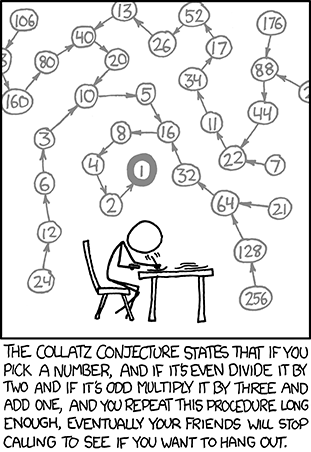
\includegraphics[height=2in]{prologue/pix/collatz_conjecture.png}  \\
  \caption{\href{https://xkcd.com/710/}{由 \texttt{xkcd.com} 提供}}
  \label{fig:XKCDCollatz}
\end{figure}
\end{exparts}
\end{answer}
\end{exercise}

\begin{exercise}
\begin{credit}
  SE user Ted, https://math.stackexchange.com/a/75300/12012 
\end{credit}
Ackermann 函数在直觉上是可机械计算的（并且是全函数），但它不是原始递归的。
下面给出另一个这样的函数。
% (It uses a technique from the next chapter called `diagonalization'.)
假设所有偏递归函数都接受一个自然数输入，并产生一个自然数输出。
（我们可以用 G\"{o}del 乘法编码模拟输入对等；参见\zcref{exer:CourseOfValuesRecursion}。）
令 $f_0$, $f_1$, \ldots{} 是所有原始递归函数的一个有效列表。
也就是说，存在一个原始递归函数，它输入索引~$i$，返回某种计算~$f_i$ 的方式。
（\textit{注：}~这相当于一个原始递归函数的解释器，给定函数的描述~$i$，就能对任意输入~$x$ 计算 $f_i(x)$。）
现在考虑函数$D(n)=f_n(n)+1$。
证明 $D$ 虽然直觉上可计算，但不是原始递归的。
\begin{answer}\verified
如果 $D$ 是原始递归的，那么它就是某个~$f_i$。
但这样一来$D(i)=f_i(i)+1=D(i)+1$，这是不可能的。  
\end{answer}
\end{exercise}

\end{exercises}
\index{general recursion|)}\index{recursion|)}

% ==================================
\extra{Turing 机模拟器}\index{Turing machine!simulator|(} \label{extra:TuringMachineSimilator}

本书的源代码仓库中包含一个用 Racket 编写的程序，用于模拟 Turing 机。
它位于目录
\lstinline{src/scheme/prologue}。
这里我们将展示如何运行这个模拟器。
（其实现紧密遵循
书中第~\pageref{DefnConfiguration}页对 Turing 机动作的描述。）

\zcref{ex:MPred}给出了一个计算
前驱函数的 Turing 机。
\begin{equation*}
 \TM_{\text{pred}}=
  \set{ \tminstruction{0}{B}{L}{1},\,
        \tminstruction{0}{1}{R}{0},\,
        \tminstruction{1}{B}{L}{2},\,
        \tminstruction{1}{1}{B}{1},\,
        \tminstruction{2}{B}{R}{3},\,
        \tminstruction{2}{1}{L}{2} 
      }
\end{equation*}
它对应于输入文件 \lstinline{pred.tm}。
\lstinputlisting{\tmfiles pred.tm}
因此，任何一个特定 Turing 机的模拟器实际上由两部分组成：
Racket 代码和机器的描述文件，如上所示。

下面是模拟器的一次运行，包括其命令行调用。
机器启动时的当前符号为 \str{1}，
当前符号右侧的纸带内容为 \str{11}（左侧的纸带为空）。
因此，整个纸带输入是 $\tau=\str{111}$。
因为 $3$ 的前驱是~$2$，我们期望结束时纸带会包含 \str{11}，其余部分为空白。
\begin{lstlisting} 
computing/src/scheme/prologue$ ./turing-machine.rkt -f machines/pred.tm -c "1" -r "11"
step 0: q0: *1*11
step 1: q0: 1*1*1
step 2: q0: 11*1*
step 3: q0: 111*B*
step 4: q1: 11*1*B
step 5: q1: 11*B*B
step 6: q2: 1*1*BB
step 7: q2: *1*1BB
step 8: q2: *B*11BB
step 9: q3: B*1*1BB
step 10: HALT
\end{lstlisting}  % $
输出虽然粗陋，但对于小实验来说已经足够。
命令行 \lstinline{turing-machine.rkt --help} 可以查看
模拟器的选项。

\begin{exercises}


\begin{exercise}
使用模拟器运行 $\TM_{\text{pred}}$，初始输入为 \str{11111}。
同时也以空纸带启动。
\begin{answer}
以下是以五个 \str{1} 作为初始输入的命令行运行记录。
\begin{lstlisting}
$ ./turing-machine.rkt -f machines/pred.tm -c "1" -r "1111"
step 0: q0: *1*1111
step 1: q0: 1*1*111
step 2: q0: 11*1*11
step 3: q0: 111*1*1
step 4: q0: 1111*1*
step 5: q0: 11111*B*
step 6: q1: 1111*1*B
step 7: q1: 1111*B*B
step 8: q2: 111*1*BB
step 9: q2: 11*1*1BB
step 10: q2: 1*1*11BB
step 11: q2: *1*111BB
step 12: q2: *B*1111BB
step 13: q3: B*1*111BB
step 14: HALT
\end{lstlisting}  % $
以下是其纸带图格式。
\begin{tapesequence}
  \begin{tapesequencetable}
    0 &\tapegraphic{\tmexercises pred_five000.pdf} \\
    1 &\tapegraphic{\tmexercises pred_five001.pdf} \\
    2 &\tapegraphic{\tmexercises pred_five002.pdf} \\
    3 &\tapegraphic{\tmexercises pred_five003.pdf} \\
    4 &\tapegraphic{\tmexercises pred_five004.pdf} \\
  \end{tapesequencetable}
  \hspace*{2em}
  \begin{tapesequencetable}
    5 &\tapegraphic{\tmexercises pred_five005.pdf} \\
    6 &\tapegraphic{\tmexercises pred_five006.pdf} \\
    7 &\tapegraphic{\tmexercises pred_five007.pdf} \\
    8 &\tapegraphic{\tmexercises pred_five008.pdf} \\
    9 &\tapegraphic{\tmexercises pred_five009.pdf} \\
  \end{tapesequencetable}
  \hspace*{2em}
  \begin{tapesequencetable}
   10 &\tapegraphic{\tmexercises pred_five010.pdf} \\
   11 &\tapegraphic{\tmexercises pred_five011.pdf} \\
   12 &\tapegraphic{\tmexercises pred_five012.pdf} \\
   13 &\tapegraphic{\tmexercises pred_five013.pdf} \\
  \end{tapesequencetable}
\end{tapesequence}
这是以空纸带作为初始输入的命令行调用，
\begin{lstlisting}
$ ./turing-machine.rkt -f machines/pred.tm -c " "
step 0: q0: *B*
step 1: q1: *B*B
step 2: q2: *B*BB
step 3: q3: B*B*B
step 4: HALT
\end{lstlisting}  % $
以及对应的纸带图序列。
\begin{tapesequence}
  \begin{tapesequencetable}
    0 &\tapegraphic{\tmexercises pred_empty000.pdf} \\
    1 &\tapegraphic{\tmexercises pred_empty001.pdf} \\
    2 &\tapegraphic{\tmexercises pred_empty002.pdf} \\
    3 &\tapegraphic{\tmexercises pred_empty003.pdf} \\
  \end{tapesequencetable}
\end{tapesequence}
\end{answer}
\end{exercise}

\begin{exercise}
在例~\ref{ex:MAdd}的加法 Turing 机 $\TM_{\text{add}}$ 上运行模拟器来计算 $1+2$。
同时模拟 $0+2$ 和 $0+0$。
\begin{answer}
这模拟了 $1+2$。
\begin{lstlisting}
$ ./turing-machine.rkt -f machines/pred.tm -c "1" -r " 11"
step 0: q0: *1* 11
step 1: q0: 1*B*11
step 2: q1: 1*B*11
step 3: q1: 1*1*11
step 4: q2: 1*1*11
step 5: q2: *1*111
step 6: q2: *B*1111
step 7: q3: *B*1111
step 8: q3: B*1*111
step 9: q4: B*B*111
step 10: q5: BB*1*11
step 11: HALT
\end{lstlisting}  % $
这是对应的纸带图。
\begin{tapesequence}
  \begin{tapesequencetable}
    0 &\tapegraphic{\tmexercises addonetwo000.pdf} \\
    1 &\tapegraphic{\tmexercises addonetwo001.pdf} \\
    2 &\tapegraphic{\tmexercises addonetwo002.pdf} \\
    3 &\tapegraphic{\tmexercises addonetwo003.pdf} \\
  \end{tapesequencetable}
  \hspace*{2em}
  \begin{tapesequencetable}
    4 &\tapegraphic{\tmexercises addonetwo004.pdf} \\
    5 &\tapegraphic{\tmexercises addonetwo005.pdf} \\
    6 &\tapegraphic{\tmexercises addonetwo006.pdf} \\
    7 &\tapegraphic{\tmexercises addonetwo007.pdf} \\
  \end{tapesequencetable}
  \hspace*{2em}
  \begin{tapesequencetable}
    8 &\tapegraphic{\tmexercises addonetwo008.pdf} \\
    9 &\tapegraphic{\tmexercises addonetwo009.pdf} \\
   10 &\tapegraphic{\tmexercises addonetwo010.pdf} \\
  \end{tapesequencetable}
\end{tapesequence}
$0+2$ 的命令行
\begin{lstlisting}
$ ./turing-machine.rkt -f machines/pred.tm -c " " -r "11"
\end{lstlisting}  % $
给出这些纸带图。
\begin{tapesequence}
  \begin{tapesequencetable}
    0 &\tapegraphic{\tmexercises addzerotwo000.pdf} \\
    1 &\tapegraphic{\tmexercises addzerotwo001.pdf} \\
    2 &\tapegraphic{\tmexercises addzerotwo002.pdf} \\
  \end{tapesequencetable}
  \hspace*{2em}
  \begin{tapesequencetable}
    3 &\tapegraphic{\tmexercises addzerotwo003.pdf} \\
    4 &\tapegraphic{\tmexercises addzerotwo004.pdf} \\
    5 &\tapegraphic{\tmexercises addzerotwo005.pdf} \\
  \end{tapesequencetable}
  \hspace*{2em}
  \begin{tapesequencetable}
    6 &\tapegraphic{\tmexercises addzerotwo006.pdf} \\
    7 &\tapegraphic{\tmexercises addzerotwo007.pdf} \\
    8 &\tapegraphic{\tmexercises addzerotwo008.pdf} \\
  \end{tapesequencetable}
\end{tapesequence}
$0+0$ 的命令行
\begin{lstlisting}
$ ./turing-machine.rkt -f machines/pred.tm -c " " 
\end{lstlisting}  % $
给出了以下纸带图序列。
\begin{tapesequence}
  \begin{tapesequencetable}
    0 &\tapegraphic{\tmexercises addzerozero000.pdf} \\
    1 &\tapegraphic{\tmexercises addzerozero001.pdf} \\
    2 &\tapegraphic{\tmexercises addzerozero002.pdf} \\
  \end{tapesequencetable}
  \hspace*{2em}
  \begin{tapesequencetable}
    3 &\tapegraphic{\tmexercises addzerozero003.pdf} \\
    4 &\tapegraphic{\tmexercises addzerozero004.pdf} \\
    5 &\tapegraphic{\tmexercises addzerozero005.pdf} \\
  \end{tapesequencetable}
  \hspace*{2em}
  \begin{tapesequencetable}
    6 &\tapegraphic{\tmexercises addzerozero006.pdf} \\
    7 &\tapegraphic{\tmexercises addzerozero007.pdf} \\
    8 &\tapegraphic{\tmexercises addzerozero008.pdf} \\
  \end{tapesequencetable}
\end{tapesequence}
\end{answer}
\end{exercise}

\begin{exercise}
编写一个 Turing 机来执行加~$3$ 的操作，
使得给定一个仅包含连续 $n$ 个 \str{1} 的串的纸带作为输入时，它返回一个包含连续 $n+3$ 个 \str{1} 的串的纸带。
遵循我们的约定：程序启动和结束时，读写头都位于第一个 \str{1} 的下方。
在模拟器上运行它，输入分别为 $4$ 个连续的 \str{1}，以及空纸带。
\begin{answer}
这个十条指令的机器
\begin{align*}
  \TM_{\text{addthree}} 
  &=
  \{\hspace{\setspacing} \tminstruction{0}{1}{R}{0},\,
        \tminstruction{0}{B}{B}{1},\,
        \tminstruction{1}{B}{1}{1},\,
        \tminstruction{1}{1}{R}{2},\,
        \tminstruction{2}{B}{1}{2},\,
        \tminstruction{2}{1}{R}{3},\,        \\
        &\qquad\;\tminstruction{3}{B}{1}{3},\,
        \tminstruction{3}{1}{1}{4},\,          
        \tminstruction{4}{1}{L}{4},\,
        \tminstruction{4}{B}{R}{5} 
      \hspace{\setspacing}\}
\end{align*}
\noindent 与模拟器的源文件一致。
\lstinputlisting{\tmfiles addthree.tm}
\noindent 输入为~$4$ 的命令行
\begin{lstlisting}
$ ./turing-machine.rkt -f machines/addthree.tm -c "1" -r "111"
\end{lstlisting}  % $
\noindent 给出了以下纸带图。
\begin{tapesequence}
  \begin{tapesequencetable}
    0  &\tapegraphic{\tmexercises addthree_four000.pdf} \\
    1  &\tapegraphic{\tmexercises addthree_four001.pdf} \\
    2  &\tapegraphic{\tmexercises addthree_four002.pdf} \\
    3  &\tapegraphic{\tmexercises addthree_four003.pdf} \\
    4  &\tapegraphic{\tmexercises addthree_four004.pdf} \\
    5  &\tapegraphic{\tmexercises addthree_four005.pdf} \\
    6  &\tapegraphic{\tmexercises addthree_four006.pdf} \\
  \end{tapesequencetable}
  \hspace*{2em}
  \begin{tapesequencetable}
    7  &\tapegraphic{\tmexercises addthree_four007.pdf} \\
    8  &\tapegraphic{\tmexercises addthree_four008.pdf} \\
    9  &\tapegraphic{\tmexercises addthree_four009.pdf} \\
   10  &\tapegraphic{\tmexercises addthree_four010.pdf} \\
   11  &\tapegraphic{\tmexercises addthree_four011.pdf} \\
   12  &\tapegraphic{\tmexercises addthree_four012.pdf} \\
   13  &\tapegraphic{\tmexercises addthree_four013.pdf} \\
  \end{tapesequencetable}
  \hspace*{2em}
  \begin{tapesequencetable}
   14  &\tapegraphic{\tmexercises addthree_four014.pdf} \\
   15  &\tapegraphic{\tmexercises addthree_four015.pdf} \\
   16  &\tapegraphic{\tmexercises addthree_four016.pdf} \\
   17  &\tapegraphic{\tmexercises addthree_four017.pdf} \\
   18  &\tapegraphic{\tmexercises addthree_four018.pdf} \\
   19  &\tapegraphic{\tmexercises addthree_four019.pdf} \\
  \end{tapesequencetable}
\end{tapesequence}
输入为 $0$ 的命令行
\begin{lstlisting}
$ ./turing-machine.rkt -f machines/addthree.tm -c " " 
\end{lstlisting}  % $
\noindent 给出了以下纸带图序列。
\begin{tapesequence}
  \begin{tapesequencetable}
    0  &\tapegraphic{\tmexercises addthree_zero000.pdf} \\
    1  &\tapegraphic{\tmexercises addthree_zero001.pdf} \\
    2  &\tapegraphic{\tmexercises addthree_zero002.pdf} \\
    3  &\tapegraphic{\tmexercises addthree_zero003.pdf} \\
  \end{tapesequencetable}
  \hspace*{2em}
  \begin{tapesequencetable}
    4  &\tapegraphic{\tmexercises addthree_zero004.pdf} \\
    5  &\tapegraphic{\tmexercises addthree_zero005.pdf} \\
    6  &\tapegraphic{\tmexercises addthree_zero006.pdf} \\
    7  &\tapegraphic{\tmexercises addthree_zero007.pdf} \\
  \end{tapesequencetable}
  \hspace*{2em}
  \begin{tapesequencetable}
    8  &\tapegraphic{\tmexercises addthree_zero008.pdf} \\
    9  &\tapegraphic{\tmexercises addthree_zero009.pdf} \\
   10  &\tapegraphic{\tmexercises addthree_zero010.pdf} \\
   11  &\tapegraphic{\tmexercises addthree_zero011.pdf} \\
  \end{tapesequencetable}
\end{tapesequence}
\end{answer}
\end{exercise}

\begin{exercise}
编写一台机器来判定输入是否包含子串~\str{010}。
固定 $\Sigma=\set{\str{0}, \str{1}, \str{B}}$。
机器初始时，纸带上除了一串连续的 \str{0} 和 \str{1} 外全是空白，
且读写头位于第一个非空白符号下方。
结束时，如果输入包含所需的子串，则纸带上将只有一个~\str{1}；
否则只有一个~\str{0}。
我们将分阶段进行，构建几个相当于子程序的部分。
\begin{exparts}
\item 编写从状态~$q_{10}$ 开始的指令，使得如果初始时机器的读写头位于一串非空白符号的首个上方，那么结束时读写头将处于最后一个此类符号的右侧。
\item 编写从状态~$q_{20}$ 开始的一系列指令，使得如果初始时读写头紧邻一串非空白符号的右侧，那么结束时所有这些符号都变为空白。
\item 编写完整的机器，包括将前面的项连接起来。
\end{exparts}
\begin{answer}
\begin{exparts}
\item
像下面这样就可以了。
\begin{equation*}
  \TM_0=\set{\tminstruction{10}{0}{R}{10},\,
       \tminstruction{10}{1}{R}{10},\,
       \tminstruction{10}{B}{B}{100} }
\end{equation*}
\item
这会向后移动，将格子擦除为空白。
\begin{equation*}
  \TM_1=\set{ 
       \tminstruction{20}{0}{B}{21},\,
       \tminstruction{20}{1}{B}{21},\,
       \tminstruction{20}{B}{B}{100},\,   
       \tminstruction{21}{0}{L}{20},\,
       \tminstruction{21}{1}{L}{20},\,
       \tminstruction{21}{B}{L}{20} 
      }
\end{equation*}
\item 这里，粗略地说，$q_0$ 表示尚未匹配到子串的任何部分，
$q_1$ 表示已看到 \str{0}，机器正在寻找~\str{1}，
而~$q_2$ 表示已看到 \str{01}，机器正在寻找~\str{0}。
接着，四个状态 $q_3$、$q_4$、$q_5$ 和 $q_6$ 表示失败
（它们以 $q_6$ 在空白纸带上写入~\str{0} 而结束）。
四个状态 $q_7$、$q_8$、$q_9$ 和 $q_{10}$ 表示成功。
\begin{align*}
  \TM_{\text{decide010}} 
  &=
  \{\hspace{\setspacing} \tminstruction{0}{0}{R}{1},\,
        \tminstruction{0}{1}{R}{0},\,
        \tminstruction{0}{B}{B}{3},\,
        \tminstruction{1}{0}{R}{1},\,
        \tminstruction{1}{1}{R}{2},\,
        \tminstruction{1}{B}{B}{3},\,        
        \tminstruction{2}{0}{R}{7},\,
        \tminstruction{2}{1}{1}{0},\,
        \tminstruction{2}{B}{B}{3},\,        \\
        &\qquad\;
        \tminstruction{3}{0}{R}{3},\,
        \tminstruction{3}{1}{R}{3},\,          
        \tminstruction{3}{B}{L}{4},\,
        \tminstruction{4}{0}{B}{5},\,
        \tminstruction{4}{1}{B}{5},\,       
        \tminstruction{4}{B}{B}{6},\,   \\  % too big to fit on one line
        &\qquad\qquad\tminstruction{5}{0}{L}{4},\,
        \tminstruction{5}{1}{L}{4},\,          
        \tminstruction{5}{B}{L}{4},\,
        \tminstruction{6}{0}{0}{100},\,
        \tminstruction{6}{1}{0}{100},\,          
        \tminstruction{6}{B}{0}{100},\,      \\
        &\qquad\;
        \tminstruction{7}{0}{R}{7},\,
        \tminstruction{7}{1}{R}{7},\,          
        \tminstruction{7}{B}{L}{8},\,
        \tminstruction{8}{0}{B}{9},\,
        \tminstruction{8}{1}{B}{9},\,          
        \tminstruction{8}{B}{B}{10},\,      \\  % too big
        &\qquad\qquad\tminstruction{9}{0}{L}{8},\,
        \tminstruction{9}{1}{L}{8},\,          
        \tminstruction{9}{B}{L}{8},\,
        \tminstruction{10}{0}{1}{100},\,
        \tminstruction{10}{1}{1}{100},\,          
        \tminstruction{10}{B}{1}{100}      
      \hspace{\setspacing}\}
\end{align*}
\end{exparts}
\end{answer}
\end{exercise}

% Write a Turing machine to perform the proper subtraction
% operation on two inputs, often denoted $x\dotminus y$,
% that yields $x-y$ if $x\geq y$ and~$0$ otherwise. 
% Run it on the simulator to compute $5\dotminus 3$ and $3\dotminus 5$.

% \begin{exercise}
% Modify the simulator so that it can run for a limited number of steps.
% \begin{exparts}
% \item Modify it so that, given~$k\in\N$, if the Turing machine hasn't halted
% after $k$ steps then the simulator stops.
% \item Do the same, but replace $k$ with a function \codeinline{(k n)} where
% \str{n} is the input number (assume the machine's input is a string
% of \str{1}'s). 
% \end{exparts}
% \end{exercise}

\end{exercises}
\index{Turing machine!simulator|)}

% ==================================
\extra{硬件}  \label{extra:Hardware}
遵循 Turing 的方法，我们已经基于转移构建了关于“什么是可计算的”的定义。
我们生成一个转移指令表，并将其称为一台机器。
但是，我们能否确定每个转移表都有一个对应的实际机制，
即一个具有该行为的物理实现呢？

换个说法，在编程语言中，存在由其他更简单的运算符构造而成的运算符。
例如，\citetext{$\sin(x)$ 可以通过其 Taylor 多项式计算}{%
  Taylor 级数是 $\sin(x)=x-x^3/3!+x^5/5!-x^7/7!+\cdots$。
  我们可以通过决定在 $x^5$ 项截断该级数来得到一个 Taylor 多项式，从而进行实际计算。} 的值可由加法和乘法计算得出。
但是，最基本的操作必须在硬件层面发生；它们是如何实现的呢？

我们将展示如何从任何期望的行为出发，构造出相应的设备。
为此，我们将处理以比特串作为输入和输出的机器。
最简单的方法是通过命题逻辑。
（\zcref{sec:PropLogic}处有相关回顾。）

以下是三个基本的逻辑运算符。
这些表格用 $0$ 替代~$F$，用 $1$ 替代~$T\!$，这是电子学中的惯例。


\begin{center}\small % \vspace{0.5ex}
  \begin{tabular}[t]{c|c}
    \multicolumn{1}{c}{\ }    
        &\multicolumn{1}{c}{\tabulartext{非}$P$}  \\[-0.25ex]
    \multicolumn{1}{c}{$P$}      
        &\multicolumn{1}{c}{$\neg P$}  \\
    \hline
       $0$  &$1$  \\
       $1$  &$0$
  \end{tabular}
  \qquad
  \begin{tabular}[t]{cc|cc}
    \multicolumn{1}{c}{\ }    
        &\multicolumn{1}{c}{\ }    
        &\multicolumn{1}{c}{$P$ \tabulartext{与} $Q$}  
        &\multicolumn{1}{c}{$P$ \tabulartext{或} $Q$}  \\[-0.25ex]
    \multicolumn{1}{c}{$P$}      
        &\multicolumn{1}{c}{$Q$}      
        &\multicolumn{1}{c}{$P\wedge Q$}  
        &\multicolumn{1}{c}{$P\vee Q$}  \\
    \hline
       $0$  &$0$  &$0$  &$0$  \\
       $0$  &$1$  &$0$  &$1$  \\
       $1$  &$0$  &$0$  &$1$  \\
       $1$  &$1$  &$1$  &$1$  
  \end{tabular}
\end{center}

这三个逻辑运算符就是我们所需的全部。
我们将展示如何从一个指定的输入-输出行为，即一个期望的真值表，
得到一个仅使用“$\neg$”、“$\wedge$”和“$\vee$”并具有该行为的命题逻辑表达式。
然后我们将概述如何用电子元件实现它。

下面的两个表格展示了具体做法。
从左边那个表格开始，关注输出为~$1$ 的那一行。
表达式 $\neg P\wedge \neg Q$
使这一行的值为~$1$，而其他所有行的值为~$0$。


\begin{center} \small
  \begin{tabular}[t]{cc|c}
    \multicolumn{1}{c}{$P$}      
        &\multicolumn{1}{c}{$Q$}      
        &\multicolumn{1}{c}{}  \\
    \hline
       $0$  &$0$  &$1$  \\
       $0$  &$1$  &$0$  \\
       $1$  &$0$  &$0$  \\
       $1$  &$1$  &$0$  
  \end{tabular}
  \hspace{3em}
  \begin{tabular}[t]{ccc|c}
    \multicolumn{1}{c}{$P$}
    &\multicolumn{1}{c}{$Q$}
    &\multicolumn{1}{c}{$R$}
    &\multicolumn{1}{c}{}     \\ \hline
    $0$  &$0$  &$0$  &$0$    \\
    $0$  &$0$  &$1$  &$1$    \\
    $0$  &$1$  &$0$  &$1$    \\
    $0$  &$1$  &$1$  &$0$    \\[.5ex]
    $1$  &$0$  &$0$  &$1$    \\
    $1$  &$0$  &$1$  &$0$    \\
    $1$  &$1$  &$0$  &$0$    \\
    $1$  &$1$  &$1$  &$0$    
  \end{tabular}  
\end{center}


对于右边的表格，同样关注输出为~$1$ 的那些行。
第二行对应的子句是 $\neg P\wedge \neg Q\wedge R$。
针对第三行，使用 $\neg P\wedge Q\wedge \neg R$；
针对第五行，使用 $P\wedge\neg Q\wedge\neg R$。
现在用 $\vee$ 将这些子句组合起来，就得到了符合给定真值表的命题。
（由使用 $\wedge$ 的子句并通过 $\vee$ 连接而成的命题，称为析取范式（DNF）。
参见\zcref{sec:PropLogic}。）\index{Disjunctive Normal form, DNF}\index{DNF}\index{Propositional logic!Disjunctive Normal form}
\begin{equation*}
(\neg P\wedge \neg Q\wedge R)
  \vee(\neg P\wedge Q\wedge \neg R)
  \vee(P\wedge\neg Q\wedge\neg R)
\tag{$*$}
\end{equation*}

\margingraphic{0.22\textwidth}{prologue/pix/shannon.jpg}{\label{fig:shannon}\href{https://en.wikipedia.org/wiki/Claude_Shannon}{Claude Shannon 1916--2001}}\index{Shannon, C!picture}
% See also http://nautil.us/issue/51/limits/how-information-got-re_invented
接下来，我们将这些表达式转化为器件。
利用这种形式的命题逻辑表达式来系统地设计逻辑电路，这一发现是由\citetext{C~Shannon}{参见他的个人简介：\protect\url{http://www.newyorker.com/tech/elements/claude-shannon-the-father-of-the-information-age-turns-1100100}.} 在其 1937 年的\citetext{硕士论文}{%
他的相关论文就是他的硕士论文，\protect\url{https://en.wikipedia.org/wiki/A_Symbolic_Analysis_of_Relay_and_Switching_Circuits}.} 中提出的。
我们可以获得被称为
\definend{门}的电子器件，\index{gate}\index{logic gate}
它能对信号执行逻辑操作。
（在本讨论中，我们将出现 $5$ 伏特电压视为信号 $1$，$0$ 伏特视为信号 $0$）。
下方左侧是一个具有两根输入导线和一根输出导线的
\textsc{与}门的电路符号，其行为是：只有当两个输入端都有信号时，输出端才会有信号。
中间所画的是一个 \textsc{或}门的符号，只要任一输入端有信号，输出端就有信号。
右侧是一个 \textsc{非}门的符号。


\begin{center}
  \vcenteredhbox{\includegraphics{prologue/asy/gates/gates00.pdf}}
  \qquad
  \vcenteredhbox{\includegraphics{prologue/asy/gates/gates01.pdf}}
  \qquad
  \vcenteredhbox{\includegraphics{prologue/asy/gates/gates02.pdf}}
\end{center}

下方给出了实现表达式~($*$) 的电路示意图，左侧的三条导线表示三个输入信号。
例如，为了实现第一个子句，顶部的 \textsc{与}门接收非~$P$、非~$Q$ 和~$R$ 信号。
第二和第三个子句由另外两个 \textsc{与}门实现。
然后，\textsc{与}门的输出被送入 \textsc{或}门。
（这些 \textsc{与}门和 \textsc{或}门被设计为能接收三个输入；我们不必在意市面上实际出售的是哪些类型的这种器件。）


\begin{center}
  \includegraphics{prologue/asy/gates/gates03.pdf}
\end{center}

显然，遵循这一步骤，我们原则上可以构建出具有任何期望输入/输出行为的物理设备。
特别地，我们可以通过这种方式构建一台 Turing 机。

最后，我们稍作题外探讨。
有人可能会好奇这些门是如何构造的，特别是会好奇一个 \textsc{非}门怎么可能存在——输入端没有电压时输出端却有电压，这不是无中生有吗？

答案是，上述描述抽象掉了一些细节。
这里展示了一种
\citetext{\textsc{非}门}{%
这是 N 型金属氧化物半导体晶体管的一种。还有许多其他类型。}
的内部构造。


\begin{center}
  \includegraphics{prologue/asy/gates/gates04.pdf}
\end{center}


右边是一个电池，正如我们将要看到的，它提供了额外的电压。
左上角画成波浪线的是电阻。当电流流经电路时，该电阻会调节来自电池的功率输出。

左下角带有圆圈的是晶体管。如果在~\textsf{G} 和~\textsf{S} 之间有足够的电压，该元件就会允许来自电池的电流在 \textsf{D} 和 \textsf{S} 之间流动。
（因为它有时断开有时闭合，所以被画作开关，尽管它并没有活动部件。）
这种晶体管在制造时设定为，$5$ 伏特的输入电压~$V_{\text{in}}$ 即可触发这一动作。

为了验证该电路对信号取反，首先假设 $V_{\text{in}}=0$。
那么，\textsf{D} 和~\textsf{S} 之间没有电流流动。
由于没有电流，电阻不会产生电压降，因此间隙两端的输出电压~$V_{\text{out}}$ 等于电池提供的全部电压，即 $5$ 伏特。
所以，$V_{\text{in}}=0$ 使得~$V_{\text{out}}=5$。

反之，假设 $V_{\text{in}}=5$。
那么电流在 \textsf{D} 和~\textsf{S} 之间流动，电阻因此产生电压降，这意味着输出为~$V_{\text{out}}=0$。

因此，对于这个器件，输出电压 $V_{\text{out}}$ 与输入电压~$V_{\text{in}}$ 相反。
% When $V_{\text{in}}=0$ the output voltage of~$5$ doesn't come from 
% nowhere;~it comes from the battery.

\begin{exercises}

\begin{exercise}
一个常用的命题逻辑运算符是
\definend{异或（\textsc{XOR}）}。\index{exclusive or@exclusive or \textsc{XOR}}\index{XOR@\textsc{XOR}, exclusive or}\index{Propositional logic!exclusive or@exclusive or \textsc{XOR}}
其定义为：$P\mathbin{\textsc{XOR}}Q=1$ 为 $1$ 当且仅当 $P\neq Q$。
\begin{exparts}
\item 列出真值表，并根据它构造一个析取范式（DNF）命题逻辑表达式。
\item 用该表达式设计一个回路。
\end{exparts}
\begin{answer}\verified
\begin{exparts}
\item 真值表如下。
\begin{display}
  \begin{tabular}[t]{cc|c}
    \multicolumn{1}{c}{$P$}      
        &\multicolumn{1}{c}{$Q$}      
        &\multicolumn{1}{c}{$P\mathbin{\textsc{XOR}}Q$}  \\
    \hline
       $0$  &$0$  &$0$  \\
       $0$  &$1$  &$1$  \\
       $1$  &$0$  &$1$  \\
       $1$  &$1$  &$0$  
  \end{tabular}    
\end{display}
表达式为$(\neg P\wedge \neg Q)
  \vee(P\wedge Q)$。
\item  $P\mathbin{\textsc{XOR}}Q$ 的回路如图\figureref{fig:PxorQCircuit}所示。
\begin{figure} 
  \centering
  \includegraphics{prologue/asy/gates/gates06.pdf}  \\
  \caption{$P\mathbin{\textsc{XOR}}Q$ 的回路。}
  \label{fig:PxorQCircuit}
\end{figure}
\end{exparts}
\end{answer}
\end{exercise}

\begin{exercise}
命题逻辑运算符
\definend{蕴含}（\definend{$\rightarrow$}）\index{Propositional logic!implication}\index{implication logic operator $\rightarrow$}
定义为：除了 $P$ 为 $1$ 且 $Q$ 为 $0$ 的情况外，$P\rightarrow Q$ 均为 $1$。
\begin{exparts}
\item 列出真值表，并根据它构造一个析取范式表达式。
\item 用该表达式设计一个回路。
\end{exparts}
\begin{answer}\verified
\begin{exparts}
\item 根据定义，输入/输出行为如下：
\begin{display} \small
  \begin{tabular}[t]{cc|c}
    \multicolumn{1}{c}{$P$}
    &\multicolumn{1}{c}{$Q$}
    &\multicolumn{1}{c}{$P\rightarrow Q$}     \\ \hline
    $0$  &$0$  &$1$    \\
    $0$  &$1$  &$1$    \\
    $1$  &$0$  &$0$    \\
    $1$  &$1$  &$1$    
  \end{tabular}  
\end{display}
因此，布尔表达式为
$(\neg P\wedge \neg Q)
  \vee(\neg P\wedge Q)
  \vee(P\wedge Q)$。
\item 蕴含运算的回路如图\figureref{fig:ImpliesCircuit}所示。
\begin{figure} 
  \centering
  \includegraphics{prologue/asy/gates/gates11.pdf}  \\
  \caption{蕴含运算的回路。}
  \label{fig:ImpliesCircuit}
\end{figure}
\end{exparts}
\end{answer}
\end{exercise}

\begin{exercise}
根据下表构造一个析取范式命题逻辑表达式。
\begin{center} \small
  \begin{tabular}[t]{cc|c}
    \multicolumn{1}{c}{$P$}
    &\multicolumn{1}{c}{$Q$}
    &\multicolumn{1}{c}{}     \\ \hline
    $0$  &$0$  &$0$    \\
    $0$  &$1$  &$1$    \\
    $1$  &$0$  &$0$    \\
    $1$  &$1$  &$1$    
  \end{tabular}  
\end{center}
用该表达式设计一个回路。
\begin{answer}\verified
表达式为$(\neg P\wedge Q)
  \vee(P\wedge Q)$。
回路如图\figureref{fig:QCircuit}所示。
\begin{figure} 
  \centering
  \includegraphics{prologue/asy/gates/gates08.pdf}  \\
  \caption{未命名运算的回路（不妨称之为 $Q$）。}
  \label{fig:QCircuit}
\end{figure}
\end{answer}
\end{exercise}

\begin{exercise}
为下表各构造一个析取范式命题逻辑表达式。
\begin{center} \small
  \begin{tabular}[t]{ccc|c}
    \multicolumn{1}{c}{$P$}
    &\multicolumn{1}{c}{$Q$}
    &\multicolumn{1}{c}{$R$}
    &\multicolumn{1}{c}{}     \\ \hline
    $0$  &$0$  &$0$  &$0$    \\
    $0$  &$0$  &$1$  &$1$    \\
    $0$  &$1$  &$0$  &$1$    \\
    $0$  &$1$  &$1$  &$0$    \\[.5ex]
    $1$  &$0$  &$0$  &$0$    \\
    $1$  &$0$  &$1$  &$1$    \\
    $1$  &$1$  &$0$  &$0$    \\
    $1$  &$1$  &$1$  &$0$    
  \end{tabular}  
  \qquad
  \begin{tabular}[t]{ccc|c}
    \multicolumn{1}{c}{$P$}
    &\multicolumn{1}{c}{$Q$}
    &\multicolumn{1}{c}{$R$}
    &\multicolumn{1}{c}{}     \\ \hline
    $0$  &$0$  &$0$  &$1$    \\
    $0$  &$0$  &$1$  &$0$    \\
    $0$  &$1$  &$0$  &$1$    \\
    $0$  &$1$  &$1$  &$0$    \\[.5ex]
    $1$  &$0$  &$0$  &$0$    \\
    $1$  &$0$  &$1$  &$0$    \\
    $1$  &$1$  &$0$  &$1$    \\
    $1$  &$1$  &$1$  &$1$    
  \end{tabular}  
\end{center}
用这些表达式设计回路：
\begin{exparts}
\item 左表；
\item 右表。
\end{exparts}
\begin{answer}\verified
两个回路如图\figureref{fig:BothTableCircuits}所示。
\begin{figure} 
  \centering
  \vcenteredhbox{\includegraphics{prologue/asy/gates/gates09.pdf}}  
  \qquad
  \vcenteredhbox{\includegraphics{prologue/asy/gates/gates10.pdf}}  \\
  \caption{两个未命名运算表的回路。}
  \label{fig:BothTableCircuits}
\end{figure}
\begin{exparts}
\item 在表达式中，每个子句对应输出为 $1$ 的一行。
\begin{equation*}
(\neg P\wedge \neg Q\wedge R)
  \vee(\neg P\wedge Q\wedge \neg R)
  \vee(P\wedge \neg Q\wedge R)
\end{equation*}
\item 子句对应输出为 $1$ 的行。
\begin{equation*}
(\neg P\wedge \neg Q\wedge \neg R)
  \vee(\neg P\wedge Q\wedge \neg R)
  \vee(P\wedge Q\wedge \neg R)
  \vee(P\wedge Q\wedge R).
\end{equation*}
\end{exparts}
\end{answer}
\end{exercise}

\begin{exercise}
针对“若 $P$ 等于 $R$ 则输出为 $1$”的行为，制作一个以 $P$、$Q$ 和 $R$ 为输入的真值表。
写出对应的析取范式（DNF）表达式。
画出回路图。
\begin{answer}\verified
输入/输出行为如下：
\begin{display}
  \begin{tabular}[t]{ccc|c}
    \multicolumn{1}{c}{$P$}
    &\multicolumn{1}{c}{$Q$}
    &\multicolumn{1}{c}{$R$}
    &\multicolumn{1}{c}{}     \\ \hline
    $0$  &$0$  &$0$  &$1$    \\
    $0$  &$0$  &$1$  &$0$    \\
    $0$  &$1$  &$0$  &$1$    \\
    $0$  &$1$  &$1$  &$0$    \\[.5ex]
    $1$  &$0$  &$0$  &$0$    \\
    $1$  &$0$  &$1$  &$1$    \\
    $1$  &$1$  &$0$  &$0$    \\
    $1$  &$1$  &$1$  &$1$    
  \end{tabular}  
\end{display}
该表直接给出了析取范式（DNF）表达式：
\begin{equation*}
(\neg P\wedge \neg Q\wedge \neg R)
  \vee(\neg P\wedge Q\wedge \neg R)
  \vee(P\wedge\neg Q\wedge R)
  \vee(P\wedge Q\wedge R)
\end{equation*}
回路如图\figureref{fig:PEqualsRCircuit}所示。
\begin{figure} 
  \centering
  \includegraphics{prologue/asy/gates/gates05.pdf}  \\
  \caption{$P=R$ 的回路。}
  \label{fig:PEqualsRCircuit}
\end{figure}
\end{answer}
\end{exercise}

\begin{exercise}
针对“多数输入为 $1$ 时输出为 $1$”的行为，制作一个三输入真值表。
写出对应的析取范式（DNF）表达式。
画出回路图。
\begin{answer}\verified
当且仅当有两个或三个输入为 $1$ 时，该行的输出列才为 $1$。
\begin{display}
  \begin{tabular}[t]{ccc|c}
    \multicolumn{1}{c}{$P$}
    &\multicolumn{1}{c}{$Q$}
    &\multicolumn{1}{c}{$R$}
    &\multicolumn{1}{c}{}     \\ \hline
    $0$  &$0$  &$0$  &$0$    \\
    $0$  &$0$  &$1$  &$0$    \\
    $0$  &$1$  &$0$  &$0$    \\
    $0$  &$1$  &$1$  &$1$    \\[.5ex]
    $1$  &$0$  &$0$  &$0$    \\
    $1$  &$0$  &$1$  &$1$    \\
    $1$  &$1$  &$0$  &$1$    \\
    $1$  &$1$  &$1$  &$1$    
  \end{tabular}  
\end{display}
这是一个析取范式（DNF）表达式：
\begin{equation*}
(\neg P\wedge Q\wedge R)
  \vee(P\wedge \neg Q\wedge R)
  \vee(P\wedge Q\wedge \neg R)
  \vee(P\wedge Q\wedge R)
\end{equation*}
回路如图\figureref{fig:MajorityInputsCircuit}所示。
\begin{figure} 
  \centering
  \includegraphics{prologue/asy/gates/gates07.pdf}  \\
  \caption{三输入多数运算符的回路。}
  \label{fig:MajorityInputsCircuit}
\end{figure}
\end{answer}
\end{exercise}

\begin{exercise}
考虑如下输入/输出行为：多数输入为 $1$ 时输出为 $1$（不允许平局）。
\begin{exparts}
\item 针对此行为制作一个四输入真值表。
写出对应的析取范式（DNF）表达式。
\item 
同时写出此行为在五输入下的 DNF 表达式。
\end{exparts}
\begin{answer}\verified
\begin{exparts}
\item 当且仅当有三个或四个输入为 $1$ 时，该行的输出列才为 $1$。
\begin{display}
  \begin{tabular}[t]{cccc|c}
    \multicolumn{1}{c}{$P$}
    &\multicolumn{1}{c}{$Q$}
    &\multicolumn{1}{c}{$R$}
    &\multicolumn{1}{c}{$S$}
    &\multicolumn{1}{c}{}     \\ \hline
    $0$  &$0$  &$0$  &$0$  &$0$    \\
    $0$  &$0$  &$0$  &$1$  &$0$    \\
    $0$  &$0$  &$1$  &$0$  &$0$    \\
    $0$  &$0$  &$1$  &$1$  &$0$    \\[.5ex]
    $0$  &$1$  &$0$  &$0$  &$0$    \\
    $0$  &$1$  &$0$  &$1$  &$0$    \\
    $0$  &$1$  &$1$  &$0$  &$0$    \\
    $0$  &$1$  &$1$  &$1$  &$1$    \\[.5ex]
    $1$  &$0$  &$0$  &$0$  &$0$    \\
    $1$  &$0$  &$0$  &$1$  &$0$    \\
    $1$  &$0$  &$1$  &$0$  &$0$    \\
    $1$  &$0$  &$1$  &$1$  &$1$    \\[.5ex]
    $1$  &$1$  &$0$  &$0$  &$0$    \\
    $1$  &$1$  &$0$  &$1$  &$1$    \\
    $1$  &$1$  &$1$  &$0$  &$1$    \\
    $1$  &$1$  &$1$  &$1$  &$1$    \\
  \end{tabular}  
\end{display}
此 DNF 表达式包含所有至少有三个变量未被否定的子句。
\begin{equation*}
(\neg P\wedge Q\wedge R\wedge S)
  \vee(P\wedge \neg Q\wedge R\wedge S)
  \vee(P\wedge Q\wedge \neg R\wedge S)
  \vee(P\wedge Q\wedge R\wedge \neg S)
  \vee(P\wedge Q\wedge R\wedge S)
\end{equation*}
\item DNF 表达式必须由至少有三个变量未被否定的子句构成。
其中，恰好有三个未被否定的变量的子句有 $\binom{5}{3}=10$ 个，
恰好有一个被否定的变量（即四个未被否定的变量）的子句有 $\binom{5}{4}=5$ 个，
没有变量被否定的子句有 $\binom{5}{5}=1$ 个。
\begin{align*}
&(\neg P\wedge \neg Q\wedge R\wedge S\wedge T)
 \vee (\neg P\wedge Q\wedge \neg R\wedge S\wedge T)
 \vee (\neg P\wedge Q\wedge R\wedge \neg S\wedge T)
 \vee (\neg P\wedge Q\wedge R\wedge S\wedge \neg T)  \\
 &\quad\vee (P\wedge \neg Q\wedge \neg R\wedge S\wedge T)
 \vee (P\wedge \neg Q\wedge R\wedge \neg S\wedge T)
 \vee (P\wedge \neg Q\wedge R\wedge S\wedge \neg T)  \\
 &\quad\vee (P\wedge Q\wedge \neg R\wedge \neg S\wedge T)
 \vee (P\wedge Q\wedge \neg R\wedge S\wedge \neg T)
 \vee (P\wedge Q\wedge R\wedge \neg S\wedge \neg T)  \\
 &\vee (\neg P\wedge Q\wedge R\wedge S\wedge T)
 \vee (P\wedge \neg Q\wedge R\wedge S\wedge T)
 \vee (P\wedge Q\wedge \neg R\wedge S\wedge T)  \\
 &\quad\vee (P\wedge Q\wedge R\wedge \neg S\wedge T)
 \vee (P\wedge Q\wedge R\wedge S\wedge \neg T)  \\
 &\vee (P\wedge Q\wedge R\wedge S\wedge T)
\end{align*}
\end{exparts}
\end{answer}
\end{exercise}

\begin{exercise}
将两个二进制数相加，最自然的方法就像小学的十进制加法算法那样。
从最右边的个位列开始。
将这两个比特相加，并可能向下一列进位~$1$。
然后向下计算下一列，并包含任何进位。
从右到左重复这一过程。
\begin{exparts}
\item 用这个方法计算二进制数 $1011$ 和 $1001$ 的和。
\item 制作一个真值表，描述单列加法应有的行为。
  因为有进位的可能，它必须有三个输入。
  它还必须有两个输出列，一列是和的最低有效位，另一列是产生的进位（如果有的话）。
\item 画出对应的电路。
\end{exparts}
\begin{answer}\verified
\begin{exparts}
\item 计算过程如下表所示。
进位出现在从右数的第二、第三和第五列。
\begin{equation*}
  \begin{array}{*{5}{r}}
  {}^1 &1   &{}^10  &{^1}1  &1  \\
  +    &1   &0      &0      &1  \\ \cline{1-5}
  1    &0   &1      &0      &0  \\
  \end{array}
\end{equation*}
\item 定义给出了以下两个输入/输出行为。
这里所谓的“最低有效位”通常被称为“全加器”。
（也常用的是“半加器”，它不考虑进位输入，因此只有两个输入。）
\begin{display} \small
  \begin{tabular}[t]{ccc|cc}
    \multicolumn{1}{c}{进位输入 $I$}
    &\multicolumn{1}{c}{$P$}
    &\multicolumn{1}{c}{$Q$}
    &\multicolumn{1}{c}{\text{最低有效位 $L$}}
    &\multicolumn{1}{c}{\text{进位输出 $C$}}     \\ \hline
    $0$  &$0$  &$0$  &$0$ &$0$    \\
    $0$  &$0$  &$1$  &$1$ &$0$    \\
    $0$  &$1$  &$0$  &$1$ &$0$    \\
    $0$  &$1$  &$1$  &$0$ &$1$    \\[0.5ex]
    $1$  &$0$  &$0$  &$1$ &$0$    \\
    $1$  &$0$  &$1$  &$0$ &$1$    \\
    $1$  &$1$  &$0$  &$0$ &$1$    \\
    $1$  &$1$  &$1$  &$1$ &$1$    \\[0.5ex]
  \end{tabular}  
\end{display}
对于~$L$，一个布尔表达式是  
$(\neg I\wedge \neg P\wedge Q)
  \vee(\neg I\wedge P\wedge \neg Q)
  \vee(I\wedge \neg P\wedge \neg Q)
  \vee(I\wedge P\wedge Q)$。
对于~$C$，一个析取范式（DNF）表达式是   
$(\neg I\wedge P\wedge Q)
  \vee(I\wedge \neg P\wedge Q)
  \vee(I\wedge P\wedge \neg Q)
  \vee(I\wedge P\wedge Q)$。
\item 图\figureref{fig:AdderCircuits}给出了对应的电路。
\begin{figure} 
  \centering
  \vcenteredhbox{\includegraphics{prologue/asy/gates/gates12.pdf}}  
  \qquad
  \vcenteredhbox{\includegraphics{prologue/asy/gates/gates13.pdf}}  \\
  \caption{单列加法的部分和与进位电路。}
  \label{fig:AdderCircuits}
\end{figure}
\end{exparts}
\end{answer}
\end{exercise}

% \begin{exercise}
% Construct a circuit with the behavior specified in the tables below:
% \begin{exparts*}
% \item the table on the left,
% \item the one on the right.
% \end{exparts*}
% \begin{center} \small
%   \begin{tabular}[t]{ccc|c}
%     \multicolumn{1}{c}{$P$}
%     &\multicolumn{1}{c}{$Q$}
%     &\multicolumn{1}{c}{$R$}
%     &\multicolumn{1}{c}{}     \\ \hline
%     $0$  &$0$  &$0$  &$1$    \\
%     $0$  &$0$  &$1$  &$0$    \\
%     $0$  &$1$  &$0$  &$0$    \\
%     $0$  &$1$  &$1$  &$0$    \\[.5ex]
%     $1$  &$0$  &$0$  &$0$    \\
%     $1$  &$0$  &$1$  &$1$    \\
%     $1$  &$1$  &$0$  &$0$    \\
%     $1$  &$1$  &$1$  &$0$    
%   \end{tabular}  
%   \qquad
%   \begin{tabular}[t]{ccc|c}
%     \multicolumn{1}{c}{$P$}
%     &\multicolumn{1}{c}{$Q$}
%     &\multicolumn{1}{c}{$R$}
%     &\multicolumn{1}{c}{}     \\ \hline
%     $0$  &$0$  &$0$  &$1$    \\
%     $0$  &$0$  &$1$  &$0$    \\
%     $0$  &$1$  &$0$  &$1$    \\
%     $0$  &$1$  &$1$  &$0$    \\[.5ex]
%     $1$  &$0$  &$0$  &$0$    \\
%     $1$  &$0$  &$1$  &$1$    \\
%     $1$  &$1$  &$0$  &$1$    \\
%     $1$  &$1$  &$1$  &$0$    
%   \end{tabular}  
% \end{center}
% \end{exercise}

% \begin{exercise}
% Do the prior exercise using conjunctive normal form.  
% \end{exercise}
\end{exercises}

% ==============================
\extra{生命游戏}\index{Game of Life|(}\index{Life, Game of|(}
%If people do not believe that mathematics is simple, it is only because they do not realize how complicated life is.

%—John von Neumann,

%First national meeting of the Association for Computing Machinery, 19471
% Alt, F. L. Archaeology of computers: reminiscences, 1945–1947. Commun. ACM 15, 693–694 (1972).

\margingraphic{0.18\textwidth}{prologue/pix/vonneumann.jpg}{\label{fig:vonneumann}\href{https://en.wikipedia.org/wiki/John_von_Neumann}{John von Neumann 1903-1957}}\index{von Neumann, J!picture}
J~von Neumann（约翰·冯·诺伊曼）是二十世纪最多产、最具影响力的数学家之一。
仅就计算领域而言，他在硬件发展上的贡献就已经足够显著，以至于单存储器存储程序架构通常被称为
\citetext{冯·诺依曼架构}{%
  不过，该架构是基于 JP Eckert 和 J~Mauchly 的工作而建立的。},\index{von Neumann, J!architecture}
而在软件方面，他也是一位重要的创新者，包括发明了归并排序。

他研究的众多课题之一就是
\citetext{人类在火星上生活的问题}{%
  当时的想法是使用一种通过从底部投下原子弹来推进的火箭飞船；
  其释放的能量将使飞船能够在太阳系内快速移动。 
  这听起来像个异想天开的计划，但它完全可行~\autocite{Brower}。
  作为原子弹研发的关键人物，
  冯·诺伊曼对原子弹的威力有着深刻的认识。}。
他认为，要殖民火星，我们应该首先用机器人对其进行地球化改造。
火星之所以呈红色，是因为它充满了铁锈，即氧化铁。
机器人可以开采这些铁锈，将其分解成铁和氧气，并将氧气释放到大气中。
有了所有这些铁，
机器人就可以制造更多的机器人。
因此，冯·诺依曼开始思考制造能够自我复制的机器。\footnote{
  后面有一个关于自我复制的 Extra。}
他最好的朋友 % Stanis\l{}aw Ulam,
S~Ulam 的一个建议引导他通过在网格上进行计算来探索这一主题，
即\definend{元胞自动机（cellular automaton）}。\index{cellular automaton}

% A very interesting aspect of the nature of computation is that of understanding
% \citetext{how our brains work}{The field got a brilliant early start with 
% includes \autocite{McCollochPitts} (see also the fascinating story
% of the second author \autocite{Gefter}).  
% This work has led to neural nets.
% We shall follow a related, but independent, thread.}. 
% A reasonable model is to take neurons to be simple computational 
% devices, and to connect them in a grid.
% This is a \definend{cellular automaton}. 

\margingraphic[L]{0.23\textwidth}{prologue/pix/conway.jpg}{\label{fig:conway}\href{https://en.wikipedia.org/wiki/John_Horton_Conway}{John Conway 1937--2020}}\index{Conway, J!picture}
随着由\citetext{J~Conway（约翰·康威）}{%
  Conway 是一个充满魅力且极富创造力的人。
  不幸的是，他在 Covid-19 大流行中去世。
  请参见其优秀传记的摘录：
  \protect\href{https://www.ias.edu/ideas/2015/roberts-john-horton-conway}{\url{https://www.ias.edu/ideas/2015/roberts-john-horton-conway}。}} 提出的\citetext{生命游戏}{%
  Conway 在此对它进行了解释：https://www.youtube.com/watch?v=E8kUJL04ELA 。},\index{Game of Life!rules}\index{Life, Game of!rules} 的出现，人们对元胞自动机的兴趣大增。
该游戏曾在\citetext{M~Gardner 于 1970 年 10 月在《科学美国人》上著名的\textit{Mathematical Games} 专栏}{%
  \autocite{Gardner}} 中被特别介绍。\index{Gardner, Martin}
其规则足够简单，让人可以立即开始尝试。很多人确实这样做了。当个人电脑出现时，由于很容易被初学者编程实现，生命游戏掀起了一股\citetext{计算机热潮}{\autocite{Bellos}}。

游戏开始时，先画一个由方格组成的二维网格，就像方格纸一样。
每个细胞有八个邻点，其中四个是水平或垂直相邻的，另外四个是对角线相邻的。 
游戏分阶段，或称\definend{代（generations）}进行。
在每一代中，每个细胞处于两种状态之一：生或死。 
对于下一代，下一状态由以下规则决定： 

\begin{parenum}
\item 一个活细胞，如果它有两个或三个活邻点，则在下一代仍然是活的；否则，该活细胞死亡。
\item 一个死细胞，如果它恰好有三个活邻点，则在下一代变为活的；否则，该死细胞保持死亡。
\end{parenum}

（其背景设定是：对于规则(1)，活细胞如果太孤立或太拥挤就会死亡；而对于规则(2)，如果环境刚好合适，邻点就会繁殖，从而将生命传播到这个细胞中。）
我们先在棋盘上播种一些初始模式，然后观察其发展。

正如 Gardner 所指出的，这个游戏的规则在单调的简单性与深奥的复杂性之间取得了平衡。

\begin{quotation} 
%  The basic idea is to start with a simple configuration of counters 
% (organisms), one to a cell, then observe how it changes as you apply 
% Conway's ``genetic laws'' for births, deaths, and survivals. 
Conway 经过长时间的实验，精心挑选了他的规则，以满足三个要求：
\begin{enumerate}[topsep=0ex,noitemsep]
\item
    不应该存在某种初始模式，使得存在简单的证明表明其群体数量会无限增长。
\item
    应该存在一些看起来确实会无限增长的初始模式。
\item
    应该存在一些简单的初始模式，它们会增长和变化相当长的一段时间，然后以三种可能的方式结束：~完全消失（由于过度拥挤或变得过于稀疏）、稳定在一个此后不再改变的格局中，或者进入一个以两个或更多周期无限循环的振荡阶段。 
\end{enumerate}
简而言之，这些规则应该使得群体的行为变得不可预测。 
\end{quotation}

\noindent 其结果，正如 Conway 所说，是一种“\citetext{零人游戏}{%
  参见 \url{https://www.youtube.com/watch?v=R9Plq-D1gEk}。}”式的数学消遣。

% Many starting patterns do not yield interesting behavior.
最简单的非平凡模式——单个活细胞——会立即死亡。\footnote{%
  这些图片显示了游戏棋盘上包含活细胞的部分。}


\begin{center}
  \begin{tabular}{c}\small
    \includegraphics{prologue/asy/life/lonely000.pdf} \\
    第 $0$ 代
  \end{tabular}
  \qquad
  \begin{tabular}{c}\small
    \includegraphics{prologue/asy/life/lonely001.pdf} \\
    第 $1$ 代
  \end{tabular}
\end{center}


还有一些其他模式不会死亡，除此之外也不会发生任何其他变化。
这个 $2\times 2$ 的集合就是一个\definend{方块（block）}。
它逐代保持稳定。


\begin{center}
  \begin{tabular}{c}\small
    \includegraphics{prologue/asy/life/block000.pdf} \\
    第 $0$ 代
  \end{tabular}
  \qquad
  \begin{tabular}{c}\small
    \includegraphics{prologue/asy/life/block001.pdf} \\
    第 $1$ 代
  \end{tabular}
\end{center}


因为它不发生变化，方块是一种“静物”。
另一种静物是\definend{蜂巢（beehive）}。


\begin{center}
  \begin{tabular}{c} \small
    \includegraphics{prologue/asy/life/beehive000.pdf} \\
    第~$0$ 代
  \end{tabular}
  \qquad
  \begin{tabular}{c} \small
    \includegraphics{prologue/asy/life/beehive001.pdf} \\
    第~$1$ 代
  \end{tabular}
\end{center}

但许多模式并不是静止的。
这个由三个细胞组成的模式——\definend{闪烁子（blinker）}——会进行简单的振荡。


\begin{center}
  \begin{tabular}{c} \small
    \includegraphics{prologue/asy/life/blinker000.pdf} \\
    第~$0$ 代
  \end{tabular}
  \qquad
  \begin{tabular}{c} \small
    \includegraphics{prologue/asy/life/blinker001.pdf} \\
    第~$1$ 代
  \end{tabular}
  \qquad
  \begin{tabular}{c} \small
    \includegraphics{prologue/asy/life/blinker002.pdf} \\
    第~$2$ 代
  \end{tabular}
\end{center}

还有其它会动的模式。
这就是\definend{滑翔机}，是生命游戏中最著名的模式。


\begin{center}
  \includegraphics{prologue/asy/life/glider000.pdf}  
\end{center}


它每四代沿垂直和水平方向各移动一格，在屏幕上“爬行”。
\ifbool{MakingPaperCopy}{%
  

\begin{fig}{向左和向右移动的滑翔机。}
    \vcenteredhbox{\includegraphics{prologue/asy/life/glideranim000}}
    \qquad
    \vcenteredhbox{\includegraphics{prologue/asy/life/glideranimr000}}
  \end{fig}


}{%


\begin{animatedfigure}{向左滑行和向右滑行。} 
  \animategraphics{3}{prologue/asy/life/glideranim}{000}{016}
  \qquad
  \animategraphics{3}{prologue/asy/life/glideranimr}{000}{016}
\end{animatedfigure}


}

Conway 提出生命游戏规则时，并不确定是否存在活细胞总数持续增长的模式。
\citetext{B~Gosper}{%
  他与 R~Greenblatt 共同创立了黑客社群，在 Lisp 程序员中尤为知名。}证明了这样的模式存在，方法便是构建了\definend{滑翔机枪}，这台机枪每三十代会产生一个新的滑翔机。

滑翔机模式是\definend{飞船}的一个例子，飞船指的是经过若干代后，在原地以外的地方重新出现的模式。
另一个例子是\definend{中量级飞船}。


\begin{center}
  \includegraphics{prologue/asy/life/mwss000.pdf}  
\end{center}


它同样在屏幕上爬行。
\ifbool{MakingPaperCopy}{%
  

\begin{fig}{推演若干代，观察飞船在空间中移动。} 
    \includegraphics{prologue/asy/life/mwssanim000}
  \end{fig}


}{%
  

\begin{animatedfigure}{在空间中移动。} 
  \animategraphics{3}{prologue/asy/life/mwssanim}{000}{028}
  \end{animatedfigure}


}

另一个重要的模式是\definend{吞噬子}，它能“吃掉”滑翔机和其它飞船。


\begin{center}
  \includegraphics{prologue/asy/life/eater000.pdf}  
\end{center}


这里展示的就是它吃掉一艘中量级飞船的情形。
\ifbool{MakingPaperCopy}{%
  

\begin{fig}{推演若干代，观察飞船被吃掉的过程。} 
    \includegraphics{prologue/asy/life/eateranim000}
  \end{fig}


}{%
  

\begin{animatedfigure}{吃掉一艘飞船。} 
  \animategraphics{3}{prologue/asy/life/eateranim}{000}{035}
  \end{animatedfigure}


}

% Numberphile interview John Conway
% https://www.youtube.com/watch?feature=player_embedded&v=R9Plq-D1gEk

某些初始游戏板的行为极其复杂。   
例如，\definend{长寿型}就是一种需要很长时间才能稳定下来的小型模式。
这个模式被称为\citetext{一只\definend{兔子}}{由 A~Trevorrow 于 1986 年发现。}。
它需要 $17\,331$ 代才能稳定。


\begin{center}
  \includegraphics{prologue/asy/life/rabbits000.pdf}  
\end{center}

生命游戏作为计算系统有多强大？
虽然展示这一点超出了本书的范围，但我们可以在游戏中构建 Turing 机，
因此它能够计算\citetext{任何可以机械计算的东西}{%
  \autocite{Rendell}}。

要进一步探索这个主题，一个极好的网站是 
\href{https://conwaylife.com/}{\texttt{conwaylife.com}}。

\begin{exercises}[对于其中一些题目，一个用于模拟游戏的程序会有所帮助。
本书的源码在 \texttt{src/scheme} 目录下提供了一个用 Racket 编写的生命游戏模拟器。
你也可以通过搜索引擎找到其它模拟器。]

\begin{exercise}
左边是\definend{澡盆}，右边是\definend{蟾蜍}。  
一个是静止生命，另一个是振荡子。
哪一个是哪一个？
\begin{center}
  \vcenteredhbox{\includegraphics{prologue/asy/life/tub000.pdf}}  
  \qquad
  \vcenteredhbox{\includegraphics{prologue/asy/life/toad000.pdf}}  
\end{center}
\begin{answer}\verified
澡盆是静止生命。
蟾蜍以周期 $2$ 振荡。
\begin{display}
  \vcenteredhbox{\includegraphics{prologue/asy/life/toad000.pdf}}%
  \qquad
  \vcenteredhbox{\includegraphics{prologue/asy/life/toad001.pdf}}%
  \qquad
  \vcenteredhbox{\includegraphics{prologue/asy/life/toad002.pdf}}%
\end{display}
\end{answer}
\end{exercise}

\begin{exercise}
将时钟向前拨很容易。
你能将时钟往回拨吗？
\begin{answer}\verified
不能。  
例如，在前文关于最简单非平凡模式的讨论中，有两个不同的 $3\times3$ 游戏板，它们的下一代都会完全死亡。
因此，从一个全死的游戏板，你无法判断它的前身是什么。

此外，由于存在演化到同一后继的不同游戏板对，根据计数原理，必然也存在一些没有前驱的游戏板——即在它之前没有任何游戏板。
这样的游戏板被称为“伊甸园”。
对于这些游戏板，如果我们试图倒推时间，问题并不在于从导致当前状态的多个可能的前身中选择哪一个\Dash 而是根本不存在这样的前身。 
\end{answer}
\end{exercise}

\begin{exercise} 我们可以问各种行为有多罕见。
\begin{exparts}
\item 有多少个 $3\times 3$ 的网格？$n\times n$ 的呢？
\item
有多少个 $3\times 3$ 的模式会使得棋盘上有细胞存活至下一代？
\item
十代呢？     
\end{exparts}
\begin{answer}\verified
\begin{exparts}
\item 对于 $3\times 3$ 的网格，每个细胞要么活要么死，所以有 $2^9$ 种网格。    
对于 $n\times n$，是 $2^{n^2}\!$ 种。
\item 由于有 $2^9=512$ 个不同的 $3\times 3$ 游戏板，我们借助程序来计算。
\lstinputlisting[firstline=7]{scheme/prologue/life/three-by-three.rkt}
运行程序得到如下结果。
\begin{lstlisting}
> (number-alive 1)
  ... lots of lines ...
n=510
grid=***
***
**.
 not blank
n=511
grid=***
***
***
 not blank
Number of 3x3 boards surviving is 461
\end{lstlisting}
\item
同样使用程序得到如下结果。
\begin{lstlisting}
> (number-alive 10)
  ... lots of lines ...
n=510
grid=***
***
**.
 not blank
n=511
grid=***
***
***
 not blank
Number of 3x3 boards surviving is 249
\end{lstlisting}
\end{exparts}
\end{answer}
\end{exercise}

% \begin{exercise}
% Write code that takes in a number of rows~$n$, a number of columns~$m$ 
% and a number of generations~$i$, and returns how many of the 
% $n\times m$ patterns will result in any surviving cells after~$i$ generations.
% \end{exercise}

% Add one on: https://en.wikipedia.org/wiki/Garden_of_Eden_(cellular_automaton)
\end{exercises}
\index{Game of Life|)}\index{Life, Game of|)}

%================================================
\extra{Ackermann 函数不是原始递归的}\index{Ackermann function|(}
\label{sec:ComputableFunctionNotPrimitiveRecursive}

超运算~$\hyperoperation$ 在直觉上是机械可计算的。
\begin{equation*}
  \hyperoperation(n,x,y)=
  \begin{cases}
    y+1  &\case{若 $n=0$}             \\
    x    &\case{若 $n=1$ 且 $y=0$}   \\
    0    &\case{若 $n=2$ 且 $y=0$}   \\
    1    &\case{若 $n>2$ 且 $y=0$}   \\
    \hyperoperation(n-1, x, \hyperoperation(n, x, y-1)) &\case{其他情形}
  \end{cases}
\end{equation*}
我们已经指出这个函数不是原始递归的。
\citetext{这里我们将给出一个简化版本}{%
  文献中有多个变体。
  例如，这里使用的超运算并非 Ackermann 最初引入的具有三个输入的那个函数。
  而且，Hilbert 的另一名学生 G.~Sudan 在差不多同一时间出于相同目的也提出了一个类似的函数，
  即可计算但不是原始递归的函数。
  超运算本身由 R~Goodstein 于 1948 年定义。}
接着证明
\citetext{它不是原始递归的}{%
  这里的表述基于 \autocite{Hennie}、\autocite{Smorynski} 和~\autocite{Robinson} 的著作。}。 

\margingraphic{0.17\textwidth}{prologue/pix/peter.jpg}{\label{fig:peter}\href{http://www.agnesscott.edu/lriddle/women/peter.htm}{R\'ozsa P\'eter 1905--1977}}\index{Peter, R@P\'eter, R!picture}
在 $\hyperoperation$ 的定义中， 
变量~$x$ 没有起主动作用。
R~P\'eter 注意到了这一点，并通过考虑 $\hyperoperation(n,y,y)$ 得到了一个定义更简单的函数。 
以此为基础，再加上对每一级初始值的调整，便得到了如下函数。
\begin{equation*} 
  \ackermann(k,y)=
  \begin{cases}
    y+1                &\case{若 $k=0$}    \\
    \ackermann(k-1,1)  &\case{若 $k>0$ 且 $y=0$}  \\
    \ackermann(k-1, \ackermann(k,y-1)) &\case{其他情形}
  \end{cases} \label{eq:PeterAckermann}
\end{equation*}
\citetext{这个变体}{%
  除了 P\'eter 之外，R~Robinson 也推动了这一变体的发展。}，
它是一个 Ackermann 函数，\index{Ackermann function}
当作者们讨论“那个”Ackermann 函数时，通常指的就是它。\footnote{%
  虽然有些作者指的是单输入版本 $f(x)=\ackermann(x,x)$。}

这个函数只有两个变量，所以我们可以用表格列出它的前几个值。


\begin{center} 
% \newsavebox{\rightbox}
% \newcommand{\rightboxit}[1]{\makebox[2em][r]{#1}}
%  \begin{array}{r|>{\begin{lrbox}{\rightbox}}c<{\end{lrbox}\rightboxit{\unhbox\rightbox}}rrrrrc}
  \begin{tabular}{r|BEBBCCc}
    \multicolumn{1}{c}{\relax}
      &\multicolumn{1}{c}{$y=0$}
      &\multicolumn{1}{r}{$1$}
      &\multicolumn{1}{r}{$2$}
      &\multicolumn{1}{r}{$3$}
      &\multicolumn{1}{r}{$4$}
      &\multicolumn{1}{r}{$5$}  \\ \cline{2-8}
    $k=0$   &$1$   &$2$    &$3$    &$4$    &$5$     &$6$   &\ldots \\
    $1$   &$2$   &$3$    &$4$    &$5$    &$6$     &$7$   &\ldots \\
    $2$   &$3$   &$5$    &$7$    &$9$    &$11$    &$13$  &\ldots  \\
    $3$   &$5$   &$13$   &$29$   &$61$   &$125$   &$253$ &\ldots  \\
    $4$   &$13$  &$65\,533$  % &2^{65536}-3 &2^(2^{65536})-3   
            &\multicolumn{1}{c}{\ldots}        
  \end{tabular}
\end{center}


算上接下来的两项，更能让人感受到这个函数的增长速度确实极快。
\begin{equation*}
  \ackermann(4,2)=2^{65536}-3
  \qquad
  \ackermann(4,3)=2^{(2^{65536})}-3
\end{equation*}
% Those are big numbers.

我们将证明 $\ackermann$ 不是原始递归的。
直观的想法是，对于任何原始递归的 $\map{f}{\N^n}{\N}$，$\ackermann$ 都比~$f$ 增长得快。

回想一下，如果一个函数有多个输入 $x_0,\ldots\, x_{n-1}$，那么我们可以用向量~$\vec{x}$ 来简写这个序列。
此外，我们将用 $\max(\vec{x})$ 表示 $\max(\set{x_0,\ldots\, x_{n-1}})$。
为了比较双输入函数~$\ackermann$ 与 $f(x_0,\ldots\, x_{n-1})$ 的增长，我们将观察 $\ackermann(k,\max(\vec{x}))$。
 
证明的策略是：证明每个原始递归函数都有一个自然数级别，但 $\ackermann$ 则没有\Dash 它比任何固定级别的函数增长得都快。

\begin{definition}
设 $k\in\N$，如果对所有~$\vec{x}$ 都有 $\ackermann(k,\max(\vec{x}))>f(\vec{x})$，则函数~$f$ 是\definend{第 $k$ 级}。
\end{definition}

根据下述结果的引理\zcref{lem:AckermannMonotoneInFirstArg}，
如果一个函数是第 $k$ 级，那么它对任意 $\hat{k}>k$ 也是第 $\hat{k}$ 级。

% \crefalias{enumi}{extratheorem}


\begin{lemma}[单调性性质] \label{lem:GrowthOfAckermann}
\begin{thmparts}
  \item \label{lem:AckermannLargerThanSecondArg}
    $\ackermann(k,y)>y$
  \item  \label{lem:AckermannMonotoneInSecondArg}
     $\ackermann(k,y+1)>\ackermann(k,y)$，并且一般来说，
    如果 $\hat{y}>y$ 那么 $\ackermann(k,\hat{y})>\ackermann(k,y)$
  \item \label{lem:AckermannCrossArg}
    $\ackermann(k+1,y)\geq\ackermann(k,y+1)$  
  \item \label{lem:AckermannLargerThanFirstArg}
    $\ackermann(k,y)>k$ 
  \item \label{lem:AckermannMonotoneInFirstArg}
    $\ackermann(k+1,y)>\ackermann(k,y)$ 并且一般来说，
    如果 $\hat{k}> k$ 那么 $\ackermann(\hat{k},y)>\ackermann(k,y)$ 
  \item  \label{lem:AckermannFirstArgMoreImportant}
    $\ackermann(k+2,y)>\ackermann(k,2y)$
\end{thmparts}
\end{lemma}

\begin{proof}
这里我们将验证第一条性质，即对所有~$k$ 和所有~$y$ 都有 $\ackermann(k,y)>y$，
其余性质留作\zcref{exer:MonotinicityPropertiesOfAckermann}。
我们将对~$k$ 进行归纳。
$k=0$ 的基步成立，因为 $\ackermann(0,y)=y+1$，
所以 $\ackermann(0,y)>y$。

对于归纳步，假设此性质对 $k=0, \ldots\, n$ 成立。
\begin{equation*}
  \forall y \bigl[\,\ackermann(k,y)>y\,\bigr]
  \tag{$*$}
\end{equation*}
我们需要处理 $k=n+1$ 的情况。
\begin{equation*}
  \forall y \bigl[\,\ackermann(n+1,y)>y\,\bigr]
  \tag{$**$}
\end{equation*}
我们将通过另一个归纳法（这次对~$y$ 归纳）来验证 ($**$)。

在这个嵌套归纳的 $y=0$ 基步中，
$\ackermann$ 定义的第二条指出 $\ackermann(n+1,0)=\ackermann(n,1)$。
由外部归纳的假设，即命题~($*$) 在 $k=n$ 时成立，我们得到
$\ackermann(n,1)>1>y=0$。

在内部归纳的归纳步中，假设命题~($**$) 对 $y=0, \ldots\, m$ 成立，
并考虑 $y=m+1$。
定义的第三条给出
$\ackermann(n+1,m+1)=\ackermann(n,\ackermann(n+1,m))$。
内部归纳假设~($**$) 给出 $\ackermann(n+1,m)>m$。
外部归纳的假设~($*$) 则表明，因为 $\ackermann(n,\ackermann(n+1,m))$
的第二个自变量至少为~$m+1$，所以
$\ackermann(n+1,m+1)>m+1$，符合要求。
\end{proof}

\begin{theorem}[Ackermann, 1925]
对于每个原始递归函数~$f$，都存在一个~$k\in\N$，
使得 $f$ 是第~$k$ 级的。
\end{theorem}

我们将通过结构归纳法来证明。
也就是说，每个这样的~$f$ 都是从有限个初始函数出发，
经过有限次复合与原始递归运算得到的，
我们将通过对这个构造过程进行归纳来证明结论。
证明包含三个引理。
首先，我们将证明每个初始函数都存在这样的~$k$。
然后，我们将证明如果复合运算中的每个函数都有级别数，
那么结果函数也有级别数。
最后，我们还将证明如果原始递归中使用的函数有级别数，
那么结果函数也有级别数。  

\begin{lemma}
下列每个初始函数都有一个级别：
\begin{parenum}
\item 零\index{zero function}\index{function!zero}函数~$\zero(\vec{x})=0$,
\item
后继\index{successor function}\index{function!successor}函数
$\successor(\vec{x})=x+1$,
以及
\item
投影\index{projection function}\index{function!projection}函数
$\projection_i(\vec{x})=\projection_i(x_0,\ldots x_{k-1})=x_i$。 
\end{parenum}
\end{lemma}

\begin{proof}
对于第一项，根据~$\ackermann$ 定义的第一条，取 $k=0$ 即可，因为 $\ackermann(0,y)=y+1>\zero(y)=0$。  
对于第~(2) 项，由\zcref{lem:GrowthOfAckermann}.\ref{lem:AckermannMonotoneInFirstArg}，取 $k=1$ 即可，因为
$\ackermann(1,y)>\ackermann(0,y)=y+1$。
对于~(3)，取 $k=0$，因为根据定义的第一条，
$\ackermann(0,\max(\vec{x}))=\max(\vec{x})+1$，而它大于投影函数 $\projection_i(\vec{x})$，
因为这里取的是最大值。
\end{proof}

\begin{lemma}  \label{lem:CompositionLevelKIsLevelKPlusTwo}
设每个原始递归函数 $g_0,\ldots\, g_{m-1},h$ 都有一个级别，
即 $k_0,\ldots\,k_{m-1},k_m$。
设~$f$ 是复合
$f(\vec{x})=h(g_0(\vec{x}),\ldots\, g_{m-1}(\vec{x}))$。
那么 $f$ 是第~$\max(\set{k_0,\ldots\,k_{m-1},k_m})+2$ 级的。
\end{lemma}

\begin{proof}
取 $k=\max(\set{k_0,\ldots\,k_{m-1},k_m})$。 
那么根据\zcref{lem:GrowthOfAckermann}.\ref{lem:AckermannMonotoneInFirstArg}，
所有函数 $g_0,\ldots\,g_{m-1},h$ 都是第~$k$ 级的。

由\zcref{lem:GrowthOfAckermann}的\zcref{lem:AckermannCrossArg}，再结合 $\ackermann$ 定义的第三条，可得此式。
\begin{equation*}
  \ackermann(k+2,\max(\vec{x})) 
    \geq \ackermann(k+1,\max(\vec{x})+1)             
    = \ackermann(k,\ackermann(k+1,\max(\vec{x})))
  \tag{$*$}
\end{equation*}
关注右边表达式的第二个自变量，
由\zcref{lem:GrowthOfAckermann}.\ref{lem:AckermannMonotoneInFirstArg}
以及每个函数 $g_0,\ldots\, g_{m-1}$ 是第~$k$ 级的假设可知，
对每个函数下标 $i\in\set{0,\ldots\, m-1}$，
有 $
  \ackermann(k+1,\max(\vec{x})) 
    > \ackermann(k,\max(\vec{x}))  
    > g_i(\vec{x})
$。
因此
$
  \ackermann(k+1,\max(\vec{x})) 
    > \max(\set{\,g_0(\vec{x}),\ldots\,g_{m-1}(\vec{x})\,})
$。

\zcref{lem:GrowthOfAckermann}.\ref{lem:AckermannMonotoneInSecondArg} 
指出 $\ackermann$ 关于第二个自变量是单调的，
所以回到方程~($*$)，将 $\ackermann(k+1,\max(\vec{x}))$ 替换掉，就得到这里的第一个不等式。
\begin{align*}
  \ackermann(k+2,\max(\vec{x}))
  &\geq \ackermann(k,\max(\set{ g_0(\vec{x}), \ldots\,  g_{m-1}(\vec{x})}))  \\
  &> h(g_0({\vec{x}}),\ldots\, g_{m-1}(\vec{x}))
  = f(\vec{x})
\end{align*}
第二个不等式成立是因为
函数~$h$ 是第~$k$ 级的。  
\end{proof}

\begin{lemma} \label{lem:PrimRecOfLevelKIsLevelKPlusThree}
假设函数~$f$ 通过原始递归模式
\begin{equation*}
  f(\vec{x},y)=
  \begin{cases}
    g(\vec{x})  &\case{若 $y=0$}  \\
    h(f(\vec{x},z),\,\vec{x},\,z)  &\case{若 $y=\successor(z)$}
  \end{cases}
\end{equation*}
得到，其中 $g$ 是第~$k_g$ 级的，而
$h$ 是第~$k_h$ 级的。
那么 $f$ 是第~$\max(\set{k_g,k_{h}})+3$ 级的。
\end{lemma}

\begin{proof}
如先前的论证一样，取 $k=\max(\set{k_g,k_n})$ 将使问题简化，使得
函数 $g$ 和~$h$ 都是第~$k$ 级。
  
我们将首先证明这一点。
\begin{equation*}
  \ackermann(k+1,\max(\vec{x})+y)>f(\vec{x},y)
  \tag{$*$}
\end{equation*}
我们将对~$y$ 进行归纳。
当 $y=0$ 时的归纳基步是 
$\ackermann(k+1,\max(\vec{x})+0)=\ackermann(k+1,\max(\vec{x}))$ 大于
$f(\vec{x},0)=g(\vec{x})$，因为 $g$ 是第~$k$ 级。

对于归纳步，假设~($*$) 对 
$y=0,\ldots\, n$ 成立，并考虑 $y=n+1$。
$A$ 的定义的第三条是
$\ackermann(k+1,\max(\vec{x})+n+1)
  =\ackermann(k,\,\ackermann(k+1,\max(\vec{x})+n))$。
第二个自变量
$\ackermann(k+1,\max(\vec{x})+n)$ 由\zcref{lem:GrowthOfAckermann}.\ref{lem:AckermannLargerThanSecondArg}知大于 $\max(\vec{x})+n$，
因此大于任何~$x_i$ 且大于~$n$。
由归纳假设，它也大于 $f(\vec{x},n)$。 
\begin{equation*}
  \ackermann(k+1,\max(\vec{x})+n)
  > \max(\set{f(\vec{x},n),x_0,\ldots\,x_{n-1},n})
\end{equation*}
由此，下面的第一个不等式由\zcref{lem:GrowthOfAckermann}.\ref{lem:AckermannMonotoneInSecondArg}得出，
即~$\ackermann$ 关于其第二个自变量的单调性。
第二个不等式成立是因为 $h$ 是第~$k$ 级函数。
\begin{align*}
  \ackermann(k+1,\max(\vec{x})+n+1)
    &=\ackermann(k,\,\ackermann(k+1,\max(\vec{x})+n))  \\
    &> \ackermann(k,\,\max(\set{f(\vec{x},n),\,x_0,\ldots\,x_{n-1},n})) \\
    &> h(f(\vec{x},z),\vec{x},n)  
    = f(\vec{x},n+1) 
\end{align*}
这就完成了~($*$) 的验证。

为了完成证明，
\zcref{lem:GrowthOfAckermann}.\ref{lem:AckermannFirstArgMoreImportant}
给出了下面的第一个不等式。
\begin{align*}
  \ackermann(k+3,\max(\set{x_0,\ldots\,x_{m-1},y}))
  &>\ackermann(k+1,2\cdot\max(\set{x_0,\ldots\,x_{m-1},y}))  \\
  &\geq\ackermann(k+1,\max(\vec{x})+y)  \\
  &>f(\vec{x},y)
\end{align*}
第二个不等式由
$2\cdot\max(\set{x_0,\ldots\,x_{m-1},y})\geq \max(\vec{x})+y$ 推出，
第三个不等式即为~($*$)。
\end{proof}

\begin{corollary}
函数~$\ackermann$ 不是原始递归的。  
\end{corollary}

\begin{proof}
如果 $\ackermann$ 是原始递归的，那么它将属于某个级别 $k$。
这意味着对所有~$x,y$ 都有 $\ackermann(k,\max(\set{x,y}))>\ackermann(x,y)$。
令 $x$ 和 $y$ 为 $k$ 就会导致矛盾。  
\end{proof}

% .........................................
\begin{exercises}


\begin{exercise}
在十进制下，
$\ackermann(4,2)=2^{65536}-3$ 有多少位？
\begin{answer} \verified
将 $2^{65\,536}$ 重写为 $(10^{\log_{10} 2})^{65\,536}\!$。
这大约是 $(10^{0.3010299957})^{65\,536}\approx 10^{19728.30}\!$。
所以有 $19\,729$ 位数字。
\end{answer}
\end{exercise}

\begin{exercise}
一位同学问你：
“为什么 $\ackermann$ 的所有级别都是原始递归的，但整体却不是？
这难道不是说一个蛋糕的所有部分都很美味，但整个蛋糕却不美味吗？”
\begin{answer} \verified
这涉及到统一性的问题。
想象我们有一个原始递归函数的枚举
$f_0$, $f_1$, 等等。
假设第零级是 $\ackermann_0=f_9$， 
第一级是 $\ackermann_1=f_{121}$， 
而~$\ackermann_2=f_{800}$，等等。
我们得到的是， 
将~$\ackermann$ 的下标与~$f$ 的下标关联起来的函数不是原始递归的。
也就是说，在这个设想的情境中，$\ackermann_i=f_{g(i)}$ 但
$g$ 不是原始递归的。

这有点像说蛋糕的所有层都很美味，
但制作蛋糕时，第 $1$ 层的口味选择完全不顾及第 $0$ 层的口味，
可能是咖啡蛋糕和蜂鸟蛋糕。  
\end{answer}
\end{exercise}

\begin{exercise}
跟踪论证过程，为以下原始递归函数找到一个级别数~$k$（不一定是最小级别数）。
\begin{exparts}
\item $f(y)=y+2$
\item $\pred(y)=y-1$（若 $y>0$）且 $\pred(0)=0$。
\end{exparts}
\begin{answer}\verified
\begin{exparts}
\item
我们可以将此函数表示为复合 $f(y)=\successor(\successor(y))$。
后继函数是第~$1$ 级。
复合在此基础增加两级，因此 $f$ 整体是第~$3$ 级。  
\item 我们有
\begin{equation*}
  \pred(y)=
  \begin{cases}
    \zero(x)=0  &\case{若 $x=0$}  \\
    \projection_0(z)=z &\case{若 $y=\successor(z)$}
  \end{cases}
\end{equation*}
零函数是第零级，投影函数也是第零级。
原始递归增加三级，因此前驱函数是第~$3$ 级。
\end{exparts}
\end{answer}
\end{exercise}

\begin{exercise}
证明对任意 $k,y$，$\ackermann(k,y)$ 的求值都会终止。
\begin{answer}\verified
在~$\ackermann$ 的定义中，$k=0$ 子句的求值显然终止。
在其他两个子句中，要么 $k$ 减小，要么 
$k$ 不减小但 $y$ 减小。 
当 $y$ 递减到零时，
$k$ 就会减小，因此最终它也会达到零，
而我们已经注意到这将使得求值终止。
\end{answer}
\end{exercise}

\begin{exercise}  \label{exer:MonotinicityPropertiesOfAckermann}
验证\zcref{lem:GrowthOfAckermann}的以下部分。
\begin{exparts*}
  \item \zcref{lem:AckermannMonotoneInSecondArg}, $\ackermann(k,y+1)>\ackermann(k,y)$
   一般地，若 $\hat{y}>y$ 则 $\ackermann(k,\hat{y})>\ackermann(k,y)$
  \item \zcref{lem:AckermannCrossArg}, $\ackermann(k+1,y)\geq\ackermann(k,y+1)$ 
  \item \zcref{lem:AckermannLargerThanFirstArg}, $\ackermann(k,y)>k$ 
  \item \zcref{lem:AckermannMonotoneInFirstArg}, $\ackermann(k+1,y)>\ackermann(k,y)$ 
    一般地，若 $\hat{k}> k$ 则 $\ackermann(\hat{k},y)>\ackermann(k,y)$
  \item \zcref{lem:AckermannFirstArgMoreImportant}, $\ackermann(k+2,y)>\ackermann(k,2y)$
\end{exparts*}
\begin{answer}\verified
\begin{exparts}
\item 我们将通过对 $k$ 进行归纳来验证该命题（其“一般情形”可由此直接得出）。
\begin{equation*}
 \ackermann(k,y+1)>\ackermann(k,y)
 \tag{$*$}   
\end{equation*}
在 $k=0$ 的基础步骤中，
$\ackermann(0,y+1)=y+2$，而 $\ackermann(0,y)=y+1$，所以 $(*)$ 显然成立。

对于归纳步骤，假设 $(*)$ 对 $k=0,1,\ldots\, n$ 成立，
并考虑 $k=n+1$ 的情形。
那么根据 $\ackermann$ 的定义，我们得到等式
$\ackermann(n+1,y+1)=\ackermann(n,\ackermann(n+1,y))>\ackermann(n+1,y)$，
而不等式可由
\zcref{lem:GrowthOfAckermann}的\ref{lem:AckermannLargerThanSecondArg}得出。

\item 我们将通过对 $y$ 进行归纳来证明该命题。
\begin{equation*}
  \ackermann(k+1,y)\geq\ackermann(k,y+1)
  \tag{$*$} 
\end{equation*}
$\ackermann$ 定义的第二条是
$\ackermann(k+1,0)=\ackermann(k,1)$，
所以 $y=0$ 的基础步骤显然成立。

对于归纳步骤，假设 $(*)$ 对 $y=0,1,\ldots\, n$ 成立。
考虑 $y=n+1$ 的情形，涉及 $\ackermann(k+1,n+1)$。
$\ackermann$ 定义的第三条是
$\ackermann(k+1,n+1)=\ackermann(k,\ackermann(k+1,n))$。
于是 $\ackermann(k+1,n)\geq\ackermann(k,n+1)\geq (n+1)+1$ 成立，
这首先是因为归纳假设，其次是因为
\zcref{lem:GrowthOfAckermann}的\ref{lem:AckermannLargerThanSecondArg}。
由此，根据前一项的“一般情形”及
\zcref{lem:GrowthOfAckermann}的\ref{lem:AckermannMonotoneInSecondArg}，
我们有 $\ackermann(k,\ackermann(k+1,n))\geq \ackermann(k,(n+1)+1)$，
因此得到 $\ackermann(k+1,n+1)\geq\ackermann(k,(n+1)+1)$，得证。

\item 这里要证的命题是 $\ackermann(k,y)>k$。
反复应用前一项，
即\zcref{lem:GrowthOfAckermann}的\ref{lem:AckermannCrossArg}，即可证明。
\begin{equation*}
  \ackermann(k,y)=\ackermann(k-1,y+1)=\ackermann(k-2,y+2)
  =\cdots=\ackermann(0,y+(k+1))
\end{equation*}
那么定义的第一条给出
$\ackermann(0,y+(k+1))=y+(k+1)$，它大于 $k$。 

\item 对于 $\ackermann(k+1,y)>\ackermann(k,y)$，
由\zcref{lem:GrowthOfAckermann}的\ref{lem:AckermannCrossArg}出发，
然后应用
\zcref{lem:GrowthOfAckermann}的\ref{lem:AckermannMonotoneInSecondArg}。
\begin{equation*}
  \ackermann(k+1,y)\geq\ackermann(k,y+1)>\ackermann(k,y)
\end{equation*}
“一般情形”通过对上述过程进行迭代可得。

\item 这是要证的命题。
\begin{equation*}
  \ackermann(k+2,y)>\ackermann(k,2y) 
  \tag{$*$}
\end{equation*}
我们将对 $y$ 进行归纳。
对于 $y=0$ 的基础步骤，我们使用前一项的“一般情形”部分，即\zcref{lem:GrowthOfAckermann}的\ref{lem:AckermannMonotoneInFirstArg}，
来得到
$\ackermann(k+2,y)=\ackermann(k+2,0)>\ackermann(k,0)=\ackermann(k,2y)$。

对于归纳步骤，假设 $(*)$ 对 $y=0,\ldots\, n$ 成立，
并考虑 $y=n+1$ 的情形。
$\ackermann$ 定义中的第三条是
$\ackermann(k+2,n+1)=\ackermann(k+1,\ackermann(k+2,n))$。
归纳假设是
$\ackermann(k+2,n)>\ackermann(k,2n)$，
于是由\zcref{lem:GrowthOfAckermann}的\ref{lem:AckermannMonotoneInSecondArg}的“一般情形”
可得此式。
\begin{equation*}
  \ackermann(k+2,n+1)=\ackermann(k+1,\ackermann(k+2,n))
                     >\ackermann(k+1,\ackermann(k,2n)) 
\end{equation*}
将
\zcref{lem:GrowthOfAckermann}的\ref{lem:AckermannCrossArg}
应用于该式。
\begin{equation*}
  \ackermann(k+2,n+1)
                     >\ackermann(k+1,\ackermann(k,2n)) 
                     \geq\ackermann(k,\ackermann(k,2n)+1)
\end{equation*}
现在，根据\zcref{lem:GrowthOfAckermann}的\ref{lem:AckermannLargerThanSecondArg}，
$\ackermann(k,2n)\geq 2n+1$，因此 $\ackermann(k,2n)+1\geq 2n+2=2(n+1)$。
于是 $\ackermann(k+2,n+1)>\ackermann(k,2(n+1))$，符合要求。
\end{exparts}
\end{answer}
\end{exercise}

% \begin{exercise} % http://www-users.cs.york.ac.uk/~susan/cyc/a/ackermnn.htm
% Verify each identity.
% \begin{exparts*}
%   \item $\ackermann(0,y)=y+1$
%   \item $\ackermann(1,y)=2+(y+3)-3$
%   \item $\ackermann(2,y)=2\cdot(y+3)-3$
%   \item $\ackermann(3,y)=2y+3-3$
%   \item $\ackermann(4,y)=2\uparrow\uparrow(n+3)-3$
% \end{exparts*}
% In the last one, the up-arrow
% notation (due to D~Knuth) means that there is a power tower containing $n+3$ 
% many $2$'s. 
% Recall that powers do not associate, so $2^{(2^2)}\neq (2^2)^2$; 
% the notation means the first type of association, from the top down.
% \end{exercise}

% \begin{exercise}
% $\ackermann(k+1,x)=\ackermann(k,\,\ackermann(k,\,\ldots\,\ackermann(k,1)\ldots))$ where there are $x+1$-many $\ackermann$'s.  
% \end{exercise}

% \begin{exercise}
% Prove that $\ackermann(k,y)=\hyperoperation(k,2,n+3)-3$.
% Conclude that $\hyperoperation$ is not primitive recursive.
% \end{exercise}

\end{exercises}
\index{Ackermann function|)}

% https://mathoverflow.net/a/165443

%================================================
\extra{LOOP 程序}\index{LOOP program|(}
\label{sec:LOOPPrograms}

原始递归函数是一般递归函数的真子集。
后者由所有机械可计算的函数组成（根据 Church 论题），
因此该集合很容易理解。
我们现在给出一种具体方式来理解
偏递归函数。

下面是一个 Racket 的
\codeinline!for! 循环，
\lstinputlisting[firstline=2, lastline=4]{\prfiles for-while.rkt}
其行为符合预期。
\begin{lstlisting}
> (show-numbers)
123 
\end{lstlisting}
这是一个 Racket \codeinline!do! 循环（在其他一些语言中类似于
\codeinline!while! 循环）。
\lstinputlisting[firstline=6, lastline=10]{\prfiles for-while.rkt}
区别在于：
在 \codeinline!for! 循环中，
我们事先知道机器执行循环内部代码的次数（上面是三次）——
只要我们不去改变循环变量的值——
但是 \codeinline!do! 循环允许机器执行其代码无界次数。
\begin{lstlisting}
> (wait-until-yes)
Please enter 'yes'
yse
Enter exactly the string 'yes'
yes
Thanks
\end{lstlisting}

% \begin{center}
%   \begin{minipage}[t]{0.4\linewidth}
%     \begin{lstlisting}
% for(i=1; i<10; i++){
%   ...
% }      
%     \end{lstlisting}
%   \end{minipage}
%   \quad
%   \begin{minipage}[t]{0.4\linewidth}
%     \begin{lstlisting}
% while(flag==1){
%   ...
% }      
%     \end{lstlisting}
%   \end{minipage}
% \end{center}

下一个结果指出，\citetext{函数是原始递归的}{%
  参见其历史 \autocite{brock}。}
当且仅当它可以仅使用 \codeinline!for! 循环来计算。

\begin{theorem}[Meyer 和 Ritchie, 1967]
一个函数是原始递归的，当且仅当它可以在不使用无界循环的情况下计算。
更精确地说，仅允许使用这样的循环：我们可以仅使用原始递归函数，预先计算出其迭代次数。
\end{theorem}

% Use wrapfig not margin graphic to get two pics


\begin{wrapfigure}{L}[3em]{0.40\textwidth}  % "l" for left side so they look into page
  \centering
  \makebox{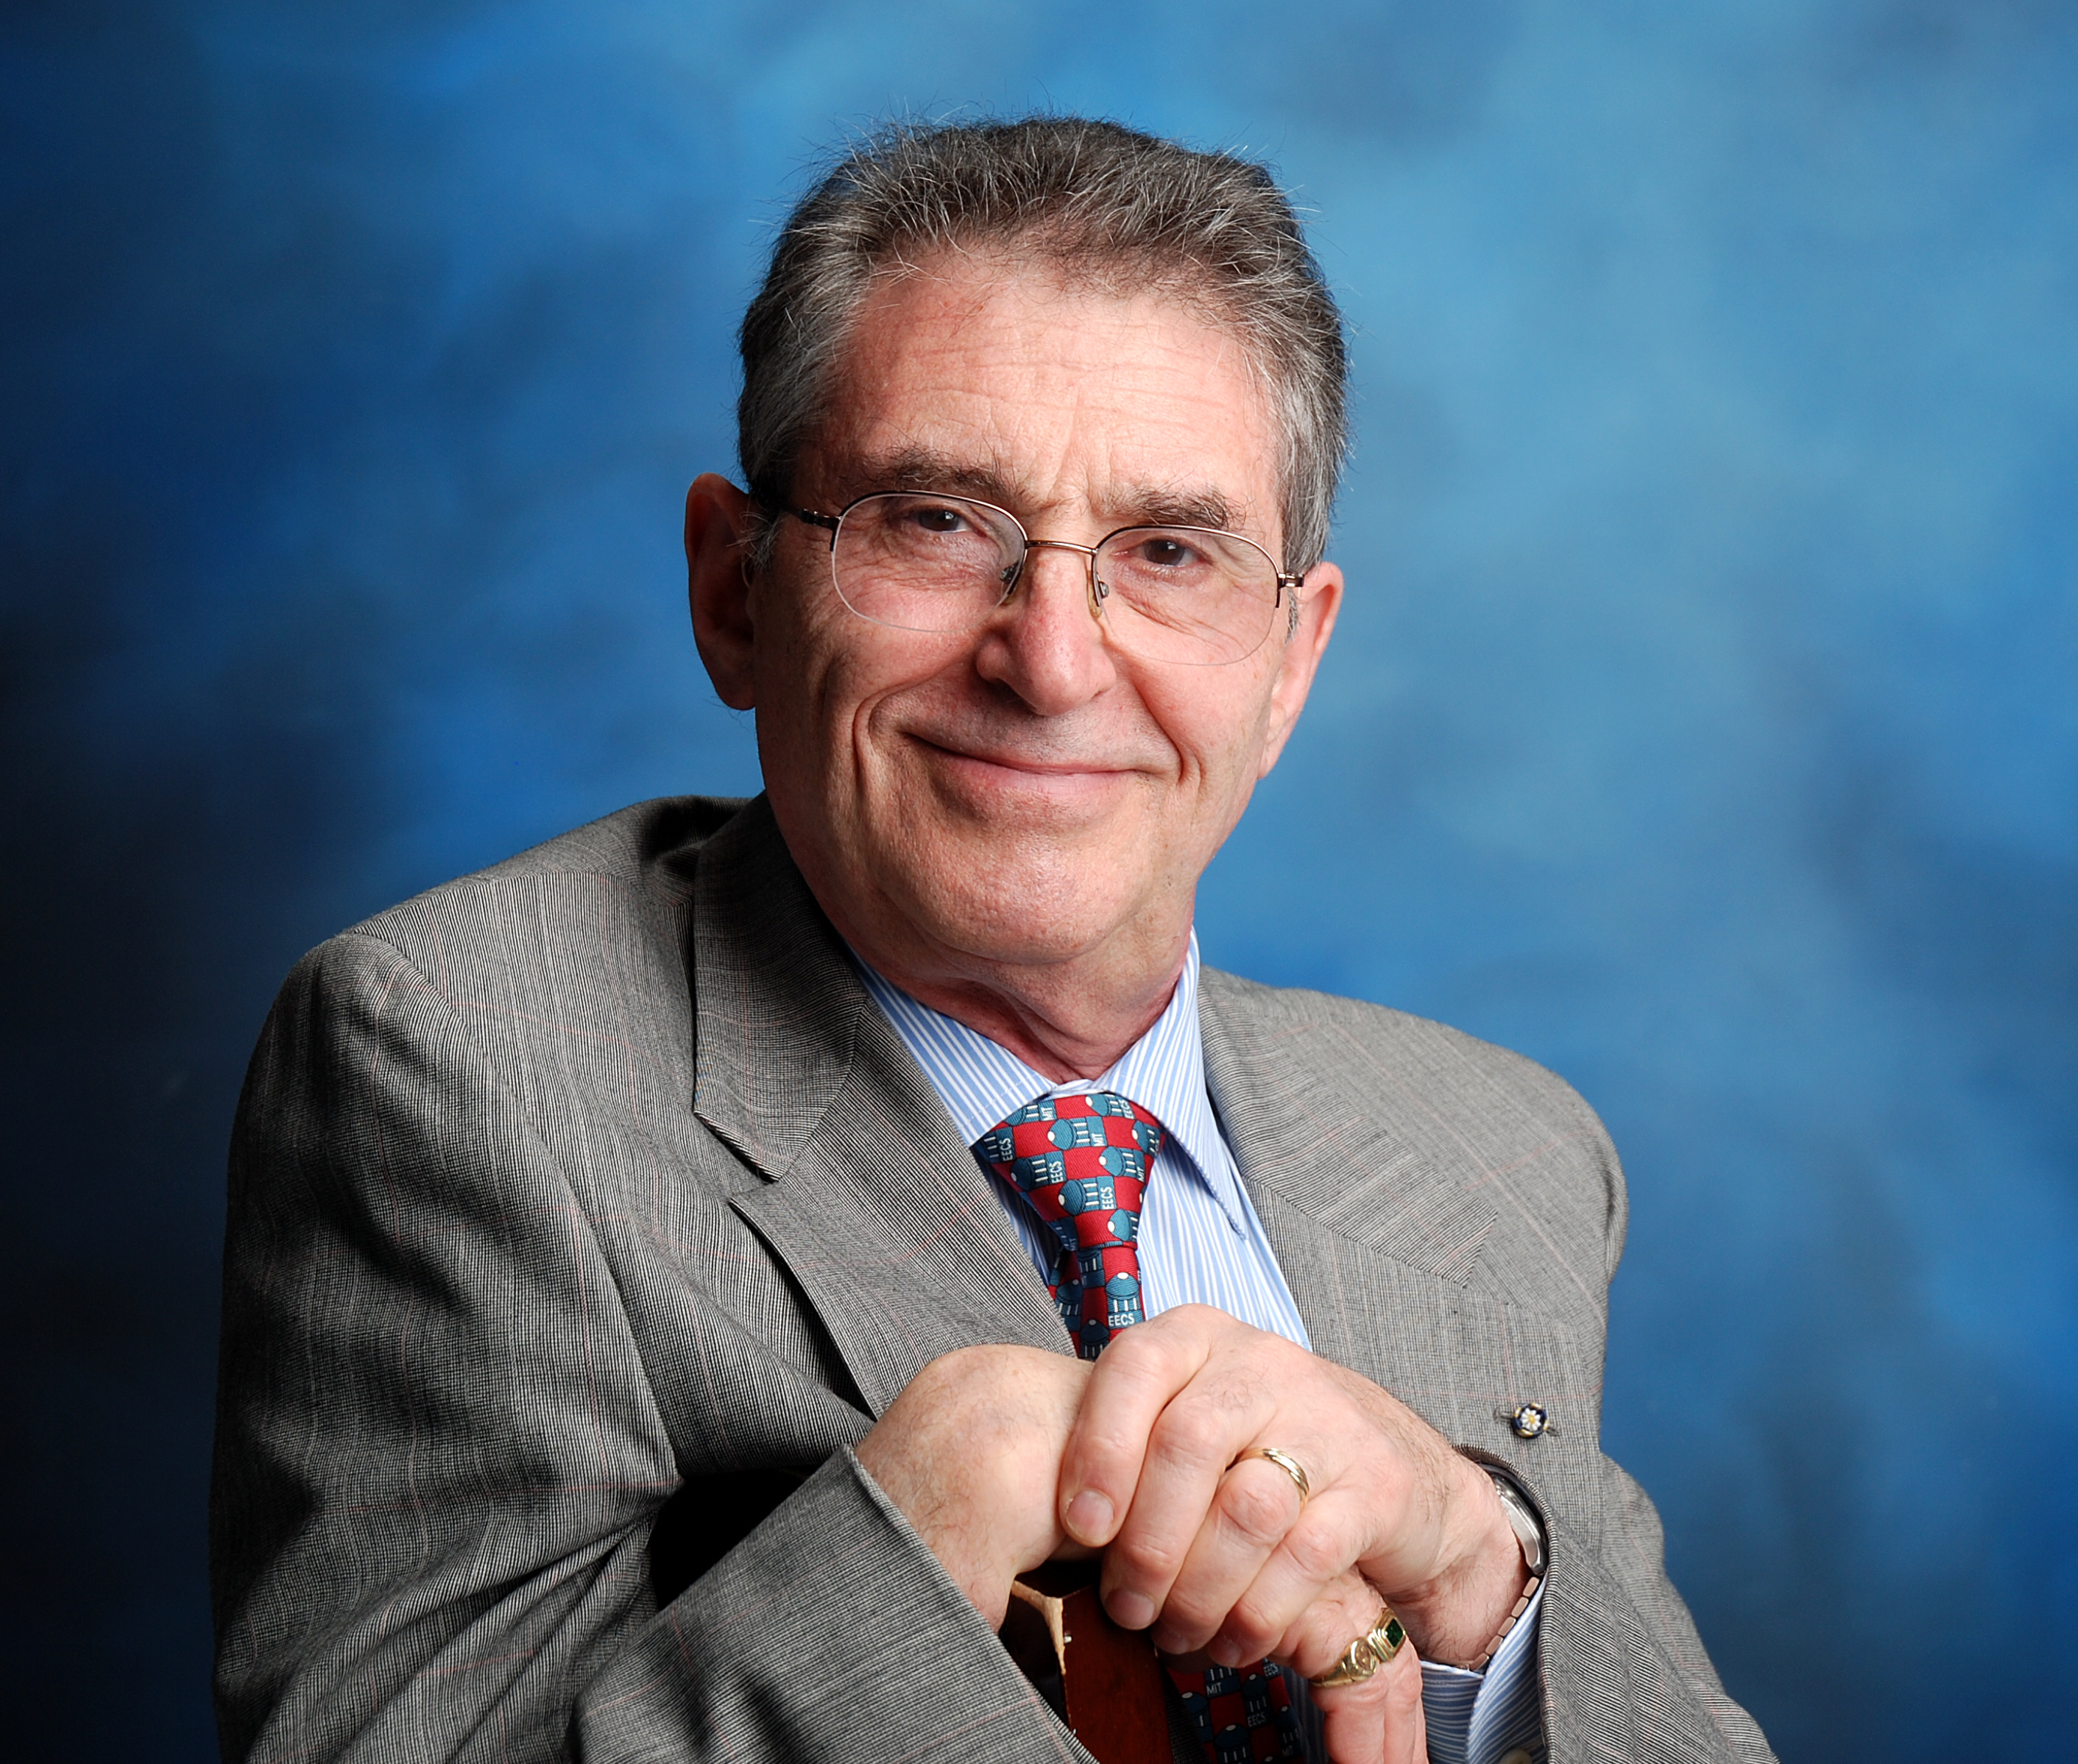
\includegraphics[height=2cm]{prologue/pix/MayerA_PortraitSimple152752.jpg}% 
  \quad %\vspace*{1ex}
  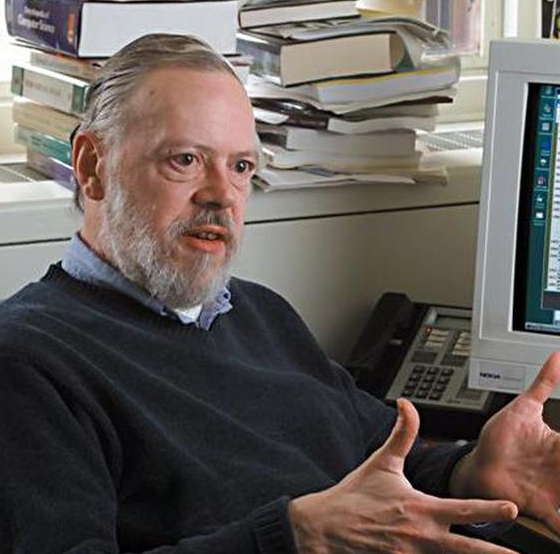
\includegraphics[height=2cm]{prologue/pix/ritchie.jpg}}% 
  \wrapcaption{\label{fig:mayer}\href{https://en.wikipedia.org/wiki/Albert_R._Meyer}{Albert Meyer b~1941} 与 \label{fig:ritchie}\href{https://en.wikipedia.org/wiki/Dennis_Ritchie}{Dennis Ritchie 1941--2011}}\index{Ritchie, D!picture}\index{Meyer, A!picture}
\end{wrapfigure}


%\margingraphic[l]{0.21\textwidth}{prologue/pix/ritchie.jpg}{\label{fig:ritchie}\href{https://en.wikipedia.org/wiki/Dennis_Ritchie}{Dennis Ritchie 1941--2011, inventor of C}}\index{Ritchie, D!picture}
Albert Meyer（阿尔伯特·迈耶）与 C 语言发明者 Dennis Ritchie（丹尼斯·里奇）研究了这一方向。我们将证明这个结论的一半：如果一个函数是原始递归的，那么我们可以只用有界循环来计算它。
具体做法是，在名为\citetext{\definend{LOOP 程序}}{%
  \protect\autocite{MeyerRitchie}}\index{LOOP program!language} 的语言中，为原始递归函数编写程序，
这种语言没有无界循环。
（其逆命题的证明超出了本书范围。）

% Picture from web page https://people.csail.mit.edu/meyer/; permission from A Meyer via email 2023-Feb-20 
%\margingraphic{0.21\textwidth}{prologue/pix/MayerA_PortraitSimple152752.jpg}{\label{fig:mayer}\href{https://en.wikipedia.org/wiki/Albert_R._Meyer}{Albert Meyer b~1941}}\index{Meyer, A!picture}
LOOP\index{LOOP program} 程序在一个带有寄存器的机器模型上执行，
寄存器 \codeinline{r0}、\codeinline{r1}、\ldots\ 可以存放自然数。
指令共有四种，我们使用 \codeinline{r0} 和 \codeinline{r1} 来描述它们：(i) \codeinline{r0 = 0}
将寄存器的内容设置为零，
(ii)~\codeinline{r0 = r0 + 1} 将寄存器的内容加一，
(iii)~\codeinline{r1 = r0} 将 \codeinline{r0} 的内容复制到 \codeinline{r1}，
而 \codeinline{r0} 保持不变，
以及 (iv)~\codeinline{loop r0 ... end}
重复执行一系列指令，
重复次数由该寄存器的值给定。
对于最后一种指令，`\codeinline{...}` 代表一个指令序列，它可以包含这四种语句中的任何一种，
包括嵌套的 \codeinline{loop}（该内层循环自身又可能包含嵌套的 \codeinline{loop}，依此类推）。

举个例子，下面的 LOOP 程序结束时，寄存器 \codeinline{r0} 中的值为 $4$，
而 \codeinline{r1} 中的值为~$2$（循环内的缩进只是为了视觉清晰）。
注意，除非在运行程序前预装载了机器，否则寄存器的初始值都是零。
\lstinputlisting{\prfiles machines/simple.loop}

非常重要的是：在循环内部改变循环寄存器的内容，
并不会改变机器执行该循环的次数。
因此，下面的代码并不是一个无限循环。
\begin{lstlisting}
loop r0 
  r0 = r0 + 1
  end  
\end{lstlisting}
相反，
当循环结束时，\codeinline{r0} 中的值将是循环开始时的两倍。

为了将 LOOP 程序解释为计算函数，我们需要对输入和输出作一些约定。
对于一个接收 $n$ 个输入的函数，我们会将这 $n$ 个输入预装载到机器的前 $n$ 个寄存器中。
类似地，对于一个有 $m$ 个输出的函数，我们取前 $m$ 个寄存器的最终值作为这 $m$ 个输出。

根据此约定，这个 LOOP 程序计算的是双输入、单输出的加法函数 $\plus(x,y)=x+y$。
\lstinputlisting{\prfiles machines/plus.loop}
本书的源代码包中附带一个 Racket 程序 \codeinline{loop.rkt}，它可以解释 LOOP 代码。
下面是运行该代码的一个调用示例。\footnote{%
  Racket 版本 8.2。}
\begin{lstlisting}
jim@millstone:src/scheme/prologue$ ./loop.rkt -f machines/plus.loop -p "3 2" -s
r0=3 r1=2
  --start loop of 2 repetitions--
  r0=4 r1=2
  r0=5 r1=2
  --end loop--
5
\end{lstlisting}  % $
程序的选项有：\codeinline{p} 将寄存器 \codeinline{r0} 和~\codeinline{r1} 预装载为 $3$ 和 $2$，
而 \codeinline{s} 则显示计算过程中每一步的寄存器状态。
默认情况下，模拟器返回第一个寄存器的值，此处为~$5$。

这个 LOOP 程序计算的是乘法函数 $\product(x,y)=x\cdot y$。
\lstinputlisting{\prfiles machines/product.loop}
它包含一个嵌套循环。
\begin{lstlisting}
jim@millstone:src/scheme/prologue$ ./loop.rkt -f machines/product.loop -p "3 2" -s
r0=3 r1=2
r0=3 r1=2 r2=2
r0=3 r1=3 r2=2
r0=0 r1=3 r2=2
  --start loop of 2 repetitions--
    --start loop of 3 repetitions--
    r0=1 r1=3 r2=2
    r0=2 r1=3 r2=2
    r0=3 r1=3 r2=2
    --end loop--
    --start loop of 3 repetitions--
    r0=4 r1=3 r2=2
    r0=5 r1=3 r2=2
    r0=6 r1=3 r2=2
    --end loop--
  --end loop--
6
\end{lstlisting}  % $

再看两个例子。
这个程序计算前驱函数 $\pred(x)$，
\lstinputlisting{\prfiles machines/pred.loop}
当 $x$ 不等于~$0$ 时，它等于 $x-1$；当 $x$ 等于~$0$ 时，它等于~$0$。
\begin{lstlisting}
jim@millstone:src/scheme/prologue$ ./loop.rkt -f machines/pred.loop -p "3" -s
r0=3
  --start loop of 3 repetitions--
  r0=3 r1=0 r2=0
  r0=3 r1=1 r2=0
  r0=3 r1=1 r2=1
  r0=3 r1=2 r2=1
  r0=3 r1=2 r2=2
  r0=3 r1=3 r2=2
  --end loop--
r0=2 r1=3 r2=2
2
\end{lstlisting}  % $
而这个程序利用前驱函数来计算截断减法 $x\dotminus y$，
\lstinputlisting{\prfiles machines/proper-sub.loop}
当 $y$ 不大于 $x$ 时，它等于 $x-y$；否则，结果为~$0$。
\begin{lstlisting}
jim@millstone:src/scheme/prologue$ ./loop.rkt -f machines/proper-sub.loop -p "3 2" -s
r0=3 r1=2
  --start loop of 2 repetitions--
  r0=3 r1=2 r3=0
    --start loop of 3 repetitions--
    r0=3 r1=2 r2=0 r3=0
    r0=3 r1=2 r2=0 r3=1
    r0=3 r1=2 r2=1 r3=1
    r0=3 r1=2 r2=1 r3=2
    r0=3 r1=2 r2=2 r3=2
    r0=3 r1=2 r2=2 r3=3
    --end loop--
  r0=2 r1=2 r2=2 r3=3
  r0=2 r1=2 r2=2 r3=0
    --start loop of 2 repetitions--
    r0=2 r1=2 r2=0 r3=0
    r0=2 r1=2 r2=0 r3=1
    r0=2 r1=2 r2=1 r3=1
    r0=2 r1=2 r2=1 r3=2
    --end loop--
  r0=1 r1=2 r2=1 r3=2
  --end loop--
1
\end{lstlisting}  % $

最后，这个例子展示了一个有多个输出的程序。
\lstinputlisting{\prfiles machines/rotate-shift-right.loop}
程序的 \codeinline{o} 选项让我们可以显示三个寄存器，而不是默认的一个，
\begin{lstlisting}
jim@millstone$ ./loop.rkt -f machines/rotate-shift-right.loop -p "1 2 3" -o 3
3 1 2
\end{lstlisting}  % $
（我们通过不使用 \codeinline{s} 选项避免了显示计算步骤）。

现在我们准备证明，对于每个原始递归函数，都存在一个计算它的 LOOP 程序。
策略是首先展示如何计算初始函数，然后展示如何实现函数复合与原始递归这两种组合运算。

零函数~$\zero(x)=0$ 可以用单行 LOOP 程序 \codeinline{r0 = 0} 来计算。
后继函数 $\successor(x)=x+1$ 可以用单行程序 \codeinline{r0 = r0 + 1} 来计算。
投影 $\projection_i(x_0,\ldots x_i,\ldots x_{n-1})=x_i$
可以用 \codeinline{r0 = r}$i$ 来计算。

两个函数的复合运算很容易。
设 $g(x_0,\ldots\, x_n)$ 和 $f(y_0,\ldots\, y_m)$
分别由 LOOP 程序 $P_g$ 和 $P_f$ 计算。
假设函数复合 $\composed{f}{g}$ 的参数对应是恰当的，即
$g$ 是一个 $m$ 输出函数，与 $f$ 的输入数量相匹配。
那么将这两个程序连接起来——也就是让 $P_g$ 的指令之后紧接着
$P_f$ 的指令——就得到了复合运算所需的 LOOP 程序，
因为它使用 $g$ 的输出作为输入来执行 $f$ 的计算。

一般化的复合运算从
\begin{equation*}
 f(x_0,\ldots\, x_n),
 \quad
 h_0(y_{0,0},\ldots\, y_{0,m_0}),
 \quad\ldots\quad
 h_n(y_{n,0},\ldots\, y_{n,m_n})
\end{equation*}
% $f(x_0,\ldots,x_n)$ 
% and $h_0(y_{0,0},\ldots,y_{0,m_0})$, \ldots  $h_n(y_{n,0},\ldots,y_{n,m_n})$
开始，并产生
$f(h_0(y_{0,0},\ldots y_{0,m_0}),\ldots h_n(y_{n,0},\ldots y_{n,m_n}))$。
这比两个函数的情况需要多一些思考。
问题在于，如果我们把输入 $y_{0,0}$, \ldots{} $y_{n,m_n}$ 装载到寄存器
\codeinline{r0}, \codeinline{r1}, \ldots{} 中，
然后立即开始计算 $h_0$，就会有覆盖后续函数（如 $h_1$）输入的危险。
例如，上面的 \codeinline{rotate-shift-right.loop} 就使用了一个额外的寄存器
\codeinline{r3}，它不在存储输入所用的寄存器之列。

因此我们必须把这些输入移开。
设 $P_f$, $P_{h_0}$, \ldots{} $P_{h_n}$
是计算这些函数的 LOOP 程序。
每个程序都使用有限数量的寄存器，
因此存在一个足够大的数~$j$，使得这些程序都不使用
寄存器~$j$。
根据定义，用来计算复合的程序~$P$
接收的输入序列从编号为~$0$ 的寄存器开始。
第一步是将这些输入复制到从寄存器~$j$ 开始的位置。
% (the final member will be copied to just before
% the register numbered $(m_0+1)+\cdots+(m_n+1)$).
接下来，将寄存器~$j$ 下方的寄存器清零，
将 $h_0$ 的参数向下复制到以 \codeinline{r0} 开头的位置，
然后运行程序 $P_{h_0}$。
当它执行完毕后，将其输出复制到编号为
$j+m_0+\cdots+ m_n+1$
的寄存器中。
对其他 $h_i$ 做类似处理。
最后，将这些输出向下复制到初始的寄存器，将剩余的寄存器清零，并运行 $P_f$。

另一个组合操作是原始递归。
\begin{equation*}
  f(x_0,\ldots\, x_{k-1},y)=
  \begin{cases}
    g(x_0,\ldots\, x_{k-1}) &\case{若 $y=0$}   \\
    h(f(x_0,\ldots\, x_{k-1},z),\,x_0,\ldots\, x_{k-1},\,z)
      &\case{若 $y=\successor(z)$}
  \end{cases}
\end{equation*}
假设我们有 LOOP 程序 $P_g$ 和~$P_h$。
所需的寄存器交换与复合运算的情况类似，所以我们就不再赘述了。
程序 $P_f$ 从运行 $P_g$ 开始。
然后它将一个新寄存器设为 $0$；称这个寄存器为~\codeinline{t}。
现在它进入一个基于寄存器~\codeinline{y} 的循环
（即，每次循环依次按 $y$, $y-1$ 等倒计数）。
循环体通过运行~$P_h$ 来计算
$f(x_0,\ldots\, x_{k-1},t+1)=h(f(x_0,\ldots x_{k-1},t),\,x_0,\ldots\, x_{k-1},t)$，
然后递增~\codeinline{t}。
至此论证完毕。

我们以关于 \codeinline{loop.rkt} 一个有趣方面的备注作为结尾，
\citetext{它是 LOOP 的解释器}{%
  改编自 \autocite{Schnieder}}。
它的工作原理是将上面使用的类 C 语法替换为类 LISP 的语法。
例如，解释器将左侧的字符串输入转换为右侧的字符串。


\begin{center}
  \begin{minipage}[t]{0.45\linewidth}
\begin{lstlisting}
r1 = r1 + 1
loop r1
  r0 = r0 + 1
  end
\end{lstlisting}
  \end{minipage}
  \qquad
  \begin{minipage}[t]{0.45\linewidth}
\begin{lstlisting}
((incr r1) (loop r1 (incr r0)))      
\end{lstlisting}
  \end{minipage}
\end{center}


这种转换的好处是括号能自动将每个 \codeinline{loop} 的开头与其
\codeinline{end} 匹配，
这样我们就不必在解释器中编写包含栈的代码来跟踪循环嵌套。
对于右侧的字符串，\codeinline{loop.rkt} 通过将其传入 \codeinline{eval} 命令来运行并计算出结果。

% ......................................
\begin{exercises}


\begin{exercise}
编写一个 LOOP 程序，输入两个数并交换它们，
使得 $x,y$ 变为 $y,x$。   
\begin{answer}\verified
代码如下。
\lstinputlisting{scheme/prologue/machines/swap-two.loop} 
这是一个示例调用。
\begin{lstlisting}
jim@millstone:src/scheme/prologue$ ./loop.rkt -f machines/swap-two.loop -p "1 2 3" -o 2
2 1
\end{lstlisting}
\end{answer} % $
\end{exercise}

\begin{exercise}
论证如果允许像 \codeinline{r0 = r0 + 2} 这样的语句，
或者像 \codeinline{r0 = 1} 这样的语句，LOOP 语言并不会变得更强大。    
\begin{answer}\verified
我们可以用连续两次递增来实现第一种的效果，
而第二种的效果可以通过先清零再递增来实现。  
\end{answer}
\end{exercise}

\begin{exercise}
程序 \codeinline{rotate-shift-right.loop} 输入 
三个数，输出三个数，
并将输入右移（第三个数最终进入第一个寄存器）。
编写一个三输入/三输出的程序，实现左循环移位。
同时编写复合这两个程序的程序。
它计算什么？
\begin{answer}\verified
左旋转代码是对右旋转代码的改编。
\lstinputlisting{scheme/prologue/machines/rotate-shift-left.loop} 
这是一个示例调用。
\begin{lstlisting}
jim@millstone:src/scheme/prologue$ ./loop.rkt -f machines/rotate-shift-left.loop -p "1 2 3" -o 3
2 3 1
\end{lstlisting}  % $
将两者组合起来得到如下程序。
\lstinputlisting{scheme/prologue/machines/concatenate-rotations.loop} 
这是一个示例调用。
\begin{lstlisting}
jim@millstone:src/scheme/prologue$ ./loop.rkt -f machines/concatenate-rotations.loop -p "1 2 3" -o 3
1 2 3
\end{lstlisting}  % $
\end{answer} 
\end{exercise}

\begin{exercise}
在 Ackermann 函数中，
在运算 $\plus(x,y)$ 和 $\product(x,y)$ 之后是 $\power(x,y)$。
为它写一个 LOOP 程序。
\begin{answer}\verified
下面是一个程序。
\lstinputlisting{scheme/prologue/machines/power.loop} 
这里是两个示例调用。
\begin{lstlisting}
jim@millstone:src/scheme/prologue$ ./loop.rkt -f machines/power.loop -p "3 2"
9
jim@millstone:src/scheme/prologue$ ./loop.rkt -f machines/power.loop -p "3 0"
1
\end{lstlisting}
\end{answer} % $
\end{exercise}

\begin{exercise}
如果你试图在 Racket 的循环内部修改循环变量，会发生什么？
例如，下面这两个程序的行为分别是什么？
\begin{center}
  \begin{minipage}{0.4\linewidth}
    \begin{lstlisting}
(for ([i (in-range 5)])
  (set! i 1)
  (displayln (~a "i=" i)))
\end{lstlisting}
  \end{minipage}
  \qquad
  \begin{minipage}{0.4\linewidth}
    \begin{lstlisting}
(for ([i (in-range 5)])
  (displayln (~a "i=" i))
  (set! i 1))
\end{lstlisting}
  \end{minipage}
\end{center}
\begin{answer}
第一个程序是这样的；请注意它运行了五次。
\begin{lstlisting}
 > (for ([i (in-range 5)])
    (set! i 1)
    (displayln (~a "i=" i)))
i=1
i=1
i=1
i=1
i=1    
\end{lstlisting}
第二个程序是这样的。
\begin{lstlisting}
> (for ([i (in-range 5)])
    (displayln (~a "i=" i))
    (set! i 1))
i=0
i=1
i=2
i=3
i=4     
\end{lstlisting}
\end{answer}
\end{exercise}

\end{exercises}
\index{LOOP program|)}

\renewcommand{\asydir}{background/asy/}


\begin{Filesave}{\answerbodyfilename}
  \def\asydir{background/asy/} % Graphics from correct directory for this chapter
\end{Filesave}

\chapteropen[这是哈勃深场图像。它来源于将哈勃望远镜指向天空最暗的部分——即背景深处——持续 11 天。它所覆盖的天空区域，大约相当于在 75 英尺外观看一枚一角硬币的宽度。图中的每一个斑点都是一个星系，其中有成千上万个——背景中内容丰富。致谢：Robert Williams 及哈勃深场团队（STScI）与 NASA。（另参见 \citetext{深场影片}{https://www.youtube.com/watch?v=yDiD8F9ItX0}。）]{background/pix/hubble.jpg}{背景}% https://www.nationalgeographic.com/science/phenomena/2015/04/24/when-hubble-stared-at-nothing-for-100-hours/


\begin{credit}
图片来源：Robert Williams 及哈勃深场团队（STScI）与 NASA。
\end{credit}

% See also https://i.imgur.com/Ym0Dke5.gifv

% Here we will develop the ideas surrounding the definition of
% mechanical computation.
% We will see several results that are a theme throughout the subject.

% The first chapter began by saying that we are more interested in what
% things can be computed than in the details of
% how they are computed.
我们希望理解那些有效的、机械可计算的函数集合，
也就是我们定义为可由 Turing 机计算的函数集合。
本章的主要结果（也是全书最重要的结果）是：
存在任何机器都无法计算的函数——存在没有机器能完成的工作。
我们将首先用计数论证来证明这一点，然后在本章后面给出具体的不可解问题。

% ========================================================
\section{无穷}\index{infinity|(}

我们将证明，函数 $\map{f}{\N}{\N}$ 的数量多于 Turing 机的数量，因此存在没有对应机器的函数。

\subsection{势}\index{cardinality|(}
\margingraphic{0.16\textwidth}{background/pix/galileo.jpg}{\label{fig:galileo}\href{http://en.wikipedia.org/wiki/Galileo_Galilei}{Galileo Galilei 1564--1642}}\index{Galilei, Galileo!picture}\index{Galileo|see {Galilei, Galileo}}%


\begin{credit}
图片来源：File:Galilee.jpg. (2018, September 27).
\textit{Wikimedia Commons, the free media repository}.
检索于 22:19, January 26, 2020，自
\protect\url{https://commons.wikimedia.org/w/index.php?title=File:Galilee.jpg&oldid=322065651}。
\end{credit}

函数集合和 Turing 机集合都是无限的。
我们将从 \citetext{两个悖论}{%
  Quine 称这些为真实悖论：它们起初可能显得荒谬，但我们将证明它们却是真的。
  \autocite{wiki:Paradoxes}}开始，
它们突显了在比较无限集大小时直觉所面临的挑战。
然后我们将给出解决这些谜题的数学工具，并将其应用于函数集合和 Turing 机集合。

第一个谜题是
\citetext{\definend{Galileo 悖论}}{%
  他并非发明者，但
  他在其著名的《关于两门新科学的对话和数学证明》中使其广为人知。}.\index{Galileo's Paradox}\index{paradox!Galileo's}
它比较了完全平方数集合与自然数集合的大小。
前者是后者的真子集，因此可能看起来在某种意义上更小。
然而，下图表明这两个集合可以逐元素地对应起来，
所以在这个意义上，平方数的个数与自然数的个数恰好一样多。
\ifbool{MakingPaperCopy}{%


\begin{fig}{自然数与平方数之间的对应 $n\leftrightarrow n^2$。}
  \includegraphics{\asydir galileo/galileo000}
  \end{fig}


}{%


\begin{animatedfigure}{自然数与平方数之间的对应 $n\leftrightarrow n^2$。}
  \animategraphics[poster=first]{3}{\asydir galileo/galileo}{000}{012}
  \end{animatedfigure}


}
第二个谜题是
\definend{Aristotle 悖论}.\index{Aristotle's Paradox}\index{paradox!Aristotle's}
下图左侧有两个圆。
如果让它们滚动一周，那么较小圆留下的轨迹较短。
但如果将小圆放在大圆内部一起滚动（就像火车轮那样），
那么它们似乎留下了等长的轨迹。

\begin{center}
  \begin{minipage}[b]{0.5\linewidth}
    \ifbool{MakingPaperCopy}{%
      \begin{fig}{半径不同的圆，其周长也不同。} \centering
        \includegraphics{\asydir aristotle/aristotle1050}
      \end{fig}
    }{%
      \begin{animatedfigure}{半径不同的圆，其周长也不同。} \centering
        \animategraphics[poster=last]{12}{\asydir aristotle/aristotle1}{000}{050}
      \end{animatedfigure}
    }
  \end{minipage}
  \hspace{1em}
  \begin{minipage}[b]{0.45\linewidth}
    \ifbool{MakingPaperCopy}{%
      \begin{fig}{嵌套的圆一起滚动。}\centering
        \includegraphics{\asydir aristotle/aristotle2050}
      \end{fig}
    }{%
      \begin{animatedfigure}{嵌套的圆一起滚动。}\centering
        \animategraphics[poster=last]{12}{\asydir aristotle/aristotle2}{000}{050}
      \end{animatedfigure}
    }
  \end{minipage}
% \hspace*{2em}\animategraphics{12}{\asydir aristotle/aristotle1}{000}{050}
% \hspace*{\fill}
% \animategraphics{12}{\asydir aristotle/aristotle2}{000}{050}\hspace*{2em}
\end{center}


与 Galileo 悖论类似，人们可能认为小圆上的点构成的集合在某种意义上是更小的。
但是，逐点地看，小圆上的点与大圆上的点是可以对应的。
正确的看法是，这两个点集拥有相同数量的元素。

下面的动画以两种方式展示了点的匹配。
左边将它们显示为嵌套的圆，内部的点与外部的点相对应。
第二个动画将其展开，使圆周变成了线段，这样对于上方的每一个点，在底部都有一个与之匹配的点。
\ifbool{MakingPaperCopy}{%


\begin{fig}{圆周上的对应点
    $x\cdot(2\pi r_0)\leftrightarrow x\cdot(2\pi r_1)$。%
    % with $x\in\leftclosed{0}{1}$.
    }\centering
    \includegraphics{\asydir aristotle/aristotle3015}
  \end{fig}


}{%


\begin{animatedfigure}{圆周上的对应点
    $x\cdot(2\pi r_0)\leftrightarrow x\cdot(2\pi r_1)$。%
    % with $x\in\leftclosed{0}{1}$.
    }\centering
    \animategraphics[poster=2]{3}{\asydir aristotle/aristotle3}{000}{025}
  \end{animatedfigure}


}

一个\index{correspondence}\index{function!correspondence}对应被定义为一个既是一一的又是满射的函数。
函数~$\map{f}{D}{C}$ 是\index{one-to-one function}\index{function!one-to-one}一一的，如果对 $x_0,x_1\in D$，由 $f(x_0)=f(x_1)$ 能推出 $x_0=x_1$。
它是\index{onto function}\index{function!onto}满射的，如果对任意~$y\in C$，都存在~$x\in D$ 使得 $y=f(x)$。
（附录~\ref{sec:Functions} 为相关复习。）
% The sketches below show two non-correspondences.
在下图中，左边的映射是一一的但不是满射，因为存在一个陪域元素没有定义域元素与之对应。
右边的映射是满射但不是一一的，因为两个输入映射到了同一个输出。

\begin{center}
  \includegraphics{\asydir maps/maps01.pdf}
  \hspace*{5em}
  \includegraphics{\asydir maps/maps00.pdf}
\end{center}

%<*lem:OneToOneOntoFiniteSets>


\begin{lemma} \label{lem:OneToOneOntoFiniteSets}
对于一个定义域有限的函数，其定义域中的元素个数大于或等于其值域中的元素个数。
如果该函数是一一的，那么其定义域与值域有相同数量的元素；而如果它不是一一的，那么其定义域有更多的元素。
因此，两个有限集拥有相同数量的元素，当且仅当它们能对应，也就是说，当且仅当存在从一个集合到另一个集合的函数，并且该函数是一个对应。
\end{lemma}


%</lem:OneToOneOntoFiniteSets>

\begin{proof}
\zcref{exer:OneToOneOntoFiniteSets}.
\end{proof}

%<*lem:EquinumerosityIsEquivalence>


\begin{lemma} \label{lem:EquinumerosityIsEquivalence}
两个集合之间的"存在从一个到另一个的对应"这一关系是一个等价关系。
\end{lemma}


%</lem:EquinumerosityIsEquivalence>

\begin{proof}
自反性（任何集合与自身相关）是显然的，因为集合通过恒等函数与自身对应。
对于对称性，假设 $S_0$ 与~$S_1$ 相关，即存在一个对应 $\map{f}{S_0}{S_1}$，回想其逆 $\map{f^{-1}}{S_1}{S_0}$ 存在并且是反方向的一个对应。
对于传递性，假设 $S_0$ 与~$S_1$ 相关且 $S_1$ 与~$S_2$ 相关，即存在对应 $\map{f}{S_0}{S_1}$ 和 $\map{g}{S_1}{S_2}$。
同时回想，复合 $\map{\composed{g}{f}}{S_0}{S_2}$ 是一个对应。
\end{proof}

我们现在为这个关系取个名字。
这将 \zcref{lem:OneToOneOntoFiniteSets} 中关于"大小相同"集合的观察，从有限集推广到了无限集。

%<*def:Cardinality>

\begin{definition} \label{def:Cardinality}
如果两个集合之间存在一一对应，则它们具有\citetext{\definend{同势}}{%
  数有两种本性。
  第一，把昴星团称为“七姐妹”时，我们是将其视为一个集合，而不带有任何次序。
  第二则相反，提及“七宗罪”时，显然其中一些罪孽比其他的更重。
  第一种指涉关乎数的基数性质，第二种则关乎其序数性质。
  对于有限数，二者紧密相连，如\protect\zcref{lem:OneToOneOntoFiniteSets}所述，
  但对于无限数，二者却不再一致。}\index{cardinality!definition}\index{set!cardinality}，
或称\definend{等势}\index{equinumerous sets}\index{set!equinumerous}，
记作$\sizeof{S_0}=\sizeof{S_1}$。
\end{definition}


%</def:Cardinality>

\begin{example} \label{ex:PerfectSquaresCountable}
Galileo 悖论\index{Galileo's Paradox}在于，平方数的集合
$S=\set{n^2\suchthat n\in\N}$
与 $\N$ 同势，记作 $\sizeof{S}=\sizeof{\N}$。
函数 $\map{f}{\N}{S}$ 由 $f(n)=n^2$ 给出，
它是一一的，因为如果
$f(x_0)=f(x_1)$ 那么 $x_0^2=x_1^2$，且由于它们非负，可得 $x_0=x_1$。
它是满射的，因为根据 $S$ 的定义，陪域中的任意元素 $y\in S$ 都是定义域 $\N$ 中某个 $n$ 的平方。
\end{example}

\begin{example} \label{ex:RealIntervalsCorrespond}
Aristotle 悖论\index{Aristotle's Paradox}在于，对于 $r_0, r_1\in\R^+\!$，
区间 $\leftclosed{0}{2\pi r_0}$ 与区间 $\leftclosed{0}{2\pi r_1}$ 同势。
映射 $g(x)=(2\pi r_1/2\pi r_0)\cdot x$
是一个一一对应；验证留作\zcref{exer:VerifyAsParadox}。
\end{example}

\begin{example}
集合 $S_0=\set{0,1,2,3}$ 和 $S_1=\set{10,11,12,13}$
同势，即 $\sizeof{S_0}=\sizeof{S_1}$。
从 $S_0$ 到 $S_1$ 的一个对应是 $x\mapsto x+10$。
\end{example}

\begin{example}
大于零的自然数集合，
$\N^+=\set{1,2,\ldots}$，与 $\N$ 同势。
一个对应是 $\map{f}{\N}{\N^+}$，由 $n\mapsto n+1$ 给出。
\end{example}

\margingraphic[l]{.2\textwidth}{background/pix/GeorgCantor.png}{\label{fig:cantor}\href{http://en.wikipedia.org/wiki/Georg_Cantor}{Georg Cantor1845--\-1918}}\index{Cantor, G!picture} % https://upload.wikimedia.org/wikipedia/commons/6/67/Georg_Cantor3.jpg
\citetext{以这种方式比较集合大小}{%
  还有其他数学上比较无限集大小的方法。
  一种是“渐近密度”，这超出了我们的范围。}
\citetext{是由 G~Cantor 在 1870 年代提出的}{%
  由于他的发现，Cantor 被一位杰出的数学家、他以前的教授 L~Kronecker
  斥为“青年的腐蚀者”。那还是在埃尔维斯之前。}。
正如上文的悖论所生动展示的，\zcref{def:Cardinality} 引入了一个深刻的思想。
我们应当确信，它抓住了我们说集合具有“相同个数”元素时想表达的含义。
支持这一点的论据之一是，它是\zcref{lem:OneToOneOntoFiniteSets}的自然推广。
论据之二是\zcref{lem:EquinumerosityIsEquivalence}，它将集合划分成类，使得在同一类中的所有集合都具有相同的势。
也就是说，它为“等势”中的“等”字提供了依据。
最重要的支持性论据是，正如 Turing 对其机器的定义一样，Cantor 的定义本身极具说服力。
G\"odel 注意到了这一点，他写道：
“无论应用于无限集的‘数’意味着什么，我们当然希望它具有这样的性质：如果保持对象本身不变，而以任何方式改变……例如改变它们的颜色或在空间中的分布……属于某个类的对象的数量都不会改变。
然而由此立即可得，如果两个集合的元素能够建立一一对应，它们就会有相同的[势]，
\citetext{这就是 Cantor 的定义}{\autocite{Godel64}}。”

%<*def:FiniteInfinite>


\begin{definition}
如果集合与某个 $n\in\N$ 的 $\set{0,1,\ldots\, n}$ 同势，或者它是空集，那么它是\definend{有限的}\index{finite set}\index{set!finite}。
否则它是\definend{无限的}\index{infinite set}\index{set!infinite}。
\end{definition}


%</def:FiniteInfinite>

对我们而言，
\citetext{最重要的无限集是自然数集$\N=\set{0,1,2,\ldots}$}{%
  它的存在由无穷公理保证，这是数学的标准公理之一，即 Zermelo-Frankel 公理。}。

%<*def:Countable>


\begin{definition}  \label{def:Countable}
一个与自然数集同势的集合是\definend{可数无限的}\index{countably infinite set}\index{set!countably infinite}。
一个有限或可数无限的集合是\definend{可数的}\index{countable set}\index{set!countable}。
如果一个集合是某个定义域为自然数的函数的值域，
那么我们说该函数\definend{枚举}\index{enumerate}\index{function!enumeration}该集合，
或\definend{是……的一个枚举}。\footnotemark[1]
\end{definition}

\footnotetext[1]{%
  “定义域为自然数的函数”这一说法似乎暗示该函数是全函数，但在 \zcref{sec:ComputablyEnumerableSets} 中，我们将把此概念应用于一些非全函数，即那些在某些自然数上没有定义的函数。
}
%</def:Countable>

“枚举”一词背后的思想是，函数 $\map{f}{\N}{S}$ 列出了它的值域：先是 $f(0)$，然后是 $f(1)$，依此类推。
（此列表可能有重复项，即 $f(n_0)=f(n_1)$ 但 $n_0\neq n_1$。）
我们通常对可计算的枚举感兴趣。

% As always, we are particularly interested in functions that are computable
% and all the examples below are computable.\footnote{%
%   To produce noncomputable correspondences we would need
%   material that we have not yet covered.}

\begin{example} \label{ex:MultiplesOfThreeCountable}
由 3 的倍数组成的集合 $3\N=\set{3k\suchthat k\in\N}$ 是可数的。
自然的映射 $\map{g}{\N}{3\N}$ 是 $g(n)=3n$。
\end{example}

\begin{example} \label{ex:NWithGapsCountable}
集合 $\N-\set{2,5}=\set{0,1,3,4,6,7,\ldots}$ 是可数的。
下面的函数填补了空缺，同时给出了形式化定义和表格说明。
\begin{equation*}
  f(n)=\begin{cases}
         n    &\case{if $n<2$}  \\
         n+1  &\case{if $n\in\set{2,3}$} \\
         n+2  &\case{if $n\geq 4$}
       \end{cases}
  \quad
  \begin{array}{r|ccccccc@{\hspace{6pt}}c}
    n
      &0 &1 &2 &3 &4 &5 &6 &\ldots \\ \cline{2-9}
    f(n)
      &0
      &1
      &3
      &4
      &6
      &7
      &8
      &\ldots
  \end{array}
  \qquad
\end{equation*}
这个函数显然既是一一的又是满射的。
\end{example}

%<*ex:SetOfPrimesCountable>


\begin{example} \label{ex:PrimesCountable}
质数集合~$P$ 是可数的。
存在一个函数~$\map{p}{\N}{P}$，其中 $p(n)$ 是第 $n$ 个质数，即 $p(0)=2$，$p(1)=3$，依此类推。
\end{example}


%</ex:SetOfPrimesCountable>

\begin{example}  \label{ex:StringsCountable}
取定符号集 $\Sigma=\set{\str{a},\ldots\,\str{z}}$。
考虑由这些符号构成的串的集合，例如 \str{az} 和~\str{abba}。
所有此类串的集合 $\kleenestar{\Sigma}\!$,\index{Kleene star} 是可数的。
下表展示了一种对应，即把串按
\citetext{\definend{字典序（lexicographic order）}}{%
  有时也称为词典序或字母序。}\index{lexicographic order}排列，
其中较短的串排在较长的串之前，而长度相同的串则按字母顺序排列。
（第一项是空串，
$\emptystring=\text{‘$\mskip 2mu$’}$。）\index{string!empty}\index{empty string@empty string, $\emptystring$}
\begin{center}
  \begin{tabular}{r|ccc@{\hspace{6pt}}c@{\hspace{6pt}}ccc@{\hspace{6pt}}c}
    自然数 $n\in\N$  &$0$    &$1$   &$2$ &$\ldots$  &$26$  &$27$ &$28$ &$\ldots$   \\
    \cline{2-9}
    符号串 $f(n)\in\kleenestar{\Sigma}$  &$\emptystring$  &\str{a} &\str{b} &$\ldots$
    &\str{z} &\str{aa} &\str{ab}  &$\ldots$
  \end{tabular}
\end{center}
\end{example}

%<*ex:SetOfIntegersCountable>


\begin{example} \label{ex:ZIsCountable}
整数集 $\Z=\set{\ldots,-2,-1,0,1,2,\ldots}$ 是可数的。
一种自然的对应是在正数和负数之间交替。
\begin{equation*}
  \begin{array}{r|*{7}{c}@{\hspace{6pt}}c}
    n\in\N  &0    &1   &2 &3  &4  &5  &6 &\ldots
   \\ \cline{2-9}
    f(n)\in\Z  &0  &+1 &-1 &+2  &-2 &+3 &-3 &\ldots
  \end{array}
\end{equation*}
\end{example}


%</ex:SetOfIntegersCountable>

\zcref{ex:ZIsCountable} 又回到了关于无限的悖论。
我们可能会天真地以为，正数和负数合起来，会让 $\Z$ 在某种意义上是 $\N$ 的两倍大。
然而这正是 Galileo 悖论：\index{Galileo's Paradox}
衡量一个集合有多少元素的正确方法，不是看它包含或被包含，而是看它的势。

最后，我们提一下另一个悖论，
\ifbool{MakingPaperCopy}{%
  由 Zeno 提出。
}{%
  \citetext{由 Zeno 提出}{%
    Zeno 提出了一些与运动相关的悖论。
    参见 \autocite{wiki:Zeno}
    \autocite{sep:Zeno},
    \autocite{Bragg}，
    以及 \url{http://www.smbc-comics.com/comic/zeno}
    和下面这幅 \texttt{xkcd} 漫画。
    \protect

\begin{center} \protect\small
      \protect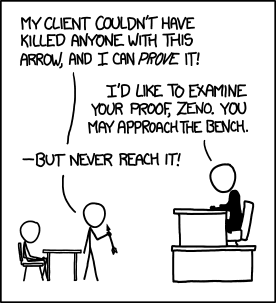
\includegraphics[width=0.2\textwidth]{background/pix/xkcdzeno.png}
    \\
    \protect\label{fig:xkcdzeno}\protect\href{https://xkcd.com/1153/}{由 \protect\url{xkcd.com} 提供}
    \protect\end{center}

}}\index{Zeno's Paradox}\index{paradox!Zeno's}（约公元前450年）。
他设想出一只慢吞吞的乌龟向敏捷的阿基里斯挑战赛跑，
只要求一点领先优势。
阿基里斯笑了，但乌龟说，等阿基里斯
跑到起跑领先位置~$x_0$ 时，乌龟早就已经前进到了某个点~$x_1$。
等跑到~$x_1$，阿基里斯会发现乌龟又跑到了~$x_2$。
对于任意的 $x_i$，
阿基里斯都会落在后面，因此乌龟推论道，阿基里斯永远不可能领先。
这个论证的核心在于，虽然\citetext{距离 $x_{i+1}-x_i$ 趋近于零，
  但由于区间 $\open{0}{\infty}$ 左端的开放性，
  永远有路要走}{%
  一个与此类似、利用了数的无界性的现代悖论是 Thomson 灯悖论：~a
  一个人打开房间的灯，一分钟后关掉，
  半分钟后再打开，四分之一分钟后再关掉，如此等等。
  两分钟后，灯是亮着还是关着？
  这个悖论由 J F~Thomson（汤姆森）于1954年提出，旨在
  分析超任务的可能性，即完成无限多个任务。J F~Thomson 的结论是这会产生矛盾：
  “灯不可能亮着，因为我从来没有只开灯而不立刻关掉它。
  灯也不可能关着，因为我一开始确实开了灯，并且
  此后我也从来没有只关灯而不立刻打开它。
  但灯要么亮着，要么关着”\autocite{Thomson}。
  另见关于
  Littlewood 悖论的讨论 \autocite{wiki:LittlewoodParadox}。}。


\begin{fig}{埃利亚的芝诺向青年们展示通往真理与谬误之门，% (\textit{Veritas et Falsitas})
  通过先走到门的一半距离，再走剩下的一半，如此等等。
  % Bartolomeo Carducci (1560-1608) or Pellegrino Tibaldi (1527–1596).}
  （作者为 B~Carducci（卡杜奇）（1560--1608）或 P~Tibaldi（蒂巴尔迪）（1527--1596）。）}
  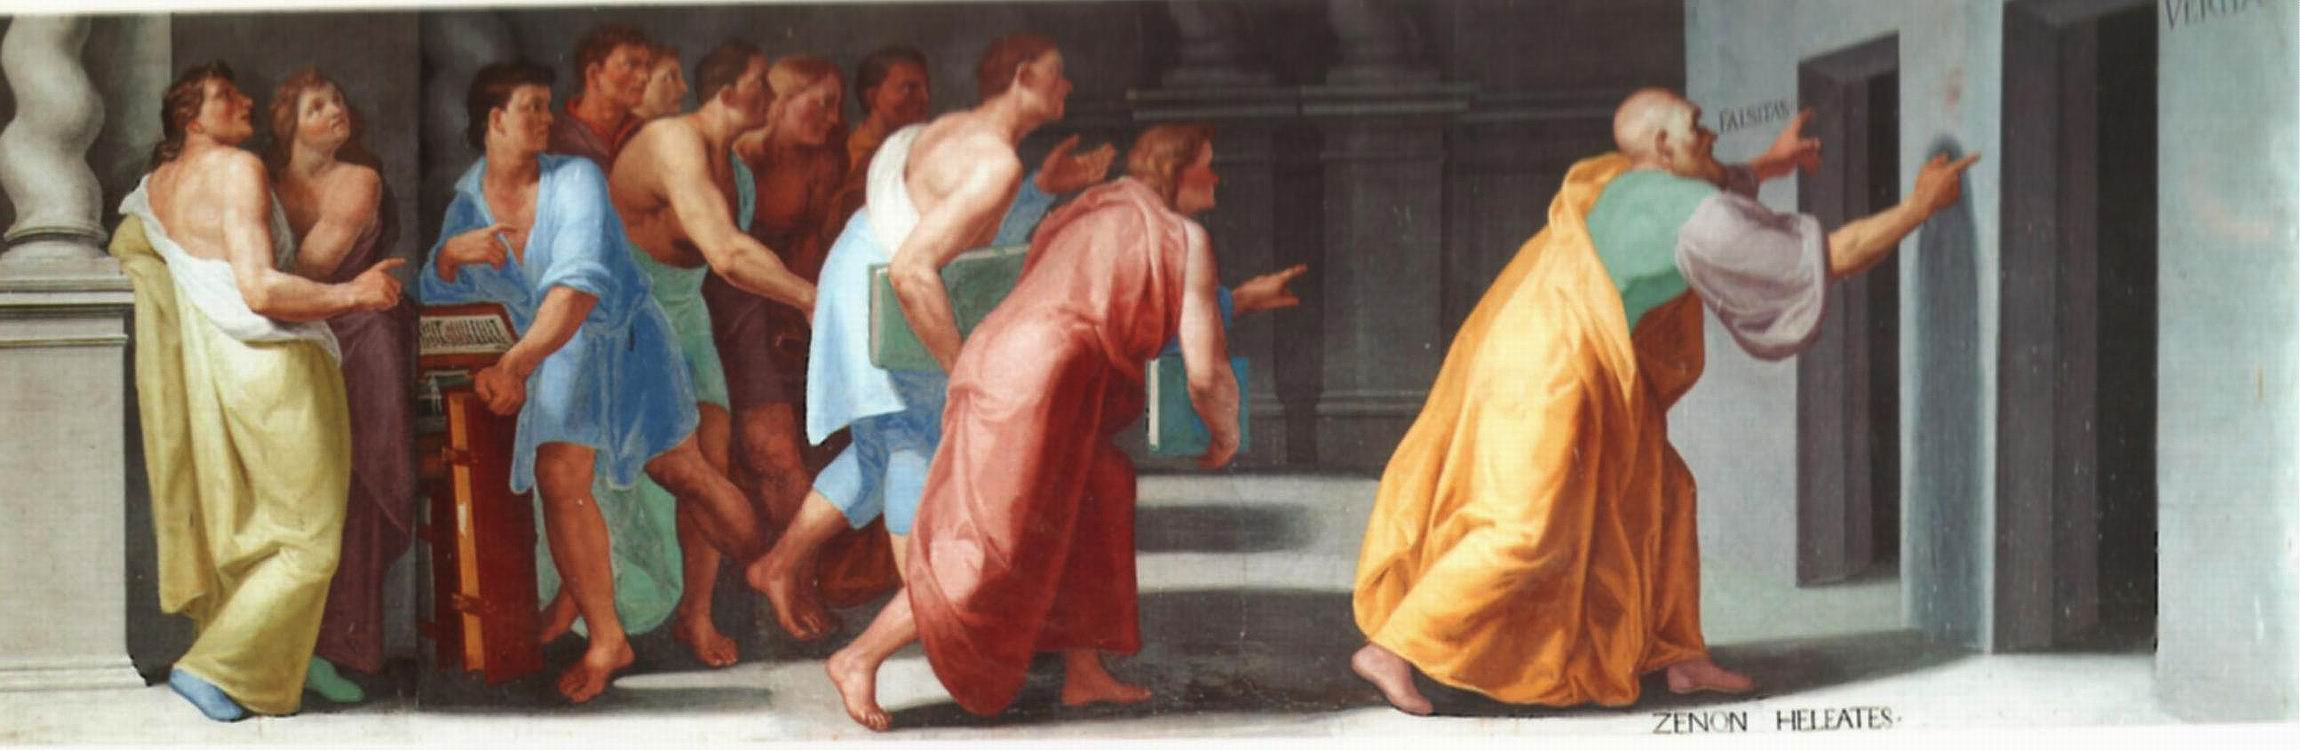
\includegraphics[width=0.8\textwidth]{background/pix/zeno.jpg}
  % PD: https://commons.wikimedia.org/wiki/File:Zeno_of_Elea_Tibaldi_or_Carducci_Escorial.jpg
\end{fig}


\noindent
这个悖论与本小节内容之间的联系，
以及本书后面给出的许多论证，
在于我们常常利用无界性。
不同之处在于，这里以及后面我们关注的是
自然数的无界性，即
$\N$ 在无穷远处的开放性。

\begin{exercises}
\recommended


\begin{exercise}
验证 \zcref{ex:MultiplesOfThreeCountable}，即由 $\map{g}{\N}{\set{3k\suchthat k\in\N}}$ $n\mapsto 3n$ 给出的函数
既是一一的又是满射的。
\begin{answer} \verified
为证明该映射是一一的，我们将证明 $g(n)=g(\hat{n})$ 仅当 $n=\hat{n}$ 时成立。
因此设 $g(n)=g(\hat{n})$，得 $3n=3\hat{n}$。
两边除以三得 $n=\hat{n}$。

为证明该映射是满射的，我们将证明陪域中每个成员
$y\in\set{3k\suchthat k\in\N}$ 都是定义域中某个成员的像。
因为 $y$ 是三的倍数，$y/3$ 是一个自然数。
由于 $y=g(y/3)$，可知 $y$ 确实是定义域中某个成员的像。
\end{answer}
\end{exercise}

\begin{exercise}
一位朋友说：“完全平方数和完全立方数的元素个数相同，因为这两个集合都
既是一一的又是满射的。”
这说法不对；纠正他们。
\begin{answer}  \verified
这是一个类型错误。
一一的或满射的不是集合本身；而是集合之间的对应关系 $f$。
对于 $D=\set{n^2\suchthat n\in\N}$ 和
$C=\set{n^3\suchthat n\in\N}$，自然的这种对应关系
$\map{f}{D}{C}$ 是 $f(n)= n^{3/2}$。
\end{answer}
\end{exercise}

\begin{exercise}
令 $\map{f,g}{\Z}{\Z}$ $f(x) = 2x$ 且 $g(x) = 2x-1$。
对以下各项给出证明或反例。
\begin{exparts*}
\item $f$ 是一一的吗？是满射的吗？
\item $g$ 是一一的吗？是满射的吗？
\item $f$ 和 $g$ 互为逆函数吗？
\end{exparts*}
\begin{answer}  \verified
\begin{exparts}
\item  由 $f(x) = 2x$ 给出的函数 $\map{f}{\Z}{\Z}$ 是一一的，但不是满射的。
  验证它为一一是常规做法：假设对于 $x,\hat{x}\in\Z$ 有 $f(x)=f(\hat{x})$，
  于是 $2x=2\hat{x}$，然后约去 $2$ 得到 $x=\hat{x}$。
  要证明它不是满射的，只需指出一个陪域元素 $y\in\Z$，
  它不是任何定义域元素的像。
  一个这样的例子是 $y=1$，因为每个定义域元素的像都是偶数。
\item  由 $g(x) = 2x-1$ 给出的函数 $\map{g}{\Z}{\Z}$ 也是一一的，但不是满射的。
  一一性的论证与上一项类似：假设对于 $x,\hat{x}\in\Z$ 有 $g(x)=g(\hat{x})$，
  于是 $2x-1=2\hat{x}-1$。
  两边加 $1$ 然后约去 $2$，得到 $x=\hat{x}$。
  这个函数不是满射的，因为陪域元素 $y=2$ 不是任何定义域元素的像，
  因为 $y=2$ 是偶数，而对任何输入整数 $x$，数 $2x-1$ 都是奇数。
\item  它们不互为逆函数。
  例如，$\composed{f}{g}\,(1)=f(g(1))=f(1)=2$。
\end{exparts}
\end{answer}
\end{exercise}

\recommended


\begin{exercise}  % credit: http://www.oxfordmathcenter.com/drupal7/node/205
判断以下每个函数是一一的、满射的、两者都是还是两者都不是。
不能只回答“是”或“否”，必须说明理由。
\begin{exparts}
\item 由 $f(n)=n+1$ 给出的函数 $\map{f}{\N}{\N}$
\item 由 $f(n)=n+1$ 给出的函数 $\map{f}{\Z}{\Z}$
\item 由 $f(n)=2n$ 给出的函数 $\map{f}{\N}{\N}$
\item 由 $f(n)=2n$ 给出的函数 $\map{f}{\Z}{\Z}$
% \item $\map{f}{\N}{\N}$ given by $f(n)=2n+1$
% \item $\map{f}{\Z}{\Z}$ given by $f(n)=2n+1$
% \item $\map{f}{\Z}{\N}$ given by $f(n)=|n|/2$
\item 由 $f(n)=\sizeof{n}$ 给出的函数 $\map{f}{\Z}{\N}$
\end{exparts}
\begin{answer} \verified
\begin{exparts}
\item 由 $f(n)=n+1$ 给出的函数 $\map{f}{\N}{\N}$ 是一一的但不是满射的。
  验证一一性：假定 $n_0,n_1\in\N$ 满足 $f(n_0)=f(n_1)$，
  从而 $n_0+1=n_1+1$，然后两边减去 $1$ 得到 $n_0=n_1$。
  它不是满射的，因为陪域元素 $0\in\N$ 不是任何定义域元素的像。
\item 由 $f(n)=n+1$ 给出的映射 $\map{f}{\Z}{\Z}$ 是一个对应——它既是一一的又是满射的。
  一一性验证：假定 $f(n_0)=f(n_1)$，
  从而 $n_0+1=n_1+1$，减去 $1$ 得到 $n_0=n_1$。
  满射性验证：固定某个陪域元素 $y\in\Z$，
  注意定义域元素 $x=y-1$ 满足 $f(x)=y$。
\item 由 $f(n)=2n$ 给出的函数 $\map{f}{\N}{\N}$ 是一一的但不是满射的。
  对于一一性，假定 $n_0,n_1\in\N$ 满足 $f(n_0)=f(n_1)$。
  于是 $2n_0=2n_1$，消去 $2$ 得到 $n_0=n_1$。
  它不是满射的，因为陪域元素 $y=1$ 不是任何定义域元素的像，因为所有的像都是偶数。
\item 由 $f(n)=2n$ 给出的函数 $\map{f}{\Z}{\Z}$ 是一一的但不是满射的。
  一一性验证与上一项类似：假定对于某些 $n_0,n_1\in\Z$ 有 $f(n_0)=f(n_1)$，
  则 $2n_0=2n_1$，消去 $2$ 得到 $n_0=n_1$。
  同样如上一项，此映射不是满射的，
  因为陪域元素 $y=1$ 不在函数的值域内，因为所有值域元素都是偶数。
\item 由 $f(n)=\sizeof{n}$ 给出的函数 $\map{f}{\Z}{\N}$ 不是一一的，但是满射的。
  它不是一一的，因为两个定义域元素 $n_0=-1$ 和 $n_1=1$ 映射到相同的输出：$f(n_0)=2=f(n_1)$。
  为证明 $f$ 是满射映射，考虑陪域元素 $y\in\N$，
  并注意到若取定义域元素 $x\in\Z$ 使得 $x=y$，那么有 $f(x)=y$。
\end{exparts}
\end{answer}
\end{exercise}

\begin{exercise}
判断以下每一个是否是对应（你必须加以验证）：
\begin{exparts*}
\item 由 $f(q)=q+3$ 给出的 $\map{f}{\Q}{\Q}$
\item 由 $f(n)=n+3$ 给出的 $\map{f}{\Z}{\Q}$
\item 由 $f(a/b)=\sizeof{a\cdot b}$ 给出的 $\map{f}{\Q}{\N}$
% \hint~this could be though of as a trick question.
\end{exparts*}
\begin{answer} \verified
\begin{exparts}
\item 这个函数是一个对应。
  要验证它是一一的，假定 $f(q_0)=f(q_1)$，
  其中 $q_0,q_1\in\Q$，
  从而 $q_0+3=q_1+3$，两边减去 $3$ 得到 $q_0=q_1$。
  对于满射性，考虑陪域元素 $y\in\Q$，
  注意由 $q=y-3$ 给出的定义域元素 $q\in\Q$ 满足 $f(q)=y$。
\item 这个函数不是一个对应。
  它不是满射的，因为陪域元素 $1/2 \in\Q$ 不是任何一个定义域元素 $z\in\Z$ 的像，
  因为每个这样的像 $f(z)=z+3$ 都是整数。
  （这个函数是一一的：假定 $f(z_0)=f(z_1)$，
  从而 $z_0+3=z_1+3$，两边减去 $3$ 得到 $z_0=z_1$。
  但由于它不是满射的，所以它不是对应。）
\item 这不是一个对应。
  它甚至不是一个函数，因为它不是良定义的——
  两个有理数 $q_0=1/2$ 和 $q_1=2/4$ 相等，即 $q_0=q_1$，
  但它们对应的 $\sizeof{a\cdot b}$ 值不同，
  因为 $\sizeof{1\cdot 2}=2$ 而 $\sizeof{2\cdot 4}=8$。
\end{exparts}
\end{answer}
\end{exercise}

\begin{exercise}
判断以下每个集合是有限的还是无限的，并论证你的答案。
\begin{exparts*}
\item $\set{1,2,3}$
\item $\set{0,1,4,9,16,\ldots}$
\item 素数集合
\item 方程 $x^5-5x^4+3x^2+7$ 的实根集合
\end{exparts*}
\begin{answer}  \verified
\begin{exparts}
\item 这个集合是有限的。
  它与 $I=\set{0,1,2}$ 有相同的势，
  由 $f(x)=x+1$ 给出的函数 $\map{f}{I}{\set{1,2,3}}$ 见证，通过观察可知该映射是一一的且满射的。
\item 由完全平方数组成的集合 $S=\set{0,1,4,9,16,\ldots}$ 是无限的。
  不存在 $I=\set{0,1,\ldots\, n-1}$ 和 $S$ 之间的对应，因为不存在满射函数——对于
  任何函数 $\map{f}{I}{S}$，集合 $\set{f(0),f(1),\ldots\, f(n-1)}$ 不可能等于 $S$，
  因为前者有一个最大元素，而 $S$ 没有最大元素。
\item 素数集合是无限的。
  上一项的论证同样适用。
\item 根据算术基本定理，一个五次多项式至多有五个实数根。
  因此这个集合的势至多为五，所以是有限的。
\end{exparts}
\end{answer}
\end{exercise}

% \begin{exercise}
% Prove that
% the set $\N-\set{0}=\set{1,2,\ldots}$ is countable, using as a correspondence
% the function $\map{f}{\N}{\N-\set{0}}$ given by
% $f(n)=n+1$.
% \begin{answer}
% The function $f$ is one-to-one because if $f(n_0)=f(n_1)$ then
% $n_0+1=n_1+1$ and so~$n_0=n_1$.
% It is onto because if $y$ is an element of the
% codomain~$\N-\set{0}=\set{1,2,\ldots}$ then $y$ is the image of $y-1$,
% that is, $y=f(y-1)$,
% and clearly $y-1$ is an element of the domain~$\N$.
% \end{answer}
% \end{exercise}

\begin{exercise}
通过构造从一个集合到另一个集合的一一的且满射的函数，来证明下列每对集合具有相同的势。
你必须验证该函数是一个对应。
\begin{exparts*}
\item $\set{0,1,2}$, $\set{3,4,5}$
\item $\Z$, $\set{i^3\suchthat i\in\Z}$
\end{exparts*}
\begin{answer} \verified
\begin{exparts}
\item 映射 $\map{f}{\set{0,1,2}}{\set{3,4,5}}$ 由 $f(0)=3$, $f(1)=4$, $f(2)=5$ 给出，即 $f(x)=x+3$，是一个对应。
  经检查，陪域中的每个元素都与定义域中唯一的一个元素相关联。
\item 函数 $f(x)=x^3$ 是这些集合之间的一个对应。
  对于每个完全立方数，都有且仅有一个与之关联的整数立方根。
\end{exparts}
\end{answer}
\end{exercise}

\recommended


\begin{exercise}
通过构造一个对应（你必须验证该函数是一个对应），来证明下列每对集合具有相同的势：
\begin{exparts*}
\item $\set{0,1,3,7}$ 和 $\set{\pi,\pi+1,\pi+2,\pi+3}$
\item 偶自然数与完全平方数
\item 实数区间 $\open{1}{4}$ 与 $\open{-1}{1}$。
\end{exparts*}
\begin{answer} \verified
\begin{exparts}
\item 函数 $f$ 由 $0\mapsto\pi$, $1\mapsto\pi+1$, $3\mapsto\pi+2$, $7\mapsto\pi+3$ 给出，经检查可知它既是一一的又是满射的。
\item 令 $E=\set{2n\suchthat n\in\N}$ 且 $S=\set{n^2\suchthat n\in\N}$。
  考虑由 $f(x)=(x/2)^2$ 给出的映射 $\map{f}{E}{S}$。
  为证明 $f$ 是一一的，假设 $f(x_0)=f(x_1)$。
  那么 $(x_0/2)^2=(x_1/2)^2$，并且由于这些是自然数，它们的平方根相等，即 $x_0/2=x_1/2$。
  因此 $x_0=x_1$，该映射是一一的。

  为证明满射性，任取 $y\in S$。
  因为 $y$ 是一个完全平方数，所以存在自然数 $n\in\N$ 使得 $y=n^2$。
  令 $x=2n$。
  显然 $x$ 是偶数，且 $f(x)=y$。
\item 第二个区间的宽度是第一个的 $2/3$，因此考虑函数 $f(x)=(2/3)\cdot x-(5/3)$。
  它是一一的，因为 $f(x_0)=f(x_1)$ 意味着 $(2/3)\cdot x_0-(5/3)=(2/3)\cdot x_1-(5/3)$，通过简单的代数运算可得 $x_0=x_1$。
  要证明 $f$ 是满射的，固定 $y\in\open{-1}{1}$。
  令 $x=(y+(5/3))\,/\,(2/3)$（这来自于从方程 $y=(2/3)x-(5/3)$ 解出 $x$）。
  当 $y$ 是陪域 $\open{-1}{1}$ 中的一个元素时，这个 $x$ 便是定义域 $\open{1}{4}$ 中的一个元素，并且进一步的代数运算表明 $f(x)=y$。
\end{exparts}
\end{answer}
\end{exercise}

\recommended


\begin{exercise}
验证函数 $f(x)=1/x$ 是 $\R$ 的子集 $\open{0}{1}$ 与~$\open{1}{\infty}$ 之间的一个对应。
\begin{answer} \verified
题目的表述在哪个集合是定义域、哪个是陪域方面有些含糊。
我们将证明由 $f(x)=1/x$ 给出的 $\map{f}{\open{0}{1}}{\open{1}{\infty}}$ 既是一一的又是满射的。

为证一一性，假设 $f(x_0)=f(x_1)$，其中 $x_0,x_1\in\open{0}{1}$。
那么 $1/x_0=1/x_1$，交叉相乘可得 $x_1=x_0$。
为证满射性，设 $y\in\open{1}{\infty}$，并注意到若取 $x=1/y$，则 $f(x)=y$ 且也有 $x\in\open{0}{1}$。
\end{answer}
\end{exercise}

\begin{exercise}
给出集合 $\set{1,2,3,4,\ldots}$ 与
$\set{7,10,13,16\ldots}$ 之间的对应的公式。
\begin{answer}\verified
将这两个集合记为 $D=\set{1,2,3,4,\ldots}$ 和
$C=\set{7,10,13,16\ldots}$。
我们将证明由公式 $f(x)=3(x-1)+7$ 所描述的映射 $\map{f}{D}{C}$ 是这两个集合之间的一个对应。
该函数是一一的，因为由 $f(x_0)=f(x_1)$ 可推出
$3(x_0-1)+7=3(x_1-1)+7$，然后减去 $7$，除以 $3$，再加 $1$ 便得到 $x_0=x_1$。
它是满射的，因为如果 $y$ 是陪域 $C$ 中的一个元素，则对于某个 $n\in\N^+$，它具有形式 $y=3n+4$。
这个等式可以写成 $y=3(n-1)+7$。
经代数运算可得，对于 $n\in\N^+$，有 $(y-7)/3=n-1$，并且 $n=((y-7)/3)+1$ 是属于 $\N^+=D$ 的一个元素，且满足 $f(n)=y$。
\end{answer}
\end{exercise}

\recommended


\begin{exercise}
考虑字符集 $C=\set{\str{0},\ \str{1}, \ldots\, \str{9}}$
与整数集 $A=\set{48, 49, \ldots\, 57}$。
\begin{exparts}
\item 构造一个对应 $\map{f}{C}{A}$。
\item 验证其逆 $\map{f^{-1}}{A}{C}$ 也是一个对应。
\end{exparts}
\begin{answer}\verified
\begin{exparts}
\item 最直观的映射如下。
\begin{center}
\begin{tabular}{r|*{10}{c}}
  $x$    &\str{0} &\str{1} &\str{2} &\str{3} &\str{4} &\str{5}
           &\str{6} &\str{7} &\str{8} &\str{9}     \\  \cline{1-11}
  $f(x)$ &$48$ &$49$ &$50$ &$51$ &$52$ &$53$ &$54$ &$55$ &$56$ &$57$
   \rule{0em}{2.2ex}  % scootch more room over the f
\end{tabular}
\end{center}
通过观察可知它是一一的，这意味着观察这个关联可以看出，绝不会有两个不同的定义域元素映射到同一个陪域元素。
类似地，通过观察可知它也是满射的。
\item 逆映射关联了前一项表格中相同的元素对，但定义域和陪域互换了位置，因此这里 $A$ 是定义域，$C$ 是陪域。
\begin{center}
\begin{tabular}{r|*{10}{c}}
  $y$    &$48$ &$49$ &$50$ &$51$ &$52$ &$53$ &$54$ &$55$ &$56$ &$57$
    \\  \cline{1-11}
  $x$    &\str{0} &\str{1} &\str{2} &\str{3} &\str{4} &\str{5}
           &\str{6} &\str{7} &\str{8} &\str{9}
\end{tabular}
\end{center}
如前一项，通过观察可知这个映射既是一一的又是满射的。
\end{exparts}
\end{answer}
\end{exercise}

\recommended


\begin{exercise}
证明下列每对集合具有相同的势。
你必须给出一个合适的函数，并验证它既是一一的又是满射的。
\begin{exparts*}
\item $\N$ 与偶数集
\item $\N$ 与奇数集
\item 偶数集与奇数集
\end{exparts*}
\begin{answer}\verified
对于每对集合，我们可以定义一个以第一个集合为定义域的函数，或者定义一个以第二个集合为定义域的函数。
我们选择较为方便的一种。
\begin{exparts}
\item 将偶数表示为 $E=\set{2n\suchthat n\in\N}$。
考虑函数 $\map{f}{\N}{E}$，
定义为 $f(m)=2m$。
为了验证 $f$ 是一一的，假设两个输入得到相同的输出 $f(m)=f(\hat{m})$，得到 $2m=2\hat{m}$，然后除以~$2$ 得到这两个输入相同，即 $m=\hat{m}$。

为了验证 $f$ 是满射的，考虑陪域中的一个元素 $y\in E$，
因此对于某个 $n\in\N$，有 $y=2n$。
那么，$n=y/2$ 满足 $f(n)=y$。
注意 $n$ 是定义域~$\N$ 中的一个元素，因为作为陪域中的元素，$y$ 是偶数，所以除以二会得到一个自然数。
\item 将奇数表示为 $M=\set{2n+1\suchthat n\in\N}$。
考虑 $\map{g}{\N}{M}$，定义为 $n\mapsto 2n+1$。
为了验证 $g$ 是一一的，假设 $g(m_0)=g(m_1)$，
因此 $2m_0+1=2m_1+1$，减去~$1$，然后除以~$2$，得到 $m_0=m_1$。

为了验证 $g$ 是满射的，从陪域中的一个元素 $y\in M$ 出发。
那么它具有形式 $y=2k+1$，其中 $k$ 是某个自然数。
这意味着存在一个自然数~$k$ 在~$g$ 下映射到~$y$，即 $k=(y-1)/2$。
\item 一种答案是引用前面的两个小题，并利用对应的逆也是对应这一结论，得到复合 $\composed{g}{f^{-1}}$ 是从偶数到奇数的一个对应。

另一种直接的回答是考虑映射~$\map{p}{E}{M}$，
定义为 $p(n)=n+1$。
如同前两项那样验证 $p$ 既是一一的又是满射的。
\end{exparts}
\end{answer}
\end{exercise}

\recommended


\begin{exercise}
虽然有时存在自然的对应，但对应不必唯一。
给出从 $\open{0}{1}$ 到 $\open{0}{2}$ 的自然对应，然后给出一个不同的对应，再给出另一个不同的对应。
\begin{answer}\verified
自然的对应 $\map{f_0}{\open{0}{1}}{\open{0}{2}}$ 是 $f_0(x)=2x$。
对于另外两个对应，有许多选择，但另外两个对应 $\map{f_0,f_1,f_2}{\open{0}{1}}{\open{0}{2}}$ 是
$f_1(x)=2-2x$ 和~$f_2(x)=2x^2$。
\figureref{fig:ThreeCorrespondencesFromUnitInt} 展示了这三个函数的图像。
\begin{figure}
  \centering
  \vcenteredhbox{\includegraphics{\asydir maps/maps04.pdf}}
  \qquad
  \vcenteredhbox{\includegraphics{\asydir maps/maps05.pdf}}
  \qquad
  \vcenteredhbox{\includegraphics{\asydir maps/maps06.pdf}}
  \caption{对应 $\map{f_0,f_1,f_2}{\open{0}{1}}{\open{0}{2}}$
由 $f_0(x)=2x$、$f_1(x)=2-2x$ 和~$f_2(x)=2x^2$ 给出。}
  \label{fig:ThreeCorrespondencesFromUnitInt}
\end{figure}
它们是不同的函数，因为它们在输入~$x=1/3$ 处返回不同的值。

每个函数既是一一的又是满射的，因为图像显示对于 $y\in\open{0}{2}$ 的每条水平线与其图像恰好相交于一点。

为了代数地验证它们是对应，我们可以以~$f_1$ 为例。
它是一一的，因为如果 $f(x_0)=f(x_1)$ 那么
$2-2x_0=2-2x_1$，然后减去~$2$ 并除以~$-2$ 得到 $x_0=x_1$。
它是满射的，因为如果 $y\in\open{0}{2}$，那么数~$x=(y-2)/(-2)$ 是
$\open{0}{1}$ 中的一个元素，且满足 $f(x)=2-2\cdot((y-2)/-2)=y$。
\end{answer}
\end{exercise}

\begin{exercise}
\zcref{ex:PerfectSquaresCountable} 给出了一种自然数与完全平方数之间的对应。
请给出另一种。
\begin{answer}\verified
函数
\begin{equation*}
  \hat{f}(n)=
  \begin{cases}
    1    &\case{if $n=0$}  \\
    0    &\case{if $n=1$}  \\
    n^2  &\case{if $n>1$}
  \end{cases}
\end{equation*}
与 \zcref{ex:PerfectSquaresCountable} 中的函数~$f$ 不同，
因为它们在输入~$0$ 时给出不同的输出。
$\hat{f}$ 是满射的这一点很清楚，
因为每个完全平方数都是某个输入对应的输出。
$\hat{f}$ 是一个一一函数这一点也很清楚，
尽管写下来证明会稍显繁琐。
假设 $\hat{f}(x_0)=\hat{f}(x_1)$，然后分四种情况：$x_0$ 和~$x_1$ 都属于集合~$\set{0,1}$，
只有第一个属于，只有第二个属于，或者两者都不属于。
所有四种情况都很容易处理。
\end{answer}
\end{exercise}

\begin{exercise}
取定 $c\in\R$ 使得 $c>1$。
证明由 $x\mapsto c^x$ 给出的 $\map{f}{\R}{\open{0}{\infty}}$ 是一个对应。
\begin{answer}  \verified
为验证~$f$ 是一一的，假设 $f(x_0)=f(x_1)$，
于是有 $c^{x_0}=c^{x_1}$。
两边取以~$c$ 为底的对数，得 $x_0=x_1$。

对于满射，考虑陪域中的元素 $y\in\open{0}{\infty}$。
数 $x=\log_{c}(y)$ 有定义且是~$f$ 的定义域~$\R$ 中的一个元素。
显然，$f(x)=f(\log_c(y))=c^{\log_c(y)}=y$。
\end{answer}
\end{exercise}

\begin{exercise}
证明2的幂的集合 $\set{2^k\suchthat k\in\N}$ 和3的幂的集合 $\set{3^k\suchthat k\in\N}$ 同势。
请加以推广。
\begin{answer}\verified
两个集合
$P_2=\set{2^k\suchthat k\in\N}=\set{1,2,4,8,\ldots}$
和 $P_3=\set{3^k\suchthat k\in\N}=\set{1,3,9,\ldots}$ 都是~$\N$ 的子集。
自然的对应 $\map{g}{P_2}{P_3}$ 是将具有相同指数的元素关联起来，即 $g(2^k)=3^k$。
这个函数是一一的，因为如果~$g(2^{k_0})=g(2^{k_1})$ 那么
$3^{k_0}=3^{k_1}$，两边取以~$3$ 为底的对数表明输入是相同的，即~$k_0=k_1$。
这个函数是满射的，因为如果 $y\in P_3$，则其形式为 $y=3^k$，
并且它是 $P_2$ 中~$2^k$ 的像。

明显的推广是：如果两个自然数 $a,b\in\N$ 都大于~$1$，那么 $P_a=\set{a^k\suchthat k\in\N}$ 和
$P_b=\set{b^k\suchthat k\in\N}$ 是同势的自然数集合。
论证过程同前一段。
\end{answer}
\end{exercise}

\begin{exercise}
对于以下各项，给出从 $\N$ 到其自身的函数。
你必须论证你的结论。
\begin{exparts*}
\item 给出两个一一但不满射的函数的例子。
\item 给出两个满射但不是一一的函数的例子。
\item 给出两个既不一一也不满射的例子。
\item 给出两个既一一又满射的例子。
\end{exparts*}
\begin{answer}\verified
当然，对于每一项都有许多可能的答案。
\begin{exparts}
\item
一个是 $\map{f_0}{\N}{\N}$，定义为 $f_0(n)=n+1$。
它是一一的，因为如果 $f_0(n)=f_0(\hat{n})$，那么 $n+1=\hat{n}+1$，
从而 $n=\hat{n}$。
它不是满射的，因为没有 $n\in\N$ 映射到~$0$。

第二个是 $\map{f_1}{\N}{\N}$，定义为 $f_1(n)=n^2$。
它是一一的，因为如果 $f_1(n)=f_1(\hat{n})$，那么 $n^2=\hat{n}^2$，
且由于自然数皆非负，所以 $n=\hat{n}$。
这个函数不是满射的，因为没有自然数映射到~$2$。
\item
函数
\begin{equation*}
  f_0(x)=
  \begin{cases}
    x/2      &\case{if $x$ is even}  \\
    (x-1)/2  &\case{if $x$ is odd}
  \end{cases}
  \qquad
  \begin{array}{r|*{7}{c}}
    x      &0 &1 &2 &3 &4 &5 &\ldots  \\ \cline{2-8}
    f_0(x) &0 &0 &1 &1 &2 &2 &\ldots
  \end{array}
\end{equation*}
是满射的，因为每个 $y\in\N$ 都是 $x=2y$ 的像。
它不是一一的，因为 $f_0(1)=f_0(0)$。

第二个是 $f_1(x)=\floor{\sqrt{x}}$
（回顾向下取整运算 $\floor{n}$ 给出小于或等于~$n$ 的最大整数）。
\begin{equation*}
  \begin{array}{r|*{12}{c}}
    x      &0 &1 &2 &3 &4 &5 &6 &7 &8 &9 &10 &\ldots  \\ \cline{2-13}
    f_1(x) &0 &1 &1 &1 &2 &2 &2 &2 &2 &3 &3  &\ldots
  \end{array}
\end{equation*}
它是满射的，因为每个 $y\in\N$ 都是 $x=y^2$ 的像。
它不是一一的，因为 $f_1(1)=f_1(2)$。
\item
一个这样的映射是 $f_0(x)=0$。
它不是一一的，因为 $f_0(0)=f_0(1)$。
它不是满射的，因为没有自然数映射到~$1$。

另一个非常数的此类函数是前一项中第二个函数的平方，
$f_1(x)=(\floor{\sqrt{x}})^2$。
\begin{equation*}
  \begin{array}{r|*{12}{c}}
    x      &0 &1 &2 &3 &4 &5 &6 &7 &8 &9 &10 &\ldots  \\ \cline{2-13}
    f_1(x) &0 &1 &1 &1 &4 &4 &4 &4 &4 &9 &9  &\ldots
  \end{array}
\end{equation*}
它不是一一的，因为 $f_1(1)=f_1(2)$。
由于 $2$ 不是平方数，它不是满射的，没有数映射到~$2$。
\item
最直观的既一一又满射的函数是恒等函数 $f_0(x)=x$。
它是一一的，因为如果 $f_0(n)=f_0(\hat{n})$，那么~$n=\hat{n}$，
直接根据~$f_0$ 的定义可得。
它是满射的，因为任何陪域元素 $y\in\N$ 都是其自身在~$f_0$ 下的像，
即 $f_0(y)=y$。

另一个对应交换偶数和奇数。
\begin{equation*}
  f_1(x)=
  \begin{cases}
    x+1  &\case{if $x$ is even}  \\
    x-1  &\case{if $x$ is odd}
  \end{cases}
  \qquad
  \begin{array}{r|*{7}{c}}
    x      &0 &1 &2 &3 &4 &5 &\ldots  \\ \cline{2-8}
    f_1(x) &1 &0 &3 &2 &5 &4 &\ldots
  \end{array}
\end{equation*}
首先注意 $\map{f_1}{\N}{\N}$；即，如果 $x\in\N$，那么 $f_1(x)\in\N$。
为验证~$f_1$ 是一一的，假设 $f_1(n)=f_1(\hat{n})$。
有两种情况。
如果 $n$ 是奇数，则 $f_1(n)=n-1$ 是偶数，因此 $f_1(\hat{n})$ 也是偶数，
这意味着 $\hat{n}$ 是奇数，从而 $n-1=\hat{n}-1$，得 $n=\hat{n}$。
偶数情况类似。
为验证~$f_1$ 是满射的，考虑陪域点 $y\in\N$。
这里也有两种情况，我们只做奇数情况，假设 $y$ 是奇数。
那么 $y=f_1(x)$ 其中 $x=y-1$，且 $x$ 是定义域~$\N$ 中的一个元素，
因为如果 $y$ 是奇数，则 $y-1\geq 0$。
\end{exparts}
\end{answer}
\end{exercise}

\begin{exercise}
通过构造一个对应，证明实数区间
$\open{3}{5}$ 和~$\open{-1}{10}$ 同势。
然后再构造另一个。
\begin{answer} \verified
令 $D=\open{3}{5}$ 和~$C=\open{-1}{10}$。

一种对应是 $f_0(x)=(11/2)(x-3)-1$。
$\map{f_0}{D}{C}$ 并不显然，因此我们先验证这一点：如果
$3< x<5$，先减去~$3$，
再乘以 $11/2$，然后对所有项减去~$1$，
得到 $-1< f_0(x)< 10$。
接着，我们证明这个映射是满射的。
如果 $y\in C$，那么 $y=f_0(x)$，其中 $x=(2/11)(y+1)+3$。
要验证这个输入~$x$ 是定义域~$D$ 的元素，
从 $-1<y<10$ 出发，对所有项加~$1$，
乘以 $2/11$，再加~$3$，最终得到 $3<x<5$。
最后，我们证明映射~$f_0$ 是一一的。
如果 $f_0(x)=f_0(\hat{x})$ 那么
$(11/2)(x-3)-1=(11/2)(\hat{x}-3)-1$，
两边加~$1$，乘以 $2/11$，
最后加~$3$，得
$x=\hat{x}$。

另一种对应是 $f_1(x)=(11/4)(x-3)^2-1$。
与~$f_0$ 类似，我们首先验证 $\map{f_1}{D}{C}$：如果
$3< x<5$，先减去~$3$，平方，
乘以 $11/4$，再对所有项减去~$1$，
得到 $-1< f_1(x)< 10$。
为证明~$f_1$ 是满射的，假设 $y\in C$。
那么 $y=f_1(x)$，其中 $x=\sqrt{(4/11)(y+1)}+3$。
要验证 $x\in D$，从 $-1<y<10$ 出发，对所有项加~$1$，
乘以 $4/11$，
平方（因为所有数均非负，这不会改变不等号的方向），再加~$3$，最终得到 $3<x<5$。
为证明此映射是一一的，假设 $f_1(x)=f_1(\hat{x})$ 从而有
$(11/4)(x-3)^2-1=(11/4)(\hat{x}-3)^2-1$。
等式两边加~$1$，乘以 $4/11$，开平方根
（因为所有 $x$ 均大于零，该操作是确定的），
再加~$3$，得
$x=\hat{x}$。

\figureref{fig:TwoCorrespondences}
表明这两个函数不相同。
它还提供了另一种论证方式证明它们都是对应：
对于每一个函数，在 $y\in\open{-1}{10}$ 处的每一条水平线都会与函数图像相交于恰好一个点。
\begin{figure}
  \centering
  
\includegraphics{\asydir correspondences/correspondences001.pdf}%
  \hspace{2em plus 1fil}
  
\includegraphics{\asydir correspondences/correspondences002}%
  \caption{$\open{3}{5}$ 与 $\open{-1}{11}$ 之间的两个对应。}
  \label{fig:TwoCorrespondences}
\end{figure}
\end{answer}
\end{exercise}

\begin{exercise}
证明以下各组集合同势。
\begin{exparts*}
\item $\set{4k\suchthat k\in\N}$, $\set{5k\suchthat k\in\N}$
\item $\set{0,1,\ldots\, 99}$, $\set{m\in\N\suchthat m^2<10\,000}$
\item $\set{0,1,3,6,10,15,\ldots}$, $\N$
\end{exparts*}
\begin{answer}\verified
在每种情况下，我们都构造一个从一个集合到另一个集合的函数，并验证它既是一一的又是满射的。
对于第三小题，请注意：一个集合在问题中先出现，并不意味着它必须作为对应中的定义域。
\begin{exparts}
\item
令 $S_4=\set{4k\suchthat k\in\N}$ 和 $S_5=\set{5k\suchthat k\in\N}$，
令 $\map{f}{S_4}{S_5}$ 为 $f(x)=(5/4)x$。
它是一一的，因为 $f(x_0)=f(x_1)$ 意味着
$(5/4)x_0=(5/4)x_1$，所以 $x_0=x_1$。
它是满射的，因为如果考虑陪域中的元素 $y=5k$（其中 $k\in\N$），显然有 $y=f(4k)$。
\item
这两个集合是同一个集合，即它们包含相同的数。
它们通过恒等函数构成对应。
\item
记
$T=\set{0,1,3,6,\ldots}=\set{n(n+1)/2\suchthat n\in \N}$
（这些数被称为三角数）。
考虑函数 $\map{f}{\N}{T}$，其定义为
$f(n)=n(n+1)/2$。
该映射是一一的，因为连续函数
$\map{\hat{f}}{\R}{\R}$（由 $\hat{f}(x)=x(x+1)/2$ 给出）
是一个根为 $0$ 和~$-1$ 的抛物线，因此在 $x\geq 0$ 的正数部分，
水平线~$y$ 最多与图像相交于一个点。
$\hat{f}$ 是一一的这一事实意味着它的限制~$f$ 也是一一的。
由定义可知函数~$f$ 是满射的，因为 $T$ 被定义为该函数的值域。
\end{exparts}
\end{answer}
\end{exercise}

% \begin{exercise}
% Prove that the set  $\set{10k\suchthat k\in\N}$ of multiples of ten
% is countable.
% \begin{answer}
% Call the set $T=\set{10k\suchthat k\in\N}$.
% The function $\map{f}{\N}{T}$ given by $f(n)=10n$ is a correspondence.
% It is one-to-one because $f(n)=f(\hat{n})$ implies that $10n=10\hat{n}$,
% and so $n=\hat{n}$.
% It is onto because by definition any member of $T$ has the form $10k$
% for some~$k\in\N$, and so is the image under~$f$ of~$k$.
% \end{answer}
% \end{exercise}

\recommended

\begin{exercise}
为下列每一对实数开区间构造一个对应。
\begin{exparts}
\item $\open{0}{1}$, $\open{0}{2}$
\item $\open{0}{1}$, $\open{a}{b}$，其中 $a<b$ 为实数
\item $\open{0}{\infty}$, $\open{a}{\infty}$，其中 $a$ 为实数
\item
下图展示了一个从有限实数区间到无限实数区间的对应 $x\mapsto f(x)$，
$\map{f}{\open{0}{1}}{\open{0}{\infty}}$。
\begin{center}
  
\includegraphics{\asydir correspondences/correspondences000.pdf}
\end{center}
点 $P$ 的坐标为 $(-1,1)$。
请给出 $f$ 的公式。
\end{exparts}
\begin{answer}\verified
\begin{exparts}
\item 一个是 $f(x)=2x$。
  这个映射是一一的，因为如果 $f(x)=f(\hat{x})$，那么 $2x=2\hat{x}$，从而 $x=\hat{x}$。
  它是满射的，因为对于 $0<y<2$，取 $x=y/2$，则有 $f(x)=y$ 且 $0<x<1$。
\item 一个是 $f(x)=(b-a)\cdot x+a$。
  注意，$\map{f}{\open{0}{1}}{\open{a}{b}}$，因为如果 $0<x<1$，那么乘以 $b-a$ 得到 $0<x<(b-a)$（由于 $a<b$，不等号方向不变），再加上 $a$ 即得 $a<x<b$。
  进一步，这个函数是一一的：因为 $b-a\neq 0$，该直线斜率非零，故通过水平线检验（如需代数论证，从 $f(x)=f(\hat{x})$ 出发，减去 $a$ 再除以 $b-a$，可得 $x=\hat{x}$）。
  最后，证明它是满射的。任取 $y\in\open{a}{b}$。注意，取 $x=(y-a)/(b-a)$ 则 $f(x)=y$。
  剩下的就是验证 $x\in\open{0}{1}$：从 $a<y<b$ 出发，减去 $a$ 再除以 $b-a$，得到 $0<(y-a)/(b-a)<1$（如前所述，由于 $b-a>0$，不等号方向不变）。
\item 一个是 $f(x)=x+a$。
  该函数是一一的，因为 $f(x)=f(\hat{x})$ 意味着 $x+a=\hat{x}+a$，从而 $x=\hat{x}$。
  它是满射的，因为如果 $y\in\open{a}{\infty}$，那么令 $x=y-a$（且 $x\in\open{0}{\infty}$），则有 $y=f(x)$。
\item 由相似三角形得到 $x/(x+1)=f(x)/1$。
  \figureref{fig:CorrespondenceZeroInfToZeroOne} 表明这是一个对应，因为对于每个 $y\in\open{0}{1}$，过该高度的水平线与函数图像恰好交于一点。
\begin{figure}
  \centering
  
\includegraphics{\asydir correspondences/correspondences003.pdf}%
  \caption{$\open{0}{\infty}$ 与 $\open{0}{1}$ 之间的一个对应。}
  \label{fig:CorrespondenceZeroInfToZeroOne}
\end{figure}
\end{exparts}
\end{answer}
\end{exercise}

% \begin{exercise}
% Recall that for any set~$S$,
% its power set~$\powerset(S)$\index{power set of a set}\index{set!power set}
% is the collection of subsets of~$S$.
% Show that the power set of the natural numbers~$\powerset(\N)$
% has the same cardinality as the set of functions
% $\map{f}{\N}{\N}$.
% \hint:associate each subset~$A\subseteq\N$ with its characteristic function.
% \begin{answer}

% \end{answer}

% \end{exercise}

\recommended


\begin{exercise}
并非每个包含无理数的集合都是不可数的。
证明集合 $S=\set{\!\sqrt[n]{2}\suchthat \text{$n\in\N$ and $n\geq 2$}}$ 是可数的。
\begin{answer}\verified
考虑由 $f(m)=\!\sqrt[m+2]{2}=2^{1/(m+2)}$ 给出的函数 $\map{f}{\N}{S}$。
它是一一的，因为如果 $f(m)=f(\hat{m})$，则 $2^{1/(m+2)}=2^{1/(\hat{m}+2)}$。
对两边取对数 $\lg(2^{1/(m+2)})=\lg(2^{1/(\hat{m}+2)})$ 得到 $(1/(m+2))\cdot\lg(2)=(1/(\hat{m}+2))\cdot\lg(2)$，于是 $1/(m+2)=1/(\hat{m}+2)$。
因此 $m=\hat{m}$。

该函数是满射的，因为如果 $y\in S$，则存在 $n\in\N$ 且 $n\geq 2$ 使得 $y=2^{1/n}$。
因此，对某个 $x\in\N$，有 $y=2^{1/(x+2)}=f(x)$。
\end{answer}
\end{exercise}

% \begin{exercise}
% Define a correspondence between the set of points on the boundary of the unit
% square and those on the boundary of the unit circle.
% You must show that your function is one-to-one and onto.
% \end{exercise}

% \begin{exercise}
% Prove that a subset of a finite set is finite.
% Is a subset of an infinite set infinite?
% \begin{answer}
% Let $S$ be a finite set, so it is empty or has the same cardinality as
% $\set{0,1,\ldots\, n}$ for some~$n\in\N$.
% If $S$ is empty then its only subset is the empty set, which is finite.
% Otherwise for some $n\in\N$ there is a correspondence
% $\map{f}{S}{\set{0,\ldots\, n}}$.
% \end{answer}
% \end{exercise}

\begin{exercise}
令 $\B$ 为构成比特串的字符集合，$\B=\set{\str{0},\str{1}}$。
\begin{exparts*}
\item 令 $B$ 是以 \str{1} 开头的有限比特串的集合。证明 $B$ 是可数的。
\item 令 $\kleenestar{\B}$ 是有限比特串的集合，没有对首比特的限制。证明它也是可数的。
\hint~利用上一项结果。
\end{exparts*}
\begin{answer}\verified
回想一下，正如每个自然数都有唯一的有限位十进制表示，每个自然数也有唯一的二进制表示。
\begin{exparts}
\item
将每个以 \str{1} 开头的比特串 $\sigma$ 视为某个自然数 $n$ 的二进制表示。
那么，由 $\sigma\mapsto n-1$ 给出的映射 $\map{f}{B}{\N}$ 显然是一个对应。
\item 在每个串 $\tau\in\kleenestar{\B}$ 前添加 \str{1}，即 $\sigma=\str{1}\concat\tau$。
此时便可应用前一项的论证。
\end{exparts}
\end{answer}
\end{exercise}

% \begin{exercise}
% The programming language FORTRAN~77 had a character set consisting of
% upper and lower-case ASCII letters \str{A}--\str{Z} and \str{a}--\str{z},
% numerals \str{0}--\str{9}, and twenty two special characters such as
% \str{=} and \str{/}.
% \begin{exparts}
% \item
% Show that for any $n\in\N$ the number of length~$n$ programs is
% finite.
% \item
% Show that the number of FORTRAN~77 programs is countable.
% \end{exparts}
% \end{exercise}

% \begin{exercise}
% Give a formula for the correspondence whose tabular presentation is shown in
% \zcref{exam:NMatchesTwoN}.
% \end{exercise}

% \begin{exercise}
% Extend the method of \zcref{exam:NMatchesTwoN} to give a correspondence
% between $\N$ and $\set{0,1,2}\times\N$.
% \end{exercise}

\begin{exercise}
利用反正切函数证明集合 $\open{0}{1}$ 和 $\R$ 同势。
\begin{answer}\verified
正切函数是从 $\open{-\pi/2}{\pi/2}$ 到 $\R$ 的对应，所以其逆函数反正切是反方向的对应。
因此，$g(x)=(\arctan(x)+(\pi/2))/\pi$ 给出了一个从 $\R$ 到 $\open{0}{1}$ 的对应。
参见 \figureref{fig:CorrespondenceRAndUnitInterval}，该图表明 $g$ 是一一的且满射的，因为对于陪域 $\open{0}{1}$ 中的每个元素 $y$，过 $y$ 的水平线与函数图像恰好交于一点。
\begin{figure}
  \centering
  
\includegraphics{\asydir correspondences/correspondences004.pdf}
  \caption{$\R$ 与 $\open{0}{1}$ 之间的一个对应。}
  \label{fig:CorrespondenceRAndUnitInterval}
\end{figure}
\end{answer}
\end{exercise}

\begin{exercise} \label{exer:VerifyAsParadox}
\zcref{ex:RealIntervalsCorrespond} 将 Aristotle 悖论重新表述为：对于 $r_0,r_1\in\R^+$，区间 $I_0=\leftclosed{0}{2\pi r_0}$ 与 $I_1=\leftclosed{0}{2\pi r_1}$ 同势。
\begin{exparts}
\item 通过验证由 $g(x)=x\cdot(r_1/r_0)$ 给出的 $\map{g}{I_0}{I_1}$ 是一个对应来证明此点。
\item 证明当 $a<b$ 时，$\leftclosed{0}{1}$ 与 $\leftclosed{a}{b}$ 同势。
\item 将其推广，证明当 $a<b$ 且 $c<d$ 时，实数区间 $\leftclosed{a}{b}$ 与 $\leftclosed{c}{d}$ 同势。
\end{exparts}
\begin{answer}\verified
\begin{exparts}
\item
由 $g(x)=x\cdot(r_1/r_0)$ 给出的映射 $\map{g}{I_0}{I_1}$ 是满射的，因为如果 $y\in I_1=\leftclosed{0}{2\pi r_1}$，那么 $y=g(x)$，其中 $x=y\cdot(r_0/r_1)$，并且 $0\leq y<2\pi r_1$ 蕴涵 $0\leq y\cdot(r_0/r_1)<2\pi r_0$。
欲证此映射是一一的，假设 $g(x)=g(\hat{x})$。那么 $x\cdot(r_1/r_0)=\hat{x}\cdot(r_1/r_0)$，因此 $x=\hat{x}$。
\item 映射 $g(x)=a+x\cdot(b-a)$ 是一个对应。欲证其是一一的，假设 $g(x)=g(\hat{x})$，从而有 $a+x\cdot(b-a)=a+\hat{x}\cdot(b-a)$。两边减去 $a$ 并除以 $b-a$，可得 $x=\hat{x}$。此映射也是满射的，因为 $y\in\leftclosed{a}{b}$ 是 $x=(y-a)/(b-a)$ 的像，且 $a\leq y<b$ 蕴涵 $0\leq y-a<b-a$，因此 $0\leq (y-a)/(b-a)<1$。
\item 由前一项知，存在对应 $\map{f}{\leftclosed{0}{1}}{\leftclosed{a}{b}}$ 和 $\map{g}{\leftclosed{0}{1}}{\leftclosed{c}{d}}$。那么复合映射 $\composed{g}{f^{-1}}$ 的定义域为 $\leftclosed{a}{b}$，陪域为 $\leftclosed{c}{d}$，且是一个对应。

（这也容易验证，只需考虑由 $f(x)=c+(x-a)\cdot(d-c)/(b-a)$ 给出的映射 $\map{f}{\leftclosed{a}{b}}{\leftclosed{c}{d}}$。）
\end{exparts}
\end{answer}
\end{exercise}

\begin{exercise} \label{exer:StrictlyIncIMpliesOneToOne}
设 $D\subseteq\R$。函数 $\map{f}{D}{\R}$ 是 \definend{严格递增的}，如果对于所有 $x,\hat{x}\in D$，$x<\hat{x}$ 蕴涵 $f(x)<f(\hat{x})$。
证明任何严格递增的函数都是一一的；因此它在 $D$ 与其值域之间构成一个对应。（如果函数是严格递减的，结论同样成立。）
此结论对于 $D\subseteq\N$ 成立吗？
\begin{answer} \verified
反设 $f$ 不是一一的。则存在 $x,\hat{x}\in D$，满足 $f(x)=f(\hat{x})$ 但 $x\neq\hat{x}$。但两者中必有一个较小；不失一般性，设 $x<\hat{x}$。于是 $x<\hat{x}$ 但 $f(x)=f(\hat{x})$，这与函数严格递增矛盾。

是的，同样的论证对 $D\subseteq\N$ 也成立。
\end{answer}
\end{exercise}

% \begin{exercise}
% We will show that $\powerset(\N)$, the collection of all subsets
% of $\N$, has the same cardinality as $\R$.
% \begin{exparts}
% \item Show that $\powerset(\N)$ has the same cardinality as the
%   set of functions $\map{f}{\N}{\set{0,1}}$
%   by considering the characteristic function of each subset
%   $S\subseteq\N$.
% \item Show that the set of functions $\map{f}{\N}{\set{0,1}}$ has the
%   same cardinality as the interval $\closed{0}{1}$.
%   \hint~express the interval's numbers in binary.
% \item Show that $\closed{0}{1}$ has the same cardinality as $\R$.
% \end{exparts}
% \end{exercise}

\recommended


\begin{exercise}
Aristotle 和 Galileo 的例子悖论之处在于，它们与 Euclid 的“整体大于部分”观点相悖，因为它们指出了集合与其真子集等势的情况。这里，证明下述每一对集合与其真子集同势。
\begin{exparts*}
  \item $\N$, $\set{2n\suchthat n\in\N}$
  \item $\N$, $\set{n\in\N\suchthat n>4}$
  % \item $\leftclosed{0}{1}$, $\open{0}{1}$
\end{exparts*}
\begin{answer}\verified
\begin{exparts}
\item 令 $\mathcal{E}=\set{2n\suchthat n\in\N}$。自然的对应是 $\map{f}{\N}{\mathcal{E}}$，由 $n\mapsto 2n$ 给出。此映射是一一的，因为如果 $f(n)=f(\hat{n})$ 则 $2n=2\hat{n}$，从而 $n=\hat{n}$。它是满射的，因为如果 $y\in \mathcal{E}$，则对于某个 $k\in\N$ 有 $y=2k$，令 $n=k$ 即有 $y=f(n)$。
\item 令 $T=\set{n\in\N\suchthat n>4}$。考虑 $\map{f}{\N}{T}$，由 $n\mapsto n+5$ 给出。这是一一的，因为如果 $f(n)=f(\hat{n})$ 则 $n+5=\hat{n}+5$，且 $n=\hat{n}$。它是满射的，因为如果 $y\in T$，则 $y=f(x)$ 其中 $x=y-5$，且注意到 $y\in T$ 蕴涵 $y-5\in\N$。所以 $f$ 是一个对应。
\end{exparts}
\end{answer}
\end{exercise}

\begin{exercise} \label{exer:NMinusFiniteSetIsCountable}
\zcref{ex:NWithGapsCountable} 说明我们可以从集合~$\N$ 中拿走有限多个元素而不改变其势。
证明：如果~$S$ 是~$\N$ 的一个有限子集，那么 $\N-S$ 是可数的。
\begin{answer}\verified
我们将证明，无论有限集合 $S\subset\N$ 的势是多少，我们都能构造一个对应 $\map{f}{\N}{\N-S}$。
我们将使用归纳法，在每一步所取的有限集合比前一步多一个元素。

在证明之前，我们先给一个例子。
假设我们有一个五元素集合 $S_5=\set{2,5,8,10,11}$ 以及如下对应 $\map{f_5}{\N}{\N-S_5}$。
\begin{center}
\begin{tabular}{r|*{9}{r}}
  $n$      &$0$ &$1$ &$2$ &$3$ &$4$ &$5$ &$6$ &$7$  &\ldots \\ \cline{2-10}
  $f_5(n)$ &$0$ &$1$ &$3$ &$4$ &$6$ &$7$ &$9$ &$12$ &\ldots
\end{tabular}
\end{center}
现在我们添加第六个元素，令 $S=S_5\cup\set{9}$。
我们想要一个对应~$\map{f}{\N}{\N-S}$。
自然的做法是发现 $9=f_5(6)$，然后按如下方式定义 $f$。
\begin{equation*}
  f(n)=
  \begin{cases}
    f_5(n)    &\case{if $n<6$}  \\
    f_5(n+1)  &\case{if $n>6$}
  \end{cases}
  \qquad
  \begin{minipage}{2in}
  \begin{tabular}{r|*{8}{r}}
    $n$    &$0$ &$1$ &$2$ &$3$ &$4$ &$5$ &$6$  &\ldots  \\ \cline{2-9}
    $f(n)$ &$0$ &$1$ &$3$ &$4$ &$6$ &$7$ &$12$ &\ldots
  \end{tabular}
  \end{minipage}
\end{equation*}

归纳论证的基例是~$S=\emptyset$，此时恒等函数 $f(n)=n$ 显然是一个从~$\N$ 到~$\N-S$ 的一一且满射的映射。

对于归纳步，取 $k\in\N$，假设该命题对势小于等于~$k$ 的任意~$\N$ 的子集成立，并考虑满足 $\sizeof{S}=k+1$ 的 $S\subset\N$。
固定任意 $s\in S$，并令 $S_k=S-\set{s}$。
由归纳假设，存在一个对应 $\map{f_k}{\N}{\N-S_k}$。
设 $\hat{n}$ 是使得 $f_k(\hat{n})=s$ 成立的那个数，并按如下方式定义~$\map{f}{\N}{\N-S}$。
\begin{equation*}
  f(n)=
  \begin{cases}
    f_k(n)    &\case{if $n<\hat{n}$}  \\
    f_k(n+1)  &\case{if $n>\hat{n}$}
  \end{cases}
\end{equation*}
函数~$\map{f}{\N}{\N-S}$ 是一一的，因为它是 $f_k$ 的限制，而 $f_k$ 是一个从~$\N$ 到~$\N-\hat{S}$ 的一一的映射。
类似地，$f$ 是满射的，因为 $f_k$ 是从~$\N$ 到~$\N-S_k$ 的满射。
因此 $f$ 是 $\N$ 与~$\N-S$ 之间的一个对应，所以二者等势。
\end{answer}
\end{exercise}

\begin{exercise}\label{exer:InverseOfCorrrespondenceIsCorrespondence}
% We will show that the inverse of a correspondence is also a correspondence.
\begin{exparts}
\item
令 $D=\set{0,1,2,3}$ 和
$C=\set{\text{Spades}, \text{Hearts}, \text{Clubs}, \text{Diamonds}}$，
并令 $\map{f}{D}{C}$ 由
$f(0)=\text{Spades}$, $f(1)=\text{Hearts}$, $f(2)=\text{Clubs}$,
$f(3)=\text{Diamonds}$ 给出。
找出逆函数 $\map{f^{-1}}{C}{D}$
并验证它是一个对应。
\item
设 $\map{f}{D}{C}$ 是一个对应。
证明其逆函数存在。
也就是说，证明将每个 $y\in C$ 与满足 $f(x)=y$ 的 $x\in D$ 相关联，就给出了一个良定义的函数~$\map{f^{-1}}{C}{D}$。
\item
证明对应的逆也是一个对应，即上一小题中定义的函数是一个对应。
\end{exparts}
\begin{answer}\verified
\begin{exparts}
\item
逆函数
$\map{f^{-1}}{C}{D}$ 由
$f^{-1}(\text{Spades})=0$, $f^{-1}(\text{Hearts})=1$, $f^{-1}(\text{Clubs})=2$,
和 $f^{-1}(\text{Diamonds})=3$ 给出。
通过观察可知它既是一一的又是满射的。
\item 假设 $\map{f}{D}{C}$ 是一个对应。
考虑二元关系，即有序对的集合，
$f^{-1}=\set{\sequence{y,x}\suchthat f(x)=y}$。
我们将证明 $f^{-1}$ 是一个函数，这意味着我们要证明它是良定义的，即每个输入 $y\in C$ 都恰好与一个输出~$x\in D$ 相关联。

每个 $y\in C$ 至少与一个~$x$ 相关联，因为函数~$f$ 是满射的。
每个 $y\in C$ 至多与一个~$x$ 相关联，因为~$f$ 是一一的。
\item 为了证明 $\map{f^{-1}}{C}{D}$ 是一一的，假设 $f^{-1}(y)=f^{-1}(\hat{y})$。
那么存在~$x\in D$，使得 $f(x)=y$ 且 $f(x)=\hat{y}$。
这与~$f$ 是一个函数相矛盾，因为函数必须是良定义的。

为了证明 $f^{-1}$ 是满射的，考虑其陪域中的一个元素 $\hat{x}\in D$。
根据函数的定义，存在一个 $\hat{y}\in C$ 满足 $f(\hat{x})=\hat{y}$，于是有 $\hat{x}=f^{-1}(\hat{y})$。
\end{exparts}
\end{answer}
\end{exercise}

% \begin{exercise}
% \zcref{ex:NWithGapsCountable} shows that for $\N$, getting a new set by
% adding or omitting a finite number of elements does not change the cardinality.
% Here we do the same for the open unit interval $\open{0}{1}\subset\R$:
% we will show that $\leftopen{0}{1}$ has the same cardinality.
% \begin{exparts}
%   \item \citetext{Graph this function}{\autocite{Aigner}}
%     $\map{f}{\leftopen{0}{1}}{\open{0}{1}}$.
%     Show that it is a correspondence.
%     \hint~see \zcref{exer:StrictlyIncIMpliesOneToOne}.
%     \begin{equation*}
%       f(x)=
%       \begin{cases}
%         (3/2)-x &\case{if $x\in\leftopen{1/2}{1}$}  \\
%         (3/4)-x &\case{if $x\in\leftopen{1/4}{1/2}$}  \\
%         (3/8)-x &\case{if $x\in\leftopen{1/8}{1/4}$}  \\
%         \multicolumn{1}{c}{$\smash\vdots$} % \makebox[0.5in][c]{$\vdots$}
%       \end{cases}
%     \end{equation*}
%   \item Prove this is also a correspondence,
%     where $S=\set{1/2,1/3,1/4,\ldots}\subset\open{0}{1}$.
%     \begin{equation*}
%       g(x)=
%       \begin{cases}
%         x       &\case{$x\notin S$} \\
%         1/(n+1) &\case{$x=1/n$ for $n\in \set{1,2,\ldots}$}
%       \end{cases}
%     \end{equation*}
% \end{exparts}
% The second has the advantage that it immediately generalizes to
% $\rightopen{0}{1}$ and~$\closed{0}{1}$.
% \end{exercise}

\begin{exercise}
证明一个集合 S 是无限的，当且仅当它与其自身的一个真子集等势。
\begin{answer}\verified
一个方向是直接的：根据 \zcref{lem:OneToOneOntoFiniteSets}，没有有限集会与其自身的真子集等势。

对于另一个方向，固定一个无限集~$S$，来证明它与其自身的某个真子集等势。
（\textit{注：}和别处一样，我们这里自由地使用了选择公理。）
选择任意元素~$s_0\in S$。
那么 $S-\set{s_0}$ 非空（否则 $S$ 就不是无限集），所以选择 $s_1\in S-\set{s_0}$。
继续这种方式，得到 $\set{s_0,s_1,s_2\ldots}$。
那么这就是一个从 $S$ 到~$S-\set{s_0}$ 的对应。
\begin{equation*}
  f(x)=
  \begin{cases}
    s_{i+1}  &\case{if $x=s_i$ for some $i\in\N$}  \\
    x       &\case{otherwise}
  \end{cases}
\end{equation*}
\end{answer}
\end{exercise}

\begin{exercise}  \label{exer:OneToOneOntoFiniteSets}
请通过证明以下各条来证明 \zcref{lem:OneToOneOntoFiniteSets}。
\begin{exparts}
\item 对于任何定义域有限的函数，其定义域的元素个数大于或等于值域的元素个数。
  \hint~对定义域的元素个数使用归纳法。
\item 若这样的函数是一一的，则其定义域与值域的元素个数相同。
  \hint~同样对定义域的大小使用归纳法。
\item 若它不是一一的，则其定义域的元素个数多于值域。
\item 两个有限集拥有相同数量的元素，当且仅当存在从一个集合到另一个集合的对应。
\end{exparts}
\begin{answer}\verified
记函数为 $\map{f}{D}{C}$，并假设 $D$ 有限。
\begin{exparts}
\item
  我们将通过对定义域元素个数的归纳，
  来证明以下断言对定义域有限的所有函数都成立：
  $\sizeof{\domain(f)}\geq\sizeof{\range(f)}$

  归纳基础：定义域没有任何元素，
  即 $\domain(f)=\emptyset$。
  定义域为空的唯一函数是空函数。
  空函数的值域也是空集，$\range(f)=\emptyset$，因此
  $\sizeof{\domain(f)}\geq \sizeof{\range(f)}$。

  对于归纳步，固定 $k\in\N$，
  假设对任何定义域有 $0$ 个、$1$ 个、……、或 $k$ 个元素的函数，
  该断言都成立。
  现在考虑 $\sizeof{D}=k+1$ 的情况。

  由于 $k+1>0$，存在 $\hat{d}\in D$。
  令 $\hat{D}=D-\set{\hat{d}}$，并考虑限制
  $\map{\restrictionmap{f}{\hat{D}}}{\hat{D}}{C}$。
  它的定义域有 $k$ 个元素，因此归纳假设适用，得到
  $\sizeof{\domain(\restrictionmap{f}{\hat{D}})} \geq \sizeof{\range(\restrictionmap{f}{\hat{D}})}$。

  为了把元素 $\hat{d}$ 加回去，有两种情况；见
  \figureref{fig:DomainLargerThanRange}。
  \begin{figure}
    \centering
    \vcenteredhbox{\includegraphics{\asydir maps/maps09.pdf}}
    \qquad
    \vcenteredhbox{\includegraphics{\asydir maps/maps10.pdf}}
    \caption{有限函数的定义域元素个数不小于其值域元素个数。}
    \label{fig:DomainLargerThanRange}
  \end{figure}
  第一种情况，即图中左侧所示，
  是 $f$ 的值域与限制 $\restrictionmap{f}{\hat{D}}$ 的值域相同。
  另一种情况是 $f$ 的值域比限制的值域多一个元素。
  无论哪种情况，
  在两边同时加 $1$ 即可完成论证。
  \begin{equation*}
  \sizeof{\domain(f)}=\sizeof{\domain(\restrictionmap{f}{\hat{D}})}+1
                    \geq \sizeof{\range(\restrictionmap{f}{\hat{D}})}+1
                    \geq \sizeof{\range(f)}
  \end{equation*}
\item
  假设函数是一一的。
  我们将通过对定义域元素个数的归纳来证明定义域与值域大小相同。
  这个论证类似于上一项，只是它仅有
  \figureref{fig:DomainLargerThanRange} 右侧所示的
  那一种情况。

  归纳基础：函数的定义域没有任何元素，
  即 $\domain(f)=\emptyset$。
  该函数的值域也是空集，因此
  $\sizeof{\domain(f)}=\sizeof{\range(f)}$。

  对于归纳步，固定 $k\in\N$，
  假设对任何定义域有 $0$ 个、$1$ 个、……、或 $k$ 个元素的一一函数，
  定义域与值域的大小都相同。
  现在设 $\sizeof{D}=k+1$。

  由于 $k+1>0$，存在 $\hat{d}\in D$。
  令 $\hat{D}=D-\set{\hat{d}}$。
  考虑限制函数
  $\map{\restrictionmap{f}{\hat{D}}}{\hat{D}}{C}$。
  因为 $f$ 是一一的，该限制函数也是一一的。
  归纳假设适用，给出
  $\sizeof{\domain(\restrictionmap{f}{\hat{D}})}
  = \sizeof{\range(\restrictionmap{f}{\hat{D}})}$。
  两边同时加 $1$ 得
  $\sizeof{\domain(f)}=\sizeof{\domain(\restrictionmap{f}{\hat{D}})}+1
                    = \sizeof{\range(\restrictionmap{f}{\hat{D}})}+1
                    = \sizeof{\range(f)}$。
\item  \figureref{fig:DomainStricltyLargerThanRange} 图示了论证思路。
  \begin{figure}
    \centering
    \vcenteredhbox{\includegraphics{\asydir maps/maps11.pdf}}
    \caption{不是一一的有限函数，其定义域元素个数多于值域。}
    \label{fig:DomainStricltyLargerThanRange}
  \end{figure}

  证明如下：
  设 $f$ 是一个定义域有限且不是一一的函数。
  固定其定义域的一个编号，
  $D=\set{d_0,d_1,\ldots\, d_{n}}$。
  考虑
  \begin{equation*}
    \hat{D}=\set{d_i\in D\suchthat \text{$i$ 是在满足 $f(d_j)=f(d_i)$ 的指标 $j$ 中最小的}}
  \end{equation*}
  （在图示中，$f(d_0)=f(d_1)$ 且 $f(d_2)=f(d_3))$
  因此该集合为 $\set{d_0,d_2}$）。

  由于 $f$ 不是一一的，$\hat{D}$ 是 $D$ 的真子集。
  限制 $\map{\restrictionmap{f}{\hat{D}}}{\hat{D}}{C}$
  是一一的。
  由上一项可知，其值域与定义域的元素个数相同。
  $f$ 的值域与 $\restrictionmap{f}{\hat{D}}$ 的值域相同。
  但 $f$ 的定义域比 $\restrictionmap{f}{\hat{D}}$ 的定义域元素更多。
  因此 $f$ 的定义域元素个数多于其值域。
\item
  设 $D$ 和~$C$ 为有限集。
  若存在对应 $\map{f}{D}{C}$，
  则由前几项可知这两个集合的元素个数相同。

  反之，假设两者元素个数相同。
  固定每个集合的一个顺序：
  $D=\set{d_0, \ldots\, d_{k}}$
  和
  $C=\set{c_0, \ldots\, c_{k}}$。
  那么由 $f(d_i)=c_i$ 定义的映射 $\map{f}{D}{C}$
  显然是一个对应。
\end{exparts}
\end{answer}
\end{exercise}

% \begin{exercise} \label{exer:FiniteSetsSamSizeIffCorres}
% Prove \zcref{lem:OneToOneOntoFiniteSets}.
% \hint~use induction on the cardinality of the codomain, or alternatively on the
% cardinality of the domain.
% \begin{exparts}
% \item Prove that if a function between finite sets
%   is onto then its domain has at least as
%   many elements as its range.
% \item Prove that if a function between finite sets
%   is one-to-one then its domain has at most as
%   many elements as its range.
% \end{exparts}
% \begin{answer}\verified
% Let the function be $\map{f}{D}{C}$
% and write the range as $\range(f)$.
% \begin{exparts}
% \item
%   Assume that the function~$f$ is onto.
%   (So in this question item the codomain equals the range, $C=\range(f)$.)

%   This proof is by induction on the number of elements in the range.
%   We first illustrate it.
%   The map~$f$ on the left is onto.
%   To make the induction work we pick an element of the range
%   and omit it;~below on the right we have omitted $c_2$,
%   along with the domain elements that map to it,
%   $f^{-1}(c_2)=\set{d_2,d_3}$.
%   \begin{center}
%     \vcenteredhbox{\includegraphics{\asydir maps/maps07.pdf}}
%     \hspace*{3em}
%     \vcenteredhbox{\includegraphics{\asydir maps/maps08.pdf}}
%   \end{center}
%   The map on the right is the restriction of~$f$ to
%   the set~$\hat{D}=D-f^{-1}(c_2)$, written $\restrictionmap{f}{\hat{D}}$.
%   It is onto so
%   the inductive hypothesis applies, giving that its domain
%   $\hat{D}$
%   has at least as many elements as its range,
%   $\range(\restrictionmap{f}{\hat{D}})=C-\set{c_2}$.
%   Adding back the omitted elements gives the function~$f$, and the
%   conclusion that $f$'s domain~$D$ has at least as many elements as
%   its range,~$\range(f)$.

%   Now for the proof.
%   The base step is that there are no elements in $f$'s range,
%   that $\range(f)=\emptyset$.
%   This implies that $f$'s domain is also empty
%   because the definition of function
%   requires that every element of the domain is mapped somewhere.
%   Hence in this case $\sizeof{\range(f)}\leq \sizeof{D}$.

%   For the inductive step assume that the statement holds for all functions
%   that are onto
%   where $\sizeof{\range(f)}=0$, $\sizeof{\range(f)}=1$, \ldots{}
%   $\sizeof{\range(f)}=k$.
%   Consider an onto map~$f$ where $\sizeof{\range(f)}=k+1$.

%   The range has~$k+1$ elements so it is not empty;~fix
%   some~$\hat{c}\in \range(f)$.
%   Let $\hat{C}=\range(f)-\set{\hat{c}}$.
%   Because~$f$ is onto, the set
%   $f^{-1}(\hat{c})=\set{d\in D\suchthat f(d)=\hat{c}}$
%   has at least one element,
%   that is, where $\hat{D}=D-\set{f^{-1}(\hat{c})}$
%   we have that $\sizeof{\hat{D}}$ is strictly less than~$\sizeof{D}$.
%   Because~$f$ is onto, the restriction
%   $\map{\restrictionmap{f}{\hat{D}}}{\hat{D}}{\hat{C}}$
%   is also onto.
%   The inductive hypothesis applies, giving that
%   $\sizeof{\hat{D}}\geq \sizeof{\hat{C}}$.
%   Finish by adding one to both sides of that inequality,
%   $\sizeof{C}=\sizeof{\hat{C}}+1\leq \sizeof{\hat{D}}+1\leq \sizeof{D}$.

%   \smallskip
%   \noindent\textit{Alternate proof.}
%   We can instead
%   induction on the number of elements in the domain~$D$.
%   We first illustrate the proof.
%   There are two cases.
%   Either, as on the left below,
%   the next element~$d_3=\hat{d}\in D$ is mapped by~$f$ to a repeated
%   element of~$C$, some $f(\hat{d})=\hat{c}\in\C$
%   where there is already a $d\neq\hat{d}$
%   such that $f(d)=\hat{c}$,
%   or else, as on the right,
%   $f(\hat{d})$ is a fresh element of~$C$.
%   \begin{center}
%     \vcenteredhbox{\includegraphics{\asydir maps/maps09.pdf}}
%     \hspace*{4em}
%     \vcenteredhbox{\includegraphics{\asydir maps/maps10.pdf}}
%   \end{center}
%   In the first case, we can omit~$\hat{d}$ and get $\hat{D}=D-\set{\hat{d}}$
%   while keeping an onto map so that the inductive hypothesis applies.
%   In the second case,
%   in order to apply the inductive hypothesis we must omit
%   both~$\hat{d}=d_3$ and~$\hat{c}=c_3$ to get
%   an onto map from $\hat{D}-\set{\hat{d}}$ to $\hat{C}=C-\set{\hat{c}}$.

%   The proof's
%   base step is that~$D$ has no elements at all, $D=\emptyset$.
%   The only function with an empty domain is the empty function.
%   Its range is empty and because it is onto, its codomain
%   equals its range, so $C=\emptyset$, and
%   thus $\sizeof{C}\leq \sizeof{D}$.

%   For the inductive step assume that the statement is true for
%   onto functions between finite sets for the cases
%   $\sizeof{D}=0$, $\sizeof{D}=1$ \ldots{} $\sizeof{D}=k$.
%   Consider an onto function where
%   $\sizeof{D}=k+1$.
%   Because $\sizeof{D}>0$ we can
%   fix some $\hat{d}\in D$.
%   Let $\hat{D}=D-\set{\hat{d}}$.

%   There are two cases:~either (1)~the codomain element $f(\hat{d})$
%   is also the image of another domain element,
%   some $d\in\hat{D}$ with $d\neq \hat{d}$, or else (2)~it is not.
%   In case~(1) the restriction
%   $\map{\restrictionmap{f}{\hat{D}}}{\hat{D}}{C}$ is onto.
%   The inductive hypothesis applies, giving that
%   $\sizeof{C}\leq \sizeof{\hat{D}}<\sizeof{D}$.

%   Case~(2) is that $\hat{d}$ is the only element of~$D$ associated
%   by~$f$ with the codomain element~$f(\hat{d})$.
%   Let $\hat{C}=C-\set{f(\hat{d})}$.
%   Then the map~$\map{\restrictionmap{f}{\hat{D}}}{\hat{D}}{\hat{C}}$
%   is onto because~$f$ is onto.
%   The inductive hypothesis gives $\sizeof{\hat{C}}\leq \sizeof{\hat{D}}$.
%   Consequently,
%   $\sizeof{C}=\sizeof{\hat{C}}+1\leq \sizeof{\hat{D}}+1=\sizeof{D}$.

% \item
%   We will will prove this by induction on the number of elements in
%   the codomain~$C$.
%   The base step is that the codomain is empty,~$\sizeof{C}=0$.
%   The only map with an empty codomain is the empty function
%   (that is, the set of ordered pairs is empty).
%   The definition of function requires that every element of the domain is
%   mapped somewhere, so the domain must not have any members, $\sizeof{D}=0$.
%   Thus $\sizeof{C}\geq \sizeof{D}$.

%   For the inductive step assume the statement is true for all one-to-one
%   functions between finite sets where the codomains satisfy
%   $\sizeof{C}=0$, $\sizeof{C}=1$ \ldots{} $\sizeof{C}=k$.
%   Consider a codomain such that $\sizeof{C}=k+1$.
%   The codomain has at least one element so
%   fix $\hat{c}\in C$ and
%   let $\hat{C}=C-\set{\hat{c}}$.
%   There are two cases: (1)~there is
%   a domain element $\hat{d}\in D$ with $f(\hat{d})=\hat{c}$,
%   and (2)~there isn't any such element.

%   Case~(2) is easier.
%   The restriction map
%   $\map{\restrictionmap{\hat{f}}{D}}{D}{\hat{C}}$ is given by $\hat{f}(d)=f(d)$
%   for $d\in\hat{D}$.
%   Because $f$ is one-to-one, $\hat{f}$ is also one-to-one.
%   The inductive hypothesis give $\sizeof{\hat{C}}\geq \sizeof{D}$, and therefore
%   $\sizeof{C}>\sizeof{\hat{C}}+1\geq \sizeof{D}$.

%   In Case~(1), where there is a domain element so that $f(\hat{d})=\hat{c}$,
%   let $\hat{D}=D-\set{\hat{d}}$.
%   The restriction $\map{\restrictionmap{\hat{f}}{\hat{D}}}{\hat{D}}{\hat{C}}$
%   is given by $\hat{f}(d)=f(d)$ for $d\in\hat{D}$.
%   Because~$f$ is one-to-one, its restriction~$\hat{f}$ is also one-to-one.
%   By the inductive hypothesis
%   $\sizeof{\hat{C}}\geq \sizeof{\hat{D}}$ and adding~$1$ gives
%   $\sizeof{C}=\sizeof{\hat{C}}+1\geq \sizeof{\hat{D}}+1=\sizeof{D}$.

%   \smallskip
%   \noindent\textit{Alternate proof.}
%   We can instead do induction on the number of elements in the domain~$D$.
%   The base step is that the domain is empty,~$\sizeof{D}=0$.
%   The only map with an empty domain is the empty function but in any event,
%   the codomain cannot have fewer than zero elements
%   so~$\sizeof{C}\geq \sizeof{D}$.

%   For the inductive step assume that the statement is true
%   for any one-to-one function between finite sets with $\sizeof{D}=0$,
%   $\sizeof{D}=1$ \ldots{} $\sizeof{D}=k$.
%   Consider the~$\sizeof{D}=k+1$ case.
%   The domain $D$ has at least one element so fix some $\hat{d}\in D$ and let
%   $\hat{D}=D-\set{\hat{d}}$.
%   Observe that because $f$ is one-to-one the image of~$\hat{d}$,
%   the codomain element $f(\hat{d})$,
%   is not the image of any other element of the domain.
%   Set $\hat{C}=C-\set{f(\hat{d})}$.

%   The restriction map
%   $\map{\hat{f}}{\hat{D}}{\hat{C}}$
%   given by $\hat{f}(d)=f(d)$ for~$d\in\hat{D}$
%   is one-to-one because $f$ is one-to-one.
%   The inductive hypothesis applies so
%   $\sizeof{\hat{C}}\geq \sizeof{\hat{D}}$.
%   Addding~$1$ gives
%   $\sizeof{C}=\sizeof{\hat{C}}+1\geq \sizeof{\hat{D}}+1=\sizeof{D}$.
% \end{exparts}
% \end{answer}
% \end{exercise}

% \begin{exercise}
% Show that the set of finite subsets of a countable set is countable.
% \end{exercise}
\end{exercises}
\index{infinity|)}

% ===================================
\section{Cantor 对应}\index{Cantor's correspondence|(}
可数性是集合的一种性质，因此我们可以考察它与集合运算的关系。
我们从笛卡尔积运算开始，部分原因是我们需要计数 Turing 机，
而 Turing 机是四元组的集合。
%, $\TM\in\powerset(\N\times\Sigma\times\Sigma\cup\set{\str{L},\str{R}}\times\N)$.

\begin{example}  \label{exam:NMatchesTwoN}
集合 $S=\set{0,1}\times \N$
由有序对 $\sequence{i,j}$ 组成，其中 $i\in\set{0,1}$ 且
$j\in\N$。
下图显示了两列，每一列都类似于自然数，因为它是离散的且在一个方向上无界。
所以非正式地说，$S$ 是自然数的两倍。
正如 Galileo 悖论一样，这可能使人误以为它的成员比~$\N$ 更多。
但 $S$ 是可数的。

为计数它，我们在两列之间交替进行。
\ifbool{MakingPaperCopy}{%
  \begin{fig}{计数 $\set{0,1}\times\N$。}
    
\includegraphics{\asydir correspondences/correspondences1008}
  \end{fig}
}{%
  \begin{animatedfigure}{计数 $S=\set{0,1}\times\N$。}
    \animategraphics[poster=last]{3}{\asydir correspondences/correspondences1}{000}{008}
  \end{animatedfigure}
}
\noindent 以下是该对应关系的表格形式。
%<*table:CrossProductCorrespondence>
\begin{equation*}
  \begin{array}{r|cccccc@{\hspace{6pt}}c}
    \tabulartext{$n\in\N$}
      &0 &1 &2 &3 &4 &5 &\ldots
      \\ \cline{2-8}
    \tabulartext{$\sequence{i,j}\in S$}
      &\sequence{0,0} \rule{0em}{2ex} % make room above angle brackets
      &\sequence{1,0}
      &\sequence{0,1}
      &\sequence{1,1}
      &\sequence{0,2}
      &\sequence{1,2}
      &\ldots
  \end{array}
\end{equation*}
%</table:CrossProductCorrespondence>
%<*def:PairingFcn>
将表格顶行与底行关联起来的映射是
配对函数。\index{pairing function}\index{function!pairing}
它的逆（从底行到顶行）是
解配对函数。\index{unpairing function}\index{function!unpairing}
%</def:PairingFcn>
这种计数技术可推广到三个副本 $\set{0,1,2}\times\N$、四个副本，等等。
\end{example}

%<*lem:CrossProdFiniteCountableIsCountable>


\begin{lemma}  \label{lem:CrossProdFiniteCountableIsCountable}
两个有限集的笛卡尔积是有限的，因此是可数的。
一个有限集与一个可数无限集的笛卡尔积，或一个
可数无限集与一个有限集的笛卡尔积，是可数无限的。
\end{lemma}


%</lem:CrossProdFiniteCountableIsCountable>

\begin{proof}
\zcref{exer:ProveCrossProdFiniteCountableIsCountable}；以上述例子为模型。
\end{proof}

\begin{example} \label{exam:NCrossN}
顺理成章，接下来考虑的集合是两个可数无限集的笛卡尔积 $\N\times\N$。
用前例的非正式说法，我们可以把它描述为自然数的无限多个副本。
%<*eqn:TwoByTwoArray>
\begin{equation*}
  \begin{array}{cccccc}
    \vdots          &\vdots         &\vdots         &\vdots         \\
    \sequence{0,3}  &\sequence{1,3} &\sequence{2,3} &\sequence{3,3} &\cdots  \\
    \sequence{0,2}  &\sequence{1,2} &\sequence{2,2} &\sequence{3,2} &\cdots  \\
    \sequence{0,1}  &\sequence{1,1} &\sequence{2,1} &\sequence{3,1} &\cdots  \\
    \sequence{0,0}  &\sequence{1,0} &\sequence{2,0} &\sequence{3,0} &\cdots
  \end{array}
\end{equation*}
%</eqn:TwoByTwoArray>
仅沿着一列或一行计数行不通，因此这里我们也需要交替进行。
从左下角开始，进行广度优先遍历：在 $\sequence{0,0}$ 之后，
接下来取距离为 1 的对 $\sequence{1,0}$ 和~$\sequence{0,1}$，
然后取距离为 2 的对 $\sequence{2,0}$、$\sequence{1,1}$
和~$\sequence{0,2}$，等等。

\ifbool{MakingPaperCopy}{%
  \begin{fig}{计数 $\N\times\N$。}
    
\includegraphics{\asydir correspondences/correspondences2010}
    \label{af:EnumerateNxN}
  \end{fig}
}{%
  \begin{animatedfigure}{计数 $\N\times\N$。}
    \animategraphics[poster=last]{2}{\asydir correspondences/correspondences2}{000}{010}
    \label{af:EnumerateNxN}
  \end{animatedfigure}
}
\end{example}

\noindent
以下是该对应关系的表格形式。
% \begin{tablefigure}{Correspondence between $\N^2$ and $\N$.}
%<*table:CantorsCorrespondence>


\begin{center}
  \begin{tabular}{r|ccccccc@{\hspace{6pt}}c}
    $n\in\N$ % \tabulartext{Number}
       &$0$    &$1$   &$2$  &$3$  &$4$  &$5$  &$6$ &\ldots
   \\ \cline{2-9}
    $\sequence{x,y}\in\N^2$ % \tabulartext{Pair}
               &$\sequence{0,0}$
               &$\sequence{0,1}$
               &$\sequence{1,0}$
               &$\sequence{0,2}$
               &$\sequence{1,1}$
               &$\sequence{2,0}$
               &$\sequence{0,3}$
               &\ldots
     \end{tabular}
\end{center}


%   \label{tf:CorrespondenceNNToN}
% \end{tablefigure}
%</table:CantorsCorrespondence>

%<*def:CantorsCorrespondence>


\begin{definition} \label{def:CantorsCorrespondence}
\definend{Cantor对应（Cantor's correspondence）}或\definend{解配对函数（unpairing function）},\index{unpairing function}\index{function!unpairing}\index{Cantor's correspondence}\index{correspondence!Cantor's}
$\map{\cantor}{\N^2}{\N}$,
就是上面这个从底行到顶行的映射。\footnotemark\ %
其逆函数，$\map{\cantor^{-1}}{\N}{\N^2}\!$，
称为\definend{Cantor配对函数（Cantor's pairing function）}。\index{pairing function}\index{Cantor's pairing function}\index{function!pairing}
% $\map{\pair}{\N}{\N^2}$.
\end{definition}

\footnotetext{%
   在其他地方，常用 $\sequence{x,y}$ 来表示 $\cantor(x,y)$。
   }
%</def:CantorsCorrespondence>

显然这个对应是有效的，也就是说我们可以编写一个程序来计算它。

事实上，解配对函数有一个简单的公式。
这很有趣，所以我们来给出它。
我们首先一步步计算 $\cantor(\sequence{1,2})$。
\citetext{我们先给对角线编号}{%
  实际上，这些是反对角线，
  因为对角线是由形如 $\sequence{n,n}$ 的对组成的。}。


\begin{center}
  
\includegraphics{\asydir correspondences/correspondences3000.pdf}
\end{center}


数对 $\sequence{1,2}$ 位于第 $3$ 条对角线上。
在该对角线之前有六个数对：第 $0$ 条对角线有一个条目，第 $1$ 条有两个条目，第 $2$ 条有三个条目。
因此，因为计数是从零开始的，
第 $3$ 条对角线的第一个数对 $\sequence{0,3}$ 在 Cantor 对应中的编号是 $6$。
这样一来，$\sequence{1,2}$ 的编号就是 $7$。

要求与 $\sequence{x,y}$ 对应的编号，先观察到它位于对角线 $d=x+y$ 上。
在第 $d$ 条对角线之前有 $1+2+\cdots\,d$ 个数对，
这是一个\citetext{总和为 $d(d+1)/2$ 的等差级数}{%
  它被称为第 $d$ 个\definend{三角数（triangular number）}}。
所以，在第 $d$ 条对角线上，第一个数对 $\sequence{0,x+y}$ 在 Cantor 对应中的编号是 $(x+y)(x+y+1)/2$。
接着在这条对角线上，$\sequence{1,x+y-1}$ 得到的编号是 $1+[(x+y)(x+y+1)/2]$，依此类推。
一般地，\citetext{$\cantor(x,y)=x+[(x+y)(x+y+1)/2]$}{%
  Fueter-P\'olya 定理说这本质上是唯一能作为配对函数的二次函数；参见 \autocite{Smorynski}。
  更准确地说，从 $\N^2$ 到 $\N$ 的、由二元实系数二次多项式给出的对应，
  只有 $p(x,y)$ 和 $p(y,x)$ 这两种形式，其中 $p(a,b)=a+[(a+b)(a+b+1)/2]$。
  目前尚不清楚是否存在任何其他类型的多项式配对函数。}。

\begin{example}
两个早期的例子是 $\cantor(2,0)=5$ 和 $\cantor(6,2)=42$。
一个较后的例子是 $\cantor(0,36)=666$。
\end{example}


% sage: def C(x,y):
% ....:     return x+( (x+y)*(x+y+1)/2)
% ....:
% sage: C(1,2)
% 7
% sage: C(6,2)
% 42
% sage: C(0,36)
% 666

%<*lem:CantorsCorrespondenceIsCorrespondence>


\begin{lemma}  \label{lem:CantorsCorrespondenceIsCorrespondence}
笛卡尔积 $\N\times \N$ 是可数的，例如在 Cantor 对应下就是如此。
同样，集合 $\N^3=\N\times\N\times\N$、$\N^4$……都是可数的。
\end{lemma}


%</lem:CantorsCorrespondenceIsCorrespondence>

\begin{proof}
由构造方式可知，函数 $\map{\cantor}{\N\times\N}{\N}$ 是一一的且满射的，这意味着该构造保证了每个输出自然数恰好与一个输入对相关联。

上一段关于定义域 $\N^2$ 的内容构成了归纳论证的基础步。
对于 $\N^3$，思路是将三元组 $\sequence{x,y,z}$ 视为一个其第一个分量本身也是一个数对的数对，即 $\sequence{\sequence{x,y},z}$。
更形式化地说，
通过 $\cantor_3(x,y,z)=\cantor(\cantor(x,y),z)$ 定义 $\map{\cantor_3}{\N^3}{\N}$。
\zcref{exer:CantroThreeIsCorrespondence} 表明这个函数是一个对应。
由此，完整归纳的其余细节都是常规的。
\end{proof}

%<*cor:CroosProdFinitelyManyCountablyManyIsCountable>


\begin{corollary}  \label{cor:CrossProdCountablyManyIsCountable}
有限多个可数集的笛卡尔积是可数的。
\end{corollary}


%</cor:CroosProdFinitelyManyCountablyManyIsCountable>

\begin{proof}
假设 $S_0,\ldots{}\,S_{n-1}$ 是可数的，
并且每个函数 $\map{f_i}{\N}{S_{i}}$ 都是一个对应。
根据前面的结果，“元组化”函数 $\map{\cantor_n^{-1}}{\N}{\N^n}$ 是一个对应。
记 $\cantor_n^{-1}(k)=\sequence{k_0,k_1,\ldots\, k_{n-1}}$。
那么复合映射
$
  k\mapsto\sequence{f_0(k_0),f_1(k_1),\ldots{}\, f_{n-1}(k_{n-1})}
$
是从 $\N$ 到 $S_0\times\cdots{}\,S_{n-1}$ 的一个对应。
因此 $S_0\times S_1\times\cdots{}\, S_{n-1}$ 是可数的。
\end{proof}

\begin{example}  \label{ex:RationalsAreCountable}
有理数集 $\Q$ 也是可数的。
我们之前已经用过正负交替的计数技巧，
所以只需用某种$\map{f}{\N}{\Q^+\cup\set{0}}$来计数非负有理数就足够了。
一个非负有理数可以表示为一个分子-分母对$\sequence{n,d}\in\N\times \N^+\!$。
复杂之处在于有些对会合并，
例如 $n=10$ 和~$d=5$ 与 $n=2$ 和~$d=1$ 表示同一个有理数。
类似地，$n=0$ 和~$d=1$ 与 $n=0$、$d=2$ 对应同一个有理数。

我们将用算法而非公式来描述 $f$。
假设给定输入~$i$。
它会使用之前的值 $f(0)$、$f(1)$、\ldots{} $f(i-1)$。
该算法循环应用 $\cantor^{-1}$ 来生成数对：
先$\cantor^{-1}(0)=\sequence{0,0}$，再$\cantor^{-1}(1)=\sequence{0,1}$
% then $\cantor^{-1}(2)=\sequence{1,0}$,
\ldots\sentencespace
对每个这样的 $\sequence{a,b}$，
如果有理数 $a/b$ 已经在函数之前的值中出现，
或者第二个条目是~$b=0$（这样会得到一个无效分数），
那么算法就跳过这个数对，继续下一次循环迭代，
生成一个新的候选对。
它最终会找到一个可接受的 $\sequence{a,b}$，因为有理数有无穷多个，
并输出有理数 $f(i)=a/b$。
\end{example}

\begin{remark}
例程保存先前的值以备后用，这种做法称为
\citetext{\definend{记忆化（memoization）}}{%
  这个术语由 Donald Michie~\autocite{wiki:Michie} 创造，
  除了其他成就外，他还在二战期间与 Turing 共事，致力于破译德国密码。}\index{memoization}
或 \definend{缓存（caching）}。\index{caching}
它被广泛使用。
例如，当你的浏览器访问一个网站时，它会将图片保存到磁盘，
这样下次访问该站点时，如果图片没有改变，
浏览器就重用之前的副本，从而减少下载时间。
下一个结果也使用了记忆化。
\end{remark}

% The next result establishes that we can use memoization in general.
% This will simplify some arguments,
% including the ones about the union of countable sets,
% where the issue is that if we list the elements of a union
% by alternating between listing elements of the separate sets
% then we may list repeated elements more than once,
% which would make the listing function be not one-to-one.

\begin{lemma}  \label{lem:CountableIffOntomap}
集合~$S$ 是可数的，当且仅当 $S$ 是空集，或者存在一个满射映射 $\map{f}{\N}{S}$。
\end{lemma}

\begin{proof}
首先假设 $S$ 是可数的。
如果它是空集，那么结论成立。
如果它是有限非空的，$S=\set{s_0,\ldots{} s_{n-1}}$，
那么这个映射是满射。
\begin{equation*}
  f(i)=
  \begin{cases}
    s_i  &\case{if $i<n$}  \\
    s_0  &\case{otherwise}
  \end{cases}
\end{equation*}
如果 $S$ 是无限且可数的，那么它与~$\N$ 有相同的势，
因此存在一个对应 $\map{f}{\N}{S}$。
对应都是满射的。

反之，假设 $S$ 是空集，或者存在一个从 $\N$ 到~$S$ 的满射映射。
\zcref{def:Countable} 表明空集是可数的，
因此只需要考虑存在满射映射 $\map{f}{\N}{S}$ 的情况。
有限集是可数的，所以我们只剩下~$S$ 是无限的情况。
我们需要构造 $\N$ 和~$S$ 之间的一个对应，为此定义
$\map{\hat{f}}{\N}{S}$ 为 $\hat{f}(n)=f(k)$，
其中~$k$ 是使得 $f(k)\notin\set{\hat{f}(0),\ldots{}\hat{f}(n-1)}$ 的最小数。
这样的~$k$ 存在是因为 $S$ 是无限的且 $f$ 是满射。
由构造可知，这个 $\hat{f}$ 既是一一的又是满射的。
\end{proof}

\begin{corollary}  \label{th:UnionFiniteNumberCtbleSets}
\begin{parenum}
% \item
% If $\hat{S}\subseteq S$ then
% $\sizeof{\hat{S}}\leq\sizeof{S}$.
\item
可数集合的任何子集都是可数的。
\item
两个可数集合的交集是可数的。
更一般地，任意多个可数集合的交集是可数的。
\item
两个可数集合的并集是可数的。
任意有限多个可数集合的并集是可数的。
可数多个可数集合的并集是可数的。
\end{parenum}
\end{corollary}

\begin{proof}
对于~(1)，假设 $S$ 可数且 $\hat{S}\subseteq S$。
如果 $S$ 是空集，那么 $\hat{S}$ 也是空集，因此它是可数的。
否则，存在一个满射~$\map{f}{\N}{S}$。
如果 $\hat{S}$ 是空集，那么它是可数的；如果不是，固定某个 $\hat{s}\in\hat{S}$。
那么这个 $\map{\hat{f}}{\N}{\hat{S}}$ 是满射的。
\begin{equation*}
  \hat{f}(n)=
  \begin{cases}
    f(n)    &\case{if $f(n)\in \hat{S}$}  \\
    \hat{s} &\case{otherwise}
  \end{cases}
\end{equation*}
结论~(2) 由~(1) 直接推出，因为交集是这两个集合的子集。

现在看结论~(3)。
在两个集合的情况下，假设 $S_0$ 和~$S_1$ 都是可数的。
如果其中一个集合为空，或者两个都为空，那么结论是平凡的，因为例如 $S_0\cup\emptyset=S_0$。
否则，假设 $\map{f_0}{\N}{S_0}$ 和 $\map{f_1}{\N}{S_1}$ 是满射的。
然后，我们在两个集合之间交替计数。
更准确地说，\zcref{lem:CrossProdFiniteCountableIsCountable} 给出了一个对应关系 $\map{g}{\N}{\set{0,1}\times\N}$，
并且这是一个到集合~$S_0\cup S_1$ 的满射函数。
\begin{equation*}
  f_2(n)=
  \begin{cases}
    f_0(j)  &\case{if $g(n)=\sequence{0,j}$}  \\
    f_1(j)  &\case{if $g(n)=\sequence{1,j}$}
  \end{cases}
\end{equation*}
这种方法可以推广到任意有限个可数集合。

最后，我们从可数多个可数集合 $S_i$（$i\in\N$）出发，证明它们的并集 $S_0\cup S_1\cup\cdots$ 是可数的。
如果除了有限个之外都是空集，那么我们可以退回到有限的情形；因此转而假设有无穷多个集合是非空的。
去掉空集（因为它们不影响并集），将剩下的集合记作 $\hat{S}_j$，并且
\citetext{假设我们有一族对应关系 $\map{g_j}{N}{\hat{S}_j}$}{%
  要从原来的无穷多个满射函数族 $\map{g_i}{\N}{\hat{S}_i}$ 过渡到单一的、一致的满射函数族 $g_j(i)=G(j,y)$，
  我们需要某种版本的
  \protect\href{https://en.wikipedia.org/wiki/Axiom_of_choice}{选择公理}，
  或许是
  \href{https://en.wikipedia.org/wiki/Axiom_of_countable_choice}{可数选择公理}。
  在本书中，我们假设一个合适的选择公理，并且不再进一步讨论，因为那会使我们偏离主题。}。
然后使用 Cantor 配对函数：从 $\N$ 到 $S_0\cup S_1\cup \cdots$ 的所需满射是 $\smash{\hat{g}}(n)=g_j(k)$，其中 $\cantor^{-1}(n)=\sequence{j,k}$。
\end{proof}

\begin{corollary} \label{co:CollectionFiniteSubsetsIsCntble}
对于任意可数集合，其全体有限子集组成的集合是可数的。
\end{corollary}

\begin{proof}
如果集合 $S$ 是空集，那么结论是平凡的。
否则，利用一个满射 $\map{f}{\N}{S}$ 将 $S$ 的元素排成一个没有重复的序列 $\sequence{s_0,s_1,\ldots}$：取 $s_0=f(0)$，并且对于每个~$j$，仅当 $f(j)$ 还不是序列中的成员时才将其追加到序列中。
这样，任意有限子序列
$\sequence{s_{i_0},s_{i_1},\ldots s_{i_k}}$ 对应于自然数 $2^{i_0}+2^{i_1}+\cdots 2^{i_k}$；例如，
$\sequence{s_2,s_3, s_7}$ 对应于 $2^2+2^3+2^7=140$。
% There are countably many natural numbers so there must be countably many
% sets.
\end{proof}


% sage: 2^2+2^3+2^7
% 140

%<*discussion:EnumeratingTMsi>


\begin{corollary} \label{co:SetOfTMsCountable}
固定字母表~$\Sigma$。
在该字母表上有可数多台 Turing 机。
\end{corollary}

\begin{proof}
根据附录~\ref{sec:Strings}，字母表~$\Sigma$ 是有限的，且 $Q=\set{q_0,q_1,\ldots}$ 是可数的。
因此，由 \zcref{cor:CrossProdCountablyManyIsCountable}，集合 $Q\times \Sigma\times (\Sigma\cup\set{\str{L},\str{R}})\times Q$ 是可数的。
每台 Turing 机都是由该集合中的元素组成的有限指令集。
因此，前一个推论表明 Turing 机的全体是可数的。
\end{proof}


%</discussion:EnumeratingTMsi>

%<*discussion:EnumeratingTMsii>
我们还可以进一步加强这个结论。
注意，~\zcref{cor:CrossProdCountablyManyIsCountable} 中关于可数集合的笛卡尔积的结论是可有效化的\Dash 如果我们能通过某个有效函数来计数这些集合，那么我们就能通过一个有效函数来计数它们的笛卡尔积\Dash 因为 $\cantor$ 函数及其逆都是有效的。
因此，存在一个有效函数，它输入一个自然数并输出对应的指令，
也存在一个有效函数，它输入一条指令并输出对应的数。

同样注意，\zcref{co:CollectionFiniteSubsetsIsCntble} 也是可有效化的。
因此，我们可以通过有效地对 Turing 机编号来改进 \zcref{co:SetOfTMsCountable}：存在一个程序，它输入一台 Turing 机并输出一个数，以及一个程序，它输入一个数并输出一台 Turing 机，并且这两个程序是互逆的，因为我们可以在编号与机器之间往返转换。
%</discussion:EnumeratingTMsii>

%<*discussion:EnumeratingTMsiii>
只要满足下述定义中的性质，我们所采用的具体编号方案\citetext{关系不大}{%
  关于“关系多大”的更多讨论，参见 \autocite{Rogers58}。}。
但作为示例，这里给出一种具体方法的概要：从一台 Turing 机~$\TM$ 出发，
有效地将其每一条指令转换为一个数字，得到一个集合 $\set{i_0,i_1,\ldots i_n}$。
然后定义与~$\TM$ 相关联的数字~$e$ 为：当其写成二进制时，
在第 $i_0$、\ldots{}、$i_n$ 位上为~$1$，即 $e=2^{i_0}+2^{i_1}+\cdots +2^{i_n}\!$。
对于逆过程，给定~$e\in\N$，将其展开为二进制形式 $e=2^{j_0}+\cdots +2^{j_k}$，
则与数字 $j_0$、\ldots{}、$j_k$ 对应的指令集便构成该 Turing 机。
（但我们必须检查该指令集是否是确定性的，即没有两条指令以相同的 $q_pT_p$ 开头。
若不满足此条件，则令与~$e$ 相关联的机器为空机器，即 $\TM=\set{}$。）
%</discussion:EnumeratingTMsiii>

%<*def:NumberingTMs>

\begin{definition} \label{def:AcceptableNumbering}
\definend{编号（numbering）}\index{numbering function}\index{function!numbering}\index{Turing machine!numbering}
是一个为每台 Turing 机指派一个自然数的函数。
一个编号是 \definend{可接受的（acceptable）}\index{acceptable numbering}\index{numbering function!acceptable}，
如果：(1)~存在一个有效函数，以指令集为输入并给出相关联的数字作为输出，
(2)~具有相关联机器的数构成的集合是可计算的，
(3)~存在一个有效的逆函数，以一个自然数为输入并给出相关联的机器作为输出。
\end{definition}


%</def:NumberingTMs>

在本书的后续部分，我们将固定一个编号并引用其性质，而不涉及其细节。
我们称这个数为机器的
\definend{索引号（index number）}\index{index number}\index{Turing machine!index number}
或 \definend{G\"odel 数（G\"odel number）}。\index{Godel number@G\"odel number}\index{Turing machine!Godel number@G\"odel number}
对于索引为~$e\in\N$ 的机器，我们记作 \definend{$\TM_e$}。
对于 $\TM_e$ 所计算的函数，我们记作~\definend{$\phi_e$}。

可以将机器的索引视为它的名字。
我们将频繁提及索引，例如说“第 $e$ 台 Turing 机”。
要点在于，因为编号是可接受的，所以存在一个程序可以从机器的索引得到其源代码（即四元组指令集），
也存在一个程序可以从源代码得到索引。
简言之，索引与源代码在计算上是等价的。\footnote{%
  这里有一个非形式的索引-源代码对应关系的替代方案，有助于为编号提供一些直觉。
  在计算机上，程序的源代码保存为一个比特串，我们可以将其解释为一个二进制数。
  反过来，给定一个数字，我们将其视为一个比特串，并反汇编为源代码。
  （这种方法的一个问题是，如果源代码的第一个字符用二进制~$0$ 表示，
  那么在转换为二进制数时，这个信息会丢失。
  虽然有办法修补这些问题，但会降低其直观性，
  因此，尽管这个想法很有帮助，但最好还是保持在非形式层面。）
}

%<*lem:EachTMHasInfManyIndices>


\begin{lemma}[填充引理]  \label{lem:EveryCompFcnHasInfManyIndices}
每个可计算函数都有无穷多个索引：如果 $f$ 是可计算的，
那么存在无穷多个不同的 $e_i\in\N$ 使得 $f=\TMfcn_{e_0}=\TMfcn_{e_1}=\cdots$\,。
我们可以有效地产生这样的索引列表。
\end{lemma}


%</lem:EachTMHasInfManyIndices>

\begin{remark}
用编程术语来说，这个引理是说，
对于任何编译后的行为，都存在无穷多个不同的源代码。
得到它们的一种方法是，从一个单一的源代码开始，
通过在其底部添加包含数字~$0$，或数字~$1$ 等的注释行来进行填充。
\end{remark}

%<*pf:EachTMHasInfManyIndices>


\begin{proof}
设 $f=\TMfcn_e$。
% We will prove a bit more than the statement says;
% we will show that from $e$ we can effectively
% construct a sequence of distinct indices.
令 $q_j$ 是 $\TM_e$ 中编号最高的状态。
对于每个 $k\in\N^+$，考虑通过\citetext{添加指令 $\tminstruction{{j+k}}{B}{B}{{j+k}}$}{%
  这本质上就是编译器所说的“不可达代码”，
  因为机器永远不会进入这个状态。}从 $\TM_e$ 得到的 Turing 机。
这给出了一个有效的 Turing 机序列
$\TM_{e_1}$、$\TM_{e_2}$、\ldots{}，
它们具有不同的索引，且均具有相同的行为，即 $\TMfcn_{e_k}=f$\!。
\end{proof}


%</pf:EachTMHasInfManyIndices>

有了给机器编号的能力，我们就为本书最重要的结果做好了准备。
下一节将表明，虽然 Turing 机的集合是可数的，
但自然数函数 $\map{f}{\N}{\N}$ 的集合却不可数。
这便确立了存在不可计算函数。

% ...........................................
\begin{exercises}
\recommended


\begin{exercise}
将 \zcref{exam:NMatchesTwoN} 中的表格扩展至 $n=12$。
在 $f(n)=\sequence{x,y}$ 处，给出 $x$ 和~$y$ 的公式。
\begin{answer}\verified
表格在第 $0$ 列与第 $1$ 列之间交替。
\begin{equation*}
  \begin{array}{r|*{7}{c}}
    n\in\N
      &6 &7 &8 &9 &10 &11 &12 \\ \cline{2-8}
    f(n)\in\set{0,1}\times \N
      &\sequence{0,3} \rule{0em}{2ex} % make space above angle brackets
      &\sequence{1,3}
      &\sequence{0,4}
      &\sequence{1,4}
      &\sequence{0,5}
      &\sequence{1,5}
      &\sequence{0,6}
  \end{array}
\end{equation*}
公式为 $x(n)=(1+(-1)^{n+1})/2$
与 $y(n)=\floor{n/2}$。
\end{answer}
\end{exercise}

\recommended


\begin{exercise}
对下列每个有序对 $\sequence{a,b}$，在 Cantor 对应中找出它的前一个有序对和后一个有序对。
也就是说，设 $\cantor(a,b)=n$，找出与 $n+1$ 关联的有序对以及与~$n-1$ 关联的有序对。
\begin{exparts*}
\item $\sequence{50,50}$
\item $\sequence{100,4}$
\item $\sequence{4,100}$
\item $\sequence{0,200}$
\item $\sequence{200,0}$
\end{exparts*}
\begin{answer}\verified
\begin{exparts}
\item $\sequence{50,50}$ 的前一个有序对是 $\sequence{49,51}$，
 后一个有序对是 $\sequence{51,49}$。
 作为验证，它们分别对应
 $\cantor(50,50)=5\,100$、
 $\cantor(49,51)=5\,099$
 与
 $\cantor(51,49)=5\,101$。
\item $\sequence{100,4}$ 的前一个有序对是 $\sequence{99,5}$，
 后一个有序对是 $\sequence{101,3}$。
 作为验证，它们分别对应
 $\cantor(100,4)=5\,560$、
 $\cantor(99,5)=5\,559$
 与
 $\cantor(101,3)=5\,561$。
\item $\sequence{4,100}$ 的前一个有序对是 $\sequence{3,101}$，
 后一个有序对是 $\sequence{5,99}$。
 作为验证，这三个分别对应
 $\cantor(4,100)=5\,464$、
 $\cantor(3,101)=5\,463$
 与
 $\cantor(5,99)=5\,465$。
\item $\sequence{0,200}$ 的前一个有序对是 $\sequence{199,0}$，
 后一个有序对是 $\sequence{1,199}$。
 作为验证，这三个分别对应
 $\cantor(0,200)=20\,100$、
 $\cantor(199,0)=20\,099$
 与
 $\cantor(1,199)=20\,101$。
\item $\sequence{200,0}$ 的前一个有序对是 $\sequence{199,1}$，
 后一个有序对是 $\sequence{0,201}$。
 作为验证，它们分别对应
 $\cantor(200,0)=20\,300$、
 $\cantor(199,1)=20\,299$
 与
 $\cantor(0,201)=20\,301$。
\end{exparts}
\end{answer}
\end{exercise}


% sage: def C(x,y):
% ....:     return x+( (x+y)*(x+y+1)/2)
% ....:
% sage: C(50,50)
% 5100
% sage: C(49,51)
% 5099
% sage: C(51,49)
% 5101
% sage: C(100,4)
% 5560
% sage: C(99,5)
% 5559
% sage: C(101,3)
% 5561
% sage: C(4,100)
% 5464
% sage: C(3,101)
% 5463
% sage: C(5,99)
% 5465
% sage: C(0,200)
% 20100
% sage: C(199,0)
% 20099
% sage: C(1,199)
% 20101
% sage: C(200,0)
% 20300
% sage: C(199,1)
% 20299
% sage: C(0,201)
% 20301

\recommended


\begin{exercise}
\zcref{th:UnionFiniteNumberCtbleSets} 指出，两个可数集合的并是可数的。
\begin{exparts}
\item 对于集合
  $T=\set{2k\suchthat k\in\N}$
  和 $F=\set{5m\suchthat m\in\N}$，
  给出对应 $\map{f_T}{\N}{T}$ 和对应 $\map{f_F}{\N}{F}$。
  给出一个表格列出 $f_T(0)$, \ldots{} $f_T(9)$ 的值，再给出另一个表格列出 $f_F(0)$, \ldots{} $f_F(9)$ 的值。
\item
  给出一个表格，列出对应 $\map{f}{\N}{T\cup F}$ 的前十个值。
\end{exparts}
\begin{answer}\verified
\begin{exparts}
\item
  自然的对应 $\map{f_T}{\N}{T}$ 为 $f_T(n)=2n$。
  自然的对应 $\map{f_F}{\N}{T}$ 由 $f_F(m)=5m$ 给出。

  为验证 $f_T$ 是一一的，从 $f_T(n_0)=f_T(n_1)$ 出发，
  即 $2n_0=2n_1$，消去 $2$ 得 $n_0=n_1$。
  为验证 $f_T$ 是满射的，取 $y\in T$。
  由定义有 $y=2k$，于是 $y=f_T(k)$。
  验证 $f_N$ 是一一的且是满射的方法同理。
  \begin{display}
  \begin{tabular}{r|*{10}{c}}
    $n\in\N$      &$0$ &$1$ &$2$  &$3$  &$4$  &$5$  &$6$  &$7$  &$8$  &$9$ \\
    \cline{2-11}
    $f_T(n)\in T$ &$0$ &$2$ &$4$  &$6$  &$8$  &$10$ &$12$ &$14$ &$16$ &$18$ \\
    $f_F(n)\in F$ &$0$ &$5$ &$10$ &$15$ &$20$ &$25$ &$30$ &$35$ &$40$ &$45$
  \end{tabular}
  \end{display}
\item 一种自然的对应会按升序给出输出值。
  \begin{display}
  \begin{tabular}{r|*{10}{c}}
    $n\in\N$ &$0$ &$1$ &$2$  &$3$  &$4$  &$5$ &$6$  &$7$  &$8$  &$9$ \\
    \cline{2-11}
    $f(n)\in T\cup F$
             &$0$ &$2$ &$4$  &$5$  &$6$  &$8$ &$10$ &$12$ &$14$ &$15$ \\
  \end{tabular}
  \end{display}
\end{exparts}
\end{answer}
\end{exercise}

\begin{exercise}
给出 $\N\times \set{0,1}$ 的一个枚举。
找出与 $0$、$10$、$100$ 和 $101$ 匹配的有序对。
找出与 $\sequence{2,1}$、$\sequence{20,1}$ 以及 $\sequence{200,1}$ 对应的数。
\begin{answer}\verified
下表给出了函数 $\map{f}{\N}{\N\times\set{0,1}}$ 最初的几个对应关系。
\begin{display}
\begin{tabular}{r|ccccccc}
  $n$    &$0$ &$1$ &$2$ &$3$ &$4$ &$5$ &\ldots \\ \cline{1-8}
  $f(n)$ &$\sequence{0,0}$ &$\sequence{0,1}$ &$\sequence{1,0}$
         &$\sequence{1,1}$ &$\sequence{2,0}$ &$\sequence{2,1}$ &\ldots
\end{tabular}
\end{display}
根据此表，很容易给出一个足以计算 $f$ 的描述。
\begin{equation*}
  f(n)=
  \begin{cases}
    \sequence{\floor{n/2},0}  &\case{if $n$ is even}  \\
    \sequence{\floor{n/2},1}  &\case{if $n$ is odd}  \\
  \end{cases}
\end{equation*}
由此可得
$f(0)=\sequence{0,0}$、
$f(10)=\sequence{5,0}$、
$f(100)=\sequence{50,0}$
以及 $f(101)=\sequence{50,1}$。

根据上表很容易找到逆函数 $f^{-1}(i,j)=2i+j$ 的公式。
于是有 $f^{-1}(2,1)=5$、
$f^{-1}(20,1)=41$
及 $f^{-1}(200,1)=401$。
\end{answer}
\end{exercise}

\recommended

\begin{exercise}
\zcref{exam:NMatchesTwoN} 表明，适用于两列的方法可以推广到三列。
给出一个枚举 $\set{0,1,2}\times \N$ 的函数。
也就是说，当 $f(n)=\sequence{x,y}$ 时，给出 $x$ 和~$y$ 作为~$n$ 的函数的公式。
找出 $0$、 $10$、 $100$ 和 $1\,000$ 所对应的数对。
找出 $\sequence{1,2,3}$、 $\sequence{1,20,300}$ 和 $\sequence{1,200,3000}$ 所对应的编号。
\begin{answer}\verified
$\set{0,1,2}\times \N$ 的成员是形如 $\sequence{x,y}$ 的数对，
其中第一项是 $0$、 $1$ 或 $2$ 之一，第二项是一个自然数。
根据显然的对应关系，下表给出了最初的一些对应项。
\begin{display}
\begin{tabular}{r|*{10}{c}}
  \tabulartext{编号}
      &$0$ &$1$ &$2$ &$3$ &$4$ &$5$ &$6$ &$7$ &$8$ &\ldots
  \\ \cline{2-11}
  \tabulartext{数对}
               &$\sequence{0,0}$
               &$\sequence{1,0}$
               &$\sequence{2,0}$
               &$\sequence{0,1}$
               &$\sequence{1,1}$
               &$\sequence{2,1}$
               &$\sequence{0,2}$
               &$\sequence{1,2}$
               &$\sequence{2,2}$
               &\ldots
\end{tabular}
\end{display}
从编号到数对的对应公式如下。
\begin{equation*}
  f(n)=
  \begin{cases}
    \sequence{0,\floor{n/3}}  &\case{if $3$ divides $n$} \\
    \sequence{1,\floor{n/3}}  &\case{if $n\bmod 3$ is $1$} \\
    \sequence{2,\floor{n/3}}  &\case{if $n\bmod 3$ is $2$} \\
  \end{cases}
\end{equation*}
简而言之：$f(n)=\sequence{n\bmod 3,\floor{n/3}}$。
因此，
$f(0)=\sequence{0,0}$、
$f(10)=\sequence{1,3}$、
$f(100)=\sequence{1,33}$
和 $f(1\,000)=\sequence{1,333}$。
从数对到编号的函数 $\map{f^{-1}}{\set{0,1,2}\times\N}{\N}$ 的公式从上面的表格也容易得到：$f^{-1}(x,y)=x+3y$。
由此，$f^{-1}(1,2)=7$、$f^{-1}(1,20)=61$ 和 $f^{-1}(1,200)=601$。
\end{answer}
\end{exercise}

\begin{exercise}
给出 $\set{0,1,2,3}\times \N$ 的一个枚举~$f$。
也就是说，当 $f(n)=\sequence{x,y}$ 时，给出 $x$ 和~$y$ 的公式。
同时给出一般情况下的公式，即枚举 $\set{0,1,2,\ldots k}\times \N$ 的公式。
\begin{answer}\verified
下表是 $\set{0,1,2,3}\times \N$ 的一个枚举~$f$ 的初始部分。
\begin{display}
\begin{tabular}{r|*{10}{c}}
  \tabulartext{编号}
      &$0$ &$1$ &$2$ &$3$ &$4$ &$5$ &$6$ &$7$ &$8$ &\ldots
  \\ \cline{2-11}
  \tabulartext{数对}
               &$\sequence{0,0}$
               &$\sequence{1,0}$
               &$\sequence{2,0}$
               &$\sequence{3,0}$
               &$\sequence{0,1}$
               &$\sequence{1,1}$
               &$\sequence{2,1}$
               &$\sequence{3,1}$
               &$\sequence{0,2}$
               &\ldots
\end{tabular}
\end{display}
从编号到数对的对应公式为 $f(n)=\sequence{n\bmod 4,\floor{n/4}}$，所以
$x(n)=n\bmod 4$ 且~$y(n)=\floor{n/4}$。

一般地，对于 $k\in\N$，$\set{0,1,2,\ldots k}\times \N$ 的一个枚举~$f$ 是 $f(n)=\sequence{n\bmod (k+1),\floor{n/(k+1)}}$。
\end{answer}
\end{exercise}

\recommended


\begin{exercise}
将 \zcref{exam:NCrossN} 中的表格扩展，以覆盖直到 $16$ 的对应关系。
\begin{answer}\verified
\zcref{exam:NCrossN} 中的表格展示到了 $n=6$。
\begin{display}
\begin{tabular}{r|*{10}{c}}
  \tabulartext{编号}
    &$7$ &$8$ &$9$ &$10$ &$11$ &$12$ &$13$ &$14$ &$15$ &$16$
  \\ \cline{2-11}
  \tabulartext{数对}
               &$\sequence{1,2}$
               &$\sequence{2,1}$
               &$\sequence{3,0}$
               &$\sequence{0,4}$
               &$\sequence{1,3}$
               &$\sequence{2,2}$
               &$\sequence{3,1}$
               &$\sequence{4,0}$
               &$\sequence{0,5}$
               &$\sequence{1,4}$
\end{tabular}
\end{display}
\end{answer}
\end{exercise}

\recommended


\begin{exercise}\label{exer:PairFcnEffective}
\zcref{def:CantorsCorrespondence} 中的函数 $\cantor(x,y)=x+[(x+y)(x+y+1)/2]$
显然是有效的，因为它由公式给出。
通过概述一种用程序计算它的方法，证明其逆函数 $\map{\pair}{\N}{\N^2}$ 也是有效的。
\begin{answer}\verified
计算这个函数的一种方法是暴力搜索。
给定~$n$，程序可以按升序生成数对 $\sequence{0,0}$、$\sequence{0,1}$、$\sequence{1,0}$、$\sequence{0,2}$、\ldots，同时计数，直到生成匹配的数对。
\figureref{fig:RacketNextPair} 提供了实现此功能的 Racket 代码。
\begin{figure}
  \centering
  \lstinputlisting[firstline=3,lastline=18]{scheme/background/brute-force.rkt}
  \caption{输入一个数并通过暴力搜索找到对应数对的 Racket 代码。}
  \label{fig:RacketNextPair}
\end{figure}
\end{answer}
\end{exercise}

\begin{exercise}
证明如果 $A$ 和~$B$ 是可数集，那么它们的对称差 $A\Delta B=(A-B)\cup (B-A)$ 也是可数的。
\begin{answer}\verified
根据 \zcref{th:UnionFiniteNumberCtbleSets}，因为集合 $A-B$ 是~$A$ 的子集，所以它是可数的。
类似地，$B-A\subseteq B$ 也是可数的。
然后，根据同一结果，它们的并集（即对称差）也是可数的。
\end{answer}
\end{exercise}

\begin{exercise}
证明复数集合的子集 $S=\set{a+bi\suchthat a,b\in\Z}$ 是可数的。
\begin{answer}\verified
令 $S=\set{a+bi\suchthat a,b\in\Z}$。显然，由 $g(a,b)=a+bi$ 定义的映射 $\map{g}{\Z\times\Z}{S}$ 是一个对应。
\zcref{lem:CantorsCorrespondenceIsCorrespondence} 指出 $\Z\times\Z$ 是可数的，因此存在一个对应 $\map{f}{\N}{\Z\times\Z}$。
那么复合映射 $\map{\composed{g}{f}}{\N}{S}$ 就是一个对应。
\end{answer}
\end{exercise}

\begin{exercise}
列出由 \zcref{ex:RationalsAreCountable} 中描述的方法枚举出的前十二个非负有理数。
\begin{answer}\verified
下表展示了该例中的算法过程。
第二列按升序给出了数对。
第三列列出了搜索循环得到的有理数结果。
例如，在第 $n=1$ 轮循环中，首先生成 $\sequence{1,0}$ 并因其分母为零而拒绝它，然后生成 $\sequence{0,2}$ 并因有理数 $0=0/2$ 已被枚举而拒绝它，接着生成 $\sequence{1,1}$，由于 $1=1/1$ 是迄今为止还未被枚举的有理数，我们得到 $f(1)=1$。
\begin{display}
\begin{tabular}{r|l|c}
  \multicolumn{1}{r}{\tabulartext{$n$}}
     &\multicolumn{1}{l}{\tabulartext{数对}} &\tabulartext{有理数 $f(n)$} \\
  \hline
  $0$   &$\sequence{0,0}$, $\sequence{0,1}$ &$0$  \\
  $1$   &$\sequence{1,0}$, $\sequence{0,2}$, $\sequence{1,1}$ &$1$  \\
  $2$   &$\sequence{2,0}$, $\sequence{0,3}$, $\sequence{1,2}$ &$1/2$  \\
  $3$   &$\sequence{2,1}$ &$2$  \\
  $4$   &$\sequence{3,0}$, $\sequence{0,4}$, $\sequence{1,3}$ &$1/3$  \\
  $5$   &$\sequence{2,2}$, $\sequence{3,1}$ &$3$  \\
  $6$   &$\sequence{4,0}$, $\sequence{0,5}$, $\sequence{1,4}$ &$1/4$  \\
  $7$   &$\sequence{2,3}$ &$2/3$  \\
  $8$   &$\sequence{3,2}$ &$3/2$  \\
  $9$   &$\sequence{4,1}$ &$4$  \\
  $10$  &$\sequence{5,0}$, $\sequence{0,6}$, $\sequence{1,5}$ &$1/5$  \\
  $11$  &$\sequence{2,4}$, $\sequence{3,3}$, $\sequence{4,2}$, $\sequence{5,1}$ &$5$  \\
\end{tabular}
\end{display}
\end{answer}
\end{exercise}

\begin{exercise}
设 $S$ 是可数无限的，且 $T\subset S$ 是有限的。
\begin{exparts}
\item 证明 $S-T$ 是可数的。
\item 证明 $S-T$ 是可数无限的。
\item 是否存在一个无限子集 $T$，使得 $S-T$ 也是无限的？
\end{exparts}
\begin{answer}\verified
\begin{exparts}
\item 集合 $S-T$ 是一个可数集合的子集，因此它是可数的。
\item 集合 $S-T$ 不可能是有限的，否则 $T\cup(S-T)=S$ 将成为两个有限集合的并集，从而也是有限的。
\item 是的，集合 $\N$ 是可数无限的，偶数集合 $2\N\subseteq \N$ 也是无限的，并且 $\N-2\N$，即奇数集合，是无限的。
\end{exparts}
\end{answer}
\end{exercise}

\begin{exercise}
证明每个无限集合都包含一个可数无限子集。
\begin{answer}\verified
一个无限集合包含某个元素 $a_0$。
因为它是无限的，所以它不止有一个元素，因此它还包含某个 $a_1\neq a_0$。
以此类推，我们得到可数无限集合 $\set{a_0,a_1,\ldots}$。
（如果这是 $\N$ 的子集，那么我们可以通过取比 $a_0$ 大的最小元素作为 $a_1$，使这种选择成为确定的，并照此继续。）
\end{answer}
\end{exercise}

\begin{exercise}
我们将证明 $\Z[x]=\set{a_nx^n+\cdots+a_1x+a_0\suchthat \text{$n\in\N$ and $a_n\ldots\, a_0\in\Z$}}$，即以变量 $x$ 为整系数的多项式集合，是可数的。
\begin{exparts}
\item 固定一个自然数 $n$。证明次数为 $n$ 的多项式集合 $\Z_n[x]=\set{a_nx^n+\cdots+a_0\suchthat a_n,\ldots\, a_0\in\Z}$ 是可数的。
\item 完成论证。
\end{exparts}
\begin{answer}\verified
\begin{exparts}
\item
由 $f(a_0,\ldots\, a_n)=a_nx^n+\cdots+a_1x+a_0$ 给出的映射 $\map{f}{\Z^{n+1}}{\Z_n[x]}$ 显然是一个对应。
（我们并不是在断言不同的多项式作为函数显然不同，我们只是断言它们作为多项式是不同的。）
因为 \zcref{cor:CrossProdCountablyManyIsCountable} 表明存在一个对应 $\map{g}{\N}{\Z^{n+1}}$，所以我们有一个从 $\N$ 到 $\Z_n[x]$ 的对应 $\composed{f}{g}$。
\item 集合 $\Z[x]$ 是 $i\in\N$ 时所有 $\Z_i[x]$ 的并集，而可数多个可数集合的并集是可数的。
\end{exparts}
\end{answer}
\end{exercise}

\begin{exercise}
证明如果 $S$ 是可数无限的，那么存在一个映射 $\map{f}{S}{S}$，它是一一的但非满射的。
\begin{answer}
令 $\map{f}{\N}{S}$ 为一个对应。将 $f(n)$ 记为 $s_n$，则由 $s_n\mapsto s_{n+1}$ 给出的映射 $\map{g}{S}{S}$ 是一一的但非满射的。
\end{answer}
\end{exercise}

\recommended

\begin{exercise}\label{exer:CantroThreeIsCorrespondence}
\zcref{lem:CantorsCorrespondenceIsCorrespondence} 的证明中指出，由
$\cantor_3(a,b,c)=\cantor(\cantor(a,b),c)$ 定义的函数 $\map{\cantor_3}{\N^3}{\N}$ 是一个对应。
验证这一结论。
\begin{answer}\verified
我们将利用函数 $\map{\cantor}{\N^2}{\N}$ 是一个对应这一事实。

为验证 $\cantor_3$ 是满射，固定陪域中的一个元素 $n\in\N$。
因为 $\cantor$ 是满射，存在序对 $\sequence{w,z}\in\N^2$ 使得
$\cantor(w,z)=n$。
同样因为 $\cantor$ 是满射，存在序对 $\sequence{x,y}\in\N^2$ 使得
$\cantor(x,y)=w$。
于是 $\cantor_3(x,y,z)=\cantor(\cantor(x,y),z))=n$。

接下来验证 $\cantor_3$ 是单射。
假设 $\cantor_3(a_0,b_0,c_0)=\cantor_3(a_1,b_1,c_1)$。
那么 $\cantor(\cantor(a_0,b_0),c_0)=\cantor(\cantor(a_1,b_1),c_1)$。
函数 $\cantor$ 是单射，因此由上式可得
$\cantor(a_0,b_0)=\cantor(a_1,b_1)$ 以及 $c_0=c_1$。
再次应用 $\cantor$ 是单射的性质，可得 $a_0=a_1$, $b_0=b_1$，以及 $c_0=c_1$。
\end{answer}
\end{exercise}

% \begin{exercise}
% The section starts off by noting that it is natural to see how countability
% interacts with set operations.
% Prove these.
% \begin{exparts*}
% \item A subset of a countable set is countable.
% \item The union of two countable sets is countable.
% \item The intersection of two countable sets is countable.
% \end{exparts*}
% \end{exercise}

\begin{exercise}
由 $\sequence{x,y,z}\mapsto \cantor(x,\cantor(y,z))$ 定义 $\map{c_3}{\N^3}{\N}$。
\begin{exparts*}
\item 计算 $c_3(0,0,0)$、
$c_3(1,2,3)$、
以及~$c_3(3,3,3)$。
\item 找出对应于 $0$、$1$、$2$、$3$、$4$ 和~$5$ 的三元组。
\item 给出一个公式。
\end{exparts*}
\begin{answer}\verified
要想对这些计算有把握，可以写一个小脚本。
\begin{lstlisting}
sage: def cantor(x,y):
....:     return x+ ( (x+y)*(x+y+1)/2 )
....:
sage: def cantor3(x,y,z):
....:     return cantor(cantor(x,y),z)
....:
\end{lstlisting}
\begin{exparts}
\item $c_3(0,0,0)=0$、$c_3(1,2,3)=62$、$c_3(3,3,3)=402$
% sage: def cantor(x,y):
% ....:     return x+ ( (x+y)*(x+y+1)/2 )
% ....:
% sage: def cantor3(x,y,z):
% ....:     return cantor(cantor(x,y),z)
% ....:
% sage: cantor3(0,0,0)
% 0
% sage: cantor3(1,2,3)
% 62
% sage: cantor3(3,3,3)
% 402
\item $c_3(0,0,0)=0$、
$c_3(0,0,1)=1$、
$c_3(0,1,0)=2$、
$c_3(0,0,2)=3$、
$c_3(0,1,1)=4$、
$c_3(1,0,0)=5$
% sage: cantor3(0,0,1)
% 1
% sage: cantor3(1,0,0)
% 5
% sage: cantor3(0,1,0)
% 2
% sage: cantor3(0,1,1)
% 4
% sage: cantor3(0,0,2)
% 3
\item 代入即得。
\begin{align*}
  c_3(x,y,z)&=\biggl(x+\frac{(x+y)(x+y+1)}{2}\biggr)
            +
            \biggl( \frac{ \bigl(x+\frac{(x+y)(x+y+1)}{2}+z\bigr) \bigl(x+\frac{(x+y)(x+y+1)}{2}\bigr)+z+1 }{2}\biggr)    \\
           &=\frac{1}{8}\cdot\bigl((x + y + 1)(x + y) + 2x + 2z + 2\bigr)\cdot\bigl((x + y + 1)(x + y) + 2x + 2z\bigr)  \\
           &\quad + \frac{1}{2}\cdot(x + y + 1)(x + y) + x
\end{align*}
最后一个是由机器计算而非手算的。
\begin{lstlisting}
sage: x,y,z = var('x,y,z')
sage: cantor3(x,y,z)
1/8*((x + y + 1)*(x + y) + 2*x + 2*z + 2)*((x + y + 1)*(x + y) + 2*x + 2*z) + 1/2*(x + y + 1)*(x + y) + x
\end{lstlisting}
\end{exparts}
\end{answer}
\end{exercise}

\begin{exercise}
如果 $\N\times\N$ 中的元素形如 $\sequence{i,i}$（对于某个~$i$），则称其位于对角线上。
证明对角线上的元素的 Cantor 编号是 $4$ 的倍数。
\begin{answer}\verified
将 $x=y=i$ 代入
$\cantor(x,y)=x+(x+y)(x+y+1)/2$
得到
$\cantor(i,i)=i+(2i)(2i+1)/2=2i^2+2i$。
即 $2i(i+1)$。
它显然是 $2$ 的倍数，但由于
$i$ 和~$i+1$ 是连续整数，其中之一必然提供另一个因子~$2$。
因此整个表达式是 $4$ 的倍数。
\end{answer}
\end{exercise}

\begin{exercise}\label{exer:UnionFiniteNumberCtbleSets}
一个 \definend{二进制序列}\index{binary sequence}
是一个无限比特串，也就是说，我们可以将其视为一个
列表 $b=\sequence{b_0, b_1, \ldots}$ 或一个函数 $\map{b}{\N}{\B}$。
假设我们规定，若两个二进制序列具有相同的尾部，则它们等价；亦即
$b\equiv \hat{b}$ 当存在 $N\in\N$，使得对所有 $i\geq N$ 有 $b(i)=\hat{b}(i)$。
证明对任意~$b$，与其等价的二进制序列的数量是可数无限的。
\begin{answer}\verified
固定~$b$。
对于 $N\in\N$，令 $S_N$ 为那些因为从位置 $N$ 起与 $b$ 相同而与 $b$ 等价的序列构成的集合。
这个集合是有限的，有 $2^{N}$ 个元素，
因为 $\hat{b}\in S_N$ 与~$b$ 的差异只可能出现在前 $N$ 位。
（例如，如果 $b=\sequence{0,1,0,1,0,1,\ldots}$ 且 $N=1$，
那么 $S_N$ 中除~$b$ 外唯一的元素是
$\hat{b}=\sequence{1,1,0,1,0,1,\ldots}$。）
因此，与 $b$ 等价的序列全体，即为这些有限集 $S_N$ 在可数多个~$N$ 上的并集。
\end{answer}
\end{exercise}

\begin{exercise}
\zcref{th:UnionFiniteNumberCtbleSets} 指出，任意有限个可数集合的并集是可数的。
基础情形是两个集合（归纳步骤处理更多集合的情形）。
针对三个集合的情形给出一个证明。
\begin{answer}\verified
设 $S_0$、$S_1$ 和~$S_2$ 是可数无限的，并假设
$\map{f_0}{\N}{S_0}$、$\map{f_1}{\N}{S_1}$ 和~$\map{f_2}{\N}{S_2}$ 是满射。
那么 $\map{\hat{f}}{\N}{S_0\cup S_1\cup S_2}$ 由
\begin{equation*}
  \hat{f}(n)=
  \begin{cases}
    f_0(n/3)     &\case{if $n$ is a multiple of $3$, that is, $n\bmod 3=0$}  \\
    f_1((n-1)/3) &\case{if $n\bmod 3=1$} \\
    f_2((n-2)/3) &\case{if $n\bmod 3=2$}
  \end{cases}
\end{equation*}
给出（简记为 $\hat{f}(n)=f_{n\bmod 3}(\floor{n/3})$）。
下面的表格图示
\begin{equation*}
\begin{array}{r|*{8}{c}}
  n          &0      &1      &2      &3      &4     &5      &6     &\ldots  \\
  \cline{1-9}
  \hat{f}(n) &f_0(0) &f_1(0) &f_2(0) &f_0(1) &f_1(1) &f_2(1) &f_3(0) &\ldots\rule{0em}{12pt}
\end{array}
\end{equation*}
展示了为何该函数是满射。
应用 \zcref{lem:CountableIffOntomap}，即知并集是可数的。
\end{answer}
\end{exercise}

\begin{exercise}
证明从 $\set{0,1}$ 到 $\N$ 的所有函数构成的集合是可数的。
\begin{answer}\verified
一个函数 $\map{f}{\set{0,1}}{\N}$ 包含两条信息：
$f(0)$ 和~$f(1)$。
因此我们可以将其视为一个有序对
$\sequence{f(0),f(1)}$。
换句话说，函数集 $\set{f\suchthat \map{f}{\set{0,1}}{\N}}$ 与有序对集
$\N\times\N$ 之间存在自然的对应，而后者我们知道是可数的。
\end{answer}
\end{exercise}

\begin{exercise}
证明可数集在任意函数下的像是可数的。
也就是说，证明如果 $S$ 是可数的且存在函数
$\map{f}{S}{T}$，那么值域集合
$f(S)=\operatorname{ran}(f)=\set{y\suchthat \text{$y=f(x)$ for some $x\in S$}}$
也是可数的。
\begin{answer}\verified
因为 $S$ 是可数的，由 \zcref{lem:CountableIffOntomap}，要么
$S$ 是空集，要么存在一个满射函数 $\map{g}{\N}{S}$。
如果 $S$ 是空集，那么值域集合也为空集，因此是可数的。
否则，函数 $\map{\composed{f}{g}}{\N}{\operatorname{ran}(f)}$ 是满射。
\end{answer}
\end{exercise}

\begin{exercise}  \label{exer:ProveCrossProdFiniteCountableIsCountable}
给出 \zcref{lem:CrossProdFiniteCountableIsCountable} 的证明。
\begin{answer}\verified
两个有限集的笛卡尔积是有限的，因为笛卡尔积中的元素个数等于各集合元素个数的乘积。

接下来考虑一个有限集 $S=\set{s_0,\ldots\, s_{m-1}}$ 和一个可数无限集 $T=\set{t_0,t_1,\ldots}$。
我们将证明 $S\times T$ 是可数的（$T\times S$ 的情形类似）。
我们按行枚举它，即利用通常的商-余数关系 $n=d\cdot m+r$，则有 $f(n)=\sequence{s_{r},t_{d}}$。
（例如，$m=3$ 情形的初始部分 \begin{equation*}
\begin{array}{r|*{8}{c}}
  n    &0              &1           &2
         &3              &4              &5
         &6           &\ldots \\
  \cline{1-9}
  f(n) &\sequence{s_0,t_0} &\sequence{s_1,t_0} &\sequence{s_2,t_0}
         &\sequence{s_0,t_1} &\sequence{s_1,t_1} &\sequence{s_2,t_1}
         &\sequence{s_0,t_2} &\ldots \\
\end{array}
\end{equation*}，其中第一项循环取 $s_0,s_1,s_2,s_0,\ldots$，而第二项则在无限集中依次递增。）
% an equivalent formula is $f(n)=\sequence{s_{n\bmod m},t_{\floor{n/m}}}$.)
显然，这个函数是一个对应。
\end{answer}
\end{exercise}

\recommended


\begin{exercise}
考虑一种使用字母表~$\Sigma$ 的编程语言，$\Sigma$ 包括26个大写ASCII字母、十个数字、空格字符、左和右圆括号以及分号。
证明下列各项。
\begin{exparts}
\item 长度为 $5$ 的字符串集合 $\Sigma^5$ 是可数的。
\item 该字母表上长度不超过 $5$ 的字符串集合是可数的。
\item 该字母表上所有有限长度的字符串集合是可数的。
\item 该语言中的程序集合是可数的。
\end{exparts}
\begin{answer}\verified
\begin{exparts}
\item 长度为 $5$ 的字符串集合 $\Sigma^5=\set{\sequence{s_0,\ldots s_4}\suchthat s_i\in\Sigma }$ 是五个有限集的笛卡尔积，每个集合有 $40$ 个字符。
  所以 $\Sigma^5$ 有 $40^5$ 个元素。
  （顺便一提，$40^5=102\,400\,000$。）
  因此它是可数的。
\item 集合 $\Sigma^0\cup\Sigma^1\cup \cdots \cup\Sigma^5$ 是有限多个有限集的并。
  所以它是有限的，从而是可数的。
\item 集合 $\kleenestar{\Sigma}=\Sigma^0\cup\Sigma^1\cup \cdots$ 是可数多个有限集的并。
  由 \zcref{th:UnionFiniteNumberCtbleSets} 可知它是可数的。
\item 程序是有限字符串。
  所以所有程序的集合是 $\kleenestar{\Sigma}$\! 的子集。
  \zcref{th:UnionFiniteNumberCtbleSets} 说明这个集合是可数的。
\end{exparts}
\end{answer}
\end{exercise}

\begin{exercise}
除了 Cantor 对应之外，还存在其他从 $\N^2$ 到 $\N$ 的对应。
\begin{exparts}
\item
考虑由 $\sequence{n,m}\mapsto 2^{n}(2m+1)-1$ 给出的函数 $\map{g}{\N^2}{\N}$。
找出 $\set{\sequence{n,m}\in\N^2\suchthat 0\leq n,m< 4}$ 中的有序对所对应的数。
\item
证明 $g$ 是一个对应。
\item
盒子枚举的顺序如下：
$(0,0)$，然后是 $(0,1)$、$(1,1)$、$(1,0)$，接着是 $(0,2)$、$(1,2)$、$(2,2)$、$(2,1)$、$(2,0)$，等等。
制作一张 $B(x,y)$ 在 $0\leq x,y\leq 4$ 范围内的表格。
$(3,4)$ 对应什么值？
\end{exparts}
\begin{answer}\verified
\begin{exparts}
\item 这些值容易手算或通过脚本计算。
\begin{equation*}
\begin{array}{r|*{4}{r}}
  \multicolumn{1}{c}{\ }  &m=0 &m=1 &m=2 &m=3 \\
                      \cline{2-5}
                      n=0 &0   &2   &4   &6  \\
                      n=1 &1   &5   &9   &13 \\
                      n=2 &3   &11  &19  &27 \\
                      n=3 &7   &23  &39  &55 \\
\end{array}
\end{equation*}
% sage: def g(n,m):
% ....:     return (2**n)*(2*m+1)-1
% ....:
% sage: g(1,2)
% 9
% sage: for n in range(4):
% ....:     for m in range(4):
% ....:         print "n=",n," m=",m," g(n,m)=",g(n,m)
% ....:
% n= 0  m= 0  g(n,m)= 0
% n= 0  m= 1  g(n,m)= 2
% n= 0  m= 2  g(n,m)= 4
% n= 0  m= 3  g(n,m)= 6
% n= 1  m= 0  g(n,m)= 1
% n= 1  m= 1  g(n,m)= 5
% n= 1  m= 2  g(n,m)= 9
% n= 1  m= 3  g(n,m)= 13
% n= 2  m= 0  g(n,m)= 3
% n= 2  m= 1  g(n,m)= 11
% n= 2  m= 2  g(n,m)= 19
% n= 2  m= 3  g(n,m)= 27
% n= 3  m= 0  g(n,m)= 7
% n= 3  m= 1  g(n,m)= 23
% n= 3  m= 2  g(n,m)= 39
% n= 3  m= 3  g(n,m)= 55
\item
每个大于零的自然数都可以唯一地表示为素数的乘积，$2^{e_2}3^{e_3}\cdots p^{e_p}$。
所以每个这样的数都是 $2$ 的最大幂 $2^{n}$ 与奇数 $2m+1$ 的乘积。
因此有序对 $\sequence{n,m}$ 对应于 $2^n\cdot(2m+1)$，所以定义在 $\N\times\N$ 上、由 $g(n,m)=2^n\cdot(2m+1)-1$ 给出的映射 $g$ 是一个对应，其值域为 $\N$。
\item 下表显示在盒子枚举下，$\sequence{3,4}$ 对应于 $19$。
\begin{equation*}
\begin{array}{r|*{5}{r}}
                      y=4 &16  &17  &18  &19  &20 \\
                      y=3 &9   &10  &11  &12  &21 \\
                      y=2 &4   &5   &6   &13  &22 \\
                      y=1 &1   &2   &7   &14  &23 \\
                      y=0 &0   &3   &8   &15  &24 \\
                      \cline{2-6}
  \multicolumn{1}{c}{\ }  &x=0 &x=1 &x=2 &x=3 &x=4 \\
\end{array}
\end{equation*}
\end{exparts}
\end{answer}
\end{exercise}

\begin{exercise}
使用 \zcref{lem:CountableIffOntomap} 给出一个比 \zcref{ex:RationalsAreCountable} 中证明更巧妙、更简短的有理数可数性证明。
\begin{answer}
以下是一个从 $\N$ 到 $\Q$ 的满射。
给定自然数输入 $n$，提取前三个素数，得到 $n=2^{e_2}3^{e_3}5^{e_5}\cdot k$，其中 $k$ 不能被 $2$、$3$ 或 $5$ 整除。
如果 $e_2$ 是奇数，则输出为 $-e_3/(e_5+1)$；如果 $e_2$ 是偶数，则输出为 $e_3/(e_5+1)$。
\end{answer}
\end{exercise}

\begin{exercise} % https://math.stackexchange.com/a/2437979
Cantor 解配对函数的公式 $\cantor(x,y)=x+[(x+y)(x+y+1)/2]$ 对于自然数输入给出了一个对应。
那么对于实数输入呢？
\begin{exparts*}
\item 求 $\cantor(2,1)$。
\item 固定 $x=1$，找出两个不同的 $y\in\R$ 使得 $\cantor(1,y)=\cantor(2,1)$。
\end{exparts*}
\begin{answer}\verified
\begin{exparts}
\item $\cantor(2,1)=8$
\item 解方程 $8=1+[(1+y)(1+y+1)]/2$ 会导出二次方程
  $0=y^2-3x-12$。
  利用求根公式得到 $(-3\pm\sqrt{57})/2$，即两个不同的解：
  $y\approx 2.27$ 和 $y\approx -5.27$。
% sage: n((-3-sqrt(57))/2)
% -5.27491721763537
% sage: n((-3+sqrt(57))/2)
% 2.27491721763537
\figureref{fig:CantorRTwoToR} 显示了其图像。
\begin{figure}
  \centering
  \vcenteredhbox{
\includegraphics{\asydir 3d/3d000.pdf}}
  \caption{Cantor 解配对函数，其中直线对应于 $x=1$ 且 $z=8$。}
  \label{fig:CantorRTwoToR}
\end{figure}
\end{exparts}
\end{answer}
\end{exercise}

% \begin{exercise}
% \begin{credit}
% The answer derives from one by
% \protect\href{https://www.quora.com/Is-a-countable-union-of-countable-sets-countable-If-so-what-is-a-proof}{Edward James},
% along with one by
% \protect\href{https://www.quora.com/Is-the-axiom-of-countable-choice-enough-to-prove-a-countable-family-of-countable-sets-has-a-countable-union}{Keith Ramsay}.
% \end{credit}
% It is fun to prove directly, rather than via the Cartesian product,
% that the countable union of countably many countable sets is countable.
% \begin{exparts}
% \item For the union of two countable sets, $S_0$ and~$S_1$,
% partition the natural numbers into the odds and evens, $C_0$ and~$C_1$,
% that is, into the set of numbers whose binary representation does
% not end in~$0$ and the set whose representation
% does end in~$0$.
% Each is countably infinite so there are correspondences
% $\map{g_0}{\N}{C_0}$ and $\map{g_1}{\N}{C_1}$.
% Use the $g$'s to produce an onto function $\map{\hat{f}}{\N}{S_0\cup S_1}$.
% \item
% For the union of three countable sets $S_0$, $S_1$, and~$S_2$,
% instead split the natural numbers
% into three parts:~the set $C_0$ of numbers whose binary expansion does
% not end in~$0$,
% the set~$C_1$ of numbers whose expansion ends in one but not two~$0$'s,
% and $C_2$, those numbers ending in two $0$'s.
% (Take~$0$ to be an element of the second set.)
% There are correspondences
% $\map{g_0}{\N}{C_0}$, $\map{g_1}{\N}{C_1}$ and~$\map{g_2}{\N}{C_2}$.
% Produce an onto $\map{\hat{f}}{\N}{S_0\cup S_1\cup S_2}$.
% \item %
% To show that
% the countable union of countable sets is countable
% start with countably many countable sets, $S_i$ for $i\in\N$.
% Assume that there are infinitely many nonempty sets,
% throw out the empty ones because they don't affect the union,
% call the rest $S_j$, and
% extend the prior item.
% \end{exparts}
% \begin{answer}\verified
% \begin{exparts}
% \item
% Let $\map{f_0}{\N}{S_0}$ and $\map{f_1}{\N}{S_1}$
% be correspondences.
% Then this map is onto the set $S_0\cup S_1$
% \begin{equation*}
%   \hat{f}(n)=
%   \begin{cases}
%     f_0(\,g_0^{-1}(n)\,)  &\case{if $n\in C_0$}   \\
%     f_1(\,g_1^{-1}(n)\,)  &\case{if $n\in C_1$}   \\
%   \end{cases}
% \end{equation*}
% because the range of $g_0^{-1}$ is $\N$ and the image of~$\N$ under~$f_0$
% is $S_0$, and likewise for $S_1$.
% \item
% Let $\map{f_0}{\N}{S_0}$, $\map{f_1}{\N}{S_1}$, and $\map{f_2}{\N}{S_2}$
% be correspondences.
% Then this map is onto.
% \begin{equation*}
%   \hat{f}(n)=
%   \begin{cases}
%     f_0(\,g_0^{-1}(n)\,)  &\case{if $n\in C_0$}   \\
%     f_1(\,g_1^{-1}(n)\,)  &\case{if $n\in C_1$}   \\
%     f_2(\,g_2^{-1}(n)\,)  &\case{if $n\in C_2$}   \\
%   \end{cases}
% \end{equation*}
% \item
% % Answer started life as: https://www.quora.com/Is-a-countable-union-of-countable-sets-countable-If-so-what-is-a-proof
% % along with https://www.quora.com/Is-the-axiom-of-countable-choice-enough-to-prove-a-countable-family-of-countable-sets-has-a-countable-union
% Begin with countably infinitely many
% sets $S_j$, each of which is countable.
% Let $\map{f_j}{\N}{S_j}$ be correspondences.
% Write $C_k$ for the set of natural numbers whose binary representation ends
% in $k$-many $0$'s but not $k+1$-many.
% Each~$C_k$ is countably infinite so there are correspondences
% $\map{g_k}{\N}{C_k}$ for all $k\in\N$.
% Then  where $n\in C_j$ the map given by $\hat{f}(n)=f_j(\,g_j^{-1}(n)\,)$ has
% domain~$\N$ and codomain~$\cup_j S_j$, and is
% clearly onto.
% \end{exparts}
% \end{answer}
% \end{exercise}

\end{exercises}
\index{Cantor's correspondence|)}

% =============================================
\section{对角化}\index{diagonalization|(}
根据 Cantor 关于势的定义，
我们构造了许多集合之间的对应关系。
通过推演这些具体的映射例子，
人们可能会开始认为，对于任意两个无限集，总能找到某种足够巧妙的方法，在它们之间给出一个匹配。

这个印象是错误的。
确实存在无法建立对应的无限集对。
为了证明这一点，我们现在要引入一个非常强大的技巧。
我们对这一技巧的兴趣远不止于当前结论\Dash~它\citetext{是本学科的核心}{%
  经典教材 \autocite{Rogers} 说：
  “可以毫不夸张地说，我们的理论在很大程度上就是一个‘对角化理论’。”}。

\subsection{Cantor 定理}
有些集合大到不可数。
也就是说，存在无限集~$S$，使得 $S$ 与~$\N$ 之间不存在对应关系。
其中一个例子是~$\R$。

%<*th:NoOntoMapNToR>


\begin{theorem}  \label{th:RealsNotCountable}
不存在从 $\N$ 到 $\R$ 的满射映射 $\map{f}{\N}{\R}$。
因此，
\citetext{实数集是不可数的}{%
  这里给出一个替代证明，它比较简单，但对本书后续展开无用。
  我们将证明实数区间 $\closed{0}{1}$ 中的数比自然数多。
  假设 $\map{f}{\N}{\closed{0}{1}}$。
  以点 $f(0)$ 为中心取一个宽度为 $1/10$ 的区间，
  也就是说，将 $\closed{0}{1}$ 与
  $\closed{0}{1}\cap\closed{f(0)-1/20}{f(0)+1/20}$ 的交集中的所有实数涂成红色。
  接着，以点 $f(1)$ 为中心取一个宽度为 $(1/10)^2$ 的区间，
  于是将交集
  $\closed{0}{1}\cap\closed{f(1)-1/200}{f(0)+1/200}$ 中的点涂成红色。
  继续这一过程：在第 $n$ 步，以点 $f(n)$ 为中心取一个宽度为 $(1/10)^{n+1}$
  的区间。
  换言之，将 $\closed{0}{1}$ 与
  $\closed{f(n)-(1/2)\cdot 10^{-(n+1)}}{f(n)+(1/2)\cdot 10^{-(n+1)}}$ 的交集中的所有点涂成红色。
  最后，涂成红色的区间总长度至多为
  $1/10+(1/10)^2+(1/10)^3+\cdots$，它构成一个几何级数，求和结果为
  $1/(1-(1/10))-1=1/9$。
  这个长度小于 $\closed{0}{1}$ 的长度，因此存在没有被任何区间覆盖的点，即没有被涂红的点。
  每个 $f(n)$ 都被涂色了，因此区间中存在某些点，它们不等于任何 $n$ 对应的 $f(n)$。}。
\end{theorem}


%</th:NoOntoMapNToR>

我们首先通过举例来说明证明的技巧。
下表展示了一个函数 $\map{f}{\N}{\R}$，
列出了一些输入和输出，
且输出按小数点对齐。
%<*table:EnumerateR>
\begin{equation*} \setlength{\arraycolsep}{0.75\arraycolsep}
  \begin{array}{c|r@{\hspace*{.35em}.\hspace*{.35em}}ccccccc@{\hspace*{1em}\ldots\;}}
    \multicolumn{1}{r}{\tabulartext{\small Input $n$\hspace*{0.25em}}}
    &\multicolumn{8}{c}{\text{\hspace*{-1.00em}\small\tabulartext{\quad 输出 $f(n)$ 的十进制展开}}}  \\
   \cline{1-9}
   \rule{0em}{2.15ex}% bit more vertical room
   0  &42  &3  &1  &2  &7  &7  &0  &4  \\
   1  &2   &0  &1  &0  &0  &0  &0  &0  \\
   2  &1   &4  &1  &4  &1  &5  &9  &2  \\
   3  &-20  &9  &1  &9  &5  &9  &1  &9  \\
   4  &  0 &1  &0  &1  &0  &0  &1  &0  \\
   5  &-0  &6   &2  &5  &5  &4  &1  &8  \\[-.5ex]
   \multicolumn{1}{c}{\vdotswithin{$0$}}
    &\multicolumn{4}{c}{\vdotswithin{$1$}}
  \end{array}
  \label{ex:DiagonalizationTable}
\end{equation*}
%</table:EnumerateR>
我们将通过构造一个不等于任何 $f(n)$ 的实数 $z\in\R$，
来证明此函数不是满射。

%<*disc:EnumerateR>
忽略小数点左边的部分。
在小数点右侧沿对角线向下，
取出数字 $3$、$1$、$4$、$5$、$0$、$1$ \ldots\sentencespace
构造所需的~$z$，使其第一小数位不同于~$3$，
第二小数位不同于~$1$，依此类推。
具体来说，如果对角线上的数字是 $1$，那么 $z$ 在该小数位取~$2$；
否则在该位取~$1$。
于是，在这个例子中 $z=0.121112\ldots$\sentencespace
%</disc:EnumerateR>

根据构造，$z$ 与第一行的值不同，
即 $z\neq f(0)$，因为它们在第一小数位不同。
类似地，$z\neq f(1)$ 因为它们在第二小数位不同。
以此类推，$z$ 不等于任何一个~$f(n)$。
因此 $f$ 不是满射。
\citetext{这一技巧称为 \definend{对角化}}{%
  刚才概述的论证通常被称为 Cantor 对角线证明，
  尽管它不是 Cantor 最初证明该结果的方法，
  而且这种论证风格并非源于 Cantor，而是源于
  Paul du~Bois-Reymond。
  科学成果常被归功于非其发明者的现象，称为
  \protect\textit{Stigler 同名定律}。
  当然，这一定律并非由 Stigler 发明
  （他将此归功于 Merton）。
  在数学中，这被称为 \protect\textit{Boyer 定律}，
  而 Boyer 也不是其发明者。 \autocite{wiki:StiglersLaw}.\index{Cantor, G!and diagonalization}}.\index{diagonalization}

%<*pf:NoOntoMapNToR>


\begin{proof}
我们将证明不存在满射的映射 $\map{f}{\N}{\R}$。

将 $f(n)$ 的第 $i$ 个十进制数字记为 $f(n)[i]$（如果 $f(n)$ 有两种十进制表示，则选用以 $0$ 结尾的那种）。
令 $g$ 为定义在十进制数字集 $\set{0,\ldots,9}$ 上的映射，其定义为：当 $j=1$ 时 $g(j)=2$，否则 $g(j)=1$。

现在令 $z$ 为这样一个实数：其整数部分为 $0$，小数点后第 $i$ 位是 $g(f(i)[i])$。
那么对于所有 $i$，都有 $z\neq f(i)$，这是因为 $z[i]\neq f(i)[i]$。
因此 $f$ 不是满射。
\end{proof}


%</pf:NoOntoMapNToR>
% \begin{TODO}
% Make connection in citetext with Russell's Paradox.
% \end{TODO}

（我们避开了一个技术细节：某些实数有两种不同的十进制表示。
例如，$1.000\ldots=0.999\ldots$，因为两者的差小于 $0.1$，小于 $0.01$，等等。
这对论证是一个潜在的障碍，因为这意味着，即使我们构造了一个与列表中所有十进制表示都不同的表示，数 $z$ 却仍有可能与列表上的某个 $f(n)$ 相同。
然而，当十进制数具有双重表示时，必然是其中一种表示以 $0$ 结尾，而另一种以 $9$ 结尾。
这就是为什么我们用数字 $1$ 和 $2$ 来构造 $z$ 的原因。）

%<*def:Uncountable>


\begin{definition}
一个集合如果是无限的且不可数的，则称为
\definend{不可数的}。\index{uncountable set}\index{set!uncountable}
\end{definition}


%</def:Uncountable>

\begin{remark}
在继续之前，我们稍作停顿来思考：
本章迄今为止所见的内容，尤其是前述定理，既令人惊异又深刻——有些无限集比其他无限集包含更多元素。
具体而言，实数比自然数多。
正如 Galileo 悖论所示，这里不仅仅是说实数是自然数的超集。
确切地说，自然数集无法与实数集建立对应。

这可以类比于儿童游戏 \citetext{抢椅子游戏}{%
  游戏开始时，孩子的数量多于椅子数。
  音乐响起，孩子们绕着椅子走。
  当音乐突然停止时，每个孩子都试图找椅子坐下，
  导致有人没有椅子。
  那个孩子必须离开游戏，随后撤走一把椅子，
  游戏继续。}。\index{Musical Chairs}
我们有可数多的椅子 $P_0,P_1,\ldots$ ，
但是孩子太多\Dash~\citetext{也就是实数太多}{%
  这是一个鸽巢原理的论证。}\Dash~
以致于至少有一个孩子没有椅子坐。
\end{remark}

接下来我们定义，一个集合在何种情况下比另一个集合拥有更少或更多的元素。
直觉来自下图，我们试图在两个有限集 $\set{0,1,2}$ 与 $\set{0,1,2,3}$ 之间建立一个对应关系。
陪域中的元素太多，任何函数都无法将其全部覆盖。
我们最多只能用一个一一但非满射的函数来覆盖尽可能多的陪域元素。


\begin{center}
    \includegraphics{\asydir maps/maps02.pdf}
\end{center}

%<*def:CardLessThanOrEqual>


\begin{definition}  \label{def:CardLessThanOrEqual}
如果存在一个从 $S$ 到 $T$ 的一一函数，那么称集合 $S$ 的
\definend{势小于或等于}\index{cardinality!less than or equal to}
集合 $T$ 的势，
记作 $\sizeof{S}\leq \sizeof{T}$。
\end{definition}


%</def:CardLessThanOrEqual>

% \begin{example}
% There is a one-to-one function from $\N$ to $\Z$,
% namely $n\in\N\mapsto n\in\Z$, so $\sizeof{\N}\leq\sizeof{\Z}$.
% \zcref{ex:ZIsCountable} shows that
% they actually have the same cardinality.
% \end{example}

\begin{example}
包含映射 $\map{\iota}{\N}{\R}$ 将 $n\in\N$ 映到其自身 $n\in\R$，它是一一的，
所以 $\sizeof{\N}\leq\sizeof{\R}$。
根据 \zcref{th:RealsNotCountable}，其势严格小于后者。
\end{example}

\begin{remark}
这个定义的措辞暗示，如果同时有 $\sizeof{S}\leq \sizeof{T}$ 和
$\sizeof{T}\leq \sizeof{S}$，那么 $\sizeof{S}=\sizeof{T}$。
\citetext{这确实成立，但证明超出了我们的范围}{%
  同样超出我们范围的还有以下论证：对于任意两个集合，
  其中一个的势小于或等于另一个。
  这等价于 \href{https://en.wikipedia.org/wiki/Axiom_of_choice}{选择公理}。}；
详见~\zcref{exer:SchroderBernstein}。
\end{remark}

%<*recall:CharFcn>
为了下一个结论，我们回顾一下，对于集合 $S$，其
\definend{特征函数 $\charfcn{S}$}\index{characteristic function@characteristic function $\charfcn{S}$}\index{function!characteristic}
是判定成员资格的 Boolean 函数：
若 $s\in S$，则 $\charfcn{S}(s)=\true$；若 $s\notin S$，则 $\charfcn{S}(s)=\false$。
（有时我们也用比特 \str{1} 表示 \true{}，用 \str{0} 表示 \false。）
%</recall:CharFcn>
因此，对于两个字符的集合 $S=\set{\str{a},\str{c}}$，
以 $\Sigma=\set{\str{a},\ldots, \str{z}}$ 为定义域的特征函数是
$\charfcn{S}(\str{a})=\true$，
$\charfcn{S}(\str{b})=\false$，
$\charfcn{S}(\str{c})=\true$，
$\charfcn{S}(\str{d})=\false$，
$\ldots$\,
$\charfcn{S}(\str{z})=\false$。

再回顾一下，\definend{幂集}~$\powerset(S)$ 就是 $S$ 的所有子集构成的集合。
例如，如果 $S=\set{\str{a},\str{c}}$，那么
$
  \powerset(S)=\set{\emptyset, \set{\str{a}}, \set{\str{c}},
                          \set{\str{a},\str{c}} }
$。

% \begin{example}
% Where $A=\set{1,2}\subset \N$ this is $\map{\chi_A}{\N}{\{0,1\}}$.
% \begin{center}\renewcommand{\arraystretch}{1.15}
%   \begin{tabular}{r|ccccccc}
%     $s$
%     &$0$      &$1$     &$2$   &$3$ &$4$  &$\cdots$ \\
%     \cline{2-7}
%     $\chi_A(s)$
%     &$0$  &$1$ &$1$  &$0$ &$0$  &$\cdots$
%   \end{tabular}
% \end{center}
% \end{example}

%<*th:CantorsThm>


\begin{theorem}[Cantor 定理] \label{th:CantorsThm}
一个集合的势严格小于其幂集的势。
\end{theorem}

\index{Cantor's Theorem}
%</th:CantorsThm>

% Thus, given a set,
% we can produce another one whose cardinality is strictly
% greater\Dash there's always a
% bigger set.

我们先用一个例子来演示证明思路。
证明的一半很简单：给定集合 $S$，要构造一个到 $\powerset(S)$ 的一一映射，
只需把 $s\in S$ 映射到集合 $\set{s}$ 即可。

%<*ex:CantorsThm>
更困难的一半是证明没有从 $S$ 到 $\powerset(S)$ 的映射是对应。
作为这半部分的一个例子，考虑集合 $S=\set{\str{a},\str{b},\str{c}}$。
我们将逐步演示如何证明下面的函数 $\map{f}{S}{\powerset(S)}$ 不是满射。
\begin{equation*}
  \str{a}\mapsunder{f}\set{\str{b},\str{c}}
  \qquad
  \str{b}\mapsunder{f}\set{\str{b}}
  \qquad
  \str{c}\mapsunder{f}\set{\str{a},\str{b},\str{c}}
  \tag{$*$}
\end{equation*}
在下表中，第一行列出了特征函数 $\charfcn{f(\str{a})}=\charfcn{\set{\str{b},\str{c}}}$
在输入 \str{a}、\str{b} 和~\str{c} 上的值。
第二行列出了 $\charfcn{f(\str{b})}=\charfcn{\set{\str{b}}}$ 的值。
第三行列出了 $\charfcn{f(\str{c})}=\charfcn{\set{\str{a},\str{b},\str{c}}}$。


\begin{center}
  \begin{tabular}{cc|ccc}
    \multicolumn{1}{c}{$s\in S$}
      &\multicolumn{1}{c}{$f(s)$}
      &$\charfcn{f(s)}\,(\str{a})$
      &$\charfcn{f(s)}\,(\str{b})$
      &$\charfcn{f(s)}\,(\str{c})$
    \\[.5ex] \hline
    \rule{0em}{2ex}$\str{a}$ &$\set{\str{b},\str{c}}$    &$\false$ &$\true$ &$\true$ \\
    $\str{b}$                &$\set{\str{b}}$      &$\false$ &$\true$ &$\false$  \\
    $\str{c}$                &$\set{\str{a},\str{b},\str{c}}$  &$\true$ &$\true$ &$\true$
  \end{tabular}
\end{center}


我们将通过构造 $\powerset(S)$ 中的一个元素来证明~$f$ 不是满射，该元素不是 ($*$) 中那三个输出集合中的任何一个。
为此，使用对角化方法。
取表格对角线上的值 $\false\true\true$，然后将它们翻转，得到 $\true\false\false\!$。
这描述了集合 $R=\set{\str{a}}$ 的特征函数。
%</ex:CantorsThm>
集合~$R$ 不等于集合 $f(\str{a})$，因为它们的特征函数在~$\str{a}$ 上取值不同。
类似地，$R$ 也不是集合 $f(\str{b})$，因为它们在~$\str{b}$ 上取值不同；
$R$ 也不是 $f(\str{c})$，因为它们在~$\str{c}$ 上取值不同。
所以 $R$ 不在~$f$ 的值域中，因此 $f$ 不是满射。

%<*pf:CantorsThm>


\begin{proof}
首先，$\sizeof{S}\leq\sizeof{\powerset(S)}$
因为包含映射 $\map{\iota}{S}{\powerset(S)}$
$\iota(s)=\{s\}$ 是一一的。
对于“严格小于”这一半，我们将证明不存在从集合到其幂集的满射。
固定 $\map{f}{S}{\powerset(S)}$ 并
\citetext{考虑 $\powerset(S)$ 的这样一个元素}{%
  这有时被称为 \definend{Russell 集}\index{Russell set}，因为它与
  Russell 悖论有关。\protect\index{Russell's paradox}\protect\index{paradox!Russell's}
  那个悖论是：我们常常将满足某个条件的全体事物定义为一个集合，例如所有满足“$p-1$ 的质因数分解中不含高于一次的幂”的质数~$p$ 构成的集合。
  无限制概括公理断言，对于任何布尔条件，我们都能形成这样一个集合。
  B~Russell 证明了，如果我们取条件为 $S\notin S$，那么这个公理对于集合会导致矛盾。
  矛盾的产生方式是考虑所有此类集合的汇集，并将该汇集称为~$\hat{R}$。
  那么 $\hat{R}\in\hat{R}$ 与 $\hat{R}$ 的定义条件相矛盾，
  而 $\hat{R}\notin\hat{R}$ 则根据同一个定义，要求 $\hat{R}$ 是其自身的一个元素。
  \protect\ifbool{MakingPaperCopy}{\relax}{%
    另见此 XKCD 漫画。
    \protect\begin{center}
      \protect\small
      \protect\begin{tabular}{c}
        \protect 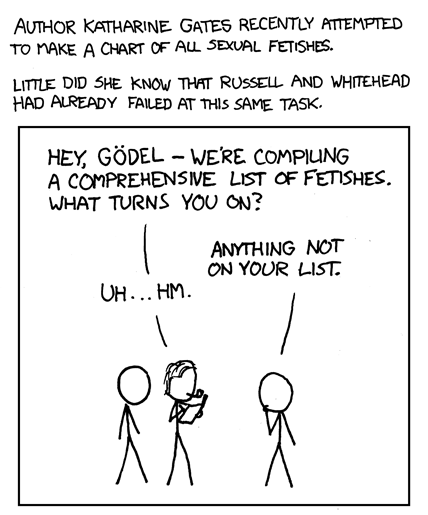
\includegraphics[height=5cm]{background/pix/xkcdfetishes.png}  \\
        \protect\label{fig:xkcdfetishes}\protect\href{https://xkcd.com/468/}{Courtesy XKCD}
      \protect\end{tabular}
    \protect\end{center}
  } % end boolean MakingPaperCopy
}。
\begin{equation*}
  R=\set{s \suchthat s\notin f(s)}
\end{equation*}
我们将证明定义域中没有元素映射到~$R$，因此 $f$ 不是满射。
假设存在 $\hat{s}\in S$ 使得 $f(\hat{s})=R$。
考虑 $\hat{s}$ 是否是~$R$ 的元素。
我们有 $\hat{s}\in R$ 当且仅当 $\hat{s}\in\set{s\suchthat s\notin f(s)}$。
根据~$R$ 的定义，这成立当且仅当 $\hat{s}\notin f(\hat{s})$，而这
又当且仅当 $\hat{s}\notin R$ 时成立。
这一矛盾意味着这样的 $\hat{s}$ 不存在。
\end{proof}


%</pf:CantorsThm>

%<*cor:FcnsNToNNotCountable>


\begin{corollary} \label{cor:FcnsNNGreaterFcnsN}
自然数集~$\N$ 的势严格小于自然数函数集~$\map{f}{\N}{\N}$ 的势。
也就是说，这样的函数有不可数多个。
\end{corollary}


%</cor:FcnsNToNNotCountable>

%<*pf:FcnsNToNNotCountable>


\begin{proof}
记函数集为~$G$。
存在一个从 $\powerset(\N)$ 到~$G$ 的一一映射，即把
每个子集 $S\subseteq\N$ 与其特征函数 $\map{\charfcn{S}}{\N}{\N}$ 相关联的映射。
因此 $\sizeof{\N}<\sizeof{\powerset(\N)}\leq\sizeof{G}$。
\end{proof}


%</pf:FcnsNToNNotCountable>

\begin{corollary}[不可计算函数的存在性]
存在一个函数 $\map{f}{\N}{\N}$，它不是可计算的：对所有~$e$，$f\neq\TMfcn_e$。
\end{corollary}

\begin{proof}
固定一个字母表。\footnotemark{} %
\zcref{co:SetOfTMsCountable}
表明，在这个字母表上，Turing 机是可数多的。
先前的结论表明，从 $\N$ 到自身的函数是不可数多的。
因此，Turing 机严格少于从 $\N$ 到自身的函数。
特别地，如果我们把每台 Turing 机与它计算的函数关联起来，
这个关联不是满射。
所以，存在一个自然数函数，没有 Turing 机能计算它。
\end{proof}

\footnotetext{%
  我们可以使用任意一个至少包含一个除空白符外字符的字母表，
  例如 $\Sigma=\set{\blank,\str{1}}$。
  在 Church 论题的讨论中，我们陈述过（尽管没有证明）
  在这种字母表上的 Turing 机能计算任何在其他字母表上可计算的函数。}

这是一个划时代的结果。
根据 Church 论题，\index{Church's Thesis!and uncountability}
我们以此证明存在一些计算机无法完成的工作。

%\footnote{%
  对于上过程序设计课的人来说，他们反复经历从任务到完成该任务的程序的转换，
  存在无法完成的事情可能令人惊讶，甚至震惊。
  这些结果的一个要点是，尽管这里关于无穷大小的工作
  起初可能显得过于抽象而不切实际，
  但它仍然能得出有趣且有用的结论。
%}

% ...............................................
\begin{exercises}


\begin{exercise}
\citetext{你的学习伙伴对对角化论证感到困惑}{%
  来自 \autocite{SE:Kaktus}.}。
  “如果你有一个无限长的列表，它显然包含所有的数字，对吧？
  我的意思是，如果你有一个真正‘无限’的列表，
  那你根本不可能找到一个不在列表上的数字！”
  帮他们理清思路。
\begin{answer}\verified
无限与穷尽是两回事。
列表 $0,2,4,\ldots$ 是无限的，但并没有穷尽所有自然数。
\end{answer}
\end{exercise}

\begin{exercise}
你的同学说：“教授，我搞糊涂了。
有一位小数的数构成的集合，比如 $25.4$ 和 $0.1$，显然是可数的——只需将整数的小数点全部左移一位即可。
有两位小数的集合，比如 $2.54$和 $6.02$，同样可数，以此类推。
这是可数多个集合，每个都可数，所以它们的并集是可数的。
这个并集就是全体实数，所以我认为实数是可数的。”
他们的错误在哪里？
\begin{answer}\verified
  这个并集并不是全体实数。
  它不包含无理数。
  例如，$\pi=3.14\ldots{}$ 不在任何一个集合中，因此也不在并集中。
  你的同学只考虑了末尾为零的数。
\end{answer}
\end{exercise}

\begin{exercise}
对下列有限集验证 Cantor 定理（\zcref{th:CantorsThm}）。
\begin{exparts*}
\item $\set{0,1,2}$
\item $\set{0,1}$
\item $\set{0}$
\item $\set{}$
\end{exparts*}
\begin{answer}\verified
Cantor 定理说幂集的元素个数比原集合多。
\begin{exparts}
\item 集合 $\set{0,1,2}$ 有三个元素，
它的幂集有八个元素。
\begin{equation*}
  \powerset(\set{0,1,2})=
  \set{\set{0,1,2},\; \set{0,1},\; \set{0,2},\; \set{1,2},\;
       \set{0},\; \set{1},\; \set{2},\; \emptyset}
\end{equation*}
\item 集合 $\set{0,1}$ 有两个元素，而它的幂集
$\powerset(\set{0,1})=\set{\set{0,1},\set{0},\set{1},\emptyset}$
有四个元素。
\item 集合 $\set{0}$ 只有一个元素，但它的幂集
$\powerset(\set{0})=\set{\set{0},\emptyset}$ 有两个元素。
\item 空集有零个元素，而它的幂集
$\powerset{\emptyset}=\set{\emptyset}$ 有一个元素。
\end{exparts}
\end{answer}
\end{exercise}

\recommended


\begin{exercise}
使用 \zcref{def:CardLessThanOrEqual} 证明第一个集合的势小于或等于第二个集合。
\begin{exparts}
\item $S=\set{1,2,3}$，$\hat{S}=\set{11,12, 13}$
\item $T=\set{0,1,2}$，$\hat{T}=\set{11,12, 13, 14}$
\item $U=\set{0,1,2}$，奇数集合
\item 偶数集合，奇数集合
\end{exparts}
\begin{answer}\verified
势的“$\leq$”定义是：如果存在一个从 $A$ 到~$B$ 的一一函数，
则 $\sizeof{A}\leq\sizeof{B}$。
\begin{exparts}
\item 函数 $\map{f}{S}{\hat{S}}$ 定义为 $f(1)=11$，$f(2)=12$，
$f(3)=13$，通过观察可知它是一一的。
\item 函数 $\map{f}{T}{\hat{T}}$ 定义为 $f(1)=11$，$f(2)=12$，
$f(3)=13$，通过观察可知它是一一的。
\item 同样通过观察，
函数 $\map{f}{U}{\mathbb{O}}$ 定义为 $f(1)=1$，$f(2)=3$，
$f(3)=5$，它是一一的。
\item
函数 $\map{f}{\mathbb{E}}{\mathbb{O}}$ 定义为 $f(x)=x+1$ 是一个一一函数。
验证很容易：$f(x_0)=f(x_1)$ 蕴含 $x_0+1=x_1+1$，
所以 $x_0=x_1$。
\end{exparts}
\end{answer}
\end{exercise}

\begin{exercise}
一个集合是可数的，另一个是不可数的。
哪个是哪个？
\begin{exparts*}
\item $\set{n\in\Z\suchthat n+3< 5}$
\item $\set{x\in\R\suchthat x+3< 5}$
\end{exparts*}
\begin{answer}
两者的区别在于元素所取自的集合不同。
\begin{exparts}
\item 集合 $S=\set{n\in\Z\suchthat n+3< 5}=\set{\ldots,-2,-1,0,1}$
  是可数的。
  由 $n\mapsto -n+1$ 定义的函数 $\map{f}{\N}{S}$ 是一个对应，这很容易验证。
\item 不可数；它是实数集 $\open{-\infty}{2}$。
  （在映射 $x\mapsto \ln(2-x)$ 下，此集合与 $\R$ 对应。）
\end{exparts}
\end{answer}
\end{exercise}

\recommended


\begin{exercise}
指出每个集合是可数的还是不可数的。
只需用一个词回答。
\begin{exparts*}
\item
$\open{5}{\infty}\subset\R$
\item
$\leftclosed{1}{4}\subset\N$
\item
$\leftclosed{1}{4}\subset\R$
\item
$\leftclosed{5}{\infty}\subset\N$
\end{exparts*}
\begin{answer}\verified
\begin{exparts}
\item 不可数。
  （函数 $x\mapsto\ln(x-5)$ 是与 $\R$ 的一个对应。）
\item 可数。
  （因为它是作为自然数的子集给出的，而且该集合是 $\set{1,2,3}$，是有限的。）
\item 此集合是不可数的。
  （集合 $S=\leftclosed{1}{4}\subset\R$ 的势至少与 $T=\open{1}{4}\subset\R$ 相同，
  因为由 $x\mapsto x$ 给出的包含映射 $\map{\iota}{T}{S}$ 是一一的。
  区间 $T$ 与 $\R$ 同势。
  一种理解方式是，从区间 $\open{-\pi/2}{\pi/2}$ 与 $\R$ 之间由 $x\mapsto \tan(x)$ 给出的对应出发。
  通过将该区间按 $\pi/3$ 的比例缩放然后再平移，使其适配定义域 $T$ 的情况，可得
  $x\mapsto \tan(\,(\pi/3)\cdot(x-1)-(\pi/2)\,)$ 是一个对应。）
\item 可数。
  （$\N$ 的任何子集都是可数的。）
\end{exparts}
\end{answer}
\end{exercise}

\begin{exercise}
列出所有定义域为 $A_2=\set{0,1}$、陪域为 $\powerset(A_2)$ 的函数。
对于一个有三个元素的集合 $A_3$，有多少个这样的函数？
$n$~个元素呢？
\begin{answer}\verified
对于二元集 $A_2=\set{0,1}$，其幂集，
$\powerset(A_2)=\set{\set{0,1},\, \set{0}, \set{1}, \set{}}$，
有四个元素。
构造一个从 $A_2$ 到 $\powerset(A_2)$ 的函数，需要指定将 $0$ 和 $1$ 映射到哪里。
因此有 $4^2=16$ 个不同的函数。
\begin{equation*}
\begin{array}{r|*{2}{c}}
  \multicolumn{1}{r}{\tabulartext{function~$f_i$}}
         &f_i(0)     &f_i(1)  \\
  \hline
  f_{0}  &\set{}     &\set{}  \\
  f_{1}  &\set{}     &\set{0}  \\
  f_{2}  &\set{}     &\set{1}  \\
  f_{3}  &\set{}     &\set{0,1}  \\
  f_{4}  &\set{0}    &\set{}  \\
  f_{5}  &\set{0}    &\set{0}  \\
  f_{6}  &\set{0}    &\set{1}  \\
  f_{7}  &\set{0}    &\set{0,1}  \
\end{array}
\hspace*{3em}
\begin{array}{r|*{2}{c}}
  \multicolumn{1}{r}{\tabulartext{function~$f_i$}}
         &f_i(0)     &f_i(1)  \\
  \hline
  f_{8}  &\set{1}    &\set{}  \\
  f_{9}  &\set{1}    &\set{0}  \\
  f_{10} &\set{1}    &\set{1}  \\
  f_{11} &\set{1}    &\set{0,1}  \\
  f_{12} &\set{0,1}  &\set{}  \\
  f_{13} &\set{0,1}  &\set{0}  \\
  f_{14} &\set{0,1}  &\set{1}  \\
  f_{15} &\set{0,1}  &\set{0,1}  \\
\end{array}
\end{equation*}

三元集 $A_3$ 有
$\sizeof{\powerset(A_3)}=8$。
从 $A_3$ 到 $\powerset(A_3)$ 的函数数量是 $8^3=512$。
一般而言，当 $\sizeof{A}=n$ 时，幂集有
$\sizeof{\powerset(A_3)}=2^n$ 个元素。
函数数量是 $(2^n)^n=2^{(n^2)}$。
（作为验证，$n=2$ 得到 $2^4=16$，
$n=3$ 得到 $2^9=512$。）
\end{answer}
\end{exercise}

\begin{exercise}
列出所有从 $S$ 到 $T$ 的函数。
哪些是一一的？
\begin{exparts*}
\item $S=\set{0,1}$, $T=\set{10,11}$
\item $S=\set{0,1}$, $T=\set{10,11,12}$
\end{exparts*}
\begin{answer}\verified
\begin{exparts}
\item 这些是从 $S$ 到 $T$ 的函数。
  \begin{equation*}
  \begin{array}{r|*{2}{c}}
    \multicolumn{1}{c}{\tabulartext{function $f_i$}}
          &f_i(0)  &f_i(1)  \\
    \cline{2-3}
    f_{0} &10      &10 \\
    f_{1} &10      &11 \\
    f_{2} &11      &10 \\
    f_{3} &11      &11 \\
  \end{array}
  \end{equation*}
  一一的函数是 $f_1$ 和 $f_2$。
\item 这些是从 $S$ 到 $T$ 的函数。
  \begin{equation*}
  \begin{array}{r|*{2}{c}}
    \multicolumn{1}{c}{\tabulartext{function $f_i$}}
          &f_i(0)  &f_i(1)  \\
    \hline
    f_{0} &10       &10 \\
    f_{1} &10       &11 \\
    f_{2} &10       &12 \\
    f_{3} &11       &10 \\
    f_{4} &11       &11 \\
  \end{array}
  \hspace{3em}
  \begin{array}{r|*{2}{c}}
    \multicolumn{1}{c}{\tabulartext{function $f_i$}}
          &f_i(0)  &f_i(1)  \\
    \hline
    f_{5} &11       &12 \\
    f_{6} &12       &10 \\
    f_{7} &12       &11 \\
    f_{8} &12       &12 \\
  \end{array}
  \end{equation*}
  一一的函数是 $f_1$、$f_2$、$f_3$、$f_5$、$f_6$
  和 $f_7$。
\end{exparts}
\end{answer}
\end{exercise}

\recommended


\begin{exercise}\begin{credit}
  \href{http://scherk.pbworks.com/w/page/14864221/Quiz%3A%20Countable%20sets}{User scherk at \texttt{pbworks.com}}.
\end{credit}
简答题：填空，从下列选项中选择可能的最强结论填入每个空格，
(i)~不可数，
(ii)~可数或不可数，
(iii)~有限，
(iv)~可数，
(v)~有限、可数无限或不可数
（同一答案可用于多个空格或完全不用）。
无需给出证明。
\begin{exparts}
\item 如果 $A$ 和 $B$ 是有限的，
那么 $A\cup B$ 是 \fillinblank。
\item 如果 $A$ 是可数的且 $B$ 是有限的，
那么 $A\cup B$ 是 \fillinblank。
\item 如果 $A$ 是可数的且 $B$ 是不可数的，
那么 $A\cup B$ 是 \fillinblank。
\item 如果 $A$ 是可数的且 $B$ 是不可数的，
那么 $A\cap B$ 是 \fillinblank。
\end{exparts}
\begin{answer}\verified
\begin{exparts}
\item 答案是~(iii)~有限，因为两个有限集的并集是有限的。
  （以下所有选项都成立：(ii)~可数或不可数，
  (iii)~有限，
  (iv)~可数，
  以及 (v)~有限、可数无限或不可数。
  但最强、最具体的是~(iii)。）
\item 最强的是~(iv)。
\item 最强的是~(i)。
\item 最强的是~(iv)。
  （交集可能是有限的，但也存在可数的情况，例如 $A=\N$ 和 $B=\R$。
  因此在一般情况下我们能做出的最强陈述是~(iv)。）
\end{exparts}
\end{answer}
\end{exercise}

\begin{exercise}
简答题：考虑 $\map{f}{S}{T}$，其中 $S$ 是可数的。
对于以下两项，列出所有可能成立的选项
(i)~$S$ 是有限的，
(ii)~$T$ 是有限的，
(iii)~$S$ 是可数无限的，
(iv)~$T$ 是可数无限的，
(v)~$T$ 是不可数的：
\begin{exparts*}
\item 该映射是满射的，
\item 该映射是一一的。
\end{exparts*}
\begin{answer}\verified
问题不要求证明，但这里的括号注释给出了理由。
\begin{exparts}
\item
  除最后一项外，其他都是可能的。
  （满足 (i) 和 (ii) 的一个例子是 $\map{\identity}{\set{0,1}}{\set{0,1}}$。
  满足 (iii) 和 (iv) 的一个例子是 $\map{\identity}{\N}{\N}$。
  \zcref{lem:CountableIffOntomap} 排除了 (v)。）
\item
  所有都是可能的。
  （满足 (i) 和 (ii) 的一个例子是 $\map{\identity}{\set{0,1}}{\set{0,1}}$。
  满足 (iii) 和 (iv) 的一个例子是 $\map{\identity}{\N}{\N}$。
  满足 (v) 的一个例子是由 $\iota(x)=x$ 给出的 $\map{\iota}{\N}{\R}$。）
\end{exparts}
\end{answer}
\end{exercise}

\begin{exercise}
\begin{credit}
   Math StackExchange 用户 Robert Z \url{https://math.stackexchange.com/a/1896328/12012}
\end{credit}
设 $S=\closed{0}{1}$ 和 $T=\open{0}{1}$ 是实数区间。
给出一个对应。
\hint~$f(x)=x$ 对大多数输入都有效，但端点必须映射到某个位置，所以
从 $f(0)=1/2$ 和 $f(1)=1/4$ 开始，并顺推下去。
\begin{answer}\verified
根据提示，考虑以下函数。
\begin{display}
  \begin{minipage}{0.5\textwidth}
    \begin{equation*}
      f(x)=
      \begin{cases}
        1/2  &\case{if $x=0$}  \\
        1/2^{n+2}  &\case{if $x=1/2^n$ for $n\in\N$}  \\
        x    &\case{otherwise}
      \end{cases}
    \end{equation*}
  \end{minipage}
  \quad
  \vcenteredhbox{
\includegraphics{\asydir correspondences/correspondences005.pdf}}
\end{display}
论证函数 $f$ 是一一的且满射的一种方法是看它满足水平线测试，
即对于每个 $t\in\open{0}{1}$，水平线 $y=t$ 都恰好有一个对应的输入 $x$。

我们可以展开说明。
首先考虑输出 $y\in\open{0}{1}$ 满足 $y\neq 1/2^n$（$n\in\N^+$）的情况。
那么 $y$ 恰好有一个对应的输入，即 $x=y$。
另一种情况是对某个 $n\in\N^+$ 有 $y=1/2^n$。
这里也有且仅有一个对应的输入 $x$。
具体来说，如果 $n=1$，那么输入是 $x=0$，它在定义域
$\closed{0}{1}$ 中。
如果 $n> 1$，那么输入是 $x=1/2^{n-2}$，它也是 $\closed{0}{1}$ 中的一个元素。
\end{answer}
\end{exercise}

\recommended


\begin{exercise}
给出一个势大于 $\R$ 的集合。
\begin{answer}\verified
\zcref{th:CantorsThm} 说对于任意集合，
其势严格小于其幂集的势。
所以一个势大于 $\R$ 的集合是 $\powerset(\R)$。
（另一个是 $\powerset(\powerset(\R))$。）
\end{answer}
\end{exercise}

\recommended


\begin{exercise}
回忆我们将比特的集合记为 $\B=\set{0,1}$。
\begin{exparts}
\item
证明有限比特串的集合，
$\sequence{b_0b_1\ldots\, b_{k-1}}$（其中 $b_i\in\B$ 且 $k\in\N$），
是可数的。
\item
我们可以将无限比特串 $f=\sequence{b_0,b_1,\ldots}$ 视为函数 $\map{f}{\N}{\B}$。
使用对角化证明无限比特串的集合
是不可数的。
\end{exparts}
\begin{answer}\verified
\begin{exparts}
\item 有限比特串的集合 $\kleenestar{\B}\!$，是集合
  $\B^k=\set{\sequence{b_0b_1\ldots\, b_{k-1}}\suchthat k\in\N}$ 的并集。
  集合 $\B^k$ 是有限的，因为它有 $2^k$~个元素
  （当 $k=0$ 时，它只包含空串），所以
  这是可数多个可数集合的并集。
\item
  假设我们可以对无限比特串的集合进行计数，
  即它有一个穷举枚举 $f_0, f_1, \ldots$\sentencespace
  令 $\map{g}{\B}{\B}$ 由 $g(0)=1$ 和
  $g(1)=0$ 给出。
  那么由 $F(i)=g(f_i(i))$ 定义的无限比特串 $\map{F}{\N}{\B}$ 不等于
  任何一个 $f_i$，
  这与该枚举是穷举的相矛盾。
\end{exparts}
\end{answer}
\end{exercise}

\begin{exercise}
证明对于两个集合，$S\subseteq T$ 蕴含 $\sizeof{S}\leq \sizeof{T}$。
\begin{answer}\verified
设 $S$ 和 $T$ 满足 $S\subseteq T$。
那么包含映射，即由 $\iota(s)=s$ 给出的映射 $\map{\iota}{S}{T}$，
显然是一一的。
所以由 \zcref{def:CardLessThanOrEqual}，$\sizeof{S}\leq \sizeof{T}$。
\end{answer}
\end{exercise}

\begin{exercise}
用对角化方法证明以下命题为假：所有值域有限的函数~$\map{f}{\N}{\N}$ 都是可计算的。
\hint~只需证明这类函数的集合是不可数的。
\begin{answer}\verified
我们遵照提示。
将所有这样的函数组成的集合记作$S=\set{\map{f}{\N}{\N}\suchthat \text{$\range(f)$ is finite}}$。
假设 $S$ 是可数的，从而存在一个对应 $\map{h}{\N}{S}$。
对于所有自然数~$i$，$h(i)$ 的值是一个函数，我们将其记作~$f_i$。

定义映射 $\map{g}{\N}{\N}$：若 $x\neq 0$ 则 $g(x)=0$，否则 $g(x)=1$。
考虑由$k(i)=g(\,f_i(i)\,)$给出的函数 $\map{k}{\N}{\N}$。
这个映射的值域是有限的，即$\range(k)=\set{0,1}$，但 $k$ 不等于 $S$ 中的任何一个~$f_i$，因为它们在输入~$i$ 处的取值不同。
\end{answer}
\end{exercise}

% \begin{exercise}
% Given a countable number of nonempty sets, $S_i\neq\emptyset$ for
% $i\in\N$,
% show that their product
% $S_0\times S_1\times \cdots$ is uncountable.
% \begin{answer} % Requires countable choice https://math.stackexchange.com/a/500855
% Let $T=S_0\times S_1\times \cdots$ where each $S_i$ is nonempty.
% Clearly $T$ is infinite.
% We will show that no map $\map{f}{\N}{T}$ is onto.

% Recall that the characteristic function of $S_i$ is denoted $\charfcn(S_i)$.
% Let $g$ be the map on $\B=\set{0,1}$ given by
% $g(b)=1-b$, which is $g(0)=1$ and $g(1)=0$.

% Now consider the set whose characteristic function is
% $g(\charfcn(S_i)(i))$.
% Then for all~$i$, $z\neq f(i)$ because $z[i]\neq f(i)[i]$.
% So $f$ is not onto.
% \end{answer}
% \end{exercise}

% No way to make an exercise? https://math.stackexchange.com/a/183383/12012
% \begin{exercise}
% You study with someone who says,
% ``Yes, obviously there are different sizes of infinity.
% The plane $\R^2$ obviously has infinitely many more points then the
% line~$\R$, so it is a larger infinity.''
% Convince them that
% their argument is wrong because the cardinality of the plane is the same
% as the cardinality of the line.
% \hint~consider the function $\map{f}{\R^2}{\R}$ such that $f(x,y)$ interleaves
% the digits of the two input numbers.
% \end{exercise}

\begin{exercise}
在数学课上，我们主要处理有理数，这可能给人留下无理数不常见的印象。
但实际上，无理数比有理数更多。
证明：根据 \zcref{ex:RationalsAreCountable}，虽然有理数集是可数的，但无理数集是不可数的。
\begin{answer}\verified
\zcref{ex:RationalsAreCountable} 表明有理数集是可数的。
假设无理数集也是可数的。
那么由于两个可数集的并集是可数的，实数集将是可数的。
但实数集是不可数的，因此无理数集也不可数。
\end{answer}
\end{exercise}

\recommended


\begin{exercise}
\zcref{ex:RationalsAreCountable} 表明有理数是可数的。
如果我们将 \zcref{th:RealsNotCountable} 中给出的对角线论证应用到有理数的一个枚举上，会发生什么？
考虑一个包含所有有理数的序列 $q_0, q_1,\ldots$。
用小数展开式 $q_i=d_i.d_{i,0}d_{i,1}d_{i,2}\ldots$（其中 $d_i\in\Z$ 且$d_{i,j}\in\set{0,\ldots 9}$）表示每个这样的数，该展开式不以全~$9$ 结尾，从而保证小数展开式是唯一的。
\begin{exparts}
\item
  设 $g$ 是定义在十进制数字 $0,1,\ldots{} 9$ 上的映射，满足 $g(1)=2$，且当 $i\neq 2$ 时 $g(i)=1$。
  考虑对角线上的数$d=\sum_{n\in\N}d_{n,n}\cdot 10^{-(n+1)}\!$。
  用~$g$ 变换其各位数字，即定义$z=\sum_{n\in\N}g(d_{n,n})\cdot 10^{-(n+1)}\!$。
  证明 $z$ 是无理数。
\item 利用前一小题得出结论：对角线上的数 $d=\sum_{n\in\N}d_{n,n}\cdot 10^{-(n+1)}$ 是无理数。
  \hint~证明它的小数展开式没有重复模式。
\item
  为什么对角线上的数不是有理数这一事实，与我们能够枚举所有有理数这一事实不矛盾？
\end{exparts}
\begin{answer}\verified
\begin{exparts}
\item
  将 $z$ 的小数展开式写成~$z=0.z_0z_1z_2\ldots$\sentencespace
  由于 $g$ 的输出永远不会是~$9$，所以 $z$ 的小数展开式不以 $9$ 结尾。
  因此 $z$ 有唯一的小数展开式。
  对于每个~$q_i$，$z$ 的小数展开式与 $q_i$ 的不同之处在于$z_{i}\cdot 10^{-(i+1)}\neq q_{i,i}\cdot 10^{-(i+1)}$，
  这是由~$g$ 的定义决定的。
  因为它们的小数展开式不同，并且都不以 $9$ 结尾，所以它们是不同的数。

  由于 $z$ 不等于任何有理数，所以它是无理数。
\item
  如果$d=\sum_{n\in\N}d_{n,n}\cdot 10^{-(n+1)}$是有理数，那么它的小数展开式会循环。
  也就是说，存在一个小数位，使得从该位之后，展开式由一串数字$d_{j}d_{j+1}\ldots\, d_{j+k}$不断重复组成。
  但这样一来，前一小题中的~$z$ 也会循环，即从同一个小数位之后，它的展开式将由一串数字$g(d_{j})g(d_{j+1})\ldots\, g(d_{j+k})$不断重复组成。
  这将使得~$z$ 成为有理数，但 $z$ 并不是。
\item
  在 \zcref{th:RealsNotCountable} 中，我们从一个声称包含所有实数的列表开始，然后构造出一个不在该列表中的实数。
  这里，我们从一个包含所有有理数的列表开始，构造出了一个不是有理数的数。
  这使得它仍然是一个实数，只不过不是有理实数。
\end{exparts}
\end{answer}
\end{exercise}

\begin{exercise}
通过证明若 $S$ 有限，则其幂集的势是 $\sizeof{\powerset(S)}=2^{\sizeof{S}}$，来验证 Cantor 定理在有限情况下成立。
\begin{answer}\verified
在证明之前，作为归纳步骤的启发，考虑 $S=\set{0,1,2,3}$。
这些是 $\powerset(S)$ 的十六个元素。
第一行是不包含~$3$ 的集合，而第二行是包含~$3$ 的集合。
\begin{equation*}
\begin{array}{*{8}{c}}
  \set{},  &\set{0},   &\set{1},   &\set{2},   &\set{0,1},   &\set{0,2},   &\set{1,2},   &\set{0,1,2}, \\
  \set{3}, &\set{0,3}, &\set{1,3}, &\set{2,3}, &\set{0,1,3}, &\set{0,2,3}, &\set{1,2,3}, &\set{0,1,2,3}
\end{array}
\end{equation*}
底行的每个集合与顶行匹配的集合相同，只是多加了一个~$3$。

我们通过对 $\sizeof{S}$ 进行归纳来证明。
基本情况是 $\sizeof{S}=0$，即 $S$ 是空集。
那么 $\powerset(S)=\set{\emptyset}$ 且 $\sizeof{\powerset(S)}=1=2^0\!$，符合要求。

对于归纳步骤，固定 $k\in\N^+\!$，假设命题对 $n=0$，$n=1$，\ldots{} $n=k$ 成立，并考虑一个集合 $S$ 满足 $\sizeof{S}=k+1$。
因为 $\sizeof{S}=k+1$，集合~$S$ 至少有一个元素 $\hat{s}\in S$。
对 $S-\set{\hat{s}}$ 应用归纳假设可知，$\powerset(S-\set{\hat{s}})$ 有 $2^k$ 个元素。
如上所示，$\powerset(S)$ 中不包含 $\hat{s}$ 的元素与 $\powerset(S)$ 中包含~$\hat{s}$ 的元素一一对应。
但是 $\powerset(S)$ 中不包含~$\hat{s}$ 的集合正是 $\powerset(S-\set{\hat{s}})$ 中的集合。
因此，$\powerset(S)$ 的元素总数是 $2\cdot 2^k$，等于 $2^{k+1}\!$。
\end{answer}
\end{exercise}

\begin{exercise}
\begin{credit}
  \href{https://viterbi-web.usc.edu/~mjneely/docs/infinity.pdf}{Michael J~Neely }
\end{credit}
\zcref{th:RealsNotCountable} 中 Cantor 定理证明的关键是 $R=\set{s\suchthat s\notin f(s)}$ 的定义。
这个故事阐明了这个思想：高中年鉴要求每个毕业生~$s_i$ 列出一个他们认为将来会成名的班级成员名单 $f(s_i)$。
定义谦逊学生集合~$H$ 由那些不在自己名单上的学生组成。
证明没有学生的名单等于~$H$。
\begin{answer}\verified
假设 $f(s_i)=H$。
我们将论证 $s_i\in H$ 和 $s_i\notin H$ 都不成立。
如果 $s_i\in H$，那么学生~$s_i$ 是自己名单上的一员，因此根据谦逊的定义，$s_i$ 不谦逊，这与该情况下的假设矛盾。
另一方面，如果 $s_i\notin H$，那么 $s_i$ 不在自己名单上，因此 $s_i$ 是谦逊的，这与该情况下的假设矛盾。
\end{answer}
\end{exercise}

\begin{exercise}
证明不存在所有集合的集合。
\hint~使用 \zcref{th:CantorsThm}。
\begin{answer}\verified
  假设相反，即 $\mathcal{C}$ 是所有集合的集合。
  那么 $\powerset(\mathcal{C})$ 将是一个集合的集合，因此我们将有 $\powerset(\mathcal{C})\subseteq \mathcal{C}$。
  这将导致 $\sizeof{\powerset(\mathcal{C})}\leq\sizeof{\mathcal{C}}$，从而与 Cantor 定理矛盾。
\end{answer}
\end{exercise}

\begin{exercise}
\zcref{th:RealsNotCountable} 的证明必须处理某些十进制数有不止一种表示的事实。
二进制也具有某些数不止一种表示的性质；例如 $0.01000\ldots$ 和 $0.00111\ldots$。
但在二进制的论证中，构造~$z$ 时无法避免数字~$0$ 和~$1$。
如何使该论证在二进制下成立？
\begin{answer}\verified
一种方法是每次取两个对角线位；例如将 $01$ 改为 $10$，并将任何其他两位序列改为 $01$。
\end{answer}
\end{exercise}

\begin{exercise}
\begin{credit}
  答案由 Stack Exchange 用户\footnote{\url{https://math.stackexchange.com/a/271126}} Alex Becker 提供。
\end{credit}
在 \zcref{th:RealsNotCountable} 的陈述之后的讨论中提到，实数~$1$ 有两种小数表示：$1.000\ldots=0.999\ldots$\sentencespace
\begin{exparts}
\item
使用无限几何级数的公式验证这个等式，$a+ar+ar^2+ar^3+\cdots =a/(1-r)$。
\item
证明如果一个数有两种不同的小数表示，那么在它们最左边不同的那个小数位上，它们的数字恰好相差~$1$。
\hint 提示：余下的小数位所能弥补的最大差值就是这个数。
\item
此外，证明在首次不同的数位上数字较大的那种表示中，其右边所有数位上的数字都是~$0$；而另一种表示中，所有余下数位上的数字都是~$9$。% \hint~this is similar to the prior item.
\end{exparts}
\begin{answer}\verified
在这个原型 $1.000\ldots=0.999\ldots$ 中，我们将两种表示写作
$x_0=1$，$x_{-1}=0$，$x_{-2}=0$，……，和
$y_0=0$，$y_{-1}=9$，$y_{-2}=9$，……\sentencespace
注意，这些下标（即小数位）是像 $0$ 和~$-1$ 这样的整数，并非自然数。
\begin{exparts}
\item
在$a+ar+ar^2+ar^3+\cdots =a/(1-r)$中，令 $a=9$ 且 $r=0.1$。
左边是$9+0.9+0.09+0.009+\cdots=9.999\,99\ldots$\sentencespace
右边是$9/(1-(0.1))=9/0.9=10$。
两边减去~$9$ 可得 $0.999\,99\ldots=1$。
\item
考虑一个有两种表示的实数。
在这两种表示中存在一个最左边的非零小数位 $N\in\Z$。
因此，将这两种表示写为$\vec{x}=\sequence{x_N,x_{N-1},\ldots}$ 和
$\vec{y}=\sequence{y_N,y_{N-1},\ldots}$。
它们需要满足条件$x_i,y_i\in\set{0,1,\ldots 9}$，并且加起来等于同一个数。
\begin{equation*}
  \sum_{i\leq N}x_i\cdot 10^i=\sum_{i\leq N}y_i\cdot 10^i
  \tag{$*$}
\end{equation*}

将 ($*$) 改写成差值形式。
\begin{equation*}
  0=\bigl(\sum_{i\leq N}x_i\cdot 10^i\bigr)-\bigl(\sum_{i\leq N}y_i\cdot 10^i\bigr)
   =\sum_{i\leq N}(x_i-y_i)\cdot 10^i
\end{equation*}
设 $\vec{x}$ 和 $\vec{y}$ 首次不同的最左小数位为第~$M$ 位，
即对于 $i\in\set{N,N-1,\ldots\, M+1}$ 有 $x_i=y_i$，且 $x_M\neq y_M$。
$x_M$ 和~$y_M$ 其中一个大；不妨设 $x_M>y_M$。
去掉前面的零后，现在差值从第 $M$ 位开始。
\begin{equation*}
  0
   =\sum_{i\leq M}(x_i-y_i)\cdot 10^i
   =(x_M-y_M)\cdot 10^M+\sum_{i\leq (M-1)}(x_i-y_i)\cdot 10^i
  \tag{$**$}
\end{equation*}
我们在等式右边单独列出了第一项，因为我们需要证明 $x_M=y_M+1$
（正如原型中$\vec{x}=\sequence{1,0,0,\ldots}$和
$\vec{y}=\sequence{0,9,9,\ldots}$的情况那样）。
考虑余下的部分，$\sum_{i\leq (M-1)}(x_i-y_i)\cdot 10^i\!$。
为了使总和为零，这个尾部必须抵消$(x_M-y_M)\cdot 10^M\!$，
由于 $x_M>y_M$，这是一个正值。
尾部所能提供的最大抵消量出现在每个 $x_i-y_i$ 都等于~$-9$ 时。
几何级数公式给出了这个最大值。
\begin{equation*}
  -9\cdot 10^{M-1}-9\cdot 10^{M-2}+\cdots
  =-9\cdot 10^{M-1}\cdot\bigl[ 1+\frac{1}{10}+\frac{1}{100}+\cdots\bigr]  \\
  =\frac{-9\cdot 10^{(M-1)}}{1-(1/10)}=\frac{-9\cdot 10^{(M-1)}}{9/10}=-10^{M}
\end{equation*}
因此 $x_M-y_M=1$，因为尾部无法抵消更大的差值。
\item
再次考虑上一项的 ($**$)，既然我们已经证明了 $x_M-y_M=1$。
\begin{equation*}
  0
   =1\cdot 10^M+\sum_{i\leq (M-1)}(x_i-y_i)\cdot 10^i
\end{equation*}
我们想要证明每个 $x_i-y_i$ 都等于~$-9$。
我们只处理 $i=M-1$ 的情况，因为其他情况与此非常类似。

如果$x_{M-1}-y_{M-1}\geq -8$，那么 ($**$) 变为：
\begin{align*}
  0
   &=1\cdot 10^M+(x_{M-1}-y_{M-1})\cdot 10^{(M-1)}+\sum_{i\leq (M-2)}(x_i-y_i)\cdot 10^i
     \\
   &\geq 10\cdot 10^{(M-1)}-8\cdot 10^{(M-1)}+\sum_{i\leq (M-2)}(x_i-y_i)\cdot 10^i \\
   &=2\cdot 10^{(M-1)}+\sum_{i\leq (M-2)}(x_i-y_i)\cdot 10^i
\end{align*}
与上一项类似，为了使整个和为负，尾部必须抵消第一项。
通过令每个 $x_i-y_i$ 为 $-9$，可以得到最大的尾部。
再次应用无限几何级数的求和公式。
\begin{equation*}
  -9\cdot 10^{M-2}-9\cdot 10^{M-3}+\cdots
  =-9\cdot 10^{M-2}\cdot\bigl[ 1+\frac{1}{10}+\frac{1}{100}+\cdots\bigr]  \\
  =\frac{-9\cdot 10^{(M-2)}}{1-(1/10)}=\frac{-9\cdot 10^{(M-2)}}{9/10}=-10^{M-1}
\end{equation*}
尾部不足以抵消$2\cdot 10^{(M-1)}$，所以
$x_{M-1}-y_{M-1}\geq -8$ 是不可能的。
\end{exparts}
\end{answer}
\end{exercise}

\begin{exercise} \label{exer:SchroderBernstein}
\zcref{def:CardLessThanOrEqual} 将等势的定义推广为：如果存在从 $A$ 到 $B$ 的一一函数，则 $\sizeof{A}\leq \sizeof{B}$。
\definend{Schröder–Bernstein 定理} 指出，如果同时有 $\sizeof{S}\leq \sizeof{T}$ 和 $\sizeof{T}\leq \sizeof{S}$，那么 $\sizeof{S}=\sizeof{T}$。
我们将逐步讲解这个证明。
它依赖于寻找像的链：对于任意 $s\in S$，我们通过反复应用这两个函数（既向右也向左）来形成与之关联的链，如下所示。
\begin{equation*}
  \ldots{}\;f^{-1}(g^{-1}(s)),\,g^{-1}(s),\,s,\,f(s),\,g(f(s)),\,f(g(f(s)))\; \ldots{}
  % \tag{$*$}
\end{equation*}
（从 $s$ 开始，向右的链是
$s,\,f(s),\,g(f(s)),\,f(g(f(s))), \ldots$，而向左延伸的链是 $\ldots{}\,f^{-1}(g^{-1}(s)),\,g^{-1}(s),\,s$。）
对于任意 $t\in T$，类似地定义关联的链。

举一个例子：取整数集合 $S=\set{0,1,2}$ 和字符集合 $T=\set{\str{a},\str{b},\str{c}}$，
并考虑这里给出的两个一一函数 $\map{f}{S}{T}$ 和 $\map{g}{T}{S}$。
\begin{center}
  \begin{tabular}{c|c}
    $s$    &\multicolumn{1}{c}{$f(s)$}  \\ \hline
    $0$    &$\str{b}$  \\
    $1$    &$\str{c}$  \\
    $2$    &$\str{a}$
  \end{tabular}
  \qquad
  \vcenteredhbox{\includegraphics{\asydir maps/maps03.pdf}}
  \qquad
  \begin{tabular}{c|c}
    $t$       &\multicolumn{1}{c}{$g(t)$}  \\ \hline
    $\str{a}$ &$0$   \\
    $\str{b}$ &$1$    \\
    $\str{c}$ &$2$
  \end{tabular}
\end{center}
从 $0\in S$ 出发会得到一条循环链，
$\ldots{}\,0,\str{b},1,\str{c},2,\str{a},0\,\ldots$\sentencespace
\begin{exparts}
\item
  考虑 $S=\set{0,1,2,3}$ 和 $T=\set{\str{a},\str{b},\str{c},\str{d}}$。
  令 $f$ 关联 $0\mapsto\str{a}$，$1\mapsto\str{b}$，$2\mapsto\str{d}$
  以及 $3\mapsto\str{c}$。
  令 $g$ 关联 $\str{a}\mapsto 0$，$\str{b}\mapsto 1$，$\str{c}\mapsto 2$
  以及 $\str{d}\mapsto 3$。
  验证这些映射是一一的。
  列出每个 $S$ 中元素关联的链以及每个 $T$ 中元素关联的链。
\item 对于无限集合，一条链可以有一个首元素，即一个没有任何原像的元素。
  令 $S$ 为偶数集，$T$ 为奇数集。
  令 $\map{f}{S}{T}$ 为 $f(x)=x+1$，令 $\map{g}{T}{S}$ 为 $g(x)=x+1$。
  证明每个映射都是一一的。
  证明只存在一条链，并且该链有一个首元素。
\item 论证我们可以不失一般性地假设 $S$ 和 $T$ 是不相交的集合。
\item 假设 $S$ 和 $T$ 不相交，且 $\map{f}{S}{T}$ 和 $\map{g}{T}{S}$ 是一一的。
  证明这两个集合中的每个元素都在唯一的一条链中，并且每条链属于以下四种类型之一：
  (i) 那些在有限项后重复的链；
  (ii) 那些在两个方向上无限延伸且不重复的链；
  (iii) 那些向右无限延伸但在左边停止于 $S$ 的某个元素的链；
  (iv) 那些向右无限延伸但在左边停止于 $T$ 的某个元素的链。
\item 证明对于任意链，下面的函数是链中来自 $S$ 的元素与来自 $T$ 的元素之间的一个对应。
  \begin{equation*}
    h(s)=
    \begin{cases}
      f(s) &\case{if $s$ is in a sequence of type~(i), (ii), or~(iii)}  \\
      g^{-1}(s) &\case{if $s$ is in a sequence of type~(iv)}
    \end{cases}
  \end{equation*}
\end{exparts}
\begin{answer}\verified
\begin{exparts}
\item 这些是 $S$ 的链。
\begin{equation*}
\begin{array}{r|c}
  \multicolumn{1}{r}{s\in S}
  &\text{\makebox[2in][c]{\tabulartext{Chain}}}  \\ \hline
  0 &  \ldots\,0,\str{a},0,\str{a}\,\ldots   \\
  1 &  \ldots\,1,\str{b},1,\str{b}\,\ldots    \\
  2 &  \ldots\,2,\str{d},3,\str{c},2,\str{d}\,\ldots\\
  3 &  \text{---\,与 $2$ 的链相同\,---}
\end{array}
\end{equation*}
这些是 $T$ 的链。
\begin{equation*}
\begin{array}{r|c}
  \multicolumn{1}{r}{t\in T}
  &\text{\makebox[2in][c]{\tabulartext{Chain}}}  \\ \hline
  \str{a} &  \ldots\,\str{a},0,\str{a},0\,\ldots   \\
  \str{b} &  \ldots\,\str{b},1,\str{b},1\,\ldots    \\
  \str{c} &  \ldots\,\str{c},2,\str{d},3,\str{c},2\,\ldots\\
  \str{d} &  \text{---\,与 \str{c} 的链相同\,---}
\end{array}
\end{equation*}

\item % As the question asks we take
% $S=\set{0,2,4,6,\ldots}$, and $T=\set{1,3,5,\ldots}$,
% and take $\map{f}{S}{T}$ to be $f(s)=s+1$, and also take
% $\map{g}{T}{S}$ to be $g(t)=t+1$.
函数 $f$ 是一一的，因为如果 $f(s)=f(\hat{s})$，那么 $s+1=\hat{s}+1$，因此 $s=\hat{s}$。
函数 $g$ 同理也是一一的。

与 $0\in S$ 关联的链是 $0,1,2,3\ldots$\sentencespace
它包含两个集合的所有元素，因此该链是唯一的。
它还有一个首元素，即 $T$ 中没有元素是 $g^{-1}(0)$。

\item 如果它们尚未不相交，即 $S\cap T\neq\emptyset$，那么我们只需将 $S$ 的所有元素涂成绿色，将 $T$ 的所有元素涂成金色，就能使它们变得不相交。
更精确地说，考虑集合 $\set{0}\times S$（即形如 $\sequence{0,s}$ 的对）和集合 $\set{1}\times T$（即形如 $\sequence{1,t}$ 的对）。
因为来自不同集合的任意两个元素在第一项上不同，所以这两个集合是不相交的。

显然，它们对应于原始集合 $S$ 和 $T$。
因此，我们可以将结果重新表述为不相交的版本：如果同时有
$\sizeof{\set{0}\times S}\leq \sizeof{\set{1}\times T}$
和 $\sizeof{\set{1}\times T}\leq \sizeof{\set{0}\times S}$，
那么 $\sizeof{\set{0}\times S}=\sizeof{\set{1}\times T}$。

\item 首先证明每个元素都在一个唯一的链中。
固定某个 $x\in S\cup T$。
由于我们假设这两个集合不相交，所以作用于 $x$ 的函数运算是确定的，即如果 $x\in S$，那么在链中我们接下来考虑 $f(x)$；如果 $x\in T$，那么我们接下来考虑 $g(x)$。
由此，链中 $x$ 右侧的所有元素就确定了。
而且，由于这两个函数都是一一的，左侧的所有元素也同样确定了。

至于这四种可能性，一条链要么是有限的（即会重复），要么是无限的。
如果它重复，则属于情况 (i)。
如果它是无限的，那么它要么没有起始元素（因此属于情况 (ii)），要么有。
如果它有起始元素，那么该元素要么来自集合 $S$（如情况 (iii)），要么来自集合 $T$（如情况 (iv)）。

\item
下面我们将针对每种链类型考虑其对应关系。
但首先注意，因为每种情况都是使用函数 $f$ 和 $g$ 的限制来定义 $h$，所以在每种情况下 $h$ 都是良定义的。
也就是说，这些映射都不会将同一个输入关联到两个不同的输出。

类型 (i) 的链在 $n$ 个元素后重复，
$s_0,t_0,s_1,t_1,\ldots,s_{n-1},t_{n-1},s_n=s_0$
其中 $n>0$。
（它不能在单个元素后重复——不可能有 $s_0=t_0$——因为集合 $S$ 和 $T$ 不相交。）
因此，我们可以取这个循环中的第一个元素为 $S$ 的成员。
% So this is the chain, with $s=s_0$.
% \begin{equation*}
%   s,f(s),g(f(s)),f(g(f(s))),\ldots{} g(f(\,\cdots f(s)))=s
% \end{equation*}
函数 $f$ 建立如下关联。
\begin{equation*}
  s_0\mapsto t_0\quad s_1\mapsto t_1,\quad\ldots\quad s_{n-1}\mapsto t_{n-1}
\end{equation*}
这显然构成了链中元素之间的一个对应。
它显然满射到集合 $\set{t_0,t_1,\ldots t_{n-1}}$，且是一一的，因为各个 $t_j$ 互不相同，否则链会更短。

类型 (iii) 的链
\begin{equation*}
  s,\,f(s),\,g(f(s)),\,f(g(f(s))),\, \ldots{}
\end{equation*}
将偶数索引的项与奇数索引的项相关联。
\begin{equation*}
  s\mapsto f(s)\quad
  g(f(s))\mapsto f(g(f(s))),\quad\ldots
\end{equation*}
也就是说，我们将 $h$ 定义为将 $S$ 的成员映射到 $T$ 的成员。显然这是一个对应。

类型 (ii) 的链是类似的。
\begin{equation*}
  \ldots{}\,f^{-1}(g^{-1}(s)),\,g^{-1}(s),\,s,\,f(s),\,g(f(s)),\,f(g(f(s))),\, \ldots{}
  % \tag{$*$}
\end{equation*}
函数 $h$ 遵循 $f$ 的作用建立如下关联。
\begin{equation*}
  \ldots\quad
  f^{-1}(g^{-1}(s))\mapsto g^{-1}(s)\quad
  s\mapsto f(s)\quad
  g(f(s))\mapsto f(g(f(s))),\quad\ldots
\end{equation*}
这个关联显然也是一个对应。

需要稍加思考的是类型 (iv) 的链。
\begin{equation*}
  t,\,g(t),\,f(g(t)),\,g(f(g(t)),\, \ldots{}
\end{equation*}
我们希望对应函数 $h$ 从 $S$ 映射到 $T$。
考虑如下关联。
\begin{equation*}
  g(t)\mapsto t\quad
  g(f(t))\mapsto f(t),\quad\ldots
\end{equation*}
由于函数 $g$ 是一一的，其逆函数在其值域上有定义。
因此，用这些关联来定义 $h$ 便得到一个良定义的函数。
与上面的链类型类似，这显然也是一个对应。
\end{exparts}
\end{answer}
\end{exercise}

\end{exercises}
\index{cardinality|)}

\index{diagonalization|)}

%================================================
\section{通用性}\index{universality|(}

我们已经见过不少 Turing 机，例如输出为其输入的后继的机器，
将两个输入数相加的机器，等等。
这些都是单一用途的设备，要想获得不同的输入-输出行为，
我们就需要一台新的机器。
这张照片展示了早期计算机的程序员。\index{programmer}
他们正在用接线改变电路，从而改变机器的行为，
这本质上是在制造新的硬件。
% \begin{center}  \small
%   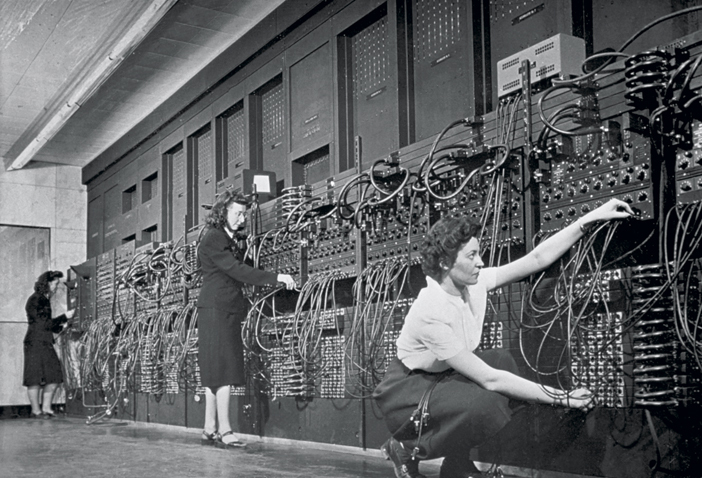
\includegraphics[width=.53\textwidth]{background/pix/rewiring.jpg} \\
%   \begin{credit}
%     \textit{ENIAC Programmers, 1946} \href{https://artsandculture.google.com/asset/eniac-programmers-united-states-army-united-states-army/4AFgcMwMqg1mRw}{U. S. Army Photo from Army Research Labs Technical Library}
%     % (US government works not subject to copyright.)
%   \end{credit}
%   \captionof{figure}{\protect\citetext{ENIAC, reconfigure by rewiring.}{Jean Jennings (left), Marlyn Wescoff (center), and Ruth Lichterman program the ENIAC, circa 1946. U. S. Army Photo}}
% \end{center}


\begin{fig}[eniac]{\protect\citetext{ENIAC，通过重新接线来重新配置。}{照片中，Jean Jennings（左）、Marlyn Wescoff（中）和 Ruth Lichterman 正在为 ENIAC 编程，约1946年。美国陆军照片。}}  \small
  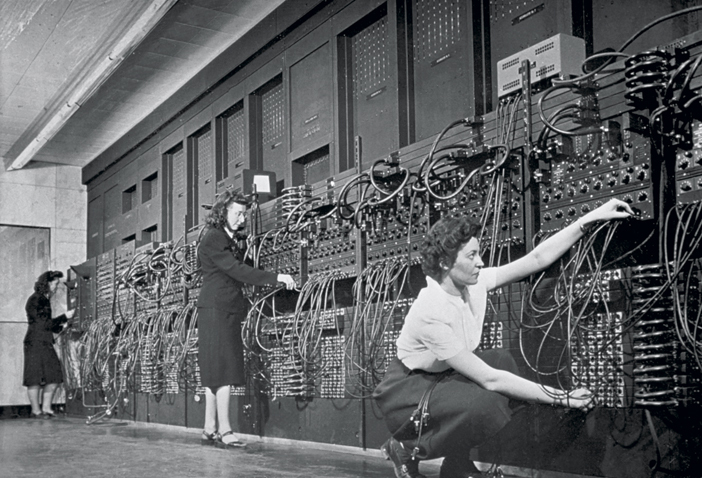
\includegraphics[width=.53\textwidth]{background/pix/rewiring.jpg} \\
  \begin{credit}
    \textit{ENIAC 程序员，1946} \href{https://artsandculture.google.com/asset/eniac-programmers-united-states-army-united-states-army/4AFgcMwMqg1mRw}{U. S. Army Photo from Army Research Labs Technical Library}
    % (US government works not subject to copyright.)
  \end{credit}
\end{fig}


\noindent 想象一下，你有一部手机，当你想从运行浏览器切换到接电话时，
必须拔下一块芯片并换上另一块。\index{hardware}
图中的接线方式比起电烙铁来已经是一种改进，但这还不是最终的答案。
% We want our machines to have their behavior changed by software, not hardware.

\subsection{通用 Turing 机}\index{Universal Turing machine|(}\index{Turing machine!universal|(}
\citetext{技术发展的一个规律是，硬件完成的工作会迁移到软件中}{%
  有一个故事可以说明这种迁移是多么自然，它涉及英国数学家 C~Babbage（查尔斯·巴贝奇）和他的门生 A~Lovelace（阿达·洛夫莱斯）。
  1812年，Babbage 正在编制对数表。
  这些表是由“computers”计算的\Dash 这个词在当时指的是手工进行这些计算的人。\index{computer!person}
  为了检查准确性，他让两个人计算同一张表，然后进行比对。
  他对大量出现的计算结果不一致感到恼火，
  于是萌生了制造一台机器来进行计算的想法。
  他获得了一笔政府拨款，用以设计和建造一台名为“差分机”的机器，
  并于1822年开始建造。
  这是一台单一用途的设备，也就是我们今天所说的计算器。
  当时有一位对他的计算工作产生兴趣的人，是他的熟人 Lovelace（当时她姓 Byron，因为她是诗人 Byron 勋爵的女儿）。
  \protect

\begin{center}
  \protect\small
  \protect\begin{tabular}[t]{c}
  \protect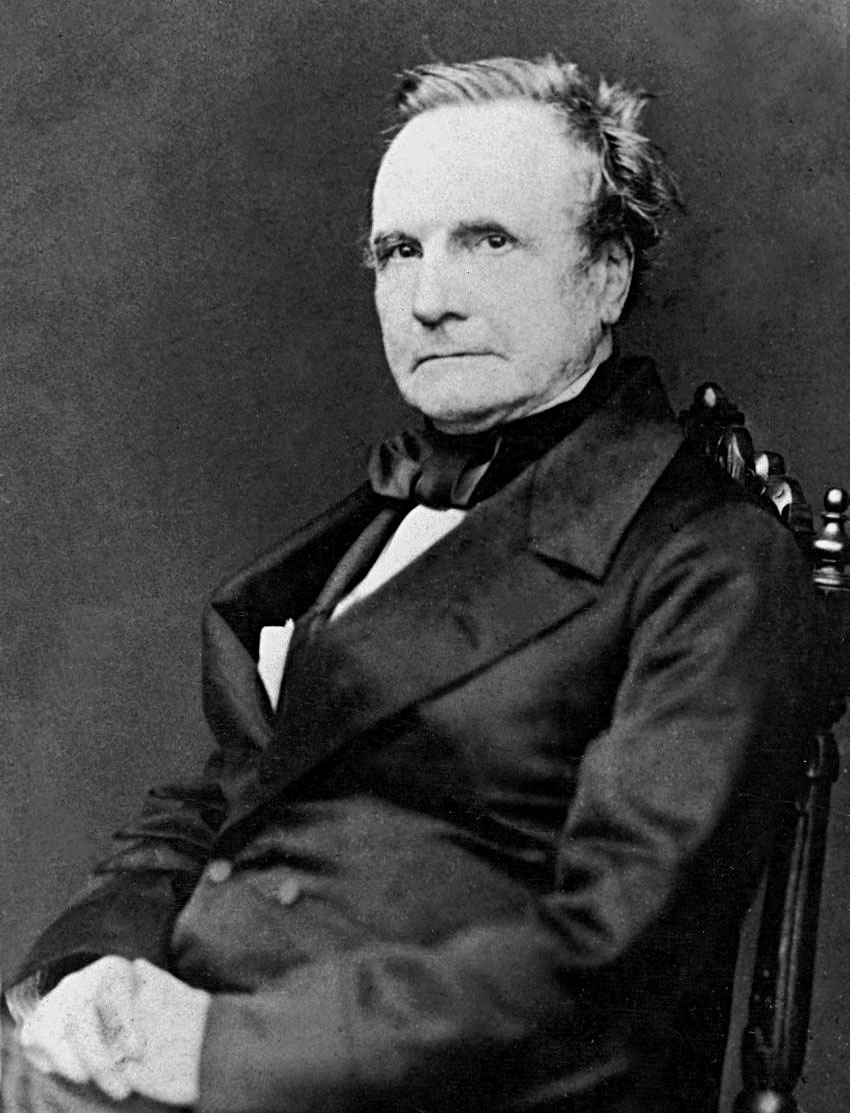
\includegraphics[height=1in]{background/pix/babbage.jpg} \\
  \protect\label{fig:babbage}\protect\href{https://en.wikipedia.org/wiki/Charles_Babbage}{Charles Babbage（查尔斯·巴贝奇），1791--1871} % wikipedia
  \protect\end{tabular}
  \protect\hspace{3em}
  \protect\begin{tabular}[t]{c}
  \protect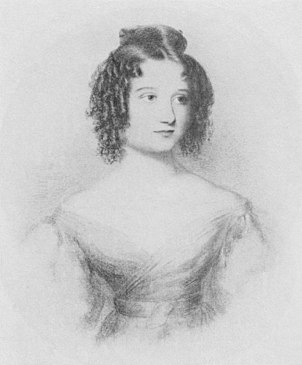
\includegraphics[height=1in]{background/pix/adabyron.jpg} \\
  \protect\label{fig:adabyron}\protect\href{https://en.wikipedia.org/wiki/Ada_Lovelace}{Ada Lovelace（阿达·洛夫莱斯），1815--1852} %
  \protect\end{tabular}
  \protect\end{center}


  然而，这台机器从未完成，因为
  Babbage 又有了制造一台可编程设备的想法，而这诱惑力太大了。\index{programmer!first}
  Lovelace 为一台设想的新机器——分析机——贡献了大量笔记，并因此闻名，被视为第一位程序员。}
典型的例子是编织。\index{weaving}


\begin{center}
  % http://commons.wikimedia.org/wiki/File:Loomwork.jpg
  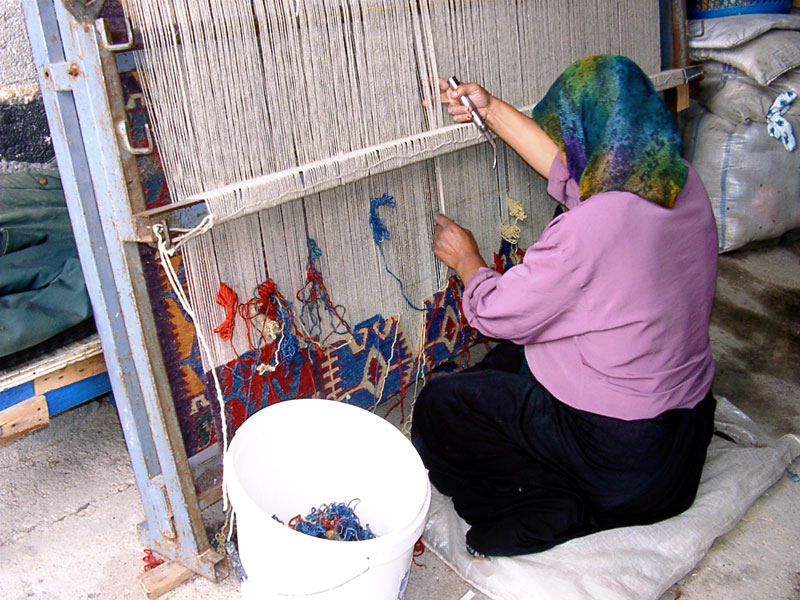
\includegraphics[width=.33\textwidth]{background/pix/loom.jpg}
  \hspace*{2em}
  % http://commons.wikimedia.org/wiki/File:Deutsches_Technikmuseum_Berlin_February_2008_0013.JPG
  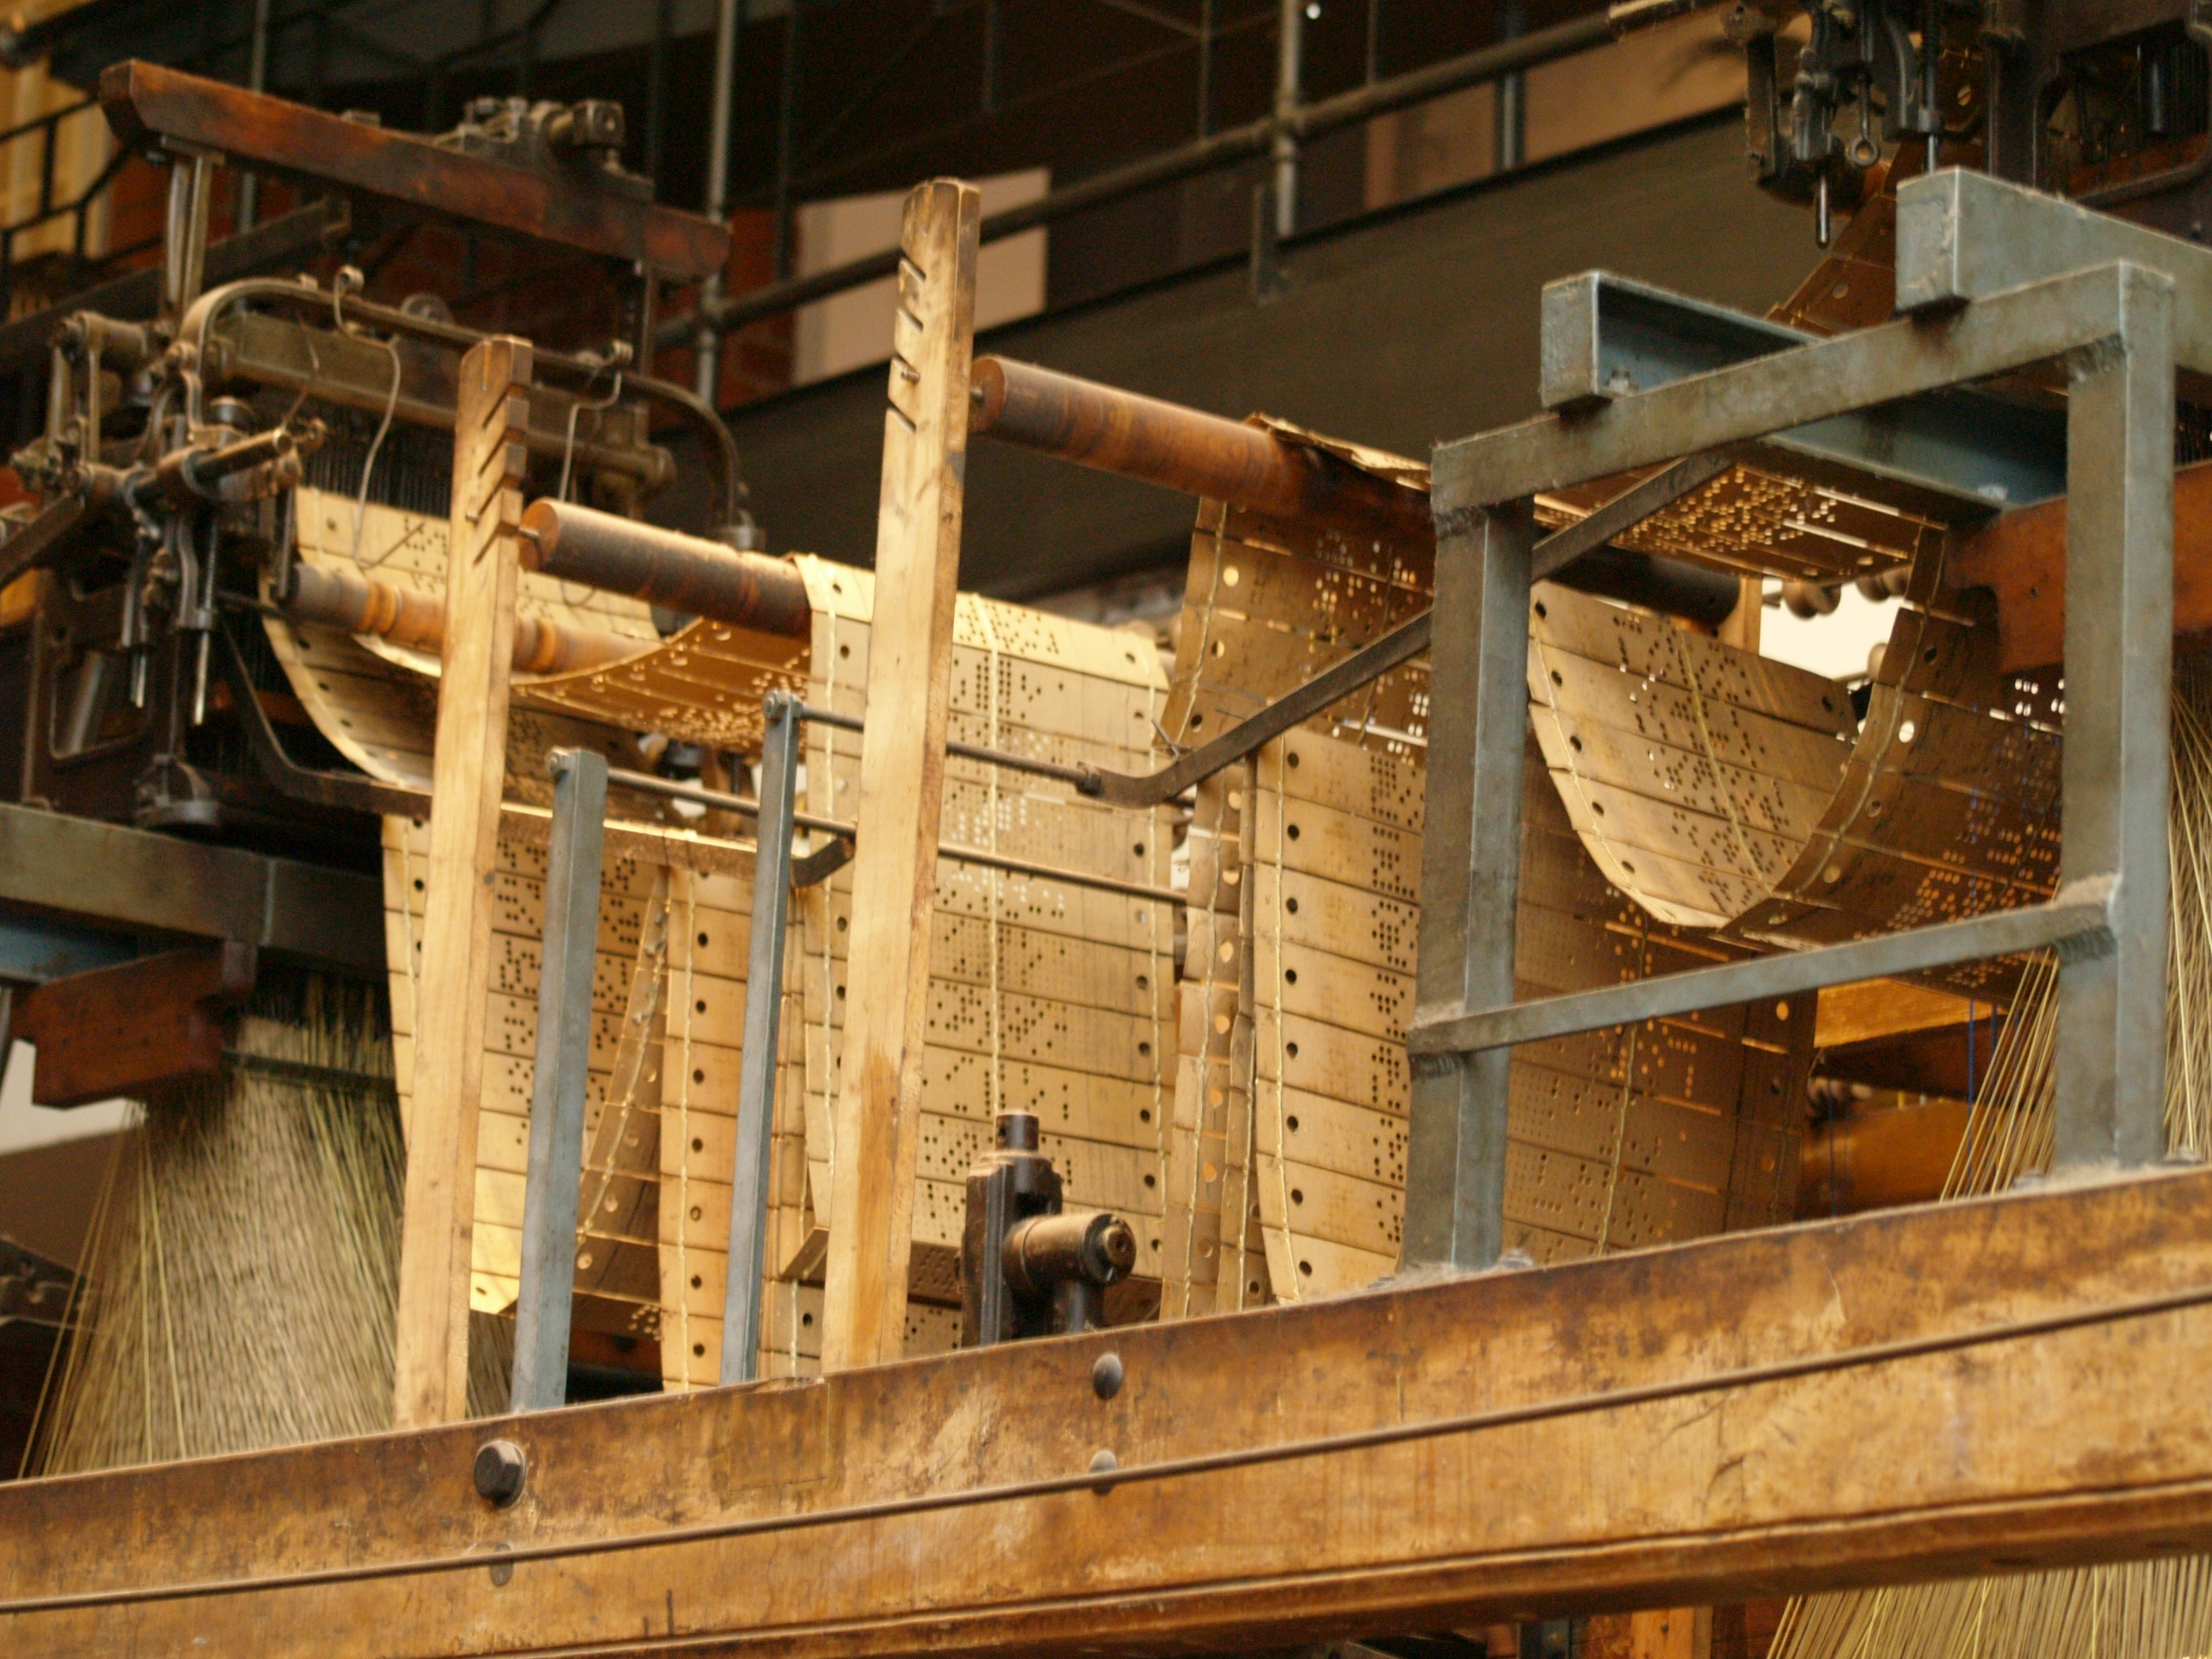
\includegraphics[width=.33\textwidth]{background/pix/jaquardpunchedcards.jpg}
\end{center}


手工织布，如左侧那位织机操作员正在做的，既复杂又缓慢。
我们可以造一台机器来复制她的图案。
但如果我们想要一个不同的图案呢？是否需要另一台机器？
1801年，
\href{https://en.wikipedia.org/wiki/Jacquard_weaving}{J~Jacquard（约瑟夫·玛丽·雅卡尔）}
制造了如右图所示的织布机，\citetext{由卡片控制}{%
  它通过钩子进行编织，钩子提起或放下的位置由卡片上的孔洞决定}。
要获得不同的图案并不需要一台新的织布机，只需要更换一套卡片组即可。

%<*discussion:UniversalTM>
Turing 为计算机引入了与此类似的机制。\index{Turing, Alan}
他构造了一台 Turing 机~$\UTM$，可以向它输入一条纸带，该纸带包含对某台 Turing 机~$\mathcal{M}$ 的描述以及该机器的输入。
然后，$\UTM$ 将表现出与 $\mathcal{M}$ 相同的输入-输出行为。
如果~$\mathcal{M}$
在该输入上停机，那么 $\UTM$ 也将停机并给出相同的输出；
而如果 $\mathcal{M}$ 在该输入上不停机，
那么 $\UTM$ 也不会停机。

只需这一台单独的机器，就能让它表现出任何想要的可计算行为。
因此，我们不需要无穷多台不同的机器，只用 $\UTM$ 就够了。
% This was what we meant by
% saying that a good first take on Turing machines is that they
% are more like a modern computer program than a modern computer\Dash
% on a modern computer, to change behavior we don't change
% the hardware.
%</discussion:UniversalTM>

\margingraphic[l]{0.2\textwidth}{background/pix/snake.png}{\label{fig:ouroboros}\href{https://commons.wikimedia.org/w/index.php?curid=36915535}{衔尾蛇，一条吞食自己尾巴的蛇}}\index{ouroboros}
在陈述 Turing 定理之前，我们先来回答一个经常被问到的问题。
机器~$\UTM$ 似乎引出了一个鸡与蛋的问题：~我们怎么能把一台 Turing 机作为输入给另一台 Turing 机呢？
特别是，既然 $\UTM$ 本身也是一台 Turing 机，
该定理似乎允许将它自身作为输入提供给它自身\Dash 将一台机器喂给它自己，会不会导致无限回归？

\label{page:RepresentingTM}
我们运行 Turing 机，是在纸带上装载好符号，然后按下 \texttt{Start}。
所以我们并不是把机器喂给机器；我们喂给它们的是符号，即事物的表示。
确实，我们可以喂给 $\UTM$ 一个关于它自身的描述，比如一对数 $e,x$，
其中~$e$ 是 $\UTM$ 的索引号（因此在计算上等价于那台机器的源代码），而 $x$ 是输入。
即便如此，宇宙也不会崩溃\Dash
我们完全可以用文本编辑器编辑它自己的源代码，或者让编译器生成它自己的可执行文件。
同理，我们也可以把 $\UTM$ 自己的索引号喂给它。
这样做会引发许多有趣的事情，但首先可以肯定，不存在内在的不可能性。

%<*th:UniversalTM>


\begin{theorem}[Turing, 1936] \label{th:UTM}
存在一台 Turing 机，当输入 $e$ 和 $x$ 时，其输出行为与 $\TM_e$ 在输入 $x$ 上的行为\citetext{相同}{%
  一个技术细节：Turing 机有纸带字母表。
  所以一台通用机的输入或输出只能涉及它被定义为可使用的符号。
  如果另一台机器有不同的纸带字母表，那么通用机该如何模拟它呢？
  和通常一样，我们通过设定让通用机处理另一台机器字母表的表示。
  这类似于日常计算机用二进制来表示十进制数。}。
\end{theorem}


%</th:UniversalTM>

\margingraphicnomag*{0.2\textwidth}{\asydir hp/hp14.pdf}
这就是一台\definend{通用 Turing 机}。\footnote{%
  我们也可以定义一台通用 Turing 机，让它接受单个数 $\cantor(e,x)$ 作为输入。}
\index{Universal Turing machine}\index{Turing machine!universal}%
% We denote such a machine with~$\UTM$.
% Universal machines
% change hardware behavior in software.
% \citetext{This is what a computer's operating
% system does}{%
% }.
此图\footnote{%
  这是一张
\ifbool{MakingPaperCopy}{%
  流程图
}{%
  \citetext{流程图}{%
    流程图被广泛用于勾勒算法；这里有一张来自 XKCD 的图。
    \protect

\begin{center}
    \protect\small
    \protect\begin{tabular}{c}
      \protect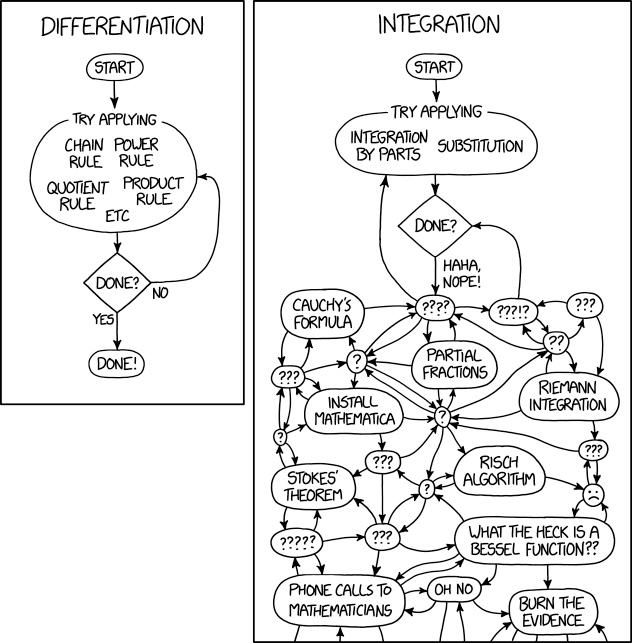
\includegraphics[width=0.25\textwidth]{background/pix/xkcdcalc.png} \\
      \protect\label{fig:xkcdcalc}\protect\href{https://xkcd.com/2117/}{Courtesy xkcd} % wikipedia
    \protect\end{tabular}
    \protect\end{center}

（另参见~\protect\url{http://archive.computerhistory.org/resources/text/Remington_Rand/Univac.Flowmatic.1957.102646140.pdf}）。},
}
  它给出了一个例程的高层示意图。
  我们使用了三种方框。
  圆角方框用于 \protect\texttt{Start} 和
  \protect\texttt{End}。
  矩形方框用于普通的数据操作。
  在后面的图表中我们还会看到菱形方框，
  用于决策，即 \protect\texttt{if} 语句。}\index{flow chart}
勾勒了这样一台机器的行为。

在论证通用机存在之前，我们首先注意到，
通用机器在日常计算中其实很常见。
一方面，
我们可以将此流程图与计算机操作系统的行为进行对比。
操作系统接收一个要运行的程序以及要输入给该程序的数据。
我们可以将程序视作 $\TM_e$，
而将数据视作可解释为数字~$x$ 的比特串。
% The operating system's job is to load the program and feed it the input.
%
操作系统会安排底层硬件表现得如同处理输入~$x$ 的机器~$e$ 一样。
简而言之，与操作系统类似，通用 Turing 机
通过软件改变其行为，
而无需重新插接线。

另一种类似于通用机器的日常计算体验是语言解释器。
下面是与 Racket 解释器的一个交互示例。
在第一个提示符下，我们输入一个例程，它接收
\codeinline!x! 并返回前 \codeinline!x!~个数的和。
在第二个提示符下，我们指定该例程的输入为~$x=4$。
\begin{lstlisting}
$ racket
Welcome to Racket v8.2 [cs].
> (define (triangular x)
      (if (= x 0)
          0
          (+ x (triangular (sub1 x)))))
> (triangular 4)
10
\end{lstlisting}  % $
\label{page:UTM}

计算系统作为通用机器的最直接例子，
是编程语言中的 \codeinline!eval! 语句。\index{eval statement@\texttt{eval} statement}
在下面的第一个提示符下，我们定义了一个例程，它
\citetext{让解释器对输入的表达式求值}{%
  编写一个允许普通用户
  执行任意代码的程序，
  虽然功能强大但并不安全，
  尤其是当这些用户只是从互联网上随意访问时。
  限制用户可以执行的命令，
  即所谓的沙箱化，是谨慎运用这种能力的一部分。
  然而，对我们而言，这些软件工程问题并不相关。}。
在下一个提示符下，我们定义了一个列表（加了引号以防止被求值）。
列表
\codeinline!lambda (i) ...! 描述了一个单输入函数。\footnote{%
  它用“lambda”开始一个函数的定义，因为
  这是 Church 所使用的写法。}
% (in contrast to the definitions
% of the functions \codeinline!triangular! and \codeinline!utm!,
% this function does not have a name and so the definition syntax is
% different).
在第三和第四个提示符下，
解释器对列表中描述的例程求值，
并将其应用于数字~$5$ 和~$0$。
也就是说，就像织布机的打孔卡片一样，
我们可以通过向 \codeinline!utm! 提供任意所需例程的描述，
来改变其行为。
\begin{lstlisting}
> (define (utm s)
      (eval s))
> (define test '(lambda (i) (if (= i 0) 1 0)))
> ((utm test) 5)
0
> ((utm test) 0)
1
\end{lstlisting}

最后，关于该定理的证明，
证明某物存在的最简单方法就是将其构造出来。
我们已经展示过一个本质上就是通用 Turing 机的实例。
在第一章末尾的第~\pageref{extra:TuringMachineSimilator} 页，
我们使用过一个 Turing 机模拟器程序，它
从文件中读取 Turing 机的描述，
然后运行它。
该代码是用 Racket 写的，但
Church 论题断言，我们同样可以写出一台
具有相同行为的 Turing 机。
% (For a Universal Turing machine that meets the criteria, we must not input
% the arbitrary Turing machine from a file, but instead we
% input its index, which we then convert to a Turing machine.
% But we've already argued that we can write a routine to go from
% the index to the Turing machine.)
\index{Universal Turing machine|)}\index{Turing machine!universal|)}

\subsection{一致性}\index{uniformity|(}
考虑这样一个任务：给定一个实数 $r\in\R$，
编写一个程序来输出它的各位数字。
更准确地说，构造一台 Turing 机 $\TM_r$，
使得当输入 $n\in\N$ 时，$\TM_r$ 输出
\citetext{$r$ 的第 $n$ 位小数}{%
  如果数字 $r$ 有不止一种表示法，那么我们可以，
  比如说，输出以 $0$ 结尾的那一种。}
（当~$n=0$ 时，
它输出小数点左边的整数部分）。

我们知道，
并非对所有~$r$ 都能做到这一点，因为虽然
存在不可数多个实数，但 Turing 机只有可数多个。
但究竟是什么阻碍了我们呢？
编程的乐趣之一就在于感觉能让机器做任何事\Dash
为什么不能编写一个程序来输出我们想要的任何数字呢？

确实存在一些实数，可以为它们编写这样的程序，
比如~$11.25$。
\begin{lstlisting}
(define (one-quarter-decimal-places n)
  (cond
      [(= n 0) 11]
      [(= n 1) 2]
      [(= n 2) 5]
      [else 0]))
\end{lstlisting}
对于一个更一般的数，比方说 $r=0.703\ldots$\,，
我们可能会一时想到用穷举法来处理它。
\begin{lstlisting}
(define (r-decimal-place n)
  (cond
    [(= n 0) 0]
    [(= n 1) 7]
    [(= n 2) 0]
    [(= n 3) 3]
    ...
  ))
\end{lstlisting}
但这很可笑。
程序长度有限，因此
不可能包含无限多个分支。

也就是说，由于 \codeinline!if! 语句，
如下程序在输入~$n=7$ 时的行为，
与它在其他输入上的行为互不相关。
\begin{lstlisting}
(define (foo n)
  (if (= n 7)
      42
      (* 2 n)))
\end{lstlisting}
但一个程序只能包含有限多个这样
行为不同的分支。
Turing 机仅有有限条指令这一事实，
对其行为施加了一致性条件。

\begin{example} \label{ex:NineInPi}
以这种方式将“某物可计算”与“它是一致可计算的”这两个观念联系起来，会产生一些令人惊讶的后果。
考虑这样一个问题：编写一个程序，它接收一个数~$n$ 作为输入，然后
判定在 $\pi=3.14159\ldots$ 的十进制展开中，是否
存在 $n$ 个
\citetext{连续的 $9$}{%
  在第 $762$ 位小数处，连续出现了六个 $9$。
  这被称为 Feynman（费曼）点；参见
  \protect\url{https://en.wikipedia.org/wiki/Feynman_point}。
  大多数专家猜想，对于任何~$n$，$\pi$ 的十进制
  展开中都包含连续 $n$ 个 $9$ 的序列，但至今既无人证明也无人推翻这一点。}。

这有两种可能。
要么对于所有~$n$，这样的序列都存在；要么存在某个 $N$，
使得当长度小于~$N$ 时存在连续的 $9$ 序列，
而当 $n\geq N$ 时不存在这样的序列。
因此，这个问题实际上已经解决：以下两个程序之一就是正确的程序
（为说明起见，此处取 $N=1234$）。\label{disc:HP}
\begin{center}
\vspace*{-4ex}
\begin{minipage}[t]{0.4\linewidth}%
\begin{lstlisting}
(define (sequence-of-nines-0 n)
  1)
\end{lstlisting}%
\end{minipage}%
\hspace*{2em}
\begin{minipage}[t]{0.4\linewidth}%
\begin{lstlisting}
(define (sequence-of-nines-1 n)
  (if (< n 1234)
      1
      0))
\end{lstlisting}%
\end{minipage}%
\vspace*{-2ex}
\end{center}

这个论证的一个惊人之处在于，这两个例程似乎与 $\pi$ 并没有多大关系。
同样惊人且或许令人不安的是，我们在没有展示具体解法的情况下，就证明了该问题是可解的。
也就是说，
\citetext{“证明这个函数是可计算的”与“拥有计算它的算法”是两回事}{%
  这有点类似于
  Schr\"odinger（薛定谔）的猫悖论
  (参见 \protect\url{https://en.wikipedia.org/wiki/Schr\%C3\%B6dinger's_cat})，
  因为看起来两者中总有一个是对的，
  但我们就是不知道是哪一个。
  }
\begin{equation*}
  f(n)=
  \begin{cases}
    1 &\case{if $\pi$ has $n$ consecutive nines}  \\
    0 &\case{otherwise}
  \end{cases}
\end{equation*}
这表明，
\citetext{“如果你能为某个东西编写程序，那它就是可计算的”这种说法}{引自 \autocite{SE:JohnL}：
  “我相信大多数人第一次遇到这种证明/结论时，都会感到有些困惑。
  % Or at least myself.
  % The essential point is
  % we do not have to identify/construct/bind to one
  % algorithm that decides [it].
  \ldots{}
  我们并不需要完全理解[那个问题]是什么。
  我们只需要知道，存在一个算法能够判定[它]，无论[答案]最终是什么。
  这偏离了……你可能在接触计算理论之前就有的……那种朴素的可判定性观念。”}
作为一种初步理解或许有用，但至少
遗漏了一些重要的微妙之处。

相比之下，假设我们有一个例程 \codeinline{pi_decimals}
它接收输入~$i\in\N$ 并输出
\citetext{$\pi$ 的第 $i$ 位小数}{%
  如前所述，有些实数有两种十进制
  表示，一种以 $0$ 结尾，一种以 $9$ 结尾。
  但所有这样的数都是有理数（正如“以 $0$ 结尾”所暗示的），
  而 $\pi$ 不是有理数，所以 $\pi$ 不属于这类数。}。
利用它，我们可以编写一个程序，接收输入~$n$，然后
遍历 $\pi$ 的各位数字，
查找连续的 $n$ 个 $9$。
这种方法的好处是，它不仅给出了答案是否存在的结论，还实际构造出了答案。
这种方法也具有“一致性”，因为我们可以
修改它以使用其他例程（如 \codeinline{e_decimals}），
从而在其他数字中寻找连续的 $9$ 串。
然而，这种方法也有一个缺点：如果存在某个 $N$，
使得对于 $n\geq N$，$\pi$ 的十进制展开中都不存在连续 $n$ 个 $9$，
那么这个程序将
无休止地搜索下去，永远无法发现这一情况。
\end{example}


\index{uniformity|)}

\subsection{参数化}\index{parametrization|(}
通用性意味着，存在一台 Turing 机，它
接收输入 $e$ 和~$x$，并返回与在输入~$x$ 上运行 $\TM_e$ 所得相同的值，
包括当 $\TM_e$ 在该输入上不停机时，它也不停机。
也就是说，存在一个可计算
函数 $\map{\phi}{\N^2}{\N}$，使得
若 $\TMfcn_e(x)\converges$ 则 $\phi(e,x)=\TMfcn_e(x)$，若 $\TMfcn_e(x)\diverges$ 则 $\phi(e,x)\diverges$。

在这里，参数~$e$ 从函数的自变量转变为索引，
从而使得 $\phi(e,x)$ 变成了 $\TMfcn_e(x)$。
我们现在将其推广。
从一个接收两个输入的程序开始，
例如下面这个。
\begin{lstlisting}
(define (P x y)
  (+ x y))
\end{lstlisting}
冻结第一个自变量，
结果得到一个单输入程序。
这里，我们先将 $x$ 冻结为~$7$，然后冻结为 $8$。


\begin{center}
\vspace*{-4ex}
\begin{minipage}[t]{0.4\linewidth}%
\begin{lstlisting}
(define (P_7 y)
  (P 7 y))
\end{lstlisting}
\end{minipage}%
\hspace*{2em}
\begin{minipage}[t]{0.4\linewidth}%
\begin{lstlisting}
(define (P_8 y)
  (P 8 y))
\end{lstlisting}
\end{minipage}%
\vspace*{-2ex}
\end{center}

这称为\citetext{\definend{部分应用（partial application）}}{%
  参见 \autocite{wiki:PartialApplication}。}，
因为我们没有冻结所有的输入变量。
相反，我们对
\citetext{\definend{变量~$x$ 进行参数化}}{%
  参数（parameter）是在同一种形式的方程中变化的常数。
  例如，研究二次函数的人可能会考虑方程族 $y=ax^2$；这里 $a$ 就是一个参数。
  所以参数是一种固定的变量。
  （令人难忘的是 A~Perlis 的一句警句，
  “一个人的常量是另一个人的变量。”
  \autocite{Perlis}）
}\index{parametrizing}\index{parameter}
，从而得到一族程序
\codeinline!P_0!、\codeinline!P_1! 等等。

显然，这一族程序与起始程序是相关的。
记上述起始程序~\codeinline{P} 所计算的函数为 $\psi(x,y)=x+y$，
部分应用便给出了如下的函数族：
$\psi_0(y)=y$、$\psi_1(y)=1+y$、$\psi_2(y)=2+y$、\ldots\sentencespace
一般而言，下面的结果表明，
从一个起始 Turing 机（或可计算函数）的索引以及被冻结的值，
我们可以计算出这一族成员的索引。

%<*th:smn>


\begin{theorem}[\smn{} 定理，或称参数定理] \label{th:smn}
\index{Parameter theorem}\index{s-m-n theorem@$s$-$m$-$n$ theorem}
对任意 $m,n\in\N$，存在一个可计算的全函数 $\map{s_{m,n}}{\N^{1+m}}{\N}$
使得对任意 $m+n$ 元函数
$\TMfcn_e(x_0,\ldots\, x_{m-1},x_m,\ldots\, x_{m+n-1})$，
将前 $m$ 个变量冻结于 $a_0,\ldots\, a_{m-1}\in\N$
便得到 $n$ 元可计算函数
$\TMfcn_{s(e,a_0,\ldots a_{m-1})}(x_m,\ldots\, x_{m+n-1})$。% \footnotemark[1]
\end{theorem}


% \footnotetext[1]{%
%   This result is stated in terms of functions, not machines, because
%   the machines need not be the same.
%   That is, they may be unequal as sets of four-tuples.
%   But they will have the same input-output behavior, which means
%   the same function.}
%</th:smn>
% The function $\TMfcn_e(x_0,\ldots x_{m-1},x_m,\ldots x_{m+n-1})$ could be
% partial, that is, it could be that the Turing machine
% $\TM_e$ fails to halt on some inputs $x_0,\ldots x_{m-1},x_m,\ldots x_{m+n-1}$.

\begin{proof}
%<*pf:smni>
我们将构造函数~$s$ 来满足三个
要求：~\citetext{它必须是有效的}{%
  事实上，仔细分析表明它是原始递归的。}；
它必须以索引~$e$ 和一个 $m$ 元组 $a_0,\ldots\, a_{m-1}$ 作为输入；
并且它必须输出一台机器~$\hat{\TM}$ 的索引，使得该机器
在给定输入 $x_m,\ldots\, x_{m+n-1}$ 时，
将返回值 $\TMfcn_e(a_0,\ldots\, a_{m-1},x_m,\ldots\, x_{m+n-1})$，
若该函数发散则不停机。

其思想是：计算~$s$ 的机器将构建~$\hat{\TM}$ 的指令集。
我们能从指令集有效地得出索引，由此即可完成证明。
%</pf:smni>

%<*pf:smnii>
下方左侧是计算函数~$s$ 的机器的流程图。
在其第三个方框中，它生成了右侧简图所示的四元组指令集
$\hat{\TM}$。
左边的机器需要 $a_0,\ldots\, a_{m-1}$ 用于
右侧流程图的第二、三、四框，
还需要 $e$ 用于 $\hat{\TM}$ 的第五框。
%</pf:smnii>
（我们通常尽量避免纠缠于 Turing 机输入输出表示的细节，
但为了尽可能清晰，在右侧的流程图中，我们假设其输入为一元表示，
输入之间用空白符分隔，且机器启动时读写头位于输入最左边的
\str{1} 下方。）
%<*pf:smniii>
\begin{center}
  \vcenteredhbox{\includegraphics{\asydir flowcharts/flowcharts00.pdf}}
  \hspace{3em}
  \vcenteredhbox{\includegraphics{\asydir flowcharts/flowcharts01.pdf}}
\end{center}

最后，注意左边的例程并不运行右边的例程。
相反，它返回实现右侧流程图的 Turing 机 $\hat{\TM}$ 的索引。
它可以在不知道右侧例程是否会停机的情况下生成右侧流程图的源代码，
并由此源代码计算出索引。
因此，由左侧流程图计算的函数~$s$ 是全函数。
%</pf:smniii>
\end{proof}

在记号 $s_{m,n}$ 中，
下标~$m$ 是被冻结的输入个数，
而下标~$n$ 是剩余的自由输入个数。
这些下标可能略显繁琐，我们通常省略它们。

\smn{} 定理的关键点在于它给出的不仅是一个可计算函数，更是一族相关的函数。

\begin{example}
考虑由该流程图描述的双输入例程。
\begin{equation*}
  \vcenteredhbox{\includegraphics{\asydir flowcharts/flowcharts1007.pdf}}
  \tag{$*$}
\end{equation*}
由 Church 论题，存在一台 Turing 机与该草图匹配。
% computing the function $\psi(x,y)=x\cdot y$.
记其索引为~$e_0$。
（下标 ‘0’ 意在强调这个索引是固定的，而非变量；它是某一特定 Turing 机的编号。）

下方左侧是机器 $\TM_{s(e_0,0)}$ 的流程图，它将~$x$ 的值固定为~$0$，从而计算函数 $\TMfcn_{s(e_0,0)}(y)=0$。
例如，$\TMfcn_{s(e_0,0)}(5)=0$。
类似地，另外两个是概括 $\TM_{s(e_0,1)}$ 和~$\TM_{s(e_0,2)}$ 的流程图，
% freezing the value of $x$ at $1$ and~$2$ and therefore
它们计算函数 $\TMfcn_{s(e_0,1)}(y)=y$ 和 $\TMfcn_{s(e_0,2)}(y)=2y$。
\begin{center}
  \vcenteredhbox{\includegraphics{\asydir flowcharts/flowcharts1008.pdf}}
  \hspace{2em}
  \vcenteredhbox{\includegraphics{\asydir flowcharts/flowcharts1009.pdf}}
  \hspace{2em}
  \vcenteredhbox{\includegraphics{\asydir flowcharts/flowcharts1010.pdf}}
  \hspace{2em}\ldots
\end{center}
以下是一般的家族成员，$\TM_{s(e_0,x)}$。
\begin{equation*}
  \vcenteredhbox{\includegraphics{\asydir flowcharts/flowcharts1011.pdf}}
  \tag{$**$}
\end{equation*}
将 ($**$) 与~($*$) 对比。
不同之处在于，($**$) 中的机器并不读入~$x$；相反，若将它们视为程序而非 Turing 机，则 $x$ 被硬编码在源代码的体部中。
\end{example}

该示例展示了 \smn{} 定理如何使我们从单个可计算函数 $\TMfcn_{e_0}$ 得到函数序列
$\TMfcn_{s(e_0,x)}$。
这是一个相关的函数族，
\citetext{它是由~$x$ 参数化的}{%
  如果我们从一个双输入函数
  $\map{\TMfcn_{e_0}(x,y)}{\N^2}{\N}$ 开始，那么对于每个~$x$，\smn{}
  定理实际上产生了一个单输入函数 $\map{\TMfcn_{s(e_0,x)}}{\N}{\N}$。
  也就是说，将 $\N$、$\N$ 和 $\N$ 分别替换为 $A$、$B$ 和 $C$，
  它就把从 $A\times B$ 到~$C$ 的二元映射集合，变换为从 $A$ 到~$D$ 的映射集合中的一个成员，其中 $D$
  是从 $B$ 到~$C$ 的映射集合。
  在某些语境下，例如函数式编程中，这被称为
  \definend{柯里化（currying）}.\index{currying}
}，因为 $e_0$ 是固定的。

换句话说，这个函数族是一致可计算的\Dash 那个单一的可计算函数~$s$（更精确地说是 $s_{1,1}$）从索引~$e_0$ 和参数值~$x$ 出发，映射到 ($**$) 中结果的索引。
所以 \smn{} 定理是关于一致性的。
\index{parametrization|)}

% ..............................................................
\begin{exercises}
\recommended


\begin{exercise}
\begin{credit}
  始于\href{https://cs.stackexchange.com/questions/69197/difference-between-turing-machine-and-universal-turing-machine}{Stack Exchange}
\end{credit}
你的学习小组里有人问：
“通用 Turing 机能做哪些普通 Turing 机做不到的事？”
帮他们理解一下。
\begin{answer}\verified
  通用 Turing 机本身也是一台普通的 Turing 机，因为它只是列表 $\TM_0$、$\TM_1$、\ldots\sentencespace 中的另一台而已。
  或许你的朋友想问的是：“通用 Turing 机能做哪些非通用的 Turing 机做不了的事？”
  每台 Turing 机都执行一项任务。
  有些机器接受单个输入然后将其翻倍，
  有些则将其输入解释为两个数字然后相加。
  通用 Turing 机期待两个输入，$e$ 和~$x$，
  而它的输出与机器 $\TM_e$ 在输入~$x$ 上的输出相同，
  若那台机器不停机，它也不停机。
  它的通用性在于，任何能被机械地产生的输入-输出行为，都可以由这一台设备产生。
\end{answer}
\end{exercise}

\begin{exercise}
是否有人曾建造出通用 Turing 机，
或与之等效的设备？抑或它仅仅停留在理论层面？
\begin{answer}\verified
  每一台通用计算机，包括任何标准的笔记本电脑或手机，
  本质上都是一台通用 Turing 机。

  \textit{注：}
  有些观察者反对“通用计算机本质上是 Turing 机”这一论断，
  理由是笔记本电脑并不具有无限多的内存。
  确实如此。
  但同样不可否认的是，这样的机器可以连接到外部存储器——
  也许是云存储，也许是允许它在纸带上做标记的设备——
  从而它并不受限于内置的 RAM。

  有人还会继续反驳说，物理宇宙中只有数量有限的基本粒子可以用来构成比特，
  因此内存终究不是无限的。
  这或许是真的\Dash 它似乎与当前的物理学相符，
  尽管我们也可以回击说，在大爆炸演变为大挤压（或未来无论发生什么）之前，
  我们根本没有足够的时间去耗尽现有的所有比特。

  然而，在关于 Church 论题的章节中我们曾指出，
  Turing 机的定义将直观上的可计算概念精确化了。
  也就是说，“Turing 机”的关键在于，
  它是思考算法的正确模型；它是一种数学理想化。
  笔记本电脑则是同一概念的物理实例化。

  确实，从某种意义上说它们不能是同一事物，因为那将是类型错误\Dash
  一个的类型是“数学对象”，而另一个的类型是“物理对象”。
  同理，木工用的丁字尺是直角这一数学理想的实例化。
  以无人能制造出精确到小数位数超过宇宙中基本粒子数的完美直角为由，
  断言丁字尺是不合法的，这似乎忘记了我们为何觉得思考模型是有用的。
  实例化的本质即是理想化。
\end{answer}
\end{exercise}

\begin{exercise}
一台通用 Turing 机能够模拟另一台通用 Turing 机吗？
甚至，它能模拟它自己吗？
\begin{answer}\verified
  能。
  如果 $\TM_{e_0}$ 和 $\TM_{e_1}$ 是通用 Turing 机，
  那么给第一台输入 $e_1$ 和 $x$，
  将产生与第二台完全相同的输入输出行为。
  同样地，给 $\TM_{e_0}$ 输入 $e_0$ 和 $x$，
  其行为将与它自身完全一致。
\end{answer}
\end{exercise}

\recommended

\begin{exercise}
\begin{credit}
  来自
  \href{https://cs.stackexchange.com/q/41854/67754}{Stack Exchange 上的一个问题}.
\end{credit}
你们班上有同学说：
“我搞不懂通用 Turing 机。
一台机器怎么能模拟拥有更多状态的另一台机器呢？”
请纠正他们的错误认识。
\begin{answer}\verified
  通用机并不是使用自己的状态去模拟另一台机器的状态。
  相反，它拥有这些状态的编码，并对这些编码进行操作。
  简而言之，它通过软件进行模拟，因此通用机自身的状态数量与此无关。
\end{answer}
\end{exercise}

\begin{exercise}
是否存在不止一台通用 Turing 机？
\begin{answer}\verified
是的，根据~\zcref{lem:EveryCompFcnHasInfManyIndices}，
每个可计算函数都有无穷多个索引。
因此，如果 $\TM_e$ 是通用的，那么其关联函数~$\TMfcn_e$
就有无穷多个互不相同的索引：
$\TMfcn_e=\TMfcn_{e_0}=\TMfcn_{e_1}=\cdots\,$。
这些机器
$\TM_{e_0}$, $\TM_{e_1}$, \ldots{} 各不相同，但它们具有相同的
输入输出行为，因此都是通用的。
\end{answer}
\end{exercise}

% \begin{exercise}
% What happens if we feed a Universal Turing machine to itself?
% For instance, where the index~$e_0$ is such that
% $\TMfcn_{e_0}(e,x)=\TMfcn_e(x)$ for all~$x$,
% what is the value of
% $\TMfcn_{e_0}(e_0,5)$?
% \begin{answer}
% We know that $5$ equals $\cantor(2,0)$, that is, $\pair(5)=\sequence{2,0}$.
% So in $\TMfcn_{e_0}(e_0,5)$ the argument to $\TMfcn_{e_0}$ is the
% value of $\TMfcn_2(0)$.
% So, where $\pair(\TMfcn_2(0))=\sequence{a,b}$, the value of
% $\TMfcn_{e_0}(e_0,5)$ is $\TMfcn_a(b)$.
% \end{answer}
% \end{exercise}

\recommended

\begin{exercise}
考虑函数 $f(x_0,x_1)=3x_0+x_0\cdot x_1$。
\begin{exparts}
\item 将 $x_0$ 冻结为值~$4$。
  得到的一元函数是什么？
\item 将 $x_0$ 冻结为~$5$。
  得到的一元函数是什么？
\item 将 $x_1$ 冻结为~$0$。
  得到的函数是什么？
\end{exparts}
\begin{answer}\verified
我们将 $x_i$ 冻结为值~$a$ 所得的函数记作 $f_{i,a}$。
\begin{exparts}
\item 得到的一元函数是 $f_{0,4}(x_1)=12+4x_1$。
\item 得到的一元函数是 $f_{0,5}(x_1)=15+5x_1$。
\item 得到的一元函数是 $f_{1,0}(x_0)=3x_0$。
\end{exparts}
\end{answer}
\end{exercise}

\begin{exercise}
考虑
$f(x_0,x_1,x_2)=x_0+2x_1+3x_2$。
\begin{exparts}
\item 将 $x_0$ 冻结为值~$1$。
  得到的二元函数是什么？
\item 将 $x_0$ 冻结为 $2$ 会得到什么二元函数？
\item 设 $a$ 为自然数。
  将 $x_0$ 冻结为 $a$ 会得到什么二元函数？
\item 将 $x_0$ 冻结为~$5$，$x_1$ 冻结为~$3$。
  得到的一元函数是什么？
\item 对于 $a,b\in\N$，将 $x_0$ 冻结为~$a$，$x_1$ 冻结为~$b$ 会得到什么一元函数？
\end{exparts}
\begin{answer}\verified
我们用 $\hat{f}$ 来命名各个函数。
\begin{exparts}
\item 得到的二元函数是
  $\hat{f}(x_1,x_2)=1+2x_1+3x_2$。
\item 结果是二元函数
  $\hat{f}(x_1,x_2)=2+2x_1+3x_2$。
\item 这给出
  $\hat{f}(x_1,x_2)=a+2x_1+3x_2$。
\item 这得到一元函数
  $\hat{f}(x_2)=11+3x_2$。
\item 结果是
  $\hat{f}(x_2)=a+2b+3x_2$。
\end{exparts}
\end{answer}
\end{exercise}

\recommended


\begin{exercise}
假设由该流程图描绘的 Turing 机的索引为~$e_0$。
\begin{center}
  \includegraphics{\asydir flowcharts/flowcharts1000.pdf}
\end{center}
\begin{exparts}
\item 描述函数 $\TMfcn_{s_{1,1}(e_0,1)}$。
\item 求 $\TMfcn_{s_{1,1}(e_0,1)}(0)$、
  $\TMfcn_{s_{1,1}(e_0,1)}(1)$ 和~$\TMfcn_{s_{1,1}(e_0,1)}(2)$ 的值。
\item 描述函数 $\TMfcn_{s_{1,1}(e_0,0)}$。
\item 求 $\TMfcn_{s_{1,1}(e_0,0)}(0)$、
  $\TMfcn_{s_{1,1}(e_0,0)}(1)$ 和~$\TMfcn_{s_{1,0}(e_0,0)}(2)$ 的值。
\end{exparts}
\begin{answer}\verified
由机器的流程图，我们得到其关联函数
$\TMfcn_{e_0}(x_0,x_1)=x_0+x_1$。
\begin{exparts}
\item $s_{1,1}$ 的两个下标意味着
  我们将冻结第一个输入，并将第二个保留为变量。
  所以 $\TMfcn_{s_{1,1}(e_0,1)}$ 将是一个一元函数。
  参数 $e_0$ 和~$1$ 表明我们正在处理
  Turing 机~$e_0$（即题目中给出流程图的那台机器），
  且输入被冻结为 $x_0=1$。
  此流程图给出了结果的示意。
  \begin{center}
    \includegraphics{\asydir flowcharts/flowcharts1001.pdf}
  \end{center}
  该函数为 $\TMfcn_{s_{1,1}(e_0,1)}(x_1)=1+x_1$。
\item 其值为 $\TMfcn_{s_{1,1}(e_0,1)}(0)=1$、
  $\TMfcn_{s_{1,1}(e_0,1)}(1)=2$ 和~$\TMfcn_{s_{1,1}(e_0,1)}(2)=3$。
\item 记号 $s_{1,1}(e_0,0)$ 表示我们处理 Turing 机~$e_0$，
  将第一个输入冻结为 $x_0=0$，
  并将第二个输入保留为变量。
  此流程图展示了其大意。
  \begin{center}
    \includegraphics{\asydir flowcharts/flowcharts1002.pdf}
  \end{center}
  该函数为 $\TMfcn_{s_{1,1}(e_0,1)}(x_1)=0+x_1=x_1$。
\item 我们有 $\TMfcn_{s_{1,1}(e_0,0)}(0)=0$、
  $\TMfcn_{s_{1,1}(e_0,0)}(1)=1$ 和~$\TMfcn_{s_{1,1}(e_0,0)}(2)=2$。
\end{exparts}
\end{answer}
\end{exercise}

\begin{exercise}
设由该流程图描绘的 Turing 机的索引为~$e_0$。
\begin{center}
  \includegraphics{\asydir flowcharts/flowcharts1003.pdf}
\end{center}
\begin{exparts}
\item 描述函数 $\TMfcn_{s_{1,2}(e_0,1)}$。
\item 求 $\TMfcn_{s_{1,2}(e_0,1)}(0,1)$、
  $\TMfcn_{s_{1,2}(e_0,1)}(1,0)$ 和~$\TMfcn_{s_{1,2}(e_0,1)}(2,3)$。
\item 描述函数 $\TMfcn_{s_{2,1}(e_0,1,2)}$。
\item 求 $\TMfcn_{s_{2,1}(e_0,1,2)}(0)$、
  $\TMfcn_{s_{2,1}(e_0,1,2)}(1)$ 和~$\TMfcn_{s_{2,1}(e_0,1,2)}(2)$。
\end{exparts}
\begin{answer}\verified
由机器的流程图可知，关联函数为
$\TMfcn_{e_0}(x_0,x_1,x_2)=x_0+x_1\cdot x_2$。
\begin{exparts}
\item 记号 $s_{1,2}(e_0,1)$ 表示
  我们处理 $\TM_{e_0}$，
  将第一个输入冻结为 $x_0=1$，
  并将第二个和第三个输入保留为变量。
  此流程图勾勒了其行为。
  \begin{center}
    \includegraphics{\asydir flowcharts/flowcharts1004.pdf}
  \end{center}
  该函数为 $\TMfcn_{s_{1,2}(e_0,1)}(x_1,x_2)=1+x_1\cdot x_2$。
\item 我们有 $\TMfcn_{s_{1,2}(e_0,1)}(0,1)=1$、
  $\TMfcn_{s_{1,2}(e_0,1)}(1,0)=1$ 和~$\TMfcn_{s_{1,2}(e_0,1)}(2,3)=7$。
\item $s_{2,1}(e_0,1,2)$ 表示我们从 $\TM_{e_0}$ 出发，
  将第一个输入冻结为 $x_0=1$，第二个输入冻结为 $x_1=2$，
  并将第三个输入保留为变量。
  此流程图勾勒了结果。
  \begin{center}
    \includegraphics{\asydir flowcharts/flowcharts1005.pdf}
  \end{center}
  该函数为 $\TMfcn_{s_{2,1}(e_0,1,2)}(x_2)=1+2\cdot x_2$。
\item 其值为 $\TMfcn_{s_{2,1}(e_0,1,2)}(0)=1$、
  $\TMfcn_{s_{2,1}(e_0,1,2)}(1)=3$ 和~$\TMfcn_{s_{2,1}(e_0,1,2)}(2)=5$。
\end{exparts}
\end{answer}
\end{exercise}

\recommended


\begin{exercise}
假设由该流程图描绘的 Turing 机的索引为~$e_0$。
\begin{center}
  \includegraphics{\asydir flowcharts/flowcharts1006.pdf}
\end{center}
\begin{exparts*}
\item 描述 $\TMfcn_{s_{1,1}(e_0,0)}$。
\item 求 $\TMfcn_{s_{1,1}(e_0,0)}(5)$。
\item 描述 $\TMfcn_{s_{1,1}(e_0,1)}$。
\item 求 $\TMfcn_{s_{1,1}(e_0,1)}(5)$。
\item 描述 $\TMfcn_{s_{1,1}(e_0,2)}$。
\item 求 $\TMfcn_{s_{1,1}(e_0,2)}(5)$。
\end{exparts*}
\begin{answer}\verified
由机器的流程图可知，关联函数如下：
\begin{equation*}
  \TMfcn_{e_0}(x_0,x_1)=
  \begin{cases}
    x_1  &\case{if $x_0\leq 1$}  \\
    \,\diverges &\case{otherwise}
  \end{cases}
\end{equation*}
\begin{exparts}
\item $\TMfcn_{s_{1,1}(e_0,0)}(x_1)=x_1$
\item $\TMfcn_{s_{1,1}(e_0,0)}(5)=5$
\item $\TMfcn_{s_{1,1}(e_0,1)}(x_1)=x_1$
\item $\TMfcn_{s_{1,1}(e_0,1)}(5)=5$
\item $\TMfcn_{s_{1,1}(e_0,2)}(x_1)\diverges$
\item $\TMfcn_{s_{1,1}(e_0,2)}(5)\diverges$
\end{exparts}
\end{answer}
\end{exercise}

\recommended

\begin{exercise}
设由该流程图所概略描述的 Turing 机的索引为~$e_0$。
\begin{center}
  \includegraphics{\asydir flowcharts/flowcharts1012.pdf}
\end{center}
我们将描述一个以自变量~$x_0$ 和~$x_1$ 为参数的函数族。
\begin{exparts}
\item 如同在 \smn{} 定理中那样，固定 $x_0=0$ 和~$x_1=3$。
  描述 $\TMfcn_{s(e_0,0,3)}$。
  $\TMfcn_{s(e_0,0,3)}(5)$ 是多少？
\item
  描述 $\TMfcn_{s(e_0,1,3)}$。
  $\TMfcn_{s(e_0,1,3)}(5)$ 是多少？
\item 描述 $\TMfcn_{s(e_0,a,b)}$。
\end{exparts}
\begin{answer}
从该机的流程图可以看出，与之关联的函数为：
\begin{equation*}
  \TMfcn_{e_0}(x_0,x_1,y)=
  \begin{cases}
    x_1\cdot y  &\case{if $x_0$ is even}  \\
    x_1+y       &\case{otherwise}
  \end{cases}
\end{equation*}
\begin{exparts}
\item 此函数 $\TM_{s(e_0,0,3)}$ 有 $x_0=0$，因此 $x_0$ 是偶数。
  \begin{center}
    \includegraphics{\asydir flowcharts/flowcharts1013.pdf}
  \end{center}
  因此该函数是 $\TMfcn_{s(e_0,0,3)}(y)=3y$。
  于是，$\TMfcn_{s(e_0,0,3)}(5)=15$。
\item 此函数有 $x_0=1$，因此 $x_0$ 是奇数。
  此流程图概略描述了 $\TM_{s(e_0,1,3)}$。
  \begin{center}
    \includegraphics{\asydir flowcharts/flowcharts1014.pdf}
  \end{center}
  计算出的函数是 $\TMfcn_{s(e_0,1,3)}(y)=3+y$，
  因而 $\TMfcn_{s(e_0,1,3)}(5)=8$。
\item
  这是概略描述 $\TM_{s(e_0,a,b)}$ 的流程图。
  \begin{center}
    \includegraphics{\asydir flowcharts/flowcharts1015.pdf}
  \end{center}
  此流程图与问题陈述中的流程图之间的区别在于，此处的机器并不读取~$x_0$ 或~$x_1$。
  参数 $a$ 和~$b$ 被硬编码在程序体中。
  这是一个以~$a$ 和~$b$ 为参数的函数族，且利用 \smn{} 函数~$s$，这些函数的索引可以从 $e_0$、$a$ 和~$b$ 一致可计算。
  \begin{equation*}
    \TMfcn_{s(e_0,a,b)}(y)=
    \begin{cases}
      b\cdot y  &\case{if $a$ is even}  \\
      b+y       &\case{otherwise}
    \end{cases}
  \end{equation*}
\end{exparts}
\end{answer}
\end{exercise}

% \recommended
% \begin{exercise}
% \begin{exparts*}
% \item Argue that the function $\map{\psi}{\N^2}{\N}$ given by $\psi(x,y)=3x+y$
%   is computable.
% \item Show that there
%   is a family of computable functions $\psi_n$ parameterized by~$n$ such
%   that $\psi_n(y)=3n+y$.
% \item Argue that $n$ is computable.
% \end{exparts*}
% \begin{answer}\verified
% \begin{exparts}
% \item The function  $\psi(x,y)=3x+y$ is computable by Church's Thesis,
%   as sketched in this flowchart.
%   \begin{center}
%     \includegraphics{\asydir flowcharts/flowcharts1018.pdf}
%   \end{center}
% \item  By the prior item there is a Turing machine that
%   computes the function~$\psi$.
%   Suppose that it is~$\TM_{e_0}$.
%   The \smn{} theorem gives that
%   $\TM_{s_{1,1}(e_0,n)}$ computes the function $y\mapsto 3n+y$.
%   Take $\psi_n=\TMfcn_{s_{1,1}(e_0,n)}$.
% \end{exparts}
% \end{answer}
% \end{exercise}

\recommended


\begin{exercise}
证明存在一个全可计算函数 $\map{g}{\N}{\N}$，
使得 Turing 机 $\TM_{g(n)}$ 计算函数 $y\mapsto y+n^2\!$。
\begin{answer}\verified
  考虑由 $\psi(x,y)=y+x^2\!$ 定义的函数 $\map{\psi}{\N^2}{\N}$。
  它直观上是可计算的，因为它可由该流程图所概略描述的机器计算。
  \begin{center}
    \includegraphics{\asydir flowcharts/flowcharts1016.pdf}
  \end{center}
  依据 Church 论题，存在一台 Turing 机计算它。
  设该机器的索引为~$e_0$，即假设 $\psi(x,y)=\TMfcn_{e_0}(x,y)$。
  根据 \smn{} 定理，存在一个以~$n$ 为参数的可计算函数族 $\TMfcn_{s_{1,1}(e_0,n)}$，
  具有期望的行为 $\TMfcn_{s_{1,1}(e_0,n)}(y)=y+n^2$。
  取 $g(n)$ 为~$s_{1,1}(e_0,n)$（$e_0$ 不是变量，它是上述机器的固定索引）。
\end{answer}
\end{exercise}

\recommended


\begin{exercise}
证明存在一个全可计算函数 $\map{g}{\N^2}{\N}$，
使得 Turing 机 $\TM_{g(m,b)}$ 计算函数 $x\mapsto mx+b$。
\begin{answer}\verified
  考虑函数 $\psi(u,v,x)=ux+v$。
  它直观上是可计算的，如该流程图所概略描述的那样。
  \begin{center}
    \includegraphics{\asydir flowcharts/flowcharts1017.pdf}
  \end{center}
  依据 Church 论题，存在一台 Turing 机计算它。
  设该机器的索引为~$e_0$，即假设 $\psi(u,v,x)=\TMfcn_{e_0}(u,v,x)$。
  \smn{} 定理给出了一个以~$m$ 和~$b$ 为参数的可计算函数族
  $\TMfcn_{s_{2,1}(e_0,m,b)}$，
  具有期望的行为 $\TMfcn_{s_{2,1}(e_0,m,b)}(x)=m\cdot x+b$。
  取 $g(m,b)$ 为 $s_{2,1}(e_0,m,b)$
  （注意：$e_0$ 不是变量，它是该流程图对应的 Turing 机的固定索引）。
\end{answer}
\end{exercise}

\recommended


\begin{exercise}
假设 $e_0$ 满足：$\TMfcn_{e_0}$ 是由一台通用 Turing 机计算的函数，这意味着若输入为 $\cantor(e,x)$，则它返回与 $\TM_e(x)$ 相同的值。
再假设~$e_1$ 满足：对所有~$x\in\N$，$\TMfcn_{e_1}(x)=4x$。
如果可能，求出以下各项的值（如果不可能，则简要说明理由）。
\begin{exparts}
\item $\TMfcn_{e_0}(\cantor(e_1,5))$
\item $\TMfcn_{e_1}(\cantor(e_0,5))$
\item $\TMfcn_{e_0}(\cantor(e_0,\cantor(e_1,5)))$
\end{exparts}
\begin{answer}\verified
\begin{exparts}
\item
  这与 $\TMfcn_{e_1}(5)$ 的结果相同，即它收敛并给出~$20$。
\item
  这将返回 $\cantor(e_0,5)$ 值的~$4$ 倍。
  我们不知道~$e_0$ 的值，所以最多只能得出这些。
\item 由第一项可知，这将返回 $\TMfcn_{e_0}(20)$。
  因为 $\pair(20)=\sequence{5,0}$，所以这是 $\TMfcn_5(0)$ 的值，无论其具体是多少。
\end{exparts}
\end{answer}
\end{exercise}

\begin{exercise}
假设 $e_0$ 满足：$\TMfcn_{e_0}(\cantor(e,x))$
返回的值与 $\TMfcn_e(x)$ 相同（或者在该函数不收敛时也不收敛）。
再假设 $\TMfcn_{e_1}(x)=x+2$，
并且对所有~$x\in\N$ 都有 $\TMfcn_{e_2}(x)=x^2$。
如果可能，求出以下各项的值（如果不可能，请简要说明原因）。
\begin{exparts}
\item $\TMfcn_{e_0}(4)$
\item $\TMfcn_{e_0}(\cantor(e_1,4))$
\item $\TMfcn_{e_0}(\cantor(4,e_1))$
\item $\TMfcn_{e_1}(\cantor(e_0,4))$
% \item $\TMfcn_{e_0}(\cantor{e_0,\cantor{e_2,e_1}})$
\end{exparts}
\begin{answer}\verified
\begin{exparts}
\item 因为 $\pair(4)=\sequence{1,1}$，它返回的值与 $\TMfcn_1(1)$ 相同，无论该值是什么。
\item
  这与 $\TMfcn_{e_1}(4)$ 的结果相同，即 $6$。
\item
  它返回 $\phi_4(e_1)$ 的值，无论该值是什么。
\item 它返回 $2+\cantor(e_0,4)$。
$\cantor(e_0,4)$ 的值依赖于 $e_0$，而我们不知道 $e_0$。
我们最多只能说 $\cantor(e_0,4)=e_0+(e_0+4)(e_0+5)/2$。
\end{exparts}
\end{answer}
\end{exercise}

\begin{exercise}
编写一个能读取文件并返回其首字符的程序。
将该程序应用于它自身的源代码。
\begin{answer}\verified
图 \figureref{fig:RacketReadSource} 中提供了 Racket 代码。
\begin{figure}
  \centering
  \lstinputlisting[firstline=3]{scheme/background/first-char.rkt}
  \caption{返回文件首字符的 Racket 代码。}
  \label{fig:RacketReadSource}
\end{figure}
以下是在其自身源代码上运行的结果。
\begin{lstlisting}
> (first-char "first-char.rkt")
#\#
\end{lstlisting}
\end{answer}
\end{exercise}

\begin{exercise}
编写一个自修改程序。
具体来说，编写一个设置变量 \codeinline{COUNTER} 的程序，要求它在运行时能在源代码中递增该变量，并打印出新值。
\begin{answer}\verified
图 \figureref{fig:RacketSelfModifying} 中提供了 Racket 代码。
\begin{figure}
  \centering
  \lstinputlisting{scheme/background/self-modifying.rkt}
  \caption{自修改的 Racket 代码。}
  \label{fig:RacketSelfModifying}
\end{figure}
以下是在其自身源代码上运行的结果。
\begin{lstlisting}
jim@millstone:~/computing/src/scheme/background$ ./self-modifying.rkt
Counter=11
jim@millstone:~/computing/src/scheme/background$ ls -l self-modifying.rkt
-rw-rw-r-- 1 jim jim 1463 Aug 28 10:17 self-modifying.rkt
jim@millstone:~/computing/src/scheme/background$ chmod u+x self-modifying.rkt
jim@millstone:~/computing/src/scheme/background$ ./self-modifying.rkt
Counter=12
\end{lstlisting}
运行后，源代码的第三行现在变为 \codeinline{(define COUNTER 12)}。
\end{answer}
\end{exercise}


\end{exercises}
\index{universality|)}

%================================================
\section{停机问题}\index{Halting problem@\probname{Halting} problem|(}\index{unsolvability|(}\index{unsolvable problem|(} \label{sec:HaltingProblem}
我们已经证明了存在一些函数是无法机械计算的。
我们给出了一个计数论证：Turing 机有可数多台，但函数有不可数多个，因此有些函数没有对应的机器。
尽管了解这一事实是好的，但能展示一个具体的不可解函数则更有价值。
我们现在就来做这件事。

\subsection{定义} \label{sec:Unsolvability}
要构造这样一个函数，自然的思路是利用 Cantor 定理并将其“可计算化”，把这个证明变成一个具体的构造。

下面是一个示例表格，改编自第~\pageref{ex:DiagonalizationTable}页关于 Cantor 定理的讨论。\index{diagonalization!effectivized}
设想这个表格的行是可计算函数，列是输入。
例如，这个表格列出了 $\phi_2(3)=5$。


\begin{center} \small \label{HPDiagonalizationTable}
  %<*table:CantorThmEffectivization>
  \setlength{\arraycolsep}{0.75\arraycolsep}
  \begin{minipage}{4em}\vspace*{0cm}\tabulartext{函数}\end{minipage}
  \begin{tabular}{r|ccccccc@{\hspace*{1em}$\ldots$}}
    \multicolumn{1}{r}{\ }
    &\multicolumn{7}{c}{\text{\tabulartext{输入}}}  \\
     % \multicolumn{1}{c}{\text{\tabulartext{Function}}}
     \multicolumn{1}{c}{\ }
    &$0$ &$1$ &$2$ &$3$ &$4$ &$5$ &$6$ \\
   \cline{2-8}
   \rule{0em}{2.15ex}% bit more vertical room
   $\phi_0$  &$3$  &$1$  &$2$  &$7$  &$7$  &$0$  &$4$  \\
   $\phi_1$  &$0$  &$5$  &$0$  &$0$  &$0$  &$0$  &$0$  \\
   $\phi_2$  &$1$  &$4$  &$1$  &$5$  &$9$  &$2$  &$6$  \\
   $\phi_3$  &$9$  &$1$  &$9$  &$1$  &$9$  &$1$  &$9$  \\
   $\phi_4$  &$1$  &$0$  &$1$  &$0$  &$0$  &$1$  &$0$  \\
   $\phi_5$  &$6$  &$2$  &$5$  &$5$  &$4$  &$1$  &$8$  \\
   \multicolumn{1}{r}{$\vdotswithin{0}$}
    &\multicolumn{6}{c}{$\vdotswithin{0}$}
  \end{tabular}
  %</table:CantorThmEffectivization>
  \hspace*{2em plus 0.75fil}
  \vcenteredhbox{\includegraphics{\asydir hp/hp02.pdf}}
\end{center}


%<*discussion:HP>
对角化意味着考虑右边的机器。
它沿着数组的对角线向下移动，改变~$3$，改变~$5$，等等。
因此，当~$e=0$ 时输出是~$4$，当~$e=1$ 时输出是~$6$，等等。
我们设计这台机器的目的是要确保没有任何可计算函数，也就是表格中的任何一行，与这台机器有相同的输入–输出关系。

但这引出了一个谜题。
该流程图勾勒了一个有效的过程——我们可以在其第三个框中利用通用 Turing 机来实现它——因此，它的输出似乎应该是表格中的某一行。

这个谜题的解答是什么呢？
流程图中第一个、第二个、第四个和第五个方框都是平凡的，
所以答案必然出在第三个方框上。
必然存在一个 $e\in\N$ 使得 $\phi_e(e)\diverges$，
从而对于这个数，流程图中的机器永远无法通过其中间方框，
因此永远无法给出任何输出。
也就是说，
为了避免矛盾，上面的表格中必须包含 $\uparrow\,$。

于是这个谜题引出了一个关键见解：
某些计算在某些输入上不停机，这一事实对整个学科至关重要。
%</discussion:HP>

%<*prob:HP>


\begin{problem}[\HP]\hspace*{-0.25em}\footnotemark %
\index{Halting problem@\probname{Halting} problem}\index{Halting problem@\probname{Halting} problem!definition}\label{prob:HaltingProblem}
给定~$e\in\N$，判定 $\TMfcn_e(e)\converges$ 是否成立，
即 Turing 机~$\TM_e$ 在输入~$e$ 上是否停机。
\end{problem}

\footnotetext{%
  我们使用一种特殊的字体来表示问题名称，
  例如“\protect\probname{Halting}”。}
%</prob:HP>

%<*def:K>


\begin{definition}\index{K, the Halting problem set@$K$, the Halting problem set}
  \definend{停机问题集}是 $\definend{K}=\set{e\in\N \suchthat \text{$\TMfcn_e(e)\converges$}}$。
\end{definition}


%</def:K>

%<*th:HPIsUnsolvable>


\begin{theorem} %[Unsolvability of the \HP]
\label{th:HPIsUnsolvable}\index{Halting problem@\probname{Halting} problem!unsolvability}
\citetext{停机问题是任何 Turing 机都无法解决的。}{%
  停机问题的形式化及其不可解性结果通常被归功于 Turing。
  但实际上，它出现在二十年之后，见于 S~Kleene 和 M~Davis 的著作。}
\end{theorem}


%</th:HPIsUnsolvable>

\begin{proof}
%<*pf:HPIsUnsolvablei>
假定并非如此，即存在一台具有此行为的 Turing 机。
\begin{equation*}
  \charfcn{K}(e)=K(e)=
  \computablefunction{halt\_decider}(e)=
  \begin{cases}
  1  &\case{if $\TMfcn_e(e)\converges$}  \\
  0  &\case{if $\TMfcn_e(e)\diverges$}
  \end{cases}
\end{equation*}
该假设意味着下面的函数~$f$ 也是机械可计算的。
(\citetext{下面，第一种情形的具体输出值 $42$ 并不重要}{%
  本书中需要通用输出值时，我们常使用 $42$，
  因为它与《银河系漫游指南》有关联，见\autocite{Adams}。
  它也是第一个等于其非素因子之和的数，同时是 Jackie Robinson 的球衣号码。
  关于通用值的更多内容，请参阅\autocite{wiki:foobar}。}，
重要的是~$f$ 收敛。)
下面的流程图展示了 $f$ 是如何构造的；
它在判断框中使用了上述函数 % $\charfcn{K}(e)$
$\computablefunction{halt\_decider}$。
%</pf:HPIsUnsolvablei>
\begin{center}
\begin{minipage}{0.35\textwidth}
  \begin{equation*}
  f(e)=
    \begin{cases}
    42    &\case{if $\TMfcn_e(e)\diverges$}  \\
    \uparrow  &\case{if $\TMfcn_e(e)\converges$}
    \end{cases}
  \end{equation*}
\end{minipage}
\hspace{2.5em}
\vcenteredhbox{\includegraphics{\asydir flowcharts/flowcharts02.pdf}}
\end{center}
%<*pf:HPIsUnsolvableii>
由于 $f$ 是机械可计算的，它具有一个 Turing 机索引。
记该索引为~$e_0$，从而对任意输入~$x$ 有 $f(x)=\TMfcn_{e_0}(x)$。

现在考虑 $f(e_0)=\TMfcn_{e_0}(e_0)$
（即将机器 $\TM_{e_0}$ 自身的索引作为输入提供给它）。
如果它发散，那么根据 $f$ 定义中的第一个分支，$f(e_0)$ 收敛，
这与发散的假设相矛盾。
如果它收敛，那么根据 $f$ 的第二个分支，
$f(e_0)$ 发散，同样导致矛盾。
两种可能性均导致矛盾。
既然假设 $\computablefunction{halt\_decider}$ 是机械可计算的会导致矛盾，
该函数就不是机械可计算的。
%</pf:HPIsUnsolvableii>
\end{proof}

如果没有 Turing 机具有期望的输入-输出行为，
我们就称该问题是
\definend{不可解}\index{unsolvable problem}\index{problem!unsolvable}
的。
如果问题是计算对“是”或“否”问题的答案，即判定集合的成员资格，
那么我们称该集合是
\citetext{\definend{不可判定的}}{%
  “不可判定”一词在数学中有两种不同的用法。
  这里的定义当然适用于计算理论。
  在与 Gödel 定理等结果相关的领域，它指的是一个命题
  在给定的形式系统中既不能被证明为真，也不能被证明为假。}。\index{undecidable set}\index{set!undecidable}
考虑到 Church 论题，我们将其解释为该问题或集合无法由任何离散机制解决。

%================================================
\subsection{一般不可解性}\index{general unsolvability|(}
我们已经指出了一个任何机械装置都无法解决的任务——停机问题。
接下来，我们将利用它来得出许多同样无法完成的任务。
因此，停机问题是一个更广泛的不可解性现象的一部分。
% Indeed, it is the prototype of an unsolvable problem.

\begin{example} \label{ex:HaltOnThree}
考虑这个问题：我们希望有一个算法，能够判断一台给定的 Turing 机在输入~$3$ 上是否停机。\index{Halts On Three problem@\probname{Halts On Three} problem}
也就是说：给定~$e$，$\TMfcn_e(3)\converges$ 是否成立？

我们将证明，如果这个 \begin{equation*}
  \computablefunction{halts\_on\_three\_decider}(e)=
  \begin{cases}
    1 &\case{if $\TMfcn_e(3)\converges$}  \\
    0 &\case{otherwise}
  \end{cases}
\end{equation*} 是可计算函数，那么我们就能计算出停机问题的解。
但这不可能，因此可知 $\computablefunction{halts\_on\_three\_decider}$ 也是不可计算的。
% \margingraphicnomag*[r]{.3\textwidth}{\asydir hp/hp06.pdf}

我们的策略是构造一种方案，使得若能判定任意一台机器在~$3$ 上是否停机，我们就能解决停机问题。
假设我们有一个~$x$，并且想知道 $\TMfcn_x(x)\converges$ 是否成立。
考虑下方右侧概述的机器。
它读取输入~$y$ 并将其忽略，同时给出一个通用输出。
其操作在中间框内，其中的代码使用一台通用 Turing 机来模拟 $\TM_x$ 在输入~$x$ 上的运行。
如果该模拟停机，那么右侧的机器整体就会停机，无论输入是什么。
否则，它就永远无法完成中间框的操作，因此整台机器永不停机。

\begin{center}
  \includegraphics{\asydir hp/hp06.pdf}
  \hspace*{4em}
  \includegraphics{\asydir hp/hp07.pdf}
\end{center}
具体来说，右侧的机器在输入 $y=3$ 上停机，当且仅当
$\TM_x$ 在~$x$ 上停机（$\TM_x$ 在~$x$ 上停机也意味着对所有其他输入~$y$ 同样停机，但这与我们的策略无关）。
因此，有了右侧的机器，如果我们能够回答“在~$3$ 上是否停机”的问题，就能利用这一能力来判定 $\TM_x$ 是否在~$x$ 上停机。

现在进行正式论证：考虑这个函数。
\begin{equation*}
  \psi(x,y)=
  \begin{cases}
    42 &\case{if $\phi_x(x)\converges$} \\
    \uparrow &\case{otherwise}
  \end{cases}
\end{equation*}
它是由上方左侧的流程图所描述的机器计算出的。
根据 Church 论题，
存在一台 Turing 机，其输入-输出行为为 $\psi$。
那台机器具有某个索引，记作~$e_0$，即 $\psi=\TMfcn_{e_0}$。

使用 \smn{} 定理对~$x$ 进行参数化，得到 $\phi_{s(e_0,x)}$。
这是一族函数，一个对应于~$x=0$，一个对应于~$x=1$，等等。%\sentencespace
下方是对应的机器示意图。
注意每台机器都有“读~$y$”但没有“读~$x$”；对于这些机器中的每一台，在其中间框里使用的 $x$ 值都硬编码在它的源代码中。
还要注意，右侧的流程图与上方策略讨论中的右侧图相同。
也就是说，机器 $\TM_{s(e_0,x)}$ 在输入 $y=3$ 上停机，当且仅当 $\TM_x$ 在输入~$x$ 上停机。
\begin{center}
  \vcenteredhbox{\includegraphics{\asydir hp/hp15.pdf}}
  \hspace*{3em}
  \vcenteredhbox{\includegraphics{\asydir hp/hp16.pdf}}
  \hspace*{2em}\ldots{}\hspace*{2em}
  \vcenteredhbox{\includegraphics{\asydir hp/hp07.pdf}}
  \hspace*{2em}\ldots{}
\end{center}

因此，对于所有 $x\in\N$，我们有：
\begin{equation*}
 \phi_x(x)\converges
  \quad\text{当且仅当}\quad
 \computablefunction{halts\_on\_three\_decider}(\,s(e_0,x)\,)=1
  \tag{$*$}
\end{equation*}
函数~$s$ 是可计算的，所以如果 $\computablefunction{halts\_on\_three\_decider}$ 是可计算的，那么等式 ($*$) 的整个右侧就是可计算的。
这将进而意味着左侧的停机问题是可计算可解的，但事实并非如此。
因此 $\computablefunction{halts\_on\_three\_decider}$ 是不可计算的。
\end{example}

% \begin{remark}
% The subscript~$0$ is there to
% signal that $e_0$ is constant, since it is the index of the
% machine that computes~$\psi$.
% In the above family of infinitely many computable functions,
% the parameter~$x$ is what varies, not~$e_0$.
% % We use that in~($*$).
% \end{remark}

\begin{example} \label{ex:OutputsSeven}
我们将证明这个问题不是机械可解的：给定~$e$，判断 $\TM_e$ 是否会对某个输入输出~$7$。
\begin{equation*}
  \computablefunction{outputs\_seven\_decider}(e)=
  \begin{cases}
    1 &\case{if $\TMfcn_e(y)=7$ for some~$y$}  \\
    0 &\case{otherwise}
  \end{cases}
\end{equation*}
论证和前例非常相似。
考虑这个。
\begin{equation*}
  \psi(x,y)=
  \begin{cases}
    7 &\case{if $\phi_x(x)\converges$} \\
    \uparrow &\case{otherwise}
  \end{cases}
\end{equation*}
下方左侧的流程图勾勒了如何计算~$\psi$\!。
因此，$\psi$ 直觉上是机械可计算的，
并且根据 Church 论题，存在一台 Turing 机，其输入-输出行为为~$\psi$\!。
那台 Turing 机具有某个索引，记作~$e_0$，使得~$\psi=\TMfcn_{e_0}$。
\begin{center}
  \includegraphics{\asydir hp/hp08.pdf}
  \hspace*{2em plus 0.5fil}
  \includegraphics{\asydir hp/hp09.pdf}
\end{center}
\smn{} 定理给出一族由 $x$ 参数化的函数 $\phi_{s(e_0,x)}$，
即由机器 $\TM_{s(e_0,0)}$、$\TM_{s(e_0,0)}$、…… 计算的那些函数。
% As in the prior example, there is an associated family of
% infinitely many different machines,
% one with $x=0$, one with $x=1$, etc.  %\sentencespace
右侧是机器 $\TM_{s(e_0,x)}$ 的流程图。
和前例一样，注意~$x$ 是硬编码在其源代码中的，所以这是一台单输入机器。

这台机器 $\TM_{s(e_0,x)}$ 具有如下性质：$\TM_x$ 在~$x$ 上停机，当且仅当存在一个输入~$y$，
使得该机器输出一个~$7$。
（不仅是当且仅当存在这样的输入时结论成立，事实上当且仅当这对每一个输入都成立时结论也成立。
但这与论证无关。）
因此，$\phi_x(x)\converges$ 当且仅当
$\computablefunction{outputs\_seven\_decider}(s(e_0,x))=1$。
如果函数 $\computablefunction{outputs\_seven\_decider}$ 是可计算的，
那么由于两个可计算函数的复合 $\composed{\computablefunction{outputs\_seven\_decider}}{\mspace{2mu}s}$ 是可计算的，
我们将得出停机问题可计算可解的结论，而这是不成立的。
因此 $\computablefunction{outputs\_seven\_decider}$ 是不可计算的。
\end{example}

\begin{example} \label{ex:Doubles}
接下来我们证明这个问题是不可解的：给定 $e$，
判定 $\TMfcn_e$ 是否为加倍函数，也就是判定是否对所有 $y$ 都有 $\TMfcn_e(y)=2y$。

我们将证明这个函数不是可计算的。
\begin{equation*}
  \computablefunction{doubler\_decider}(e)=
  \begin{cases}
    1 &\case{if $\TMfcn_e(y)=2y$ for all~$y$}  \\
    0 &\case{otherwise}
  \end{cases}
\end{equation*}
下式左边的函数，直观上可通过中间的流程图计算。
\begin{center}
  $
  \psi(x,y)=
  \begin{cases}
    2y &\case{if $\phi_x(x)\converges$} \\
    \uparrow &\case{otherwise}
  \end{cases}
  $
  \qquad
  \vcenteredhbox{\includegraphics{\asydir hp/hp10.pdf}}
  \qquad
  \vcenteredhbox{\includegraphics{\asydir hp/hp11.pdf}}
\end{center}
因此，Church 论题断言存在一台 Turing 机能计算它。
记那台机器的索引为 $e_0$。
应用 \smn{} 定理，可以得到一族函数 $\phi_{s(e_0,0)}$, $\phi_{s(e_0,1)}$, \ldots\sentencespace
该族函数的一个一般成员 $\TM_{s(e_0,x)}$ 由右边的流程图示意。
这表明 $\phi_x(x)\converges$ 当且仅当 $\computablefunction{doubler\_decider}(s(e_0,x))=1$。
所以，假设 $\computablefunction{doubler\_decider}$ 可计算，
就会推出停机问题 \HP{} 可解，但这是错误的。
\end{example}

这些例子表明，停机问题 \HP{} 可作为不可解性的试金石\Dash
我们常常通过证明“若某问题可解，则 \HP{} 可解”来证明该问题不可解。
我们说 \HP{} \definend{归约到}\index{reduction from the Halting problem to another}\index{Halting problem@\probname{Halting} problem!reduction to another problem}\index{reductions between problems}\label{pageref:reducesto}
给定的问题。\footnote{%
  初学者常常会弄反这个术语的方向。
  \protect\citetext{我们使用“归约到”}{%
      一位工程师、一位物理学家和一位数学家住在一家会议酒店，他们的咖啡机突然着火了。
      工程师抓起灭火器，一阵猛喷，火灭后大家又回去睡觉。

      接着，房间里的冰箱也着火了。
      物理学家记得灭火器已经空了，快速估算了火焰的温度和能量输出，
      然后在垃圾桶里装了适量的水，把火扑灭。
      大家又回去睡觉。

      难以置信的是，现在电视机又起火了。
      数学家醒来，记起之前发生的事情，把垃圾桶递给物理学家，
      从而将问题归约到了先前的解决方案。}
    的含义，与我们在说下面这句话时的含义相同：
    % in Calculus,
    % ``finding the area under the graph of a function reduces to
    % antidifferentiating that function.''
    % If we can antidifferentiate then we can find the area.
    ——其中 $A$ 是
    解答数学中所有问题的\textit{判定问题}（\textit{Entscheidungsproblem}），
    而 $B$ 是 Goldbach 猜想，
    那么 $B$ 归约到 $A$，
    因为如果我们能解决 $A$，那么就能作为附带结果得到 $B$ 的解。
    类似地，这里如果我们能解决
    \protect\probname{Halts On Three} 问题，那么
    我们就能解决 \protect\HP{}。
    可以非正式地将“$B$ 归约到 $A$”理解为 $A$
    至少和 $B$ 一样难，或者至少知道得一样多。}
例如，\HP{} 就归约到判定给定 Turing 机在输入 $3$ 上是否停机的问题。
\index{general unsolvability|)}

\subsection{讨论}\index{Halting problem@\probname{Halting} problem!discussion|(}
停机问题 \HP{} 的不可解性是计算理论中最重要的结果之一。
我们将以几点讨论来结束本节。

首先，重申一下，说一个问题不可解，意味着它无法由某种机制解决，
也就是没有 Turing 机能计算出该问题的解。
确实存在一个能解决它的函数，但那个函数是
\citetext{非有效可计算的}{%
  \autocite{wiki:ouija}}。

其次，
\HP{} 不可解这一事实，并不意味着对于所有计算，我们都无法判断它是否停机。
这里有一个对每个输入都明显停机的计算。
\begin{lstlisting}
> (define (successor i)
    (+ 1 i))
\end{lstlisting}
它也不意味着对于所有计算，我们都无法判断它是否不停机。
这个计算一旦启动，就会一直运行下去
（下面用 control-C 中断了它的运行）。
\begin{lstlisting}
> (define (f x)
    (displayln x)
    (f (+ 1 x)))
> (f 0)
0
1
  ...
97806
97807
; user break [,bt for context]
\end{lstlisting}
\noindent 而是，\HP{} 的不可解性说的是，不存在一个单一的程序，
能对所有 $e$ 都在有限时间内正确判定 $\TM_e$ 在输入 $e$ 上是否停机。

这个句子包含了限定语“单一程序”，是因为对于任意索引 $e$，
要么 $\TM_e$ 在 $e$ 上停机，要么不停机。
因此，对于任意 $e$，
\citetext{这两个程序之一会产生正确答案}{%
  参见 \url{https://en.wikipedia.org/wiki/Yes_(Unix)}}。


\begin{center}
% \vspace*{-4ex}
\vspace*{-\ht\strutbox}
\begin{minipage}[t]{0.4\linewidth}%
\begin{lstlisting}
(define (yes e)
  (display 1))
\end{lstlisting}%
\end{minipage}%
\hspace*{2em plus 0.5fil}
\begin{minipage}[t]{0.4\linewidth}%
\begin{lstlisting}
(define (no e)
  (display 0))
\end{lstlisting}%
\end{minipage}%
% \vspace*{-2ex}
\end{center}


当然，在考虑解决 \HP{} 时，靠猜这两种情况哪一种成立，并不是我们心目中的“解决”。
我们需要统一性。
我们需要一个单一的有效过程，即一个程序，它输入~$e$
并输出正确答案。

同一个句子还包含了“有限时间”这个限定语。
我们可以写一段代码，读取输入~$e$ 并模拟 $\TM_e$ 在输入~$e$ 上的运行。
这是一种统一的方法，因为它是一个单一的程序。
如果 $\TM_e$ 在输入~$e$ 上停机，那么我们的代码会发现这一点。
但如果它不停机，那么我们的代码将无法在有限时间内得出这一结果。

简而言之，第二点在于，停机问题的不可解性，即不存在一个能对所有索引都适用的单一程序。
\zcref{th:HPIsUnsolvable} 正是针对统一性而言的\Dash
具体来说，它断言统一性是不可能的。

% \subsection{Significance}\index{Halting problem@\probname{Halting} problem!significance|(}  \label{subsec:Significance}
我们的第三点，是关于为什么 \HP{} 的不可解性在本学科中如此重要。\index{Halting problem@\probname{Halting} problem!significance}
初级编程课程可能会给人留下这样的印象：如果一个程序不停机，那它只是存在 bug，是可以修复的。
因此，修这门课的学生可能会觉得，\HP{} 没那么深刻有趣。

这种印象是错误的。
试想，如果我们能以某种方式编写一个工具 $\computablefunction{always\_halts}$，
它接收任意源码~$\TM$ 并对其进行调整，使得在 $\TM$ 不停机的那些输入上，
修改后的程序都将停机（并输出某个通用结果），而在 $\TM$ 停机的那些输入上，该工具不改变其输出。
那么，这将给出一个像第~\pageref{HPDiagonalizationTable} 页上那样的全函数列表，而对角化将导致矛盾。
因此，在任何通用的计算方案中，必然存在一些在所有输入上都停机的计算，
一些在所有输入上都不停机的计算，
以及一些\citetext{在某些输入（输入集合的真子集）上停机而在其余输入上不停机的计算}{%
  一台
  Turing 机可能因陷入无限循环而不停机。
  Turing 机
  $\TM_0=\set{\tminstruction{0}{B}{B}{0},
    \tminstruction{0}{1}{1}{0}}$
  就永不停机，它在状态 $q_0$ 下无限循环。
  我们可以修补这个缺陷；我们可以写一个程序
  $\computablefunction{inf\_loop\_decider}$，在每一步检查机器在当前计算中是否曾出现与当前相同的格局。
  这个程序将能检测出前面那种无限循环。

  然而，请注意，有些机器虽不停机，却
  没有循环，因为它们从不重复同一个格局。
  例如 $\TM_1=\set{\tminstruction{0}{B}{1}{1},
        \tminstruction{1}{1}{R}{0}}$
  在空白带上启动后会无限地向右移动，
  并不断写入 \str{1}。}。
\HP{} 的不可解性是计算本质中固有的。

单凭这一点就足以证明研究该问题的价值，但我们的第四点是，还有另一个原因使我们对其感兴趣。
如果我们拥有一个可计算的 $\computablefunction{halt\_decider}$，我们就能解决许多其他问题。
一些在本节前面我们已经见过，但也存在另一些我们目前不知道如何解决的、涉及无界搜索的问题。

例如，\definend{完全数}\index{perfect number}
是等于其所有真因子之和的自然数。
例如，$6$ 是完全数，因为 $6=1+2+3$。
另一个是 $28 = 1 + 2 + 4 + 7 + 14$。
接下来的两个完全数是
\citetext{$496$ 和 $8128$}{%
  $496$ 的因子是
  $1$、$2$、$4$、$8$、$16$、$31$、$62$、$124$、$248$ 和 $496$。
  $8128$ 的因子是
  $1$、$2$、$4$、$8$、$16$、$32$、$64$、$127$、$254$、$508$、
  $1016$、$2032$、$4064$ 和 $8128$。}。
这些数自 Euclid 以来就被研究，
如今我们
\citetext{已经了解了所有偶完全数的形式}{%
  一个数是偶完全数，当且仅当它具有形式
  $(2^p-1)\cdot 2^{p-1}$ 其中 $2^p-1$ 是素数。}。
但没有人知道是否存在奇完全数。\footnote{%
  人们已经用计算机检查到 $10^{1500}$，仍未发现任何奇完全数。}

\margingraphicnomag*[l]{.425\textwidth}{\asydir hp/hp00.pdf}
如果能解决停机问题，我们就能解决这个疑问。
这里勾勒出的程序会搜索奇完全数。\footnote{%
  这个程序接收一个
  输入 $x$ 但忽略它；在本书中
  \protect\citetext{我们倾向于让所使用的机器接收输入，并且（如果它们停机）也给出输出}{这使得机器的复合\Dash 即将一台机器的输出作为另一台机器的输入链接起来\Dash 更加自然。}。}
如果找到一个，它就停机。
如果找不到，它就不停机。
因此，如果我们有一个 $\computablefunction{halt\_decider}$，并将这个程序的索引给它，那么
就能判定是否存在任何奇完全数。

有很多开放问题能\citetext{用这种方法解决}{%
  一个能解决停机问题的计算机程序，如果真的存在，可能会非常慢。
  因此这可能不是解决这个问题的可行方式。
  但我们研究的是原则上能做什么。}。
再举一个例子：没有人知道是否\citetext{存在 $n>4$ 使得 $2^{(2^n)}+1$ 是素数}{%
  这种形式的素数称为费马素数。
  对于 $n=0$ 到 $4$，它们分别是 $3$、$5$、$17$、$257$ 和 $65537$，全都是素数。
  计算机搜索直到 $n=30$ 也没有发现更多。}。
我们可以通过编写一台 $\TM$ 来搜索这样的 $n$，并将其索引交给 $\computablefunction{halt\_decider}$ 来回答这个问题。

在转向最后一点之前，请注意无界搜索是本学科的一个主题。
我们在用 $\mu$~递归定义一般递归时就见过它。
同样，测试 $\phi_e(e)\converges$ 的直观方法就是搜索计算停机的阶段。
它甚至潜藏在本书的第一页，因为解决\textit{Entscheidungsproblem}\index{Entscheidungsproblem@\textit{Entscheidungsproblem}!unsolvability}的自然算法是：输入一个命题，然后从公理出发，对定理进行广度优先枚举，以寻找给定的命题。
Turing 和 Church 各自独立地使用了与本节类似的方法，证明了\textit{Entscheidungsproblem}是不可解的：如果存在一种可计算的方法能回答所有数学问题，那么我们就能用它来回答关于 Turing 机的问题，包括它们是否会停机。
%\index{Halting problem@\probname{Halting} problem!significance|)}

我们讨论的最后一点从指出以下事实开始：并非所有涉及 Turing 机的问题都是不可解的。
有一些以“给定 $e$”开头的问题是我们能够解决的。
一个例子是：给定~$e$，判断 $\TM_e$ 中的某条指令是否为 $\tminstruction{0}{B}{L}{1}$。

这个问题与本节前面那些问题的区别在于，这个可解的问题关注的是机器的源代码，而我们见过的那些不可解的问题关注的是机器的行为。
当我们试图机械地分析一台机器将做什么，而不是仅仅关注它的结构本身时，似乎就会遇到麻烦。

这一点将我们带回到第一章的开头，在那里我们说过，我们主要的兴趣在于机器的输入-输出行为，即它们做什么，而不是它们的内部构造。
\index{Halting problem@\probname{Halting} problem!discussion|)}

\begin{exercises}
% \begin{exercise}
% True or false?
% \begin{exparts}
% \item For each Turing machine, we cannot mechanically decide
% whether it halts on all inputs.
% \item For each Turing machine, we can mechanically decide
% whether it halts on all inputs.
% \end{exparts}
% \begin{answer}
% \begin{exparts}
% \item False.
% The theorem is that there is no single algorithm that will
% work for all input machines.
% Consider the machine that reads it input, ignores it, and then outputs $42$ and
% then halts.
% There is a decider that, given an index~$e$ of that machine, will correctly
% halt and output~$1$, namely any mathine that always halts and outputs a~$1$.

% \item True.
% Fix the given Turing machine~$\TM$.
% One of these two correctly decides whether it halts on all inputs:~the machine
% that ignores its input and outputs~$0$, or the machine that ignores its
% input and outputs~$1$.
% \end{exparts}
% \end{answer}
% \end{exercise}

\begin{exercise}
有人和教授讨论：“我不明白 \HP{} 有什么意义。这根本不是我想要做的工作，甚至也不像任何类似的工作。”该如何回应？
\begin{answer}\verified
关键在于，我们已经证明了存在计算机无法完成的任务，而 \HP{} 正是此类任务的一个具体实例。
我们还会看到更多，但它确实是基准实例。

至于它为何令人感兴趣，Turing 机定义的目的是提供一个运行算法的模型平台。
我们所建模的算法，即使在给予无界运行机会的情况下是否会停机，既重要又有趣。
\end{answer}
\end{exercise}

\begin{exercise}
以下陈述是对还是错：不存在能解决停机问题的函数，也就是说，不存在这样的 $f$，使得若 $\phi_e(e)\converges$ 则 $f(e)=1$，若 $\phi_e(e)\diverges$ 则 $f(e)=0$？
\begin{answer}\verified
错误。
这样的函数是存在的，只不过它不可计算。
也就是说，不存在行为是该函数的 Turing 机。
\end{answer}
\end{exercise}

\recommended


\begin{exercise}
对于下列每对陈述，哪一个是“归约到”的正确用法？
\begin{exparts}
\item “买面包的问题归约到找到商店的问题”
或者
“找到商店的问题归约到买面包的问题。”
\item “证明一个数是非素数的问题归约到找出它的一个因子的问题”
或者
“找出一个数的因子的问题归约到证明这个数是非素数的问题。”
\item “获得最多选票的问题归约到赢得选举的问题”
或者
“赢得选举的问题归约到获得最多选票的问题。”
\end{exparts}
\begin{answer}\verified
\begin{exparts}
\item 第一个正确。
如果我们能找到商店，就能买到面包。
\item 第一个正确。
如果我们能找出一个因子，就能证明这个数是非素数。
\item 第二个正确。
\end{exparts}
\end{answer}
\end{exercise}

\begin{exercise}
你的学习伙伴问你：“Turing 机 $\TM=\set{\tminstruction{0}{B}{B}{0},\tminstruction{0}{1}{1}{0}}$ 在所有输入上都不停机，这很明显。
但这些不可解性结果却说我无法知道这一点。
为什么？”
解释他们遗漏了什么。
\begin{answer}\verified
不可解性结果并不是说你不能证明某台特定的机器做了某件特定的事。
给定的这台机器确实在所有输入上都不停机，而且这确实很明显。
相反，这些结果是关于通用性的：它们说的是，没有一台机器能够接收任意的索引~$e$ 并正确判断 $\TM_e$ 是否具有那种行为。
\end{answer}
\end{exercise}

\recommended


\begin{exercise}
你班上有人问：“这种解决 \HP{} 的方法有什么问题？
要想不停机，机器必须进入一个无限循环，对吧？
任何特定的 Turing 机都有有限多个状态，而且纸带字母表也是有限的，对吧？
所以只有有限多种可能出现的状态-字符对。
当机器运行时，只需监测是否有某个对重复出现。
重复就意味着机器在循环，因此它不会停机。”
他们遗漏了什么？
\begin{answer}\verified
首先，我们不仅要看重复的状态-字符对，而是要看重复的格局，即由状态、字符、读写头位置和纸带内容组成的元组是否重复。

但除此之外，\HP{} 不仅仅是检测机器是否有重复格局的问题。
还有其他方式会导致不停机。
这里有一台机器可以永不重复格局地永远运行下去。
\begin{equation*}
  \TM=\set{\tminstruction{0}{B}{1}{0},
            \tminstruction{0}{1}{R}{0}}
\end{equation*}
它不断地写一个 \str{1} 然后向右移动。
\end{answer}
\end{exercise}

\begin{exercise}
\begin{credit}
  CS SE 用户 Kyle Strand \url{https://cs.stackexchange.com/q/11645/50343}.
\end{credit}
一个学生向教授发起挑战：
“我的笔记本电脑是有限的（暂且忽略将数据存储在云端）。
我将这台机器的格局定义为一个元组，包含所有相关内存、栈和堆、寄存器以及指令指针。
由于整个机器是有限的，它只有有限多个格局。
它的动作是从一个格局转移到另一个格局，而一个计算不停机当且仅当它重复了某个格局。
那么，为什么我不能通过像这样监控我的计算机运行时来解决 \HP{}：在执行程序~$e$ 对输入~$x$ 的计算时，每执行一条指令后，它将机器的格局快照存储在一个外部设备上，然后与所有先前的快照进行比较。
如果有重复，它就声明计算 $\sequence{e,x}$ 不会停机。”
该如何回应？
\begin{answer}\verified
当然，我们可以让运行时环境做到这一点。
（尽管监测设备必须比笔记本电脑更大。）

但 \HP{} 并不是说我们无法判断程序~$e$ 在输入~$x$ 下是否会在像这样的计算机上停机。
它适用于具有潜在无界资源的机器类。
在这样的机器上，计算并不局限于有限多个格局。
下面是一个例子，这段代码只是不断地加~$1$。
\begin{display}
  \lstinputlisting[firstline=3]{scheme/background/no-inf-loop.rkt}
\end{display}
在无界设备上，上述运行时环境将不会标记由这段代码产生的计算
\begin{display}
\begin{lstlisting}
> i=0
> i=1
> i=2
> :
\end{lstlisting}
\end{display}
（在这位学生的计算机上，这个 Racket 程序最终会内存溢出，从而以这种方式重复一个格局）。
\end{answer}
\end{exercise}

\begin{exercise}
\begin{credit}
  由 SE 用户 npostavs 贡献，\url{https://cs.stackexchange.com/a/44875/50343}
\end{credit}
这就是\definend{冰雹函数},\index{hailstone function}
它以自然数为输入。
\begin{equation*}
  h(n)=
  \begin{cases}
    1      &\case{if $n=0$ or $n=1$}  \\
    h(n/2)  &\case{if $n$ is even}     \\
    h(3n+1) &\case{else}
  \end{cases}
\end{equation*}
\definend{Collatz 猜想}\index{Collatz conjecture}
断言对所有$n\in\N$都有$h(n)=1$，也就是说，$h(n)$会停机，而不会无限膨胀。
没有人知道 Collatz 猜想是否为真。
判定$h$是否在所有输入上都停机，是一个不可解的问题吗？
\begin{answer}\verified
不是，这不是一个不可解问题。
要么$f$在所有输入上都停机，要么并非如此。
这只有两种可能。
因此，正如书中讨论 \HP{} 时那样，% wrong page? on page~\pageref{disc:HP},
总而言之，这个问题可由某个计算机程序解决——要么是那个对任何输入都打印 ‘yes’ 的程序，要么是那个打印 ‘no’ 的程序。
（我们不知道两个判定程序中哪一个适用，但两者都是可计算的，这或许令人有些不安。）
\end{answer}
\end{exercise}

\recommended


\begin{exercise}
判断对错？
\begin{exparts}
\item
给定 $e$，判定 $\TMfcn_e(3)\converges$ 的问题是不可解的，因为不存在这样的函数
$\computablefunction{halts\_on\_three\_decider}$。
\item
不可解问题的存在表明计算模型存在缺陷，我们需要更强的模型。
% \item
% Rice's Theorem says that every nontrivial problem is unsolvable.
\end{exparts}
\begin{answer}\verified
\begin{exparts}
\item
错。
这样的函数是存在的。
确切地说，我们说该问题不可解，是因为不存在这样的机械可计算函数。
\item
错。
Church 论题断言 Turing 机是能力最强的计算模型。
不可解问题的存在是有效计算所固有的。
% \item
% False.
% Rice's Theorem says that every nontrivial problem of a certain kind
% (about index sets) is unsolvable.
% There are plenty of solvable problems.
\end{exparts}
\end{answer}
\end{exercise}

\begin{exercise}
如果一个集合的特征函数是可计算函数，那么该集合就是可计算的。
考虑这样一个集合：如果 1924 年 G~Mallory 登上了珠穆朗玛峰的峰顶，则它仅由数字~$1$ 构成；否则仅由数字~$0$ 构成。
这个集合是可计算的吗？
\begin{answer}
任何有限集都是可计算的，所以答案是肯定的，它是可计算的。
将“可计算”与“可知”混为一谈，这其中存在微妙之处。
\end{answer}
\end{exercise}

\begin{exercise}
描述通过应用 \smn{} 定理对每个函数中的~$x$ 进行参数化后，所得的可计算函数族。
并给出 $x=0$、$x=1$ 和 $x=2$ 时关联机器的流程图草图。
\begin{exparts*}
\item $f(x,y)=3x+y$
\item $f(x,y)=xy^2$
\item
  $f(x,y)=
  \begin{cases}
    x  &\case{if $x$ is odd} \\
    0  &\case{otherwise}
  \end{cases}$
\end{exparts*}
\begin{answer}\verified
\begin{exparts}
\item 函数 $f(x,y)=3x+y$ 是直观可计算的，如 \figureref{fig:FamilyFcnsThreeXPlusY} 左侧的草图所示。
  Church 论题表明，存在一台具有该行为的 Turing 机；令该机器的索引为 $e_0$，使得
  $f(x,y)=\TMfcn_{e_0}(x,y)$ 对所有 $x,y\in\N$ 成立。
  \begin{figure}
    \centering
    \vcenteredhbox{\includegraphics{\asydir hp/hp1008.pdf}}
    \hspace*{3em}
    \vcenteredhbox{\includegraphics{\asydir hp/hp1009.pdf}}
    \quad
    \vcenteredhbox{\includegraphics{\asydir hp/hp1010.pdf}}
    \quad
    \vcenteredhbox{\includegraphics{\asydir hp/hp1011.pdf}}
    \caption{与函数 $f=\TMfcn_{e_0}$ 关联的机器，以及当 $x=0$、$x=1$、$x=2$ 时与 $\TMfcn_{s(e_0,x)}$ 关联的机器。}
    \label{fig:FamilyFcnsThreeXPlusY}
  \end{figure}
  应用 \smn{} 定理对 $x$ 进行参数化，得到这个可计算函数族：
  $\TMfcn_{s(e_0,x)}(y)=3x+y$，对任意 $x$，它都是一个单输入函数。
  一些关联机器的流程图草图见 \figureref{fig:FamilyFcnsThreeXPlusY} 的右侧。
\item 函数 $f(x,y)=xy^2$ 是直观可计算的，如 \figureref{fig:FamilyFcnsXYSquared} 所示。
  Church 论题表明，存在一台具有该行为的 Turing 机~$\TM_{e_0}$，使得
  $f(x,y)=\TMfcn_{e_0}(x,y)$ 对所有 $x,y\in\N$ 成立。
  \begin{figure}
    \centering
    \vcenteredhbox{\includegraphics{\asydir hp/hp1012.pdf}}
    \hspace*{3em}
    \vcenteredhbox{\includegraphics{\asydir hp/hp1013.pdf}}
    \quad
    \vcenteredhbox{\includegraphics{\asydir hp/hp1014.pdf}}
    \quad
    \vcenteredhbox{\includegraphics{\asydir hp/hp1015.pdf}}
    \caption{与函数 $f=\TMfcn_{e_0}$ 关联的机器，以及当 $x=0$、$x=1$、$x=2$ 时与 $\TMfcn_{s(e_0,x)}$ 关联的机器。}
    \label{fig:FamilyFcnsXYSquared}
  \end{figure}
  应用 \smn{} 定理对 $x$ 进行参数化，得到
  $\TMfcn_{s(e_0,x)}(y)=xy^2$，这是一个单输入函数族。
  一些关联机器的流程图草图见 \figureref{fig:FamilyFcnsXYSquared} 的右侧。
\item 函数 $f$ 是直观可计算的，如 \figureref{fig:FamilyFcnsChoiceOnX} 左侧的草图所示。
  Church 论题表明，存在一台具有该行为的 Turing 机~$\TM_{e_0}$，使得
  $f(x,y)=\TMfcn_{e_0}(x,y)$ 对所有 $x,y\in\N$ 成立。
  \begin{figure}
    \centering
    \vcenteredhbox{\includegraphics{\asydir hp/hp1016.pdf}}
    \hspace*{3em}
    \vcenteredhbox{\includegraphics{\asydir hp/hp1017.pdf}}
    \quad
    \vcenteredhbox{\includegraphics{\asydir hp/hp1018.pdf}}
    \quad
    \vcenteredhbox{\includegraphics{\asydir hp/hp1019.pdf}}
    \caption{函数 $f=\TMfcn_{e_0}$ 的机器草图，以及当 $x=0$、$x=1$、$x=2$ 时与 $\TMfcn_{s(e,x_0)}$ 关联的机器的草图。}
    \label{fig:FamilyFcnsChoiceOnX}
  \end{figure}
  应用 \smn{} 定理对 $x$ 进行参数化。
  得到的单输入函数族如下。
  \begin{equation*}
    \TMfcn_{s(e_0,x)}(y)=
      \begin{cases}
         x  &\case{if $x$ is odd}  \\
         0  &\case{otherwise}
      \end{cases}
  \end{equation*}
  关联机器的流程图草图见 \figureref{fig:FamilyFcnsChoiceOnX} 的右侧。
\end{exparts}
\end{answer}
\end{exercise}

\begin{exercise}
证明下列每个问题都是可解的。
\begin{exparts*}
\item 给定索引~$e$，判断 Turing 机~$\TM_e$ 在输入~$3$ 上是否至少运行 $42$ 步。
\item 给定索引~$e$，判断 $\TM_e$ 在输入~$e$ 上是否至少运行 $42$ 步。
\item 给定~$e$，判定~$\TM_e$ 在输入~$e$ 上是否至少运行 $e$ 步。
\end{exparts*}
\begin{answer}\verified
三个问题的答案相同。
让一台 Turing 机运行固定的步数是可判定的
（并且在第三项中，对于任何给定的输入~$e$，
步数也是固定的）。
\end{answer}
\end{exercise}

\exerciseinstructions{从练习 \ref{exer:FirstReduceExercise} 到 \ref{exer:FinalReduceExercise}，每个都陈述了一个问题。请通过将 \HP{} 归约到该问题来证明它是不可解的。}

\recommended


\begin{exercise}\label{exer:FirstReduceExercise}
% \textit{See the instructions above.}
\refexerciseinstructions{}
给定
索引~$e$，
判定 $\TMfcn_e$ 是否为全函数，即，
是否对每个输入都收敛。
\begin{answer}\verified
  我们将证明这个函数不是机械可计算的。
  \begin{equation*}
    \computablefunction{total\_decider}(e)=
    \begin{cases}
      1 &\case{if $\TMfcn_e(y)\converges$ for all~$y$}  \\
      0 &\case{otherwise}
    \end{cases}
  \end{equation*}
  函数
  \begin{equation*}
    \psi(x,y)=
    \begin{cases}
      42        &\case{if $\TMfcn_x(x)\converges$}  \\
      \uparrow   &\case{otherwise}
    \end{cases}
  \end{equation*}
  由 \figureref{fig:DetermineTotalNotComputable} 左侧的流程图可知是直观可计算的。
  因此，Church 论题表明存在一台计算它的
  Turing 机；
  令该机器的索引为~$e_0$，使得 $\psi(x,y)=\TMfcn_{e_0}(x,y)$。
  \begin{figure}
    \centering
    \vcenteredhbox{\includegraphics{\asydir hp/hp1004.pdf}}
    \qquad
    \vcenteredhbox{\includegraphics{\asydir hp/hp1005.pdf}}
    \caption{与函数 $\psi=\TMfcn_{e}$ 关联的机器，以及 $\TMfcn_{s(e,x)}$ 对应的机器。}
    \label{fig:DetermineTotalNotComputable}
  \end{figure}
  \smn{} 定理给出了一个
  由~$x$ 参数化的单输入函数族。
  此类机器的一般形式草图如该图右侧所示。
  注意，
  $\TMfcn_x(x)\converges$
  当且仅当
  $\computablefunction{total\_decider}(s(e_0,x))=1$。

  由于~$s$ 是可计算的，如果
  我们能机械地计算 $\computablefunction{total\_decider}$，
  那么我们就能机械地解决 \HP{}。
  我们无法机械地解决 \HP{}，因此我们无法机械地
  计算  $\computablefunction{total\_decider}$。
\end{answer}
\end{exercise}

\recommended


\begin{exercise}
\refexerciseinstructions[exer:FirstReduceExercise]
给定索引~$e$，判定 Turing 机~$\TM_e$ 是否计算其输入的平方。
也就是说，判定 $\TMfcn_e$ 是否关联 $y\mapsto y^2$\!。
\begin{answer}\verified
  我们将证明这个函数不是机械可计算的。
  \begin{equation*}
    \computablefunction{square\_decider}(e)=
    \begin{cases}
      1 &\case{if $\TMfcn_e(y)=y^2$ for all~$y$}  \\
      0 &\case{otherwise}
    \end{cases}
  \end{equation*}
  首先考虑这个函数。
  \begin{equation*}
    \psi(x,y)=
    \begin{cases}
      y^2        &\case{if $\TMfcn_x(x)\converges$}  \\
      \uparrow   &\case{otherwise}
    \end{cases}
  \end{equation*}
  \figureref{fig:DetermineSquaringFunctionNotComputable} 左侧的流程图表明
  $\psi$ 是直观可计算的。
  因此，根据 Church 论题，存在一台 Turing 机计算它。
  令该机器的索引为~$e_0$。
  \begin{figure}
    \centering
    \vcenteredhbox{\includegraphics{\asydir hp/hp1000.pdf}}
    \qquad
    \vcenteredhbox{\includegraphics{\asydir hp/hp1001.pdf}}
    \caption{与函数 $\psi=\TMfcn_{e_0}$ 关联的机器，以及与 $\TMfcn_{s(e_0,x)}$ 关联的机器。}
    \label{fig:DetermineSquaringFunctionNotComputable}
  \end{figure}
  应用 \smn{} 定理得到一个由~$x$ 参数化的函数族。
  匹配的机器如该图右侧所示。
  于是，$\TMfcn_x(x)\converges$
  当且仅当
  $\computablefunction{square\_decider}(s(e_0,x))=1$。

  根据这一等价关系，
  由于函数~$s$ 是可计算的，如果
  我们能机械地计算 $\computablefunction{square\_decider}$，
  那么我们就能机械地解决 \HP{}。
  但我们无法机械地解决 \HP{}，因此也就无法机械地
  计算  $\computablefunction{square\_decider}$。
\end{answer}
\end{exercise}

\begin{exercise}
\refexerciseinstructions[exer:FirstReduceExercise]
给定~$e$，判定函数~$\TMfcn_e$ 是否在两个连续输入上停机并返回相同的值，
  即对于某个~$y\in\N$，$\TMfcn_e(y)=\TMfcn_e(y+1)$。
\begin{answer}\verified
  我们将证明这是不可计算的。
  \begin{equation*}
    \computablefunction{same\_value\_decider}(e)=
    \begin{cases}
      1 &\case{if $\TMfcn_e(y)=\TMfcn_e(y+1)$ for some~$y$}  \\
      0 &\case{otherwise}
    \end{cases}
  \end{equation*}
  函数
  \begin{equation*}
    \psi(x,y)=
    \begin{cases}
      42        &\case{if $\TMfcn_x(x)\converges$}  \\
      \uparrow   &\case{otherwise}
    \end{cases}
  \end{equation*}
  由 \figureref{fig:DetermineSameutoutsConsecInputsNotComputable} 左侧的流程图可知是直观可计算的。
  因此，根据 Church 论题，存在一台
  Turing 机计算 $\psi$；令该机器的索引为~$e_0$，
  使得 $\psi(x,y)=\TMfcn_{e_0}(x,y)$。
  \begin{figure}
    \centering
    \vcenteredhbox{\includegraphics{\asydir hp/hp1002.pdf}}
    \qquad
    \vcenteredhbox{\includegraphics{\asydir hp/hp1003.pdf}}
    \caption{与函数 $\psi=\TMfcn_{e_0}$ 关联的机器，以及 $\TMfcn_{s(e_0,x)}$ 对应的机器。}
    \label{fig:DetermineSameutoutsConsecInputsNotComputable}
  \end{figure}
  应用 \smn{} 定理得到一个由~$x$ 参数化的函数族，即 $\TMfcn_{s(e_0,x)}$，
  其关联机器的草图如该图右侧所示。
  当且仅当机器能通过中间模块时，这些机器产生的函数才输出常数值~$42$。
  也就是说，
  $\TMfcn_x(x)\converges$
  当且仅当
  $\computablefunction{same\_value\_decider}(s(e_0,x))=1$。

  由于函数~$s$ 是可计算的，由上一句话可知，如果
  我们能机械地计算 $\computablefunction{same\_value\_decider}$，
  那么我们就能机械地解决 \HP{}。
  但我们无法做到这一点。
\end{answer}
\end{exercise}

\recommended

\begin{exercise}
\refexerciseinstructions[exer:FirstReduceExercise]
给定~$e$，判定 $\TMfcn_e$ 在输入~$5$ 上是否不收敛。
\begin{answer}\verified
    我们将说明此函数不可计算；没有 Turing 机具有此输入-输出行为。
    \begin{equation*}
      \computablefunction{diverges\_on\_five\_decider}(e)=
      \begin{cases}
        1 &\case{if $\TMfcn_e(5)\diverges$}  \\
        0 &\case{otherwise}
      \end{cases}
    \end{equation*}
    函数
    \begin{equation*}
      \psi(x,y)=
      \begin{cases}
        42        &\case{if $\TMfcn_x(x)\converges$}  \\
        \uparrow   &\case{otherwise}
      \end{cases}
    \end{equation*}
    直观上可由 \figureref{fig:DivergeOnFiveNotComputable} 左侧的流程图计算。
    因此 Church 论题断言，存在一台计算它的 Turing 机。
    设该机器的索引为~$e_0$，
    即 $\psi(x,y)=\TMfcn_{e_0}(x,y)$。
    \begin{figure}
      \centering
      \vcenteredhbox{\includegraphics{\asydir hp/hp1006.pdf}}
      \qquad
      \vcenteredhbox{\includegraphics{\asydir hp/hp1007.pdf}}
      \caption{与 $\psi=\TMfcn_{e_0}$ 关联的机器，以及计算 $\TMfcn_{s(e_0,x)}$ 的机器。}
      \label{fig:DivergeOnFiveNotComputable}
    \end{figure}
    s-m-n 定理给出一族以~$x$ 为参数的函数，
    其对应机器在同一图的右侧以草图勾勒。
    那么，
    $\TMfcn_x(x)\converges$
    当且仅当
    $\computablefunction{diverges\_on\_five\_decider}(s(e_0,x))=0$。
    （我们也可以这样表述：
    $\TMfcn_x(x)\converges$
    当且仅当
    $1-\computablefunction{diverges\_on\_five\_decider}(s(e_0,x))=1$。）
    由于函数~$s$ 是机械可计算的，这意味着，
    如果我们能机械地计算
    $\computablefunction{diverges\_on\_five\_decider}$，
    我们就能机械地解决停机问题。
    但我们不能机械地解决停机问题，因此
    我们不能机械地
    计算 $\computablefunction{diverges\_on\_five\_decider}$。
\end{answer}
\end{exercise}

\begin{exercise}
\refexerciseinstructions[exer:FirstReduceExercise]
给定一个索引，判定具有该索引的可计算函数是否在所有奇数上都不收敛。
\begin{answer}\verified
    我们要说明此函数不可计算。
    \begin{equation*}
      \computablefunction{diverge\_on\_odds\_decider}(e)=
      \begin{cases}
        1 &\case{if $\TMfcn_e(y)\diverges$ for all odd $y\in\N$}  \\
        0 &\case{otherwise}
      \end{cases}
    \end{equation*}
    前一项中的论证在此同样适用。
\end{answer}
\end{exercise}

\begin{exercise}
\refexerciseinstructions[exer:FirstReduceExercise]
给定~$e$，判定函数~$\TMfcn_e$ 是否具有行为 $x\mapsto x+1$。
\begin{answer}\verified
    我们将说明没有 Turing 机具有此输入-输出行为。
    \begin{equation*}
      \computablefunction{successor\_decider}(e)=
      \begin{cases}
        1 &\case{if $\TMfcn_e(y)=y+1$ for all $y\in\N$}  \\
        0 &\case{otherwise}
      \end{cases}
    \end{equation*}

    函数
    \begin{equation*}
      \psi(x,y)=
      \begin{cases}
        y+1        &\case{if $\TMfcn_x(x)\converges$}  \\
        \uparrow   &\case{otherwise}
      \end{cases}
    \end{equation*}
    直观上可由 \figureref{fig:DetermineIfSuccessorNotComputable} 左侧的流程图计算。
    因此 Church 论题断言，存在一台计算它的 Turing 机。
    设该机器的索引为~$e_0$，
    即 $\psi(x,y)=\TMfcn_{e_0}(x,y)$。
    \begin{figure}
      \centering
      \vcenteredhbox{\includegraphics{\asydir hp/hp1020.pdf}}
      \qquad
      \vcenteredhbox{\includegraphics{\asydir hp/hp1021.pdf}}
      \caption{与 $\psi=\TMfcn_{e_0}$ 关联的机器，以及计算 $\TMfcn_{s(e_0,x)}$ 的机器。}
      \label{fig:DetermineIfSuccessorNotComputable}
    \end{figure}
    s-m-n 定理给出一族以~$x$ 为参数的函数，
    其对应机器在该图的右侧以草图勾勒。
    那么，
    $\TMfcn_x(x)\converges$
    当且仅当
    $\computablefunction{successor\_decider}(s(e_0,x))=1$。
    函数~$s$ 是机械可计算的，
    因此，如果我们能机械地计算 $\computablefunction{successor\_decider}$，
    我们就能机械地解决停机问题。
    但我们无法做到这一点，因此我们不能机械地计算 $\computablefunction{successor\_decider}$。
\end{answer}
\end{exercise}

\begin{exercise} \label{exer:FinalReduceExercise}
\refexerciseinstructions[exer:FirstReduceExercise]
给定~$e$，判定函数~$\phi_e$ 是否对某个~$x$，在输入 $x$ 和~$2x$ 上都不收敛。
\begin{answer}\verified
    我们将说明没有 Turing 机具有此输入-输出行为。
    \begin{equation*}
      \computablefunction{diverges\_on\_twice\_input\_decider}(e)=
      \begin{cases}
        1 &\case{when for some $y\in\N$, both $\TMfcn_e(y)\diverges$ and $\TMfcn_e(2y)\diverges$}  \\
        0 &\case{otherwise}
      \end{cases}
    \end{equation*}
    函数
    \begin{equation*}
      \psi(x,y)=
      \begin{cases}
        42        &\case{if $\TMfcn_x(x)\converges$}  \\
        \uparrow  &\case{otherwise}
      \end{cases}
    \end{equation*}
    直观上可由 \figureref{fig:ConvergeXAndTwoXNotComputable} 左侧的流程图计算。
    因此 Church 论题断言，存在一台计算它的 Turing 机。
    设该机器的索引为~$e_0$。
    \begin{figure}
      \centering
      \vcenteredhbox{\includegraphics{\asydir hp/hp1022.pdf}}
      \qquad
      \vcenteredhbox{\includegraphics{\asydir hp/hp1023.pdf}}
      \caption{计算 $\psi=\TMfcn_{e_0}$ 的机器以及计算 $\TMfcn_{s(e_0,x)}$ 的机器的概略图。}
      \label{fig:ConvergeXAndTwoXNotComputable}
    \end{figure}
    应用 s-m-n 定理，得到一族以~$x$ 为参数的函数，
    其对应机器在图的右侧以草图勾勒。
    那么，
    $\TMfcn_x(x)\converges$
    当且仅当
    $\computablefunction{diverges\_on\_twice\_input\_decider}(s(e_0,x))=0$。
    （我们也可以写成：$\TMfcn_x(x)\converges$
    当且仅当
    $1-\computablefunction{diverges\_on\_twice\_input\_decider}(s(e_0,x))=1$。）
    因此，如果我们能有效计算
    $\computablefunction{converges\_on\_twice\_input\_decider}$，
    我们就能有效地解决停机问题。
    但我们不能有效地解决停机问题，所以我们不能有效地
    计算 $\computablefunction{converges\_on\_twice\_input\_decider}$。
\end{answer}
\end{exercise}

\begin{exercise}
以下两个问题，一个可解，一个不可解。哪个可解，哪个不可解？
\begin{exparts}
\item 给定索引~$e$，判定 $\TM_e$ 在输入~$153$ 上是否停机。
\item 给定索引~$e$，判定 $\TM_e$ 在输入~$153$ 上是否在不到 $1000$ 步内停机。
\end{exparts}
\begin{answer}\verified
第二个可解：只需运行机器一千步。
第一个不可解。
对于证明，我们可以借用前一个练习的填空：
(1)~$\computablefunction{halts\_on\_153}$,
(2)~$\TMfcn_e(153)\converges$,
(3)~$42$,
(4)~\texttt{Print $42$}。
\end{answer}
\end{exercise}

\begin{exercise}
固定整数 $a,b,c\in\N$，考虑问题 $\prob_{a,b,c}$：判定是否存在单数输入 $\cantor(x,y)$ 使得 $ax+by=c$。这个问题是可解还是不可解？
\begin{answer}\verified
  这个问题可解。
  因为 $x$ 和~$y$ 不可能大于~$c$，
  我们只需写一个程序，针对 $0\leq x,y\leq c$ 输入 $\cantor(x,y)$，
  应用解配对函数得到 $x$ 和~$y$，
  然后代入 $ax+by$，看结果是否等于~$c$。
  这是一个有界搜索，它会停机。
\end{answer}
\end{exercise}

\begin{exercise}
对于每个问题，判定它是可解、不可解，还是无法确定。只需判定，无需证明。
\begin{exparts*}
\item 给定 $e$，判定 $\TM_{e}$ 是否在所有偶数~$y$ 上都停机。
\item 给定 $e$，判定 $\TM_{e}$ 是否在不超过三个输入~$y$ 上停机。
\item 给定 $e$，判定 $\TM_4$ 在输入~$e$ 上是否停机。
\item 给定 $e$，判定 $\TM_e$ 是否包含一条状态为 $q_e$ 的指令。
\end{exparts*}
\begin{answer}\verified
\begin{exparts}
\item 不可解。
  （验证类似于本节其他练习。）
\item 不可解。
  （验证类似于本节的许多其他练习。）
\item 无法确定；此问题是否可解取决于 Turing 机编号方式的具体情况，即取决于 $\TM_4$ 的细节。
\item 可解。
  由~$e$ 我们可以确定 $\TM_e$ 的五元组集合。
  它是有限的，所以我们可以直接搜索所需的指令。
\end{exparts}
\end{answer}
\end{exercise}

\recommended


\begin{exercise}
对于每个问题，填空以证明该问题不可解。
\begin{quotation}\it
\noindent
我们将证明这不是机械可计算的。
\begin{equation*}
    \computablefunction{\fillinblankLabelled{(1)}\_decider}(e)=
   \begin{cases}
     1  &\case{if \fillinblankLabelled{(2)}}   \\
     0  &\case{otherwise}
   \end{cases}
\end{equation*}
为此，考虑这个函数。
\begin{equation*}
    \psi(x,y)=
   \begin{cases}
     \text{\fillinblankLabelled{(3)}}
       &\case{if $\TMfcn_x(x)\converges$}   \\
     0  &\case{otherwise}
   \end{cases}
\end{equation*}
左侧的流程图表明 $\psi$ 直观上是机械可计算的。
\begin{center}
  \includegraphics{\asydir hp/hp1050.pdf}
  \qquad\qquad
  \includegraphics{\asydir hp/hp1051.pdf}
\end{center}
由 Church 论题，存在具有该行为的 Turing 机。
设该机器的索引为~$e_0$，即
$\psi(x,y)=\TMfcn_{e_0}(x,y)$。
应用 s-m-n 定理对~$x$ 进行参数化。
所得 Turing 机族的一个成员草图如右图所示。
注意到
$\TMfcn_x(x)\converges$ 当且仅当
$\computablefunction{\fillinblankLabelled{(1)}\_decider}(s(e_0,x))=1$。
因为函数~$s$ 是机械可计算的，如果
$\computablefunction{\fillinblankLabelled{(1)}\_decider}$ 是机械可计算的，那么停机问题将是机械可解的。
但停机问题不是机械可解的。
因此 $\computablefunction{\fillinblankLabelled{(1)}\_decider}$ 不是机械可计算的。
\end{quotation}
\begin{exparts}
\item 给定机器索引 $e$，
  判定是否存在 $y\in\N$ 使得 $\TM_e$ 在输入~$y$ 上输出 $y$。
\item 给定 $e$，
  判定是否存在 $y$ 使得 $\TMfcn_e(y)=42$。
\item 给定 $e$，
  判定是否存在 $y$ 使得 $\TMfcn_e(y)=y+2$。
\end{exparts}
\begin{answer}\verified
\begin{exparts}
\item
(1)~$\computablefunction{same\_output\_as\_input}$,
(2)~存在 $y\in\N$ 使得 $\TMfcn_e(y)=y$,
(3)~$y$,
(4)~\texttt{Print $y$}。
\item
(1)~$\computablefunction{outputs\_42}$,
(2)~存在 $y\in\N$ 使得 $\TMfcn_e(y)=42$,
(3)~$42$,
(4)~\texttt{Print $42$}。
\item
(1)~$\computablefunction{ever\_adds\_2}$,
(2)~存在 $y\in\N$ 使得 $\TMfcn_e(y)=y+2$,
(3)~$y+2$,
(4)~\texttt{Print $y+2$}。
\end{exparts}
\end{answer}
\end{exercise}

\begin{exercise}
在某种意义上，比 $K=\set{e\in\N\suchthat \TMfcn_e(e)\converges}$ 更自然的集合是 $K_0=\set{\sequence{e,x}\in\N^2\suchthat \TMfcn_e(x)\converges}$。\index{K0, set of halting pairs@$K_0$, set of halting pairs}
利用 $K$ 不可计算的事实证明 $K_0$ 也不可计算。
\begin{answer}\verified
假设我们能计算 $K_0$。
即假设存在 Turing 机~$\TM_{e_0}$，使得
当 $\TMfcn_e(x)\converges$ 时 $\TMfcn_{e_0}(\sequence{e,x})=1$，且当 $\TMfcn_e(x)\diverges$ 时 $\TMfcn_{e_0}(\sequence{e,x})=0$。
那么我们就能解决停机问题——只需将~$\TM_{e_0}$ 作用于输入~$\sequence{e,e}$，便可判定~$K$ 中的成员资格。
\end{answer}
\end{exercise}

\begin{exercise}
判定集合 $K=\set{e\suchthat \TMfcn_e(e)\converges}$ 的成员资格这一停机问题 \HP{}，似乎是一个聚合体，或者说，它贯穿了所有 Turing 机，因为对于每一台 Turing 机，关于该机的一条信息都构成了~$K$~的一部分。
\begin{exparts}
\item
构造一台单一的 Turing 机~$\TM_e$，使得判定 $\set{y\suchthat \TMfcn_{e}(y)\converges}$ 的成员资格的问题是不可判定的。
\item
固定一个数~$y$。证明判断 $\TM_e$ 是否在~$y$ 上停机的问题是可判定的。
\end{exparts}
\begin{answer}\verified
\begin{exparts}
\item
其中一台这样的机器接受输入~$e$，使用一台通用 Turing 机在输入~$e$ 上运行 $\TM_e$，然后退出。
\figureref{fig:SingleMachineHP} 给出了它的流程图。
  \begin{figure}
    \centering
    \vcenteredhbox{\includegraphics{\asydir hp/hp1027.pdf}}
    \caption{一个定义域不可判定的单台机器。}
    \label{fig:SingleMachineHP}
  \end{figure}
为了说明计算相关可计算函数的定义域不是机械可计算的，请注意，如果我们能够计算其定义域，那么我们就能计算出 \HP{} 的解。
\item
对于任意 Turing 机 $\TM_e$ 和任意固定的输入~$y$，答案要么是“是的，它在~$y$ 上停机”，要么是“不，它不停机”。我们可以写出两个程序，各对应一个答案，并且其中一个程序是正确的。
\end{exparts}
\end{answer}
\end{exercise}

\recommended


\begin{exercise}
对于以下每个问题，如果是可机械解决的，则概述解决它的算法；如果是不可解的，则予以证明。
\begin{exparts}
\item 给定 $e\in\N$，确定 $\TM_e$ 中的状态数。
\item 给定 $e$，判断 $\TM_e$ 在输入为空串时是否停机。
\item 给定 $e$，判断 $\TM_e$ 在输入~$n$ 上是否在一百步内停机。
\end{exparts}
\begin{answer}\verified
  \begin{exparts}
  \item 这是可解的。
  索引~$e$ 在计算上等价于源代码，因为我们使用的机器编号在第~\pageref{def:AcceptableNumbering}~页所定义的意义下是可接受的。
  所以，给定~$e$，首先将其转换为一组 Turing 机指令，即~$\TM_e$。
  最后，统计出现在该 Turing 机源代码中的状态数量即可。
  \item 这是不可解的；函数 \begin{equation*}
      \computablefunction{halts\_on\_empty\_decider}(e)=
      \begin{cases}
         1  &\case{if $\TM_e$ halts when started on an empty tape}   \\
         0  &\case{otherwise}
       \end{cases}
    \end{equation*} 不是机械可计算的。
  因为，考虑这个函数 \begin{equation*}
    \psi(x)=
    \begin{cases}
      42          &\case{if $\TMfcn_x(x)\converges$} \\
      \uparrow    &\case{otherwise}
    \end{cases}
  \end{equation*}。
  直观上它是机械可计算的，因此根据 Church 论题，存在一台计算它的 Turing 机。
  设该机的索引为~$e_0$。
  应用 \smn~定理对~$x$ 进行参数化，得到一个一致可计算的函数族~$\TMfcn_{s(e_0,x)}$。
  （这些 $\TMfcn_{s(e_0,x)}$ 是无输入的函数；这没有问题，因为对应的 Turing 机根本不从纸带上读取任何输入。）

  于是，$\TMfcn_x(x)\converges$ 当且仅当 $\computablefunction{halts\_on\_empty\_decider}(s(e_0,x))=1$。
  如果 $\computablefunction{halts\_on\_empty\_decider}$ 是机械可计算的，
  那么我们就能机械地解决 \HP{}。
  因此 $\computablefunction{halts\_on\_empty\_decider}$ 不是机械可计算的。
  \item 这是可解的。
  给定索引~$e$，使用一台通用 Turing 机在输入~$e$ 上运行~$\TM_e$ 一百步。
  到那时，它要么已经停机，要么没有。
  \end{exparts}
\end{answer}
\end{exercise}

\begin{exercise}
停机集 $K$ 是无限的吗？
\begin{answer}\verified
是。
因为如果 $K$ 是有限的，那么它就是可计算的，
这是由于任何有限集都是可计算的。
例如，对于有限集，我们可以用一串 if-then-else 语句来判定一个元素是否属于它。
\end{answer}
\end{exercise}

\begin{exercise}
判断真假：不可解问题的数量是可数无限的。
\begin{answer}\verified
假；它的确是无限的，但它是不可数无限的。
存在不可数无穷多个问题，即从 $\N$ 到~$\N$ 的函数。
但是 Turing 机只有可数多台，因此可解问题也只有可数个。
所以，不可解问题有不可数多个。
\end{answer}
\end{exercise}

\begin{exercise}
\begin{credit}
  SE 用户 Raphael \url{https://cs.stackexchange.com/a/44901/50343}
\end{credit}
证明：对于任意一台 Turing 机，判断它是否在所有输入上都停机的问题是可解的。
\begin{answer}\verified
要么 $\TM_e$ 确实在所有输入上都停机，要么不是。
因此只有两种可能性，且这两种可能都是可计算的（答案要么是“是”，要么是“否”）。

注意，这与下述不可解问题形成对比：给定 $e\in\N$，判定 $\TM_{e}$ 是否在所有输入上都停机。
如题所述，本题并不寻求一个对索引~$e$ 统一的算法。
\end{answer}
\end{exercise}

\begin{exercise}
\definend{Goldbach 猜想}\index{Goldbach's conjecture}
指的是：每个大于二的偶数都是两个素数之和。
这是数学中最著名的未解问题之一。
证明：如果我们能够解决 \HP{}，那么我们原则上就能够判定 Goldbach 猜想。
\begin{answer}\verified
考虑一台 Turing 机，它对于任何输入都忽略输入，只是循环搜索大于二且不是两个素数之和的偶数。
如果这台 Turing 机停机，那么该猜想就是假的。
否则，该猜想就是真的。
因此，如果我们能解决 \HP{}，就可以将它应用于这台机器，从而判定这个问题。

XKCD 对 Goldbach 的演绎参见 \figureref{fig:GoldbachsConjectures}。
  \begin{figure}
    \centering
    \vcenteredhbox{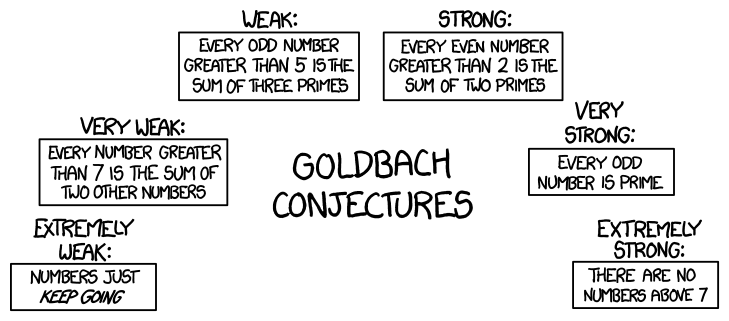
\includegraphics[width=0.5\textwidth]{background/pix/goldbach_conjectures.png}}
    \caption{Goldbach 的种种猜想。（致谢 \protect\href{https://xkcd.com/1310/}{\texttt{xkcd.com}}）}
    \label{fig:GoldbachsConjectures}
  \end{figure}
\end{answer}
\end{exercise}

\begin{exercise}
\definend{Brocard 问题}\index{Brocard's problem}
即是否存在除 $4$、$5$ 和~$7$ 以外的数，使得 $n!+1$ 是一个完全平方数
（计算机搜索最高已达
\citetext{一千万亿，即 $1\times 10^{15}$}{
  参见 \url{https://github.com/jhg023/brocard}.}，尚未发现其他解）。
证明：如果我们能够解决 \HP{}，那么我们原则上就能够判定这个问题。
\begin{answer}\verified
我们可以写一个程序，它接受输入，忽略输入，并执行一个循环来搜索大于~$7$ 的解，一旦找到就停机。
只要有了 \HP{} 的解法，我们就能检查该程序是否会停机，从而判定这个问题。
\end{answer}
\end{exercise}

% \begin{exercise}
% If we could solve the \HP{} then could we solve all problems?
% \begin{answer}
% No.
% \end{answer}
% \end{exercise}

\begin{exercise}
通过证明存在不可数无穷多个无法被任何 Turing 机计算的函数 $\map{f}{\N}{\N}$，而可计算的函数数量是可数的，来证明大多数问题都是不可解的。
\begin{answer}\verified
  所有函数 $\map{f}{\N}{\N}$ 的集合是两个子集的不交并：可计算的函数和不可计算的函数。
  我们知道可计算函数的集合是可数的。
  因为两个可数集的并集仍然是可数集，所以如果不可计算函数的集合也是可数的，那么总体上就只有可数多个函数，但事实并非如此。
  因此，不可计算函数的集合是不可数的。
\end{answer}
\end{exercise}

\begin{exercise}
给出一个全可计算函数（即对所有输入都收敛）的例子，使得其值域是不可计算的。
\begin{answer}
  固定一个元素 $k\in K$。
  以下函数 $\map{f}{\N^2}{\N}$ 的值域是~$K$。
  \begin{equation*}
    f(x,n)=
    \begin{cases}
    x  &\case{if $\TM_x$ with input~$x$ halts in $n$ steps}  \\
    k  &\case{otherwise}
    \end{cases}
  \end{equation*}
  显然该函数是可计算的，并且对所有输入对 $x,n\in\N^2$ 都收敛。
  对于 $K$ 的所有元素，都存在一个 $n$ 使得 $x$ 出现在值域中。
  同理，只有~$K$ 中的元素才会出现在值域中。
\end{answer}
\end{exercise}

\begin{exercise}
若一个比特串集合的特征函数是可计算的，则称其为
\definend{可判定语言}\index{decidable!language}\index{language!decidable}。
证明以下各条。
\begin{exparts*}
\item
两个可判定语言的并集是可判定语言。
\item
两个可判定语言的交集是可判定语言。
\item
一个可判定语言的补集是可判定语言。
\end{exparts*}
\begin{answer}\verified
  设有两个可判定语言~$\lang_0$ 和~$\lang_1$。
  因为它们是可判定的，所以存在 Turing 机 $\TM_{e_0}$ 和 $\TM_{e_1}$ 来判定其成员归属。
  \begin{equation*}
    \TMfcn_{e_0}(x)=
    \begin{cases}
      1  &\case{if $x\in\lang_0$}  \\
      0  &\case{if $x\notin\lang_0$}
    \end{cases}
    \qquad
    \TMfcn_{e_1}(x)=
    \begin{cases}
      1  &\case{if $x\in\lang_1$}  \\
      0  &\case{if $x\notin\lang_1$}
    \end{cases}
  \end{equation*}
  注意，这些机器在所有输入上都停机。
  \begin{figure}
    \centering
    \vcenteredhbox{\includegraphics{\asydir hp/hp1024.pdf}}
    \qquad
    \vcenteredhbox{\includegraphics{\asydir hp/hp1025.pdf}}
    \caption{判定可判定语言并集与交集的机器草图。}
    \label{fig:DecidableLangsUnionInt}
  \end{figure}
  \begin{exparts}
  \item
  判定 $\lang_0\cup\lang_1$ 成员资格的机器草图如 \figureref{fig:DecidableLangsUnionInt} 左侧所示。
  如果一个数是其中至少一个集合的成员，那么它就是并集的元素。
  因此，给定~$x$，这台机器首先在~$x$ 上运行 $\TM_{e_0}$。
  如果它返回~$1$，那么 $x$ 就是并集的成员，于是新机器输出~$1$。
  否则，新机器在~$x$ 上运行~$\TM_{e_1}$ 并返回其结果。
  \item
  判定 $\lang_0\cap\lang_1$ 成员资格的机器草图在同一图的右侧。
  如果一个数同时是这两个集合的成员，那么它就是交集的元素。
  因此，给定~$x$，这台机器首先在~$x$ 上运行 $\TM_{e_0}$。
  如果它返回~$0$，那么 $x$ 不是交集的成员，于是新机器输出~$0$。
  否则，新机器在~$x$ 上运行~$\TM_{e_1}$ 并返回其结果。
  \item
  补集的情况直截了当。
  对于~$\lang_0$ 的补集，新机器只需运行 $\TM_{e_0}$，并将其结果从~$1$ 中减去。
  \end{exparts}
\end{answer}
\end{exercise}


\end{exercises}
\index{Halting problem@\probname{Halting} problem|)}
\index{unsolvability|)}\index{unsolvable problem|)}

%================================================
\section{Rice 定理}\index{Rice's theorem|(}\label{sec:RicesThm}
我们在上一节最后指出，那里的结果和例子提供了一种直觉：我们无法
机械地分析 Turing 机的行为。
在本节中，我们将使这一直觉变得精确。

机械分析确实适用于 Turing 机的某些属性。
我们可以编写一个例程，给定~$e$，
判定 $\TM_e$ 是否有一条四元组指令，其第一项是状态~$q_5$。
在普通编程中，类似的情形是我们可以写一个程序来解析源代码，寻找名为 \str{x1} 的变量。
但这些并不是我们所说的“行为”。
相反，它们是实现层面的属性。

% A property is
% \definend{semantic}\index{semantic property}\index{property!semantic}
% if it has to do with the meaning of a thing; in our case,
% with what the machine does.\footnote{%
%   Often writers contrast these with properties that are
%   \definend{syntactic},\protect\index{syntactic property}\protect\index{property!syntactic}
%   which have to do with how a formal object is constructed.
%   We covered the syntax of Turing machines in the book's first section.}
% Briefly, a property is semantic if it is about $\TMfcn$ more than~$\TM\!$.
% For example,
% consider a Turing machine~$\TM$ that inputs a natural number and outputs~$1$
% if the number is prime and~$0$ otherwise.
% This machine's behavior is that it
% acts as the characteristic function of the set of primes.
% In contrast, suppose that it has a state~$q_5$ but no state~$q_6$.
% If we change all of the $q_5$'s in its transition table to some unused state
% such as $q_{1000}$'s
% then we get a different machine but the same behavior.

%<*def:SameBehavior>


\begin{definition}
两个可计算函数
\definend{具有相同行为，$\TMfcn_{e}\samebehavior\TMfcn_{\hat{e}}$}，\index{same behavior, functions with}\index{functions!same behavior}
如果它们在相同的输入~$x\in\N$ 上收敛，
且在收敛时具有相同的输出。\footnotemark[2]
\end{definition}

\footnotetext[2]{%
  严格来说，我们并不需要符号~$\samebehavior$。
  根据定义，函数是一个有序对的集合。
  如果
  $\TMfcn_e(0)\converges$ 而~$\TMfcn_e(1)\diverges$，那么集合 $\TMfcn_e$
  包含一个第一项为~$0$ 的有序对，但不包含任何第一项为~$1$ 的有序对。
  因此对于偏函数，如果它们在相同的输入上收敛，且在收敛时输出相同，那么我们可以直接说
  这两个函数相等，$\TMfcn=\hat{\TMfcn}$。
  但我们使用 $\samebehavior$ 来提醒自己这些函数可能是偏的。}
%</def:SameBehavior>

%<*def:IndexSet>


\begin{definition}
自然数集合 $\mathcal{I}$ 是一个
\definend{索引集}\footnotemark[1]\index{index set}\index{set!index}，
如果对所有~$e,\hat{e}\in\N$，
只要 $e\in\mathcal{I}$ 且 $\TMfcn_e\samebehavior\TMfcn_{\hat{e}}$，
则 $\hat{e}\in\mathcal{I}$ 也成立。
\end{definition}

\footnotetext[1]{%
  之所以称为索引集，是因为它是索引的集合。}
%</def:IndexSet>

\begin{example}
如果我们固定一种行为，并考虑所有具有该行为的 Turing 机
的索引，那么我们就得到了一个索引集。
因此，集合
$\mathcal{I}=\set{e\in\N\suchthat \text{$\phi_e(x)=2x$ for all $x$}}$
是一个索引集。
为了验证，假设 $e\in\mathcal{I}$ 且 $\hat{e}\in\N$ 满足
$\phi_e\samebehavior \phi_{\hat{e}}$。
那么 $\phi_{\hat{e}}$ 也将其输入翻倍：$\phi_{\hat{e}}(x)=2x$ 对所有~$x$ 成立。
因此 $\hat{e}\in\mathcal{I}$ 也成立。
\end{example}

\begin{example} \label{ex:IndexSetMultipleBehaviors}
我们也可以通过收集多种行为来得到一个索引集。
集合
$\mathcal{J}=\set{e\in\N\suchthat
      \text{$\phi_e(x)=3x$ for all $x$, or $\phi_e(x)=x^3$ for all~$x$}}
$
是一个索引集。
因为，假设 $e\in\mathcal{J}$ 且
$\phi_e\samebehavior \phi_{\hat{e}}$，其中 $\hat{e}\in\N$。
由于 $e\in\mathcal{J}\!$，要么
$\phi_e(x)=3x$ 对所有 $x$ 成立，要么 $\phi_e(x)=x^3$ 对所有~$x$ 成立。
从 $\phi_e\samebehavior \phi_{\hat{e}}$ 我们知道，
要么 $\phi_e(x)=3x$ 对所有 $x$ 成立，要么 $\phi_e(x)=x^3$ 对所有~$x$ 成立，从而
$\hat{e}\in\mathcal{J}\!$。
\end{example}

\begin{example} \label{ex:NotIndexSet}
集合 $\set{e\in\N\suchthat
      \text{$\TM_e$ contains an instruction starting with $q_{10}$}}$
不是一个索引集。
我们可以很容易地构造两台行为相同的 Turing 机，
其中一台包含这样一条指令，而另一台不包含。
\end{example}

%<*th:RicesTheorem>


\begin{theorem}[Rice 定理]\index{Rice's theorem}   \label{thm:RicesThm}
每个非平凡的索引集（即非空且不是全体自然数集~$\N$）都是不可计算的。
\end{theorem}


%</th:RicesTheorem>

\begin{proof}
%<*pf:RicesTheoremi>
设 $\mathcal{I}$ 是一个非平凡的索引集。
选取 $e\in\N$，使得 $\TMfcn_{e}(y)\diverges$ 对所有 $y$ 成立。
那么要么 $e\in\mathcal{I}$，要么 $e\notin\mathcal{I}$。
我们将证明在第二种情况下 $\mathcal{I}$ 是不可计算的。
第一种情况类似，留作练习~\zcref{exer:OtherHalfRicesThm}。

所以假设 $e\notin\mathcal{I}$。
由于 $\mathcal{I}$ 非空，它包含一个索引 $\hat{e}\in\mathcal{I}$。
因为 $\mathcal{I}$ 是一个索引集，$\TMfcn_{e}\not\simeq\TMfcn_{\hat{e}}$。
因此存在一个 $y$ 使得 $\TMfcn_{\hat{e}}(y)\converges$。

考虑下面的左流程图。
根据 Church 论题，存在一台具有该行为的 Turing 机。
记其为 $\TM_{e_0}$。
应用 \smn{} 定理将 $x$ 参数化，
得到一致可计算的函数族 $\TMfcn_{s(e_0,x)}$，其计算过程如右图所示。
%</pf:RicesTheoremi>
\begin{center}
  \vcenteredhbox{\includegraphics{\asydir hp/hp12.pdf}}
  \hspace{4em}
  \vcenteredhbox{\includegraphics{\asydir hp/hp13.pdf}}
\end{center}
%<*pf:RicesTheoremii>
我们构造了右边的机器，使得如果
$\TMfcn_x(x)\diverges$，那么 $\TMfcn_{s(e_0,x)}\samebehavior\TMfcn_{e}$，
从而 $s(e_0,x)\notin\mathcal{I}$。
同样，
如果 $\TMfcn_x(x)\converges$，那么 $\TMfcn_{s(e_0,x)}\samebehavior\TMfcn_{\hat{e}}$，
从而 $s(e_0,x)\in\mathcal{I}$。
由此可得，如果 $\mathcal{I}$ 是机械可计算的，从而我们能
有效检查是否 $s(e_0,x)\in\mathcal{I}$，
那么我们就能解决停机问题。
%</pf:RicesTheoremii>
\end{proof}

\begin{example}
我们将使用 Rice 定理证明此问题不可解：给定
$e$，判定 $\TMfcn_e(3)\converges$ 是否成立。
我们必须定义一个适当的集合~$\mathcal{I}$，然后验证它非空、
不等于全体自然数集，并且是一个索引集。

令
$
  \mathcal{I}=\set{e\in\N \suchthat \TMfcn_e(3)\converges}
$。
验证该集合非空的最简单方法是给出一个成员。
下面左侧的例程直觉上是可计算的，因此
根据 Church 论题，存在一台具有该行为的 Turing 机。
那台机器的索引是 $\mathcal{I}$ 的一个成员，
从而 $\mathcal{I}\neq\emptyset$。
\begin{center}
  \vcenteredhbox{\includegraphics{\asydir hp/hp1052.pdf}}
  \hspace{6em}
  \vcenteredhbox{\includegraphics{\asydir hp/hp1053.pdf}}
\end{center}
同样，为了验证 $\mathcal{I}$ 不包含每个数，
考虑右侧的例程。
Church 论题表明，存在一台具有该行为的 Turing 机。
那台机器的索引不是 $\mathcal{I}$ 的成员，
因此 $\mathcal{I}\neq\N$。

我们最后验证 $\mathcal{I}$ 是一个索引集。
假设 $e\in\mathcal{I}$，并令 $\hat{e}\in\N$ 满足 $\TMfcn_e\samebehavior\TMfcn_{\hat{e}}$。
由于 $e\in\mathcal{I}$，我们有 $\TMfcn_e(3)\converges$。
因为 $\TMfcn_e\samebehavior\TMfcn_{\hat{e}}$，我们也有
$\TMfcn_{\hat{e}}(3)\converges$，从而
$\hat{e}\in\mathcal{I}$。
因此 $\mathcal{I}$ 是一个索引集。
\end{example}

上面的例子与前一子节的第一个例子是同一个问题。
Rice 定理极大地简化了答案。
（当然，我们对这一定理的推导依赖于前节的工作。）

\begin{example}
我们可以用 Rice 定理来证明前一节的第二个问题不可解：给定 $e$，
判定是否存在某个 $x$ 使得 $\phi_e(x)=7$。
我们将构造一个适当的 $\mathcal{I}$
并验证它是一个非平凡的索引集。

令
$\mathcal{I}=\set{e\in\N \suchthat \text{$\TMfcn_e(x)=7$ for some $x$}}$。
这个集合非空，因为存在一台 Turing 机作为恒等函数，
即 $\TMfcn(x)=x$，
那台机器的索引是 $\mathcal{I}$ 的一个成员。
这个集合不等于全体自然数集，因为
存在一台永不停机的 Turing 机，对所有 $x$ 都有 $\TMfcn(x)\diverges$，
那台机器的索引不是 $\mathcal{I}$ 的成员。
因此 $\mathcal{I}$ 是非平凡的。

为了证明 $\mathcal{I}$ 是一个索引集，
假设 $e\in\mathcal{I}$，并令 $\hat{e}\in\N$ 满足
$\TMfcn_e\samebehavior\TMfcn_{\hat{e}}$。
由假设，存在某个输入 $x_0$ 使得 $\TMfcn_e(x_0)=7$。
由于两者具有相同行为，相同的输入会给出
$\TMfcn_{\hat{e}}(x_0)=7$。
因此，$\hat{e}\in\mathcal{I}$。
\end{example}

\begin{example}
这里是另一个不可解问题：给定~$e$，判定 $\TMfcn_e$ 是否等于 \begin{equation*}
  f(x)=
  \begin{cases}
    4  &\case{if $x$ is prime}  \\
    x+1 &\case{otherwise}
  \end{cases}
\end{equation*}。
令$\mathcal{I}=\set{j\in\N\suchthat \TMfcn_j=f}$。
集合~$\mathcal{I}$ 非空，因为我们可以写出具有这种行为的程序，因此根据 Church 论题，存在具有这种行为的 Turing 机，其索引就是~$\mathcal{I}$ 中的成员。
同时，$\mathcal{I}\neq\N$，因为存在一台在任何输入上都不停机的 Turing 机，它的索引不是~$\mathcal{I}$ 的成员。

为完成证明，我们论证~$\mathcal{I}$ 是一个索引集。
假设 $e\in\mathcal{I}$ 并且 $\hat{e}$ 满足 $\TMfcn_e\samebehavior\TMfcn_{\hat{e}}$。
因为 $e\in\mathcal{I}$，所以对所有输入~$x$ 均有 $\TMfcn_e(x)=f(x)$。
由于 $\TMfcn_e\samebehavior\TMfcn_{\hat{e}}$，我们对所有~$x$ 均有 $\TMfcn_{\hat{e}}(x)=\TMfcn_{e}(x)$，因此 $\hat{e}$ 也是~$\mathcal{I}$ 中的成员。
所以 $\mathcal{I}$ 是一个索引集。
\end{example}

最后，我们从一个稍高的层次重新审视这一定理。
本章首先展示了不可解问题是存在的。
然而，那个基于计数的证明并没有给出自然的例子。
在上一节中，我们得到了许多有趣且实用的不可解问题的例子，
这些例子让我们直观地认识到，我们无法机械地分析机器的行为。
本节我们形式化地定义了“行为”。
在此基础上，
Rice 定理指出，每一个有意义的行为集合，
即每一个非平凡索引集，都是不可解的。
因此，我们起初觉得不可解问题十分离奇，
接着认识到它们确实会出现，
直到现在，如果粗略地解读，甚至可能会让人觉得所有问题都是不可解的。

但这显然不对。
我们都编写过处理现实世界任务的程序，对于这些程序的行为，我们至少会非正式地认为它们是有趣的。
要化解这一矛盾，当然需要认识到 Rice 定理指出的只是：只有当问题属于特定类型时才是不可解的。
我们现在就来详述这种类型。

在下方的左图中，红点代表 Turing 机。
（当然机器的数量是无限的，但这只是一个示意图。）
有些成对的机器具有相同的输入/输出行为，也就是说它们
产生相同的可计算函数。\footnote{%
  实际上，第~\protect\pageref{lem:EveryCompFcnHasInfManyIndices}~页的 Padding 引理
  指出对于每个可计算函数都存在无穷多台机器。}
因此，存在多台机器其输入/输出行为是加倍函数 $f(x)=2x$，
多台机器在任何输入上都不停机，
等等。
图中的瓦片将具有相同行为、给出相同可计算函数的机器分在一组。


\begin{center}
  \includegraphics{\asydir indexsets/indexsets002.pdf}%
  \hspace*{4em}
  \includegraphics{\asydir indexsets/indexsets003.pdf}%
\end{center}

如果每当两台机器计算同一函数时——即每当它们出现在
同一块瓦片中时——它们要么都具有该性质，
要么都不具有，我们就说机器的这个性质是
\citetext{外延的}{%
  这个说法源自 A~Bauer，见 \url{https://cs.stackexchange.com/q/2811/67754}。\index{extensional property}
}。
Rice 定理断言，一个有效的（即可计算的）机器外延性质必须是平凡的，也就是说，它要么对所有机器都成立，要么对所有机器都不成立。

以下是机器的一些外延性质：


\begin{parenum}
\item 在输入~$3$ 上停机，
\item 存在一个输入使得输出为~$7$，
\item 存在一个输入使得机器不停机。
\end{parenum}


例如对于~(1)，由于它是一个
外延性质且非平凡，Rice 定理指出它不可能是
有效的，我们无法可计算地判定它。

以下是一些非外延性质，
Rice 定理对它们不适用：


\begin{parenum}
\item 在每个输入上都在 $100$ 步内停机，
\item 在输入~$0$ 上访问少于~$100$ 个带方格，以及
\item 包含状态~$q_{10}$。
\end{parenum}

那么，如果每个瓦片代表一种行为，什么是索引集呢？
正如我们之前所见，例如在 \zcref{ex:IndexSetMultipleBehaviors} 中，
一个索引集是多个瓦片的索引的并集；
右上方的图合并了其中的三个瓦片。
属于这个~$\mathcal{I}$ 这一性质是外延的，因为我们取的是
完整的瓦片。

总而言之，尽管 Rice 定理并不适用于所有问题，
但它对于理解仅凭机械分析能做什么具有特别重要的意义。
Rice 定理关注的是机器的这样一类性质，它们可以推广为机器所计算函数的性质。
例如，判定一个程序是否计算平方函数的问题是不可解的，
但判定其源代码是否包含字母 ‘\str{k}’ 的问题则不是。

% ...................................................
\begin{exercises}
% possible: https://cs.stackexchange.com/q/117066/50343

\begin{exercise}
你的朋友感到困惑，“根据 Rice 定理，所有事情都是不可能的。
计算机程序的每个性质都是不可计算的。
但我却一直在做这些本该不可能的事情！”
请帮他理清头绪。
\begin{credit}
  问题来自 StackExchange 用户 MathematicalOrchid，
  \url{https://cs.stackexchange.com/q/2811/67754},
  本节使用了 StackExchange 用户 Andrej Bauer 的答案。
  此处的答案并非来自 Andrej Bauer。
\end{credit}
\begin{answer}\verified
Rice 定理并没有说所有事情都是不可能的。
例如，它并没有说编写一个实现 $f(x)=x^2$ 的例程是不可能的。

它所断言不可能的事情是：编写一个例程，在给定源代码后，
能够正确判定这段源代码（无论写得多么巧妙，或故意混淆得多么晦涩）是否实现了~$f$。
（这种判定器之所以有意义，是因为我们可以把它应用到第一段提到的那个例程上，
从而确切地知道它在所有情况下都能正确工作。）
\end{answer}
\end{exercise}

\begin{exercise}
$\mathcal{I}=\set{e\suchthat \text{$\TM_e$ runs for at least $100$ steps on input~$5$}}$
是索引集吗？
\begin{answer}\verified
  不是，它不是索引集。
  我们可以写出两台行为相同的 Turing 机，例如，对任何输入~$x$，它们都输出~$x$。
  其中一台只需要很少几步就能做到这一点
  （平凡的 Turing 机~$\TM=\set{}$ 甚至只需零步），
  而另一台需要 $101$ 步。
  第二台机器的索引属于~$\mathcal{I}$，但第一台机器的索引不属于。
\end{answer}
\end{exercise}

\begin{exercise}
为什么 Rice 定理没有表明这个问题是不可解的：给定~$e$，判定是否
$\emptyset\subseteq\set{x\suchthat \TMfcn_e(x)\converges}$？
\begin{answer}\verified
使得
$\emptyset\subseteq\set{x\suchthat \TMfcn_e(x)\converges}$
成立的索引~$e\in\N$ 的集合是整个 $\N$。
这个问题是可解的，尽管其解是平凡的：对任何~$e$，答案都是“是”。
\end{answer}
\end{exercise}

\begin{exercise}
判断真假：以下关于机器的性质是外延的吗？简要说明理由。
\begin{exparts*}
\item 机器在输入~$5$ 上停机。
\item 它恰好有四条指令。
\item 它计算其输入的两倍。
\end{exparts*}
\begin{answer}\verified
\begin{exparts}
\item 真，这是关于机器的输入/输出行为的。
  如果两台机器具有相同的输入/输出行为，并且其中一台在输入~$5$ 上停机，
  那么另一台也必然如此。
\item 假，我们可以造出两台行为相同，但其中一台有四条指令而另一台没有四条指令的机器。
  例如，我们可以拿一台有四条指令的机器，然后通过添加不可达代码来造一台新机器，
  这些无实际作用的指令以原四条指令未曾引用过的状态为起始状态。
\item 真。
  如果两台机器计算相同的函数，并且第一台机器的函数是 $x\mapsto 2x$，
  那么第二台机器的函数也是如此。
\end{exparts}
\end{answer}
\end{exercise}

\begin{exercise}
简要说明为何本节列出的这些机器性质是非外延的。
\begin{exparts*}
\item 在任何输入上都能在 $100$ 步内停机的性质，
\item 在输入~$0$ 时访问少于~$100$ 个带方格的性质，以及
\item 包含状态~$q_{10}$ 的性质。
\end{exparts*}
\begin{answer}\verified
在每种情况下，我们都将论证：存在两台机器 $\TM$ 和~$\hat{\TM}$，
它们具有相同的输入/输出行为，$\TMfcn=\hat{\TMfcn}$，但其中一台机器具有该性质而另一台没有。
\begin{exparts}
\item 平凡的 Turing 机 $\TM=\set{}$ 在零步内停机，其行为是 $\TMfcn(x)=x$。
  我们可以轻易地造出另一台具有相同行为，但耗费超过一百步的机器。
\begin{equation*}
  \hat{\TM}=\set{
       \tminstruction{0}{B}{B}{1},
       \tminstruction{0}{1}{1}{1},
       \tminstruction{1}{B}{B}{2},
       \tminstruction{1}{1}{1}{2},
       \ldots\,
       \tminstruction{100}{B}{B}{101},
       \tminstruction{100}{1}{1}{101}
     }
\end{equation*}
\item 与上一条类似，平凡的机器在输入~$0$ 时使用零个带方格。
  下面这台机器在输入~$0$ 时访问一百零一个带方格。
\begin{equation*}
  \hat{\TM}=\set{
       \tminstruction{0}{B}{L}{1},
       \tminstruction{0}{1}{1}{102},
       \tminstruction{1}{B}{L}{2},
       \tminstruction{1}{1}{L}{2},
       \ldots\,
       \tminstruction{100}{B}{L}{101},
       \tminstruction{100}{1}{L}{101}
     }
\end{equation*}
  两台机器的行为相同，都是 $\TMfcn(x)=x$。
\item 平凡的机器不包含任何带有状态~$q_{10}$ 的指令。
  下面这台机器
\begin{equation*}
  \hat{\TM}=\set{\tminstruction{0}{B}{B}{1},
        \tminstruction{0}{1}{1}{1},
        \tminstruction{1}{B}{B}{2},
        \tminstruction{1}{1}{1}{2},
        \ldots\,
        \tminstruction{10}{B}{B}{11},
        \tminstruction{10}{1}{1}{11}
      }
\end{equation*}
  具有相同的行为，并且包含一条带有该状态的指令。
\end{exparts}
\end{answer}
\end{exercise}

\begin{exercise}
构造一个平凡的索引集：填空
$\mathcal{I}=\set{e\suchthat \text{\underline{\makebox[3em]{}}$\TM_e$\underline{\makebox[3em]{}}}}$
使得集合~$\mathcal{I}$ 是空集。
\begin{answer}\verified
  描述空集的方式有很多。
  一种是 $\set{e\suchthat \text{$\TM_e$ solves the \HP}}$。
\end{answer}
\end{exercise}

\begin{exercise}
构造一个平凡的索引集：填空
$\mathcal{I}=\set{e\suchthat \text{\underline{\makebox[3em]{}}$\TM_e$\underline{\makebox[3em]{}}}}$
使得集合~$\mathcal{I}$ 是整个 $\N$。
\begin{answer}\verified
  描述所有索引的集合~$\N$ 的一种方式是 $\set{e\suchthat \text{on input~$3$ machine $\TM_e$ either halts or does not}}$。
\end{answer}
\end{exercise}

\begin{exercise}
对于下列每个问题，构造一个适用于 Rice 定理的索引集。
你无需给出完整论证，只需给出这个集合即可。
\begin{exparts}
\item 给定 $e$，判断 $\TM_e$ 在输入 $7$ 上是否停机且输出 $7\!$。
\item 给定 $e$，判断 $\TM_e$ 在输入~$e$ 上是否停机且输出~$e$。
\item 给定 $e$，判断 $\TM_{2e}$ 是否对任意输入~$y$ 都输出 $7$。
\item 给定 $e$，判断 $\TM_e$ 在输入 $7$ 上是否停机并输出一个素数。
\end{exparts}
\begin{answer}\verified
记号 $\TMfcn_e(x)=y$ 表示 $\TMfcn_e(x)$ 收敛且输出值为~$y$。
\begin{exparts}
\item $\set{e\in\N\suchthat \text{$\TMfcn_e(7)=7$}}$
\item $\set{e\in\N\suchthat \text{$\TMfcn_e(e)=e$}}$
\item $\set{e\in\N\suchthat \text{there is a $y$ where $\TMfcn_{2e}(y)=7$}}$
\item $\set{e\in\N\suchthat \text{$\TMfcn_e(7)\converges$ and is prime}}$
\end{exparts}
\end{answer}
\end{exercise}

\exerciseinstructions{对于 \zcref{exer:FirstRiceExercise} 到 \zcref{exer:FinalRiceExercise} 中的每个问题，通过应用 Rice 定理来证明它是不可解的。（这些问题重复了 \zcref{exer:FirstReduceExercise} 到 \zcref{exer:FinalReduceExercise} 的问题。）}

\recommended


\begin{exercise}\label{exer:FirstRiceExercise}
\refexerciseinstructions{}
给定
索引~$e$，
判断 $\TMfcn_e$ 是否为全函数，即它是否在每个输入上都收敛。
\begin{answer}\verified
令 $\mathcal{I}=\set{e\in\N\suchthat\text{$\TMfcn_e$ is total}}$。
我们将证明它是一个非平凡的索引集。

首先证明~$\mathcal{I}$ 不是空集。
考虑 \figureref{fig:INotTrivialTotalFcnsNotComputable} 左侧草图所示的程序。
  \begin{figure}
    \centering
    \vcenteredhbox{\includegraphics{\asydir hp/hp1028.pdf}}
    \hspace*{4em}
    \vcenteredhbox{\includegraphics{\asydir hp/hp1029.pdf}}
    \caption{用于证明集合~$\mathcal{I}$ 非平凡的机器。}
    \label{fig:INotTrivialTotalFcnsNotComputable}
  \end{figure}
根据 Church 论题，存在一台符合此草图的 Turing 机。
它有一个索引，且该索引是~$\mathcal{I}$ 的元素。
所以 $\mathcal{I}$ 非空。

接下来证明~$\mathcal{I}$ 不是整个~$\N$。
考虑同一图右侧草图所示的程序。
根据 Church 论题，存在一台符合此草图的 Turing 机。
它的索引不是~$\mathcal{I}$ 的元素，因此
$\mathcal{I}$ 不是整个~$\N$。

最后，我们证明 $\mathcal{I}$ 是一个索引集。
假设 $e\in\mathcal{I}$ 且 $\hat{e}$ 满足 $\TMfcn_e\samebehavior\TMfcn_{\hat{e}}$。
因为 $e\in\mathcal{I}$，
我们知道对所有的 $a\in\N$ 有 $\TMfcn_e(a)\converges$。
由于 $\TMfcn_x\samebehavior\TMfcn_{\hat{e}}$，我们因此知道
对所有的 $a\in\N$ 有 $\TMfcn_{\hat{e}}(a)\converges$。
于是，$\hat{e}\in\mathcal{I}$，从而
$\mathcal{I}$ 是一个索引集。

因此，Rice 定理表明，
判定“全函数性”的问题，即给定~$e$ 时判定
Turing 机~$\TM_e$ 是否在所有输入上停机的问题，
是不可解的。
\end{answer}
\end{exercise}

\recommended


\begin{exercise}
\refexerciseinstructions[exer:FirstRiceExercise]
给定索引~$e$，判定 Turing 机~$\TM_e$ 是否计算其输入的平方。
也就是说，判定 $\TMfcn_e$ 是否实现映射 $y\mapsto y^2$。
\begin{answer}\verified
令 $\mathcal{I}=\set{e\in\N\suchthat\text{$\TMfcn_e(y)=y^2$ for all $y$}}$。
我们将证明它是一个非平凡的索引集。

首先证明~$\mathcal{I}$ 不是空集。
考虑 \figureref{fig:INotTrivialSquarerFcnsNotComputable} 左侧草图所示的程序。
  \begin{figure}
    \centering
    \vcenteredhbox{\includegraphics{\asydir hp/hp1030.pdf}}
    \hspace*{4em}
    \vcenteredhbox{\includegraphics{\asydir hp/hp1031.pdf}}
    \caption{用于证明平方函数的索引集 $\mathcal{I}$ 非平凡的机器。}
    \label{fig:INotTrivialSquarerFcnsNotComputable}
  \end{figure}
根据 Church 论题，存在一台符合此草图的 Turing 机。
它有一个索引，且该索引是~$\mathcal{I}$ 的元素。
所以 $\mathcal{I}$ 非空。

接下来证明~$\mathcal{I}$ 不是整个~$\N$。
考虑同一图右侧草图所示的程序。
根据 Church 论题，存在一台符合此草图的 Turing 机。
它的索引不是~$\mathcal{I}$ 的元素，因此
$\mathcal{I}$ 不是整个~$\N$。

最后我们证明 $\mathcal{I}$ 是一个索引集。
假设 $e\in\mathcal{I}$ 且 $\hat{e}$ 满足 $\TMfcn_e\samebehavior\TMfcn_{\hat{e}}$。
因为 $e\in\mathcal{I}$，
我们知道对所有 $y\in\N$ 有 $\TMfcn_e(y)=y^2$。
由于 $\TMfcn_e\samebehavior\TMfcn_{\hat{e}}$，我们因此知道
对所有 $y\in\N$ 有 $\TMfcn_{\hat{e}}(y)=y^2$。
于是，$\hat{e}\in\mathcal{I}$，从而
$\mathcal{I}$ 是一个索引集。

由此，Rice 定理表明，
给定~$e$，判定 Turing 机~$\TM_e$ 是否计算其输入的平方的问题，
是不可解的。
\end{answer}
\end{exercise}

\begin{exercise}
\refexerciseinstructions[exer:FirstRiceExercise]
给定~$e$，确定函数~$\TMfcn_e$ 是否在两个相邻输入上返回相同的值，
即存在某个~$y\in\N$ 使得 $\TMfcn_e(y)=\TMfcn_e(y+1)$。
\begin{answer}\verified
我们将证明
$\mathcal{I}=\set{e\in\N\suchthat\text{$\TMfcn_e(y)=\TMfcn_e(y+1)$ for some $y\in\N$}}$
是一个非平凡的索引集。

首先证明~$\mathcal{I}$ 非空。
考虑 \figureref{fig:IRepeatedValueFcnNotTrivial} 左侧草图所示的程序。
  \begin{figure}
    \centering
    \vcenteredhbox{\includegraphics{\asydir hp/hp1028.pdf}}
    \hspace*{4em}
    \vcenteredhbox{\includegraphics{\asydir hp/hp1029.pdf}}
    \caption{用于证明集合~$\mathcal{I}$ 非平凡的机器。}
    \label{fig:IRepeatedValueFcnNotTrivial}
  \end{figure}
它在直观上是可计算的，因此根据 Church 论题，存在一台符合此草图的 Turing 机。
该 Turing 机的索引是~$\mathcal{I}$ 的一个元素。
所以 $\mathcal{I}$ 非空。

接下来论证~$\mathcal{I}\neq\N$。
考虑同一图右侧草图所示的程序。
根据 Church 论题，存在一台符合此草图的 Turing 机。
它的索引不是~$\mathcal{I}$ 的元素，因此 $\mathcal{I}$ 不是整个~$\N$。

最后，证明 $\mathcal{I}$ 是一个索引集。
假设 $e\in\mathcal{I}$，并且 $\hat{e}$ 满足 $\TMfcn_e\samebehavior\TMfcn_{\hat{e}}$。
因为 $e\in\mathcal{I}$，存在 $y\in\N$ 使得 $\TMfcn_e(y)=\TMfcn_e(y+1)$。
由于 $\TMfcn_e\samebehavior\TMfcn_{\hat{e}}$，我们知道对于同一个~$y$，有 $\TMfcn_{\hat{e}}(y)=\TMfcn_{\hat{e}}(y+1)$。
因此，$\hat{e}\in\mathcal{I}$。
所以 $\mathcal{I}$ 是一个索引集。

于是，根据 Rice 定理，
判定是否属于 $\mathcal{I}$ 的问题是不可解的。
\end{answer}
\end{exercise}

\begin{exercise}
\refexerciseinstructions[exer:FirstRiceExercise]
给定索引~$e$，确定 $\TMfcn_e$ 在输入~$5$ 上是否发散。
\begin{answer}\verified
我们将证明
$\mathcal{I}=\set{e\in\N\suchthat\TMfcn_e(5)\diverges}$
是一个非平凡的索引集。

首先证明~$\mathcal{I}\neq\emptyset$。
考虑 \figureref{fig:IDivergesOnFiveNotTrivial} 左侧草图所示的程序。
  \begin{figure}
    \centering
    \vcenteredhbox{\includegraphics{\asydir hp/hp1029.pdf}}
    \hspace*{4em}
    \vcenteredhbox{\includegraphics{\asydir hp/hp1028.pdf}}
    \caption{用于证明~$\mathcal{I}$ 非平凡的 Turing 机草图。}
    \label{fig:IDivergesOnFiveNotTrivial}
  \end{figure}
它在直观上是可计算的，因此根据 Church 论题，存在一台符合此草图的 Turing 机。
该机器的索引是~$\mathcal{I}$ 的一个元素。

接下来论证~$\mathcal{I}\neq\N$。
考虑同一图右侧草图所示的程序。
根据 Church 论题，存在一台符合此草图的 Turing 机。
它的索引不是~$\mathcal{I}$ 的元素。

最后，证明 $\mathcal{I}$ 是一个索引集。
假设 $e\in\mathcal{I}$，并且 $\hat{e}$ 满足 $\TMfcn_e\samebehavior\TMfcn_{\hat{e}}$。
因为 $e\in\mathcal{I}$，我们知道 $\TMfcn_e(5)\diverges$。
但 $\TMfcn_e\samebehavior\TMfcn_{\hat{e}}$，所以我们也有 $\TMfcn_{\hat{e}}(5)\diverges$。
因此，$\hat{e}\in\mathcal{I}$。
所以 $\mathcal{I}$ 是一个索引集。

由此，Rice 定理表明判定是否属于 $\mathcal{I}$ 的问题是不可解的。
\end{answer}
\end{exercise}

\begin{exercise}
\refexerciseinstructions[exer:FirstRiceExercise]
给定一个索引，确定 Turing 机 $\TM_e$ 是否在所有奇数上均不停机。
\begin{answer}\verified
我们将证明
$\mathcal{I}=\set{e\in\N\suchthat\text{$\TMfcn_e(y)\diverges$ for all odd~$y$}}$
是一个非平凡的索引集。

首先证明~$\mathcal{I}\neq\emptyset$。
考虑 \figureref{fig:IDivergesOnOddNotTrivial} 左侧草图所示的程序。
  \begin{figure}
    \centering
    \vcenteredhbox{\includegraphics{\asydir hp/hp1029.pdf}}
    \hspace*{4em}
    \vcenteredhbox{\includegraphics{\asydir hp/hp1028.pdf}}
    \caption{用于证明~$\mathcal{I}$ 非平凡的机器。}
    \label{fig:IDivergesOnOddNotTrivial}
  \end{figure}
它在直观上是可计算的，因此根据 Church 论题，存在一台符合此草图的 Turing 机。
该机器的索引是~$\mathcal{I}$ 的一个元素。

接下来验证~$\mathcal{I}\neq\N$。
考虑同一图右侧草图所示的程序。
根据 Church 论题，存在一台符合此草图的 Turing 机。
它的索引不是~$\mathcal{I}$ 的元素。

最后，证明 $\mathcal{I}$ 是一个索引集。
假设 $e\in\mathcal{I}$，并且 $\hat{e}$ 满足 $\TMfcn_e\samebehavior\TMfcn_{\hat{e}}$。
因为 $e\in\mathcal{I}$，我们知道对于所有奇数输入~$y$，$\TMfcn_e(y)\diverges$。
由于 $\TMfcn_e\samebehavior\TMfcn_{\hat{e}}$，我们也知道对于所有奇数~$y$，$\TMfcn_{\hat{e}}(y)\diverges$。
因此，$\hat{e}\in\mathcal{I}$，
所以 $\mathcal{I}$ 是一个索引集。

由此，Rice 定理表明判定是否属于 $\mathcal{I}$ 的问题是不可解的。
\end{answer}
\end{exercise}

\begin{exercise}
\refexerciseinstructions[exer:FirstRiceExercise]
给定索引~$e$，判断由机器~$\TM_e$ 计算的函数~$\phi_e$ 是否实现映射 $x\mapsto x+1$。
\begin{answer}\verified
我们将证明
$\mathcal{I}=\set{e\in\N\suchthat\TMfcn_e(x)=x+1}$
是一个非平凡的索引集。

首先证明~$\mathcal{I}\neq\emptyset$。
考虑 \figureref{fig:ISuccessorNotTrivial} 左侧的程序草图。
  \begin{figure}
    \centering
    \vcenteredhbox{\includegraphics{\asydir hp/hp1032.pdf}}
    \hspace*{4em}
    \vcenteredhbox{\includegraphics{\asydir hp/hp1033.pdf}}
    \caption{用于证明~$\mathcal{I}$ 非平凡的机器。}
    \label{fig:ISuccessorNotTrivial}
  \end{figure}
它直观上是可计算的，因此由 Church 论题，存在一台 Turing 机符合此草图。
该机器的索引是~$\mathcal{I}$ 的一个元素。

接着证明~$\mathcal{I}\neq\N$。
考虑该图右侧的程序草图。
由 Church 论题，存在一台 Turing 机符合此草图。
它的索引不是~$\mathcal{I}$ 的元素。

最后证明 $\mathcal{I}$ 是一个索引集。
假设 $e\in\mathcal{I}$ 并且 $\hat{e}$ 满足
$\TMfcn_e\samebehavior\TMfcn_{\hat{e}}$。
因为 $e\in\mathcal{I}$，我们知道对所有输入~$x$ 都有 $\TMfcn_e(x)=x+1$。
由于 $\TMfcn_e\samebehavior\TMfcn_{\hat{e}}$，我们也知道
$\TMfcn_{\hat{e}}(x)=x+1$ 对所有~$x$ 成立。
因此，$\hat{e}\in\mathcal{I}$。
所以 $\mathcal{I}$ 是一个索引集。

于是，由 Rice 定理，
判定~$\mathcal{I}$ 的成员资格问题是不可解的。
\end{answer}
\end{exercise}

\begin{exercise} \label{exer:FinalRiceExercise}
\refexerciseinstructions[exer:FirstRiceExercise]
给定索引~$e$，判断函数~$\phi_e$ 是否对某个~$x$，在输入 $x$ 和~$2x$ 上均发散。
\begin{answer}\verified
我们将证明
$\mathcal{I}=\set{e\in\N\suchthat\text{both $\TMfcn_e(x)\diverges$ and $\TMfcn_e(2x)\diverges$ for some~$x$}}$
是一个非平凡的索引集。

首先证明~$\mathcal{I}\neq\emptyset$。
考虑 \figureref{fig:IDivergesOnXAndTwoXNotTrivial} 左侧的程序草图。
  \begin{figure}
    \centering
    \vcenteredhbox{\includegraphics{\asydir hp/hp1034.pdf}}
    \qquad
    \vcenteredhbox{\includegraphics{\asydir hp/hp1035.pdf}}
    \caption{用于证明~$\mathcal{I}$ 非平凡的机器。}
    \label{fig:IDivergesOnXAndTwoXNotTrivial}
  \end{figure}
它直观上是可计算的，因此由 Church 论题，存在一台 Turing 机符合此草图。
该机器的索引是~$\mathcal{I}$ 的一个元素。

接着证明~$\mathcal{I}\neq\N$。
考虑 \figureref{fig:IDivergesOnXAndTwoXNotTrivial} 右侧的程序草图。
由 Church 论题，存在一台 Turing 机符合此草图。
它的索引不是~$\mathcal{I}$ 的元素。

最后证明 $\mathcal{I}$ 是一个索引集。
假设 $e\in\mathcal{I}$ 并且 $\hat{e}$ 满足
$\TMfcn_e\samebehavior\TMfcn_{\hat{e}}$。
因为 $e\in\mathcal{I}$，我们知道存在某个输入~$x$，使得 $\TMfcn_e(x)\diverges$ 且 $\TMfcn_e(2x)\diverges$。
由于 $\TMfcn_e\samebehavior\TMfcn_{\hat{e}}$，我们知道对同一个~$x$，
$\TMfcn_{\hat{e}}(x)\diverges$ 且 $\TMfcn_{\hat{e}}(2x)\diverges$。
因此，$\hat{e}\in\mathcal{I}$。
所以 $\mathcal{I}$ 是一个索引集。

于是，由 Rice 定理，
判定~$\mathcal{I}$ 的成员资格问题是不可解的。
\end{answer}
\end{exercise}

\recommended


\begin{exercise}
应用 Rice 定理，证明下列每个问题都是不可解的。
\begin{exparts}
\item 判定一个函数是否为偏函数，即该函数是否在某个输入上发散。
\item 判定一个函数是否至少在某个输入上收敛。
\end{exparts}
\begin{answer}\verified
第一小题中的索引集，是 \ref{exer:FirstRiceExercise} 中那个索引集的补集。
  后续练习 \ref{exer:IndexSetsClosedSetOps} 会证明，索引集的补集也是索引集。
  但下面我们将不依赖这些练习，
  直接验证所给问题是不可解的。
\begin{exparts}
\item  问题是：给定索引~$e$，
  判定是否存在 $y\in\N$ 使得~$\TMfcn_e(y)\diverges$。
  为了证明它是不可解的，我们要验证 $\mathcal{I}=\set{e\in\N\suchthat
                     \text{$\TMfcn_e(y)\diverges$ for some $y\in\N$}}$
  是一个非平凡索引集。

  集合~$\mathcal{I}$ 非空，因为我们可以写一个在所有输入上都不停机的程序，
  然后由 Church 论题知，存在具有该行为的 Turing 机。
  该机器的索引属于~$\mathcal{I}$。

  该集合不等于全体自然数~$\N$，
  因为我们可以写一个程序，它直接返回其输入值，
  并由 Church 论题知，存在具有该行为的 Turing 机。
  该机器的索引不是~$\mathcal{I}$ 的成员。

  最后我们来验证~$\mathcal{I}$ 是一个索引集。
  假设 $e\in\mathcal{I}$，并且 $\hat{e}$ 满足 $\TMfcn_{e}\samebehavior\TMfcn_{\hat{e}}$。
  因为 $e\in\mathcal{I}$，我们知道存在至少一个
  $y\in\N$ 使得 $\TMfcn_e(y)\diverges$。
  由于两者行为相同，
  $\TMfcn_{\hat{e}}(y)\diverges$ 对至少一个~$y$ 也成立。
  因此 $\hat{e}\in\mathcal{I}$，于是 $\mathcal{I}$ 是索引集。
\item
  令 $\mathcal{I}=\set{e\in\N\suchthat
                     \text{$\TMfcn_e(y)\converges$ for some $y\in\N$}}$。
  我们将验证它是一个非平凡索引集。

  集合~$\mathcal{I}$ 非空，因为我们可以写一个在所有输入上都输出~$0$ 的程序。
  由 Church 论题可知，存在具有该行为的 Turing 机。
  该机器的索引属于~$\mathcal{I}$。

  集合~$\mathcal{I}$ 不等于全体自然数~$\N$，因为我们可以写一个在任何输入上都不停机的程序，
  再由 Church 论题，存在具有该行为的 Turing 机，并且该机器的索引不属于~$\mathcal{I}$。

  在确认了 $\mathcal{I}$ 是非平凡的之后，我们来完成最后一步，验证它是索引集。
  假设 $e\in\mathcal{I}$，并且 $\hat{e}$ 满足 $\TMfcn_{e}\samebehavior\TMfcn_{\hat{e}}$。
  因为 $e\in\mathcal{I}$，我们知道存在至少一个
  $y\in\N$ 使得 $\TMfcn_e(y)\converges$。
  由于两者行为相同，因此 $\TMfcn_{\hat{e}}(y)\converges$ 对至少一个~$y$ 也成立。
  因此 $\mathcal{I}$ 是一个索引集。
\end{exparts}
\end{answer}
\end{exercise}

\recommended


\begin{exercise}
对于每个问题，请填空以证明其不可解性。
\begin{quotation}\it
\quad 我们将证明
$\mathcal{I}=\set{e\in\N\suchthat\text{\fillinblankLabelled{(1)}}}$
是一个非平凡索引集。
然后，根据 Rice 定理，判定~$\mathcal{I}$ 的成员资格问题是算法不可解的。

\quad 首先我们论证 $\mathcal{I}\neq\emptyset$。
这里给出的程序草图：\fillinblankLabelled{(2)}
在直观上是可计算的，因此依据 Church 论题，存在这样的 Turing 机。
那台机器的索引就是 $\mathcal{I}$ 的一个元素。

\quad 接下来论证 $\mathcal{I}\neq\N$。
另一个程序草图：\fillinblankLabelled{(3)}
同样是直观可计算的，因此依据 Church 论题，存在这样的 Turing 机。
这台机器的索引不是 $\mathcal{I}$ 的元素。

\quad 最后，我们证明 $\mathcal{I}$ 是一个索引集。
假设 $e\in\mathcal{I}$，并且 $\hat{e}$ 满足
$\TMfcn_e\samebehavior\TMfcn_{\hat{e}}$。
由于 $e\in\mathcal{I}$，可知 \fillinblankLabelled{(4)}。
因为 $\TMfcn_e\samebehavior\TMfcn_{\hat{e}}$，可得
\fillinblankLabelled{(5)}。
因此，$\hat{e}\in\mathcal{I}$。
所以 $\mathcal{I}$ 是一个索引集。
\end{quotation}
\begin{exparts}
\item 给定索引~$e$，判定 Turing 机~$e$ 是否对所有是 5 的倍数的输入~$x$ 都停机。
\item 给定索引~$e$，判定 Turing 机~$e$ 是否曾输出 7。
\end{exparts}
\begin{answer}\verified
每个答案仅给出对应编号的填空。
\begin{exparts}
\item
(1)~$\TMfcn_e(x)\converges$ 对所有是 5 的倍数的输入~$x$ 皆成立。
(2)~及~(3) 见 \figureref{fig:FillInBlankIMultsOfFive}。
  \begin{figure}
    \centering
    \vcenteredhbox{\includegraphics{\asydir hp/hp1036.pdf}}
    \hspace*{4em}
    \vcenteredhbox{\includegraphics{\asydir hp/hp1037.pdf}}
    \caption{用于论证 $\mathcal{I}$ 非平凡性的机器。}
    \label{fig:FillInBlankIMultsOfFive}
  \end{figure}
(4)~$\TMfcn_e(5k)\converges$ 对所有~$k\in\N$ 成立。
(5)~$\TMfcn_{\hat{e}}(5k)\converges$ 对所有~$k\in\N$ 也成立。
\item
(1)~存在某个输入~$x$ 使得 $\TMfcn_e(x)=7$。
(2)~及~(3) 见 \figureref{fig:FillInBlankIEverOutputSeven}。
  \begin{figure}
    \centering
    \vcenteredhbox{\includegraphics{\asydir hp/hp1038.pdf}}
    \hspace*{4em}
    \vcenteredhbox{\includegraphics{\asydir hp/hp1039.pdf}}
    \caption{用于论证 $\mathcal{I}$ 非平凡性的机器。}
    \label{fig:FillInBlankIEverOutputSeven}
  \end{figure}
(4)~存在某个~$x\in\N$ 使得 $\TMfcn_e(x)=7$。
(5)~$\TMfcn_{\hat{e}}(x)=7$ 对同一个~$x$ 成立。
\end{exparts}
\end{answer}
\end{exercise}

\begin{exercise}
证明任何不可计算集都是无限集。
\begin{answer}\verified
所有有限集都是可计算的。
对于有限集，我们可以很容易地写出一个程序来充当其特征函数；只需考虑有限多种情况。
（依据 Church 论题，若存在这样的程序，就存在这样的 Turing 机。）
\end{answer}
\end{exercise}

\begin{exercise}
定义：若一台 Turing 机输入比特串，在所有输入上都停机，且当且仅当输入是~$\lang$ 的成员时输出~$1$，则称该机
\definend{判定}\index{Turing machine!decide a language}\index{language!decided by a Turing machine}
一个比特串集合 $\lang\subseteq\kleenestar{\B}$。
用 Rice 定理证明下列问题不可解。
\begin{exparts*}
\item
给定 $e\in\N$，判定 $\TM_e$ 是否判定一个无限语言。
\item
给定 $e\in\N$，判定 $\TM_e$ 是否接受串 \str{101}。
\end{exparts*}
\begin{answer}\verified
  \begin{exparts}
  \item
  我们将证明这是一个非平凡索引集：
  $\mathcal{I}=\set{e\in\N\suchthat \text{$\TM_e$ decides an infinite language}}$。

  首先验证 $\mathcal{I}$ 非空。
  我们可以构造一台对所有输入都输出~$1$ 的 Turing 机，该机接受 $\lang=\B$ 中的每一个串，而该集合是无限集。
  因此该 Turing 机的索引属于~$\mathcal{I}$。

  其次验证 $\mathcal{I}$ 不等于~$\N$。
  我们可以构造一台对所有输入都输出~$0$ 的 Turing 机。
  该机接受空集，而空集不是无限集。
  因此该 Turing 机的索引不是~$\mathcal{I}$ 的元素。

  最后，为验证 $\mathcal{I}$ 是索引集，假设
  $e\in\mathcal{I}$ 且 $\hat{e}\in\N$ 满足
  $\TMfcn_e\samebehavior\TMfcn_{\hat{e}}$。
  由于 $e\in\mathcal{I}$，$\TM_e$ 判定一个无限语言。
  因为 $\TMfcn_e\samebehavior\TMfcn_{\hat{e}}$，$\TM_{\hat{e}}$ 输出~$1$ 的比特串集合等于
  $\TM_e$ 输出~$1$ 的集合，所以 $\TM_{\hat{e}}$ 也判定一个无限语言。
  因此 $\hat{e}\in\mathcal{I}$，且 $\mathcal{I}$ 是索引集。
  \item
  我们将证明
  $\mathcal{I}=\set{e\in\N\suchthat \text{$\TM_e$ 接受 \str{101}}}$
  是一个非平凡索引集。
  首先，$\mathcal{I}$ 非空，因为我们可以构造一台对所有输入都输出~$1$ 的 Turing 机，该机接受串~\str{101}。
  该机的索引是~$\mathcal{I}$ 的一个元素。

  其次，$\mathcal{I}$ 不等于~$\N$，因为我们可以构造一台对所有输入都输出~$0$ 的 Turing 机，该机不接受串~\str{101}。
  该机的索引不是~$\mathcal{I}$ 的元素。

  最后，验证 $\mathcal{I}$ 是索引集。
  假设 $e\in\mathcal{I}$ 且 $\hat{e}\in\N$ 满足
  $\TMfcn_e\samebehavior\TMfcn_{\hat{e}}$。
  因为 $e\in\mathcal{I}$，机器 $\TM_e$ 接受~\str{101}。
  因为 $\TMfcn_e\samebehavior\TMfcn_{\hat{e}}$，
  机器 $\TM_{\hat{e}}$ 也接受~\str{101}。
  因此 $\hat{e}\in\mathcal{I}$，且 $\mathcal{I}$ 是索引集。
  \end{exparts}
\end{answer}
\end{exercise}

\begin{exercise}
如同前一练习，若一台 Turing 机输入比特串，在所有输入上都停机，且当输入是~$\lang$ 的成员时输出~$1$，否则输出~$0$，则称它
\definend{接受}
一个比特串集合 $\lang\subseteq\kleenestar{\B}$。
证明下列问题不可解：给定~$e$，
判定 $\TM_e$ 是否接受 $\kleenestar{\B}$ 本身。
证明下列问题是机械不可解的：给定~$e$，判定是否存在输入~$x$ 使得~$\TMfcn_e(x)\converges$。
\begin{answer}\verified
  我们用 Rice 定理，考虑
  $\mathcal{I}=\set{e\suchthat  \text{$\TM_e$ accepts every $\sigma\in\kleenestar{\B}$}}$。

  首先，我们可以构造一台在所有输入上都停机并输出~$1$ 的 Turing 机，该机的索引是~$\mathcal{I}$ 的成员，所以 $\mathcal{I}$ 不是空集。

  其次，我们可以构造一台在所有输入上都停机并输出~$0$ 的 Turing 机，该机的索引不是~$\mathcal{I}$ 的成员，所以 $\mathcal{I}\neq\N$。

  为证明 $\mathcal{I}$ 是索引集，
  假设 $e\in\mathcal{I}$ 且自然数~$\hat{e}$ 满足 $\TMfcn_e\samebehavior\TMfcn_{\hat{e}}$。
  因为 $e\in\mathcal{I}$，机器 $\TM_e$ 接受所有比特串。
  因为 $\TMfcn_e\samebehavior\TMfcn_{\hat{e}}$，机器 $\TM_{\hat{e}}$ 也
  接受所有比特串。
  因此 $\hat{e}\in\mathcal{I}$，且 $\mathcal{I}$ 是非平凡索引集。
\end{answer}
\end{exercise}

\begin{exercise}
若对于所有输入，机器在计算过程中都从未进入该状态，则称该 Turing 机有一个
\definend{不可达状态}\index{unreachable state}\index{state!unreachable}。
证明
$\mathcal{I}=\set{e\suchthat \text{$\TM_e$ has an unreachable state}}$
不是索引集。
\begin{answer}\verified
我们可以构造两台 Turing 机 $\TM_e$ 和~$\TM_{\hat{e}}$，
它们具有相同行为，$\TMfcn_e\samebehavior\TMfcn_{\hat{e}}$，
但 $e\in\mathcal{I}$ 而 $\hat{e}\notin\mathcal{I}$。
下面是两台这样的机器。
\begin{equation*}
  \TM_e =
  \set{\tminstruction{0}{B}{B}{0},
       \tminstruction{0}{1}{1}{0},
       \tminstruction{1}{B}{B}{1},
       \tminstruction{1}{1}{1}{1}
      }
  \qquad
  \TM_{\hat{e}} =
  \set{\tminstruction{0}{B}{B}{0},\tminstruction{0}{1}{1}{0}}
\end{equation*}
第一台具有不可达状态 $q_1$。
\end{answer}
\end{exercise}

\begin{exercise}
\begin{credit}
  \href{https://cs.stackexchange.com/q/86660}{SE 用户 Rajesh R}
  % https://cs.stackexchange.com/users/78255/rajesh-r), Whether TM accepts epsilon?, URL (version: 2018-01-13):
\end{credit}
你的同学说：“这一节最后说 Rice 定理是关于那些延伸为机器所计算的函数性质的机器性质。
但这里有一个问题，它也是关于机器性质的，并且是可解的：给定~$e$，判断 $\TM_e$ 是否仅在空输入带上停机。
要解决这个问题，给机器~$\TM_e$ 提供空输入，看它是停机还是继续运行。”
他们错在哪里？
\begin{answer}\verified
  这个问题是不可解的。
  我们不能通过机器是否“继续运行”（即没有立即停止）来判断任何事情。
  它可能继续做相当复杂的事情然后最终停止，或者做复杂的事情并且永远不停止。

  进一步地，我们可以将 \HP{} 归约到这个问题。
  考虑这个 $\map{\psi}{\N^2}{\N}$。
  \begin{equation*}
    \psi(x,y)=
    \begin{cases}
      42  &\case{if machine $\TM_x$ halts on~$x$ and $y=\emptystring$}  \\
      \uparrow &\case{otherwise}
    \end{cases}
  \end{equation*}
  （我们设这台机器的纸带字母表为
  $\Sigma=\set{\str{B},\str{1}}$。）
  这直观上是可计算的，所以由 Church 论题，存在一台具有该行为的 Turing 机，
  并且我们可以假设它的索引是~$e_0$。

  应用 \smn{} 定理对~$x$ 进行参数化，
  给出一族机器和相关的可计算函数，如下所示。
  \begin{equation*}
     \TMfcn_{s(e_0,x)}(y)=
     \begin{cases}
       42 &\case{if machine $\TM_x$ halts on~$x$ and $y=\emptystring$}  \\
      \uparrow &\case{otherwise}
     \end{cases}
  \end{equation*}
  那么 $\TMfcn_x(x)\converges$ 当且仅当函数
  $\TMfcn_{s(e_0,x)}$ 只在 $y=\emptystring$ 上停机。
  所以如果我们能机械地检查后者，那么我们就能机械地解决 \HP，
  这当然是不可能的。
\end{answer}
\end{exercise}

\begin{exercise}
证明任何非空有限集都不是索引集。
\begin{answer}\verified
填充引理（I.\ref{lem:EveryCompFcnHasInfManyIndices}）说每个可计算函数都有无限多个索引。
所以如果集合包含一个 $e\in\N$，那么它必须包含无限多个
索引~$\hat{e}$，使得 $\TMfcn_e\samebehavior\TMfcn_{\hat{e}}$。
\end{answer}
\end{exercise}

\begin{exercise}
证明以下每个集合都是索引集。
\begin{exparts}
\item
$\set{e\in\N\suchthat \text{machine $\TM_e$ halts on at least five inputs}}$
\item
$\set{e\in\N\suchthat \text{the function $\TMfcn_e$ is one-to-one}}$
\item
$\set{e\in\N\suchthat \text{the function $\TMfcn_e$ is either total or else $\TMfcn_e(3)\diverges$}}$
\end{exparts}
\begin{answer}\verified
  我们称每个集合为~$\mathcal{I}$。
  \begin{exparts}
  \item 假设 $e\in\mathcal{I}$ 且 $\hat{e}$ 满足
  $\TMfcn_{e}\samebehavior\TMfcn_{\hat{e}}$。
  因为 $e\in\mathcal{I}$，机器 $\TM_e$ 至少在五个输入上停机，
  即函数 $\TMfcn_e$ 至少在五个输入上收敛。
  因为 $\TMfcn_{e}\samebehavior\TMfcn_{\hat{e}}$，函数
  $\TMfcn_{\hat{e}}$ 也至少在五个输入上停机，即相同的这五个输入。
  因此 $\hat{e}\in\mathcal{I}$。
  \item 假设 $e\in\mathcal{I}$ 且 $\hat{e}\in\N$ 满足
  $\TMfcn_{e}\samebehavior\TMfcn_{\hat{e}}$。
  因为 $e\in\mathcal{I}$，函数 $\TMfcn_e$ 是一一的。
  因为 $\TMfcn_{e}\samebehavior\TMfcn_{\hat{e}}$，函数
  $\TMfcn_{\hat{e}}$ 也是一一的。
  因此 $\hat{e}\in\mathcal{I}$。
  \item 假设 $e\in\mathcal{I}$ 且 $\hat{e}\in\N$ 满足
  $\TMfcn_{e}\samebehavior\TMfcn_{\hat{e}}$。
  因为 $e\in\mathcal{I}$，函数 $\TMfcn_e$
  要么是全函数，要么 $\TMfcn_e(3)\diverges$。
  若 $\TMfcn_e$ 是全函数，
  因为 $\TMfcn_{e}\samebehavior\TMfcn_{\hat{e}}$，函数
  $\TMfcn_{\hat{e}}$ 也是全函数。
  若 $\TMfcn_e(3)\diverges$，
  因为它们行为相同，$\TMfcn_{\hat{e}}(3)\diverges$ 也发散。
  无论哪种情况，$\hat{e}\in\mathcal{I}$。
  \end{exparts}
\end{answer}
\end{exercise}

\begin{exercise}
在本节中，我们用下图刻画了索引集。
我们从全体整数的集合（即矩形框）开始，
当某些整数是相同可计算函数的索引时，就将它们分在一组。
然后，为了得到一个索引集，
选取其中的几个部分（如图中所示的三个），
并取它们的并集。
\begin{center}
  \vcenteredhbox{\includegraphics{\asydir indexsets/indexsets003.pdf}}
\end{center}
这里我们来验证这一图示的合理性。
\begin{exparts*}
\item
考虑自然数之间的如下关系 $\simeq$：
如果 $\phi_e\samebehavior\phi_{\hat{e}}$，则 $e\mathbin{\simeq}\hat{e}$。
证明这是一个等价关系。
\item
描述这些部分，即等价类。
\item
证明每个索引集都是一些等价类的并集。
\hint~证明如果一个索引集包含某个等价类的一个元素，
那么它包含该类的所有元素。
\end{exparts*}
\begin{answer}\verified
  \begin{exparts}
  \item
  关系~$\simeq$ 是自反的，
  因为 Turing 机 $\TM_e$ 与自身具有相同行为：$\phi_e\samebehavior\phi_e$。
  它是对称的，
  因为如果 $\TM_e$ 与 $\TM_{\hat{e}}$ 行为相同，
  那么反之也成立。
  传递性同样显然。
  \item
  每个等价类都是由自然数 $e\in\N$ 组成的集合。
  如果对应的 Turing 机 $\TM_e$ 和 $\TM_{\hat{e}}$
  的输入-输出行为相同，即~$\phi_e\samebehavior\phi_{\hat{e}}$，
  那么$e,\hat{e}\in\mathcal{C}$这两个整数就同属一个等价类。
  （例如，一个等价类包含所有将输入加倍的 Turing 机的索引，
  即$\mathcal{C}=\set{e\in\N\suchthat \text{$\phi_e(x)=2x$ for all $x$}}$。）
  \item
  我们按照提示来证明。
  假设~$\mathcal{I}$ 是一个索引集，
  $e$ 是~$\mathcal{I}$ 的一个元素，
  并且它属于关系~$\samebehavior$ 的等价类~$\mathcal{C}$。
  令 $\hat{e}$ 是类~$\mathcal{C}$ 的另一个元素，
  因此 $\TMfcn_{\hat{e}}\samebehavior\TMfcn_e$。
  因为 $\mathcal{I}$ 是一个索引集，所以 $\hat{e}\in\mathcal{I}$ 也成立。
  因此，如果 $\mathcal{I}$ 包含 $\mathcal{C}$ 的一个元素，
  那么它包含~$\mathcal{C}$ 的每一个元素。
  \end{exparts}
\end{answer}
\end{exercise}

\begin{exercise} \label{exer:IndexSetsClosedSetOps}
由于“是索引集”是集合的一种性质，
我们自然会考虑它与集合运算之间的相互作用。
\begin{exparts*}
\item
证明一个索引集的补集也是一个索引集。
\item
证明索引集族在并运算下封闭。
\item
它在交运算下封闭吗？
若是，请证明；若否，请给出反例。
\end{exparts*}
\begin{answer}\verified
  \begin{exparts}
  \item 设 $\mathcal{I}$ 是一个索引集，并考虑其补集~$\setcomp{\mathcal{I}}\!$。
  假设 $e\in\setcomp{\mathcal{I}}$，
  并且假设 $\hat{e}\in\N$ 满足 $\TMfcn_e\samebehavior\TMfcn_{\hat{e}}$。
  我们将证明 $\hat{e}\in\setcomp{\mathcal{I}}\!$。

  要么 $\hat{e}\in\mathcal{I}$，
  要么 $\hat{e}\in\setcomp{\mathcal{I}}\!$。
  若 $\hat{e}\in\mathcal{I}$，
  则由 $\TMfcn_e\samebehavior\TMfcn_{\hat{e}}$
  及 $\mathcal{I}$ 是一个索引集，
  可得 $e\in\mathcal{I}$ 也成立。
  这与假设 $e\in\setcomp{\mathcal{I}}\!$ 矛盾。
  因此 $\hat{e}\in\setcomp{\mathcal{I}}\!$。
  \item
  取一族索引集 $\mathcal{I}_j$，
  考虑并集 $\mathcal{I}=\cup_j\mathcal{I}_j$。
  假设 $e\in\mathcal{I}$，
  并且假设 $\hat{e}\in\N$ 满足 $\TMfcn_e\samebehavior\TMfcn_{\hat{e}}$。
  我们将证明 $\hat{e}\in\mathcal{I}$。

  数~$e$ 是并集 $\cup_j\mathcal{I}_j=\mathcal{I}$ 的一个元素，
  因此它是某个 $\mathcal{I}_{j_0}$ 的元素。
  因为 $\TMfcn_e\samebehavior\TMfcn_{\hat{e}}$ 且 $\mathcal{I}_{j_0}$ 是一个索引集，
  数~$\hat{e}$ 是 $\mathcal{I}_{j_0}$ 的一个元素，
  因此也是并集~$\mathcal{I}$ 的一个元素。
  所以 $\mathcal{I}$ 是一个索引集。
  \item
  它在交运算下封闭。
  设 $\mathcal{I}_j$ 是一族索引集，并令
  $\mathcal{I}=\cap_j\mathcal{I}_j$。
  假设 $e\in\mathcal{I}$，
  并且假设 $\hat{e}\in\N$ 满足 $\TMfcn_e\samebehavior\TMfcn_{\hat{e}}$。
  我们将证明 $\hat{e}\in\mathcal{I}$。

  由于~$e$ 是交集的一个元素，
  即 $\cap_j\mathcal{I}_j=\mathcal{I}$，所以它是每个集合 $\mathcal{I}_{j}$ 的元素。
  因为 $\TMfcn_e\samebehavior\TMfcn_{\hat{e}}$ 且每个 $\mathcal{I}_{j}$ 是一个索引集，
  数~$\hat{e}$ 也是每个 $\mathcal{I}_{j}$ 的元素。
  既然 $\hat{e}$ 是每个 $\mathcal{I}_{j}$ 的元素，
  它也是交集~$\mathcal{I}$ 的元素。
  因此 $\mathcal{I}$ 是一个索引集。
  \end{exparts}
\end{answer}
\end{exercise}

\begin{exercise}  \label{exer:OtherHalfRicesThm}
完成 Rice 定理（\zcref{thm:RicesThm}）证明中 $e_0\in\mathcal{I}$ 情况的证明。
\begin{answer}\verified
  本节中已完成的那一半证明先固定了一个索引 $e_0\in\N$，使得对所有的输入 $y\in\N$，$\TMfcn_{e_0}(y)\diverges$。
  然后处理了 $e_0\notin\mathcal{I}$ 的情况，因此这里剩下的工作是处理 $e_0\in\mathcal{I}$ 的情况。

  因为 $\mathcal{I}$ 是非平凡的，它不等于 $\N$。
  所以存在某个 $\hat{e}\notin\mathcal{I}$。
  由于 $\mathcal{I}$ 是一个索引集，$\TMfcn_{e_0}\not\simeq\TMfcn_{\hat{e}}$。
  因此存在某个 $y$ 使得 $\TMfcn_{\hat{e}}(y)\converges$。

  考虑 \figureref{fig:HalfRicesTheorem} 左侧的流程图。
  根据 Church 论题，存在一台具有该行为的 Turing 机；将其记为 $\TM_{e}$。
  应用 \smn 定理将 $x$ 参数化，得到了一致可计算的函数族 $\TMfcn_{s(e,x)}$，其计算过程由 \figureref{fig:HalfRicesTheorem} 右侧概述。
  \begin{figure}
    \centering
    \vcenteredhbox{\includegraphics{\asydir hp/hp12.pdf}}
    \hspace{4em}
    \vcenteredhbox{\includegraphics{\asydir hp/hp13.pdf}}
    \caption{证明一半 Rice 定理所用的机器示意图。}
    \label{fig:HalfRicesTheorem}
  \end{figure}
  我们构造这些机器时，使得如果 $\TMfcn_x(x)\diverges$，那么 $\TMfcn_{s(e,x)}\samebehavior\TMfcn_{e_0}$，从而 $s(e,x)\in\mathcal{I}$。
  进一步，如果 $\TMfcn_x(x)\converges$，那么 $\TMfcn_{s(e,x)}\samebehavior\TMfcn_{\hat{e}}$，从而 $s(e,x)\notin\mathcal{I}$。
  因此，如果 $\mathcal{I}$ 是机械可计算的，从而我们能够有效地检验是否 $s(e,x)\in\mathcal{I}$，那么我们就能机械地解决停机问题。
  当然，这是不可能的。
\end{answer}
\end{exercise}


\end{exercises}
\index{Rice's theorem|)}

% ========================================
\section{可计算枚举集合}\index{computably enumerable|(}\index{set!computably enumerable|(}\label{sec:ComputablyEnumerableSets}
% Required for the section on oracles.

处理停机问题的自然方法是，先模拟 $\TM_0$ 在输入 $0$ 上运行一步。
接着，模拟 $\TM_0$ 在输入 $0$ 上运行第二步，同时也模拟 $\TM_1$ 在输入 $1$ 上运行第一步。
然后，运行 $\TM_0$ 在输入 $0$ 上的第三步，$\TM_1$ 在输入 $1$ 上的第二步，接着运行 $\TM_2$ 在输入 $2$ 上的第一步。
以此类推，在 $\TM_e$ 关于输入 $e$ 的所有模拟中交替循环，每次让每个模拟各运行一步。\footnote{%
    也就是说，运行一个循环，在第 $i$ 次迭代时，运行模拟 $\TM_e$ 在输入 $e$ 上的第 $s$ 步，
    其中 $i=e+s$。
  }
最终其中一些会停机，$K$ 的元素便开始逐渐显现。
在计算机系统中，这种交错称为时间片轮转，但在理论讨论中称为
\citetext{\definend{交错并行（dovetailing）}}{% https://commons.wikimedia.org/wiki/File:Joinery-throughdovetail.svg
  木匠或木工使用燕尾榫来制作牢固的木制抽屉。
  它以一种交错互锁的方式编织两边，如下图所示。
  \protect

\begin{center}
  \protect\small
  \protect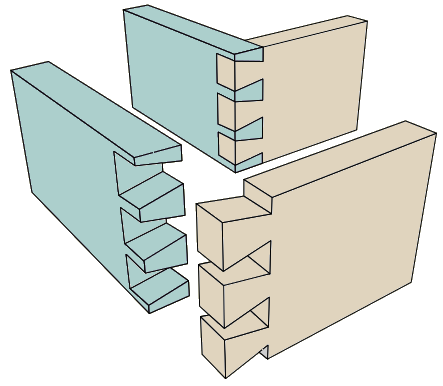
\includegraphics[width=0.15\textwidth]{background/pix/dovetail.png}
  \protect\end{center}

}。\index{dovetailing}

我们设想存在一个可计算函数 $f$，使得 $f(0)=e$，其中 $\TM_e$ 在输入 $e$ 上恰好是这些交错并行模拟中最先停机的那个，等等。
% And, $f(1)=\hat{e}$, where
% $\TM_{\hat{e}}$ on input~$\hat{e}$ is the second to halt in the dovetailing, etc.
数字流 $f(0)$、$f(1)$、\ldots{} 给出了 $K$ 的元素。

为什么这个过程解决不了停机问题呢？
如果 $e\in K$，那么交错并行最终会发现这一点。
但如果 $e\notin K$，那么它永远也无法揭示其非成员身份。

%<*def:ComputableSet>
回想一下，一个数集是可计算的\index{computable!set}\index{set!computable}% or decidable,\index{decidable!set}\index{set!decidable}，
如果其特征函数是可计算的。
%</def:ComputableSet>
我们看到了描述集合的另一种方式，% other than giving a criteria for membership,
即列出其成员。
\zcref{def:Countable} 给出了相应的术语：定义域为 $\N$ 的函数 $f$ 可“枚举”其值域。

%<*def:ComputablyEnumerable>


\begin{definition}  \label{def:ComputablyEnumerable}
一个自然数集合是
\definend{可计算枚举的}\index{computably enumerable set}\index{set!computably enumerable}\index{set!c.e.}\index{computably enumerable sets CE@computably enumerable sets \compclass{CE}}
（或 \definend{c.e.}）\@\index{c.e. set|see{computably enumerable}}，
如果它是可有效列出的，也就是说，如果它是一个可计算函数的值域。
（该函数可以是部分的。）
同义词有：
\definend{递归可枚举的}\index{recursively enumerable set|see{computably enumerable set}}\index{set!recursively enumerable|see{computably enumerable set}}\index{set!r.e.|see{computably enumerable set}}
（或 \definend{r.e.}），\@\index{r.e. set|see{computably enumerable set}}
或 \definend{半可计算的}\index{semicomputable set}\index{set!semicomputable}，
或 \definend{半可判定的}\index{semidecidable set}\index{set!semidecidable}。
由所有可计算枚举集合构成的集合记为
\citetext{$\compclass{RE}$}{%
  使用这个缩写而不是 “$\compclass{CE}$” 是因为，
  历史上“递归可枚举”曾是标准术语。}。
\end{definition}


%</def:ComputablyEnumerable>

想象由 $\TMfcn(0)$, $\TMfcn(1)$, $\TMfcn(2)$,~\ldots{} 构成的“流”逐渐填满这个集合。
（流中可能包含重复的数字，出现的顺序可能杂乱无章而不一定递增，也可能从某个点起所有的 $\TMfcn(i)$ 都发散。）

\begin{remark}
这里有一个特别有趣的“流”。
固定一个数学主题，比如初等数论。
该主题中的命题是符号串，我们可以给每个命题赋予一个编号
（例如，将该命题用 Unicode 表示，其编号即为二进制编码，并在二进制数前添加一个~\str{1}，以避免前导~\str{0} 带来的歧义）。
建立一个过程，以该主题的公理为起点，
对从这些公理出发的所有逻辑推导进行广度优先遍历。
它可能首先将公理~0 与公理~1 组合，然后将公理~0 与公理~2 组合，依此类推。
这样，它就生成了该理论所有可能证明的列表。
每当完成一个证明，该过程就输出推导中最终命题（即被证明的命题）的编号。

假设我们对这个主题中的某个命题感兴趣，
例如 \definend{Goldbach 猜想}\index{Goldbach's conjecture}（每个偶数都是至多两个素数之和）。
我们可以观察这个过程如何枚举定理。
如果该命题是可证明的，那么它的编号最终会出现。
\end{remark}

%<*lem:CEIffDomainOfComputableFcn>


\begin{lemma} \label{lem:CEIffDomainOfComputableFcn}
对于一个自然数集，下列条件等价。
\begin{thmparts}
\item 它是可计算枚举的，即它是某个可计算函数的值域。\label{itemA:lem:CEIffDomainOfComputableFcn}
\item 它是某个全可计算函数的值域，或者它是空集。\label{itemB:lem:CEIffDomainOfComputableFcn}
\item 它是某个可计算函数的定义域。
\end{thmparts}
\end{lemma}


%</lem:CEIffDomainOfComputableFcn>

\begin{proof}
我们来证明第一项和第二项等价。
第二项和第三项等价则是 \zcref{exer:CEIffDomainOfComputableFcn} 的内容。

（\ref{itemB:lem:CEIffDomainOfComputableFcn}）推（\ref{itemA:lem:CEIffDomainOfComputableFcn}）的方向是容易的。
若集合~$S$ 是某个全可计算函数的值域，那么它自然是某个可计算函数的值域。
如果 $S$ 是空集，那么它是某个永不收敛的可计算函数的值域。

现在证明（\ref{itemA:lem:CEIffDomainOfComputableFcn}）推（\ref{itemB:lem:CEIffDomainOfComputableFcn}）。
假设 $S$ 是可计算枚举的，
因此它是某个可计算函数~$\TMfcn_e$（可能不是全函数）的值域。
如果 $\TMfcn_e$ 对所有输入都发散，那么 $S=\emptyset$，这符合（\ref{itemB:lem:CEIffDomainOfComputableFcn}）中的一种情况。

另一种情况是 $\TMfcn_e$ 并非对所有输入都发散，此时我们将构造一个全可计算函数~$f$，使其值域为~$S$。
这种情况下，存在一个输入~$y$ 使得 $\TMfcn_e(y)\converges$。
令 $f(0)=\TMfcn_e(y)$。
至于函数的其他值：给定 $n\in\N$，在输入~$0$, $1$, \ldots, $n$ 上分别运行 $\TM_e$ 的计算，各运行 $n$ 步。
其中一些计算可能会停机。
设 $f(n)$ 为满足以下条件的最小 $k$：$\TM_e$ 在某个输入~$i\leq n$ 上于 $n$ 步内停机并输出~$k$，并且满足 $k\notin\set{f(0),f(1),\ldots\, f(n-1)}$。
如果不存在这样的~$k$，则令 $f(n)=s_0$。

由上一段最后一句话可知，$f$ 是全函数。
我们必须验证 $f$ 的值域就是~$S$。
对于 $t\in\N$，如果 $t\notin S$，那么 $\TM_e$ 永远不会输出它，因此 $t$ 永远不会等于某个~$f(n)$。
如果 $t\in S$，那么必然存在一个足够大的~$n$，使得 $\TM_e$ 在某个输入~$i\leq n$ 上于 $n$ 步内停机并输出~$t$。
此时，数~$t$ 就被 $f$ “排队等待输出”，这意味着它至多作为 $f(n+t)$ 被枚举出来。
\end{proof}

因此，可以有效列举的集合类，与可计算函数的定义域构成的类是相同的。
对于后者有一个标准记号。

%<*def:WSubE>


\begin{definition}
\definend{$W_e=\set{x\suchthat \TMfcn_e(x)\converges}$}
\end{definition}


%</def:WSubE>

%<*description:DecidableAndSemidecidable>
可计算集合与可计算枚举集合的区别在于：
集合~$S$ 是可计算的，如果存在一台 Turing 机能够判定其成员资格，
即输入一个数~$x$，并判定 $x\in S$ 是“是”还是“否”。
但对于可计算枚举集合，给定某个~$x$，我们可以建立一台机器来监视那个数字流，
如果 $x$ 出现，那么这台机器就判定为“是”。
然而，它可能永远也无法发现“否”。
% (Although there may well be another process that gets no's,
% as the next result notes.)
换一种说法，
一个集合是可计算的，如果存在一台 Turing 机能够同时识别成员与非成员；
而
一个集合是可计算枚举的，如果存在一台 Turing 机能够识别成员。
%</description:DecidableAndSemidecidable>

\begin{lemma}  \label{lem:ComputableAndCE}
\begin{thmparts}
\item \label{lem:SetComputableThenSetCE}
%<*lem:ComputableAndCEi>
  如果一个集合是可计算的，那么它是可计算枚举的。
%</lem:ComputableAndCEi>
\item \label{lem:SetComputableIffSetAndCompCE}
%<*lem:ComputableAndCEii>
  一个集合是可计算的，当且仅当它和它的补集都是可计算枚举的。
%</lem:ComputableAndCEii>
\end{thmparts}
\end{lemma}

\begin{proof}
对于~(\ref{lem:SetComputableThenSetCE})，令 $S\subseteq\N$ 是可计算的，因此其特征函数是一个可计算函数~$\TMfcn$。
我们将枚举~$S$ 的元素。
首先使用 $\TMfcn$ 来检验 $0\in S$ 是否成立，即 $\TMfcn(0)=1$ 是否成立。
然后检验 $1\in S$ 是否成立，以此类推。
如果这一系列检验最终找到某个 $k_0$ 使得 $\TMfcn(k_0)=1$，
则令 $f(0)=k_0$。
之后，迭代进行：通过检验 $k_0+1\in S$、 $k_0+2\in S$、\ldots{} 来寻找 $S$ 的下一个元素，
如果这一系列检验最终找到某个 $k_1$，则令 $f(1)=k_1$。
显然~$f$ 是一个值域为~$S$ 的可计算函数。

至于 (\ref{lem:SetComputableIffSetAndCompCE})，
首先假设 $S$ 是可计算的。
其补集 $\setcomp{S}$ 也是可计算的，因为
$\charfcn{\setcomp{S}}(x)=1-\charfcn{S}(x)$ 对所有~$x$ 成立。
由此，根据第~(\ref{lem:SetComputableThenSetCE}) 项，$S$ 和 $\setcomp{S}$ 都是可计算枚举的。

反之，
假设 $S$ 和 $\setcomp{S}$ 都是可计算枚举的。
设 $S$ 由函数~$g$ 枚举，$\setcomp{S}$ 由 $\hat{g}$ 枚举。
为证明 $S$ 是可计算的，我们将给出一个有效过程，它充当 $S$ 的特征过程，也就是说，给定~$x\in\N$，该过程能判定~$x\in S$ 是否成立。
思路是交错并行这两个枚举：首先让 $g(0)$ 的计算运行一步，同时让 $\hat{g}(0)$ 的计算也运行一步。
接下来，让 $g(0)$ 和 $\hat{g}(0)$ 的计算各进行第二步，同时让 $g(1)$ 和 $\hat{g}(1)$ 的计算各进行一步。
以这种方式继续下去，
最终我们将发现 $x$ 被枚举进入了 $S$ 或~$\setcomp{S}\!$ 中的一个。
\end{proof}

%<*lem:HPIsCE>


\begin{corollary} \label{cor:KCompNotCE}
\HP{} 集 $K$ 是可计算枚举的。\index{K, the Halting problem set@$K$, the Halting problem set}
其补集 $\setcomp{K}$ 则不是。
\end{corollary}


%</lem:HPIsCE>

\begin{proof}
集合~$K$ 是
$f(x)=\TMfcn_x(x)$
的定义域，
根据 Church 论题，这是一个偏可计算函数。
所以 $K$ 是可计算枚举的。
如果补集~$\setcomp{K}$ 也是可计算枚举的，那么
\zcref{lem:ComputableAndCE} 将推出 $K$ 是可计算的，
但事实并非如此。
\end{proof}

这个结果给出了关注可计算枚举集的一个理由，即
\HP{} 集~$K$ 属于这类集合，
像集合
$\set{e\suchthat \TMfcn_e(3)\converges}$
和 $\set{e\suchthat \text{there is an $x$ so that $\TMfcn_e(x)=7$}}$ 也是如此。
所以，可计算枚举集构成的类包含了许多有趣的成员。

这些集合令人感兴趣的另一个原因是哲学上的：考虑到 Church 论题，我们可以意识到，在某种意义上，可计算集是我们能够完全了解的唯一一类集合。
与这种认识相一致，可计算枚举集正是我们至少拥有部分信息的集合：我们能判定哪些元素在其中，但未必能判定哪些元素不在其中。

% .......................................
\begin{exercises}
\recommended


\begin{exercise}
一次小测上有一道题要求你定义“可计算枚举”。
一位朋友说他回答的是：
“一个可以由 Turing 机枚举，但不是可计算的集合。”
这回答正确吗？
\begin{answer}\verified
 只对了一半。
 若一个集合能被 Turing 机枚举就是可计算枚举的，这是对的。
 但“不是可计算的”是错的。
 例如，偶数集是可计算枚举的，因为它显然可以有效列举，同时它也是可计算的，因为其特征函数是可计算的。
\end{answer}
\end{exercise}

\begin{exercise}
你的学伴问大家：“空集是一个可计算枚举集。
但空集不是有效列举的，因为你没法列举‘没有东西’。”
他/她的思路哪里出了岔子？
\begin{answer}\verified
“有效列举”的意思是，某个机器过程将其作为输出集合给出。
有些 Turing 机无论输入什么都不会停机，
这些机器所枚举的就是空集。
\end{answer}
\end{exercise}

\recommended


\begin{exercise}
对于每一小问，构造一个能枚举它的函数。
\begin{exparts*}
\item $\N$
\item 偶数集
\item 完全平方数集
\item 集合 $\set{5,7,11}$。
\end{exparts*}
\begin{answer}\verified
对于每一小问，我们将给出一个可计算的全函数 $\map{f}{\N}{\N}$，使其值域为给定集合。
\begin{exparts}
  \item 恒等函数 $f(x)=x$ 即可。
  \item 函数 $f(x)=2x$ 即可。
  \item $f(x)=x^2$
  \item 这个函数可行。
  \begin{equation*}
     f(x)=
     \begin{cases}
       5  &\case{if $x=0$}  \\
       7  &\case{if $x=1$}  \\
      11  &\case{otherwise}
     \end{cases}
  \end{equation*}
  \end{exparts}
\end{answer}
\end{exercise}

\begin{exercise}
对以下各项，分别构造一个枚举它们的函数
\begin{exparts*}
\item 素数
\item 各位数字非递增的自然数
  （例如 $531$ 或 $5331$，但 $513$ 不符合）。
\end{exparts*}
\begin{answer}\verified
  对每一项，我们构造一个有效函数 $\map{f}{\N}{\N}$。
  \begin{exparts}
  \item 对应关系 $n\mapsto\text{$n$-th prime}$ 是一个函数。
    显然我们可以编写一个程序来计算它，因此由 Church 论题可知它是有效的。
  \item 为了计算这个函数，我们可以采用暴力搜索：给定~$n$，
    遍历自然数 $0$, $1$, \ldots{}\,，检查每个数的各位数字是否按非递增顺序出现，
    输出第 $n$ 个这样的数。
  \end{exparts}
\end{answer}
\end{exercise}

\begin{exercise}
是否存在无限的可计算枚举集？
有限的呢？
空集呢？
所有自然数的集合呢？
\begin{answer}\verified
以上四种情况都存在。
对于第一种和第四种情况，
我们可以编写一台 Turing 机，其输入/输出行为即为恒等函数 $x\mapsto x$，
这台机器枚举了所有的自然数。
因此，所有自然数的集合是可计算枚举的。

对于第二种和第三种情况，存在在任何输入上都不停机的 Turing 机，
所以空集是可计算枚举的。
\end{answer}
\end{exercise}

\begin{exercise}
以下两个集合中，一个是可计算的，另一个是可计算枚举但不可计算的。
哪个是哪个？
\begin{exparts}
\item $\set{e\suchthat \text{$\TM_e$ halts on input~$4$ in less than twenty steps}}$
\item $\set{e\suchthat \text{$\TM_e$ halts on input~$4$ in more than twenty steps}}$
\end{exparts}
\begin{answer}\verified
  第一个是可计算的，因为要判定一个数~$e$ 是否属于这个集合，我们只需要模拟二十步。
  第二个是可计算枚举但不可计算的。
  它是可计算枚举的，因为我们可以对索引 $e\in\N$ 进行交错并行计算。
  它是不可计算的，因为显然如果我们能解决它，我们就能解决判定 $\set{e\suchthat \TMfcn_e(4)\converges}$ 的成员归属问题，但由 Rice 定理可知我们无法解决那个问题。
\end{answer}
\end{exercise}

\begin{exercise}
下列集合哪些是可判定的，哪些是半可判定但不可判定的，哪些两者都不是？
用一句话论证。
\begin{exparts*}
\item
索引~$e$ 的集合，其中 $\TM_e$ 在输入~$7$ 上的运行步骤超过 $100$。
\item
索引~$e$ 的集合，其中 $\TM_e$ 在输入~$7$ 上的运行步骤少于 $100$。
\end{exparts*}
\begin{answer}\verified
对于集合来说，“可判定的”与“可计算的”含义相同，即其特征函数是全可计算函数。
同时，“半可判定的”与“可计算枚举的”含义相同。
\begin{exparts}
\item
这个集合是可计算的，因为我们只需要运行机器一百步。
由于它是可计算的，所以它也是可计算枚举的。
\item
这个集合也是可计算的，同样因为我们只需要运行机器一百步。
由于它是可计算的，所以它也是可计算枚举的。
\end{exparts}
\end{answer}
\end{exercise}

\begin{exercise} \autocite{GATE22}
以下两个陈述中，有一个是真的。
是哪一个？
\begin{exparts*}
\item 任何可计算枚举集的真子集都是可计算的。
\item 如果一个集合及其补集都是可计算枚举的，那么两者都是可计算的。
\end{exparts*}
\begin{answer}\verified
第二个陈述为真，由引理 \zcref{lem:ComputableAndCE} 即得。
第一个陈述为假；例如，集合~$\N$ 是可计算枚举的，
但其真子集 $K$ 不是可计算的。
\end{answer}
\end{exercise}

\recommended


\begin{exercise}
网上有人说，
“每个可数集~$S$ 都是可计算枚举的，因为如果 $\map{f}{\N}{\N}$ 的值域是~$S$，那么你就有了 $S$ 的枚举，即 $f(0)$, $f(1)$, \ldots”\sentencespace
解释为什么这是错的。
\begin{answer}\verified
  这个函数确实是一个枚举，但除非它是可计算的，否则这就不是可计算枚举。
  一个可数但不可计算枚举的集合的例子是 $\setcomp{K}\!$。
  它是可数的，因为它是可数集~$\N$ 的一个子集，
  并且由推论 \zcref{cor:KCompNotCE} 可知它是不可计算枚举的。
\end{answer}
\end{exercise}

\recommended


\begin{exercise}
集合 $A_5=\set{e\suchthat \TMfcn_e(5)\converges}$ 是不可计算的。
证明它是可计算枚举的。
\begin{answer}\verified
  简言之，我们采用交错并行。
  为了得到枚举，首先在输入~$5$ 上运行 $\TM_0$ 一步。
  然后在输入~$5$ 上运行 $\TM_0$ 第二步，同时运行 $\TM_1$ 一步。
  接着在输入~$5$ 上运行 $\TM_0$ 第三步，同时运行 $\TM_1$ 第二步以及 $\TM_2$ 一步。
  依此方式继续。
  枚举函数~$\map{f}{\N}{\N}$ 定义为：~$f(0)$ 是第一个停机的这类计算的索引，$f(1)$ 是第二个，依此类推。
\end{answer}
\end{exercise}

\begin{exercise}
证明可计算枚举集的全体是可数的。
\begin{answer}\verified
因为用来执行枚举的 Turing 机只有可数多台。
\end{answer}
\end{exercise}

\begin{exercise}
每个不可计算集都是无限的，
因为每个有限集都是可计算的。
那么，每个可计算枚举集都是无限的吗？
\begin{answer}\verified
不是。
空集是可计算枚举的，但是有限的。
\end{answer}
\end{exercise}

\begin{exercise}
简答题：对于每个集合，判断它是可计算的、可计算枚举但不可计算的，还是两者皆非。
\begin{exparts*}
\item 包含以状态~$q_4$ 开头的指令的 Turing 机的索引~$e$ 所构成的集合。
\item 在输入~$4$ 上停机的 Turing 机的索引构成的集合。
\item 在输入~$4$ 上于少于 $100$ 步内停机的 Turing 机的索引所构成的集合。
\end{exparts*}
\begin{answer}\verified
  \begin{exparts}
  \item 该集合是可计算的。
  给定一个索引~$e$，我们需要判定 $\TM_e$ 是否包含这样的指令。
  索引与源码等价，这意味着存在一个程序，输入索引~$e$ 即可输出~$\TM_e$ 的指令集。
  然后我们可以通过扫描指令集中是否有以~$q_4$ 开头的指令，来判定 $e$ 是否属于该集合。
  \item 该集合是可计算枚举但不可计算的。
  要证明它是可计算枚举的，可以对索引~$e\in\N$ 使用交错并行方法，在输入~$4$ 上运行各台 $\TM_e$。
  也就是说，先在输入~$4$ 上运行 $\TM_0$ 一步。
  接着，在输入~$4$ 上再运行 $\TM_0$ 一步，同时在输入~$4$ 上运行 $\TM_1$ 一步。
  继续这个过程，当一个计算停机时，就将其索引~$e$ 枚举入集合。
  至于该集合不可计算，由 Rice 定理很容易得出它不是可计算集。
  \item 可计算的。
  给定~$e$，通过在输入~$4$ 上运行~$\TM_e$ 一百步来判定它是否属于该集合。
  \end{exparts}
\end{answer}
\end{exercise}

\begin{exercise}
证明集合
$\set{e\suchthat \TMfcn_e(2)=4}$
是可计算枚举的。
\begin{answer}\verified
  要枚举它，采用交错并行方法。
  首先在输入~$2$ 上运行 $\TM_0$ 一步。
  然后在输入~$2$ 上运行 $\TM_0$ 第二步，同时运行 $\TM_1$ 一步。
  接着，运行 $\TM_0$ 第三步，$\TM_1$ 第二步，以及 $\TM_2$ 一步。
  以此类推，继续这个过程。
  令~$f(0)$ 为第一个停机并输出~$4$ 的计算的索引，
  令 $f(1)$ 为第二个这样的索引，等等。
\end{answer}
\end{exercise}

\begin{exercise}
列举三个可计算枚举但不可计算的集合。
\begin{answer}\verified
  当然有很多正确答案。
  一个答案是取~$K$ 作为第一个集合。
  第二个集合取去掉最小元素的~$K$，
  第三个集合取去掉最小的两个元素的~$K$。

  一个或许不那么取巧的答案是取~$K$ 再加上前两节中用过的一些集合作为例子，例如
  $\set{e\in\N\suchthat \TMfcn_e(3)\converges}$
  和 $\set{e\in\N\suchthat \text{there is $x\in\N$ so that $\TMfcn_e(x)=7$}}$。
  后两者可通过交错并行过程证明是可计算枚举的。
\end{answer}
\end{exercise}

\recommended

\begin{exercise}
令 $K_0=\set{\sequence{e,x}\suchthat \text{$\TM_e$ halts on input $x$}}$。\index{K0, set of halting pairs@$K_0$, set of halting pairs}
\begin{exparts*}
\item
证明它是可计算枚举的。
\item
证明它的列，即集合 $C_e=\set{\sequence{e,x}\suchthat \text{$\TM_e$ halts on input $x$}}$，构成了所有的可计算枚举集。
\end{exparts*}
\begin{answer}\verified
  \begin{exparts}
  \item
  通过交错并行来枚举它。
  与之前一些交错并行的例子不同的是，这里有两个数，$e$ 和~$x$。
  因此回顾 Cantor 配对函数。
  \begin{center}
    \begin{tabular}{r|ccccccc@{\hspace{6pt}}c}
      \tabulartext{数}
         &$0$    &$1$   &$2$  &$3$  &$4$  &$5$  &$6$ &\ldots
     \\ \cline{2-9}
      \tabulartext{对}
                 &$\sequence{0,0}$
                 &$\sequence{0,1}$
                 &$\sequence{1,0}$
                 &$\sequence{0,2}$
                 &$\sequence{1,1}$
                 &$\sequence{2,0}$
                 &$\sequence{0,3}$
                 &\ldots
       \end{tabular}
  \end{center}
  在交错并行循环的第一次迭代中，找到表格中的第一个对 $\sequence{0,0}$（我们将第一个数视为~$e$，第二个视为~$x$），并以 $0$ 为输入运行 $\TM_0$ 执行一步。
  在循环的第二次迭代中，以 $0$ 为输入运行 $\TM_0$ 执行第二步，并且同时运行（因为 $\sequence{0,1}$ 是第二个对）$\TM_0$ 以 $1$ 为输入执行一步。
  在第三次迭代中，以 $0$ 为输入运行 $\TM_0$ 执行其第三步，以 $1$ 为输入运行 $\TM_0$ 执行第二步，以及以 $0$ 为输入运行 $\TM_1$ 执行一步。
  当 $\TM_e$ 在输入 $x$ 上停机时，枚举函数输出 $\sequence{e,x}$。
  \item
  这可以直接从 \zcref{lem:CEIffDomainOfComputableFcn} 得出。
  \end{exparts}
\end{answer}
\end{exercise}

\begin{exercise}
我们知道存在~$\N$ 的不可计算子集。
可计算枚举集是否就是那些不可计算的子集呢？
\begin{answer}\verified
  否，原因有二。

  首先，可计算集类与可计算枚举集类并非不相交。
  实际上，由 \zcref{lem:ComputableAndCE}，可计算集类是可计算枚举集类的一个子集。

  此外，集合 $\set{W_e\suchthat e\in\N}$ 是可数的，因为该集合中的元素，即各个 $W_e$，是由自然数索引的。
  由于~$\N$ 的子集个数是不可数的（因为~$\N$ 的幂集的势大于~$\N$），所以~$\N$ 的子集比可计算枚举集要多。
  因此，存在 $\N$ 的子集不是可计算枚举的。
\end{answer}
\end{exercise}

\recommended


\begin{exercise}
证明集合 $\text{Tot}=\set{e\suchthat \text{$\TMfcn_e(x)\converges$ for all $x$}}$\index{Tot@$\text{Tot}$, set of total computable functions}
不可计算且不可计算枚举。
\hint~如果这个集合是可计算枚举的，那么我们可以得到一个类似于第~II.\ref{sec:HaltingProblem}节开头关于\HP 的表格。
\begin{answer}\verified
  可计算集也是可计算枚举的，所以只要我们证明了 $\textrm{Tot}$ 不是可计算枚举的，也就证明了它既不可计算也不可计算枚举。

  反设 $\text{Tot}=\set{e\suchthat \text{$\TMfcn_e(x)\converges$ for all $x$}}$ 是可计算枚举的，并由函数~$\map{f}{\N}{\N}$ 枚举。
  根据提示，这给出了一个类似于 \zcref{sec:HaltingProblem} 中关于\HP 的表格，因为第 $i,j$ 项 $\TMfcn_{f(i)}(j)$ 必定停机。
  对角化：考虑由 $h(i)=1+\TMfcn_{f(i)}(i)$ 给出的函数 $\map{h}{\N}{\N}$。
  该函数是有效的、全函数，且与 $\textrm{Tot}$ 中的任何成员都不相等，矛盾。
\end{answer}
\end{exercise}

\begin{exercise}
证明集合 $\set{e\suchthat \TMfcn_e(3)\diverges}$ 不是可计算枚举的。
\begin{answer}\verified
  由 Rice 定理容易证明集合 $S=\set{e\suchthat \TMfcn_e(3)\diverges}$ 不可计算。
  显然，其补集 $\setcomp{S}=\set{e\suchthat \TMfcn_e(3)\converges}$ 是可计算枚举的\Dash 只需使用交错并行，并在元素收敛时枚举它们。
  如果 $S$ 也是可计算枚举的，那么由 \zcref{lem:ComputableAndCE}，它将是可计算的，矛盾。
\end{answer}
\end{exercise}

% \begin{exercise}
% Can there be a set such that the problem of determining membership in that
% set is unsolvable, and also the set is computably enumerable?
% \begin{answer}\verified
%   Yes, the \HP{} set~$K$ fits both criteria.
%   Three other examples are the set
%   $\set{e\in\N\suchthat \TMfcn_e(3)\converges}$,
%   the set
%   $\set{e\in\N\suchthat \text{there is $x\in\N$ so that $\TMfcn_e(x)=7$}}$,
%   and $\set{e\in\N\suchthat\text{$\TMfcn_e(x)=2x$ for all $x\in\N$}}$.
% \end{answer}
% \end{exercise}

% \begin{exercise}
% \begin{exparts*}
% \item
% Prove that every finite set is computably enumerable.
% \item
% Sketch a program that inputs a finite set and returns
% a function enumerating the set.
% \end{exparts*}
% \begin{answer}\verified
%   The answer to the second effectively answers the first, but we will do both
%   items anyway.
%   \begin{exparts}
%   \item
%   Let $S=\set{s_0,\ldots s_{k-1}}$ for~$k\in\N$.
%   Then this function enumerates~$S$.
%   \begin{equation*}
%     f(x)=
%     \begin{cases}
%       1  &\case{if $x=s_0$ or \ldots{} or $x=s_{k-1}$}  \\
%       0  &\case{otherwise}
%     \end{cases}
%   \end{equation*}
%   It is clearly computable.
%   \item
%   The algorithm inputs a set of numbers $S=\set{s_0,\ldots s_{k-1}}$.
%   It returns a function, the one in the prior item.
%   This function is clearly computable.

%   Another approach is to start with the number $k=\sizeof{S}$.
%   Define a function with  $k+1$ inputs, $x_0,\ldots x_{k-1},y$ that
%   tests whether $y$ equals any of the $x_i$'s, and returns~$1$ if
%   it does or~$0$ if it does not.
%   Where $S=\set{s_0,\ldots s_{k-1}}$, apply the \smn{} Theorem to freeze
%   the value of each $x_i$ to be~$s_i$.
%   That's the desired function.
%   \end{exparts}
% \end{answer}
% \end{exercise}

\recommended


\begin{exercise}
证明每个无限的可计算枚举集都有一个无限的可计算子集。
\begin{answer}\verified
  设该无限的可计算枚举集为 $W$，并固定一个可计算枚举 $\TMfcn(0)$, $\TMfcn(1)$, \ldots\sentencespace
  我们将定义一个无限的可计算子集 $S\subseteq W$。

  令 $S$ 的第一个元素为~$s_0=\TMfcn(0)$。
  取第二个元素~$s_1$ 为枚举中第一个大于 $s_0$ 的数；由于 $W$ 是无限的，这样的数终将出现。
  一般地，令 $s_{i+1}$ 为枚举中第一个大于 $s_{i}$ 的元素（与 $s_1$ 的情况一样，由于 $W$ 无限，这样的元素终将出现）。

  集合~$S$ 是可计算枚举的，因为我们刚才描述了一个枚举它的机械过程。
  它是可计算的，因为给定一个数 $n\in\N$，要判定它是否属于 $S$，只需等待，直到它被枚举进 $S$，或者有一个比它大的数被枚举进 $S$（这表明 $n\notin S$）。
\end{answer}
\end{exercise}

\begin{exercise}
定义函数 $\operatorname{steps}$ 如下：
$\operatorname{steps}(e)$ 是 Turing 机 $\TM_e$ 以 $e$ 为输入启动后停机所需的最少步数，若机器永不停机则无定义。
\begin{exparts*}
\item 论证此函数是部分可计算的。
\item 论证它不是全函数。
\item 证明它没有全可计算的延拓，即不存在全可计算函数 $\map{f}{\N}{\N}$，使得若 $\operatorname{steps}(e)\converges$ 则
$\operatorname{steps}(e)=f(e)$。
\end{exparts*}
\begin{answer}\verified
\begin{exparts}
\item 我们可以根据 Church 论题来论证：以 $e$ 为输入运行 $\TM_e$（使用一台通用 Turing 机）来计算 $\operatorname{steps}(e)$，若它停机，则输出步数。
\item
我们断言，如果 $\operatorname{steps}$ 既是可计算的又是全函数，那么我们就能解决停机问题 \HP。
原因是，要判定 $e\in K$，首先计算 $\operatorname{steps}(e)$。
然后以 $e$ 为输入运行 $\TM_e$ 共 $\operatorname{steps}(e)$ 步。
若此计算在那 $\operatorname{steps}(e)$ 步之后仍未停机，则它将永不停机。
\item
这与前面的论证相同，只是用~$f$ 代替了 $\operatorname{steps}$。
\end{exparts}
\end{answer}
\end{exercise}

% \begin{exercise}
% Suppose that there is a set $A$ and a computable function $f$ such that
% the set difference $A-\operatorname{range}(f)$ is finite.
% Show that $A$ is computably enumerable.
% \end{exercise}

% \begin{exercise}
% Write a program that will, given two enumerating programs, dovetail them.
% \end{exercise}

\begin{exercise}
一个集合是 \definend{按严格递增次序可计算枚举的（computably enumerable in increasing order）}\index{computably enumerable set!enumerated in increasing order}，如果存在一个递增的可计算函数 $f$（即 $n<m$ 蕴含 $f(n)<f(m)$），且其值域恰好为该集合。
假设集合 $S$ 是无限的。
证明 $S$ 是可计算的当且仅当它是按严格递增次序可计算枚举的。
\begin{answer}\verified
  假设 $S$ 是可计算的，那么其特征函数
  \begin{equation*}
    \charfcn{S}(x)=
    \begin{cases}
      1  &\case{if $x\in S$}  \\
      0  &\case{if not}
    \end{cases}
  \end{equation*}
  是一个可计算函数。
  为了按严格递增次序枚举 $S$，运行 $\charfcn{S}(0)$, $\charfcn{S}(1)$, \ldots{}\,，由于函数是可计算的，它们必然都会收敛，那么 $S$ 的第一个元素是最小的，第二个元素是第二小的，等等。

  更形式化地说，定义枚举函数如下：设 $s_0$ 是 $S$ 的最小元素，则 $f(0)=s_0$；若我们已得到 $f(0)$, \ldots{} $f(k)$ 的值，则 $f(k+1)$ 是满足 $x>f(k)$ 且 $\charfcn{S}(x)=1$ 的最小 $x$。
  因为 $S$ 是无限的，总存在这样的 $x$。

  反之，假设 $S$ 是一个可由可计算函数 $h$ 按严格递增次序枚举的无限集。
  给定 $x$，要判定 $x\in S$，计算 $h(0)$, $h(1)$, \ldots{} 直到输出为 $x$（于是 $x\in S$）或者输出大于 $x$（于是 $x\notin S$）。
\end{answer}
\end{exercise}

% \begin{exercise}
% A set is
% \definend{computably enumerable without repetition}\index{computably enumerable set!without repetition} if it is
% the range of a computable function that is one-to-one.
% Prove that a set is computably enumerable and infinite if and only if
% it is computably enumerable without repetition.
% \begin{answer}\verified
% One direction is easy.
% If a set is computably enumerable without repetition then
% it must be infinite, simply because if it were finite then
% the enumeration would run out of new elements to output.

% The other direction is about memoizing.
% Let the set~$S$ be infinite and computably enumerable with
% enumerating function $f$.
% We will produce an enumerating function~$g$ that is one-to-one.
% Define $g(0)=f(0)$.
% For each $i\in\N$ define $g(i+1)$ to be the first element of~$S$ enumerated
% by~$f$ after it enumerates~$g(i)$ that is not an element
% of~$\set{g(0),\ldots\, g(i)}$.
% \end{answer}
% \end{exercise}

\begin{exercise}
一个集合是 \definend{余可计算枚举的（co-computably enumerable）}\index{computably enumerable set!co-computably enumerable}\index{co-computably enumerable}，如果它的补集是可计算枚举的。
构造一个既不可计算枚举也不余可计算枚举的集合。
\begin{answer}\verified
  考虑序对集合
  $S=\set{\sequence{a,b}\suchthat
       \text{$a\in K$ and $b\in\setcomp{K}$}}$。
  它不是可计算枚举的，否则枚举它将枚举其第二分量，但 $\setcomp{K}$ 不是可计算枚举的。
  类似地，它的补集也不是可计算枚举的，否则枚举它将枚举 $S$ 的第一分量集合的补集，这同样不可能，因为 $\setcomp{K}$ 不是可计算枚举的。
\end{answer}
\end{exercise}

\begin{exercise}\textit{（与下一练习对比。）}
可计算性是集合的一个性质，因此我们可以考察它与集合运算的交互。
\begin{exparts*}
\item
可计算集合的子集一定可计算吗？
\item
两个可计算集合的并集一定可计算吗？
\item
交集呢？
\item
补集呢？
\end{exparts*}
\begin{answer}\verified
  \begin{figure}
    \centering
    \vcenteredhbox{\includegraphics{\asydir hp/hp1024.pdf}}
    \qquad
    \vcenteredhbox{\includegraphics{\asydir hp/hp1025.pdf}}
    \qquad
    \vcenteredhbox{\includegraphics{\asydir hp/hp1026.pdf}}
    \caption{可计算集合的并、交、补的判定机草图。}
    \label{fig:ComputableSetsUnionInt}
  \end{figure}
  \begin{exparts}
  \item 否。
  集合 $\N$ 是可计算的，但其子集~$K$ 不可计算。
  \item 是。
  设 $S_0\subseteq \N$ 和 $S_1\subseteq\N$ 分别通过函数 $\TMfcn_{e_0}$ 和~$\TMfcn_{e_1}$ 可计算。
  计算并集的机器草图见 \figureref{fig:ComputableSetsUnionInt}。
  \item 是。
  计算交集的机器草图也在同一图中。
  \item 是。
  计算补集的机器草图也在该图中。
  \end{exparts}
\end{answer}
\end{exercise}

\begin{exercise}\textit{（与前一练习对比。）}
我们可以考察可计算枚举性与集合运算的交互。
\begin{exparts*}
\item
可计算枚举集合的子集一定是可计算枚举的吗？
\item
两个可计算枚举集合的并集一定是可计算枚举的吗？
\item
交集呢？
\item
补集呢？
\end{exparts*}
\begin{answer}\verified
  \begin{exparts}
  \item 否。
  集合~$\N$ 是可计算枚举的。
  停机问题集的补集 $\setcomp{K}\!$ 是 $\N$ 的子集，并且不是可计算枚举的。
  \item 是。
  设 $W_{e_0},W_{e_1}\subseteq\N$ 是可计算枚举的，
  分别通过 $\map{\TMfcn_{e_0},\TMfcn_{e_1}}{\N}{\N}$ 枚举。
  对这两个集合进行交错并行枚举。
  也就是说，先让 $\TM_{e_0}$ 和~$\TM_{e_1}$ 在输入~$0$ 上各运行一步。
  然后，让 $\TM_{e_0}$ 和~$\TM_{e_1}$ 在输入~$0$ 上再运行一步，
  同时让它们在输入~$1$ 上各运行一步。
  如此继续，当某个数被枚举进 $W_{e_0}$ 或~$W_{e_1}$ 时，
  就将其枚举进它们的并集。
  \item 是。
  如上一项所述，对这两个集合进行交错并行枚举。
  当某个数已被同时枚举进 $W_{e_0}$ 和~$W_{e_1}$ 时，
  再将其枚举进它们的交集。
  \item 否。
  停机问题集~$K$ 是可计算枚举的，但其补集不是。
  \end{exparts}
\end{answer}
\end{exercise}

% \begin{exercise}
% Show that if $h$ is a partially computable function and
% $S$ is a computably enumerable set, then the inverse image
% $h^{-1}(S)$ is computably enumerable.
% \end{exercise}

% \begin{exercise}
% A set $S\subseteq \N^k$ is a \textit{projection}
% of the set $T\subseteq\N^{k+1}$
% if $S$ is the set of $k$-tuples $\sequence{x_0,\ldots x_{k-1}}$ such that
% there is a $i\in\N$ so that $\sequence{i,x_0,\ldots x_{k-1}}\in T$.
% Prove that the projection of a computably enumerable set is also
% computably enumerable.
% \end{exercise}

\begin{exercise}  \label{exer:CEIffDomainOfComputableFcn}
通过证明第二项和第三项等价，完成 \zcref{lem:CEIffDomainOfComputableFcn} 的证明。
\begin{answer}\verified
我们必须证明：如果集合~$S$ 是全可计算函数的值域或是空集，那么 $S$ 是某个部分可计算函数的定义域。

我们先证从左到右的蕴含。
若 $S$ 为空集，
则它是处处发散的部分可计算函数的定义域。
否则 $S$ 是全可计算函数~$f$ 的值域；我们将描述一个定义域为~$S$ 的部分可计算函数~$g$。
计算 $g$ 的方法如下：给定输入~$x\in\N$，
枚举 $f(0)$, $f(1)$, \ldots\sentencespace
如果~$x$ 出现在这个序列中，则停止对~$g$ 的计算（并输出某个任意值）。
如果~$x$ 从未出现，则 $g(x)$ 的计算永不停机。
这样，$g$ 的定义域就是~$S$。

对于另一个方向的蕴含，
假设 $S$ 是某个部分可计算函数~$\hat{g}$ 的定义域。
我们必须证明 $S$ 要么是空集，要么是某个全可计算函数的值域。
部分可计算函数的定义域可以是空集；如果 $S$ 是空集，则结论成立。
否则固定某个 $s_0\in S$，
我们将构造一个值域为~$S$ 的全可计算函数~$\hat{f}$。
给定 $n\in \N$，执行
$\hat{g}(0)$, $\hat{g}(1)$, \ldots{} $\hat{g}(n)$ 的计算，每个各运行 $n$ 步。
其中某些计算可能会停机。
定义 $\hat{f}(n)$ 为满足以下条件的、最小的 $k$：$\hat{g}(k)$ 的计算在~$n$ 步内停机，且
$k\notin\set{\hat{f}(0),\hat{f}(1),\ldots\, \hat{f}(n-1)}$。
如果不存在这样的~$k$，则定义 $\hat{f}(n)=s_0$（这保证了 $\hat{f}$ 是全函数）。

最后验证 $\hat{f}$ 确实是所需的枚举。
若 $t\notin S$，则 $\hat{g}(t)$ 的计算永不停机，
因此~$t$ 永远不会被~$\hat{f}$ 枚举。
若 $t\in S$，则 $\hat{g}(t)$ 的计算最终必在若干步（设为 $n_t$）后停机。
于是数~$t$ 被列入~$\hat{f}$ 的输出队列，它至多在 $\hat{f}(n_t+t)$ 时被枚举。
\end{answer}
\end{exercise}

\end{exercises}
\index{computably enumerable|)}\index{set!computably enumerable|)}

\section{预言机}\index{oracle|(}\index{set!oracle|(} \label{sec:Oracles}
\margingraphic{0.20\textwidth}{background/pix/delphi.jpg}{\label{fig:yogi}\href{https://en.wikipedia.org/wiki/Oracle}{Priestess of Delphi (Collier 1891)}}
判定一台给定机器是否停机的问题难到不可解。
这就是绝对最难的问题了吗，还是存在更难的问题？

% \margingraphic{0.23\textwidth}{background/pix/delphi.png}{\label{fig:yogi}\href{https://en.wikipedia.org/wiki/Pythia}{The oracle at Delphi}}
要回答这个问题，我们必须先定义“一个问题比另一个问题难”是什么意思。
其实我们已经比较过问题的难度了，
例如之前我们考虑过“Turing 机在输入~$3$ 上是否停机”这个问题。
当时我们证明了，如果能解决“在输入3上停机”问题，那么我们就能解决停机问题（\HP）。
也就是说，我们证明了“在输入3上停机”问题至少和停机问题一样难。
因此，其核心思想是：
如果解决第一个问题也能给出第二个问题的解，那么第一个问题至少和第二个问题一样难。\footnote{%
  我们也可以从另一个角度理解：第一个问题至少和第二个问题一样一般。
  举个例子：输入一个自然数并输出其质因数的问题，至少和输入一个自然数并判断它是否能被七整除的问题一样一般。}

根据 Church 论题，我们将停机问题（\HP）的不可解性解读为：
没有任何机制能回答所有关于~$K$ 中成员资格的问题。
因此，如果我们想回答与~$K$ 相关的问题，
就需要这些答案以某种在原则上并非物理可实现的离散机器的方式来提供。\footnote{%
  Turing 在其博士论文中引入了预言机。
  他说：\protect\citetext{“我们不再深入探究这个预言机的本质，
  除了说它不可能是一台机器。”}{%
  \autocite{TuringThesis}}}

于是，我们设定一个
\definend{预言机（oracle）}\index{oracle!background}，
把它附加到 Turing 机上，让它充当某个集合的特征函数。
这样，为了看看如果我们以某种方式解决了停机问题（\HP）能够计算什么，
我们就附加一个 $K$ 预言机，让它回答形如“$x\in K$吗？”的问题。
这个预言机是一个黑盒，意思是
\citetext{我们不能打开它看它是如何工作的}{%
  打开它会让魔法烟雾（参见 \autocite{wiki:MagicSmoke}）跑出来，
  那是电子元件内部让它工作的东西。
  烟雾一旦跑出来，元件就不再工作了。}。

\begin{center}
  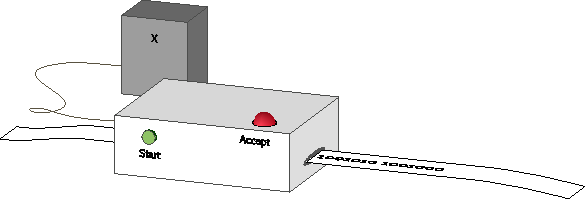
\includegraphics{asy/share/machine01.pdf}
\end{center}

我们可以通过扩展 Turing 机的定义，来形式化地定义
\definend{相对于预言机的计算（computation relative to an oracle）}\index{computation!relative to an oracle}\index{oracle!computation relative to}
$X\subseteq\N$。
不过，本节中底层细节的帮助不大，所以
\citetext{我们将在概念上描述它}{%
  完整的处理请见 \autocite{Rogers}.}。
想象一下，从一个编程语言出发，添加一个布尔函数 \codeinline{oracle?}，
或者允许流程图包含查询步骤。\footnote{%
  一次相对于预言机的特定计算，可能会使用一次这样的查询，或多次，或一次也不用。
  }


\begin{center}
\begin{minipage}{2.3in}
\begin{lstlisting}
(if (oracle? x)
    (displayln "It is in the set")
    (displayln "It is not in the set"))
\end{lstlisting}
\end{minipage}
\qquad
\vcenteredhbox{\includegraphics{\asydir flowcharts/flowcharts21.pdf}}
\end{center}


% If $x\in X$
% then this takes one branch, while if $x\notin X$ then it takes the other.

我们可以更换预言机而不改变程序代码：
在图中，如果我们换掉黑盒，把 $X$~预言机换成 $Y$~预言机，
那么白色的 CPU 盒保持不变。
当然，预言机查询返回的值可能会改变，
从而可能在我们运行这个双盒系统时改变纸带输出。
但这样的交换不会改变白色的硬件。

我们已有的关于 Turing 机的其他结论同样适用。
特别地，每一台这样的机器——每一个 CPU 盒——都有一个索引。
这个索引是源码等价的，意思是给定一个索引，我们可以计算出
机器的源代码，而给定源代码，我们可以找到索引。

因此，要完整地指定这样一个计算，我们必须同时指明
我们使用的是哪台机器以及哪个预言机。
这就解释了带预言机的 Turing 机的记号：
\definend{$\TM_e^X\!$}，\index{oracle Turing machine}\index{oracle!Turing machine}\index{Turing machine!with oracle}
以及相关函数的记号：
\definend{$\TMfcn^X_e\!$}。\index{computable function!relative to an oracle}

\begin{definition}  \label{def:TuringReducible}
设~$X$ 为一个集合。
如果集合~$S$ 的特征函数可由~$X$ 计算，
即存在某个~$e$ 使得 $\charfcn{S}=\TMfcn^X_e$，那么
我们称~$S$ 是
\definend{可由预言机~$X$ 计算的},\index{computable!from a set}\index{oracle!set computable from}
或称~$S$ 是
\definend{$X$-可计算的},\index{computable!relative to a set}
% or is
% \definend{computable relative to~$X$},\index{computable!relative to a set}
或说 $S$ \definend{归约到~$X$},\index{reducibility}\index{set!reducibility}
或称 $S$ 是
\definend{Turing 可归约到~$X$},\index{Turing reducibility}\index{T reducible@$T$ reducible|see{Turing reducibility}}
记作 \definend{$S\leq_T X$}。\footnotemark
\end{definition}

\footnotetext{%
  我们已经在第~\protect\pageref{pageref:reducesto}~页关于 \protect\HP{} 的讨论中指出，
  一个常见的错误是把 $S\leq_T X$ 读作“$X$ 归约到 $S$”，
  而正确的读法是“$S$ 归约到 $X$”。}

直观上，$X$ “知道”的至少和~$S$ 一样多
% behind $S\leq_T X$
% or is at least as general as~$S$,
或者说 $X$ 至少具有和~$S$ 一样多的计算内容，因为
关于~$X$ 的问题的回答足以给出关于~$S$ 的问题的回答。

% \begin{remark}
% Here we use the letter $X$ for a general oracle, but we use other letters for
% specific sets.
% Think of $X$ as connoting that the machine has a plug
% that is capable of accepting
% an oracle black box, while another letter means that we have attached
% a device.
% \end{remark}


\begin{example}  \label{ex:KLeqTHaltsOnThree}
回想判定给定~$e$ 时 $\TM_e$ 在输入~$3$ 上是否停机的问题。\index{Halts On Three problem@\probname{Halts On Three} problem}
该问题要求一台机器充当集合
$A=\set{e\suchthat \text{$\TM_e$ halts on~$3$}}$ 的特征函数。
我们将证明 $K\leq_T A$。

要构造预言机 $\TM_e^{X}\!$，
我们首先回顾 \zcref{ex:HaltOnThree}。
从下方左边的函数 $\map{\psi}{\N^2}{\N}$ 开始。
中间的流程图加上 Church 论题表明存在一台
Turing 机，其输入-输出行为是 $\psi$；设其索引为~$e_0$。
\smn{} 定理给出了
一个以 $x$ 为参数的机器族 $\TM_{s(e_0,x)}$，
如右边所示。
那么对于任意 $k\in\N$，$k\in K$ 当且仅当
$s(e_0,k)\in A$。
\begin{center}
  $\psi(x,y)=
  \begin{cases}
    42        &\case{if $\TMfcn_x(x)\converges$} \\
    \;\diverges &\case{otherwise}
  \end{cases}$
  \qquad
  \vcenteredhbox{\includegraphics{\asydir flowcharts/flowcharts1033.pdf}}
  \qquad
  \vcenteredhbox{\includegraphics{\asydir flowcharts/flowcharts1034.pdf}}
\end{center}

由此我们可以构造预言机。
下面图示的机器就是 $\TM_e^{X}\!$。
它使用了前一段中的~$e_0$。
如果我们将其连接到 $A$~预言机，
那么根据前一段的最后一句，它就能计算 $K$ 的特征函数。
\begin{center}
  \vcenteredhbox{\includegraphics{\asydir flowcharts/flowcharts22.pdf}}
\end{center}
\end{example}

\begin{example}
设 $B=\set{e\suchthat \text{$\TMfcn(y)=\TMfcn(y+1)$ for some $y$}}$。
我们将证明 $K$ 归约到~$B$，即 $K\leq_T B$。

我们可以重用前一个例子中的函数 $\psi(x,y)$。
如同那里，$\psi$ 是直观可计算的，所以
Church 论题断言存在一台 Turing 机，其行为就是~$\psi$。
设该机器的索引为~$e_0$。
再次应用 \smn~定理对~$x$ 进行参数化，
得到机器族 $\TMfcn_{s(e_0,x)}$。
注意 $k\in K$ 当且仅当 $s(e_0,k)\in B$。
由此，同样的预言机就表明 $K\leq_T B$。
\end{example}

\subsection{Turing 等价}
正如小于等于号 $\leq_T$ 所暗示的，
我们有一种序关系，其中某些集合排在其他集合之前。
% \footnote{%
%   This ordering between sets turns out not to be linear.
%   It is more
%   \protect\citetext{like the `divides' relation between integers}{%
%     This is not a partial order because $A\leq_T B$ and $B\leq_T A$\
%     does not imply that $A=B$.
%     Instead, this is called a `preorder'.},
%   where $2$ divides~$6$ and $2$ divides~$10$, but $6$ and $10$
%   are not related.}

\begin{theorem} \label{th:TReductionReflexiveAndTrans}
\begin{thmparts}
\item \textsc{（自反性）} 每个集合都可以由自身计算，即 $A\leq_T A$。
\item \textsc{（传递性）} 如果 $A\leq_T B$ 且 $B\leq_T C$，那么 $A\leq_T C$。
\end{thmparts}
\end{theorem}

\begin{proof}
对于自反性，我们必须说明如何用 $A$~预言机计算 $\charfcn{A}$。
给定一个数~$x$，我们必须使用 $A$ 预言机判定 $x\in A$。
这是平凡的，因为这些问题正是预言机所回答的。

对于传递性，假设 $\TM_e^B$ 计算了~$A$ 的特征函数，
并且 $\TM_{\hat{e}}^C$ 计算了~$B$ 的特征函数。
那么要从~$C$ 直接计算 $A$ 的特征函数，
只需从用 $B$ 计算 $A$ 的过程出发，将其中的
$B$-预言机调用替换为对 $\TM_{\hat{e}}^C\!$ 的调用。
\end{proof}

接下来我们证明，在此序的最开端存在一些集合。

\begin{lemma}
\label{lem:ComputableOracleDoesNothing}
如果集合~$Y\subseteq\N$ 是可计算的，那么它可以归约到任意集合，
即对任意~$X\subseteq\N$ 均有 $Y\leq_T X$。
进一步，$Y$ 是可计算的当且仅当它可以归约到某个可计算集合，
即存在可计算集合 $S$ 使得 $Y\leq_T S$。
特别地，一个集合是可计算的当且仅当它可以归约到 $\emptyset$。
\end{lemma}

\begin{proof}
假设~$Y$ 可计算，即其特征函数可计算。
那么该特征函数可相对于预言机~$X$ 计算，只需从不向预言机询问任何问题。

关于“进一步”，前一段已证明若 $Y$ 可计算，则它可归约到某个可计算的~$S$，因为它可归约到任意 $S$。
对于另一个方向，
假设~$Y$ 的特征函数可借助某个可计算预言机计算，
即 $\charfcn{Y}=\TMfcn_e^S$，其中 $\charfcn{S}$ 可计算。
那么将机器 $\TM_e^S$ 中的预言机调用替换为 $\charfcn{S}$ 的直接计算，
即可在不借助预言机的情况下计算出 $\charfcn{Y}$。
因此 $Y$ 可计算。
\end{proof}

\begin{definition}
两集合 $A,B$ 称为
\definend{Turing 等价},\index{Turing equivalent}\index{set!Turing equivalent}\index{T-equivalent@$T$-equivalent|see {Turing equivalent}}
记作 \definend{$A\equiv_T B$}，若 $A\leq_T B$ 且 $B\leq_T A$。
\end{definition}

\begin{example}
\zcref{lem:ComputableOracleDoesNothing} 表明任意两个可计算集合均 Turing 等价。
\end{example}

证明两集合 $T$-等价，即它们相互可计算，
揭示了二者间内在的统一性。
在某种意义上，它们是同一个问题。

\begin{example}
\zcref{ex:KLeqTHaltsOnThree} 证明 $K\leq_T A$，
其中 $A=\set{e\suchthat \text{$\TM_e$ halts on~$3$}}$。
\zcref{exer:THaltsOnThreeLeqK} 证明 $A\leq_T K$。
故 $A\equiv_T K$。
\end{example}

当然，\HP{} 问的是 $\TM_e$ 在输入~$e$ 上是否停机。
有人或许觉得更自然的问题是判定 $\TM_e$ 在输入~$x$ 上是否停机。

\begin{definition} \index{K0, set of halting pairs@$K_0$, set of halting pairs}
  $\definend{K_0}=\set{\sequence{e,x} \suchthat \text{$\TM_e$ halts on input~$x$}}$
\end{definition}

\begin{theorem}
集合 $K$ 与 $K_0$ Turing 等价，
即 $K\equiv_T K_0$。\footnotemark
\end{theorem}

\footnotetext{%
  因此选择~$K$ 作为我们的试金石只是出于方便与惯例。
  我们使用它是因为它具有一些技术优势，
  包括它源自我们在 \protect\HP{} 章节开头所做的对角化推演，
  并且因为它是文献中的标准。}

\begin{proof}
先证 $K\leq_T K_0$。假设我们可以访问 $K_0$-预言机。
则将下方机器连至此预言机，其输入/输出行为即为 $K$ 的特征函数。
\begin{center}
  \vcenteredhbox{\includegraphics{\asydir flowcharts/flowcharts23.pdf}}
\end{center}

再证 $K_0\leq_T K$。考虑下方的左侧流程图：
它对输入三元组 $\sequence{e,x,y}$ 停机当且仅当 $\sequence{e,x}\in K_0$。
由 Church 论题，存在 Turing 机实现之；设该机索引为~$e_0$。
\begin{center}
  \includegraphics{\asydir hp/hp03.pdf}
  \hspace*{4em}
  \includegraphics{\asydir hp/hp04.pdf}
\end{center}
应用 \smn{} 定理对 $e$ 和~$x$ 进行参数化，便得到右侧流程图。
也就是说，右侧是 $\TM_{s(e_0,e,x)}$ 的草图。

现在考虑预言机 Turing 机。
对于输入对 $\sequence{e,x}$，上右侧机器在所有输入~$y$ 上行为相同。
它要么在所有输入上均停机，
要么在所有输入上均不停机，这取决于是否有 $\phi_e(x)\converges$。
特别地，当且仅当 $\TMfcn_e(x)\converges$ 时，
$\TM_{s(e_0,e,x)}$ 在输入 $y=s(e_0,e,x)$ 上停机，从而 $s(e_0,e,x)\in K$。
\begin{center}
  \vcenteredhbox{\includegraphics{\asydir flowcharts/flowcharts24.pdf}}
\end{center}
因此，给定预言机~$K$，上述机器便充当了 $K_0$ 的特征函数。
\end{proof}

\begin{corollary}
\HP{} 至少与任何可计算枚举问题一样难：对所有~$e\in\N$，$W_e\leq_T K$。
\end{corollary}

\begin{proof}
可计算枚举集即 $K_0$ 的各列，因
$
  W_e
  =\set{y\suchthat \TMfcn_e(y)\converges}
  =\set{y\suchthat \sequence{e,y}\in K_0}
$。
因此从 $K_0$ 预言机计算 $W_e$ 是容易的，且有
$W_e\leq_T K_0\equiv_T K$。
\end{proof}

因为每个可计算枚举集均可由~$K$ Turing 计算，我们说 $K$ 在可计算枚举集中是
\definend{完备的}\index{complete}\index{computably enumerable!K is complete@$K$ is complete}\index{K, the Halting problem set@$K$, the Halting problem set!complete among computably enumerable sets}。

% ..........................................
\subsection{跳跃}
$\leq_T$ 序按照计算难度对集合进行排序。
这如图所示。
点表示集合 $S\subseteq\N$。
若 $S\leq_T X$，则将 $S$ 画在~$X$ 下方。
可计算集位于底部，与空集归为一组。
与 $K$ Turing 等价的集合聚成一组，位于可计算枚举集的顶部。

\begin{fig}{依 $\leq_T$ 排序的 $\N$ 子集。}
  \includegraphics{\asydir ordering/ordering000.pdf}
  \label{fig:SubsetsNRankedByTReduction}
\end{fig}

在本节结束前，我们描述一种方法：从一个集合~$S$ 出发，
然后\citetext{在阶上进一步跃升}{%
  这类似于基数的情况，取幂集会跳到一个更大的基数。}。
我们的典型例子是从 $\emptyset$ 出发，跃升到~$K$。

\begin{definition}
对任意集合~$S$，\definend{相对于 $S$ 的停机问题（\probname{Relativized Halting} problem for $S$）}
就是判定 $\definend{\smash{K^S}}=\set{x\suchthat \smash{\TMfcn_x^S}(x)\converges}$ 的成员资格。\index{Relativized Halting problem@\probname{Relativized Halting} problem}\index{Halting problem@\probname{Halting} problem!relativized to a set}\index{Relativized Halting problem set@\probname{Relativized Halting} problem set $K^S$}
\end{definition}

\begin{theorem}
每个集合~$S$ 都可归约到其\probname{相对停机问题}，即 $S\leq_T K^S\!$。
\end{theorem}

\begin{proof}
下面左边是一台直观上可由机械计算的预言机。
因此，由 Church 论题，它有一个索引，使得它是某个~$e_0$ 对应的 $\TM_{e_0}^X$。
利用 \smn{} 定理对~$x$ 进行参数化，便得到右侧所示
一致可计算的机器族 $\TM_{s(e_0,x)}^X$。
\begin{center}
\vcenteredhbox{\includegraphics{\asydir flowcharts/flowcharts04.pdf}}
\hspace{2.5em}
\vcenteredhbox{\includegraphics{\asydir flowcharts/flowcharts05.pdf}}
\end{center}
% The machine on the right halts for any input~$y$
% if and only if $x$ is a member of the oracle.
取预言机为~$S$，$y$ 取为 $s(e_0,x)$，则 $x\in S$
当且仅当 $\TMfcn_{s(e_0,x)}^S(s(e_0,x))\converges$，
当且仅当 $s(e_0,x)\in \smash{K^S}\!$。
因此，如果 $\smash{K^S}$ 作为下面这台机器的预言机
\begin{center}
\vcenteredhbox{\includegraphics{\asydir flowcharts/flowcharts25.pdf}}
\end{center}
那么该机器就可作为集合~$S$ 的特征函数。
\end{proof}

\begin{theorem}
对任何集合~$S$，$K^S$ 都不可归约到~$S$。
即，$K^S\not\leq_T S$。
\end{theorem}

\begin{proof}
假设相反，即存在相对于预言机 $S$ 的计算，它能作为 $K^S$ 的特征函数。\footnotemark{} %
令该机器的索引为~$e_0$。
\begin{equation*}
  \TM_{e_0}^S(x)=
  \charfcn{K^S}(x)=
  \begin{cases}
  1  &\case{if $\TMfcn^S_x(x)\converges$}  \\
  0  &\case{otherwise}
  \end{cases}
  \tag{$*$}
\end{equation*}
考虑下面的预言机。
（注意，其中的判断框使用了索引为~$e_0$ 的机器。）
由 Church 论题，此预言机有一个索引；记其为 $e_1$。
\begin{center}
\vcenteredhbox{\includegraphics{\asydir flowcharts/flowcharts03.pdf}}
\end{center}
将 $S$ 预言机接入此机器，
并考虑当 $x=e_1$ 时会发生什么。

根据 ($*$)，函数 $\TMfcn_{e_0}^S(x)$ 对所有~$x$ 都收敛。
如果在判断框中 $\TMfcn^S_{e_0}(e_1)=0$，
那么这台机器会停机，
而这便产生了矛盾，因为根据 ($*$)，计算 $\TM_{e_0}^S(e_1)$
仅在 $\TMfcn_{e_1}^S(e_1)$ 发散时输出~$0$。
如果 $\TMfcn^S_{e_0}(e_1)=1$，
那么这台机器永不停机，
这同样是一个矛盾，因为 ($*$) 指出
计算 $\TM_{e_0}^S(e_1)$ 仅在 $\TMfcn_{e_1}^S(e_1)$ 收敛时输出~$1$。
无论哪种情况，假设~($*$) 成立都会导出矛盾。
\end{proof}

\footnotetext{%
  这是将 \zcpageref{th:HPIsUnsolvable} 中关于 \protect\HP{}
  不可解的证明，适配到相对于预言机的计算上。
  这样的适配称为\protect\definend{相对化（relativization）}\protect\index{relativization}。}

\begin{corollary}
特别地，有 $K\leq_T K^K$ 但 $K^K\not\leq_T K$。
\end{corollary}

\begin{proof}
这可由前两个结论直接得出。
\end{proof}

本节开头曾问，是否存在比停机问题更难的问题。
我们现在有了答案：一个严格比计算 $K$ 的特征函数更难的问题是
计算 $K^K$ 的特征函数。

\begin{exercises}[回顾第~\pageref{def:ComputableFcn} 页：如果一台 Turing 机计算某个集合的特征函数，那么它就是该集合的判定器。]

\begin{exercise}
\begin{credit}
  \url{https://mathoverflow.net/questions/33046/arent-oracle-machines-unsound-concepts},
  （那里的问题及其阐述与此改编版本有所不同。）
\end{credit}
你该如何回答你的朋友？
“你可以将不可判定的问题（如停机问题）作为预言机。但是，
假设存在一台能够判定停机问题的机器……这难道不是有问题的吗？”
\begin{answer}\verified
% It depends on what ``assume the existence of'' means.
我们并不假定存在一个原则上物理可实现、能在有限时间内
正确回答“$\TM_e$ 在输入~$e$ 上是否停机？”这类问题的装置。
但在论证中使用这样的表述是没有问题的：“假设我们有一个停机问题预言机，那么我们就可以……”。

\textit{评论}。
值得提及的是，“预言机”这个概念，
无论是本节所描述的形式，还是其延伸形式——
例如能解决密码学问题的预言机、能在线性时间内对数字列表排序的预言机等，
在解决实际问题时都非常常用。
\end{answer}
\end{exercise}

% \recommended


\begin{exercise}
预言机和判定器都接受一个数并返回 $0$ 或~$1$，以此表明该数是否属于某个集合。
它们有什么区别？
\begin{answer}\verified
  判定器是一台 Turing 机，其计算出的函数是某个集合的特征函数。
  预言机本身是一个集合，作为 Turing 机的附加部分，供机器查询。
\end{answer}
\end{exercise}

\recommended


\begin{exercise}
\begin{credit}
  \href{https://cs.stackexchange.com/q/40605/67754}{SE user Karolis Juodel\.{e}}
\end{credit}
你的朋友对教授说：“预言机不是真实存在的，那为什么还要讨论它们？”
教授该如何回答？
\begin{answer}\verified
  首先，它们既有趣又引人入胜。
  % Is that not enough?
  除此之外，它们有助于我们理解问题之间的关系。
  这包括试图理解哪些问题容易、哪些问题困难。

  在复杂性章节中，我们将扩展这一思想，以帮助理解许多日常的、实际的问题是如何相互关联的。
\end{answer}
\end{exercise}

\begin{exercise}
你的同学说，他们用“一个用来解决不可解问题的集合”来回答测验中“定义预言机”这道题。
请温和地评论一下。
\begin{answer}\verified
  他们的回答抓住了我们考虑预言机计算的原因的精髓，但在两个方面有所欠缺。
  第一，我们可以使用一个可计算集合（例如空集）作为预言机。
  （尽管使用可计算预言机确实无法解决任何没有它就无法解决的问题。）

  第二点不足是，他们的回答完全没有提及机制。
  预言机集合本身并不解决问题。
  我们可能会非正式地这么说，但作为定义，我们应该说：
  我们让一台 Turing 机能够查询关于预言机成员资格的答案，
  然后该机器的输入–输出行为才是问题的解。
\end{answer}
\end{exercise}

\recommended


\begin{exercise}
是否存在适用于所有问题的预言机？
对于每个问题，是否存在一个预言机？
\begin{answer}\verified
  我们将第一个问题理解为：是否存在一个最强大的预言机，能够解决所有问题？
  答案是否定的。
  给定集合 $X\subseteq \N$，判定 $K^X$ 的成员资格（即相对于该预言机的停机问题）无法仅凭 $X$ 来解决。

  第二个问题是：给定集合 $S\subseteq N$，是否存在一个足以判定 $S$ 成员资格的预言机？
  答案是肯定的：预言机 $S$ 本身就可以。
\end{answer}
\end{exercise}

\begin{exercise}
\begin{credit}
  \href{https://cs.stackexchange.com/a/96806/67754}{SE user Noah Schweber}
\end{credit}
你班上的同学问：“预言机能解决不可解问题，对吧？
而且 $K^K$ 是不可解的。
所以像 $K$ 这样的预言机应该能解决它。”
请帮教授想一个回应。
\begin{answer}\verified
  每个预言机只能计算某些问题的答案。
  （存在可数多个 $\TM_e^X$，但 $\N$ 的子集有不可数多个。）
  因此，对于每个预言机集合，都存在它无法解决的问题。
  具体来说，它无法解决相对于该集合的停机问题。
\end{answer}
\end{exercise}

\begin{exercise}
你的学习伙伴坦言：“我不理解相对计算。
任何停机计算都只能包含有限步。
所以如果其中有预言机调用，那么调用也只能有有限次。
但有限集是可计算的，因此根据\zcref{lem:ComputableOracleDoesNothing}，该有限集可归约到任何集合。”
请帮他们一下。
\begin{answer}\verified
  在一个停机的预言机计算中，确实只有有限次对预言机的调用。
  但当计算的输入是 $0$ 时进行的调用，很可能与输入是 $1$ 时进行的调用不同。
\end{answer}
\end{exercise}

\begin{exercise}
在图~\ref{fig:SubsetsNRankedByTReduction} 中加入 $K^K\!$。
\begin{answer}
它在 $K$ 之上。
\begin{display}
  \includegraphics{\asydir ordering/ordering001.pdf}
\end{display}
\end{answer}
\end{exercise}

\recommended

\begin{exercise}
\begin{credit}
  \url{http://people.cs.aau.dk/~srba/courses/tutorials-CC-10/t5-sol.pdf}
\end{credit}
假设集合 $A$ Turing 可归约到集合 $B$。
以下命题哪些为真？
\begin{exparts*}
\item $A$ 的判定器可用于判定 $B$。
\item 如果 $A$ 是可计算的，那么 $B$ 也是可计算的。
\item 如果 $A$ 是不可计算的，那么 $B$ 也是不可计算的。
\end{exparts*}
\begin{answer}\verified
  回顾一下，“$A$ Turing 可归约到 $B$”的记号是 $A\leq_T B$。
  \begin{exparts}
  \item 此命题为假。
  例如，空集可归约到停机问题集，即 $\emptyset\leq_T K$，但虽然空集的判定器是平凡的，却不存在 $K$ 的可计算判定器。

  正确的陈述恰恰相反：如果 $A\leq_T B$，那么我们可以使用 $B$ 的判定器来判定元素是否属于集合 $A$。
  \item 假。
  同上一项，若 $A$ 是空集，则它是可计算的。此时 $\emptyset\leq_T K$，但 $K$ 是不可判定的。
  正确的说法恰好相反：如果 $B$ 是可判定的，那么 $A$ 也是可判定的。
  \item 真。
  如果 $A\leq_T B$，则存在某个索引 $e\in\N$，使得函数 $\TMfcn_e^B$ 是 $A$ 的特征函数，即 $\TMfcn_e^B=\charfcn{A}$。
  利用这个函数，如果我们能计算 $B$，那我们就能用它来计算 $A$。
  因此，如果 $A$ 是不可计算的，那么 $B$ 也必定是不可计算的。
  \end{exparts}
\end{answer}
\end{exercise}

\begin{exercise}
对于集合 $B\subseteq\N$，令 $2B=\set{2b\suchthat b\in B}$。
我们将证明 $B\equiv_T 2B$。
\begin{exparts}
\item
给出一个机器的流程图草图，使得该机器在拥有对预言机 $2B$ 的访问权限时，能够作为 $B$ 的特征函数。
也就是说，这台机器证明了 $B\leq_T 2B$。
\item
绘制一台机器的草图，使其在拥有对预言机 $B$ 的访问权限时，能够作为 $2B$ 的特征函数。
这台机器证明了 $2B\leq_T B$。
\end{exparts}
\begin{answer}\verified
参见 \figureref{fig:BIsEquivToTwoB}。
\begin{figure}\centering
  \vcenteredhbox{\includegraphics{\asydir flowcharts/flowcharts1045.pdf}}
  \hspace{4em}
  \vcenteredhbox{\includegraphics{\asydir flowcharts/flowcharts1044.pdf}}
  \caption{证明 $B\leq_T 2B$ 和 $2B\leq_T B$。}
  \label{fig:BIsEquivToTwoB}
\end{figure}
\begin{exparts}
\item
左侧的流程图很直观。
\item
对于右侧的流程图，注意如果输入 $x$ 是奇数，那么这台机器必须回答“否”，因为任何奇数都不可能是 $2B$ 的元素。
\end{exparts}
\end{answer}
\end{exercise}

% \begin{exercise}
% We can use oracles for things other than determining the characteristic
% functions of sets.
% Sketch a machine that, with access to the oracle
% $P=\set{p\in \N\suchthat \text{$p$ is prime}}$,
% will input a number and print out a list of the primes
% dividing that number.
% \begin{answer}
% See \figureref{fig:OracleSetOfPrimes}.
% \begin{figure}\centering
%   \vcenteredhbox{\includegraphics{\asydir flowcharts/flowcharts1046.pdf}}
%   \caption{Oracle machine that can use the set of primes to find all primes dividing the input.}
%   \label{fig:OracleSetOfPrimes}
% \end{figure}
% \end{answer}
% \end{exercise}

\recommended


\begin{exercise}  \label{exer:THaltsOnThreeLeqK}
令 $A=\set{x\suchthat \text{$\TM_x$ halts on~$3$}}$，
证明 $A\leq_T K$。
\hint~这台机器 $\TM_e$ 满足 $\TMfcn_{e}(e)\converges$
当且仅当 $\TMfcn_x(3)\converges$。
\begin{center}
  \includegraphics{\asydir flowcharts/flowcharts1057.pdf}
\end{center}
\begin{answer}\verified
从下面的函数 $\map{\psi}{\N}{\N}$ 开始。
\begin{equation*}
  \psi(x,y)=
  \begin{cases}
    \TM_x(3)     &\case{if $\TM_x(3)\converges$}  \\
    \;\diverges  &\case{otherwise}
  \end{cases}
  \hspace*{4em}
  \vcenteredhbox{\includegraphics{\asydir flowcharts/flowcharts1056.pdf}}
  \hspace*{4em}
  \vcenteredhbox{\includegraphics{\asydir flowcharts/flowcharts1057.pdf}}
\end{equation*}
由 Church 论题，第一个流程图表明 $\psi$ 是机械可计算的。
设其索引为 $e_0$。
应用 S-m-n 定理对 $x$ 进行参数化，得到右侧草图所示的机器，其索引为 $s(e_0,x)$。
这台机器的行为不依赖于其输入 $y$，因此 $\TMfcn_{s(e_0,x)}(s(e_0,x))\converges$ 当且仅当
$\TMfcn_x(3)\converges$。
因此，给定 $x$，我们可以利用 $K$ 预言机测试该机器，从而判断 $x\in A$。
\begin{display}
  \vcenteredhbox{\includegraphics{\asydir flowcharts/flowcharts1058.pdf}}
\end{display}
\end{answer}
\end{exercise}

\recommended


\begin{exercise}
集合
$S=\set{e\suchthat \text{$\TMfcn_e(3)\converges$ and $\TMfcn_e(4)\converges$}}$
是不可计算的。
概述一台预言机来证明 $S\leq_T K$。
\hint~模仿
\zcref{ex:KLeqTHaltsOnThree}。
\begin{answer}\verified
% Mimicking \zcref{ex:KLeqTHaltsOnThree}, we go in two steps.
% First,
图 \figureref{fig:HaltsOnThreeKOracle} 左侧
是一个程序的流程图草图。
由 Church 论题，存在一台 Turing 机可以计算它。
设该机器的索引为 $e_0$。
\begin{figure}\centering
  \vcenteredhbox{\includegraphics{\asydir flowcharts/flowcharts1047.pdf}}
  \hspace{4em}
  \vcenteredhbox{\includegraphics{\asydir flowcharts/flowcharts1048.pdf}}
  \hspace{4em}
  \vcenteredhbox{\includegraphics{\asydir flowcharts/flowcharts22.pdf}}
  \caption{集合 $\set{x\suchthat \text{$\TMfcn_x(3)\converges$ and $\TMfcn_x(4)\converges$}}$ Turing 可归约到 $K$。}
  \label{fig:HaltsOnThreeKOracle}
\end{figure}
应用 S-m-n 定理得到一族以 $x$ 为参数的机器。
其第 $x$ 个成员显示在中间。
显然，如果它对某个输入停机，那么它对所有输入都停机。
因此，$\TM_x$ 在输入 $3$ 和 $4$ 上停机当且仅当 $s(e_0,x)\in K$。
换言之，存在一个可计算函数 $x\mapsto s(e_0,x)$，使得 $x\in\set{e\suchthat \text{$\TMfcn_e(3)\converges$ and $\TMfcn_e(4)\converges$}}$
当且仅当 $s(e_0,x)\in K$。
所以 $\set{e\suchthat \text{$\TMfcn_e(3)\converges$ and $\TMfcn_e(4)\converges$}}\leq_T K$。

现在我们利用可计算函数 $x\mapsto s(e_0,x)$ 来构造那台预言机。
参见图中右侧的流程图。
\end{answer}
\end{exercise}

\recommended


\begin{exercise}
对于集合 $S=\set{e\suchthat \TMfcn_e(3)\converges}$，
证明 $S\leq_T K_0$。
\begin{answer}\verified
根据定义，
$K_0=\set{\sequence{e,x}\suchthat \TMfcn_e(x)\converges}$。
所以 $e\in S$ 当且仅当 $\sequence{e,3}\in K_0$。
\end{answer}
\end{exercise}

\recommended

\begin{exercise}
证明 $K\leq_T \set{e\suchthat \text{$\TMfcn_e(y)=2y$ for all input $y$}}$。
\begin{answer}\verified
令 $D=\set{e\suchthat  \text{$\TMfcn_e(y)=2y$ for all inputs~$y$}}$。
  考虑以下函数。
  \begin{equation*}
    \psi(x,y)=
    \begin{cases}
      2y         &\case{if $\TMfcn_x(x)\converges$}  \\
      \;\uparrow  &\case{otherwise}
    \end{cases}
  \end{equation*}
  \begin{figure}
    \centering
    \vcenteredhbox{\includegraphics{\asydir flowcharts/flowcharts1051.pdf}}
    \hspace{4em}
    \vcenteredhbox{\includegraphics{\asydir flowcharts/flowcharts1052.pdf}}
    \hspace{4em}
    \vcenteredhbox{\includegraphics{\asydir flowcharts/flowcharts22.pdf}}
    \caption{证明 $K\leq_T \set{e\suchthat \text{$\TMfcn_e(y)=2y$ for all input $y$}}$。}
    \label{fig:MachinesDoubler}
  \end{figure}%
  根据图 \figureref{fig:MachinesDoubler} 左侧的流程图，
  由 Church 论题可知，存在一台 Turing 机，其输入/输出行为为 $\psi$。
  令那台 Turing 机的索引为 $e_0$，于是有 $\TMfcn_{e_0}=\psi$。

  应用 S-m-n 定理，得到一族函数 $\TMfcn_{s(e_0,x)}$，如图中间部分所示。
  那么 $x\in K$ 当且仅当 $s(e_0,x)\in D$。
  图右侧是一台预言机，表明 $K\leq_T D$，如所求。
\end{answer}
\end{exercise}

\begin{exercise}
考虑集合
$\set{e\suchthat \text{$\TMfcn_e(j)=7$ for some $j$}}$。
\begin{exparts}
\item 使用 Rice 定理证明它是不可计算的。
\item 概述如何使用 $K$ 预言机来计算它。
\end{exparts}
\begin{answer}\verified
\begin{exparts}
\item 令
$\mathcal{I}=\set{e\suchthat \text{$\TMfcn_e(j)=7$ for some $j$}}$。
该集合非空，因为存在一个元素，它是对于所有输入都输出 $7$ 的 Turing 机的索引。
该集合不是整个 $\N$，因为存在一个不属于它的元素，它是在所有输入上都永远不停机的 Turing 机的索引。

要说明 $\mathcal{I}$ 是一个索引集，假设 $e\in\mathcal{I}$，
且 $\hat{e}$ 满足 $\TMfcn_e\samebehavior\TMfcn_{\hat{e}}$。
因为 $e\in\mathcal{I}$，所以存在一个输入 $j$ 使得 $\TMfcn_e(j)=7$。
由于 $\TMfcn_e\samebehavior\TMfcn_{\hat{e}}$，对于同一个 $j$，我们有
$\TMfcn_{\hat{e}}(j)=7$，因此 $\hat{e}\in\mathcal{I}$。
\item
% We use \zcref{ex:KLeqTHaltsOnThree} as a basis.
图 \figureref{fig:EverOutputsSevenOracle} 左侧
是一幅程序的流程图草图。
第二张图更详细地说明了“交错并行”的具体内容。
由 Church 论题，存在一台 Turing 机可以计算该流程图。
令该机器的索引为 $e_0$。
\begin{figure}\centering
  \vcenteredhbox{\includegraphics{\asydir flowcharts/flowcharts1035.pdf}}
  \qquad
  \vcenteredhbox{\includegraphics{\asydir flowcharts/flowcharts1037.pdf}}
  \qquad
  \vcenteredhbox{\includegraphics{\asydir flowcharts/flowcharts1036.pdf}}
  \caption{用 $K$ 预言机计算 $\set{x\suchthat \text{$\TMfcn_x(j)=7$ for some $j$}}$。}
  \label{fig:EverOutputsSevenOracle}
\end{figure}
应用 S-m-n 定理，得到一族以 $x$ 为参数的机器，如第三个流程图所示。
显然，它对所有输入 $y$ 都停机，当且仅当 $\TM_x$ 对某个输入输出了一个 $7$。
因此，$\TM_x$ 输出过 $7$ 当且仅当 $s(e_0,x)\in K$。
这意味着存在一个可计算函数 $x\mapsto s(e_0,x)$，使得
$x\in\set{e\suchthat \text{$\TMfcn_e(j)=7$ for some $j$}}$
当且仅当 $s(e_0,x)\in K$。

要说明 $\set{e\suchthat \text{$\TMfcn_e(j)=7$ for some $j$}}\leq_T K$，
考虑图 \figureref{fig:EverOutputsSevenOracleII} 中的预言机。
如果将 $K$ 预言机接入该机器，那么根据上一段所述，
它的行为就是 $\set{e\suchthat \text{$\TMfcn_e(j)=7$ for some $j$}}$ 的特征函数。
\begin{figure}\centering
  \vcenteredhbox{\includegraphics{\asydir flowcharts/flowcharts22.pdf}}
  \caption{从 $K$ 计算 $\set{e\suchthat \text{$\TMfcn_e(j)=7$ for some $j$}}$ 的预言机。}
  \label{fig:EverOutputsSevenOracleII}
\end{figure}
\end{exparts}
\end{answer}
\end{exercise}

\begin{exercise}
令
$S=\set{e\in\N\suchthat \text{$\TMfcn_e(3)\converges$ and $\TMfcn_{2e}(3)\converges$ and $\TMfcn_e(3)=\TMfcn_{2e}(3)$}}$。
证明 $S\leq_T K$。
\begin{answer}\verified
图 \figureref{fig:PeAndPTwoEGiveSameOnThree} 左侧
是一个计算的草图。
由 Church 论题，存在一台具有相同行为的 Turing 机。
令那台机器的索引为 $e_0$。
\begin{figure}\centering
  \vcenteredhbox{\includegraphics{\asydir flowcharts/flowcharts1038.pdf}}
  \quad
  \vcenteredhbox{\includegraphics{\asydir flowcharts/flowcharts1039.pdf}}
  \quad
  \vcenteredhbox{\includegraphics{\asydir flowcharts/flowcharts22.pdf}}
  \caption{集合 $\set{x\suchthat \TMfcn_x(3)\converges=\TMfcn_{2x}(3)\converges}$ 与 $K$ 是 $T$ 等价的。}
  \label{fig:PeAndPTwoEGiveSameOnThree}
\end{figure}
应用 S-m-n 定理，得到一族以 $x$ 为参数的机器，
其第 $x$ 个成员 $\TM_{s(e_0,x)}$ 显示在中间图中。
显然，它对所有输入 $y$ 都停机当且仅当 $x\in S$。
特别地，它对输入 $y=s(e_0,x)$ 停机当且仅当 $x\in S$。
因此 $s(e_0,x)\in K$ 当且仅当 $x\in S$。
由此容易看出，将 $K$ 预言机接入右侧的预言机，
就使其表现为 $S$ 的特征函数。
故而 $S\leq_T K$。
\end{answer}
\end{exercise}

\begin{exercise}
回顾一下，如果一个可计算函数 $\TMfcn$ 对所有的 $y\in\N$ 都有
$\TMfcn(y)\converges$，则称其为\definend{全（total）函数}。\index{total function}\index{function!total}
全体全函数的集合记为
$\text{Tot}$。\index{Tot@$\text{Tot}$, set of total computable functions}
证明 $K\leq_T\text{Tot}$。
\begin{answer}\verified
考虑图 \figureref{fig:KLeqTot} 左侧所勾勒的例程。
由 Church 论题，存在一台具有该行为的 Turing 机。
令其索引为 $e_0$。
\begin{figure}\centering
  \vcenteredhbox{\includegraphics{\asydir flowcharts/flowcharts1040.pdf}}
  \qquad
  \vcenteredhbox{\includegraphics{\asydir flowcharts/flowcharts1041.pdf}}
  \qquad
  \vcenteredhbox{\includegraphics{\asydir flowcharts/flowcharts22.pdf}}
  \caption{用 $\text{Tot}$ 预言机计算 $K$。}
  \label{fig:KLeqTot}
\end{figure}
应用 S-m-n 定理，得到一族机器 $\TM_{s(e_0,x)}$，如中间所示。
观察到
$x\in K$ 当且仅当 $s(e_0,x)\in\text{Tot}$。
右侧是一台预言机，
当我们接入 $\text{Tot}$ 预言机时，它的行为将是 $K$ 的特征函数。
因此 $K\leq_T \text{Tot}$。
\end{answer}
\end{exercise}

\begin{exercise}
如果存在一个可计算的全函数~$\TMfcn$，使得每当 $\TMfcn_x(y)\converges$ 时两者结果一致，$\TMfcn_x(y)=\TMfcn(y)$，则称可计算偏函数~$\TMfcn_x$ 是
\definend{可扩展的（extensible）}\index{extensible function}\index{function!extensible}。
所有可扩展函数构成的集合记作 $\text{Ext}$。\index{Ext@$\text{Ext}$, extensible functions}
\begin{exparts}
\item 证明以下函数不是 $\text{Ext}$ 的成员：若 $x\in K$，则 $\operatorname{steps}(x)$ 是使 $\TM_x$ 在输入~$x$ 上于第~$s$ 步或之前停机的最小步骤数~$s$；否则 $\operatorname{steps}(x)\diverges$。
\item
证明 $K\leq_T\text{Ext}$。
\end{exparts}
\begin{answer}\verified
\begin{exparts}
\item 反设函数 $\operatorname{steps}$ 有一个可计算的扩展~$g$，根据可扩展的定义，$g$ 必须是全函数。
那么我们可以通过在输入~$x$ 上运行 $\TM_x$ 最多 $g(x)$ 步来解决 \HP{}。
如果 $\TMfcn_x(x)$ 的计算届时仍未停机，它就永远不会停机。
\item
考虑 \figureref{fig:ExtLeqTot} 左侧草图所示的程序。
根据 Church 论题，存在具有该行为的 Turing 机。
设其索引为~$e_0$。
\begin{figure}\centering
  \vcenteredhbox{\includegraphics{\asydir flowcharts/flowcharts1042.pdf}}
  \qquad
  \vcenteredhbox{\includegraphics{\asydir flowcharts/flowcharts1043.pdf}}
  \qquad
  \vcenteredhbox{\includegraphics{\asydir flowcharts/flowcharts1049.pdf}}
  \caption{使用 $\text{Ext}$ 预言机计算 $K$。}
  \label{fig:ExtLeqTot}
\end{figure}
应用 \smn{} 定理对~$x$ 进行参数化，得到一族如中间图所示的程序，
$\TM_{s(e_0,x)}$。
如果 $x\notin K$，那么
$\TMfcn_{s(e_0,x)}(y)$ 对所有输入~$y$ 都无定义，且
该函数是 $\text{Ext}$ 的成员，因为显然可计算的常零函数就是它的一个扩展。
如果 $x\in K$，那么 $\TMfcn_{s(e_0,x)}(y)=\operatorname{steps}(y)$ 对所有
输入~$y$ 都成立，且由第一项可知它不是~$\text{Ext}$ 的成员。
因此，
$k\in K$ 当且仅当 $s(e_0,k)\notin\text{Ext}$。
右侧的预言机在连接 $\text{Ext}$ 预言后，
将充当~$K$ 的特征函数。
所以 $K\leq_T \text{Ext}$。
\end{exparts}
\end{answer}
\end{exercise}

\begin{exercise}
设 $A$ 和~$B$ 为集合。
证明：如果在预言机计算 $\TMfcn^A(x)$ 过程中被查询的所有 $q\in\N$ 都满足 $A(q)=B(q)$，
那么 $\TMfcn^B(x)$ 给出的结果与 $\TMfcn^A(x)$ 相同。
\begin{answer}\verified
计算过程将完全相同地进行，因此会得到相同的结果。
\end{answer}
\end{exercise}

\recommended


\begin{exercise}
证明对所有 $A\subseteq\N$，有 $A\leq_T \setcomp{A}$。
\begin{answer}\verified
预言机程序见 \figureref{fig:ALeqAComp}。
该机器在连接 $\setcomp{A}$ 预言后，将充当~$A$ 的特征函数。
\begin{figure}\centering
  \vcenteredhbox{\includegraphics{\asydir flowcharts/flowcharts1050.pdf}}
  \caption{从 $\setcomp{A}$ 预言机计算 $A$。}
  \label{fig:ALeqAComp}
\end{figure}
\end{answer}
\end{exercise}

\begin{exercise}
证明 $K\nleq_T\emptyset$。
\begin{answer}\verified
根据 \zcref{lem:ComputableOracleDoesNothing}，可归约到~$\emptyset$ 的集合都是可计算的。
但 $K$ 不是可计算的。
\end{answer}
\end{exercise}

\begin{exercise}
预言机的数量是可数的还是不可数的？
\begin{answer}\verified
任何 $\N$ 的子集都可以作为预言机，所以有不可数多个预言机。
\end{answer}
\end{exercise}

\begin{exercise}
固定一个预言机。
有多少集合可由该预言机计算？
\begin{answer}\verified
  只有可数多个程序可能包含 \codeinline{oracle} 调用。
  也就是说，只有可数多台带预言机的 Turing 机，由 $\TM_e^X\!$ 中的索引~$e$ 枚举。
\end{answer}
\end{exercise}

\begin{exercise}
设 $A$ 和~$B$ 为集合。
构造一个集合~$C$，使得 $A\leq_T C$ 且 $B\leq_T C$。
\begin{answer}\verified
一个例子是
  $C=\set{\cantor(0,a)\suchthat a\in A}
      \cup\set{\cantor(1,b)\suchthat b\in B}$。
  显然，从这个集合我们可以回答关于元素是否属于~$A$ 和~$B$ 的问题。
\end{answer}
\end{exercise}

\begin{exercise}
关系 $\leq_T$ 是集合之间的关系，因此我们自然会问它与集合运算如何交互。
\begin{exparts*}
\item $A\subseteq B$ 是否蕴含 $A\leq_T B$？
\item $A\leq_T A\cup B$ 是否成立？
\item $A\leq_T A\cap B$ 是否成立？
\item $A\leq_T \setcomp{A}$ 是否成立？
\end{exparts*}
\begin{answer}\verified
  \begin{exparts}
  \item 否。
    \HP{} 集~$K$ 是自然数集~$\N$ 的子集，
    但 $K\nleq_T\N$，因为 \HP{} 是不可解的。
  \item 否。
    \HP{} 集 $K$ 不 Turing 可归约到~$\N=K\cup\setcomp{K}\!$，
    但 $K\subseteq K\cup\setcomp{K}\!$。
  \item 否。
    \HP{} 集 $K$ 不 Turing 可归约到~$\emptyset$，
    但 $\emptyset=K\cap\setcomp{K}\!$。
  \item 是。
    我们可以写出这个使用预言机的程序：读取输入~$x$，
    如果它属于预言机集合则输出~$0$，否则输出~$1$。
  \end{exparts}
\end{answer}
\end{exercise}

\begin{exercise}
假设 $A\leq_T B$。
%  and suppose that an outline of the
% oracle computation looks like this.
% (This is not the general case.
% The actual machine might more than one test.
% Or, it might write a number of \str{1}'s and them conditionally erase
% all of them, or all but one of them.)
% \begin{center}
%   \includegraphics{\asydir flowcharts/flowcharts1053.pdf}
% \end{center}
判断下列各项是真还是假，并简述论证。
\begin{exparts*}
\item $\setcomp{A}\leq_TB$
\item $A\leq_T\setcomp{B}$
\item $\setcomp{A}\leq_T\setcomp{B}$
\end{exparts*}
\begin{answer}\verified
参考 \figureref{fig:ALeqBImplies}。
%The flowchart given in the question statement is on the left.
\begin{figure}\centering
  \vcenteredhbox{\includegraphics{\asydir flowcharts/flowcharts1054.pdf}}
  \qquad
  \vcenteredhbox{\includegraphics{\asydir flowcharts/flowcharts1055.pdf}}
  % \quad
  % \vcenteredhbox{\includegraphics{\asydir flowcharts/flowcharts1053.pdf}}
  \caption{与补集相关的预言机。}
  \label{fig:ALeqBImplies}
\end{figure}
\begin{exparts}
\item 真。
这在左侧的流程图中展示。
基本上，交换 ‘yes’ 和 ‘no’ 的输出即可。
\item 真。
这在中间的流程图中展示。
将所有如顶部那样的预言机调用替换为底部的调用
（唯一区别是交换了 ‘Y’ 和 ‘N’）。
\item 真。
结合前两项。
\end{exparts}
\end{answer}
\end{exercise}

\begin{exercise}
设 $A\subseteq\N$。
\begin{exparts*}
\item
给出集合是
\definend{相对于预言机可计算枚举的（computably enumerable in an oracle）}的定义。\index{computably enumerable!in an oracle}\index{oracle!computably enumerable in}
\item
证明对于所有集合~$A$，$\N$ 是相对于 $A$ 可计算枚举的。
\item
证明 $K^A$ 是相对于~$A$ 可计算枚举的。
\end{exparts*}
\begin{answer}\verified
  \begin{exparts}
  \item 自然的方法是相对化 \zcref{def:ComputablyEnumerable}，
    并定义：如果 $B$ 是某个 $A$-可计算函数的值域，则集合~$B$ 是
    \definend{相对于集合~$A$ 可计算枚举的（computably enumerable in the set~$A$）}。
    即，$B$ 相对于 $A$ 是 c.e.\@ 的，如果
    $B=\set{\TMfcn_e^A(x)\suchthat x\in\N}$ 对某个索引~$e$ 成立（该
    函数可能是偏函数）。
  \item 如 \zcref{lem:ComputableOracleDoesNothing} 所示，我们甚至不需要查询预言机就能输出~$\N$ 的元素。
    函数 $\TMfcn^A(x)=x$ 是可计算的，且永远不需要
    查询预言机。
  \item 交错并行。
    首先，运行 $\TM_0^A$ 在输入~$0$ 上的一步计算。
    然后，运行 $\TM_0^A$ 在输入~$0$ 上的第二步计算，
    以及 $\TM_1^A$ 在输入~$1$ 上的一步计算。
    接下来，运行 $\TM_0^A$ 在输入~$0$ 上的第三步计算，
    $\TM_1^A$ 在输入~$1$ 上的第二步计算，
    以及 $\TM_2^A$ 在输入~$2$ 上的一步计算。
    继续这种方式，随着时间的推移，其中一些计算将会停机。
    当计算 $\TM_e^A(e)$ 停机时，将索引~$e$ 枚举入 $K^A\!$。
    （因此在枚举函数中，$\TMfcn^A(i)$ 是以这种方式
    列出的第 $i$ 个索引。）
  % \item
  % Hint: use $\emptyset$, $K$, and $\setcomp{K}$.
  \end{exparts}
\end{answer}
\end{exercise}

% Instead, define re in A, and prove that if S is re in A and S comp
% is re in A then S is recursive in A?

% \begin{exercise}
% Prove that
%   $\text{Tot}=\set{e\suchthat \text{$\TMfcn_e(y)\converges$ for all $y$}}$
% is $T$-equivalent to $K^K$.
% \end{exercise}

\end{exercises}
\index{oracle|)}\index{set!oracle|)}

% =====================================================
\section{不动点定理}\index{Fixed point theorem|(}

我们第一次遇到对角化\index{diagonalization}
是在证明实数集不可数时，见第~\pageref{th:RealsNotCountable}页。
%<*discussion:RecallCantorThm>
我们假设存在一个满射函数 $\map{f}{\N}{\R}$，
并考虑其输入和输出，如表所示。
\begin{equation*} \setlength{\arraycolsep}{0.75\arraycolsep}
  \begin{array}{c|r@{\hspace*{.35em}.\hspace*{.35em}}ccccccc@{\hspace*{1em}\ldots\;}}
    \multicolumn{1}{c}{\text{\small $n$\hspace*{0.25em}}}
    &\multicolumn{8}{c}{\text{\hspace*{-1.00em}\small\tabulartext{$f(n)$的小数展开}}}  \\
   \cline{1-9}
   \rule{0em}{2.15ex}% bit more vertical room
   0  &42  &3  &1  &2  &7  &7  &0  &4  \\
   1  &2   &0  &1  &0  &0  &0  &0  &0  \\
   2  &1   &4  &1  &4  &1  &5  &9  &2  \\
   3  &-20  &9  &1  &9  &5  &9  &1  &9  \\
   % 4  &  0 &1  &0  &1  &0  &0  &1  &0  \\
   % 5  &-0  &6   &2  &5  &5  &4  &1  &8  \\[-.5ex]
   \multicolumn{1}{c}{\vdotswithin{$0$}}
    &\multicolumn{4}{c}{\vdotswithin{$1$}}
  \end{array}
\end{equation*}
% Let row~$n$'s decimal representation be
% $d_n=\hat{d}_n.d_{n,0}\mskip 1mu d_{n,1}\mskip 1mu d_{n,2}\ldots$\sentencespace %
我们沿着小数点右侧的对角线得到数字序列 $d_{0,0}, d_{1,1}, d_{2,2}, \ldots$，
在上面的图示中为 $3,1,4,5,\ldots$\sentencespace
利用这一点，
我们构造了一个数~$z=0.z_0\mskip 1mu z_1\mskip 1mu z_2\ldots$，
使其第 $n$ 位小数 $z_n$ 不同于~$d_{n,n}$。
具体来说，我们采用数字变换~$t$，
当 $d_{n,n}=1$ 时由 $t(d_{n,n})=2$ 给出，否则由 $t(d_{n,n})=1$ 给出，
从而由上表得到 $z=0.1211\ldots$\sentencespace
然后我们的论证最终确认了~$z$
不是任何一行。
我们说我们通过从行的列表中“对角化出来”得到了 $z$。
%</discussion:RecallCantorThm>

\subsection{当对角化失败时}\index{diagonalization}
%<*discussion:WhenDiagonalizationFails>
如果变换使得对角线恰好是某一行，
即 $z=f(n_0)$，会怎样？
那么对角线与该行交叉处的数组元素在变换后不变，
即 $d_{n_0,n_0}=t(d_{n_0,n_0})$。
结论：如果对角化失败，那么变换有一个不动点。
%</discussion:WhenDiagonalizationFails>

%<*discussion:WhenDiagonalizationFailsi>
我们将把这一思想应用到可计算函数序列上，
$\TMfcn_{i_0},\TMfcn_{i_1},\TMfcn_{i_2} \ldots$\sentencespace
我们关心有效性，因此我们
% don't consider arbitrary sequences but instead
取索引
$i_0,i_1,i_2\ldots$ 为可计算的，即对于某个~$e$，有
$i_0=\TMfcn_e(0)$、$i_1=\TMfcn_e(1)$、$i_2=\TMfcn_e(2)$ 等。
简而言之，可计算函数的可计算序列具有这种形式。
\begin{equation*}
  \TMfcn_{\phi_e(0)},\;\TMfcn_{\phi_e(1)},\;\TMfcn_{\phi_e(2)}\;\ldots
\end{equation*}
%</discussion:WhenDiagonalizationFailsi>
%<*discussion:WhenDiagonalizationFailsii>
下面是所有此类序列的表。
%</discussion:WhenDiagonalizationFailsii>
%<*discussion:WhenDiagonalizationFailsiii>
\begin{equation*}\small \renewcommand{\arraystretch}{1.25}
  \begin{tabular}{rr|ccccc}
    &\multicolumn{1}{c}{\ }
    &\multicolumn{4}{c}{\tabulartext{Sequence term}}  \\
    &\multicolumn{1}{c}{\ }
      &$n=0$ &$n=1$ &$n=2$ &$n=3$ &\ldots \\  \cline{3-7}
   \multirow{5}{*}{\tabulartext{Sequence}}
    &$e=0$ &$\phi_{\phi_0(0)}$ &$\phi_{\phi_0(1)}$ &$\phi_{\phi_0(2)}$ &$\phi_{\phi_0(3)}$  &\ldots \\
    &$e=1$ &$\phi_{\phi_1(0)}$ &$\phi_{\phi_1(1)}$ &$\phi_{\phi_1(2)}$ &$\phi_{\phi_1(3)}$  &\ldots \\
    &$e=2$ &$\phi_{\phi_2(0)}$ &$\phi_{\phi_2(1)}$ &$\phi_{\phi_2(2)}$ &$\phi_{\phi_2(3)}$  &\ldots \\
    &$e=3$ &$\phi_{\phi_3(0)}$ &$\phi_{\phi_3(1)}$ &$\phi_{\phi_3(2)}$ &$\phi_{\phi_3(3)}$  &    \\[-.5ex]
    &\multicolumn{1}{c}{$\mathrel{\makebox[\widthof{$e=3$}]{\vdots}}$}
      &\multicolumn{1}{c}{$\mathrel{\makebox[\widthof{=}]{\vdots}}$}
      &$\mathrel{\makebox[\widthof{=}]{\vdots}}$
  \end{tabular}
  \tag{$*$}
\end{equation*}
%</discussion:WhenDiagonalizationFailsiii>
%<*discussion:WhenDiagonalizationFailsiv>
每个表项 $\TMfcn_{\TMfcn_e(n)}$ 都是一个可计算函数。
如果索引 $\TMfcn_e(n)$ 发散，则整个函数发散。
%</discussion:WhenDiagonalizationFailsiv>

%<*discussion:WhenDiagonalizationFailsv>
至于变换，对于可计算函数~$f\!$，自然的变换是这样的：
\begin{equation*}
  \TMfcn_x\mapsunder{t_f}\TMfcn_{f(x)}
  \qquad
  \text{使得 }
  \qquad
  \TMfcn_{\TMfcn_i(j)}\mapsunder{t_f}\TMfcn_{f(\TMfcn_i(j))}
\end{equation*}
接下来我们证明，在这个变换下，
对角化会失效。
因此~$t_f$ 有一个不动点。
%</discussion:WhenDiagonalizationFailsv>

\begin{theorem}[不动点定理，Kleene 1938]\hspace*{-0.5em}\footnotemark[1]  \label{th:FixedPointThm}
%<*th:FixedPointThm>
\index{Fixed Point theorem}\index{Kleene's Fixed Point theorem}\index{Recursion theorem}
\hspace*{-0.5em}对于任意全可计算函数~$f$，
存在一个数~$k$ 使得 $\TMfcn_k=\TMfcn_{f(k)}$。
%</th:FixedPointThm>
\end{theorem}

\footnotetext[1]{%
  这也称为递归定理。
  % But there is another widely used result with that name, and
  % this name is both common and more descriptive of the result.
}


\begin{proof}
%<*pf:FixedPointThmi>
下面的左侧流程图勾勒了一个函数
$f(n,x)=\TMfcn_{\TMfcn_n(n)}(x)$。
根据 Church 论题，必有某个 Turing 机计算此函数；设该
机器的索引为~$e_0$。
应用 s-m-n 定理对~$n$ 进行参数化，得到右侧流程图，
它描述了一族
机器。
该族的第~$n$ 个成员，$\TMfcn_{s(e_0,n)}$，
计算上面表~($*$) 对角线上的第~$n$ 个函数，
$\TMfcn_{\TMfcn_n(n)}$。
%</pf:FixedPointThmi>
\begin{equation*}
  \vcenteredhbox{\includegraphics{\asydir flowcharts/flowcharts06.pdf}}
  \hspace{2em}
  \vcenteredhbox{\includegraphics{\asydir flowcharts/flowcharts07.pdf}}
  \hspace{1em}
  \TMfcn_{s(e_0,n)}(x)=
  \begin{cases}
    \TMfcn_{\TMfcn_n(n)}(x)  &\case{if $\TMfcn_n(n)\converges$} \\
    \uparrow                &\case{otherwise}
  \end{cases}
\end{equation*}
%<*pf:FixedPointThmii>
索引~$e_0$ 是固定的，所以 $s(e_0,n)$ 是一个单变量函数。
令 $g(n)=s(e_0,n)$，使得对角线上的函数为
$\TMfcn_{\TMfcn_0(0)}=\TMfcn_{g(0)}$、$\TMfcn_{\TMfcn_1(1)}=\TMfcn_{g(1)}$、
\ldots\sentencespace
函数 $g$ 是可计算且全的，因为 $s$ 是可计算且全的。

在变换~$t_f$ 下，这些函数被变换为
$\TMfcn_{f\!g(0)},\,\TMfcn_{f\!g(1)},\,\TMfcn_{f\!g(2)},\,\ldots$\sentencespace
复合 $\composed{f}{g}$ 是可计算且全的，因为
$f$ 在定理陈述中被指定为可计算且全的。
%</pf:FixedPointThmii>
\begin{equation*}
  \TMfcn_{fg(n)}\,(x)=
  \begin{cases}
    \TMfcn_{f\TMfcn_n(n)}(x)   &\case{if $\TMfcn_n(n)\converges$}     \\
    \uparrow                 &\case{otherwise}
  \end{cases}
  \hspace{2.5em}
  \vcenteredhbox{\includegraphics{\asydir flowcharts/flowcharts08.pdf}}
\end{equation*}
%<*pf:FixedPointThmiii>%
正如流程图所强调的，
$\TMfcn_{f\!g(0)},\,\TMfcn_{f\!g(1)},\,\TMfcn_{f\!g(2)},\>\ldots\>$
是一个可计算函数的可计算序列。
因此它是表~($*$) 中的一行。
设该行为第~$v$ 行，使得对所有~$m$ 有 $\TMfcn_{f\!g(m)}=\TMfcn_{\TMfcn_{v}(m)}$。
考虑对角线序列 $\TMfcn_{\TMfcn_n(n)}=\TMfcn_{g(n)}$
与该行的交点：
% \begin{equation*}
  $\TMfcn_{g(v)}=\TMfcn_{\TMfcn_v(v)}=\TMfcn_{f\!g(v)}$。
% \end{equation*}
$f$ 的不动点是 $k=g(v)$。
%</pf:FixedPointThmiii>
\end{proof}

不动点定理说明，当我们试图对偏可计算函数进行对角化时，对角化
失效。
也就是说，
\citetext{偏可计算函数的概念似乎天生就有一种抵御对角化的机制}{%
  \autocite{Odifreddi}，第~152 页。}。

不动点定理
适用于任何全可计算函数。
因此它引出了许多结论，其中许多令人惊讶。

%<*cor:SuccessorFcnSame>


\begin{corollary}
存在一个索引~$e$ 使得 $\TMfcn_e=\TMfcn_{e+1}$。
\end{corollary}

\begin{proof}
函数~$f(x)=x+1$ 是可计算且全的。
所以存在 $e\in\N$ 使得 $\TMfcn_{e}=\TMfcn_{f(e)}$。
\end{proof}


%</cor:SuccessorFcnSame>

%<*cor:WeEqualsSete>


\begin{corollary} \label{cor:ExistsPhiNWithRanN}
存在一个索引~$e$ 使得 $\TM_e$ 仅在 $e$ 上停机。
\end{corollary}


%</cor:WeEqualsSete>

\begin{proof}
%<*pf:WeEqualsSetei>
考虑下面左侧流程图描述的机器。
根据 Church 论题，它可以用 Turing 机实现，
记为 $\TM_{e_0}$。
进行参数化得到右侧流程图，
$\TM_{s(e_0,x)}$。
%</pf:WeEqualsSetei>
\begin{equation*}
  \vcenteredhbox{\includegraphics{\asydir flowcharts/flowcharts09.pdf}}
  \hspace{1em}
  \vcenteredhbox{\includegraphics{\asydir flowcharts/flowcharts10.pdf}}
  \hspace{1em}
  \TMfcn_{s(e_o,m)}(x)=
  \begin{cases}
  42         &\case{if $x=m$}  \\
  \uparrow  &\case{otherwise}
  \end{cases}
\end{equation*}%
%<*pf:WeEqualsSeteii>
由于 $e_0$ 是固定的，
$s(e_0,m)$ 是一个单变量的全可计算函数，
$f(m)=s(e_0,m)$，其中
对应的 Turing 机仅在输入~$m$ 上停机。
函数~$f$ 有一个不动点，$\TMfcn_{f(e)}=\TMfcn_e$，
且对应的 Turing 机 $\TM_e$ 仅在~$e$ 上停机。
%</pf:WeEqualsSeteii>
\end{proof}

我们之前非正式地将机器的索引称为它的“名字”。
若用修辞的手法重述，这一结果说明：
\citetext{机器的名字就是它的行为方式}{%
  一个人或许不会惊讶于发现自己的朋友
  “波士顿的乔”出生在波士顿，但如果一个朋友在出生时起名叫
  “2038年1月19日彩票赢家史密斯”，然后他真的中了奖，这肯定会
  令人大跌眼镜。
  \definend{姓名决定论}
  是一种认为一个人的名字会对其一生的作为
  产生某种影响的理论。
  例子有：短跑运动员尤塞恩·博尔特，
  美国气象预报员斯托姆·菲尔兹，
  棒球运动员普林斯·菲尔德，
  以及名为 Igor Judge（我审判）的英格兰和威尔士首席大法官，
  I~Judge。
  参见 \url{https://en.wikipedia.org/wiki/Nominative_determinism}。}。
% \footnote{%
%   The use of `name' for `index'
%   is meant to be evocative.}

\begin{corollary}
存在 $m\in\N$ 使得
$\TMfcn_m(x)=m$ 对所有~$x$ 成立。
\end{corollary}

\begin{proof}
考虑函数 $\psi(x,y)=x$。
如下面左侧流程图所示，它是可计算的。
% \footnote{%
%   The flowchart is overkill here since the function
%   is obviously computable.
%   But when it is not obvious, as in
%   some exercises, we need an outline of how to compute the function.}
根据 Church 论题，存在一台 Turing 机计算它。
设该机器的索引为~$e_0$，因此 $\psi(x,y)=\TMfcn_{e_0}(x,y)=x$。
\begin{center}
  \vcenteredhbox{\includegraphics{\asydir flowcharts/flowcharts17.pdf}}
  \hspace*{2.5em}
  \vcenteredhbox{\includegraphics{\asydir flowcharts/flowcharts18.pdf}}
\end{center}
应用 s-m-n 定理得到一个
由~$x$ 参数化的一致可计算函数族，
由 $\TMfcn_{s(e_0,x)}(y)=x$ 给出。
令 $\map{f}{\N}{\N}$ 为 $f(x)=s(e_0,x)$。
因为~$e_0$ 是固定的，这是一个单输入的全可计算函数。
因此存在不动点~$m\in\N$ 使得
对所有~$y$ 有 $\TMfcn_m(y)=\TMfcn_{f(m)}(y)=\TMfcn_{s(e_0,m)}(y)=m$。
\end{proof}

同样，这台机器的行为与其索引相同。
假设我们查看了 $\TM_7$ 的源代码，发现它在所有输入上都输出~$7$。
我们或许会认为，这仅仅是我们为 Turing 机选择的编号方案所造成的一个离奇巧合。
但推论指出，任何可接受的编号方案都必然对某台机器存在这种索引与行为的巧合。

再者，由于 Turing 机的索引等价于源代码，这一结果暗示着存在一个能输出自身源代码、能自我复制的程序。
这是一种自我指涉；更多内容请参见 \zcref{sec:SelfReproduction}。

% ...........
\subsection{讨论}\index{Fixed point theorem!discussion|(}
不动点定理及其证明常被\citetext{认为是神秘莫测的，或至少是晦涩难懂的}{%
  例如，“递归定理……拥有最令人费解的证明之一，我无法解释它为何有效，只知道它确实有效。” \autocite{blog:ComputationalComplexityRecursionThm}}。
这里我们将围绕命名在这一定理中的作用阐述一个观点。

比较句子 \textit{Atlantis is a mythical city} （亚特兰蒂斯是一座神话城市）与
\textit{There are two t's in ‘Atlantis’} （“Atlantis” 这个词里有两个 t）。
在第一个句子里，我们说 ‘Atlantis’ 是\definend{被使用（used）}的，因为它指向某物，它具有一个值，它命名了某物。
在第二个句子里，‘Atlantis’ 并非在指称某物\Dash 它的值就是它自身\Dash 因此\citetext{我们说它是\definend{被提及（mentioned）}的}{%
  我们可以用使用—提及之分玩出很多花样。
  一个例子是那个古老的俏皮话：当有人说“没有东西和 orange 押韵”时，回答“不，它不押韵”，这里就利用了 nothing（没有东西）和 ‘nothing’（“没什么”这个词）之间的区别。
  另一个谜题是：我们都同意 $1/2=3/6$，但一个式子里面有个 $3$ 而另一个却没有\Dash 不同的东西怎么可能是相等的？
  解决方法当然是，断言它们相等是指它们所代表的数字相等，而非表示法本身。
  也就是说，在被提及的层面，‘$1/2$’ 和 ‘$3/6$’ 是不同的串；但在被使用的层面，它们指向同一个数字。}。\footnote{%
  这个区分在编程书籍中很常见。
  在句子“玩家人数是 \texttt{players}”中，第一个 ‘players’ 指人，而第二个是一个程序变量。
  打字机字体有助于区分。
  类似地，本书中用斜体表示有值的变量，如~$a$，
  用打字机字体表示作为值的字符，如~\protect\str{a}。}
这就是\definend{使用—提及之分（use-mention distinction）}，~\index{use-mention distinction}
即我们在两个不同层面上使用一个词。

计算机编程中也有类似的情况。
请看下面的 C 语言代码片段。
其中，\codeinline{x} 和 \codeinline{y} 是变量。
如果它们是普通变量，那么编译器会将它们与某个特定的内存单元关联起来。
例如，如果一个普通变量~\codeinline{a} 与单元~$122$ 关联，那么语句 \codeinline{a = 5} 将导致数值~$5$ 被存储在那个单元中。
这是该单元的一个名称。

\ifbool{MakingPaperCopy}{%
  \relax
}{%
\margingraphic{0.29\textwidth}{background/pix/xkcdpointers.png}{\label{fig:xkcdpointers}\href{https://xkcd.com/138/}{图片源自 \url{xkcd.com}}}
}
但第二行的星号意味着 \codeinline{x} 和~\codeinline{y} 不是普通变量，它们是
\definend{指针（pointer）}，它们与一个单元关联，但具有一些额外的含义。\index{pointer, in C}
四个垂直的图示通过展示机器内存单元随时间的变化来说明这一点。
假设编译器将~\codeinline{x}
与单元~$123$ 关联，将~\codeinline{y} 与~$124$ 关联。
第一个图示显示，单元~$123$ 中恰好存放着数字~$901$，
单元~$124$ 中存放着~$902$。

因为这些都是指针，
我们已经向编译器声明，我们感兴趣的是它们所指向的内存单元的内容：单元~$123$ 本身就是位置~$901$ 的名称，
而 $124$ 命名了位置~$902$。
第二个垂直图示展示了执行 \codeinline{*x = 42} 语句的效果。
系统并不会把 $42$ 放进 $123$，
而是把 $42$ 放进了 $901$。
% \footnote{%
%   Using the \,\codeinline{*} operator to access the value stored at a pointer
%   is called dereferencing that pointer.
%   % There is a matching referencing operator, \codeinline{&},
%   % that gives the address of an existing variable.
%   % Both allow a programmer to control the indirection that pointers provide.
%   }
接着，通过 \codeinline{y = x}，系统将 \codeinline{y} 所指名的单元设置为指向与~\codeinline{x} 的单元相同的地址，即地址~$901$。
最后，最后一行代码将 $13$ 放入 \codeinline{y} 所指向的位置，此时也就是~\codeinline{x} 所指向的同一个单元。
\ifbool{MakingPaperCopy}{%


\begin{fig}{一个 C 程序中的指针。}
    \includegraphics{\asydir memory/memory04}
  \end{fig}


}{%

\begin{animatedfigure}{C 程序中的指针。}
  \vcenteredhbox{\animategraphics[poster=last]{1}{\asydir memory/memory}{00}{04}}
  \end{animatedfigure}


}

在这里，与 `Atlantis` 一样，\codeinline{x} 和~\codeinline{y} 在两个不同的层次上被使用。
一层是，\codeinline{x} 指代寄存器 $123$ 中的内容，因此它命名了~$123$。
另一层是，系统被设置成指代“内容的内容”，即地址~$901$ 中的内容。
在这一层上，\codeinline{x} 和~\codeinline{y} 就是名称的名称。

至于名称在不动点定理中扮演的角色，
回顾填充引理，\zcref{lem:EveryCompFcnHasInfManyIndices}，
即每个可计算函数都有无限多个索引。
因此，一个可计算函数很容易有两个不同的名称。
我们在 \zcref{th:FixedPointThm} 中看到了这一点，定理的结论 $\TMfcn_k=\TMfcn_{f(k)}$ 并没有说那两个索引
是相等的。
它说的是，它们描述了两台产生相同输入/输出关系的机器。

另一个例子是证明中的 $g(n)$：\begin{equation*}
  \TMfcn_{g(n)}(x)=
  \TMfcn_{s(e_0,n)}(x)=
  \begin{cases}
    \TMfcn_{\TMfcn_n(n)}(x)  &\case{if $\TMfcn_n(n)\converges$}  \\
    \uparrow                &\case{otherwise}
  \end{cases}
  \tag{$*$}
\end{equation*}。
所以 $g(n)$、$s(e_0,n)$ 和 $\TMfcn_n(n)$ 是同一个函数的名称。
同样地，被命名的函数相等并不意味着名称本身相等。

% Instead, $g(n)$ is an index of what is sketched in the right-hand of the
% pair of flowcharts in the proof.
% It is a name for a procedure that computes the function above.
非正式地说，$g(n)$ 命名的是这样一个过程：
“给定输入~$x$，在输入~$n$ 上运行 $\TM_n$，如果它停机并输出~$w$，那么就在输入~$x$ 上运行 $\TM_w$。”
更简短的说法是：“产生 $\TMfcn_n(n)$，然后执行 $\TMfcn_n(n)$。”
所以这里我们也看到了使用—提及之分。

被命名之物与名称本身之间的区分之所以重要，一个体现是：
无论 $\TMfcn_n(n)$ 是否收敛，
我们仍然可以计算出索引~$g(n)$，并由此得到指令集 $\TM_{g(n)}$。
这里可以拿 `Atlantis` 做个类比\Dash 尽管所指的城市并不存在，我们
仍然可以有意义地断言关于其名称的事情。
\index{Fixed point theorem!discussion|)}

\medskip
总而言之，不动点定理是深刻的，它揭示了在任何足够强大的计算系统中，
都会出现令人惊讶且有趣的行为。

% ................................................
\begin{exercises}


\begin{exercise}
你的朋友问起不动点定理的证明，
\zcref{th:FixedPointThm}。
“最后一行说 $\TMfcn_{g(v)}=\TMfcn_{\TMfcn_v(v)}$；这难道不就是在说 $g(v)=\TMfcn_v(v)$ 吗？
为什么要拐弯抹角呢？”
你怎么回答？
\begin{answer}\verified
  在日常编程中，我们很容易写出两段不同的源代码，
  它们却具有相同的输入/输出行为，即计算的是同一个函数。
  类似地，说这两者计算同一个函数，即 $\TMfcn_{g(v)}=\TMfcn_{\TMfcn_v(v)}$，
  与说它们由同一台 Turing 机产生（即索引相同）是两回事。
\end{answer}
\end{exercise}

\recommended


\begin{exercise}
证明以下各条。
\begin{exparts*}
\item 存在一个索引~$e$，使得 $\TMfcn_e=\TMfcn_{e+7}$。
\item 存在一个~$e$，使得 $\TMfcn_e=\TMfcn_{2e}$。
\end{exparts*}
\begin{answer}\verified
  \begin{exparts}
  \item 将不动点定理应用于全可计算函数 $f(x)=x+7$。
  \item 将不动点定理应用于全可计算函数~$f(x)=2x$。
  \end{exparts}
\end{answer}
\end{exercise}

\begin{exercise}
将不动点定理应用于加五函数 $x\mapsto x+5$，你能得出什么结论？
推广这个结论。
\begin{answer}\verified
  无论我们使用什么样的编号方案（只要它是可接受的），
  总存在一台 Turing 机，它计算的函数与索引比它大~5 的那台机器相同，
  也就是说，存在某个 $k\in\N$ 使得 $\TMfcn_k=\TMfcn_{k+5}$。

  自然的推广是：对于任何可接受的编号方案以及任何常数~$c\in\N$，
  都存在一台 Turing 机，它计算的函数与索引比它大~$c$ 的那台机器相同。
  即存在一个 $k\in\N$，使得 $\TMfcn_k=\TMfcn_{k+c}$。
\end{answer}
\end{exercise}

\begin{exercise}
通过对下列每个函数应用不动点定理，关于 Turing 机的可接受枚举，你能得出什么结论？
\begin{exparts*}
\item 三倍函数 $x\mapsto 3x$。
\item 平方函数 $x\mapsto x^2\!$。
\item 除了在 $x=5$ 时输出 $1$ 外，其余情况均输出 $0$ 的函数。
\item 常值函数 $x\mapsto 42$。
\end{exparts*}
\begin{answer}\verified
  \begin{exparts}
  \item 对于任何（可接受的）Turing 机编号方案，都存在一台机器，其计算的函数与索引为其三倍的那台机器相同。
    即，存在 $k\in\N$ 使得 $\TMfcn_k=\TMfcn_{3k}$。
  \item 对于任何可接受编号方案，都存在一台 Turing 机，其计算的函数与索引为其平方的那台机器相同。
    即，存在 $k\in\N$ 使得 $\TMfcn_k=\TMfcn_{k^2}$。
  \item 令 $\map{f}{\N}{\N}$ 为此函数。
  \begin{equation*}
    f(x)=
    \begin{cases}
      1  &\case{if $x=5$}  \\
      0  &\case{otherwise}
    \end{cases}
  \end{equation*}
  对于 Turing 机的任何可接受编号，都将存在 $k\in\N$ 使得 $\TMfcn_k=\TMfcn_{f(k)}$。
  （例如，根据填充引理，存在许多 $j$ 满足 $\TMfcn_j=\TMfcn_0$。）
  \item
  若该函数为 $f(x)=42$，则不动点定理表明，对于任何可接受编号，都存在 $k\in\N$ 使得
  $\TMfcn_k=\TMfcn_{f(k)}=\TMfcn_{42}$。
  这并不有趣，因为我们根据填充引理早已知道存在无限多个这样的索引~$k$。
  \end{exparts}
\end{answer}
\end{exercise}

\recommended


\begin{exercise}
\begin{credit}
  \autocite{Rogers}, p~214。
\end{credit}
我们将证明存在 $m$ 使得
$W_m=\set{x\suchthat \TMfcn_m(x)\converges}=\set{m^2}$。
\begin{exparts}
\item 构造这个一致可计算函数族。
  \begin{equation*}
    \TMfcn_{s(e_0,x)}(y)=
    \begin{cases}
      42       &\case{if $y=x^2$}  \\
      \uparrow &\case{otherwise}
    \end{cases}
  \end{equation*}
  % Define a suitable $\map{\psi}{\N^2}{\N}$, argue that it is intuitively
  % mechanically computable, and apply the \smn{} Theorem to get the family
  % of $\TMfcn_{s(e_0,x)}$.
\item 注意到 $e_0$ 是固定的，所以 $s(e_0,x)$ 只是一个单变量函数，将该函数记为 $\map{g}{\N}{\N}$。
\item 对 $g$ 应用不动点定理，得到所需的 $m$。
\end{exparts}
\begin{answer}\verified
\begin{exparts}
  \item
  考虑下方左侧的函数。
  它由 \figureref{fig:WeContainsOnlyESquared} 左侧草图所示的程序计算。
  根据 Church 论题，存在一个具有此行为的 Turing 机。
  令该机器的索引为~$e_0$。
  \begin{equation*}
    \psi(x,y)=
    \begin{cases}
      42       &\case{if $y=x^2$}  \\
      \uparrow &\case{otherwise}
    \end{cases}
    \qquad
    \TMfcn_{s(e_0,x)}(y)=
    \begin{cases}
      42       &\case{if $y=x^2$}  \\
      \uparrow &\case{otherwise}
    \end{cases}
  \end{equation*}
  \begin{figure}
    \centering
    \vcenteredhbox{\includegraphics{\asydir flowcharts/flowcharts1027.pdf}}
    \hspace*{4em}
    \vcenteredhbox{\includegraphics{\asydir flowcharts/flowcharts1028.pdf}}
    \caption{勾勒出计算 $\psi=\TMfcn_{e_0}$ 的机器和计算 $\TMfcn_{s(e_0,x)}$ 的机器的流程图。}
    \label{fig:WeContainsOnlyESquared}
  \end{figure}%
  应用 \smn{} 定理，得到右侧的函数族。
  \item  数 $e_0$ 是固定的，因为它是计算 $\psi$ 的 Turing 机的索引。
  因此通过 $g(x)=s(e_0,x)$ 定义 $\map{g}{\N}{\N}$。
  \item
  函数 $g$ 是全可计算的，因为 $s$ 是全可计算的。
  对 $g$ 应用不动点定理，得到 $m\in\N$ 满足
  $\TMfcn_m=\TMfcn_{g(m)}=\TMfcn_{s(e_0,m)}$。
  根据构造，最后一个函数仅在输入 $y=m^2$ 时停机。
  因此 $W_m=\set{m^2}$。
  \end{exparts}
\end{answer}
\end{exercise}

\begin{exercise}
我们将证明存在索引 $m$，使得
$W_m=\set{y\suchthat \TMfcn_m(y)\converges}$ 是只包含一个元素的集合，即第 $m$ 个素数。
\begin{exparts*}
\item 论证函数 $\map{p}{\N}{\N}$（其中 $p(x)$ 是第 $x$ 个素数）是可计算的。
\item 利用 $p$ 和 \smn{} 定理，得到这个一致可计算函数族：$\TMfcn_{s(e_0,x)}(y)$ 在 $y=p(x)$ 时为 $42$，否则 $\TMfcn_{s(e_0,x)}(y)$ 发散。
  % \begin{equation*}
  %     \TMfcn_{s(e,x)}(y)=
  %   \begin{cases}
  %     42       &\case{if $y=p(x)$}  \\
  %     \uparrow &\case{otherwise}
  %   \end{cases}
  % \end{equation*}
  \item 得出所需结论。
\end{exparts*}
\begin{answer}\verified
  \begin{exparts}
  \item
  我们可以用标准编程语言（如 Racket）编写一个程序，输入 $n$ 并输出第 $n$ 个素数。
\begin{lstlisting}
(require math/number-theory)
> (nth-prime 5)
13
> (nth-prime 666)
4987
\end{lstlisting}
  \item
  考虑下方左侧的函数，它由 \figureref{fig:WeContainsOnlyEthPrime} 左侧草图所示的机器计算。
  根据 Church 论题，该函数有一个索引；令此索引为~$e_0$。
  \begin{equation*}
    \psi(x,y)=
    \begin{cases}
      42       &\case{if $y=p(x)$}  \\
      \uparrow &\case{otherwise}
    \end{cases}
    \qquad
    \TMfcn_{s(e_0,x)}(y)=
    \begin{cases}
      42       &\case{if $y=p(x)$}  \\
      \uparrow &\case{otherwise}
    \end{cases}
  \end{equation*}
  \begin{figure}
    \centering
    \vcenteredhbox{\includegraphics{\asydir flowcharts/flowcharts1025.pdf}}
    \hspace*{4em}
    \vcenteredhbox{\includegraphics{\asydir flowcharts/flowcharts1026.pdf}}
    \caption{勾勒出仅在输入为第 $m$ 个素数时才停机的机器 $\TM_m$ 的流程图。}
    \label{fig:WeContainsOnlyEthPrime}
  \end{figure}
  应用 \smn{} 定理，得到右侧以 $x$ 为参数的一致可计算函数族。
  注意到 $\TM_{s(e_0,x)}$ 仅在输入为第 $x$ 个素数时停机。
  \item
  数 $e_0$ 是固定的，所以 $s(e_0,x)$ 仅是变量 $x$ 的函数。
  为强调这一点，通过 $g(x)=s(e_0,x)$ 定义 $\map{g}{\N}{\N}$。
  不动点定理给出了 $m\in\N$ 满足
  $\TMfcn_m=\TMfcn_{g(m)}=\TMfcn_{s(e_0,m)}$，而该函数仅在输入是第 $m$ 个素数时停机。
  \end{exparts}
\end{answer}
\end{exercise}

\recommended

\begin{exercise}
\begin{credit}
  \autocite{Rogers}, p~214.
\end{credit}
证明存在 $m\in\N$ 使得
$W_m=\set{y\suchthat \TMfcn_m(y)\converges}=\set{10^m}$。
\begin{answer}\verified
  考虑下面左边的函数。
  根据 Church 论题，它是可计算的，从而有一个索引；设该索引为~$e_0$。
  \begin{equation*}
    \psi(x,y)=
    \begin{cases}
      42       &\case{if $y=10^x$}  \\
      \uparrow &\case{otherwise}
    \end{cases}
    \qquad
    \TMfcn_{s(e_0,x)}(y)=
    \begin{cases}
      42       &\case{if $y=10^x$}  \\
      \uparrow &\case{otherwise}
    \end{cases}
  \end{equation*}
  应用 S-m-n 定理，得到右边的一致可计算函数族。
  观察到 $\TMfcn_{s(e_0,x)}$ 仅在输入 $y=10^x$ 时收敛。
  由于数 $e_0$ 是固定的，因此定义 $\map{g}{\N}{\N}$ 为 $g(x)=s(e_0,x)$。
  不动点定理给出 $m\in\N$ 使得
  $\TMfcn_m=\TMfcn_{g(m)}=\TMfcn_{s(e_0,m)}$，
  于是 $W_m=\set{10^m}$。
\end{answer}
\end{exercise}

\begin{exercise}
证明必然存在一对 Turing 机 $\TM_e$ 和 $\TM_{\hat{e}}$，它们具有相同的输入输出行为，并且 $\hat{e}$ 中的每一位数字都比 $e$ 中对应的数字大 $1$，除了 $e$ 中的 $9$ 在 $\hat{e}$ 中变为 $0$。
例如，可能有 $e=35$ 且 $\hat{e}=46$，或者 $e=29$ 且~$\hat{e}=30$。
\begin{answer}\verified
考虑函数 $\map{f}{\N}{\N}$，定义为 $f(x)=y$，其中 $y$ 的每一位数字都比 $x$ 中对应的数字大 $1$，除了 $x$ 中的 $9$ 在 $y$ 中变为 $0$。
因此 $f(35)=46$，$f(29)=30$，$f(99)=0$。
显然这个函数是可计算的全函数。
应用不动点定理。
\end{answer}
\end{exercise}

\begin{exercise}
证明存在索引~$n$ 使得
$W_n=\set{x\suchthat \TMfcn_n(x)\converges}=\set{0,1,\ldots\, n}$。
\begin{answer}\verified
  考虑下面左边的函数。
  它由 \figureref{fig:WeEqualsZeroOneUpToE} 中左侧的机器草图计算，因此根据 Church 论题，存在一个对应这台机器的 Turing 机索引。
  设该索引为~$e_0$。
  \begin{equation*}
    \psi(x,y)=
    \begin{cases}
      42       &\case{if $y\leq x$}  \\
      \uparrow &\case{otherwise}
    \end{cases}
    \qquad
    \TMfcn_{s(e_0,x)}(y)=
    \begin{cases}
      42       &\case{if $y\leq x$}  \\
      \uparrow &\case{otherwise}
    \end{cases}
    \tag{*}
  \end{equation*}
  \begin{figure}
    \centering
    \vcenteredhbox{\includegraphics{\asydir flowcharts/flowcharts1023.pdf}}
    \qquad
    \vcenteredhbox{\includegraphics{\asydir flowcharts/flowcharts1024.pdf}}
    \caption{机器 $\psi=\TMfcn_{e_0}$ 的草图，以及机器 $\TMfcn_{s(e_0,x)}$ 的草图。}
    \label{fig:WeEqualsZeroOneUpToE}
  \end{figure}
  应用 S-m-n 定理得到右侧的机器族，它们计算 ($*$) 式右边的函数族。
  观察到 $\TMfcn_{s(e_0,x)}$ 仅对小于等于~$x$ 的输入~$y$ 收敛。

  因为~$e_0$ 是左侧机器的索引，所以它是固定的。
  因此 $s(e_0,x)$ 不是二元函数，而是单变量~$x$ 的函数。
  定义 $\map{g}{\N}{\N}$ 为 $g(x)=s(e_0,x)$。
  那么 $g$ 是一个一元可计算全函数。
  由不动点定理 \zcref{th:FixedPointThm}，函数~$g$ 有一个不动点，即存在~$n\in\N$ 使得
  $\TMfcn_n=\TMfcn_{g(n)}=\TMfcn_{s(e_0,n)}$。
  于是 $W_n=\set{0,1,\ldots{} n}$。
\end{answer}
\end{exercise}

\recommended

\begin{exercise}
证明存在一个全可计算函数~$\TMfcn$ 能够指称自身，即它是一个常值函数（这意味着存在~$k\in\N$ 使得对所有输入 $\TMfcn(x)=k$），并且其索引等于该常数，即 $\TMfcn=\TMfcn_k$。
\begin{answer}\verified
参见 \figureref{fig:FcnOutputsOwnIndex} 中的流程图。
  \begin{figure}
    \centering
    \vcenteredhbox{\includegraphics{\asydir flowcharts/flowcharts26.pdf}}
    \qquad
    \vcenteredhbox{\includegraphics{\asydir flowcharts/flowcharts27.pdf}}
    \caption{$\TMfcn_{e_0}$ 和 $\TMfcn_{s(e_0,x)}$ 的流程图，用于输出自身索引的机器。}
    \label{fig:FcnOutputsOwnIndex}
  \end{figure}%
左边是一个输出其第一个输入的计算，即 $\TMfcn_{e_0}(x,y)=x$。
根据 Church 论题，存在一台具有该行为的 Turing 机；设其索引为~$e_0$。
右边我们应用了 S-m-n 定理对第一个输入进行参数化，得到了 $\TMfcn_{s(e_0,x)}(y)=x$。
现在令 $f(x)=s(e_0,x)$。
它是全且可计算的，因此不动点定理适用。
于是存在自然数~$k$ 使得
$\TMfcn_k=\TMfcn_{f(k)}=\TMfcn_{s(e_0,k)}$。
由于对所有~$y$ 有 $\TMfcn_{s(e_0,k)}(y)=k$，证毕。
\end{answer}
\end{exercise}

\begin{exercise}
不动点定理指出，对于所有（可计算且全的）函数 $f$，存在 $n$ 使得 $\TMfcn_n=\TMfcn_{f(n)}$。
那么颠倒量词后的命题呢：对所有 $n\in\N$，是否存在一个全可计算函数 $\map{f}{\N}{\N}$ 使得
$\TMfcn_n=\TMfcn_{f(n)}$？
\begin{answer}\verified
  是的，我们可以取 $f(x)=x$。
  % Or, if we want $f(n)\neq n$ then this is the Padding Lemma.
\end{answer}
\end{exercise}

\begin{exercise}
\begin{credit}
  选自 \autocite{Rogers}，第 214 页。
\end{credit}
证明或反证其各自的存在性。
\begin{exparts*}
\item $W_m=\set{y\suchthat\TMfcn_m(y)\converges}=\N-\set{m}$
\item $W_m=\set{x\suchthat \text{$\phi_m(x) \diverges$}}$
\end{exparts*}
\begin{answer}\verified
  \begin{exparts}
  \item
  下图左侧的函数由 \figureref{fig:WeContainsAllButE} 左侧的机器草图计算。
  根据 Church 论题，它有一个索引；记该索引为~$e_0$。
  \begin{equation*}
    \psi(x,y)=
    \begin{cases}
      42       &\case{if $y\neq x$}  \\
      \uparrow &\case{otherwise}
    \end{cases}
    \qquad
    \TMfcn_{s(e_0,x)}(y)=
    \begin{cases}
      42       &\case{if $y\neq x$}  \\
      \uparrow &\case{otherwise}
    \end{cases}
  \end{equation*}
  \begin{figure}
    \centering
    \vcenteredhbox{\includegraphics{\asydir flowcharts/flowcharts1029.pdf}}
    \qquad
    \vcenteredhbox{\includegraphics{\asydir flowcharts/flowcharts1030.pdf}}
    \caption{函数 $\psi=\TMfcn_{e_0}$ 及 $\TMfcn_{s(e_0,x)}$ 的示意图。}
    \label{fig:WeContainsAllButE}
  \end{figure}%
  S-m-n 定理对~$x$ 进行参数化，得到右侧的函数族。
  数~$e_0$ 是固定的，所以 $s(e_0,x)$ 是一个单变量函数。
  因此，定义 $\map{g}{\N}{\N}$ 为 $g(x)=s(e_0,x)$。
  由不动点定理，存在 $m\in\N$ 满足
  $\TMfcn_m=\TMfcn_{g(m)}=\TMfcn_{s(e_0,m)}$，
  于是 $W_m=\N-\set{m}$。
  \item
  这样的可计算枚举集 $W_m$ 不存在。
  根据定义，$W_m$ 是集合 $\set{x\suchthat \TMfcn_m(x) \converges}$。
  它不可能同时也是集合 $\set{x\suchthat \TMfcn_m(x) \diverges}$。
  \end{exparts}
\end{answer}
\end{exercise}

\begin{exercise}
\zcref{cor:ExistsPhiNWithRanN} 表明存在一个值域为 $\set{m}$ 的可计算函数 $\TMfcn_m$。
\begin{exparts}
\item
证明存在一个定义域为 $\set{m+1}$ 的可计算函数 $\TMfcn_{m}$。
\item
是否存在一个值域为 $\set{2m}$ 的可计算函数 $\TMfcn_m$？
\end{exparts}
\begin{answer}\verified
  \begin{exparts}
  \item 考虑函数 $\map{\psi}{\N^2}{\N}$，定义为：若 $y=x+1$ 则 $\psi(x,y)=42$，否则 $\psi(x,y)\diverges$。
  该函数由 \figureref{fig:RangeOfPhiMEqualsSetM} 左侧的机器计算。
  因此，根据 Church 论题，存在具有该行为的 Turing 机。
  记该机器为~$\TM_{e_0}$。
  \begin{figure}
    \centering
    \vcenteredhbox{\includegraphics{\asydir flowcharts/flowcharts1031.pdf}}
    \hspace*{4em}
    \vcenteredhbox{\includegraphics{\asydir flowcharts/flowcharts1032.pdf}}
    \caption{定义域为 $\set{m+1}$ 的函数 $\TMfcn_m$ 的流程图。}
    \label{fig:RangeOfPhiMEqualsSetM}
  \end{figure}%
  应用 S-m-n 定理得到右侧的机器，
  它计算函数 $\TMfcn_{s(e_0,x)}(y)$，
  其性质是仅在~$x+1$ 上收敛。
  令 $\map{g}{\N}{\N}$ 由 $g(x)=s(e_0,x)$ 给出。
  由不动点定理，存在 $m\in\N$ 满足
  $\TMfcn_m=\TMfcn_{g(m)}=\TMfcn_{s(e_0,m)}$，该函数的定义域为~$\set{m+1}$。
  \item 考虑函数 $\psi(x,y)=2x$。
  它由 \figureref{fig:RangeOfPhiMEqualsSetTwoM} 左侧的机器草图计算。
  因此依据 Church 论题，存在具有此行为的 Turing 机。
  记其索引为~$e_0$。
  \begin{figure}
    \centering
    \vcenteredhbox{\includegraphics{\asydir flowcharts/flowcharts1059.pdf}}
    \hspace*{4em}
    \vcenteredhbox{\includegraphics{\asydir flowcharts/flowcharts1060.pdf}}
    \caption{值域为 $\set{2m}$ 的函数 $\TMfcn_m$ 的流程图。}
    \label{fig:RangeOfPhiMEqualsSetTwoM}
  \end{figure}%
  应用 S-m-n 定理得到该图右侧的机器族。
  定义 $\map{g}{\N}{\N}$ 为 $g(x)=s(e_0,x)$
  （数 $e_0$ 是一个常数，所以 $s(e_0,x)$ 是一个单变量函数）。
  由不动点定理，得到一个数 $m$
  满足 $\TMfcn_m=\TMfcn_{g(m)}$，
  由于 $\TMfcn_{g(m)}$ 的值域是单元素集 $\set{2m}$，即证。
  \end{exparts}
\end{answer}
\end{exercise}

% \begin{exercise}
% Use the \smn{} Theorem to show that there is an effective procedure
% to go from~$e$ to the machine sketched by the flowchart on the left.
% Call that machine $\TMfcn_{P(e)}$.
% \begin{center}
%   \vcenteredhbox{\includegraphics{\asydir flowcharts/flowcharts11.pdf}}
%   \hspace{3em}
%   \vcenteredhbox{\includegraphics{\asydir flowcharts/flowcharts12.pdf}}
% \end{center}
% Now argue that there is an effective procedure to go from $e$ to
% the routine sketched on the right.
% Call that routine $\phi_{f(e)}$.
% Let $\hat{e}$ be a fixed point for~$f$.
% What is $\TMfcn_{\hat{e}}$?
% \end{exercise}

% \begin{exercise}
% Prove that if $\map{f}{\N^2}{\N}$ is a total computable function of
% two variables then there is an index~$e$ so that
% $\TMfcn_e(y)=f(e,y)$ for all~$y\in\N$.
% \begin{answer}
%   Given $f$, use the \smn{} theorem to get $g$ such that
%   $\TMfcn_{f(x)}(y)=g(x,y)$.
%   Now the Fixed Point Theorem gives an~$e$ so that
%   $\TMfcn_e=\TMfcn_{f(e)}(y)=g(e,y)$.
% \end{answer}
% \end{exercise}

% \begin{exercise}  % https://arxiv.org/pdf/0801.2097.pdf
% \zcref{cor:ExistsPhiNWithRanN} shows that there is an index~$e$ with
% $W_e=\set{e}$.
% Is there a set~$A=\set{e_0,e_1}$ with
% $A=W_{e_0}=W_{e_1}$?
% \end{exercise}

% \begin{exercise} % https://arxiv.org/pdf/0801.2097.pdf
% Show that there is an increasing sequence of integers
% $e_0<e_1<\cdots$ such that $W_{e_i}=\set{e_{i+1}}$.
% \end{exercise}

\begin{exercise}
证明 $K$ 不是索引集。
\hint~利用 \zcref{cor:ExistsPhiNWithRanN} 和 Padding 引理，
\zcref{lem:EveryCompFcnHasInfManyIndices}。
\begin{answer}\verified
  由 \zcref{cor:ExistsPhiNWithRanN}，存在满足此条件的索引~$e$。
  \begin{equation*}
    \TMfcn_e(y)=
    \begin{cases}
      \;\converges  &\case{if $y=e$} \\
      \;\diverges   &\case{otherwise}
    \end{cases}
    \tag{$*$}
  \end{equation*}
  这意味着 $e\in K$。

  现在，根据 Padding 引理，存在 $\hat{e}\neq e$
  使得 $\TMfcn_{\hat{e}}\samebehavior\TMfcn_e$。
  于是 ($*$) 给出 $\TMfcn_{\hat{e}}(\hat{e})\diverges$，
  因此 $\hat{e}\neq K$。
  所以 $K$ 不是索引集。
\end{answer}
\end{exercise}

\begin{exercise}
我们可以扩展不动点定理，证明任何可计算的全函数 $\map{f}{\N}{\N}$ 不仅有不动点，而且有无穷多个不同的不动点。
\hint~证明：假设 $f$ 的不动点集合 $F=\set{k\in\N\suchthat \TMfcn_k=\TMfcn_{f(k)}}$ 是有限的将导致矛盾。
\begin{exparts}
\item 证明存在一个偏递归函数 $\map{g}{\N}{\N}$，其索引不在 $F$ 中，即，
  如果 $g=\TMfcn_e$，则 $e\notin F\!$。
\item 假设这样的 $g$ 有一个索引 $e_0$，即 $g=\TMfcn_{e_0}$。
  考虑下面这个函数，它显然是全可计算的。
  \begin{equation*}
    h(x)=
    \begin{cases}
      e_0  &\case{if $x\in F$}  \\
      f(x) &\case{otherwise}
    \end{cases}
  \end{equation*}
  证明 $h$ 没有不动点，这与不动点定理矛盾。
\end{exparts}
\begin{answer}\verified
\begin{exparts}
\item 集合 $F$ 是有限的，所以由 $F$ 中的索引所计算的函数集合也是有限的。
但是存在无穷多个偏可计算函数，因此一定存在一些函数，它们不被 $F$ 中的任何索引计算。
\item 对于不动点 $x$ 有两种可能。
如果 $x\in F$，那么 $h(x)=e_0$。
由于 $e_0$ 是 $g$ 的一个索引，而 $g$ 没有索引在 $F$ 中，所以不可能 $\TMfcn_{h(x)}=\TMfcn_{e_0}=\TMfcn_x$。

另一种情况是 $x\notin F$。
那么 $\TMfcn_{h(x)}=\TMfcn_{f(x)}$，但是因为 $x\notin F$，所以 $\TMfcn_{f(x)}\neq\TMfcn_x$，于是 $\TMfcn_{h(x)}\neq\TMfcn_x$。
\end{exparts}
\end{answer}
\end{exercise}

\end{exercises}
\index{Fixed point theorem|)}

% =============================
\extra{Hilbert 旅馆}\index{Hilbert's Hotel|(}\label{subsection:HilbertsHotel}
一个著名的
\citetext{数学寓言}{%
  这个寓言来自 David Hilbert（大卫·希尔伯特）在 1924 年的讲述。
  它由 George Gamow 在《One, Two, Three \ldots{} Infinity》一书中推广。\autocite{Kragh}}
生动地展现了可数集与不可数集的问题。

\margingraphic{.18\textwidth}{background/pix/hotel.jpg}{\label{fig:hotel}\href{http://en.wikipedia.org/wiki/Ryugyong_Hotel}{大量空房间}}   % http://upload.wikimedia.org/wikipedia/commons/6/6b/Ryugyong_Hotel_-_August_27%2C_2011_%28Cropped%29.jpg
从前有一个无限旅馆。
当然，房间编号为 $0$, $1$, \ldots\sentencespace
一天，当每个房间都住满时，
一个新客人来到前台；
旅馆能容纳吗？
店员想出了一个主意。
他们把每位客人往后挪一个房间，
于是房间~$n$ 的客人搬到了房间~$n+1$，
留下房间~$0$ 空着。
这样，这家旅馆总是有空间容纳一个新客人，
或者有限个新客人。

接着，一辆巴士载着无穷多的人驶来：
$p_0$, $p_1$, \ldots\sentencespace
店员灵机一动，把每位客人移到当前房间号加倍的房间，
将房间~$n$ 的客人放入房间~$2n$。
现在，奇数编号的房间空了出来，$p_i$ 可以住进房间~$2i+1$，
于是每个人都有了一个房间。

然后，一个巴士车队驶来，
无穷多辆巴士，
每辆巴士上有无穷多的人：
$B_0=\set{p_{0,0},\, p_{0,1},\, \ldots}$、
$B_1=\set{p_{1,0},\, p_{1,1},\, \ldots}$等等。
到这时，思路已经很清楚：将每位现有客人移到编号加倍的房间，
而新来的人则按我们用于计数 $\N\times\N$ 的广度优先顺序，
住进奇数编号的房间。
% That is, they put person~$p_{i,j}$ in the room
% $2\cdot\cantor(i,j)+1$.

经过这些经历后，店员很可能认为无限旅馆总是有空房间，
无论来多少客人，总有一种足够巧妙的方法让他们全部住下。
换种说法，这个故事自然让人猜想所有无限集都有相同的势。
但这个猜想是错误的。
有些集合非常大，
以至于它们的成员不可能全部住下。
其中一个这样的集合是 $\R$。\footnote{%
  唉，无限旅馆现在已经不存在了。
  房间~$0$ 的客人说房间~$1$ 的客人会支付他们两人的账单。
  房间~$1$ 的客人说是的，但此外房间~$2$ 的客人同意支付他们三人的账单。
  房间~$2$ 说房间~$3$ 会支付，等等。
  所以希尔伯特旅馆没有赚到钱，尽管有无限多个房间，
  或者也许正因为有无限多个房间。}

% ...............................................
\begin{exercises}

\begin{exercise}
\begin{credit}
  \url{https://www.ias.edu/ideas/2016/pires-hilbert-hotel}
\end{credit}
想象旅馆是空的。
一百辆巴士到达，其中巴士 $B_i$ 载有乘客
$b_{i,0}$, $b_{i,1}$, 等等。
给出一个安排他们入住房间的方案。
\begin{answer}\verified
  一种方案是：
  将巴士 $B_0$ 的乘客安排到房间 $0$, $100$, $200$, 等等。
  然后将巴士 $B_1$ 的乘客安排到房间 $1$, $101$, $201$, 等等。
  一般地，将 $b_{i,j}$ 安排到房间 $i+100j$。
\end{answer}
\end{exercise}

\begin{exercise}
给出一个公式，为来自无穷巴士车队的每个人分配一个房间。
\begin{answer}\verified
  首先移动现有客人，将现在房间 $n$ 的人分配到房间 $2n$。
  这样就空出了奇数编号的房间。
  然后，巴士 $B_i$ 上的第 $j$ 个人住进 $f(p_{i,j})=2\cdot\cantor(i,j)+1$。
\end{answer}
\end{exercise}

\begin{exercise}
旅馆建了一个停车场。
每一层 $F_i$ 都有无限多个车位 $f_{i,0}$, $f_{i,1}$, \dots\sentencespace
而且，毫不奇怪，有无限多层楼 $F_0$, $F_1$, \dots\sentencespace
有一天，旅馆空着的时候，来了一队巴士，每个车位停着一辆，每辆巴士上都有无穷多人。
给出一种安置所有这些人的方法。
\begin{answer}\verified
  每个人用一个三元组表示，
  $
    \sequence{i,j,k}
    =\sequence{\text{楼层号},
               \text{巴士的车位号},
               \text{该巴士上的人员号}}
  $。
  分配房间的一个自然方法是腾出所有奇数号房间，然后把 $p_{i,j,k}$ 放进 $2\cdot \cantor(\cantor(i,j),k)+1$。
\end{answer}
\end{exercise}

\begin{exercise}
管理层因为这家旅馆装不下所有实数而感到恼火。
于是他们宣布计划建一家新旅馆，为每个 $r\in\R$ 准备一个房间。
现在他们能容纳所有可能的客人集合了吗？
\begin{answer}\verified
  不能，因为幂集 $\powerset(\R)$ 的元素比 $\R$ 要多。
\end{answer}
\end{exercise}

\end{exercises}
\index{Hilbert's Hotel|)}

% =============================
\extra{更广泛文化中的不可解性}\index{Unsolvability!in wider culture|(}
像停机问题这样的不可解性结果是关于极限的。
根据 Church 论题来理解，它们说明有些事情是我们做不到的。
这些结果不仅影响了数学文化，也影响了更广泛的知识界。

这里的讨论是在欧洲知识文化史的背景中进行的，这也是早期计算理论结果出现的背景。
更广阔的视角超出了本书的范围。

\margingraphic{0.375\textwidth}{background/pix/crystalpalace.jpg}{\label{fig:crystalpalace}\href{https://upload.wikimedia.org/wikipedia/commons/6/61/Crystal_Palace_-_Queen_Victoria_opens_the_Great_Exhibition.jpg}{维多利亚女王为 1851 年万国工业博览会揭幕}}
随着
\citetext{拿破仑在 19 世纪初倒台}{参见
\autocite{wiki:AubreyMaturin}。}，
许多欧洲人感到一种秩序、乐观与进步感的回归。
% \footnote{%
  % These statements are in the context of European intellectual culture,
  % the context in which early Theory of Computation results
  % appeared.
  % A broader view is outside our scope.
% }
例如，在图灵的祖国英国的历史中，维多利亚女王从 1837 年到 1901 年的统治，在许多英国评论家看来，是一段漫长的
\citetext{繁荣与和平时期}{参见 \autocite{wiki:PaxBritannica}.}。
在整个欧洲，许多人认为自然界正被科学和工程所驯服\Dash
1825 年蒸汽铁路的出现、
1869 年苏伊士运河的开通，
以及 1879 年电灯的发明便是明证。
\footnote{%
  这并不是说这种感知是合理的。疾病和贫困肆虐，帝国主义摧毁了世界各地数百万人的生活，在很长一段时间里，美国南方工业奴隶制的恐怖没有得到遏制，欧洲也远非平静的绿洲，例如 1848 年的革命。尽管如此，普遍的感受中包含了一种进步的、正在取得胜利的感觉。}

在科学领域，这种乐观主义体现在物理学家
\citetext{A. A. Michelson（迈克耳孙）身上，他在 1899 年写道：“物理科学中更重要的基本定律和事实都已被发现，并且它们现在如此牢固地确立，以至于它们因新发现而被取代的可能性极其渺茫。”}{%
  迈克耳孙是一位重要人物，他的观点很有分量。从 1901 年到 1903 年，他担任美国物理学会主席。1910 年至 1911 年，他担任美国科学促进会主席，1923 年至 1927 年，他担任美国国家科学院院长。1907 年，他获得了伦敦皇家学会的科普利奖章，随后又获得了诺贝尔奖。他因尝试探测光波传播所假想的介质——以太——存在的迈克耳孙-莫雷实验而至今闻名。}

\margingraphic[l]{0.20\textwidth}{background/pix/hilbert1932.jpg}{\label{fig:hilbert1932}\href{https://en.wikipedia.org/wiki/Ignoramus_et_ignorabimus}{David~Hilbert 1862--1943}}\index{Hilbert, D!picture}
二十世纪的物理学家 R~Feynman 曾将科学比作\citetext{弄清自然法则}{%
  参见 \url{https://www.youtube.com/watch?v=o1dgrvlWML4}。}，
“试图理解自然就像是想象众神在下某种伟大的棋，比如国际象棋。……\sentencespace
而你并不知道棋局的规则，只被允许时不时地看一眼棋盘，也许只看一个小角落。
通过这些观察，你试图弄清这盘棋的规则究竟是什么。”
大约在 1900 年，\citetext{许多观察者认为我们基本上已经掌握了这些规则}{%
  一个例子是，Max Planck 曾被他的教授劝阻不要学习物理，
  那位教授说：“在这个领域，几乎所有东西都已被发现，
  剩下的只是填补一些不重要的漏洞。”
  \autocite{wiki:vonjolly}}，
尽管可能还残存着几件像“王车易位”那样晦涩难懂的事情，但那些很快也会被解决。

在数学界，这种观点最著名的表述出自 Hilbert 在 1930 年的一场演讲：
“我们决不可相信那些今天摆出哲学家的姿态和深思熟虑的腔调，预言文化的衰落并接受 ‘\textit{ignorabimus}’ 的人。
对我们而言，不存在 \textit{ignorabimus}，在我看来，在自然科学中也根本不存在。
为了反对愚蠢的 ignorabimus，我们的口号应是：我们必须知道\Dash 我们必将知道。”
（‘\textit{Ignorabimus}’ \index{Ignoramus@\textit{Ignorabimus}}
意为“我们注定永远无知之物”或“我们永远无法完全洞悉之事”。）
当然，当时也存在不同的意见，但时代精神让我们可以期待任何问题都将被解决，而且或许很快就会解决。\footnote{%
  后文我们将引用一些发生在 1930 年之前的转折点；怎么会这样呢？
  一方面，文化转变的时间线通常就是模糊不清的。
  另一方面，这是 Hilbert 的退休演讲，
  因此我们可以合理地将其视为一种滞后的观点。
  最后，在数学领域内，这种转变的发生比在广义的文化中要晚。
  我们以 G\"odel 不完备性定理（下文将讨论）的宣布来标志这一转变。
  该宣布与 Hilbert 的演讲在同一场会议上，就在演讲的前一天。
  G\"odel 当时在 Hilbert 演讲的听众席中，期间他低声对 O~Taussky-Todd 说：“他还没明白。”}

\margingraphic{0.20\textwidth}{background/pix/wwi.jpg}{\label{fig:germandead}\href{https://en.wikipedia.org/wiki/Western_Front_(World_War_I)}{%
  一战战壕死者}}
但从二十世纪初开始，情况转变了。
例证~A 便是右边的图片。
第一次世界大战（1914--1918 年）期间，现代机械技术能对人类肉体造成何等可怕的影响，对所有人都变得显而易见。
一千万军人阵亡。
总计一千七百万人丧生。
在普遍征兵制下，图片中的这些人很可能并不想待在这里。
他们很可能被某个同样不想待在那儿的人所杀害，这个人从未知道自己杀了他们，
仅仅是向某个发射装置输入了坐标。
对于身处那些坐标点上的人们而言，他们有多勇敢、多强壮，或者他们的立场有多正义，都无关紧要\Dash 他们死了。
时代精神已经转变：潘多拉魔盒现已打开，世界变得毫无秩序、理性与理智可言。

大约同一时期的科学界，Michelson 关于物理学已是既解问题的断言，被\citetext{辐射的发现}{%
  这发生在 1896 年，早于 Michelson 的断言。
  事物的意义往往需要时间才能显现。}所摧毁。
这引入了量子理论，其核心是随机性，它包含了不确定性原理，并最终导致了原子弹的诞生。

通过 Einstein，我们可以直接看到这种文化转变。
在1919年日食期间的实验为他的理论提供了有力支持之后，
\citetext{他一夜成名}{%
《纽约时报》的头条是“Einstein 理论大获全胜”。
英国皇家学会会长 J.~J.~Thomson 称该实验的成功是“人类思想史上最重大的宣告之一，即便不是最重大的”。
而且，当 Einstein 于1921年乘船抵达纽约时，记者们高兴地发现他并非古板学者，而是一位十分讨人喜欢、妙语连珠且上镜的人。
他的头发、不修边幅的衣着和小提琴，都让他看起来像是天才的化身，这种形象当然一直延续到今天。}。
他被视为将我们对宇宙的看法从牛顿式的机械钟表宇宙转变为一个\citetext{“一切皆相对”}{%
当然，围绕 Einstein 工作的历史要复杂和微妙得多。
但我们说的是大众的理解，而非真相。}的宇宙。
他的工作表明宇宙存在限制，旧的确定性崩溃了：没有任何东西的速度能超过光速，甚至连两件事同时发生的常识观念也随之瓦解。

\margingraphic{0.27\textwidth}{background/pix/thepersistenceofmemory.jpg}{\label{fig:persistenceofmemory}\href{https://en.wikipedia.org/wiki/The_Persistence_of_Memory}{S~Dali 1931 年的《记忆的永恒》。
% Depicts relativity's warping of a pillar of reality, time itself.
}}
这种\citetext{确定性的丧失}{%
这个短语是一本著名数学科普书的书名，作者是 M.~Klein。
这本书很有趣，发人深省。
同样发人深省的还有对这本书的一些批评。
\autocite{wiki:Klein} 是对这两者的很好介绍。}在许多方面都有所反映。
例如，在第一次世界大战期间长大成人的作家和艺术家一代——包括 Fitzgerald、Hemingway 和 Stein——被称为迷惘的一代。
他们通过疏离、孤立和沮丧的主题来表达自己的经历。
在音乐方面，Debussy 和 Mahler 等作曲家以常令听众难以接受的方式打破传统形式——Stravinsky 的《春之祭》在1913年首演时几乎引发骚乱。
至于视觉艺术，此处的画作展现了同样的主题。

\margingraphic[L]{0.26\textwidth}{background/pix/einsteingodel.jpg}{\label{fig:einsteingodel}\href{http://www.newyorker.com/magazine/2005/02/28/time-bandits-2}{G\"odel 与朋友，1947年}}\index{Godel, K@G\"odel, K!picture with Einstein}
在数学中，类似的对现有秩序的反转发生在1930年，当时 K~G\"odel（哥德尔）宣布了不完备性定理。
该定理指出，如果我们固定一个足够强的形式系统（例如带有加法和乘法的 $\N$ 的初等理论），那么存在一些命题，尽管在该系统中为真，却不能在该系统中被证明。\footnote{%
G\"odel 构造了一个命题，它以编码的方式断言：“本命题不可证。”
如果它为假，则它可证，但假命题在自然数中不可证。
所以它必为真。
但正因为它为真，所以它不能被证明为真。}

这种硬性限制的说法在许多人看来对数学的冲击尤为剧烈，因为数学传统上被视为最坚实的知识领域。
例如，I~Kant（康德）说：“我断言，在任何一门特定的自然科学中，只有在数学存在的地方，才能遇到真正的科学实质。”
这更加令人震撼，因为 G\"odel 的结果并非只涉及仅具技术趣味的专门领域，而是关于自然数中的命题和证明本身，因此 G\"odel 所发现的漏洞就位于理性思考的根基之处。
% The theory of $\N$ and proving are both at the heart of
% mathematics, and the theorem says that they are somehow wanting.

作为数学证明，论证中的每一步都必须能被验证为公理，或是由前面的步骤有效推导出的结论。
所以，证明一个数学定理本身就是一种计算。\footnote{%
  这意味着你可以从所有公理出发，
  应用所有逻辑规则，得到一组定理。
  然后，再对这些定理应用所有逻辑规则，就能得到
  所有深度为二的定理，依此类推。
  这样，通过从公理出发进行交错并行，原则上你就可以
  可计算地枚举所有定理。}
因此，Gödel 定理以及其他不可计算性结果与此属于同一脉络。
事实上，
\citetext{从停机问题的证明出发，我们可以相当直接地得到 Gödel 定理的证明}{%
  参见 \autocite{Aaronson11}。
  另见 \url{https://math.stackexchange.com/a/53324/12012}。}。
（当然，虽然攻克技术步骤是挑战的一部分，但
更大的挑战在于构思出该陈述本身所需的天才。）

对于当时的人们而言，这些结果是极其震撼、革命性的。
尽管我们如今身处一个已经消化了这种冲击的智识文化之中，
% that is part of the background of what we all have come to expect,
我们仍必须将它们视为基石。
\index{Unsolvability!in wider culture|)}

% =======================================================
\extra{自繁殖}\index{self reproduction|(}
\label{sec:SelfReproduction}

\margingraphic{0.16\textwidth}{background/pix/preformationism.jpg}{%
  \label{fig:preformationism}\href{https://en.wikipedia.org/wiki/Preformationism}{精子，科学插图，1695}}
婴儿从何而来？

一些早期的研究者，借助简陋的显微镜，
推测\citetext{胎儿的发育过程基本上只是膨胀}{%
  当时的争论焦点在于胎儿是预先成形，还是从一个均质的
  团块开始发育；参见
  \autocite{sep-epigenesis}。
  今天我们在大爆炸理论中面临着类似的困惑\Dash
  我们难以解释一个没有内部结构、完全均质的数学点，
  如何能发展成我们今天所见的这个极不均一的宇宙。}，
同时保留一个头、两只手臂等基本特征。
他们假设存在一个“雏形人”，\index{homunculus}
这个微型人体在被赋予生命后，会膨胀成为一个人。

这里的一个问题是，
这个人将来也可能为人父母。
那么每个雏形人里是否包含其子代？
以及孙辈？
这就是\citetext{无穷回溯}{%
  这种思路通常依赖于
  一种认为所有生物都是在同一时间被创造出来的设想，
  即它们自假设的创世之初就已存在。}的问题。
当然，如今我们知道精子和卵子里并不包含身体，它们
包含的是 DNA，即创造身体的密码。

\subsection*{Paley 的手表}
1802 年，W~Paley 依据对自然界中似乎无法用其他方式解释的秩序的感知，
论证了神的存在。

\begin{quotation}\small
走过一片荒地，……假设我在地上发现了一块手表
……
[当我们检查这块手表时，我们察觉到]……
它的各个部件是为了一个目的而被构造并组装在一起的，例如，
它们被如此成型和调整以产生运动，而这种运动又如此
受调控以指示一天中的时刻
……我们认为是必然的推论是，
这块手表必定有一位制造者\Dash 在某个时间、某个地点，
必定存在一位或数位工匠，他们为了我们
发现它实际所达成的目的而制造了它，
他们理解它的构造并设计了它的用途。

设计的痕迹过于明显而无法回避。
设计必定有一位设计者。
这位设计者必定是一个人。
这个人就是神。
\end{quotation}

这篇文章在
\citetext{达尔文和华莱士提出通过自然选择的差异繁殖理论之前}{%
  达尔文在他的自传中写道：“自然界设计的古老论证，
  正如 Paley 所给出的，过去在我看来是如此确凿，如今，
  随着自然选择定律的发现，它已失效。
  我们不能再争辩说，例如，双壳类贝壳美丽的合页
  必定是由一个智能存在所造，
  就像门的合页是由人所造一样。
  在有机体的变异性和
  自然选择的作用中，似乎并不比风向
  有更多的设计可言。
  自然界中的一切都是固定定律的结果。”}
非常有影响力。

% This paragraph deliberately has too many commas.  Its a joke.
\margingraphic[l]{0.2\textwidth}{background/pix/paley.jpg}{%
  \label{fig:paley}\href{https://en.wikipedia.org/wiki/William_Paley}{William Paley 1743--1805}}\index{Paley, W!picture} % https://upload.wikimedia.org/wikipedia/commons/thumb/1/13/William_Paley_by_George_Romney.jpg/1200px-William_Paley_by_George_Romney.jpg
Paley 接着提出了他最有力的论点，
自然界中最不可思议之处，即区分有生命之物与石头或机器的关键，
在于生物只要有机会，就能自繁殖。

\begin{quotation}\small
接下来假设，那位发现手表的人，过了一段时间后察觉到，
除了他此前在手表上观察到的所有属性外，
它还具有一个意料之外的属性：在运行过程中，
它能制造出另一只与自身一模一样的手表……{}\\
如果这个构造，在没有这个属性时（或者说，在这个属性被注意到之前），
就已经证明了有某种意图与技艺被运用其中；
那么，当他得知这进一步的属性——所有其他属性中至高无上的圆满——时，
这个证明将会显得更加确凿有力。
\end{quotation}

% Paley then raises the chicken and egg problem.

% \begin{quotation}\small
% The question is not simply, How came the first watch into existence?
% which question it may be pretended,
% is done away by supposing the series of watches thus produced from one
% another to have been infinite, and consequently to have had no such first,
% for which it was necessary to provide a cause \ldots{} as it is, the
% metaphysics of that question have no place; for in the watch which we are
% examining, are seen contrivance, design; an end; a purpose; means for the
% end, adaptation to the purpose.
% And the question which irresistibly presses upon our thoughts, is,
% whence this contrivance and design?
% \end{quotation}

这捕捉了进化论出现之前许多思想家的一个观点：在世间所有令人惊叹的事物中——无论是鹦鹉螺优雅的外壳、鹰眼的精准，或是意识本身——最伟大的奇迹是自繁殖。举个例子，人们可能会觉得，制造一台编织地毯的机器之所以可能，仅仅是因为
\urldef{\emuskquoteurl}\url{https://twitter.com/elonmusk/status/1308284091142266881}
\citetext{地毯比机器简单}{%
  这是热力学第二定律在信息论上的一个类比。
  Elon Musk 也曾发推表达过类似观点：
  “The extreme difficulty of scaling production of new technology is not well understood. It’s 1000\% to 10,000\% harder than making a few prototypes. The machine that makes the machine is vastly harder than the machine itself.”
  参见 \emuskquoteurl。}。
按这种思路，一个能组装出自身副本的东西就显得犹如魔法，因为一个东西不可能比它自身更简单。但这是错的。不动点定理给出了自繁殖的机制。

\ifbool{MakingPaperCopy}{%
\relax
}{%
\margingraphic{0.29\textwidth}{background/pix/ozymandias.png}{\label{fig:ozymandias}\href{https://xkcd.com/1557/}{由 \url{xkcd.com} 提供}}
}
\subsection*{蒯因}
不动点定理表明，存在一个数~$m$，使得对所有输入都有 $\TMfcn_m(x)=m$。你可以把~$m$ 想象成这个函数的名字，这样一来，这台机器就能“说出”它自己的名字。这就是\citetext{自引用}{%
  “自引用”描述的是指涉自身的事物。
  经典的例子是\definend{说谎者悖论}，这个陈述被认为是克里特人 Epimenides 所说的：“所有克里特人都是说谎者。”
  因为他是克里特人，我们将这个陈述视为关于他本人话语的陈述，也就是说，这个陈述是关于它自己的。
  如果我们假设该陈述为真，那么它就断言他所说的任何话都是假的，因此这个陈述本身是假的。
  但如果我们假设它为假，那么我们就认为他说的是真话，即他所有的陈述都是假的。
  这是一个悖论，意味着推理过程在局部看来似乎合理，但却导致了整体上的不可能。

  这与 Russell 悖论有关，后者位于对角化技术的核心：如果我们定义集合的集合 $R=\set{S\suchthat S\notin S}$，那么 $R\in R$ 成立当且仅当 $R\notin R$ 成立。

  自引用显然与递归有关。你有时会看到它被描绘成一种无限的递归，就像某种巧克力产品包装上那样。


\begin{center}
    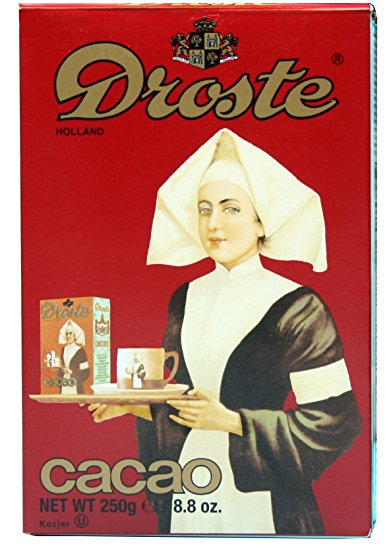
\includegraphics[height=1in]{background/pix/droste.jpg}
  \end{center}


  由于这款产品的关系，让一幅图片包含其自身的做法，有时也被称为
  德罗斯特效应。\index{Droste effect}
  % Can't get url to break: See also \protect\url{https://www.smithsonianmag.com/science-nature/fresh-off-the-3d-printer-henry-segermans-mathematical-sculptures-2894574/?no-ist}\index{self-reference}

  除了说谎者悖论，还有许多其他悖论。
  其中之一是 Quine（蒯因）悖论，\index{Quine's paradox}
  即一个断言自身为假的句子。


\begin{center}
    “当置于自身的引文之前时会产生假话” \\
    \quad 当置于自身的引文之前时会产生假话。
  \end{center}


  如果这个句子是假的，那么它所说的将是真话。
  如果这个句子是真的，那么它所说的就会成立，从而它就不是真的。

探讨这些及许多其他话题的一本精彩的大众读物是 \autocite{Hofstadter}。}。
换句话说，$\TM_m$ 的名字就是它的行为。

既然我们能够有效地从索引~$m$ 得到这台机器的源码，那么在某种意义上，这台机器是“知道”自己的源码的。
一个\citetext{\definend{蒯因（quine）}}{%
  以哲学家 Willard Van Orman Quine（威拉德·范·奥曼·蒯因）命名。}
是一个能输出自身源码的程序。
接下来，我们将逐步剖析构造一个蒯因的具体细节。\footnote{%
  最简单的这种程序会从磁盘上找到自己的源文件并把它打印出来。
  那是在作弊。}\index{quine program}\index{self reproducing program}
我们将使用 C 语言，因为它是低级语言，所以细节不会被隐藏。

我们可能会想，把源码本身作为一个字符串包含在源码中。
下面是一次这样的尝试，\footnote{%
  反斜杠-\protect\codeinline{n} 表示换行符。}
我们可以称之为 \codeinline{try0.c}。
但这太天真了。
那个字符串本身又得包含另一个字符串，如此等等。
就像小人理论一样，这会导致无穷倒退。
相反，我们需要一个程序，能以某种方式包含用于计算其自身一部分的指令。
\begin{lstlisting}
main() {
  printf("main(){\n ... }");
}
\end{lstlisting}

一种更巧妙的方法利用了我们对不动点定理的讨论，因为它在使用代码之前先提及代码。
这就是 \codeinline{try1.c}。\footnote{%
  \protect\codeinline{char *e="..."} 这个结构定义了一个字符串。
  在 C 语言的 \protect\codeinline{printf(...)} 命令中，第一个参数是一个字符串。
  在该字符串中，双引号会展开为单引号，
  \protect\codeinline{\%c} 会从随后的参数中取一个字符进行替换，
  而 \protect\codeinline{\%s} 会取一个字符串进行替换。}
\begin{lstlisting}
char *e="main(){printf(e);}"
main(){printf(e);};
\end{lstlisting}
以下是它的输出。
\begin{lstlisting}
main(){printf(e);};
\end{lstlisting}

将这一方法进一步升级，就得到了 \codeinline{try2.c}。
\begin{lstlisting}
char *e="main(){printf("char*e="");printf(e); printf("";\n");printf(e);"
main(){printf("char *e="");printf(e); printf("";\n");printf(e);}
\end{lstlisting}
这已经很接近了。
通过对一些换行符和引号进行转义\footnote{%
  数字 $10$ 是换行符的 ASCII 编码，34 是双引号的 ASCII 编码。}，
我们得到了这个能正常工作的程序 \codeinline{try3.c}。
\begin{lstlisting}
char *e="char*e="%c %s %c; %c main() {printf(e,34,e,34,10,10);}%c";
main(){printf(e,34,e,34,10,10);}
\end{lstlisting}

% A quine is a fixed point of an execution environment,
% when the execution environment is viewed as a function.
% Quines are possible in any complete model of
% computation; the exercises ask for them in a few languages.

% \subsection*{Know thyself}
% A program that prints itself can seem to be a parlor trick.
% But
% \citetext{for routines to have access to their code}{%
%   \definend{Introspection} is the ability to inspect code in the system,
%   such as to inspect the type of objects.
%   \definend{Reflection} is the ability to make modifications at runtime.}
% is useful.
% For example, to write a method \codeinline{toString(obj)}, you probably
% want your method to ask \codeinline{obj} for its source.
% Another example, more nefarious,
% is a computer virus that transmits copies
% of its code to other machines.

% \citetext{We will show how a routine can know its source}{%
%   This is derived from the wonderful presentation
%   in \autocite{Sipser}.}.
% We will start with an alternate
% presentation of a machine that prints itself.

% First, two technical points.
% One is that given two programs we can combine them into one, so that
% we run the first and then run the second.
% (Similarly,
% we can combine  two Turing  machines by
% renumbering the states so they do not conflict
% and then changing the final states in the first machine
% to have the number of the start state in the second.)

% The other point is
% that we have fixed a numbering of Turing machines that is
% `acceptable', meaning that there is a computable function from indices
% to machines and another computable function back.
% Write $\mathcal{T}$ for the set of Turing machines and
% let the function $\map{\strng}{\mathcal{T}}{\kleenestar{\B}}$
% input a Turing machine and return
% a standard bitstring representation of that machine (i.e., its source),
% let $\map{\mach}{\N}{\mathcal{T}}$
% input an index~$e$ and return the machine~$\TM_e$,
% and let $\map{\idx}{\kleenestar{\B}}{\N}$
% input the string representation of~$\TM_e$
% and return the index of that machine,~$e$
% (if the input string doesn't represent a Turing machine
% then it doesn't matter what this function does).
% Do this in such a way
% that $\idx$ is the inverse of the function $\composed{\strng}{\mach}$.

% Consider the machines sketched below.
% The first computes the
% function $\operatorname{echo}(\sigma,y)=\sigma$.
% Let it have index~$e_0$ and apply the \smn~theorem to get the
% family of machines sketched in the middle,  $\TM_{s(e_0,\sigma)}$,
% each of which ignores its input and just prints~$\sigma$.
% \begin{equation*}
%   \vcenteredhbox{\includegraphics{\asydir flowcharts/flowcharts13.pdf}}
%   \qquad
%   \vcenteredhbox{\includegraphics{\asydir flowcharts/flowcharts14.pdf}}
%   \qquad
%   \vcenteredhbox{\includegraphics{\asydir flowcharts/flowcharts15.pdf}}
% \end{equation*}
% On the right,
% $s(e_0,\sigma)$ is the index of the middle machine so
% $\composed{\strng}{\mach}(s(e_0,\sigma))$ is the standard string representation
% of the middle machine for~$\sigma$.
% Thus, if~$\sigma$ is the standard representation of a Turing machine~$\TM$ then
% when the machine on the right is done, the tape will contain only the standard
% representation of the middle machine for~$\sigma$, the machine that ignores
% its input and prints out~$\sigma$.
% Call the machine on the right~$\TM[Q]$ and call the function that it computes
% $\map{q}{\kleenestar{\Sigma}}{\kleenestar{\Sigma}}$.

% The machine that prints itself is a combination of two machines,
% $\TM[A]$ and~$\TM[B]$.
% Here's~$\TM[B]$.
% \begin{center}
%   \vcenteredhbox{\includegraphics{\asydir flowcharts/flowcharts16.pdf}}
% \end{center}
% The other machine is $\TM[A]=\TM_{s(e_0,\strng(\TM[B]))}$,
% which ignores anything on the tape and prints out
% the string representation of~$\TM[B]$.

% The action of the combination on an empty tape is that
% first the $\TM[A]$ part prints out the standard string representation
% $\strng(\TM[B])$.
% Then $\TM[B]$ reads it in as~$\beta$, computes
% $\alpha=\strng(\TM[A])$, concatenates the two string
% representations $\alpha\concat\beta$, and prints it.
% This is the string representation of itself, of the combination of
% $\TM[A]$ with~$\TM[B]$.

% To get a machine that computes with its own source
% we will extend this approach.
% The idea is to start with a machine~$\TM[C]$ that takes two inputs,
% a string representation of a machine and a string, and then
% get the desired machine~$\TM[D]$ that uses its own representation.

% \begin{theorem}
% For any Turing machine $\TM[C]$ that computes a two-input function
% $\map{c}{\kleenestar{\Sigma}\times\kleenestar{\Sigma}}{\kleenestar{\Sigma}}$
% there is a machine~$\TM[D]$ that computes a one-input function
% $\map{d}{\kleenestar{\Sigma}}{\kleenestar{\Sigma}}$
% where $d(\omega)=c(\strng(\TM[D]),\omega)$.
% \end{theorem}

% The machine~$\TM[D]$ is the combination of three machines, $\TM[A]$, $\TM[B]$,
% and~$\TM[C]$.
% First, as shown on the left,
% modify $\TM[Q]$ to write its output after a string already
% on the tape, because we need to leave the input~$\omega$ on the tape.
% \begin{center}
%   \vcenteredhbox{\includegraphics{\asydir flowcharts/flowcharts19.pdf}}
%   \qquad
%   \vcenteredhbox{\includegraphics{\asydir flowcharts/flowcharts20.pdf}}
% \end{center}
% Second, modify~$\TM[A]$ to be
% $\TM_{s(e_0,\strng(\TM[B])\concat\strng(\TM[C]))}$,
% which ignores anything on the tape and prints out
% the string representation
% of the combination of machines $\TM[B]$ and~$\TM[C]$.

% Next,
% as shown on the right, modify~$\TM[B]$ to
% input two strings, $\omega$ and~$\tau$.
% Apply~$q$ to the second to compute $\TM[A]$'s
% standard representation~$\alpha$.
% Print out the concatenation of $\alpha$ and~$\tau$, then a blank,
% and then the input~$\omega$.
% That has the form of two inputs;~finish by running the machine~$\TM[C]$ on
% them.

% \subsection*{Quining}
\citetext{动词 ‘to quine’}{%
  由 D~Hofstadter 发明。\index{Hofstadter, D}
  它可以追溯到哲学家 W~Quine 提出的陈述：
  \textit{“当置于自身引文之前时产生假话”当置于自身引文之前时产生假话}
  这句话具有悖论性质：如果它为真，则断言自身为假；如果为假，则必然为真。
  而且，它在没有直接自指的情况下做到了这一点。}
意思是：先写下一个句子片段，然后再写一遍，但这次要给它加上引号。
例如，从 `say` 我们得到 “say ‘say’.”。
另一个例子是 “quine ‘quine’.”。
这是自复制程序的语言学类比，其中第二个词扮演了传统程序/数据分离中数据的角色，
% http://www.madore.org/~david/computers/quine.html
这个角色与 \protect\codeinline{try3.c} 的第一行字符串所扮演的角色相同。
  %  ="char*e="%c %s %c; %c main() {printf(e,34,e,34,10,10);}%c";}
在“制造这台机器，然后执行这台机器”中，“制造”一词扮演的也是这个角色。

\citetext{我们可以用代码来表达这一点}{%
  本小节这一部分的内容源自
  \autocite{boro}\Dash
  “Boro”这个名字也来源于此\Dash 以及 \autocite{Avigad}。}。
首先考虑“引用”。
为了执行某个操作，我们通常定义一个函数，然后像 \codeinline{(f 1 2)} 这样调用它。
因此，如果我们想生成一个包含三个字符串的列表，那么下面的代码
\begin{lstlisting}
> (Boro is reading)
\end{lstlisting}
会产生错误：\codeinline{Boro:}\codeinline{undefined}。
我们必须告诉 Racket 不要对这些内容求值，在这个例子中，就是不要按通常方式对列表求值（将第一个条目当作函数，然后将其应用于其他条目的求值结果）。
\begin{lstlisting}
> (quote (Boro is reading))
'(Boro is reading)
\end{lstlisting}
有一个方便的单字符快捷方式。
\begin{lstlisting}
> '(Boro is reading)
'(Boro is reading)
\end{lstlisting}
我们可以把它做成一个函数。
\lstinputlisting[firstline=12,lastline=13]{scheme/background/quine-boro.rkt}
\begin{lstlisting}
> (P 'reading)
'(Boro is reading)
\end{lstlisting}
使用它就能得到\definend{对角化}例程。\index{diagonalization!routine}
\lstinputlisting[firstline=15,lastline=16]{scheme/background/quine-boro.rkt}
\begin{lstlisting}
> (Diag P 'reading)
'(Boro is '(Boro is reading))
\end{lstlisting}
这里是一个蒯因。
\lstinputlisting[firstline=24,lastline=25]{scheme/background/quine-boro.rkt}
\begin{lstlisting}
> (Quine-1 'reading)
'(reading 'reading)
> (Quine-1 'Quine-1)
'(Quine-1 'Quine-1)
\end{lstlisting}
% For a version that does not depend on the definitions use this.
% \begin{lstlisting}
% > ((lambda (x) (list x (list 'quote x)))
%  '(lambda (x) (list x (list 'quote x))))
% '((lambda (x) (list x (list 'quote x))) '(lambda (x) (list x (list 'quote x))))
% \end{lstlisting}
% The \codeinline{(lambda (x) ...)} construct is how Racket
% defines a function of one input without giving it a name
% (the term `lambda' comes from Church's Lambda Calculus).

\margingraphic{0.18\textwidth}{background/pix/thompson.jpg}{%
  \label{fig:thompson}\href{https://en.wikipedia.org/wiki/Ken_Thompson}{Ken Thompson（肯·汤普森） b~1943}}\index{Thompson, K!picture} % http://images.computerhistory.org/fellows/1997_ken_thompson.jpg
\subsection*{对信任的反思}\index{Reflections on Trusting Trust@\textit{Reflections on Trusting Trust}}
K~Thompson 是 UNIX 操作系统的两位主要创造者之一。
他职业生涯的大部分时间都在贝尔实验室工作，并且是 C 语言开发的核心人物。
他是正则表达式使用的先驱，并草拟了 Unicode 的 UTF-8 编码的定义。
近年来，他也是谷歌 Go 语言的创建者之一。

他曾获得计算机科学最高荣誉——图灵奖。
他在获奖演讲的开头是这样说的。

\begin{quotation}
上大学那会儿，还没有电子游戏，我们常常靠出编程题来互相消遣。
其中最受欢迎的题目之一，就是编写最短的自复制程序。
既然这是一项脱离现实的练习，
通常的工具就是 FORTRAN。
事实上，选择 FORTRAN 作为语言的理由，
和三人两足赛跑流行的理由是一样的。
\ldots{}\sentencespace
\end{quotation}

\vspace{-1.65ex} % picked by eye


\begin{quotation} % adding the extra quotation env makes K Thompson's outdent better
更精确地说，这个问题要求你编写一段源程序，
当其被编译并执行后，将产生一份与其源代码完全相同的副本作为输出。
% If you have never done this, I urge you to try it on your own.
% The discovery of how to do it is a revelation that far surpasses any
% benefit obtained by being told how to do it.
% The part about ``shortest'' was just an incentive to demonstrate skill
% and determine a winner.
\end{quotation}

这篇著名的文章构造了一个蒯因，
并展示了此类代码的存在如何构成一种极其微妙且几乎无法检测的安全威胁。
Thompson 的整个演讲 \autocite{Thompson} 流传很广；每个人都应该读一读。

% ...........................................
% \begin{exercises}
% \begin{exercise}
% Produce a Racket quine.
% \begin{credit}
%   \url{https://research.swtch.com/zip}
%   and
%   \href{http://cs.brown.edu/courses/gs019/asgn/hw3.sol.pdf}{Kevin Matulef}
% \end{credit}
% \begin{answer}
% % Here is a classic.
% % \begin{lstlisting}
% % ((lambda (x) `(,x ',x))
% % '(lambda (x) `(,x ',x)))
% % \end{lstlisting}
% %
% % This is due to Kevin Matulef.  % http://cs.brown.edu/courses/gs019/asgn/hw3.sol.pdf
% \lstinputlisting[firstline=3]{scheme/background/quine.rkt}
% \end{answer}
% \end{exercise}

% \begin{exercise}
% Produce a Python quine.
% \begin{credit}
%   \url{http://en.wikipedia.org/wiki/Quine_%28computing%29}
% \end{credit}
% \begin{answer}
% The python3 code
% \begin{lstlisting}
% # quine.py
% s = r"print('s = r\"' + s + '\"' + '\nexec(s)')"
% exec(s)
% \end{lstlisting}
% gives this command line output.
% \begin{lstlisting}
% $ python3 quine.py
% s = r"print('s = r\"' + s + '\"' + '\nexec(s)')"
% exec(s)
% \end{lstlisting} %$
% \end{answer}
% \end{exercise}

% % \begin{exercise}  %  p 75
% % \begin{credit}
% %   J~Avigad Computability and Incompleteness Lecture notes, % p 75
% %   \url{https://www.andrew.cmu.edu/user/avigad/Teaching/candi_notes.pdf}
% % \end{credit}
% % Consider a Scheme function \codeinline{diag} that is given a
% % string~$\sigma$ and returns a string with each instance of \str{x} in
% % $\sigma$ replaced with a quoted version of $\sigma$.
% % Thus \codeinline{diag("hello x world")} returns
% % \str{hello 'hello x world' world}.
% % Show that \codeinline{print(diag('print(diag(x))'))} is a quine.
% % \begin{answer}
% % \begin{lstlisting}
% % (define (diag s)
% %       (regexp-replace #rx"x" s s))
% % \end{lstlisting}
% % \end{answer}
% % \end{exercise}

% % \begin{exercise}
% % Write a program that defines a function
% % $f$ taking a string as input, and produces its output by applying
% % $f$ to its source code. For example, if $f$
% % reverses the given string, then the program should outputs its source code
% % backwards.
% % \end{exercise}

% % \begin{exercise}
% % Write a two-level polyglot quine, a program in one language
% % that outputs a program in a second language, which outputs the original program.
% % \end{exercise}
% \end{exercises}
\index{self reproduction|)}

% =======================================================
% \extra{Computer viruses}

% =======================================================
% \extra{A Universal Turing machine}

% =======================================================
\extra{忙海狸}\index{Busy Beaver|(}
% % \urldef{\radourl}{\url{https://math.osu.edu/about-us/history/tibor-rad%C3%B3}}
% \margingraphic{0.18\textwidth}{background/pix/rado1.png}{\label{fig:rado}\href{https://en.wikipedia.org/wiki/Tibor_Rad\%C3\%B3}{Tibor Rad\'o 1895--1965}}\index{Rado, T@Rad\'o, T!picture} % https://math.osu.edu/about-us/history/tibor-rad%C3%B3
对于任意~$n\in\N$，状态数不超过 $n$~的 Turing 机构成的集合是有限的。
因此，该集合中在空白纸带上会停机的 Turing 机 $\TM_e$ 只有有限多台。
我们可以思考，通过理解这些小型机器的行为，
我们能否获得关于计算（尤其是 Turing 机）的一般性洞见——例如，大多数 $n$ 状态 Turing 机会停机，还是只有少数会停机？

定义函数
$\map{\definend{\BB}}{\N}{\N}$ % \index{BB@$\BB$ (Busy Beaver) function}
给出最小步数，使得所有状态数为~$n$ 且在空白纸带上最终会停机的机器，到该步数时均已停机。
同时令
$\map{\definend{\Sigma}}{\N}{\N}$ % \index{Sigma@$\Sigma$ function}
为 $n$ 状态 Turing 机（从空白纸带启动）停机后留在纸带上的 \str{1} 数量的最大值。

\begin{theorem}[Rad\'o, 1962]
函数 $\BB$ 和 $\Sigma$ 是不可计算的。
\end{theorem}

\begin{proof}
如果~$\BB$ 是可计算函数，那么要判断某台 $\TM_e$ 在输入~$e$ 上是否停机，
我们只需让它运行 $\BB(n)$ 步。
如果 $\TM_{e}(e)$ 届时仍未停机，它就永远不会停机。
因此，$\BB$ 的可计算性将与停机问题（\HP）的不可解性相矛盾。
函数 $\Sigma$ 的情况类似，其证明留作练习 \zcref{exer:SigmaNotComputable}。
\end{proof}

这个 $\BB$ 看起来可能只是众多不可计算函数中的又一个而已。
然而，它有一个有趣的性质：任何增长速度比它快的函数 $f$——
即对所有足够大的~$n$ 满足 $f(n)\geq \BB(n)$——
同样也是不可计算的，其论证方法与前面证明中的相同。
于是，我们对什么使得一个函数不可计算获得了一种洞见：一种方式是增长得比任何可计算函数都快。\footnote{%
  注意这与 Ackermann 函数的联系，我们曾指出 Ackermann 函数不是原始递归的，
  因为它增长得比任何原始递归函数都快。}

% \margingraphic{0.25\textwidth}{background/pix/beaver.jpg}{\label{fig:beaver}\href{http://commons.wikimedia.org/wiki/File:Beaver_\%28PSF\%29.jpg}{Rare moment of rest}}
% \urldef{\radourl}{\url{https://math.osu.edu/about-us/history/tibor-rad%C3%B3}}
\margingraphic{0.18\textwidth}{background/pix/rado1.png}{\label{fig:rado}\href{https://en.wikipedia.org/wiki/Tibor_Rad\%C3\%B3}{Tibor Rad\'o 1895--1965}}\index{Rado, T@Rad\'o, T!picture} % https://math.osu.edu/about-us/history/tibor-rad%C3%B3
\definend{忙海狸问题}\index{Busy Beaver problem@\probname{Busy Beaver} problem}
是：\citetext{哪台 $n$ 状态 Turing 机在停机前能做最多的计算工作}{%
  R~H Bruck 曾写道 \autocite{Bruck}：
  “我可以把高速计算机比作一支巨大而笨拙的铅笔，
  它需要很长时间才能削好，也无法用通常的方式用手指握持，
  给人以能响应我心意的错觉；
  但它却配备了一台相当精密的引擎，
  只要我愿意让它在很大程度上支配书写的主题，
  它就会像疯了一样疯狂书写。”
  忙海狸机就是该规模下最疯狂的书写者。
}？

\citetext{可以把这看作一场竞赛}{%
  关于这个主题有两个非常精彩的视频：
  YouTube 频道 Mutual Information 的
  \href{https://www.youtube.com/watch?v=kmAc1nDizu0}{\textit{计算的边界}}
  和
  \href{https://www.youtube.com/watch?v=jlh21U2texo}{\textit{在计算的边界会发生什么？}}。}
看谁能构造出达到极限值~$\BB(n)$ 或~$\Sigma(n)$ 的机器。\footnote{%
  在这个问题由 T~Rad\'o 首次提出后的许多年里，
  竞赛主要围绕 $\Sigma$ 展开。
  不过，最近大家更常讨论 $\BB$。
  无论如何，这两者关系非常密切。}
计算需要规则，此处的传统是固定一种 Turing 机的定义：它具有一端无限延伸的纸带，
使用两个纸带符号 \str{1} 和~\str{B}，
有一个不计入机器状态总数的独立停机状态，
机器从空白纸带开始运行，
且转移的形式为
$\Delta(\text{state}, \text{tape symbol})
  =\sequence{\text{state}, \text{tape symbol}, \text{head shift}}$。

\subsection*{已知结果}
\citetext{在 1962 年的论文中，Rad\'o}{%
  这篇论文 \autocite{Rado} 异常清晰且有趣。}
解决了 $n=0$、$n=1$ 和 $n=2$ 的情况
（$n=0$ 是平凡的，因为此时机器仅由停机状态组成）。
1964 年，Rad\'o 和 Lin 证明了 $\Sigma(3)=6$。


\begin{example}
这是三状态的忙海狸机器，停机状态是~$q_3$。
\begin{center}  \small
\begin{transitionfunction}
        &\str{B}  &\str{1}  \\ \cline{2-3}
  $q_0$ &$q_1,\str{1},R$  &$q_3,\str{1},R$        \\
  $q_1$ &$q_2,\str{B},R$  &$q_1,\str{1},R$        \\
  $q_2$ &$q_2,\str{1},L$  &$q_0,\str{1},L$
\end{transitionfunction}
\end{center}
\end{example}


1983 年，A~Brady 证明了 $\Sigma(4)=13$ 和 $\BB(4)=107$。

\citetext{2024 年，一组研究人员}{%
  参见 \autocite{Brubaker}} 通过互联网协作，并使用 Coq 证明验证系统，证明了
$\Sigma(5)=4\,098$ 以及 $\BB(5)=47\,176\,870$。
他们的机器计算 $g(0)$, $g(g(0))$, \ldots{} 直到停机，其中
$g$ 是这个函数。
\begin{equation*}
  g(n)=
  \begin{cases}
    (5n+18)/3  &\case{if $n$ leaves a remainder of $0$ on division by $3$}  \\
    (5n+22)/3  &\case{if $n$ leaves a remainder of $1$}  \\
    \text{停机}&\case{otherwise}
 \end{cases}
\end{equation*}

下表总结了
\citetext{当前记录}{%
  最新的是 BB(6) 的结果，由 BBchallenge 团队成员 mxdys 于 2025 年 6 月得出。}。

\begin{center}\small
  \begin{tabular}{r|cccccc}
    $n$         &$1$  &$2$  &$3$  &$4$   &$5$           &$6$ \\ \cline{2-7}
    \begin{tabular}[t]{@{}r@{}}
      $\BB(n)$  \\
      $\Sigma(n)$
    \end{tabular}
    &\begin{tabular}[t]{@{}r@{}}
      $1$ \\
      $1$
    \end{tabular}
    &\begin{tabular}[t]{@{}r@{}}
      $6$ \\
      $4$
    \end{tabular}
    &\begin{tabular}[t]{@{}r@{}}
      $21$ \\
      $6$
    \end{tabular}
    &\begin{tabular}[t]{@{}r@{}}
      $107$ \\
      $13$
    \end{tabular}
    &\begin{tabular}[t]{@{}r@{}}
      $47\,176\,870$  \\
      $4\,098$
    \end{tabular}
    &\rule{0em}{2.25ex}\begin{tabular}[t]{@{}l@{}}
      $\geq \prescript{9}{}{\prescript{2}{}{\prescript{2}{}{2}}}$
      \rule{0pt}{13pt}
      \\
      $\geq \prescript{15}{}{10}$ %\uparrow\uparrow 15
    \end{tabular}
  \end{tabular}
\end{center}

左上标记法表示四级超运算，即迭代幂运算。
因此，$\prescript{9}{}{2}$ 表示 $2$ 的 $2$ 次幂的 $2$ 次幂 \ldots{}，共迭代九次。

\subsection*{如何寻找这些值}
在 $n=2$ 之后，解决这个问题的显然方法是使用广度优先搜索：$n$~状态的机器只有有限多台，因此
让它们全部在空白纸带上运行，进行交错并行，
然后静观其变。
这能快速判定大量机器的情况。
当然，其中一些机器不会停机，或者运行时间超出我们的耐心。
对于其中部分机器，从其源代码很容易判断其行为，我们有望将范围快速缩小到相对较少的机器进行深入研究，
从而通过穷举法找到该~$n$ 的答案。\footnote{%
  \protect\citetext{Brady}{参见 \protect\autocite{Brady}} 报告称，对于 $n=4$，
  这样的机器有 $5\,280$ 台。}

但是，如果对于某个~$n$，我们找到一台计算着某些我们未知之物的机器呢？
例如，如果 $n$ 足够大，以至于能容许一台机器当且仅当找到
\citetext{奇完全数}{%
  如果一个数等于其所有真因子之和，则称为完全数。
  例如，$6=1+2+3$。
  偶完全数是存在的，但我们不知道奇完全数是否存在。}
时才停机呢？
$n=6$ 的情况似乎就存在一台类似的机器。

如需了解更多信息，有许多网站涵盖了这一主题，包括最新的结果。
除了维基百科页面外，最经典的网站是 \href{https://bbchallenge.org}{\texttt{bbchallenge.org}}。
有些网站讨论了机器标准的变体，例如考虑
\citetext{具有三个或更多符号的机器}{%
  具有三个状态和三个符号的机器的情况仍然未知。
  求解它需要解决一个类似 Collatz 的问题，目前无人能做到。
  参见
  \url{https://www.sligocki.com/2023/10/16/bb-3-3-is-hard.html}。}。

忙海狸数不仅极难寻找，而且在某一点之后会变得根本无法求解。
2016 年，A~Yedida 和 S~Aaronson 得到了一个 $n$，使得
\citetext{$\BB(n)$ 不可知}{%
  参见 \autocite{Aaronson16} 以及优秀的综述 \autocite{Aaronson20}
  和 \autocite{Aaronson25}。
  另见 \url{https://www.quantamagazine.org/the-busy-beaver-game-illuminates-the-fundamental-limits-of-math-20201210/}。}。
为此，他们创建了一种编程语言，其程序可编译成 Turing 机。
利用该语言，他们构造了一台
\citetext{7918 状态的 Turing 机}{%
  所需的状态数此后已被减少。
  截至本书写作时，它已降至 $748$ 个状态。
  参见 J~Riebel 优秀的学士学位论文：
  \url{https://www.ingo-blechschmidt.eu/assets/bachelor-thesis-undecidability-bb748.pdf}。}，
如果\citetext{数学的标准公理}{%
  这是 ZFC，即带有选择公理的 Zermelo–Fraenkel 公理。
  （此外，他们还假定了静止 Ramsey 性质假设。）}中存在矛盾，则该机停机；
如果这些公理是一致的，则永不停机。
我们相信这些公理是一致的，因此我们相信这台机器不会停机。
然而，Gödel 第二不完备定理表明，无法用公理本身来证明这些公理是一致的。
因此，在这种情况下，\probname{Busy Beaver} 问题的解是不可知的，因为即使我们得到了数 $\BB(n)$，也无法用我们的公理证明它是正确的，即证明这台机器会停机。
% (They also produced an explicit
% Turing machine that halts if and only if there is a counterexample to Goldbach’s
% conjecture, and one that halts if and only if the Riemann hypothesis
% is false.)

总而言之，函数不可计算的一种方式是其增长速度快于任何可计算函数。
但要注意，这并不是唯一的方式。
存在一些函数，它们的增长速度慢于某些可计算函数，却仍然是不可计算的。

\begin{exercises}
% \recommended
% \begin{exercise}
% Give the computation history, the sequence of configurations, that come from
% running the three-state Busy Beaver machine.
% \hint~you can run it on the Turing machine simulator.
% \end{exercise}


\begin{exercise}
讨论中用到的这种风格的 Turing 机共有多少台？
\begin{answer}\verified
函数 $\Delta$ 有 $n\cdot 2$ 个输入和 $(n+1)\cdot  2\cdot 2$ 个输出。
因此共有 $(2n)^{4(n+1)}$ 台机器。
\end{answer}
\end{exercise}

\recommended


\begin{exercise}
编写并运行一个例程来计算 $g(0)$、$g(g(0))$，……。
\begin{answer}\verified
\figureref{fig:RacketBB5} 中的 Racket 代码可以计算它。
\begin{figure}
  \centering
  \lstinputlisting[firstline=3]{background/scheme/BB5.rkt}
  \caption{产生计算 $\BB (5)$ 过程中所发现值的 Racket 代码。}
  \label{fig:RacketBB5}
\end{figure}
值依次为 $6$、
$16$、
$34$、
$64$、
$114$、
$196$、
$334$、
$564$、
$946$、
$1584$、
$2646$、
$4416$，
$7366$、
以及 $12284$。
\end{answer}
\end{exercise}

% \recommended
% \begin{exercise}
% \begin{exparts*}
% \item
% How many Turing machines with tape alphabet $\set{\str{B},\str{1}}$
% are there having one state?
% \item
% Two?
% \item
% How many with $n$~states?
% \end{exparts*}
% \end{exercise}

% \begin{exercise}
% How many Turing machines are there, with a tape alphabet
% $\Sigma$ of $n$ characters and having $n$~states?
% \begin{answer}
% $\bigl( 2(c+1)(n+2) \bigr)^{(c+1)n}$
% \end{answer}
% \end{exercise}

% \begin{exercise}
% Give $\TM[M]_1$ and $\TM[M]_2$, the Turing machines
% having $1$ and~$2$ states that write $1$ and $2$-many \str{1}'s to a blank tape.
% \end{exercise}

\recommended


\begin{exercise}
给出一个最终将超过任何可计算函数的函数的对角化构造。
\begin{answer}\verified
本题并未要求我们构造一个可计算函数；事实上，这样的可计算函数根本不存在。

如果 $\TMfcn_0(0)$ 收敛，则定义 $f(0)$ 为 $1+\TMfcn_0(0)$；否则定义 $f(0)=1$。
（注意 $f$ 不是可计算函数。）
类似地，定义 $f(1)$ 为 $1+f(0)$、$1+\TMfcn_0(1)$ 与 $1+\TMfcn_1(1)$ 三者的最大值，
若后两项中任意一项发散，则不将其计入最大值中。
对所有 $n$ 同理定义。

更形式化地，若 $\TMfcn_e(x)$ 收敛，则定义 $F(e,x)$ 为 $\TMfcn_e(x)$，否则为 $0$。
那么 $f(i)$ 就是 $\set{F(0,i),\ldots F(i,i)}$ 的最大值再加 $1$。
\end{answer}
\end{exercise}

\recommended

\begin{exercise}
证明存在不可计算函数，其增长速度不快于可计算函数 $f(x)=1$。
\hint~用可数性论证。
\begin{answer}
根据提示，注意到输出在集合 $\set{0,1}$ 中的函数有不可数多个，
即每个输出都小于或等于 $1$。
Turing 机只有可数多个，所以可计算函数只有可数多个，
因此输出以 $1$ 为界的可计算函数也只有可数多个。
故存在输出以 $1$ 为界的不可计算函数。
\end{answer}
\end{exercise}

\begin{exercise} \label{exer:SigmaNotComputable}
这是关于 $\Sigma$ 不可计算的证明。
设 $\map{f}{\N}{\N}$ 是任意全可计算函数。
我们将证明对无穷多个 $n$ 有 $\Sigma(n)>f(n)$，因此 $\Sigma\neq f$。
\begin{exparts}
\item
证明存在一台具有 $j$ 个状态的 Turing 机 $\TM[M]_j$，
它能在空白纸带上写下 $j$ 个 \str{1}。
\item
令 $\map{F}{\N}{\N}$ 为这个函数。
\begin{equation*}
  F(m) % = \sum_{0\leq i< m+1} f(i)+i^2  % using \Sigma so omit summation
       = (f(0)+0^2)+(f(1)+1^2)+(f(2)+2^2)+\cdots+(f(m)+m^2)
\end{equation*}
论证它具有以下三个性质：若 $0<m$，则 $f(m)<F(m)$，
且 $m^2\leq F(m)$，
以及 $F(m)<F(m+1)$。
\item
下面的插图展示了两台 Turing 机的组合。
在右侧，我们将左侧第一台机器的接受状态与第二台机器的初始状态合并。
\begin{center}
  \vcenteredhbox{\includegraphics{\asydir busybeaver/busybeaver01.pdf}}
  \hspace{2.5em}
  \vcenteredhbox{\includegraphics{\asydir busybeaver/busybeaver02.pdf}}
\end{center}
考虑 Turing 机 $\TM$，它先执行 $\TM[M]_j$，
然后执行 $\TM[M]_F$，接着再执行一次 $\TM[M]_F$。
证明它的生产力为 $F(F(j))$，且具有 $j+2n_F$ 个状态。

\item
最后，与具有 $j+2n_F$ 个状态的忙海狸机比较。
根据定义，
$F(F(j))\leq \Sigma(j+2n_F)$。
因为 $n_F$ 是机器 $\TM[M]_F$ 的状态数，为常数，所以关系 $j+2n_F\leq j^2< F(j)$
对足够大的 $j$ 成立。
请论证
$f(j+2n_F) \leq \Sigma(j+2n_F)$。
\end{exparts}
\begin{answer}\verified
\begin{exparts}
\item
最好用一个例子来回答：这里是 $\TM[M]_4$。
\begin{center}
  \includegraphics{\asydir busybeaver/busybeaver00.pdf}
\end{center}
\item
第一个性质成立是因为 $f(m)$ 是 $F(m)$ 表达式中的一个求和项；
类似地，第二个性质成立是因为 $m^2$ 也是一个求和项。
第三个性质成立是因为当 $m>0$ 时所有求和项均为正数。

\item
如果从空白纸带开始，这台机器首先产生 $j$ 个 \str{1}，
然后产生 $F(j)$ 个 \str{1}，最终在纸带上留下 $F(F(j))$ 个 \str{1}。
因此其生产力为 $F(F(j))$。

\item
由于 $F$ 严格递增，$F(j+2n_F)<F(F(j))$。
结合得到
$
   f(j+2n_F) <
   F(j+2n_F) <
   F(F(j))
   \leq \Sigma(j+2n_F)$，
如所需。
\end{exparts}
\end{answer}
\end{exercise}

% Copy this back to the proof?
% For $\Sigma$,
% let $\map{f}{\N}{\N}$ be any total computable function.
% We will show that
% $\Sigma(n)>f(n)$ for infinitely many~$n$,
% and so $\Sigma\neq f$.
%
% First note that there is a Turing Machine $\TM[M]_j$
% having $j$~many states that writes $j$-many \str{1}'s to a blank tape.
% For instance, here is $\TM[M]_4$.
% \begin{center}
%   \includegraphics{\asydir busybeaver/busybeaver00.pdf}
% \end{center}
% Also note that we can compose two Turing machines.
% The illustration below shows two machines on the left.
% On the right, we have combined the final states
% of the first machine with the start state of the second.
% \begin{center}
%   \vcenteredhbox{\includegraphics{\asydir busybeaver/busybeaver01.pdf}}
%   \hspace{2.5em}
%   \vcenteredhbox{\includegraphics{\asydir busybeaver/busybeaver02.pdf}}
% \end{center}
%
% Let $\map{F}{\N}{\N}$ be this function.
% \begin{equation*}
%   F(m) % = \sum_{0\leq i< m+1} f(i)+i^2  % using \Sigma so omit summation
%        = (f(0)+0^2)+(f(1)+1^2)+(f(2)+2^2)+\cdots+(f(m)+m^2)
% \end{equation*}
% It has the properties:~if $0<m$ then $f(m)<F(m)$,
% and $m^2\leq F(m)$,
% and $F(m)<F(m+1)$.
% It is intuitively computable so Church's Thesis says there is a
% Turing machine $\TM[M]_F$ that computes it.
% Let that machine have $n_F$~many states.
%
% Now consider the Turing machine $\TM$
% that performs $\TM[M]_j$ and follows that with the machine
% $\TM[M]_F$, and then follows that with another copy of the machine
% $\TM[M]_F$.
% If started on a blank tape this machine will first produce $j$-many \str{1}'s,
% then produce $F(j)$-many \str{1}'s, and finally will leave the tape with
% $F(F(j))$-many \str{1}'s.
% Thus its productivity is
% $F(F(j))$.
% It has $j+2n_F$ many states.

% Compare that with the $j+2n_F$-state Busy Beaver machine.
% By definition
% $F(F(j))\leq \Sigma(j+2n_F)$.
% Because $n_F$ is constant (it is the number of states in
% the machine $\TM[M]_F$), the relation $j+2n_F\leq j^2< F(j)$
% holds for sufficiently large~$j$.
% Since $F$ is strictly increasing, $F(j+2n_F)<F(F(j))$.
% Combining gives
% $
%    f(j+2n_F) <
%    F(j+2n_F) <
%    F(F(j))
%    \leq \Sigma(j+2n_F)$,
% as required.

\end{exercises}
\index{Busy Beaver|)}

% =============================
% For defn of \cantorfile see src/directory.tex
\extra{用代码实现 Cantor 对应}  \label{sec:CantorInCode}
在本节中，我们以最直接的方式证明 $\N$ 和 $\N\times\N$ 之间的 Cantor 对应是能行的：我们给出代码。

回顾在下表中
\begin{equation*}
  \begin{array}{r|cccccc@{\hspace{6pt}}c}
    \tabulartext{$n\in\N$}
      &0 &1 &2 &3 &4 &5 &\ldots
      \\ \cline{2-8}
    \tabulartext{$\sequence{i,j}\in\N\times\N$}
      &\sequence{0,0} \rule{0em}{2ex} % make room above angle brackets
      &\sequence{0,1}
      &\sequence{1,0}
      &\sequence{0,2}
      &\sequence{1,1}
      &\sequence{2,0}
      &\ldots
  \end{array}
\end{equation*}
%</table:CrossProductCorrespondence>
%<*def:PairingFcn>
从顶行到底行的映射是 Cantor
配对函数\index{pairing function}\index{function!pairing}，
因为它输出数对；而从底行到顶行的逆映射是
解配对函数\index{unpairing function}\index{function!unpairing}。

首先是解配对。
给定 $\sequence{x,y}$，我们用 $1+2+\cdots n=n(n+1)/2$ 确定它所在的对角线，
\lstinputlisting[firstline=17,lastline=22]{\cantorfile}
然后利用它来找到值 $(1+2+\cdots x)+y$。
\lstinputlisting[firstline=33,lastline=38]{\cantorfile}

使用这个函数很容易。
\begin{lstlisting}
$ racket
Welcome to Racket v8.3 [cs].
> (require "counting.rkt")
> (cantor-unpairing 1 1)
4
> (cantor-unpairing 34 10)
1024
>
\end{lstlisting} % $

我们可能会想，\codeinline{cantor-unpairing} 的参数
应该是如上所得的两个数 $x$ 和 $y$，
还是数对 $\sequence{x,y}$。
但这并不太重要，因为如果我们需要这个数对，
可以改用 \codeinline{apply} 操作符。
\begin{lstlisting}
> (cantor-unpairing 10 12)
263
> (apply cantor-unpairing '(10 12))
263
\end{lstlisting} % $

接下来，介绍配对函数。
给定一个自然数 $c$，为了找到对应的数对 $\sequence{x,y}$，我们首先要找到它落在哪条对角线上。
对角线为 $d(x,y)=x+y$，设对应的三角数为$t(x,y)=d(d+1)/2=(d^2+d)/2$。
于是有 $0=d^2+d-2t$。
应用熟悉的公式$(-b\pm\sqrt{b^2-4ac})/(2a)$可得：
\begin{equation*}
  d=\frac{-1+\sqrt{1-4\cdot 1\cdot (-2t)}}{2\cdot 1}
   =\frac{-1+\sqrt{1+8t}}{2}
\end{equation*}
（我们只保留了 $\pm$ 中的 $+$ 号，因为另一个根是负数。）
给定配对函数的输入~$c$，为了找到包含满足 $\pair(x,y)=c$ 的数对 $\sequence{x,y}$ 的那条对角线的编号，
\citetext{使用取底函数}{%
  设第 $n$ 个三角数为
  $t(n)=0+1+\cdots+n=n(n+1)/2$。
  函数~$t$ 是单调递增的，并且存在无穷多个三角数。
  因此，对于每个自然数~$c$，都存在唯一的最大三角数 $t(n)$，使得 $c=t(n)+k$ 对某个~$k\in\N$ 成立。
  因为$t(n+1)=t(n)+n+1$，我们看到 $k<n+1$，即 $k\leq n$。
  所以，要从数对的 Cantor 编号~$c$ 计算对角线编号~$d$，我们有$(1/2)d(d+1)\leq c< (1/2)(d+1)(d+2)$。
  应用二次求根公式的左右两部分，得到$(1/2)(-3+\sqrt{1+8c})<d\leq (1/2)(-1+\sqrt{1+8c})$。
  令$(1/2)(-1+\sqrt{1+8c})$为 $\alpha$，则有$c\in\rightclosed{\alpha-1}{\alpha}$，因此 $d=\floor{\alpha}$。
  \autocite{222835}}，
$d=\floor{(-1+\sqrt{1+8c})/2}$。
% \footnote{
%   The code for \codeinline{diag-num} has and implementation detail of interest.
%   The code leads to numbers large enough to
%   give floating point overflows.
%   For instance, \protect\codeinline{(cantor-n 1 2 3 4 5 6 7)} returns
%   \protect\codeinline{1.05590697087673e+55}.
%   }

\lstinputlisting[firstline=58,lastline=63]{\cantorfile}
然后，通过查看~$c$ 沿这条对角线走了多远，我们就能得到 $\sequence{x,y}$。
\lstinputlisting[firstline=75,lastline=81]{\cantorfile}

\noindent 以自然的方式使用它。

\begin{lstlisting}
> (cantor-pairing 15)
'(0 5)
> (cantor-pairing (cantor-unpairing 10 12))
'(10 12)
\end{lstlisting}

有了这些，我们就可以重现本节开头的表格了。

\begin{lstlisting}
> (for ([i '(0 1 2 3 4 5)])
     (displayln (cantor-pairing i)))
(0 0)
(0 1)
(1 0)
(0 2)
(1 1)
(2 0)
\end{lstlisting}

扩展到三元组是直截了当的。
这些例程的命名或许不太恰当\Dash 它们可能更适合被命名为
\codeinline{cantor-tupling-3} 和 \codeinline{cantor-untupling-3}\Dash
但我们将沿用已有的名称。

\lstinputlisting[firstline=107,lastline=110]{\cantorfile}
\lstinputlisting[firstline=122,lastline=126]{\cantorfile}

\noindent
使用这些例程也很直接。

\begin{lstlisting}>
> (cantor-pairing-3 172)
'(1 2 3)
> (for ([i '(0 1 2 3 4 5 6 7 8 9)])
     (displayln (cantor-pairing-3 i)))
(0 0 0)
(0 0 1)
(1 0 0)
(0 1 0)
(1 0 1)
(2 0 0)
(0 0 2)
(1 1 0)
(2 0 1)
(3 0 0)
\end{lstlisting}

类似的例程也适用于四元组。

\lstinputlisting[firstline=147,lastline=150]{\cantorfile}
\lstinputlisting[firstline=162,lastline=167]{\cantorfile}

以下是前几个四元组。

\begin{lstlisting}
> (for ([i '(0 1 2 3 4 5 6)])
    (displayln (cantor-pairing-4 i)))
(0 0 0 0)
(0 0 0 1)
(1 0 0 0)
(0 1 0 0)
(1 0 0 1)
(2 0 0 0)
(0 0 1 0)
\end{lstlisting}

% From url.sty; need this because the url has a percent sign in it.
\urldef{\yagni}\url{https://en.wikipedia.org/wiki/You_aren%27t_gonna_need_it}
三元组和四元组的例程表明，存在一个通用的模式。
何妨一试，就当好玩，
\citetext{我们可以扩展到任意大小的元组}{%
  参见 \yagni。}。

对于函数$\map{\unpair}{\N^k}{\N}$（我们也称它为 $\cantor$），我们可以通过查看输入参数的个数来确定 $k$。
因此，\codeinline{cantor-unpairing-n} 通过接受任意长度的元组，推广了
\codeinline{cantor-unpairing}、\codeinline{cantor-unpairing-3} 等函数。

\lstinputlisting[firstline=195,lastline=203]{\cantorfile}

\begin{lstlisting}
> (cantor-unpairing-n 0 0 1 0)
6
> (cantor-unpairing-n 1 2 3 4)
159331
\end{lstlisting}

要推广到函数$\map{\pair}{\N}{\N^k}\!$，
棘手的地方在于，这个例程无法知道目标元数~$k$，我们必须单独指定它。

\lstinputlisting[firstline=226,lastline=239]{\cantorfile}

\noindent
这展示了该例程如何像 \codeinline{cantor-pairing-4} 一样工作。

\begin{lstlisting}
> (for ([i '(0 1 2 3 4 5 6)])
    (displayln (cantor-pairing-arity 4 i)))
(0 0 0 0)
(0 0 0 1)
(1 0 0 0)
(0 1 0 0)
(1 0 0 1)
(2 0 0 0)
(0 0 1 0)
\end{lstlisting}

例程 \codeinline{cantor-pairing-arity} 并非一致的，因为它一次只能处理一种元数。
换句话说，\codeinline{cantor-unpairing-arity} 并非 \codeinline{cantor-pairing-n} 的逆函数，因为我们必须告诉它元组的元数。

\begin{lstlisting}
> (cantor-unpairing-n 3 4 5)
1381
> (cantor-pairing-arity 3 1381)
'(3 4 5)
\end{lstlisting}

为了覆盖所有长度的元组，
为了在自然数与自然数序列集合之间建立对应，
我们定义两个匹配的例程：
\codeinline{cantor-pairing-omega} 和 \codeinline{cantor-unpairing-omega}。

\begin{lstlisting}
> (for ([i '(0 1 2 3 4 5 6 7 8)])
    (displayln (cantor-pairing-omega i)))
()
(0)
(0 0)
(1)
(0 1)
(0 0 0)
(2)
(1 0)
(0 0 1)
\end{lstlisting}

\codeinline{cantor-pairing-omega} 的思路是，
将其输入 \codeinline{c} 解释为一个数对 $\sequence{x,y}$，即 $c=\pair(x,y)$。
然后它返回一个长度为~$x+1$ 的元组，其中~$y$ 是这个元组的 Cantor 编号。
（长度为 $x+1$ 而非 $x$ 的原因是：
空元组与 $c=0$ 相关联。
接着，为了避免所有后续的数对 $\sequence{0,y}$ 不与任何数相关联，
我们接下来使用一元组 $\sequence{0}$，
之后使用 $\sequence{1}$，依此类推。）

\lstinputlisting[firstline=286,lastline=296]{\cantorfile}

\lstinputlisting[firstline=274,lastline=284]{\cantorfile}

这展示了它们的用法。

\begin{lstlisting}
> (cantor-unpairing-omega 1 2 3 4)
12693741448
> (cantor-pairing-omega 12693741448)
'(1 2 3 4)
\end{lstlisting}

\begin{exercises}


\begin{exercise}
Cantor 编号 $42$ 对应哪个数对？
\begin{answer}\verified
\begin{lstlisting}
> (cantor-pairing 42)
'(6 2)
\end{lstlisting}
\end{answer}
\end{exercise}

\begin{exercise}
Cantor 编号 $666$ 对应哪个数对？
\begin{answer}\verified
\begin{lstlisting}
> (cantor-pairing 666)
'(0 36)
\end{lstlisting}
\end{answer}
\end{exercise}

% \begin{exercise}
% What is the formula for the gaps between one-tuples?
% \begin{answer}\verified
% The first gap has size zero, the next has size one, etc.
% \end{answer}
% \end{exercise}

\begin{exercise}
第一个由 \codeinline{cantor-pairing-omega} 映射到四元组的数是哪个？
\begin{answer}\verified
\begin{lstlisting}
> (cantor-unpairing 3 0)
9
> (for ([i '(0 1 2 3 4 5 6 7 8 9)])
    (display (cantor-pairing-omega i)) (newline))
()
(0)
(0 0)
(1)
(0 1)
(0 0 0)
(2)
(1 0)
(0 0 1)
(0 0 0 0)
\end{lstlisting}
\end{answer}
\end{exercise}


\end{exercises}

% \subsection*{Numbering Turing machines}
% We will define a correspondence between natural
% numbers and Turing machines
% via Scheme code.

% We represent an instruction with
% four-tuple of natural numbers.
% In the code below this is a \codeinline{quad}.
% A Turing machine is then represented as
% a list, a \codeinline{quadlist}.

% To go from a number to a \codeinline{quadlist} we first apply
% \codeinline{xy-omega}.
% This
% turns the number into a sequence of numbers,
% below called a \codeinline{numlist}.
% We convert each of its numbers into a \codeinline{quad}
% to get a \codeinline{quadlist}.

% \lstinputlisting[firstline=134,lastline=150]{background/scheme/godelnumbering.scm}

% This illustrates.
% The last line associates the number $2558$ with the three-element
% \codeinline{quadlist}.
% \begin{lstlisting}
% #;1> (natural->quad 1)
% (0 0 0 1)
% #;2> (natural->quad 2)
% (1 0 0 0)
% #;3> (natural->quad 3)
% (0 1 0 0)
% #;4> (cantor-omega 3 2 1)
% 2558
% #;5> (get-nth-quadlist 2558)
% ((0 1 0 0) (1 0 0 0) (0 0 0 1))
% \end{lstlisting}

% A Turing machine is a set so to check if a \codeinline{quadlist}
% is a Turing machine we must
% check that no two quads are the same.
% In addition, a Turing machine is deterministic, so different
% \codeinline{quad}'s must begin with different first two numbers.
% The second condition implies the first, so only the second is checked here.

% \lstinputlisting[firstline=152,lastline=196]{background/scheme/godelnumbering.scm}

% We count Turing machines by brute force, convert each candidate to a
% \codeinline{quadlist}, and test whether it is a Turing machine.
% \lstinputlisting[firstline=209,lastline=212]{background/scheme/godelnumbering.scm}

% \lstinputlisting[firstline=209,lastline=212]{background/scheme/godelnumbering.scm}

% With that, here is the function that takes in a Turing machine as a list of
% quads and finds a natural number index for that Turing machine, along with
% the inverse function, taking the machine to an index for its machine.

% \lstinputlisting[firstline=216,lastline=230]{background/scheme/godelnumbering.scm}

% % Inverse to the prior routine, this inputs a natural number and returns
% % the Turing machine with that natural number index.

% % \lstinputlisting[firstline=225,lastline=230]{background/scheme/godelnumbering.scm}

% Use is straightforward.
% The last one takes a few seconds.

% \begin{lstlisting}
% #;2> (machine 0)
% ()
% #;3> (machine 1)
% ((0 0 0 0))
% #;4> (machine 2)
% ((0 0 0 1))
% #;5> (machine 3)
% ((1 0 0 0))
% #;6> (godel '((0 0 0 0)))
% 1
% #;7> (godel '((0 1 1 1)))
% 298
% \end{lstlisting}

% % This enumeration
% % is said to be \definend{acceptable} because it has three key properties:
% % (1)~there is a routine, here \codeinline{godel}, that takes us
% % from the source code of a Turing machine, from the list of instructions,
% % to an associated number;
% % (2)~there is a routine, here \codeinline{machine}, that goes
% % from a number to the associated source,
% % and
% % (3)~the set of numbers for which there is an associated machine is computable
% % (in the case of this enumeration, this set is all natural numbers although
% % other numberings exist; see \zcref{exer:OtherNumberings}).

% Earlier we saw a Turing machine simulator.
% We can translate the machines written here to the earlier format.
% That is, we can interpret each of the \codeinline{quad}'s above
% \codeinline{(a0 a1 a2 a3)}
% as an instruction $(q_p,T_p,T_n,q_n)$.

% \lstinputlisting[firstline=295,lastline=320]{background/scheme/godelnumbering.scm}

% These rely on helper routines.
% Handling the states is trivial: for instance, $\text{\codeinline{a0}}=0$
% and $\text{\codeinline{a3}}=0$
% translate to the state~$q_0$.

% \lstinputlisting[firstline=257,lastline=261]{background/scheme/godelnumbering.scm}

% \lstinputlisting[firstline=290,lastline=293]{background/scheme/godelnumbering.scm}

% The present tape character~$T_p$ has three possibilities.
% It can be a blank, which we associate with $\text{\codeinline{a1}}=0$.
% Second, for readability we allow
% lower case letters \str{a}--\str{z}, which we associate with
% $\text{\codeinline{a1}}=1$ through $\text{\codeinline{a1}}=26$.
% Finally, for higher-numbered \codeinline{a1}'s we just punt and
% write them as natural numbers.
% For instance, $\text{\codeinline{a1}}=27$ is associated with $T_p=\str{0}$.

% \lstinputlisting[firstline=255,lastline=255]{background/scheme/godelnumbering.scm}

% \lstinputlisting[firstline=262,lastline=272]{background/scheme/godelnumbering.scm}

% Note Scheme's notation for characters,
% for instance \codeinline{#\a} and \codeinline{#\B}
% represent the characters a and B.

% The tape-next description~$T_n$ is much the same, except that it also
% can be \str{L} or~\str{R}.

% \lstinputlisting[firstline=274,lastline=288]{background/scheme/godelnumbering.scm}

% The machine here is simple; if started on a blank tape it writes an \str{a}
% and then halts in the next step.

% \begin{lstlisting}
%  #;1> (instructionlist->quadlist '((0 #\B #\a 0) (0 #\a #\a 1)))
% ((0 0 3 0) (0 1 3 1))
% \end{lstlisting}

% \noindent We could find its index number as here.

% \begin{lstlisting}
% #;2> (godel (instructionlist->quadlist '((0 #\B #\a 0) (0 #\a #\a 1))))
% \end{lstlisting}

% The list \codeinline{(machine 0)}, \codeinline{(machine 1)}, \ldots{}
% contains all the Turing machines.
% % Note also that it is inverse to \codeinline{godel}.
% % This numbering is effective in that both \codeinline{machine} and
% % \codeinline{godel} are computable.

% \begin{exercises}
% % --------------------------------
% % \begin{exercise}
% % The code for \codeinline{machine}, the routine that inputs a natural number and
% % produces the Turing machine corresponding to that number, is slow.
% % Find how long it takes to produce~$\TM_{n}$ for the numbers
% % $n=0, 100, \ldots, 700$.
% % You can use, e.g., \codeinline{(time (machine 100))}.
% % Graph~$n$ against the time.
% % \begin{answer}
% % I got these.
% % \begin{tabular}{r|rrrrrrrr}
% %    &$0$     &$100$   &$200$   &$300$
% %               &$400$    &$500$     &$600$    &$700$  \\ \cline{1-8}
% %    &$0.000$ &$0.577$   &$3.178$   &$9.366$
% %               &$19.569$ &$36.004$  &$59.118$ &$91.427$
% % \end{tabular}
% % \end{answer}
% % \end{exercise}

% \begin{exercise}
% Find the index number of
% $\TM=\set{
%   \tminstruction{0}{B}{1}{1},
%   \tminstruction{0}{1}{R}{1},
%   \tminstruction{1}{B}{1}{2},
%   \tminstruction{1}{1}{L}{2}
% }$.
% \end{exercise}

% \begin{exercise}
% What is the Turing machine with index $666$?
% Does it halt on input~$0$?
% On input~$666$?
% \begin{answer}
% Turing machine number~$666$ proves to be
% \codeinline{((0 0 1 0) (2 0 1 0))}.
% \end{answer}
% \end{exercise}

% \begin{exercise}  \label{exer:OtherNumberings}
% The set of Turing machines can be numbered in ways other than the one
% given here.
% One is to use the same coding of states and tape symbols but instead of
% leveraging Cantor's correspondence, it uses the powers of primes to get
% the final index.
% For instance, the Turing machine
% $\TM=\set{\tminstruction{0}{B}{1}{0},\,
%           \tminstruction{0}{1}{1}{1}}$
% has the two \codeinline{quad}'s
% \codeinline{(0 0 4 0)} and \codeinline{(0 3 4 1)}.
% We can take the index of $\TM$ to be the natural number
% $2^{1}3^{1}5^{5}7^{1}11^{1}13^{4}17^{5}19^{2}$
% (we add~$1$ to the exponents because if we did not then we could
% not tell  whether
% the four-tuple $\sequence{0,0,0,0}$ is one of the instructions).
% \begin{exparts*}
% \item What are some advantages and disadvantages of the two encodings?
% \item Compute the index of the example $\TM$ under this encoding.
% \end{exparts*}
% \begin{answer}
% \begin{exparts}
% \item The new way gives an index without having to enumerate all
% Turing machines with intermediate Cantor numbers.
% The new way has the disadvantage that there are natural numbers for which there
% is no associated Turing machine (such as the number $2^1$).
% \item \textit{Sage} gives this.
% \begin{lstlisting}
% sage: 2*3*5^5*7*11*13^4*17*5*19^2
% 1265294248968750
% \end{lstlisting}
% \end{exparts}
% \end{answer}
% \end{exercise}

% \end{exercises}

% ----------------------------------------
% \extra{Arithmetization}

% RE iff roots of a diophantine eqn.
% Hilbert's Tenth

% ======================================================
% \extra{Godel's Theorem}  \label{extra:Godel}
% In 1930 K~G\"odel produced a result that demonstrated the inherient limitations
% of formal systems.
% An axiomatic system is any set of axioms from which some or all axioms can be used in conjunction to logically derive theorems. A theory consists of an axiomatic system and all its derived theorems. An axiomatic system that is completely described is a special kind of formal system.
% \margingraphic{0.20\textwidth}{background/pix/godel.jpg}{% https://www.thefamouspeople.com/profiles/images/kurt-gdel-2.jpg
%   \label{fig:rosser}\href{https://www.newyorker.com/tech/elements/waiting-for-godel}{Kurt G\"odel 1906--1978}} % http://images.computerhistory.org/fellows/1997_ken_thompson.jpg
% % \url{http://www.scottaaronson.com/blog/?p=710}
% % \begin{center}
% %   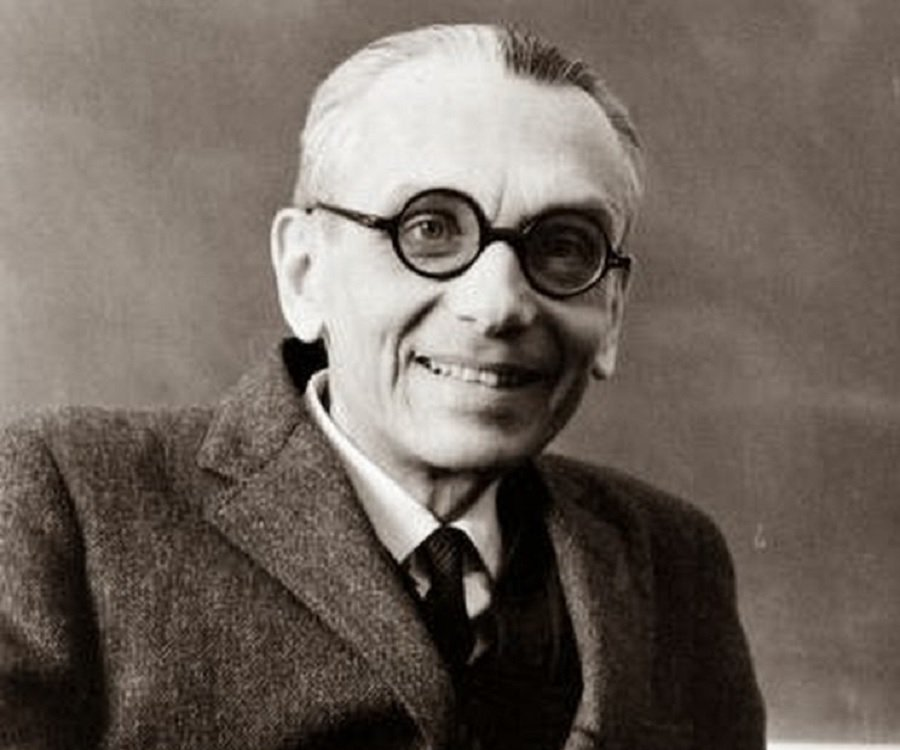
\includegraphics[width=.3\textwidth]{background/godel.jpg}
% % \end{center}

% Consider the following variant of the \HP, the Consistent Guessing Problem
% Given as input a description of a Turing machine $\TM$:
% if the machine $\TM$ accepts on a blank tape, then accept,
% if $\TM$ rejects on a blank tape, then reject, and
% if $TM$ runs forever on a blank tape, then either accept or reject,
% but in any case, halt!

% \margingraphic[l]{0.18\textwidth}{background/pix/rosser.png}{% https://www.math.cornell.edu/m/node/6955
%   \label{fig:rosser}\href{https://en.wikipedia.org/wiki/J._Barkley_Rosser}{J.\@ Barkley Rosser 1987--1989}} % https://www.math.cornell.edu/m/node/6955
% There is no Turing machine to solve the Consistent Guessing Problem.
% Let $P$ be a Turing machine that solves the Consistent Guessing Problem.
% Then we can easily modify $P$ to produce an new Turing machine $Q$ that,
% given as input a description $<\TM>$ of another Turing machine $\TM$:
% rejects if $TM(<\TM>)$ accepts,
% accepts if $\TM<\TM>$ rejects, and
% halts (either accepting or rejecting) if $\TM<\TM>$ runs forever.
% Now run $Q$ on its own description $Q<Q>$.
% If $Q<Q>$ accepts then it rejects; if $Q<Q>$ rejects, then it accepts.
% So the only remaining option is that $Q<Q>$ runs forever, violating the
% third condition.

% From the unsolvability of the Consistent Guessing Problem,
% I claim that Rosser’s Theorem follows.
% For suppose we had a complete and consistent (but not necessarily sound!)
% formal system $F$,
% which was powerful enough to talk about Turing machines.
% Then using $F$ we could solve the Consistent Guessing Problem as follows.
% Given as input a Turing machine description $<\TM>$,
% start enumerating all possible proofs and disproofs of the statement
% ``$\TM$ accepts on a blank tape.''
% Accept as soon as you find a proof, or reject as soon as you find a disproof.

% Because $F$ is complete, you must eventually find either a proof or a disproof
% (and therefore halt, either accepting or rejecting).
% Also, because $F$ is consistent,
% if $\TM$ really rejects then $F$ can't prove that $\TM$ accepts,
% while if $\TM$ really accepts then $F$ can't prove that
% $\TM$ doesn’t accept since in either case the contradiction could be
% discovered in finite time.
% So you'll accept if $\TM$ accepts and reject if $\TM$ rejects.
% But this means that you’re solving Consistent Guessing Problem.

% Just as a beginning programming class encourages a person to think that,
% once you are given a sufficiently detailed specificatino of the problem
% then producing a solution is routine, so also Hilbert and others perceived
% that we could produce an axiom system on which to base Mathematics.
% Then, for any question, with enough smarts we could settle any
% question at issue.

% The \HP{} shows that there are precisely stated problems that cannot be
% solved by an effective procedure.

% http://www.rudyrucker.com/blog/2012/08/01/memories-of-kurt-godel/

% The next form in which Zen expresses itself is the denial of opposites \ldots\,.
% The point is not to be `caught', as the masters would say, in any of the
% four propositions 1.~`It is A'; 2. `It is not-A'.;
% 3. `It is both A and not-A.';
% and 4.~`It is neither A nor not-A.'
% When we manke a negation or an assertion, we are sure to get into one of these
% logical formulas \ldots\,.
% It is in the nature of our logic that any statement we can make is so expressed.
% But Zen thinks that the truth can be reached when it is neither asserted nor
% negated.
% _Essays in Zen Buddhism_
% D.T.Suzuki
% 1949
% Grove Press p. 275



\part{Automata}
\chapteropen[\href{https://en.wikipedia.org/wiki/Automaton}{Automaton in the Swiss museum Centre International de la M\'ecanique d'Art, writing a letter.}]{automata/automaton.jpg}{Automata} %https://commons.wikimedia.org/wiki/File:CIMA_mg_8332.jpg
% License of photo: This work is free software; you can redistribute it or modify it under the terms of the CeCILL. The terms of the CeCILL license are available at www.cecill.info.

% Use as much of http://cstheory.stackexchange.com/a/14818/4731 as possible


\section{Finite state automata}

\subsection{Definition}


\subsection{Kleene's Theorem}

\subsection{Pumping}
Pumping Lemma

\subsection{Minimization}

Motivation

\begin{definition}
Let $\lang{L}$ be a language over an alphabet~$\Sigma$.
For a pair of strings $\sigma,\hat{\sigma}\in\kleenestar{\Sigma}$,
a \definend{distinguishing extension} is a 
string $\tau\in\kleenestar{\Sigma}$ 
such that exactly one of the two strings $\sigma\concat\tau$ 
and $\hat{\sigma}\concat\tau$ is an element of~$\lang{L}$. 
\end{definition}

Examples, including example where the two do not have a distinguishing 
extension.

\begin{definition}
Two strings $\sigma,\hat{\sigma}\in\kleenestar{\Sigma}$ are 
definend{$\lang{L}$-related}, written $\sigma\sim_{\lang{L}}\hat{\sigma}$,
if they have no distinguishing extension.  
\end{definition}

\begin{lemma}
For any language~$\lang{L}$,
the binary relation $\sim_{\lang{L}}$ between strings
is an equivalence relation.   
\end{lemma}

\begin{proof}
Sketch, including reminder of what is an equivalence.  
\end{proof}

Examples
Reminder of equivalence classes.

\begin{theorem}[Myhill-Nerode]
A language~$\lang{L}$ is regular if and only if the relation
$\sim_{\lang{L}}$ has only a finite number of equivalence classes.
\end{theorem}

Moreover, the proof will show that there is a correspondence between the classes
and the states of a finite state automata accepting that lanuguage.

\begin{proof}
Suppose that $\lang{L}$ is a regular, over the alphabet~$\Sigma$.
Then there is a finite state automata $\mathcal{A}$ accepting~$\lang{L}$.
Partition the set of all strings~$\kleenestar{\Sigma}$ with:
two strings $\sigma,\hat{\sigma}$ are in the same part if 
when~$\mathcal{A}$ is given them as input then they take 
the machine to the same state.
Observe that if two strings are in the same part then they are 
$\lang{L}$-related.
Thus, the parts are subsets of the equivalence classes of 
$\sim_{\lang{L}}$.
Since the number of parts is less than or equal to the number of states
in $\mathcal{A}$, the number of equivalence classes is finite.

If L is a regular language, then by definition there is a DFA A that recognizes it, with only finitely many states. If there are n states, then partition the set of all finite strings into n subsets, where subset Si is the set of strings that, when given as input to automaton A, cause it to end in state i. For every two strings x and y that belong to the same state, and for every choice of a third string z, automaton A reaches the same state on input xz as it reaches on input yz, and therefore must either accept both of the inputs xz and yz or reject both of them. Therefore, no string z can be a distinguishing extension for x and y, so they must be related by RL. Thus, Si is a subset of an equivalence class of RL. Combining this fact with the fact that every member of one of these equivalence classes belongs to one of the sets Si, this gives a many-to-one relation from states of A to equivalence classes, implying that the number of equivalence classes is finite and at most n.


\end{proof}

\section{Pushdown automata}

\subsection{Definition}

\extra{Neural nets}
\renewcommand{\asydir}{languages/asy/}


\begin{Filesave}{\answerbodyfilename}
  \def\asydir{languages/asy/} % Graphics from correct directory for this chapter
\end{Filesave}

% \chapteropen[\href{http://en.wikipedia.org/wiki/Plimpton_322}{Babylonian tablet, 1800~BCE, showing a set of Pythagorean triples.  The set of all such triples is a language of great interest.}]{languages/pix/plimpton322.png}{Languages}
\chapteropen[\href{https://en.wikipedia.org/wiki/Tower_of_Babel}{\textit{The Tower of Babel}, by Pieter Bruegel the Elder (1563)}]{languages/pix/babel.jpg}{语言、文法与图}
% https://upload.wikimedia.org/wikipedia/commons/5/50/Pieter_Bruegel_the_Elder_-_The_Tower_of_Babel_%28Vienna%29_-_Google_Art_Project.jpg
本章涵盖三个我们将在后续工作中用到的主题。

% https://github.com/stereobooster/programming-languages-genealogical-tree/blob/gh-pages/img/diagram-light.png

% ===============================================================
\section{语言}\index{language|(} % see for more: http://jeffe.cs.illinois.edu/teaching/algorithms/all-models.pdf
我们的机器输入和输出符号串。
我们将一个\definend{符号}，
有时也称为\definend{记号}，
视为机器可以读写的原子单元。\footnote{%
  我们可以想象 Turing 的计算员不读写符号进行计算，
  例如通过\protect\citetext{让大象走到路的左边或右边}{% 
    说得更实际一点，我们可能正在用乐高积木搭建一台 Turing 机，
    并想通过把一个积木块从柱子的一侧滑到另一侧来记录信息。
    或者，我们也可以用算盘。}来记录信息。
  但是，\protect\citetext{我们可以将任何此类过程转换}{%
    虽然一个人可能会合理地担心，大象不仅可以位于左边或右边，
    而是可以位于中间连续统中的任意一点，
    但我们只是基于我们机制的离散性（正如 Turing 基本上所做的那样）
    来做出这一断言，不做更多的哲学分析。
    也就是说，我们将其视为一条公理。}
  为使用我们机制的读写头能够处理的记号的过程。
  因此，可读性和可写性并非本质要求，
  但为了方便，我们在符号的定义中要求它们；毕竟，大象\emph{确实}不方便。}
在日常的二进制计算机上，符号是比特 \str{0} 和~\str{1}。
一个\definend{字母表}\index{alphabet}
是一个非空且有限的符号集合。
我们通常用大写希腊字母~$\Sigma$ 表示字母表，
不过比特字母表，即\definend{二元字母表 $\B=\set{\str{0},\str{1}}$}，是一个例外。
字母表上的一个\definend{串}\index{string}
是由该字母表中的符号组成的序列。
我们用小写希腊字母（如 $\sigma$ 和~$\tau$）表示串。
我们用 $\emptystring$ 表示空串，即长度为0的符号序列。
$\Sigma$ 上所有串的集合是
\index{Kleene star}$\kleenestar{\Sigma}$。\footnote{%
  关于串的更多内容见附录~\ref{sec:Strings}。}

%<*def:Lang>


\begin{definition}
一个\definend{字母表 $\Sigma$ 上的语言 $\lang$}\index{language}
是由该字母表上的串构成的集合。
即，$\lang\subseteq\kleenestar{\Sigma}\!$。
\end{definition}


%</def:Lang>

\begin{example}
以 \str{1} 开头的比特串集合是
$\lang=\set{\str{1},\,\str{10},\,\str{11},\,\str{100},\,\ldots}$。
\end{example}

\begin{example}
$\B$ 上的另一个语言是\citetext{有限集 $\set{\str{1000001},\str{1100001}}$}{%
  虽然看起来像是凭空挑出的两个串，但这个语言并非毫无意义。
  比特串 \str{1000001} 在 ASCII 编码中代表大写字母 A，
  而 \str{1100001} 代表小写字母 a。
  美国信息交换标准代码（ASCII）是一种在计算机中编码字符信息的
  广泛使用（尽管相当古老）的方法。
  现代最常用的字符编码是 UTF-8，它扩展了 ASCII。
  历史详情请见
  \url{https://www.cl.cam.ac.uk/~mgk25/ucs/utf-8-history.txt}。}。
\end{example}

\begin{example}
令 $\Sigma=\set{\str{a}, \str{b}}$。
由 \str{a} 的数量是 \str{b} 的数量两倍的串构成的语言是
$\lang=\set{\emptystring,\str{aab},\str{aba},\str{baa},
               \str{aaaabb}, \,\ldots}$。
\end{example}

\begin{example}
令 $\Sigma=\set{\str{a},\, \str{b},\, \str{c}}$。
该字母表上长度为2的串构成的语言是
$\lang_2=\Sigma^2=\set{\str{aa},\,\str{ab},\,\str{ba}\,\dots,\,\str{cc}}$。
在同一字母表上，下面这个语言由字符按升序排列的长度为3的串构成。
\begin{equation*}
  \lang_3=
  \set{\str{aaa},\,\str{bbb},\, \str{ccc},\, \str{aab},\, \str{aac},\, \str{abb},\, \str{abc},
    \str{acc},\,\str{bbc},\, \str{bcc}}
\end{equation*}
\end{example}

\begin{definition}\index{palindrome} \label{def:palindrome}
一个\citetext{\definend{回文}}{%
  有时人们称心理学是对大学新生的研究，因为许多研究大致是这样开头的：
  “我们把一群大学新生放进一个房间，就我们正在做的事情对他们撒谎，然后……”。
  同样地，计算理论有时也像是对回文的研究。}是正读与反读都相同的串。
\end{definition}

一些\citetext{英语中的回文}{%
  有些人喜欢超越单词回文的范畴，去构造有一定意义的句子长度的回文。
  一些较著名的例子有：(1)~据说是人类说出的第一句话，
  ``Madam, I'm Adam''（女士，我是亚当）；
  (2)~拿破仑的哀叹，``Able was I ere I saw Elba''（见到厄尔巴岛前，我无所不能）；
  以及 (3)~关于西奥多·罗斯福的 ``A man, a plan, a canal: Panama''（一个人，一个计划，一条运河：巴拿马）。
  另见 \url{http://norvig.com/palindrome.html}。}
有 \str{kayak}、\str{noon} 和~\str{racecar}。

\begin{example}
字母表 $\Sigma=\set{\str{a},\str{b}}$ 上的回文语言是
$\lang=\set{\sigma\in\kleenestar{\Sigma}\suchthat \sigma=\reversal{\sigma}}$。
其部分成员有 \str{abba}、\str{aaabaaa}、\str{a} 和 $\varepsilon$。
\end{example}

\begin{example}
令 $\Sigma=\set{\str{a}, \str{b}, \str{c}}$。
一组毕达哥拉斯整数三元组满足前两个数的平方和等于第三个数的平方，
例如 $3$、$4$、$5$ 或 $5$、$12$、$13$。
描述毕达哥拉斯三元组的一种方式是使用语言
$\lang
   = \set{\str{a}^i\str{b}^j\str{c}^k\in\kleenestar{\Sigma} 
            \suchthat \text{$i,j,k\in\N$ 且 $i^2+j^2=k^2$}}  
$。
一些成员是 $\str{aaabbbbccccc}=\str{a}^3\str{b}^4\str{c}^5\!$，
            $\str{a}^5\str{b}^{12}\str{c}^{13}\!$，以及
            $\str{a}^8\str{b}^{15}\str{c}^{17}\!$。
% \begin{align*}
%   \lang
%    &= \set{\str{a}^i\str{b}^j\str{c}^k\in\kleenestar{\Sigma} 
%             \suchthat \text{$i,j,k\in\N$ and $i^2+j^2=k^2$}}  \\
%    &=\set{\str{aaabbbbccccc}=\str{a}^3\str{b}^4\str{c}^5\!,\,
%             \str{a}^5\str{b}^{12}\str{c}^{13}\!,\,
%             \str{a}^8\str{b}^{15}\str{c}^{17}\!,\,\ldots}
% \end{align*}
\end{example}

\begin{example}
  空集是任意字母表上的一个语言 $\lang=\set{}$。
  仅含空串的集合 $\hat{\lang}=\set{\emptystring}$ 也是如此。
  这是两个不同的语言，因为第一个没有成员，而第二个有一个成员。
\end{example}

我们将“语言”定义为串集合的动机是：可以想象
$\Sigma$ 是词典中的单词集合，而句子是由单词构成的串。
然而，这样一来，语言可以是任意的单词串，
而在像英语这样的自然语言中，我们必须遵循规则。
下一节将研究语言的规则，即文法。

%<*def:class>


\begin{definition}
语言的汇集称为一个\definend{类}。\index{class!definition}\index{language!class, definition}
\end{definition}


%</def:class>

\begin{example}
对于任意字母表，该字母表上所有有限语言的汇集构成一个类。
\end{example}

% \begin{example}
% Another class is the collection of all languages over
% $\B=\kleenestar{\set{\str{0},\str{1}}}$ containing only
% strings with more \str{0}'s than \str{1}'s.
% One member of this class is the finite language
% $\lang_0=\set{\str{0},\str{001},\str{0001}}$.
% Another is $\lang_1=\set{\str{0}^{k+1}\str{1}^k\suchthat k\in\N}$.
% \end{example}

\begin{example}
令 $\TM_e$ 是一个使用输入字母表
$\Sigma=\set{\str{B},\str{1}}$ 的 Turing 机。
对于所有 $e\in\N$，串集合
$
W_e=\set{\sigma\in\kleenestar{\Sigma}\suchthat
  \text{$\TM_e$ 对输入 $\sigma$ 停机}}
$  is a language.
The collection of all such languages, of the $W_e$ 构成了 $\Sigma$ 上的可计算枚举语言类。
\end{example}

以下是作用于语言的自然运算。

%<*def:LangOps>


\begin{definition}[语言的运算]\index{language!operations on}  \label{def:LangOps}
\definend{语言拼接 $\lang_0\concat\lang_1$}
或 \definend{$\lang_0\lang_1$}\index{concatenation!of languages}\index{language!concatenation operation}，
是指所有拼接结果构成的语言，
$\set{\sigma_0\concat\sigma_1\suchthat \text{$\sigma_0\in\lang_0$ 且 $\sigma_1\in\lang_1$}}$。

对于任意语言 $\lang$，当 $k>0$ 时，
\definend{幂 $\smash{\lang^k}$}\index{power of a language}\index{language!power operation}
是由 $k$ 个成员拼接而成的语言，
$\smash{\lang^k}=
\set{\sigma_0\concat\cdots\concat\sigma_{k-1}\suchthat \sigma_i\in\lang}$。\footnotemark[1]
我们规定
$\smash{\lang^0}=\set{\emptystring}$。\footnotemark[2]
语言的
\definend{Kleene 星 $\smash{\kleenestar{\lang}}$}\index{Kleene star}\index{language!Kleene star operation}
是由任意多个串拼接而成的语言。
\begin{equation*}
\kleenestar{\lang}
  =\set{\sigma_0\concat\cdots\concat\sigma_{k-1}\suchthat \text{$k\in\N$ 且 $\sigma_0,\ldots,\sigma_{k-1}\in\lang$}}
  =\lang^0\cup\lang^1\cup\lang^2\cup\cdots
\end{equation*}
这包括 $0$ 个串的拼接，
因此 $\emptystring\in\kleenestar{\lang}$。\footnotemark[3]
语言的
\definend{反转}\index{reversal!of a language}\index{language!reversal operation}
是所有反转结果构成的语言，
$\smash{\reversal{\lang}}=\set{\smash{\reversal{\sigma}}\suchthat \sigma\in\lang}$。
\end{definition}

\footnotetext[1]{%
  请勿将此与集合的笛卡尔积运算混淆。
}%
\footnotetext[2]{%
  % We take $\lang^0=\set{\emptystring}$ even when
  % $\lang=\emptyset$.
  我们规定 $\sigma^0=\emptystring$，因为
  $\emptystring$ 是串拼接的幺元。
  （我们在第\pageref{page:PrimitiveRecursion}页将零个数的和定义为 $0$、零个数的积定义为 $1$ 时，
  也看到了同样的推理。）
  % Also see \zcref{exer:WhyEmptysetZeroPowerNotEmpty}.
}%
\footnotetext[3]{%
   即使 $\lang=\emptyset$，此结论也成立。
}

%</def:LangOps>

如\zcref{sec:Strings}所述，
我们将星号记号从语言扩展到字母表 $\Sigma$，
\citetext{定义 $\kleenestar{\Sigma}$
为由该字母表中的字符构成的所有串的集合}{%
  也就是说，我们不会刻意区分
  字母表中的符号和仅由这些符号构成的单字符串。}。\index{Kleene star}\index{alphabet!Kleene star}

\begin{example}
若该语言为比特串集合 $\lang=\set{\str{1000001},\str{1100001}}$，
则其反转为 $\reversal{\lang}=\set{\str{1000001},\str{10000011}}$。
\end{example}

%<*ex:KleeneStar>

\begin{example}
如果语言 $\lang$ 由两个串 $\set{\str{a},\,\str{bc}}$ 组成，
那么它的二次幂是
$\lang^2=\set{\str{aa},\,\str{abc},\,\str{bca},\,\str{bcbc}}$。
它的 Kleene 星是各次幂的并集。
\begin{equation*}
  \kleenestar{\lang}=\set{\emptystring,\,\str{a},\,\str{bc},\,\str{aa},\,\str{abc},\,\str{bca},\,\str{bcbc},\,\str{aaa},\,\ldots}  
\end{equation*}
\end{example}


%</ex:KleeneStar>

\begin{remark}
对于上述重复选择串的运算 $\lang^k$ 的定义，我们有两种可能的方式。
我们可以先选定一个串~$\sigma$，然后重复它，从而得到所有 $\sigma^k\!$ 的集合。
或者，我们可以重复地选择串，得到所有
$\sigma_0\concat\sigma_1\concat\cdots\concat\sigma_{k-1}$ 的集合。
第二种方式更有用，所以我们采用它。
\end{remark}

\label{discuss:LanguageDecidesRecognizes}
最后，我们描述机器与语言相关的两种方式。\footnote{%
  我们在定义~I.\protect\ref{df:TMDecidesLanguage}中针对一般集合讨论过这些运算，
  但这里我们针对语言这一特殊情况再重述一遍。}
%<*discussion:DecidingVsRecognizing>


\begin{definition} \label{def:MachineDecidesLanguage}
一台机器
\definend{判定一个语言（decides a language）}\index{decide a language}\index{language!decided by}，
是指它能计算出给定的输入是否属于该语言。
一台机器
\definend{识别（recognizes）}\index{recognized language}\index{language!recognized by}
% (or \definend{accepts},\index{accept a language}\index{language!accept} 
或 \definend{半判定（semidecides）}\index{semidecide a language}
一个语言，是指：若输入属于该语言，则机器在有限时间内计算出该结论；
若输入不属于该语言，则机器永远不会错误地报告其属于该语言。
\end{definition}

因此，如果一个语言~$\lang$ 不可计算，
那么就没有机器能判定它。
但如果 $\lang$ 是可计算枚举的，
那么就存在一台机器识别它。
若输入属于 $\lang$，这台机器可以在有限时间内计算出该结论；
但没有机器能在有限时间内确认其非成员资格。
可能存在一台机器能正确报告某些非成员的情况，但它必然在其他非成员上失败。
% because this language is not computable,
% no machine can determine on one hundred percent of inputs both
% membership and non-membership.
%</discussion:DecidingVsRecognizing>

简而言之，“判定”意味着机器对任何输入都能正确计算出所有肯定与否定的答案，
而“识别”是更弱的条件，只要求机器正确计算出所有肯定的答案。
% A language decider is a recognizer but the converse need not hold.  

%.....................................
\begin{exercises}


\begin{exercise}
列出每个语言中最短的五个串（如果有五个的话）。
\begin{exparts}
\item $\set{\sigma\in\kleenestar{\B}\suchthat
                    \text{$\str{0}$ 的数量与 $\str{1}$ 的数量之和等于 $3$}}$
\item $\set{\sigma\in\kleenestar{\B}\suchthat
             \text{$\sigma$ 的首字符与尾字符相同}}$
\end{exparts}
\begin{answer}\verified
\begin{exparts}
\item 五个串是：\str{000}、\str{001}、\str{010}、\str{011} 和~\str{100}。
\item 这五个满足条件：\str{0}、\str{1}、\str{00}、\str{11} 和~\str{000}。
  （空串属于这个语言吗？这可能存在争议，但可以肯定的是，空串的首尾字符并不不同。）
\end{exparts} 
\end{answer}
\end{exercise}

\recommended


\begin{exercise}
实数的十进制表示构成的集合是一个语言吗？
\begin{answer}\verified
不是。
根据定义，语言是串的集合，而根据定义，串的长度是有限的。
对于一些实数，其十进制表示不能构成有限长的串；
例如 $\pi=3.14\ldots$，再比如 $1/3=0.33\ldots$。
\end{answer}
\end{exercise}

\begin{exercise}
  以下哪个是回文：\str{()()} 还是 \str{)(()}？
  \begin{exparts*}
  \item 只有第一个
  \item 只有第二个
  \item 两个都是
  \item 两个都不是
  \end{exparts*}
\begin{answer}
  两个都是。
\end{answer}
\end{exercise}

\recommended


\begin{exercise}
证明：如果 $\beta$ 是一个串，那么 $\beta\concat\reversal{\beta}$ 是一个回文。
所有回文都具有这种形式吗？  
\begin{answer}\verified
  如果 $\beta=\sequence{b_0,\ldots,b_{i-1}}$ 是一个串，那么
  $\beta\concat\reversal{\beta}
  =\sequence{b_0,\ldots,b_{i-1}}\concat\sequence{b_{i-1},\ldots,b_0}$
  显然是一个回文。
  （这对空串也成立。）
  存在不是这种形式的回文。
  例如 $\gamma=\str{010}$，它不能分解为 $\gamma=\beta\concat\reversal{\beta}$，
  因为它的长度是奇数。
\end{answer}
\end{exercise}

\recommended


\begin{exercise}
令 $\lang_0=\set{\emptystring,\str{a},\str{aa},\str{aaa}}$ 和
$\lang_1=\set{\emptystring,\str{b},\str{bb},\str{bbb}}$。
\begin{exparts*}
\item 列出 $\lang_0\concat\lang_1$ 的所有成员。
\item 列出 $\lang_1\concat\lang_0$ 的所有成员。
\item 列出 $\lang_0^2$ 的所有成员。
\item 如果存在十个，列出 $\kleenestar{\lang_0\!}\!$ 的十个成员。
\end{exparts*}
\begin{answer}\verified
  \begin{exparts}
  \item 这些是 $\lang_0\concat\lang_1$ 的成员，
  其中第一行的串以空串开头，
  第二行的串以单个~\str{a} 开头，依此类推。
  \begin{align*}
    &\emptystring,\str{b},\str{bb},\str{bbb},  \\
    &\quad \str{a},\str{ab},\str{abb},\str{abbb} \\
    &\quad \str{aa},\str{aab},\str{aabb},\str{aabbb} \\
    &\quad \str{aaa},\str{aaab},\str{aaabb},\str{aaabbb} 
  \end{align*}
  \item 这些是 $\lang_1\concat\lang_0$ 的成员。
  \begin{align*}
    &\emptystring,\str{a},\str{aa},\str{aaa},  \\
    &\quad \str{b},\str{ba},\str{baa},\str{baaa} \\
    &\quad \str{bb},\str{bba},\str{bbaa},\str{bbaaa} \\
    &\quad \str{bbb},\str{bbba},\str{bbbaa},\str{bbbaaa} 
  \end{align*}
  \item 我们有如下结果。
  \begin{equation*}
    \lang_0^2=\lang_0\concat\lang_0=
      \set{\emptyset,\str{a},\str{aa},\str{aaa},\str{aaaa},\str{aaaaa},\str{aaaaaa}}
  \end{equation*}
  \item 正确答案有很多，但最自然的一组十个成员是：$\emptystring$、\str{a}、\str{aa}、……、$\str{a}^9\!$。 
  \end{exparts}
\end{answer}
\end{exercise}

\recommended


\begin{exercise}
列出下列每个语言的五个成员（如果有五个话）；如果不足五个，则列出所有成员。
\begin{exparts}
\item $\set{\sigma\in\kleenestar{\set{a,b}}\suchthat
              \text{$\sigma=\str{a}^n\str{b}$，其中 $n\in\N$}}$
\item $\set{\sigma\in\kleenestar{\set{a,b}}\suchthat
              \text{$\sigma=\str{a}^n\str{b}^n$，其中 $n\in\N$}}$
\item $\set{\str{1}^n\str{0}^{n+1}\in\kleenestar{\B}\suchthat
              n\in\N}$
\item $\set{\str{1}^n\str{0}^{2n}\str{1}\in\kleenestar{\B}\suchthat
              n\in\N}$
\end{exparts}
\begin{answer}\verified
  \begin{exparts}
  \item 该语言由任意多个 \str{a} 后接单个 \str{b} 构成。
    因此五个成员是 \str{b}、\str{ab}、\str{aab}、\str{aaab} 
    和~\str{aaaab}。
  \item 该语言由若干个 \str{a} 后接相同数量的 \str{b} 构成。
    因此五个成员是 \emptystring、\str{ab}、\str{aabb}、\str{aaabbb} 
    和~\str{aaaabbbb}。
  \item 该语言是由一串 \str{1} 后接一串 \str{0} 构成的串的集合，其中 \str{0} 的数量比 \str{1} 的数量多一。
    五个成员是
    \str{0}、\str{100}、\str{11000}、\str{1110000} 和~\str{111100000}。
  \item 该语言由 $\kleenestar{\B}$ 中的串构成，这些串先是一串 \str{1}，接着是一串 \str{0}，最后是一个 \str{1}。
    其中，\str{0} 的数量是前导 \str{1} 数量的两倍。 
    五个成员是
    \str{1}、\str{1001}、\str{1100001}、$\str{1}^3\str{0}^6\str{1}$,
    和~$\str{1}^4\str{0}^8\str{1}$。
  \end{exparts}
\end{answer}
\end{exercise}

\recommended


\begin{exercise}
已知 $\lang=\set{\str{a},\str{ab}}$，请分别列出以下各项。
\begin{exparts*}
\item $\lang^2$
\item $\lang^3$
\item $\lang^1$
\item $\lang^0$
\end{exparts*}
\begin{answer}\verified
  \begin{exparts}
  \item $\lang^2=\set{\str{aa},\str{aab},\str{aba},\str{abab}}$
  \item 我们先将集合中加入以 \str{aa} 开头的串，然后是以 \str{aab} 开头的串，以此类推。
    结果是 $\lang^3=\set{\str{aaa},\str{aaab},
                      \str{aaba},\str{aabab},
                      \str{abaa},\str{abaab},
                      \str{ababa},\str{ababab}}$.
  \item $\lang^1=\lang=\set{\str{a},\str{ab}}$
  \item $\lang^0=\set{\emptystring}$
  \end{exparts}
\end{answer}
\end{exercise}

\begin{exercise}
已知 $\lang_0=\set{\str{a},\str{ab}}$ 与 $\lang_1=\set{\str{b},\str{bb}}$，请分别求出以下各项。
\begin{exparts*}
\item $\lang_0\concat\lang_1$
\item $\lang_1\concat\lang_0$
\item $\lang_0^2$
\item $\lang_1^2$
\item $\lang_0^2\concat\lang_1^2$
% \item $\lang_1^2\concat\lang_0^2$
\end{exparts*}
\begin{answer}\verified
  \begin{exparts}
  \item $\lang_0\concat\lang_1=\set{\str{ab}, \str{abb}, \str{abb}, \str{abbb}}$
  \item $\lang_1\concat\lang_0=\set{\str{ba}, \str{bab}, \str{bba}, \str{bbab}}$
  \item $\lang_0^2=\set{\str{aa}, \str{aab}, \str{aba}, \str{abab}}$
  \item $\lang_1^2=\set{\str{bb}, \str{bbb}, \str{bbbb}}$
  \item $\lang_0^2\concat\lang_1^2=\set{\str{aabb}, \str{aabbb}, \str{aabbbb},
                                      \str{aabbbbb},
                                      \str{ababb}, \str{ababbb}, \str{ababbbb},\
                                      \str{ababbbbb}}$
  \end{exparts}
\end{answer}
\end{exercise}

\begin{exercise}
\begin{credit}
  F Stephan, \url{https://www.comp.nus.edu.sg/~fstephan/toc01slides.pdf}
\end{credit}
假设语言 $\lang_0$ 有三个元素，$\lang_1$ 有两个元素。
仅凭这一信息，求出下列各运算结果中元素数量的最小可能值和最大可能值。
\begin{exparts*}
\item $\lang_0\cup \lang_1$
\item $\lang_0\cap \lang_1$
\item $\lang_0\concat\lang_1$
\item $\lang_1^2$
\item $\reversal{\lang_1}$
\item $\kleenestar{\lang_0}\cap\kleenestar{\lang_1}$
\end{exparts*}
\begin{answer}\verified
\begin{exparts}
\item 
最小可能值是三，当 $\lang_1$ 是 $\lang_0$ 的子集时取到。
最大可能值是五，当两个语言互不相交时取到。
\item
最小可能值是零，当两个语言互不相交时取到。
最大可能值是二，当 $\lang_1$ 是 $\lang_0$ 的子集时取到。
\item 
最大可能值是六，例如当
$\lang_0=\set{\str{a},\str{b},\str{c}}$ 且 $\lang_1=\set{\str{x},\str{y}}$ 时，
得到 
$\lang_0\concat\lang_1=\set{\str{ax},\str{ay},\str{bx},\str{by},\str{cx},\str{cy}}$。
最小可能值是四，例如当
$\lang_0=\set{\emptystring,\str{a},\str{aa}}$ 且 
$\lang_1=\set{\emptystring,\str{a}}$ 时，得到
$\lang_0\concat\lang_1=\set{\emptystring,\str{a},\str{aa},\str{aaa}}$。
\item
最小可能值是三，例如当 $\lang_1=\set{\emptystring,\str{a}}$ 时，
得到 $\lang_1^2=\set{\emptystring,\str{a},\str{aa}}$。
最大可能值是四，例如当 
$\lang_1=\set{\str{a},\str{b}}$ 时，得到
$\lang_1^2=\set{\str{aa},\str{ab},\str{ba},\str{bb}}$。
\item
唯一可能的数量是 $2$。 
$\lang_1$ 中的两个元素反转后不可能成为同一个元素，否则它们在反转前就是同一个元素了。
（即使其中一个元素是空串，此结论也成立。）
\item
交集可以是无限的，例如当 
$\lang_0=\set{\emptystring,\str{a},\str{b}}$ 且
$\lang_1=\set{\emptystring,\str{a}}$ 时，
其中 $\str{a}^n\in\kleenestar{\lang_0}\cap\kleenestar{\lang_1}$ 对所有的 $n\in\N$ 都成立。
交集的大小最小可以是 $1$，例如当
$\lang_0=\set{\str{a},\str{b},\str{c}}$ 且 
$\lang_1=\set{\str{x},\str{y}}$ 时，
此时 $\kleenestar{\lang_0}\cap\kleenestar{\lang_1}$ 的唯一元素是空串。
\end{exparts}
\end{answer}
\end{exercise}

% \begin{exercise}
% Let $\lang=\set{\str{a},\str{b}}$.
% Why is $\lang^0$ defined to be $\set{\emptystring}$?
% Why not $\emptyset$?
% \begin{answer}\verified
%   The concatenation of $0$-many strings is $\emptystring$.
%   That is, if $\sigma\in\lang$ then $\sigma^0$ is defined to be the 
%   empty string.
% \end{answer}
% \end{exercise}

\begin{exercise}
空集的 Kleene 星，即 $\kleenestar{\emptyset}$，是什么样的语言？
\begin{answer}\verified
  它是空集，即 $\kleenestar{\emptyset}=\emptyset$。
  根据定义， 
  $\kleenestar{\lang}=\set{\sigma_0\concat\cdots\concat\sigma_{k-1}\suchthat \text{$k\in\N$ 且 $\sigma_0,\ldots,\sigma_{k-1}\in\lang$}}$。
  如果该语言为空，那么“$\sigma_0,\ldots,\sigma_{k-1}\in\lang$”这一条件永远无法满足。
\end{answer}
\end{exercise}

\recommended

\begin{exercise}
一个语言的 $k$ 次幂是否等同于由 $k$ 次幂组成的语言？   
\begin{answer}\verified
  不相等。
  设 $\lang=\set{\str{a}, \str{b}}$ 并设 $k=2$。
  那么该语言的 $2$ 次幂是
  $\lang^k=\set{\str{aa},\,\str{ab},\,\str{ba},\,\str{bb}}$，而  
  由 $2$ 次幂组成的语言是
  $\set{\sigma^2\suchthat \sigma\in\lang}=\set{\str{aa},\,\str{bb}}$。
\end{answer}
\end{exercise}

% \begin{exercise}
% Show that the set of languages for which there is a Turing machine that
% accepts it is countable.
% (We will say that a Turing machine accepts a string if when started 
% with that string as the only thing on the tape, and with the head under the 
% leftmost character of the string, the machine halts and outputs~\str{1}.)
% Show that it is not effectively countable\Dash there is no effective
% one to one and onto function from $\N$ to this set.
% \end{exercise}

\begin{exercise}
$\kleenestar{\lang}$ 是否不同于 
$\kleenestar{(\lang\cup\set{\emptystring})}$？
\begin{answer}\verified
  是，但仅在一个边界情形下不同。
  如果 $\lang=\emptyset$，那么 $\kleenestar{\lang}=\emptyset$，
  而 $\kleenestar{(\lang\cup\set{\emptystring})}=\set{\emptystring}$。

  我们将证明，如果 $\lang\neq\emptyset$，那么这两个集合相等，
  即 $\kleenestar{\lang}=\kleenestar{(\lang\cup\set{\emptystring})}\!$。
  包含关系 
  $\kleenestar{\lang}\subseteq\kleenestar{(\lang\cup\set{\emptystring})}$
  是显然的。

  对于另一个方向，即要证 
  $\kleenestar{(\lang\cup\set{\emptystring})}\subseteq\kleenestar{\lang}$，
  假设 $\sigma\in\kleenestar{(\lang\cup\set{\emptystring})}\!$，其中
  $\sigma=\sigma_0\concat\cdots\concat\sigma_{n-1}$ 对某个 $n\in\N$ 成立，且
  所有的 $\sigma_i$ 都是 $\lang\cup\set{\emptystring}$ 中的元素。
  如果对所有 $i\in\set{0,\ldots n-1}$ 都有串 $\sigma_i$ 
  等于 $\emptystring$，那么 $\sigma=\emptystring$，并且它属于
  $\kleenestar{\lang}$，因为 $\lang\neq\emptyset$ 且
  对任意 $\rho\in\lang$ 都有 $\emptystring=\rho^0$。
  否则，至少存在一个 $i\in\set{0,\ldots n-1}$ 
  使得 $\sigma_i\neq\emptystring$。
  在这种情况下，从串 $\sigma$ 中去掉那些等于空串的 $\sigma_j$，
  可得对某个 $k\leq n$ 有 $\sigma\in\lang^k$，
  因此 $\sigma\in\kleenestar{\lang}\!$。  
\end{answer}
\end{exercise}

\begin{exercise}
我们可以考虑集合 $\lang^2\!$ 中有多少个元素。
\begin{exparts}
\item 证明如果两个串不相等，那么它们的平方也不相等。  
  并由此得出结论：若 $\lang$ 有 $k$ 个元素，则
  $\lang^2$ 至少有 $k$ 个元素。
\item 举一个非空语言的例子，使其元素的个数恰好等于这个下界。
\item 证明若 $\lang$ 有 $k$ 个元素，则 $\lang^2$ 至多有
$k^2$ 个元素。
\item 对于每个 $k\in\N$，举一个语言的例子，使其平方达到这个上界。 
\end{exparts}
\begin{answer}\verified
  对任意语言，我们记其字母表为 $\Sigma$。
  \begin{exparts}
  \item 考虑两个不相等的串 $\sigma_0\neq\sigma_1$。
    它们不可能都是空串；如果其中一个是空串而另一个不是，
    那么显然 $\sigma_0^2\neq\sigma_1^2$，
    因为这两个平方中有一个是空串而另一个不是。
    现在假设 $\sigma_0$ 和 $\sigma_1$ 都不是空串。
    如果它们长度不同，那么它们的平方长度也不同。
    剩下的情况是它们为非空且等长的串，
    即 $\sigma_0=\sequence{s_{0,0},s_{0,1},\ldots\, s_{0,n}}$
    且
    $\sigma_1=\sequence{s_{1,0},s_{1,1},\ldots\, s_{1,n}}$ 对某个 $n\in\N$ 成立。
    取定最小的索引 $i$ 使得 $s_{0,i}\neq s_{1,i}$。
    对于这个相同的 $i$，$\sigma_0^2$ 和 $\sigma_1^2$ 在第 $i$ 个位置不同，
    因此它们不相等。

    上一段表明，如果 $\lang$ 有 $k$ 个不同的元素
    $\lang=\set{\sigma_0,\ldots \sigma_{k-1}}$，那么串
    $\sigma_0^2$,\ldots, $\sigma_{k-1}^2$ 互不相同，因此
    $\lang^2$ 至少有 $k$ 个不同的元素。
  \item 语言 $\lang=\set{\emptystring}$ 满足
    $\lang^2=\set{\emptystring}$。
  \item 设 $\lang=\set{\sigma_0,\sigma_1,\ldots\, \sigma_{k-1}}$，其中 $k\in\N^+$ 
    （我们假定这些串彼此互不相同）。
    那么列表
    $\sigma_0\concat\sigma_0$, $\sigma_0\concat\sigma_1$,
    \ldots{} $\sigma_{k-1}\concat\sigma_{k-1}$ 的长度为 $k^2\!$。
    因此，$\lang^2$ 可能具有的最大元素个数是 $k^2\!$。
  \item 考虑语言 
    $\lang=\set{\sigma_0, \sigma_1,\ldots\, \sigma_{k-1}}$，
    其中这 $k$ 个串长度均为 $1$ 且互不相等，
    因此每个串由单个符号组成，且其使用的符号与任何其他串所使用的符号都不相同。
    显然，列表 
    $\sigma_0\concat\sigma_0$, $\sigma_0\concat\sigma_1$,
    \ldots{} $\sigma_{k-1}\concat\sigma_{k-1}$
    中的所有成员都互不相同，所以 $\lang^2$ 有 $k^2$ 个元素。
  \end{exparts}
\end{answer}
\end{exercise}

\begin{exercise}
证明 $\kleenestar{\lang}=\lang^0\union\lang^1\union\lang^2\union\cdots\,$。
\begin{answer}\verified
  回顾 $\lang^k=
  \set{\sigma_0\concat\cdots\concat\sigma_{k-1}\suchthat \sigma_i\in\lang}$
  以及 $\kleenestar{\lang}=\set{\sigma_0\concat\cdots\concat\sigma_{k-1}\suchthat \text{$k\in\N$ 且 $\sigma_0,\ldots,\sigma_{k-1}\in\lang$}}$。
  如果 $\lang=\emptyset$，那么根据定义有 $\kleenestar{\lang}=\set{\emptystring}$。
  如果 $\lang=\emptyset$，那么根据定义有 $\lang^0=\set{\emptystring}$，
  而对任意 $k> 0$，都有 $\lang^k=\emptyset$。

  因此剩下的就是论证 $\lang\neq\emptyset$ 的情况。
  我们先证明 $\lang^k\subseteq\kleenestar{\lang}\!$。
  如果 $k=0$，因为我们假设 $\lang\neq\emptyset$，可以取 $\sigma\in\lang$，则有 $\sigma^0=\emptystring$。
  因此 $\lang^0=\set{\emptystring}$ 且 $\emptystring\in\kleenestar{\lang}\!$。
  现在假设 $k>0$，并取定 $\sigma\in\lang^k$，满足 $\sigma=\sigma_0\concat\cdots\concat\sigma_{k-1}$。
  那么根据 $\kleenestar{\lang}$ 的定义，有 $\sigma\in\kleenestar{\lang}$。

  最后我们证明 $\kleenestar{\lang}\subseteq\lang^0\cup\lang^1\cup\cdots$。
  取定 $\sigma\in\kleenestar{\lang}$（注意 $\lang\neq\emptyset$），
  于是存在某个 $k\in\N$ 使得 $\sigma=\sigma_0\concat\cdots\concat\sigma_{k-1}$。
  注意 $\sigma\in\lang^k$（即使 $k=0$ 也成立）。
  因此 $\kleenestar{\lang}\subseteq\lang^0\cup\lang^1\cup\cdots\,$。
\end{answer}
\end{exercise}

\begin{exercise}
考虑空语言 $\lang_0=\emptyset$。
对任意语言 $\lang_1$，描述 $\lang_1\concat\lang_0$。
\begin{answer}\verified
所有形如 $\sigma_1\concat\sigma_0$（其中 $\sigma_1\in\lang_1$ 且 $\sigma_0\in\lang_0$）的拼接所构成的集合是空集，
因为 $\lang_0$ 中不存在成员 $\sigma_0$。
\end{answer}
\end{exercise}

\begin{exercise} \label{exer:LanguageUnionIntersection}
语言是集合，因此可以应用并集和交集运算。
\begin{exparts}
\item
写出 $A=\kleenestar{\set{\str{a}}}$ 与 $B=\kleenestar{\set{\str{b}}}\!$ 的并集中最短的五个串。
\item
假设 $\Sigma_0$ 和 $\Sigma_1$ 不相交，并且 $\lang_0$ 和 $\lang_1$ 分别是定义在这两个字母表上的有限语言。
它们的并集有多少个元素？
\item 填空：一个在 $\Sigma_0$ 上的语言与一个在 $\Sigma_1$ 上的语言的并集，是一个在 \fillinblank{} 上的语言。
\item 为交集写出类似的陈述。    
\end{exparts}
\begin{answer}\verified
\begin{exparts}
\item 它们是 $\emptystring$、\str{a}、\str{aa}、\str{b} 以及 \str{bb}。
\item 并集的元素个数等于第一个语言的元素个数加上第二个语言的元素个数。
因为字母表不相交，所以两个语言之间没有重叠。    
\item
并集中的串可能包含来自任一字母表的字符。
因此，一个在 $\Sigma_0$ 上的语言与一个在 $\Sigma_1$ 上的语言的并集，是一个在 $\Sigma_0\cup\Sigma_1$ 上的语言。
\item
要属于这两个语言的交集，一个串必须只包含同时属于这两个字母表的字符。
因此，一个在 $\Sigma_0$ 上的语言与一个在 $\Sigma_1$ 上的语言的交集，是一个在 $\Sigma_0\cap\Sigma_1$ 上的语言。
\end{exparts}
\end{answer}
\end{exercise}

\begin{exercise}
设字母表 $\Sigma$ 上的语言~$\lang$ 是有限的，即假设 $\lh{\lang}<\infty$。
\begin{exparts}
\item 若语言有限，字母表必须有限吗？
\item 证明存在某个 $B\in\N$，使得对所有 $\sigma\in\lang$ 有 $\lh{\sigma}\leq B$。
\item 证明有限语言类在有限并下封闭。
  即，证明如果 $\lang_0,\ldots\, \lang_{k-1}$ 是某个共享字母表上的有限语言（其中 $k\in\N$），则它们的并也是有限的。
\item 同时证明有限语言类在有限交和有限拼接下封闭。
\item 证明有限语言类在补运算和 Kleene 星下不封闭。
  （对于字母表~$\Sigma$，语言是一个子集 $\lang\subseteq\kleenestar{\Sigma}$。
  所以其补集是 $\setcomp{\lang}=\kleenestar{\Sigma}-\lang$，\index{language!complement}\index{complement of a language} 也是 $\Sigma$ 上的语言。）
\end{exparts}
\begin{answer}\verified
  \begin{exparts}
  \item 是的，但这与语言有限无关。
    根据我们的定义，字母表是有限的。
    （\zcref{sec:Strings}有相关回顾。）
  \item 因为语言有限，要么语言为空，此时可取 $B=0$；要么语言中存在最长串，可取 $B$ 为该串的长度。
  \item 设 $\lang_0,\ldots\, \lang_{k-1}$ 是 $\kleenestar{\Sigma}$ 上的有限语言（$k\in\N$）。
    则它们的并也是有限的，因为它至多包含 $\lh{\lang_0}+\cdots+\lh{\lang_{k-1}}$ 个元素。
  \item 设 $\lang_0,\ldots\, \lang_{k-1}$ 是 $\kleenestar{\Sigma}$ 上的有限语言。
    则它们的交至多包含 $\min(\lh{\lang_0},\ldots \lh{\lang_{k-1}})$ 个元素，因此也是有限的。
    拼接 $\lang_0\concat\lang_1\concat\cdots\concat\lang_{k-1}$ 中的串数至多是乘积 $\lh{\lang_0}\cdot\lh{\lang_0}\cdots \lh{\lang_{k-1}}$。
  \item 如果 $\Sigma=\set{\str{a},\str{b}}$，则有限语言 $\lang=\set{}$ 的补集是 $\setcomp{\lang}=\kleenestar{\Sigma}\!$，它是无限的，因为它对所有 $n$ 都包含 $\str{a}^n$。
    对于同一字母表，$\lang=\set{\str{a},\str{b}}$ 是有限的，但 $\kleenestar{\lang}$ 是无限的。
  \end{exparts}
\end{answer}
\end{exercise}

\begin{exercise}
语言 $\lang 
    =\set{\sigma\in\kleenestar{\Sigma}\suchthat \sigma=\reversal{\sigma}}$ 和 $\hat{\lang} 
  =\set{\sigma\concat\reversal{\sigma}\suchthat \sigma\in\kleenestar{\Sigma}}$ 有什么区别？
\begin{answer}\verified
  在 $\hat{\lang}$ 中，所有串的长度均为偶数，因此它包含所有偶数长度的回文。
  语言 $\lang$ 则包含任意长度的所有回文。
\end{answer}
\end{exercise}

\begin{exercise}
对于任意语言 $\lang\subseteq\kleenestar{\Sigma}$，我们可以构成其前缀集合。
\begin{equation*} 
  \operatorname{Pref}(\lang)
   =\set{\tau\in\kleenestar{\Sigma}
         \suchthat\text{$\sigma\in\lang$ 且 $\tau$ 是 $\sigma$ 的前缀}}
\end{equation*}
若 $\Sigma=\set{\str{a},\str{b}}$ 且 $\lang=\set{\str{abaaba},\str{bba}}$，求 $\operatorname{Pref}(\lang)$。
\begin{answer}\verified
  前缀为 
  $\emptystring$, 
  $\str{a}$, $\str{b}$,
  $\str{ab}$, $\str{bb}$,
  $\str{aba}$, $\str{bba}$,
  $\str{abaa}$, 
  $\str{abaab}$,
  以及 
  $\str{abaaba}$。
\end{answer}
\end{exercise}

\begin{exercise} \label{exer:WhyEmptysetZeroPowerNotEmpty}
\begin{credit}
  \href{https://cs.stackexchange.com/a/44912/67754}{SE user babou}
\end{credit}
这解释了为什么即使 $\lang=\emptyset$，我们也定义 $\lang^0=\set{\emptystring}$。
\begin{exparts}
\item 证明对于任意 $m,n\in\N^+\!$，$\lang^m\,\concat\!\lang^n=\lang^{m+n}$。
\item 证明如果 $\lang_0=\emptyset$，则 $\lang_0\concat\lang_1=\lang_1\concat\lang_0=\emptyset$。
\item 论证如果 $\lang\neq\emptyset$，那么 $\lang^0$ 唯一合理的定义是 $\set{\emptystring}$。
\item 为什么若 $\lang=\emptyset$ 且不定义 $\lang^0=\set{\emptystring}$，就会导致问题？
\end{exparts}
\begin{answer}\verified
\begin{exparts}
\item 将 $\sigma_0\concat\cdots\concat\sigma_{m-1}\in\lang^m$ 与 $\tau_0\concat\cdots\concat\tau_{n-1}\in\lang^n$ 拼接得到 $\sigma_0\concat\cdots\concat\sigma_{m-1}\concat\tau_0\concat\cdots\concat\tau_{n-1}\in\lang^{m+n}$。
\item 根据定义，$\lang_0\concat\lang_1
  =\set{\sigma_0\concat\sigma_1\suchthat 
        \text{$\sigma_0\in\lang_0$ 且 $\sigma_1\in\lang_1$}}$。
  如果两者之一是空集，则条件永远不满足，因此结果是空集。
\item 对于任意串 $\sigma\in\kleenestar{\lang}$，我们有 $\sigma^0=\emptystring$。
  因此，如果语言中有任何串，那么将它们取零次幂都会得到空串，所以结果是 $\lang^0=\set{\emptystring}$。
\item 如果 $\lang=\emptyset$ 会使得 $\lang^0=\emptyset$，那么对于任意语言~$\hat{\lang}$，
  扩展前一项的公式会得到 $\hat{\lang}=\hat{\lang}^{\,1}=\hat{\lang}^{\,1+0}
    =\hat{\lang}\concat\emptyset=\emptyset$（最后的等式由第二项得出），这是不合理的。
\end{exparts}
\end{answer}
\end{exercise}

\begin{exercise}
证明以下命题对任意字母表 $\Sigma$ 成立。
\begin{exparts}
\item 对于任意自然数~$n$，语言 $\Sigma^n$ 是可数的。
\item 语言 $\kleenestar{\Sigma}$ 是可数的。
\end{exparts}
\begin{answer}
  \begin{exparts}
  \item 考虑集合
    $S=\Sigma\times\cdots\times\Sigma$
    （我们避免将其称为 $\Sigma^n$，因为二者不同，
    笛卡尔积是 $n$ 元组的集合，而 $\Sigma^n$ 是 $\kleenestar{\Sigma}$ 的一个子集）。
    它是可数多个可数集的笛卡尔积，因此根据第二章的
    \zcref{cor:CrossProdCountablyManyIsCountable}，它是可数的。
    所以存在一一且满射的函数 $\map{g}{\N}{S}$。
    将其自变量拼接起来 $f(\sigma_0,\ldots \sigma_{n-1})=\sigma_0\concat\cdots\concat\sigma_{n-1}$ 的函数
    $\map{\operatorname{concat}}{S}{\Sigma^n}$
    显然也是满射的。
    因此复合 $\map{\composed{f}{g}}{\N}{\Sigma^n}$ 是满射的。
    那么根据第二章的\zcref{lem:CountableIffOntomap}，$\Sigma^n$ 是可数的。
  \item 集合 $\kleenestar{\Sigma}=\Sigma^0\cup\Sigma^1\cup\cdots\,$ 是可数多个可数集的并集，因此根据
    第二章的\zcref{th:UnionFiniteNumberCtbleSets}，它是一个可数集。
  \end{exparts}
\end{answer}
\end{exercise}

\begin{exercise}
  \zcref{def:LangOps}中对语言幂的描述写的是 $\sigma_0\concat\cdots\concat\sigma_{k-1}$，
  没有括号，因而未明确该集合的构造方式。
  自然的构造方式是：定义 $\lang^0=\set{\emptystring}$，
  以及 $\lang^{k+1}=\lang^k\concat\lang$。
  验证这种构造方式给出的集合与定义中的相同。
\begin{answer}\verified
  我们需要验证的是：对拼接运算任意两种加括号的方式都产生同一个串。
  为避免两种形式混淆，仅在此论证中将
  $\set{\sigma_0\concat\cdots\concat\sigma_{k-1}\suchthat \sigma_i\in\lang}$
  记作 ${}^k\!\lang\!$。

  我们首先证明 ${}^k\!\lang$ 的任何元素都是 $\lang^{k}\!$ 的元素。
  % so fix $\sigma=\sigma_0\concat\cdots\concat\sigma_{k-1}\in {}^k\lang$.
  我们进行一个简单的归纳论证。
  基础情形是：按定义，${}^0\!\lang$ 和 $\lang^0$ 都等于
  $\set{\emptystring}$；并且对于任何 $\sigma_0\in\lang$，有 $\sigma_0\in\lang^1$ 和 $\sigma_0\in{}^1\!\lang$。
  归纳假设是：
  $\sigma_0\concat\cdots\concat\sigma_{i-1}\in {}^i\!\lang$
  蕴含
  $\sigma_0\concat\cdots\concat\sigma_{i-1}\in\lang^i$，其中
  $i\in\set{0,\ldots\,j}$。
  对于 $i=j+1$ 的归纳步骤，假设我们有一个由 $j+1$ 个串构成的拼接：
  $\sigma_0\concat\cdots\concat\sigma_{j-1}\concat\sigma_j\in{}^{j+1}\!\lang$。
  应用串拼接运算的结合律将其重写为 $(\sigma_0\concat\cdots\concat\sigma_{j-1})\concat\sigma_j$，
  根据本练习中 $\lang^{j+1}$ 的定义，
  $(\sigma_0\concat\cdots\concat\sigma_{j-1})\concat\sigma_j\in\lang^{j+1}\!$。

  另一方向是：对于任意~$k$，$\lang^k$ 的任何元素都是
  ${}^k\!\lang$ 的元素。
  这里我们也用归纳法。
  同样地，$k=0$ 和 $k=1$ 的
  基础情形是：按定义，${}^0\!\lang$ 和 $\lang^0$ 等于
  $\set{\emptystring}$；并且对于任何 $\sigma_0\in\lang$，有 $\sigma_0\in\lang^1$ 和 $\sigma_0\in{}^1\!\lang$。
  归纳假设是：如果 $\sigma\in\lang^{i}$，那么
  $\sigma\in {}^{i}\!\lang$，其中 $i\in\set{0,\ldots\,k}$。
  $\lang^j$ 的任何元素都具有形式
  $(\sigma_0\concat\cdots\concat\sigma_{j-1})\concat\sigma_j$。
  利用串拼接的结合律，我们可以去掉括号将其写为
  $\sigma_0\concat\cdots\concat\sigma_{j-1}\concat\sigma_j$
  （更准确地说，任何加括号方式都给出相同的最终串），
  这是 ${}^{j+1}\lang$ 的一个元素。
\end{answer}
\end{exercise}

\begin{exercise}
判断真假：如果 $\lang\concat\lang=\lang$，那么要么 $\lang=\emptyset$，
要么 $\emptystring\in\lang$。
若为真则给出证明，若为假则给出反例。
\begin{answer}\verified
  命题为真。
  作为论证的启发，构造反例时自然会想到的语言是 $\lang=\set{\str{a},\str{aa}, \ldots{}}$。
  然而，$\lang\concat\lang$ 是~$\lang$ 的真子集，因为它不包含~$\str{a}$。

  于是，考虑 $\lang\neq\emptyset$ 的情况，目标是证明
  $\emptystring\in\lang$。
  该语言非空，因此至少包含一个元素。
  在所有这些串中，设最短的长度为~$\ell\in\N$。
  如果 $\ell>0$，那么 $\lang\concat\lang$ 的任何元素的长度至少为 $2\ell$，当 $\ell>0$ 时该长度严格大于
  $\ell$。
  但根据练习假设 $\lang\concat\lang=\lang$，
  由此产生矛盾。
  另一种可能性是 $\ell=0$，这意味着
  $\emptystring\in\lang$。
\end{answer}
\end{exercise}

\begin{exercise}
证明没有任何语言能包含每个实数的表示。
\begin{answer}\verified
每个语言都是可数的，因为它是 $\kleenestar{\Sigma}\!$ 的子集，
而根据字母表的定义 $\Sigma$ 是有限的，所以 $\kleenestar{\Sigma}$ 是可数的。
但实数有不可数多个。
\end{answer}
\end{exercise}

\begin{exercise}
语言运算构成一个代数系统。
假设这些语言都在同一个字母表上。
证明以下每条性质。
\begin{exparts}
\item 语言的并和交是交换的，
  $\lang_0\cup\lang_1=\lang_1\cup\lang_0$ 且
  $\lang_0\cap\lang_1=\lang_1\cap\lang_0$。
\item
仅由空串构成的语言是关于语言拼接的单位元，
即 $\lang\concat\set{\emptystring}=\lang$
且 $\set{\emptystring}\concat\lang=\lang$。
\item
语言拼接未必是交换的；
存在满足
$\lang_0\concat\lang_1\neq\lang_1\concat\lang_0$ 的语言。
\item
语言拼接是结合的，
$(\lang_0\concat\lang_1)\concat\lang_2
  =\lang_0\concat(\lang_1\concat\lang_2)$。
\item
$\reversal{(\lang_0\concat\lang_1)}
    =\reversal{\lang_1}\concat\reversal{\lang_0}\!$。
\item
拼接对并运算满足左分配律，
$(\lang_0\cup\lang_1)\concat\lang_2
 =(\lang_0\concat\lang_2)\,\cup\,(\lang_1\concat\lang_2)$，
并且也满足右分配律。
\item
空语言是拼接的零元，即 $\emptyset\concat\lang=\lang\concat\emptyset=\emptyset$。
\item Kleene 星运算是幂等的，
$\kleenestar{(\kleenestar{\lang})}=\kleenestar{\lang}\!$。
\end{exparts}
\begin{answer}\verified
\begin{exparts}
\item 对于任意集合，无论是否为语言，并和交都是交换的。
\item 我们有
  $\lang\concat\set{\emptystring}=\set{\sigma\concat\emptystring\suchthat \sigma\in\lang}=\set{\sigma\suchthat \sigma\in\lang}=\lang$。
\item 设 $\Sigma=\set{\str{a},\str{b}}$，
  取 $\lang_0$ 为单字符串集合 $\set{\str{a}}$，
  类似地令 $\lang_1=\set{\str{b}}$。
  那么 $\lang_0\concat\lang_1$ 也仅有单个串，即 $\set{\str{ab}}$，
  而
  $\lang_1\concat\lang_0=\set{\str{ba}}$。
\item 这可直接由串的拼接满足结合律得出：$(\sigma_0\concat\sigma_1)\concat\sigma_2$
  的第 $i$ 个元素与 $\sigma_0\concat(\sigma_1\concat\sigma_2)$ 的第 $i$ 个元素相同。
\item 这可直接由对于串，
  $\reversal{(\sigma_0\concat\sigma_1)}$ 等于
  $\reversal{\sigma_1}\concat\reversal{\sigma_0}\!$ 得出。
\item 一个串是 $(\lang_0\cup\lang_1)\concat\lang_2$ 的元素，
  当且仅当它具有 $\sigma\concat\tau$ 形式，其中
  $\tau\in\lang_2$，并且 $\sigma\in\lang_0$ 或 $\sigma\in\lang_1$。
  这成立，当且仅当 $\tau\in\lang_2$ 且 $\sigma\in\lang_0$，
  或者 $\tau\in\lang_2$ 且 $\sigma\in\lang_1$。
  而这又等价于
  $\sigma\in(\lang_0\concat\lang_2)\cup(\lang_1\concat\lang_2)$。
  右分配律的论证同理。
\item 对任意语言~$\lang$，其定义为
  $\emptyset\concat\lang=\set{\sigma_0\concat\sigma_1
    \suchthat \text{$\sigma_0\in\emptyset$ 且 $\sigma_1\in\lang$}}$。
  条件“$\sigma_0\in\emptyset$”永远无法满足，因此该集合为空。
  $\lang\concat\emptyset$ 同理。
\item 对于任意字符串，无论拼接如何加括号，都可以去掉括号。
  例如，$((\sigma_0\concat\sigma_1)\concat\sigma_2)\concat\sigma_3$
  等于 $((\sigma_0\concat(\sigma_1\concat\sigma_2))\concat\sigma_3$，
  因为两者的第 $i$ 个元素相等。
  （我们可以通过归纳法轻易证明该陈述。）
  由此可直接得出结论。
\end{exparts}
\end{answer}
\end{exercise}

\end{exercises}
\index{language|)}

% =====================================================
\section{文法}\index{grammar|(}  \label{sec:Grammars}
我们已把语言定义为串的集合。
但这允许任何杂乱无章的集合。
\citetext{实际上，语言通常由规则约束}{%
  语言学家在 20 世纪初开始形式化语言的描述，包括短语结构。
  同时，数学家如 Axel Thue（1914年）、Emil Post（埃米尔·波斯特，1920年代至1940年代）和 Turing（1936年）引入并研究了作为形式抽象系统的串重写规则。
  Noam Chomsky 在麻省理工学院向信息论学生教授语言学时，将 Thue 的形式体系作为描述自然语言句法的基础，从而结合了语言学和数学。
  \autocite{wiki:Linguistics}}。

举个例子。
以英语为母语的人会觉得名词短语
“the big red barn”听起来没问题，
但 \citetext{“the red big barn” 听起来不对}{%
  专家们对确切的规则看法不一，但一种资料给出了正确的顺序：
  冠词 + 数量 + 评价/态度 + 尺寸、长度、高度 + 新旧 + 颜色 + 来源 + 材料 + 用途 + 名词。
  因此，“big red barn”是尺寸 + 颜色 + 名词，“little green men”也是如此。
  这被称为形容词的“皇家顺序”；参见 \protect\url{http://english.stackexchange.com/a/1159}。
  有人可能会举出“big bad wolf”来反驳，但存在另一条更强的规则：如果是三个词，顺序必须是 I-A-O；如果是两个词，顺序必须是一个 I 后面跟着一个 A 或一个 O。
  因此我们有 tick tock 而不是 tock tick。tic-tac-toe、mishmash、King Kong 或 dilly dally 的情况同理。}。
也就是说，自然语言中的句子是按照模式构造的，
而第二个短语并不符合英语的模式。
像编程语言这样的人工语言也有语法规则，通常是
\citetext{非常严格的规则}{%
  每个写过程序的人都曾被编译器指出过语法错误。}。

一个 \definend{文法}\index{grammar}\index{language!grammar}
是一组用于生成某个语言中串的规则。
% That is, it is an analysis of the structure of its language.
一言以蔽之，
\citetext{文法是语言的语言}{%
  出自 Matt Swift，
  \protect\url{http://matt.might.net/articles/grammars-bnf-ebnf/}。}

\subsection{定义}
在给出定义之前，我们先来看一个例子。

\begin{example}  \label{ex:TheYoungManCaughtABall}
一套完整的英语语法规则会相当庞大。
这里给出一个子集：
\begin{parenum} 
%<*ex:RulesForEnglish>
\item~句子可由一个名词短语后接一个动词短语组成，
\item~名词短语可由一个冠词后接一个名词组成，
\item~名词短语也可由一个冠词接一个形容词再接一个名词组成，
\item~动词短语可由一个动词后接一个名词短语组成，
\item~一个冠词是 `the'，
\item~一个形容词是 `young'，
\item~一个动词是 `caught'，
\item~两个名词是 `man' 和 `ball'。
%</ex:RulesForEnglish>
\end{parenum}

这是那些规则的一种便捷记法。
%<*ex:GrammarRulesForEnglish>
\begin{grammar}
\ntrm{sentence}  \produces{} \ntrm{noun phrase} \ntrm{verb phrase} 

\ntrm{noun phrase}  \produces{} \ntrm{article} \ntrm{noun}  

\ntrm{noun phrase}  \produces{} \ntrm{article} \ntrm{adjective} \ntrm{noun} 

\ntrm{verb phrase} \produces{} \ntrm{verb} \ntrm{noun phrase} 

\ntrm{article} \produces{} \trm{the}  

\ntrm{adjective} \produces{} \trm{young}  

\ntrm{verb} \produces{} \trm{caught}  

\ntrm{noun} \produces{} \trm{man} \syntaxor \trm{ball}
\end{grammar}
%</ex:GrammarRulesForEnglish>
\end{example}

%<*discussion:GrammarVocabulary>
这些规则使用两种不同的组件。
那些用等宽字体书写的，例如
`\trm{the}'
是语言字母表~$\Sigma$ 中的元素。
它们是终结符。\footnote{%
  所以在这个例子中，字母表 $\Sigma$ 并非二十六个字母的集合，
  而是允许使用的英语单词词典。}\index{terminal in a grammar}\index{grammar!terminal}  
那些带有尖括号和斜体字样的，例如 `\ntrm{sentence}' 
是非终结符。
它们类似于表示中间步骤的变量，不会出现在语言的串中。

两个符号 `\productionsymbol{}' 和 `\grammarorsymbol' 既不是终结符也不是非终结符。
它们是\definend{元字符}，\index{metacharacter!in a grammar}
是规则本身语法的一部分。
%</discussion:GrammarVocabulary>

%<*def:Grammar>


\begin{definition}
一个\definend{上下文无关文法}\index{context free!grammar}\index{grammar!context free}\index{grammar}\index{grammar!definition}\index{language!grammar}
是一个四元组 $\sequence{\Sigma,N,S,P}$。
集合 $\Sigma$ 是一个字母表，其元素是
\definend{终结符号}，\index{terminal}
而集合 $N$ 的元素是
\definend{非终结符}\index{nonterminal in a grammar}\index{grammar!nonterminal} 
或
\definend{句法范畴}。\index{syntactic category|see{nonterminal}} % \index{grammar!syntactic category}
（我们设 $\Sigma$ 和~$N$ 不相交，且两者都不包含元字符。）
符号 $S\in N$ 是
\definend{开始符号}。\index{start symbol in a grammar}\index{grammar!start symbol}

最后，$P$ 是一组
\definend{产生式}\index{production in a grammar}\index{grammar!production}
或称\definend{重写规则}。\index{rewrite rule}\index{grammar!rewrite rule}
每条产生式有一个箭头，\productionsymbol{}。\footnotemark[2]
箭头右边是 
规则的\definend{体部}\index{body of a production}\index{grammar!body of a production} 
或 
\definend{展开}，\index{expansion of a production}\index{grammar!expansion of a production}
它是一个由终结符和非终结符组成的串。
箭头左边是规则的
\definend{头部}，\index{head of a production}\index{grammar!head} 
它是一个单独的非终结符。\footnotemark[3]
\end{definition}

\footnotetext[2]{%
  将箭头读作
  “可以产生”、“可以展开为”或“可以构造为”。
}\footnotetext[3]{这些文法是上下文无关的，因为每个头部由一个非终结符组成。
  \citetext{不符合此格式的文法是}{%
    摘自 \protect\url{https://en.wikipedia.org/wiki/Formal_grammar}.}:  
  % one that allows heads of the form
  % $\sigma_0$\ntrm{X}$\sigma_1$, where $\sigma_0$ and~$\sigma_1$ are 
  % strings of terminals and nonterminals.
  % % (They can be empty strings.)
  % \protect\label{ex:anbncnGrammar}
  % For example, 
  % \citetext{this grammar}{%
  % Taken from \protect\url{https://en.wikipedia.org/wiki/Formal_grammar}.}:  
  (i)~\ntrm{S}\produces{} \str{a}\ntrm{B}\ntrm{S}\str{c} | \str{abc},
  (ii)~\ntrm{S}\produces{}\str{abc},
  (iii)~\ntrm{B}\str{a}\produces{}\str{a}\ntrm{B},
  (iv)~\ntrm{B}\str{b}\produces{}\str{bb}.
  规则~(iii) 说明，如果看到一个串中存在某段前缀后跟 \str{a} 的部分，就可以用 \str{a} 后接该前缀来替换它。
  因此，从串 \str{a}\ntrm{B}\str{abcc}，我们可以通过将中间的 \ntrm{B}\str{a} 替换为 \str{a}\ntrm{B} 而推导出 \str{aa}\ntrm{B}\str{bcc}。
  % S 
  % \derives\str{a}BS\str{c}
  % \derives\str{a}B\str{abcc}
  % \derives\str{aa}B\str{bcc}
  % \derives\str{aabbcc}
  % the third step uses~(iii)
  % and the fourth step uses~(iv).
  类似地，从 \str{aa}\ntrm{B}\str{bcc}，根据规则~(iv) 可得 \str{aabbcc}。 
  这类文法  % with heads of the form $\sigma_0X\sigma_1$  
  是 \protect\definend{上下文有关的}\protect\index{grammar!context sensitive}，因为它们只允许在上下文中替换~\ntrm{X}。
  % of $\sigma_0$ and~$\sigma_1$.
  上下文有关文法能描述的语言比我们使用的上下文无关文法更多，并且还存在更一般的文法类。
  但我们的定义已能满足需求，且是实践中最常见的文法类。 
  % because it is a good balance of convenience and power. 
  }
%</def:Grammar>

\noindent 我们约定：开始符号是第一条规则的头部。

注意，有时两条规则会有相同的头部，
例如
\synt{noun phrase}。 
\synt{noun} 也有两条规则，但在这里我们将它们的体部用
\index{pipe symbol@pipe symbol, \syntaxor}`\grammarorsymbol' 竖线符号合并，作了简写。\footnote{%
 将竖线读作“或”。}

%<*discussion:DerivationVocabularyi>
重写规则规定了语言中各个串的
\definend{推导}\index{derivation}\index{grammar!derivation}。
在上面的文法中，
每次推导都从 \ntrm{sentence} 开始。
在推导过程中，中间串会同时含有非终结符和终结符。
在我们的文法中，每条规则的头部都只有一个非终结符，因此，
要得到下一个串，就在当前串中选一个非终结符，
找到一条以这个非终结符为头部的规则，
再用该规则的体部替换它。

下面就是这样一个推导。
注意，单线箭头 \productionsymbol{} 表示规则，
双线箭头 \derivessymbol{} 表示推导。\footnote{%
  将 `\derivessymbol{}' 读作“展开为”。}


\begin{center}
  \begin{tabular}{r@{}l}
  \synt{sentence} &\derives \synt{noun phrase} \synt{verb phrase}  \\
    &\derives \synt{article} \synt{adjective} \synt{noun} \synt{verb phrase}  \\
    &\derives \str{the} \synt{adjective} \synt{noun} \synt{verb phrase}  \\
    &\derives \str{the} \str{young} \synt{noun} \synt{verb phrase}  \\
    &\derives \str{the} \str{young} \str{man} \synt{verb phrase}  \\
    &\derives \str{the} \str{young} \str{man} \synt{verb} \synt{noun phrase}  \\
    &\derives \str{the} \str{young} \str{man} \str{caught} \synt{noun phrase}  \\
    &\derives \str{the} \str{young} \str{man} \str{caught} \synt{article} \synt{noun}  \\
    &\derives \str{the} \str{young} \str{man} \str{caught} \str{the} \synt{noun}  \\
    &\derives \str{the} \str{young} \str{man} \str{caught} \str{the} \str{ball}  
  \end{tabular}
\end{center}


%</discussion:DerivationVocabularyi>
%<*discussion:DerivationVocabularyii>
原则上，
我们可以替换任意一个非终结符。
然而，这是一个
\definend{最左推导}\index{derivation}\index{leftmost derivation}，
它总是替换最左边的非终结符：即首先替换第一行右侧最左边的非终结符 \ntrm{noun phrase}，
然后替换第二行最左边的非终结符
\ntrm{article}，以此类推。
%</discussion:DerivationVocabularyii>

%<*discussion:DerivationTree>
另一种表示 % of the same derivation 
是 \definend{推导树}\index{derivation tree}\index{parse tree}
或 \definend{语法分析树}。\footnote{%
  “终结符”与“非终结符”这两个名称来源于它们在树中的位置。}
%</discussion:DerivationTree>


\begin{center}
  \includegraphics{languages/asy/parsetree/parsetree000.pdf}
\end{center}

\begin{example} \label{ex:GrammarOfTerms}
该文法描述了仅涉及加法、乘法和括号的代数表达式。
\begin{grammar}
\ntrm{expr} \produces{} \ntrm{term} \trm{+} \ntrm{expr} \syntaxor \ntrm{term}

\ntrm{term} \produces{} \ntrm{term} \trm{*} \ntrm{factor} \syntaxor \ntrm{factor}

\ntrm{factor} \produces \trm{(} \ntrm{expr} \trm{)} \syntaxor 
  \trm{a} \syntaxor \trm{b} \syntaxor $\ldots$ \trm{z}
\end{grammar}
这里展示了串 \str{x*(y+z)} 的一个推导及其树。 
\begin{center}
  \begin{tabular}{r@{}l}
    \ntrm{expr}
    &\derives\ntrm{term}              \\
    &\derives\ntrm{term} \trm{*} \ntrm{factor} \\           
    &\derives\ntrm{factor} \trm{*} \ntrm{factor}  \\
    &\derives\trm{x} \trm{*} \ntrm{factor}       \\
    &\derives\trm{x} \trm{*} \trm{(} \ntrm{expr} \trm{)}  \\  
    &\derives\trm{x} \trm{*} \trm{(} \ntrm{term} \trm{+} \ntrm{expr} \trm{)}  \\  
    &\derives\trm{x} \trm{*} \trm{(} \ntrm{term} \trm{+} \ntrm{term} \trm{)}  \\
    &\derives\trm{x} \trm{*} \trm{(} \ntrm{factor} \trm{+} \ntrm{term} \trm{)} \\ 
    &\derives\trm{x} \trm{*} \trm{(} \ntrm{factor} \trm{+} \ntrm{factor} \trm{)} \\ 
    &\derives\trm{x} \trm{*} \trm{(} \trm{y} \trm{+} \ntrm{factor} \trm{)}  \\
    &\derives\trm{x} \trm{*} \trm{(} \trm{y} \trm{+} \trm{z} \trm{)} 
  \end{tabular} 
  \qquad
  \vcenteredhbox{\includegraphics{languages/asy/parsetree/parsetree004.pdf}}
\end{center}
\end{example}

\begin{remark}
\ntrm{expr} 和 \ntrm{term} 的规则是递归的。
但这不会让我们陷入无限回归，因为这里的问题不在于我们是否可以执意地永远展开 \synt{expr}。
相反，给定一个像 \str{x*(y+z)} 这样的串，问题在于我们能否找到一个终止的推导。 
\end{remark}

在前面的例子中，像 \synt{expr} 或 \synt{term} 这样的非终结符描述了这些成分在语言中的作用，正如英语文法片段中的 \synt{noun phrase} 和 \synt{article} 一样。
这就是为什么非终结符有时被称为“句法范畴”。
但在示例和练习中，我们经常使用小型文法，其终结符和非终结符没有任何特定含义。
对于这些文法，一个常见的约定是用单个字母书写产生式，其中大写字母表示非终结符，小写字母表示终结符。

\begin{example}  \label{ex:GrammarOfanbn}
这个包含两条规则的文法有一个非终结符 S。
\begin{grammar}
  S \produces{} \trm{a}S\trm{b} \syntaxor \emptystring
\end{grammar}
这里是串 $\str{a}^2\str{b}^2=\str{aabb}$ 的一个推导。
\begin{center}
  S
  \derives\trm{a}S\trm{b}
  \derives\trm{aa}S\trm{bb}            
  \derives\trm{aa}\emptystring\trm{bb}
  = \trm{aabb}  
\end{center}
类似地，
  $S
  \derives\trm{a}S\trm{b}
  \derives\trm{aa}S\trm{bb}            
  \derives\trm{aaa}S\trm{bbb}            
  \derives\trm{aaa}\emptystring\trm{bbb}
  = \trm{aaabbb}$  
是 $\str{a}^3\str{b}^3\!$ 的一个推导。
在这个文法下，可推导出的串具有形式
$\str{a}^n\str{b}^n$，其中 $n\in\N$。
\end{example}

我们现在完整描述产生式规则如何控制推导。
上下文无关文法中的每条规则具有形式 \mbox{`头部\produces{}体部'}，其中头部由单个非终结符组成。
体部是终结符和非终结符的一个序列。
% (such a string is a 
% \definend{sentential form}).\index{sentential form}
推导的每一步具有如下形式，
其中 $\tau_0$ 和 $\tau_1$ 是终结符和非终结符的串。


\begin{center}
  $\tau_0\concat\text{head}\concat\tau_1$
  \quad\derives\quad
  $\tau_0\concat\text{body}\concat\tau_1$
\end{center}


也就是说，如果规则的头部匹配，我们就可以用其体部替换它。

若 $\sigma_0,\sigma_1$ 是终结符和非终结符的串，且它们通过一系列推导步骤相关联，则我们记作 $\sigma_0\;\kleenestar{\derivessymbol}\;\sigma_1$。\footnote{%
  将 `$\kleenestar{\derivessymbol}$' 读作“最终展开为”。}
若 $\sigma_0=S$ 是开始符号，且存在一个序列 $\sigma_0\;\kleenestar{\derivessymbol}\;\sigma_1$ 以终结符串 $\sigma_1\in\kleenestar{\Sigma}$ 结束，则我们说 $\sigma_1$ \definend{可从该文法推导出}\index{derivation}。

%<*def:LanguageOfGrammar>


\begin{definition}
\definend{由文法生成的语言}\index{language!derived from a grammar} 
是由那些存在从开始符号出发的推导的终结符串组成的集合。
\end{definition}


%</def:LanguageOfGrammar>

\begin{example} \label{ex:grammarForNaturals}
该文法生成的语言是自然数表示的集合。 

\begin{grammar}
  \ntrm{自然数} \produces{} \ntrm{数字} 
        \syntaxor \ntrm{数字}\ntrm{自然数}   
  
  \ntrm{数字} \produces{} \trm{0} \syntaxor $\ldots${} \trm{9}
\end{grammar}

\noindent 这是串 \str{321} 的一个推导及其语法分析树。
\begin{center}
  \begin{tabular}{r@{}l}
    \ntrm{自然数}
       &\derives\ntrm{数字}\ntrm{自然数}     \\ 
       &\derives\trm{3}\ntrm{自然数}           \\
       &\derives\trm{3}\ntrm{数字}\ntrm{自然数}    \\  
       &\derives\trm{32}\ntrm{自然数}          \\
       &\derives\trm{32}\ntrm{数字}            \\
       &\derives\trm{321}
  \end{tabular}
  \qquad     
  \vcenteredhbox{\includegraphics{languages/asy/parsetree/parsetree001.pdf}}
\end{center}
% We can also derive \str{0321}, \str{00321}, etc., so this grammar is
% perhaps too simple-minded for practice.   
\end{example}

\begin{example} \label{ex:grammarForNaturalsInUnary}
此文法
\begin{grammar}
  \ntrm{自然数} \produces{} $\emptystring$  
        \syntaxor \trm{1}\ntrm{自然数}   
\end{grammar}
生成的语言是自然数的一元表示串的集合。
\end{example}

\begin{example}
这个文法采用直接列出所有成员串的穷举方式，生成了所有长度为$2$的比特串的语言。
任何有限语言都可以用这种方式由文法生成。

\begin{grammar}
  S \produces{} 
   \trm{00} \syntaxor \trm{01} \syntaxor \trm{10} \syntaxor \trm{11}
\end{grammar}

\noindent 下面这个文法则利用非终结符来计数，生成长度为$3$的比特串。

\begin{grammar}
  A \produces{} \trm{0}B \syntaxor \trm{1}B

  B \produces{} \trm{0}C \syntaxor \trm{1}C

  C \produces{} \trm{0} | \trm{1}
\end{grammar}

\noindent \str{101}的一个推导是 
  A
  \derives\trm{1}B
  \derives\trm{10}C            
  \derives\trm{101}。            
\end{example}

\begin{example}
\begin{credit}
  此例由 SE 用户 \href{https://cs.stackexchange.com/a/75423/67754}{Rick Decker} 提供。
\end{credit}
这个文法 
\begin{grammar}
S \produces{} \trm{a}S\trm{b} \syntaxor \trm{a}S 
         \syntaxor \trm{a} \syntaxor S\trm{b} \syntaxor \trm{b}
\end{grammar}
生成的语言是
$\lang=\set{\str{a}^i\str{b}^j\in\kleenestar{\set{\str{a},\str{b}}} \suchthat\text{$i\neq0$ 或 $j\neq 0$}}$。

这是我们遇到的第一个所生成语言不那么显而易见的文法。
因此我们将验证，首先生成的语言是~$\lang$的子集，然后证明它也是$\lang$的超集。

这些规则表明，任何推导步骤 
$\tau_0\concat\text{head}\concat\tau_1$
  \derives~$\tau_0\concat\text{body}\concat\tau_1$
都只在左边添加 \trm{a}、在右边添加 \trm{b}，所以语言中的每个串都具有形式
$\str{a}^i\str{b}^j\!$。
这些规则也表明，在任何终止推导中 S 
必须最终被替换为 \trm{a} 或 \trm{b}。
这两点结合起来表明生成的语言是~$\lang$的子集。

为了证明反向包含，我们将证明每个 $\sigma\in\lang$ 
都有一个推导。
我们对串的长度 $\lh{\sigma}$ 进行归纳。
根据~$\lang$的定义，
基例是 $\lh{\sigma}=1$。
此时要么 $\sigma=\str{a}$，要么~$\sigma=\str{b}$，
显然它们各自都有推导。

对于归纳步骤，固定 $n\geq 1$
并假设 $\lang$ 中所有长度 $k=1$、……、$k=n$ 
的串都有推导。
考虑 $\lang$ 中一个长度为~$n+1$ 的串 $\sigma$。
根据~$\lang$的定义，它具有形式 $\sigma =\str{a}^i\str{b}^j$。
分三种情况：要么 $i=j=1$，要么 $i>1$，要么 $j>1$。
很容易给出 $\sigma=\str{a}^1\str{b}^1$ 的推导。
如果 $i>1$，那么 $\hat{\sigma} =\str{a}^{i-1}\str{b}^{j}$ 是一个长度为~$n$ 的串，
因此由归纳假设它有一个推导
S\derives$\cdots$\derives{}~$\hat{\sigma}$。
在该推导前加上一步
S\derives{}\trm{a}S，就会在左边再添加一个
\str{a}。
当 $j>1$ 时，类似的推理也适用。
\end{example}

规则控制推导的方式，类似于本书第一节
% from page~\pageref{text:DescriptionOfTMAction} 
中 Turing 机指令决定格局序列演化的方式。
也就是说，产生式规则就像一个程序，指导着推导。
然而一个不同之处在于，对于 Turing 机，
给定一个输入串，存在一个确定的格局序列。
但对于文法，从开始符号出发，推导可以以多种不同的方式分支展开。

% \begin{example}
% The fact that derivations can go more than one way leads to an important
% issue with grammars,
% that they can be strings with more than one derivation.
% Consider this fragment of a grammar for 
% \codeinline{if} statements in a C-like language

% \begin{grammar}
% \ntrm{stmt} \produces{} \trm{if} \ntrm{bool} \ntrm{stmt}

% \ntrm{stmt} \produces{} \trm{if} \ntrm{bool} \ntrm{stmt} \trm{else} \ntrm{stmt}
% \end{grammar}

% \noindent and this code string. 
% \begin{lstlisting}
% if enrolled(s) if studied(s) grade='P' else grade='F'
% \end{lstlisting}
% Here are the first couple of lines of one derivation, applying the first rule
% to the string.
% \begin{center}
%   \begin{tabular}{r@{}l}
%     \ntrm{stmt}
%     &\derives\trm{if} \ntrm{bool} \ntrm{stmt}   \\
%     &\derives\trm{if} \ntrm{bool} \trm{if} \ntrm{bool} \ntrm{stmt} \trm{else} \ntrm{stmt} \\           
%   \end{tabular} 
% \end{center}
% Here are the first couple of another, applying the second rule.
% \begin{center}
%   \begin{tabular}{r@{}l}
%     \ntrm{stmt}
%     &\derives\trm{if} \ntrm{bool} \ntrm{stmt} \trm{else} \ntrm{stmt} \\
%     &\derives\trm{if} \ntrm{bool} \trm{if} \ntrm{bool} \ntrm{stmt} \trm{else} \ntrm{stmt} \\
%   \end{tabular} 
% \end{center}
% The first derivation associates the code string's \codeinline{else} with the 
% second~\codeinline{if}.
% The other derivation associates the \codeinline{else} with the 
% first~\codeinline{if}.
% They match these parse trees.
% \begin{center}
%   \vcenteredhbox{\includegraphics{languages/asy/parsetree/parsetree012.pdf}}
%   \hspace{1em}
%   \vcenteredhbox{\includegraphics{languages/asy/parsetree/parsetree013.pdf}}
% \end{center}
% Two parsers could both follow the set of production rules, but with
% the two different precedences. 
% These copies of the
% code string have been indented to dramatize the two different associations.
% \begin{center}
%   \begin{minipage}{0.4\linewidth}
%     \begin{lstlisting}
% if enrolled(s)
%     if studied(s)
%         grade='P'
%     else
%         grade='F' 
% \end{lstlisting}
%   \end{minipage}
% \quad
%   \begin{minipage}{0.4\linewidth}
%     \begin{lstlisting} 
% if enrolled(s)
%     if studied(s)
%         grade='P'
% else 
%     grade='F'
% \end{lstlisting}
%   \end{minipage}
% \end{center}
% Obviously, those programs behave differently.
% This is known as a \citetext{\definend{dangling else}}{%
%   See \url{https://en.wikipedia.org/wiki/Dangling_else}.}.\index{dangling else}
% (In C, a programmer makes clear which 
% of the two is intended
% by grouping with curly braces.)
% \end{example}

% A grammar is 
% \definend{ambiguous}\index{grammar!ambiguous}\index{ambiguous grammar}
% if there is a string in its language with more than one
% derivation.

% \begin{example}  \label{ex:ElemArithExprs}
% This grammar for elementary algebra expressions
% \begin{grammar}
% \ntrm{expr} \produces{} \ntrm{expr} \trm{+} \ntrm{expr}
%         \othersyntax  \ntrm{expr} \trm{*} \ntrm{expr}
%         \othersyntax  \trm{(} \ntrm{expr} \trm{)} \
%                \syntaxor  \trm{a}  \syntaxor  \trm{b}  \syntaxor $\ldots${} 
%                \trm{z}
% \end{grammar}
% is ambiguous because \str{a+b*c} has two
% leftmost derivations.
% \begin{center}
% \hspace{1em}\begin{tabular}{l}
%   \ntrm{expr}\derives\ntrm{expr}\trm{+}\ntrm{expr}
%   \derives\trm{a} \trm{+} \ntrm{expr}                 \\ \quad
%   \derives\trm{a} \trm{+} \ntrm{expr} \trm{*} \ntrm{expr}          
%   \derives\trm{a} \trm{+} \trm{b} \trm{*} \ntrm{expr}          
%   \derives\trm{a} \trm{+} \trm{b} \trm{*} \trm{c}          
% \end{tabular}        \\[1ex]
% \hspace{1em}\begin{tabular}{l}
%   \ntrm{expr}\derives\ntrm{expr} \trm{*} \ntrm{expr}
%   \derives\ntrm{expr} \trm{+} \ntrm{expr} \trm{*} \ntrm{expr}    \\ \quad 
%   \derives\trm{a} \trm{+} \ntrm{expr} \trm{*} \ntrm{expr}  
%   \derives\trm{a} \trm{+} \trm{b} \trm{*} \ntrm{expr}  
%   \derives\trm{a} \trm{+} \trm{b} \trm{*} \trm{c}          
% \end{tabular}
% \end{center}
% The difference is reflected in different parse trees.
% \begin{center}
%   \includegraphics{languages/asy/parsetree/parsetree002.pdf}
%   \hspace{2.5em}
%   \includegraphics{languages/asy/parsetree/parsetree003.pdf}
% \end{center}
% As above, the ambiguity matters because we get two different behaviors. 
% For instance, take
% $1$ for~\str{a}, and $2$ for~\str{b}, and $3$ for~\str{c}.
% The first derivation gives $1+(2\cdot 3)=7$ while the second
% gives $(1+2)\cdot 3=9$.

% In contrast,
% this grammar for the same language
% is unambiguous because we must expand the \str{+} first.
% \begin{grammar}
% \ntrm{expr} \produces{} \ntrm{expr} \trm{+} \ntrm{term}  
%        \othersyntax  \ntrm{term}

% \ntrm{term} \produces{} \ntrm{term} \trm{*} \ntrm{factor} 
%          \othersyntax  \ntrm{factor}

% \ntrm{factor} \produces{} \trm{(} \ntrm{expr} \trm{)}    
%         \othersyntax  \trm{a}  \syntaxor  \trm{b}  \syntaxor $\ldots${} 
%          \syntaxor \trm{z}
% \end{grammar}
% \end{example}

% \begin{TODO}
% Describe YACC
% \end{TODO}

% \begin{TODO}
% Garden path sentences.
% \end{TODO}

% Add as exercise: https://cs.stackexchange.com/q/135537/50343

% ................................
\begin{exercises}
\recommended


\begin{exercise}
使用\zcref{ex:GrammarOfTerms}中的文法。 
\begin{exparts*}
\item 开始符号是什么？
\item 终结符有哪些？
\item 非终结符有哪些？
\item 它有多少条重写规则？
\item 除例子中的串外，再给出三个可由该文法推导出的串。
\item 给出三个在语言
  $\kleenestar{\set{\str{+},\str{*},\str{)},\str{(},\str{a},\ldots\,\str{z}}}$
  中但无法推导出的串。
\end{exparts*}
\begin{answer}\verified
  \begin{exparts}
  \item 我们约定开始符号是第一条列出的规则的头部，因此它是 \synt{expr}。
  \item 终结符是 \trm{a}、\trm{b}、……、\trm{z}。
  \item 非终结符是 \synt{expr}、\synt{term} 和 \synt{factor}。
  \item 最后一行有二十七条重写规则。
    另外两行共有四条，所以总共是三十一条。
  \item 两个是 \trm{a+b} 和 \trm{j*h+k*m}。 
  \item 三个是 \trm{a+}、\trm{+} 和 \trm{**}。 
  \end{exparts}
\end{answer}
\end{exercise}

\begin{exercise}
使用\zcref{ex:TheYoungManCaughtABall}中的文法。 
\begin{exparts*}
\item 开始符号是什么？
\item 终结符有哪些？
\item 非终结符有哪些？
\item 它有多少条重写规则？
\item 除该习题中已有的串外，再给出三个可由该文法推导出的串，或说明不存在三个这样的串。
\item 给出三个在语言 
  % $\lang=\set{\sigma\in\kleenestar{\Sigma}\suchthat \text{$\Sigma$ is the set of terminals}}$
  中但无法由该文法推导出的串，或说明不存在三个这样的串。
\end{exparts*}
\begin{answer}\verified
  \begin{exparts}
  \item 根据我们的约定（即开始符号是第一条列出规则的头部），开始符号是 \synt{sentence}。
  \item 终结符是 \trm{the}、\trm{young}、\trm{caught}、\trm{man}
    和 \trm{ball}。
  \item 非终结符是 \synt{sentence}、\synt{noun phrase}、
    \synt{verb phrase}、\synt{article}、\synt{noun}、\synt{adjective}
    和 \synt{verb}。
  \item 三个是 \trm{the ball caught the young man}、
    \trm{the ball caught the man} 和 \trm{the man caught the man}。
  \item 长度为 1 的串 \trm{ball} 无法推导，因为它是 \synt{noun}，而 \synt{noun} 前面必须有 \synt{adjective}。
  类似地，\trm{man man man} 也无法推导。
  第三个是 $\emptystring$ 无法推导，因为任何完成的推导最终都必须以非空的终结符结束。 
  \end{exparts}
\end{answer}
\end{exercise}

\begin{exercise}
使用以下文法。
\begin{grammar}
  \ntrm{natural} \produces{} \ntrm{digit} 
        \syntaxor \ntrm{digit}\ntrm{natural}   
  
  \ntrm{digit} \produces{} \trm{0} \syntaxor \trm{1} \syntaxor $\ldots${} \trm{9}
\end{grammar}
\begin{exparts*}
\item 字母表是什么？
  哪些是终结符？
  哪些是非终结符？
  开始符号是什么？
\item 
对每条产生式，指出其头部和体部。
\item
使用了哪些元字符？
\item 
推导 \str{42}，并给出相应的语法分析树。
\item 
推导 \str{993} 并给出其语法分析树。
\item
\synt{natural} 怎么可能用 \synt{natural} 自身来定义？
  这不会导致无限回归吗？
\item
扩展这个文法，使其能涵盖整数。
\item
用你的文法，能推导出 \str{+0} 吗？ \str{-0} 呢？
\end{exparts*}
\begin{answer}\verified
\begin{exparts}
\item
字母表是 $\Sigma=\set{\str{0},\ldots\, \str{9}}$。
终结符是 \str{0}、\ldots{} \str{9}。
非终结符是 \synt{natural} 和 \synt{digit}。
开始符号是 \synt{natural}。
\item 
对于产生式
\begin{grammar}
  \ntrm{natural} \produces{} \ntrm{digit} 
\end{grammar}
头部是 \synt{natural}，体部是 \synt{digit}。
对于产生式
\begin{grammar}
  \ntrm{natural} \produces{} \ntrm{digit}\ntrm{natural}   
\end{grammar}
头部是 \synt{natural}，体部是 \synt{digit}\synt{natural}。
对于产生式
\begin{grammar}
  \ntrm{digit} \produces{} \trm{0}
\end{grammar}
头部是 \synt{digit}，体部是 \str{0}。
其余九条产生式与此类似。
\item
两个元字符是 \produces{} 和 \syntaxor\!。
\item
下面是一个推导。
\begin{display}
  \begin{tabular}{r@{}l}
    \ntrm{natural}
    &\derives\ntrm{digit}\ntrm{natural}              \\
    &\derives\trm{4}\ntrm{natural}              \\
    &\derives\trm{4}\ntrm{digit}              \\
    &\derives\trm{4}\trm{2} 
  \end{tabular}
\end{display}
相应的语法分析树见 \figureref{fig:parseTreeFortyTwo}。
\begin{figure}
  \centering
  \includegraphics{languages/asy/parsetree/parsetree1001.pdf}
  \caption{\str{42} 的语法分析树。}
  \label{fig:parseTreeFortyTwo}
\end{figure}
\item
下面是一个推导。
\begin{display}
  \begin{tabular}{r@{}l}
    \ntrm{natural}
    &\derives\ntrm{digit}\ntrm{natural}              \\
    &\derives\ntrm{digit}\ntrm{digit}\ntrm{natural}              \\
    &\derives\ntrm{digit}\ntrm{digit}\ntrm{digit}              \\
    &\derives\ntrm{digit}\trm{9}\ntrm{digit}              \\
    &\derives\ntrm{digit}\trm{9}\trm{3}              \\
    &\derives\trm{9}\trm{9}\trm{3}              
  \end{tabular}
\end{display}
语法分析树见 \figureref{fig:parseTreeNineNineThree}。
\begin{figure}
  \centering
  \includegraphics{languages/asy/parsetree/parsetree1002.pdf}
  \caption{与推导 \str{993} 相关联的语法分析树。}
  \label{fig:parseTreeNineNineThree}
\end{figure}
\item
我们拿到一个串，然后试着从开始符号出发，找到一种方式最终到达该串。
无休止地扩展并不是我们的目的。
\item 
这里给出一种答案。
\begin{grammar}  
  \ntrm{integer} \produces{} \trm{+}\ntrm{natural}
        \syntaxor \trm{-}\ntrm{natural} 
        \syntaxor \ntrm{natural}   
  
  \ntrm{natural} \produces{} \ntrm{digit} 
        \syntaxor \ntrm{digit}\ntrm{natural}   
  
  \ntrm{digit} \produces{} \trm{0} \syntaxor \trm{1} \syntaxor \trm{2} \syntaxor \trm{3} \syntaxor \trm{4} \syntaxor \trm{5} \syntaxor \trm{6} \syntaxor \trm{7} \syntaxor \trm{8} \syntaxor \trm{9}
\end{grammar}
\item 可以，前一项的文法允许我们推导出 \str{+0} 和~\str{-0}。
这是 \str{+0} 的一个推导。
\begin{display}
  \begin{tabular}{r@{}l}
    \ntrm{integer}
    &\derives\trm{+}\ntrm{natural}              \\
    &\derives\trm{+}\ntrm{digit}              \\
    &\derives\trm{+}\trm{0}              
  \end{tabular}
\end{display}
顺便说一下，这里有一个文法，它不允许在其语言中出现像 \trm{+0} 这样的串。
% https://math.stackexchange.com/a/1614904/12012,  SE user Hagen von Eitzen
\begin{grammar}  
  \ntrm{integer} \produces{} \trm{0} \syntaxor \ntrm{nonzero natural}
        \syntaxor \ntrm{sign}\ntrm{nonzero natural} 

  \ntrm{nonzero natural} \produces{} \ntrm{nonzero digit}\ntrm{digits} 

  \ntrm{digits} \produces \ntrm{digits}\ntrm{digit} \syntaxor \ntrm{digit}
  
  \ntrm{sign} \produces{} \trm{+} \syntaxor \trm{-} 

  \ntrm{digit} \produces{} \trm{0} \syntaxor \ntrm{nonzero digit}
  
  \ntrm{nonzero digit} \produces{} \trm{1} \syntaxor \trm{2} \syntaxor \trm{3} \syntaxor \trm{4} \syntaxor \trm{5} \syntaxor \trm{6} \syntaxor \trm{7} \syntaxor \trm{8} \syntaxor \trm{9}
\end{grammar}
\end{exparts}
\end{answer}
\end{exercise}

\recommended


\begin{exercise} \label{exer:TheCarHitAWall}
根据以下文法
\begin{grammar}
\ntrm{句子} \produces{} \ntrm{主语} \ntrm{谓语}

\ntrm{主语} \produces{} \ntrm{冠词} \ntrm{名词}

\ntrm{谓语} \produces{} \ntrm{动词} \ntrm{直接宾语}

\ntrm{直接宾语} \produces{} \ntrm{冠词} \ntrm{名词}

\ntrm{冠词} \produces{} \trm{the} \syntaxor \trm{a}

\ntrm{名词} \produces{} \trm{car} \syntaxor \trm{wall}

\ntrm{动词} \produces{} \trm{hit}
\end{grammar}%
推导以下各句：
\begin{exparts*}
\item \str{the car hit a wall}
\item \str{the car hit the wall}
\item \str{the wall hit a car}.
\end{exparts*}
\begin{answer}\verified
  \begin{exparts}
  \item 下面是对 `\str{the car hit a wall}' 的一个推导。
  \begin{display}
  \begin{tabular}[t]{l}
    \ntrm{句子}
      \derives \ntrm{主语} \ntrm{谓语}
      \derives \ntrm{冠词} \ntrm{名词} \ntrm{谓语}
     \\ \quad
      \derives \ntrm{冠词} \ntrm{名词} \ntrm{动词} \ntrm{直接宾语}
      \derives \ntrm{冠词} \ntrm{名词} \ntrm{动词} \ntrm{冠词} \ntrm{名词}
     \\ \quad
      \derives \trm{the} \ntrm{名词} \ntrm{动词} \ntrm{冠词} \ntrm{名词}
      \derives \trm{the} \trm{car} \ntrm{动词} \ntrm{冠词} \ntrm{名词}
     \\ \quad
      \derives \trm{the} \trm{car} \trm{hit} \ntrm{冠词} \ntrm{名词}
      \derives \trm{the} \trm{car} \trm{hit} \trm{a} \ntrm{名词}
     \\ \quad
      \derives \trm{the} \trm{car} \trm{hit} \trm{a} \trm{wall}
  \end{tabular}       
  \end{display}
  \item 下面是对 `\str{the car hit the wall}' 的一个推导。
  \begin{display}
  \begin{tabular}[t]{l}
    \ntrm{句子}
      \derives \ntrm{主语} \ntrm{谓语}
      \derives \ntrm{冠词} \ntrm{名词} \ntrm{谓语}
     \\ \quad
      \derives \trm{the} \ntrm{名词} \ntrm{谓语}
      \derives \trm{the} \trm{car} \ntrm{谓语}
     \\ \quad
      \derives \trm{the} \trm{car} \ntrm{动词} \ntrm{直接宾语}
      \derives \trm{the} \trm{car} \trm{hit} \ntrm{直接宾语}
     \\ \quad
      \derives \trm{the} \trm{car} \trm{hit} \ntrm{冠词} \ntrm{名词}
      \derives \trm{the} \trm{car} \trm{hit} \trm{the} \ntrm{名词}
     \\ \quad
      \derives \trm{the} \trm{car} \trm{hit} \trm{the} \trm{wall}
  \end{tabular}       
  \end{display}
  \item 下面是对 `\str{the wall hit a car}' 的一个推导。
  \begin{display}
  \begin{tabular}[t]{l}
    \ntrm{句子}
      \derives \ntrm{主语} \ntrm{谓语}
      \derives \ntrm{冠词} \ntrm{名词} \ntrm{谓语}
     \\ \quad
      \derives \ntrm{冠词} \ntrm{名词} \ntrm{动词} \ntrm{直接宾语}
      \derives \ntrm{冠词} \ntrm{名词} \ntrm{动词} \ntrm{冠词} \ntrm{名词}
     \\ \quad
      \derives \ntrm{冠词} \ntrm{名词} \trm{hit} \ntrm{冠词} \ntrm{名词}
      \derives \ntrm{冠词} \trm{wall} \trm{hit} \ntrm{冠词} \ntrm{名词}
     \\ \quad
      \derives \ntrm{冠词} \trm{wall} \trm{hit} \ntrm{冠词} \trm{car}
      \derives \ntrm{冠词} \trm{wall} \trm{hit} \trm{a} \trm{car}
     \\ \quad
      \derives \trm{the} \trm{wall} \trm{hit} \trm{a} \trm{car}
  \end{tabular}       
  \end{display}
  \end{exparts}
\end{answer}
\end{exercise}

\begin{exercise}
\begin{credit}
  \url{http://www.cs.utsa.edu/~wagner/CS3723/grammar/examples.html}
\end{credit}
考虑以下文法。  
\begin{grammar}
\ntrm{sentence} \produces{} \ntrm{subject} \ntrm{predicate}

\ntrm{subject} \produces{} \ntrm{article} \ntrm{noun1}

\ntrm{predicate} \produces{} \ntrm{verb} \ntrm{direct-object}

\ntrm{direct-object} \produces{} \ntrm{article} \ntrm{noun2}

\ntrm{article} \produces{} \trm{the} \syntaxor \trm{a} \syntaxor \emptystring

\ntrm{noun1} \produces{} \trm{dog} \syntaxor \trm{flea}

\ntrm{noun2} \produces{} \trm{man} \syntaxor \trm{dog}

\ntrm{verb} \produces{} \trm{bites} \syntaxor \trm{licks}  
\end{grammar}
\begin{exparts}
\item 给出 \str{dog bites man} 的一个推导。  
\item 证明不存在 \str{man bites dog} 的推导。  
\end{exparts}
\begin{answer}\verified
  \begin{exparts}
  \item 这是 `\str{dog bites man}' 的一个推导。
  \begin{display}
  \begin{tabular}[t]{l}
    \ntrm{sentence} 
      \derives \ntrm{subject} \ntrm{predicate}
      \derives \ntrm{article} \ntrm{noun1} \ntrm{predicate}      
     \\ \quad
      \derives \ntrm{article} \ntrm{noun1} \ntrm{verb} \ntrm{direct object}
      \derives \ntrm{article} \ntrm{noun1} \ntrm{verb} \ntrm{article} \ntrm{noun2}
     \\ \quad
      \derives \emptystring{} \ntrm{noun1} \ntrm{verb} \ntrm{article} \ntrm{noun2}
      \derives \emptystring{} \trm{dog} \ntrm{verb} \ntrm{article} \ntrm{noun2}
     \\ \quad
      \derives \emptystring{} \trm{dog} \trm{bites} \ntrm{article} \ntrm{noun2}
      \derives \emptystring{} \trm{dog} \trm{bites} \emptystring{} \ntrm{noun2}
     \\ \quad
      \derives \emptystring{} \trm{dog} \trm{bites} \emptystring{} \trm{man}
      = \trm{dog bites man}
  \end{tabular}       
  \end{display}
  \item 开始符号 \ntrm{sentence} 展开为 
    \ntrm{subject}\ntrm{predicate}。
    对于前者，\ntrm{subject} 展开为 
    \ntrm{article}~\ntrm{noun1}，
    而 \ntrm{noun1} 必须展开为
    终结符 \trm{dog} 或 \trm{flea} 之一。
    然而，\trm{man} 只能从~\ntrm{noun2} 推导出来， 
    \ntrm{noun2} 只能从 \ntrm{direct-object} 推导出来，
    而 \ntrm{direct-object} 又只能从 \ntrm{predicate} 推导出来。
    因此，\trm{man} 不可能是句子的第一个词，
    因为它必须位于 \trm{dog} 或 \trm{flea} 之后。
  \end{exparts}
\end{answer}
\end{exercise}

\recommended


\begin{exercise}
你的朋友尝试了上一个练习，你看到了他们目前的做法。
\begin{display}
\begin{tabular}{l}
  \ntrm{sentence} 
    \derives \ntrm{subject} \ntrm{predicate}
   \\ \quad
    \derives \ntrm{article} \ntrm{noun1} \ntrm{predicate}      
   \\ \quad
    \derives \ntrm{article} \ntrm{noun1} \ntrm{verb} \ntrm{direct object}
   \\ \quad
    \derives \ntrm{article} \ntrm{dog|flea} \ntrm{verb} \ntrm{article} \ntrm{noun2}
   \\ \quad
    \derives \ntrm{article} \ntrm{dog|flea} \ntrm{verb} \ntrm{article} \ntrm{man|dog}
\end{tabular}       
\end{display}
叫停他们，并解释他们错在哪里。
\begin{answer}
不存在非终结符 \ntrm{dog|flea} 或 \ntrm{man|dog}。
你的朋友把非终结符和终结符混淆了。
\end{answer}
\end{exercise}

\begin{exercise}
使用\zcref{ex:GrammarOfTerms}中的文法，推导 \str{(a+b)*c}。
\begin{answer}\verified
最外层的运算是~\trm{*}，所以我们先处理它。
接下来得到括号和~\trm{+}。
推导过程如下。
\begin{display}
\begin{tabular}{l}
  \ntrm{expr} 
    \derives \ntrm{term}
   \\ \quad
    \derives \ntrm{term} \trm{*} \ntrm{factor}      
   \\ \quad
    \derives \ntrm{factor} \trm{*} \ntrm{factor}      
   \\ \quad
    \derives \trm{(} \ntrm{expr} \trm{)} \trm{*} \ntrm{factor}      
   \\ \quad
    \derives \trm{(} \ntrm{term} \trm{+} \ntrm{expr} \trm{)} \trm{*} \ntrm{factor}      
   \\ \quad
    \derives \trm{(} \ntrm{term} \trm{+} \ntrm{term} \trm{)} \trm{*} \ntrm{factor}      
   \\ \quad
    \derives \trm{(} \ntrm{factor} \trm{+} \ntrm{term} \trm{)} \trm{*} \ntrm{factor}      
   \\ \quad
    \derives \trm{(} \trm{a} \trm{+} \ntrm{term} \trm{)} \trm{*} \ntrm{factor}      
   \\ \quad
    \derives \trm{(} \trm{a} \trm{+} \ntrm{factor} \trm{)} \trm{*} \ntrm{factor}      
   \\ \quad
    \derives \trm{(} \trm{a} \trm{+} \trm{b} \trm{)} \trm{*} \ntrm{factor}      
   \\ \quad
    \derives \trm{(} \trm{a} \trm{+} \trm{b} \trm{)} \trm{*} \trm{c}      
\end{tabular}       
\end{display}
\end{answer}
\end{exercise}

\recommended


\begin{exercise}
\begin{credit}
  \autocite{HopcroftUllman}，习题 5.1.2。
\end{credit}
使用下面的文法
\begin{grammar}
  S \produces{} T\trm{b}U

  T \produces{} \trm{a}T \syntaxor \emptystring{}

  U \produces{} \trm{a}U \syntaxor \trm{b}U \syntaxor \emptystring{}  
\end{grammar}
完成以下各小题。
\begin{exparts*}
  \item 分别给出 \str{aabab} 的最左推导和最右推导。
  \item 给出 \str{baab} 的最左推导和最右推导。
  \item 证明不存在 \str{aa} 的推导。
\end{exparts*}
\begin{answer}\verified
  \begin{exparts}
  \item 首先是最左推导。
  \begin{display}
  \begin{tabular}{l}
    S \derives T \trm{b} U
    \derives \trm{a} T \trm{b} U    
    \derives \trm{a} \trm{a} T \trm{b} U    
    \derives \trm{a} \trm{a} \emptystring{} \trm{b} U
       = \trm{a} \trm{a} \trm{b} U    
    \\ \quad 
    \derives \trm{a} \trm{a} \trm{b} \trm{a} U
    \derives \trm{a} \trm{a} \trm{b} \trm{a} \trm{b} U
    \derives \trm{a} \trm{a} \trm{b} \trm{a} \trm{b} \emptystring{}
    = \trm{a} \trm{a} \trm{b} \trm{a} \trm{b}
  \end{tabular}
  \end{display}
  接下来是最右推导。
  \begin{display}
  \begin{tabular}[t]{l}
    S \derives T \trm{b} U
    \derives T \trm{b} \trm{a} U
    \derives T \trm{b} \trm{a} \trm{b} U
    \derives T \trm{b} \trm{a} \trm{b} \emptystring{}
      = T \trm{b} \trm{a} \trm{b}
    \\ \quad 
    \derives \trm{a} T \trm{b} \trm{a} \trm{b}
    \derives \trm{a} \trm{a} T \trm{b} \trm{a} \trm{b}
    \derives \trm{a} \trm{a} \emptystring{} \trm{b} \trm{a} \trm{b}
    = \trm{a} \trm{a} \trm{b} \trm{a} \trm{b}
  \end{tabular}
  \end{display}
  \item 这是最左推导。
  \begin{display}
  \begin{tabular}[t]{l}
    S\derives  T \trm{b} U
    \derives \emptystring{} \trm{b} U
      = \trm{b} U    
    \derives \trm{b} \trm{a} U 
    \\ \quad 
    \derives \trm{b} \trm{a} \trm{a} U 
    \derives \trm{b} \trm{a} \trm{a} \trm{b} U 
    \derives  \trm{b} \trm{a} \trm{a} \trm{b} \emptystring{}  
    =  
    \trm{b} \trm{a} \trm{a} \trm{b} 
  \end{tabular}
  \end{display}
  这是最右推导。
  \begin{display}
  \begin{tabular}[t]{l}
    S\derives  T \trm{b} U
    \derives T \trm{b} \trm{a} U
    \derives T \trm{b} \trm{a} \trm{a} U
    \derives T \trm{b} \trm{a} \trm{a} \trm{b} U
    \\ \quad 
    \derives T \trm{b} \trm{a} \trm{a} \trm{b} \emptystring{}
      = T \trm{b} \trm{a} \trm{a} \trm{b}
    \derives \emptystring{} \trm{b} \trm{a} \trm{a} \trm{b}
      = \trm{b} \trm{a} \trm{a} \trm{b} 
  \end{tabular}
  \end{display}
  \item 开始符号展开后得到的符号串包含终结符~\trm{b}。
  \end{exparts}
\end{answer}
\end{exercise}

\begin{exercise}
使用下面的文法。
\begin{grammar}
S \produces aABb

A \produces aA \syntaxor a

B \produces Bb \syntaxor b
\end{grammar}
\begin{exparts}
\item 推导出三个串。
\item 列举三个在字母表 $\Sigma=\set{\str{a},\str{b}}$ 上但无法推导出的串。 
\item 描述该文法生成的语言。
\end{exparts}
\begin{answer}\verified
\begin{exparts}
\item 这是 \str{aabb} 的一个推导，
  \begin{display}
  \begin{tabular}[t]{l}
    S\derives  \trm{a}AB\trm{b}
     \derives \trm{a}\trm{a}B\trm{b}
     \derives \trm{a}\trm{a}\trm{b}\trm{b}
  \end{tabular}
  \end{display}
  这是 \str{aaabb} 的一个推导，
  \begin{display}
  \begin{tabular}[t]{l}
    S\derives  \trm{a}AB\trm{b}
     \derives \trm{a}\trm{a}AB\trm{b}
     \derives \trm{a}\trm{a}\trm{a}B\trm{b}
     \derives \trm{a}\trm{a}\trm{a}\trm{b}\trm{b}
  \end{tabular}
  \end{display}
  这是 \str{aabbb} 的一个推导。
  \begin{display}
  \begin{tabular}[t]{l}
    S\derives  \trm{a}AB\trm{b}
     \derives \trm{a}AB\trm{b}
     \derives \trm{a}\trm{a}B\trm{b}
     \derives \trm{a}\trm{a}B\trm{b}\trm{b}
     \derives \trm{a}\trm{a}\trm{b}\trm{b}\trm{b}
  \end{tabular}
  \end{display}
\item 第一行产生式表明，每个推导出的串都必须以~\trm{a} 开头并以~\str{b} 结尾。
  因此三个无法推导出的串是 \str{a}、\str{ba} 和空串 \emptystring。
\item $\lang=\set{\str{a}^n\str{b}^m\suchthat n,m\geq 2}$
\end{exparts}
\end{answer}
\end{exercise}

\begin{exercise}
为语言 $\set{\str{a}^n\str{b}^{n+m}\str{a}^m\suchthat n,m\in\N}$ 给出一个文法。
\begin{answer}\verified
下面给出一个。
\begin{grammar}
  S \produces{} TU

  T \produces{} \trm{a}T\trm{b} \syntaxor \emptystring{}

  U \produces{} \trm{b}U\trm{a} \syntaxor \emptystring{}  
\end{grammar}
下面是 $\str{a}^2\str{b}^{(2+1)}\str{a}^1=\str{aabbba}$ 的一个推导。
  \begin{display}
  \begin{tabular}[t]{l}
    S\derives TU
     \derives \trm{a}T\trm{b}U
     \derives \trm{a}\trm{a}T\trm{b}\trm{b}U
     \derives \trm{a}\trm{a}\emptystring\trm{b}\trm{b}U
     = \trm{a}\trm{a}\trm{b}\trm{b}U
     \derives \trm{a}\trm{a}\trm{b}\trm{b}\trm{b}U\trm{a}
     \derives \trm{a}\trm{a}\trm{b}\trm{b}\trm{b}\emptystring\trm{a}
     = \trm{a}\trm{a}\trm{b}\trm{b}\trm{b}\trm{a}
  \end{tabular}
  \end{display}
\end{answer}
\end{exercise}

\recommended


\begin{exercise}
给出 $\trm{aabb}$ 在\zcref{ex:GrammarOfanbn}中的推导所对应的语法分析树。
\begin{answer}\verified
  \figureref{fig:aTwobTwo} 展示了这棵树。
  \begin{figure}
    \centering
    \includegraphics{languages/asy/parsetree/parsetree011.pdf}
    \caption{$\trm{a}^2\trm{b}^2$ 的语法分析树。}
    \label{fig:aTwobTwo}
  \end{figure}
\end{answer}
\end{exercise}

\begin{exercise}  \label{exer:VerifyAnbn}
验证\zcref{ex:GrammarOfanbn}中的文法所生成的语言是 $\lang=\set{\str{a}^n\str{b}^n\suchthat n\in\N}$。
\begin{answer}\verified
  我们将用归纳法证明，在整个推导过程中，产生的所有结果要么是
  $\trm{a}^k$ S $\trm{b}^k$ 这种形式，要么是
  $\trm{a}^k\trm{b}^k\!$ 这种形式。
  根据文法生成语言的定义，只有不含任何非终结符的串才属于该语言，由此即可完成验证。

  归纳法基于推导步骤的数量，也就是规则应用的次数。
  归纳基础是规则应用次数为零的情况。
  此时得到的串是 `S'，这正是所需形式在 $k=0$ 时的情况。

  对于归纳步骤，假设结论在规则应用次数为 $n=0$, $n=1$, \ldots{}, $n=k$ 时成立，现在考虑
  $n=k+1$ 的情况。
  在第 $k$ 步之后，对得到的串应用一条规则，即可得到第 $k+1$ 步的串。
  归纳假设是，这样一个串具有两种形式之一：$\trm{a}^k$ S $\trm{b}^k$ 或
  $\trm{a}^k \trm{b}^k$。
  规则无法应用于后一种形式的串，因此只考虑前一种。

  对 $\trm{a}^k$ S $\trm{b}^k$ 应用第一条规则，可得
  $\trm{a}^{k+1}$ S $\trm{b}^{k+1}$，它具有正确的形式。
  第二条规则则得到 $\trm{a}^{k+1}\trm{b}^{k+1}$，同样具有正确的
  形式。
\end{answer}
\end{exercise}

\begin{exercise}
这个文法生成的语言是什么？
\begin{grammar}
  A \produces{} \trm{a}A \syntaxor B

  B \produces{} \trm{b}B \syntaxor \trm{c}A  
\end{grammar}
\begin{answer}\verified
  该文法不存在能够终止的推导，
  因此它生成空语言，$\lang=\emptyset$。
\end{answer}
\end{exercise}

\recommended


\begin{exercise}
在许多编程语言中，
变量名由一串字母或数字组成，
但限制第一个字符必须是字母。
请使用 ASCII 字母为此创建一个文法。
\begin{answer}\verified
下面给出一个。
\begin{grammar}
    \ntrm{identifier} \produces{} \ntrm{letter} 
       \syntaxor \ntrm{letter-or-digit-string}

    \ntrm{letter-or-digit-string} \produces{} \ntrm{letter} \ntrm{letter-or-digit-string}
                 \othersyntax \ntrm{digit} \ntrm{letter-or-digit-string}
                 \othersyntax \emptystring

    \ntrm{letter} \produces{} \trm{a} \syntaxor \ldots \syntaxor  \trm{z} 
       \syntaxor \trm{A} \syntaxor \ldots \syntaxor \trm{Z}

    \ntrm{digit} \produces{} \trm{0} \syntaxor \ldots \syntaxor \trm{9}
\end{grammar}  
\end{answer}
\end{exercise}

\begin{exercise}
早期编程语言对变量名有很多限制。
为如下语言创建一个文法：该语言由长度最多为四个字符的串构成，
字符只能是大写 ASCII 字母或数字，并且第一个字符必须是字母。
\begin{answer}\verified
\begin{grammar}
    \ntrm{identifier} \produces{} \ntrm{letter} \ntrm{second} 

    \ntrm{second} \produces{} \ntrm{letter-or-digit} \ntrm{third}
                 \syntaxor \emptystring

    \ntrm{third} \produces{} \ntrm{letter-or-digit} \ntrm{fourth}
                 \syntaxor \emptystring

    \ntrm{fourth} \produces{} \ntrm{letter-or-digit}

    \ntrm{letter-or-digit} \produces{} \ntrm{letter} \syntaxor \ntrm{digit}

    \ntrm{letter} \produces{} \trm{A} \syntaxor \ldots{} \syntaxor \trm{Z}

    \ntrm{digit} \produces{} \trm{0} \syntaxor \ldots{} \syntaxor \trm{9}
\end{grammar}
\end{answer}  
\end{exercise}

\begin{exercise}
如果一个文法的产生式规则集为空，那么它生成的语言是什么？
\begin{answer}\verified
  它是空语言，$\lang=\emptyset$。  
\end{answer}
\end{exercise}

\begin{exercise}
下面是合取范式下命题逻辑表达式的一个文法。\index{Conjunctive Normal form CNF}\index{CNF!|see{Conjunctive Normal form CNF}}\index{Propositional logic!Conjunctive Normal form}
\begin{grammar}
\ntrm{CNF} \produces{} \trm{(} \ntrm{Disjunction} \trm{)} \trm{$\wedge$} \ntrm{CNF} 
                 \syntaxor \trm{(} \ntrm{Disjunction} \trm{)}

\ntrm{Disjunction} \produces \ntrm{Literal} \trm{$\vee$} \ntrm{Disjunction}
                 \syntaxor \ntrm{Literal}

\ntrm{Literal} \produces \trm{$\neg$} \ntrm{Variable}  \syntaxor \ntrm{Variable}
           
\ntrm{Variable} \produces \trm{x0} \syntaxor \trm{x1} \syntaxor $\ldots${}
\end{grammar}  
更多细节参见\zcref{sec:PropLogic}。
\begin{exparts}
\item 推导 $(x_0\vee\neg x_1)\wedge(x_1\vee x_2)$。
\item 证明你无法推导
  $(\neg x_0\wedge \neg x_1)
  \vee(\neg x_0\wedge \neg x_2)$。
\end{exparts}
\begin{answer}\verified
\begin{exparts}
\item
\figureref{fig:DeriveCNFOne} 展示了一种推导。
  \begin{figure}
  \begin{display}
  \begin{tabular}[t]{ll}
    \ntrm{CNF}
     &\derives \trm{(} \ntrm{Disjunction} \trm{)} \trm{$\wedge$} \ntrm{CNF}   \\
     &\derives \trm{(} \ntrm{Disjunction} \trm{)} \trm{$\wedge$} \trm{(} \ntrm{Disjunction} \trm{)}   \\
     &\derives \trm{(} \ntrm{Literal} \trm{$\vee$} \ntrm{Disjunction} \trm{)} \trm{$\wedge$} \trm{(} \ntrm{Disjunction} \trm{)}   \\
     &\derives \trm{(} \ntrm{Literal} \trm{$\vee$} \ntrm{Literal} \trm{)} \trm{$\wedge$} \trm{(} \ntrm{Disjunction} \trm{)}   \\
     &\derives \trm{(} \ntrm{Variable} \trm{$\vee$} \ntrm{Literal} \trm{)} \trm{$\wedge$} \trm{(} \ntrm{Disjunction} \trm{)}   \\
     &\derives \trm{(} \trm{x0} \trm{$\vee$} \ntrm{Literal} \trm{)} \trm{$\wedge$} \trm{(} \ntrm{Disjunction} \trm{)}   \\
     &\derives \trm{(} \trm{x0} \trm{$\vee$} \trm{$\neg$} \ntrm{Variable} \trm{)} \trm{$\wedge$} \trm{(} \ntrm{Disjunction} \trm{)}   \\
     &\derives \trm{(} \trm{x0} \trm{$\vee$} \trm{$\neg$} \trm{x1} \trm{)} \trm{$\wedge$} \trm{(} \ntrm{Disjunction} \trm{)}   \\
     &\derives \trm{(} \trm{x0} \trm{$\vee$} \trm{$\neg$} \trm{x1} \trm{)} \trm{$\wedge$} \trm{(} \ntrm{Literal} \trm{$\vee$} \ntrm{Disjunction} \trm{)}   \\
     &\derives \trm{(} \trm{x0} \trm{$\vee$} \trm{$\neg$} \trm{x1} \trm{)} \trm{$\wedge$} \trm{(} \ntrm{Literal} \trm{$\vee$} \ntrm{Literal} \trm{)}   \\
     &\derives \trm{(} \trm{x0} \trm{$\vee$} \trm{$\neg$} \trm{x1} \trm{)} \trm{$\wedge$} \trm{(} \ntrm{Variable} \trm{$\vee$} \ntrm{Literal} \trm{)}   \\
     &\derives \trm{(} \trm{x0} \trm{$\vee$} \trm{$\neg$} \trm{x1} \trm{)} \trm{$\wedge$} \trm{(} \trm{x1} \trm{$\vee$} \ntrm{Literal} \trm{)}   \\
     &\derives \trm{(} \trm{x0} \trm{$\vee$} \trm{$\neg$} \trm{x1} \trm{)} \trm{$\wedge$} \trm{(} \trm{x1} \trm{$\vee$} \ntrm{Variable} \trm{)}   \\
     &\derives \trm{(} \trm{x0} \trm{$\vee$} \trm{$\neg$} \trm{x1} \trm{)} \trm{$\wedge$} \trm{(} \trm{x1} \trm{$\vee$} \trm{x2} \trm{)} 
  \end{tabular}
  \end{display}
    \caption{推导 $(x_0\vee\neg x_1)\wedge(x_1\vee x_2)$。}
    \label{fig:DeriveCNFOne}
  \end{figure}
\item
  根据该文法的第一条规则，得到包含多个子句的表达式的唯一方法是用 $\wedge$ 连接这些子句。
\end{exparts}
\end{answer}
\end{exercise}

\begin{exercise}  \label{exer:GrammarsForSmallLangs}
为下列每个语言创建一个文法。
\begin{exparts}
\item 由所有字符构成的串的语言
$\lang=\kleenestar{\set{\str{a},\ldots\,\str{z}}}$   
\item 
由至少一位数字构成的串的语言，
$\set{{\sigma\in\kleenestar{\set{\str{0},\ldots\,\str{9}}}
   \suchthat \lh{\sigma}\geq 1}}$
\end{exparts}
\begin{answer}\verified
\begin{exparts}
\item 
  \begin{grammar}
    \ntrm{string} \produces{} \ntrm{letter} \ntrm{string} 
       \syntaxor \emptystring

    \ntrm{letter} \produces{} \trm{a} \syntaxor \ldots{} \syntaxor  \trm{z} 
  \end{grammar}
\item 
  \begin{grammar}
    \ntrm{string1} \produces{} \ntrm{digit} \ntrm{string2} 

    \ntrm{string2} \produces{} \ntrm{digit} \ntrm{string2} 
       \syntaxor \emptystring

    \ntrm{digit} \produces{} \trm{0} \syntaxor \ldots{} \syntaxor  \trm{9} 
  \end{grammar}
\end{exparts}
\end{answer}
\end{exercise}

\recommended

\begin{exercise}
% https://en.wikipedia.org/wiki/Backus%E2%80%93Naur_Form
这是\citetext{邮政地址}{改编自 \protect\url{https://en.wikipedia.org/wiki/BackusNaur_Form}.}的文法。
注意空串~$\emptystring$的用法，它使某些组件成为可选的，例如 \ntrm{可选后缀} 和 \ntrm{公寓号}。
\begin{grammar}
\ntrm{邮政地址} \produces{} \ntrm{姓名} \trm{换行} \ntrm{街道地址} \trm{换行} \ntrm{城镇}

\ntrm{姓名} \produces{} \ntrm{名字部分} \ntrm{姓氏} \ntrm{可选后缀}

\ntrm{街道地址} \produces{} \ntrm{门牌号} \ntrm{街道名} \ntrm{公寓号}

\ntrm{城镇} \produces{} \ntrm{城镇名} \trm{,} \ntrm{州或地区}

\ntrm{名字部分} \produces{} \ntrm{首字母} \trm{.} \syntaxor \ntrm{名字}

\ntrm{姓氏} \produces{} \ntrm{字符串}

\ntrm{可选后缀} \produces{} \trm{Sr.} \syntaxor \trm{Jr.} \syntaxor \emptystring

\ntrm{门牌号} \produces{} \ntrm{数字串}

\ntrm{街道名} \produces{} \ntrm{字符串}

\ntrm{公寓号} \produces{} \ntrm{字符串} \syntaxor \emptystring

\ntrm{城镇名} \produces{} \ntrm{字符串}

\ntrm{州或地区} \produces{} \ntrm{字符串}

\ntrm{首字母} \produces{} \ntrm{字符}

\ntrm{名字} \produces{} \ntrm{字符串} \syntaxor \emptystring

\ntrm{字符串} \produces{} \ntrm{字符}
   \syntaxor \ntrm{字符} \ntrm{字符串} \syntaxor \emptystring

\ntrm{字符} \produces{} \trm{A} \syntaxor \trm{B} \syntaxor $\ldots${} \trm{z}
  \syntaxor \trm{0} \syntaxor $\ldots${} \trm{9} \syntaxor \trm{(空格)}

\ntrm{数字串} \produces{} \ntrm{数字}
   \syntaxor \ntrm{数字} \ntrm{数字串} \syntaxor \emptystring

\ntrm{数字} \produces{} \trm{0} \syntaxor $\ldots${} \trm{9}
\end{grammar}
终结符 \trm{换行} 表示行结束符，ASCII~$10$。
终结符 \trm{(空格)} 表示作为单词分隔符的空格，ASCII~$32$。
\begin{exparts}
  \item 给出以下地址的一个推导。
    \begin{flushleft}\quad
      \begin{tabular}{l}
        President                \\
        1600 Pennsylvania Avenue  \\
        Washington, DC
      \end{tabular}
    \end{flushleft}
  \item 为什么以下地址没有对应的推导？
    \begin{flushleft}\quad
      \begin{tabular}{l}
        Sherlock Holmes   \\
        221B Baker Street \\
        London, UK
      \end{tabular}
    \end{flushleft}
    建议对文法进行修改，使得该地址包含在该语言中。
  \item 给出三个理由说明该文法为何不够完善。
  % (Perhaps no grammar would suffice other than just listing every address in the world.)
\end{exparts}
\begin{answer}\verified
  \begin{exparts}
  \item 根据这个推导的开头，我们很容易就能推导出该地址。
  \begin{display}
  \begin{tabular}[t]{l}
    \ntrm{邮政地址}
      \derives \ntrm{姓名} \trm{换行} \ntrm{街道地址} \trm{换行} \ntrm{城镇}
    \\ \quad
      \derives \ntrm{名字部分} \ntrm{姓氏} \ntrm{可选后缀} \trm{换行} \ntrm{街道地址} \trm{换行} \ntrm{城镇}
    \\ \quad
      \derives \ntrm{名字} \ntrm{姓氏}  \ntrm{可选后缀} \trm{换行} \ntrm{街道地址} \trm{换行} \ntrm{城镇}
    \\ \quad
      \derives \ntrm{字符串} \ntrm{姓氏}  \ntrm{可选后缀} \trm{换行} \ntrm{街道地址} \trm{换行} \ntrm{城镇}
    \\ \quad
      \derives \ntrm{字符串} \ntrm{字符串}  \ntrm{可选后缀} \trm{换行} \ntrm{街道地址} \trm{换行} \ntrm{城镇}
    \\ \quad
      \derives \ntrm{字符串} \ntrm{字符串}  \emptystring{} \trm{换行} \ntrm{街道地址} \trm{换行} \ntrm{城镇}
    \\ \qquad
      = \ntrm{字符串} \ntrm{字符串} \trm{换行} \ntrm{门牌号} \ntrm{街道名} \ntrm{公寓号} \trm{换行} \ntrm{城镇}
    \\ \quad
      \derives \ntrm{字符串} \ntrm{字符串} \trm{换行} \ntrm{数字串} \ntrm{街道名} \ntrm{公寓号} \trm{换行}  \ntrm{城镇}
    \\ \quad
      \derives \emptystring{} \ntrm{字符串} \trm{换行} \ntrm{数字串} \ntrm{街道名} \ntrm{公寓号} \trm{换行}  \ntrm{城镇}
    \\ \qquad
       = \ntrm{字符串} \trm{换行} \ntrm{数字串} \ntrm{街道名} \ntrm{公寓号} \trm{换行}  \ntrm{城镇}
    \\ \quad
      \derives \ntrm{字符串} \trm{换行} \ntrm{数字串} \ntrm{字符串} \ntrm{公寓号} \trm{换行}  \ntrm{城镇}
    \\ \quad
      \derives \ntrm{字符串} \trm{换行} \ntrm{数字串} \ntrm{字符串} \emptystring{} \trm{换行}  \ntrm{城镇}
    \\ \qquad
      = \ntrm{字符串} \trm{换行} \ntrm{数字串} \ntrm{字符串} \trm{换行}  \ntrm{城镇}
    \\ \quad
      \derives \ntrm{字符串} \trm{换行} \ntrm{数字串} \ntrm{字符串} \trm{换行}  \ntrm{城镇名} \trm{,} \ntrm{州或地区}
    \\ \quad
      \derives \ntrm{字符串} \trm{换行} \ntrm{数字串} \ntrm{字符串} \trm{换行}  \ntrm{字符串} \trm{,} \ntrm{州或地区}
    \\ \quad
      \derives \ntrm{字符串} \trm{换行} \ntrm{数字串} \ntrm{字符串} \trm{换行}  \ntrm{字符串} \trm{,} \ntrm{字符串}
  \end{tabular}
  \end{display}
  \item 问题在于 `221B' 中的 `B'；它不属于数字串。
  \item 一些可能的修改是：允许地址超过一行、允许没有门牌号的地址，以及允许姓名或地址中包含非 ASCII 字符。
    
    \textit{注：}在实践中，最好的方法可能就是直接把地址当作一整块字符来处理。
    例如，参见
    \url{https://github.com/kdeldycke/awesome-falsehood?tab=readme-ov-file#postal-addresses}。
  \end{exparts}
\end{answer}
\end{exercise}

\begin{exercise}
\citetext{回想图灵的原型计算机}{%
本书坚持使用每条规则头部都是单个非终结符的文法，这极大地限制了我们能计算的语言。更一般的文法可以计算更多，包括所有能被 Turing 机判定的集合。}，
那个通过符号操作来计算两个大数乘积的计算员。
从文法推导出一个串的感觉与之相似，我们也可以编写能够执行计算的文法。
令字母表 $\Sigma=\set{\str{1}}$，这样一来，我们就能将推导出的串解释为一进制表示的数。
\begin{exparts}
\item 写出一个语言为所有偶数的文法，$\set{\str{1}^{2n}\suchthat n\in\N}$。
\item 为所有三的倍数写出一个文法，$\set{\str{1}^{3n}\suchthat n\in\N}$。
\end{exparts}
\begin{answer}\verified
  \begin{exparts}
  \item 这两条规则就够了：
  $S\produces{}\str{11}S\syntaxor\emptystring$。
  \item 与上一题类似，这是直截了当的：
  $S\produces{}\str{111}S\syntaxor\emptystring$。
  \end{exparts}
\end{answer}
\end{exercise}

\recommended


\begin{exercise}
\begin{credit}
  Wikipedia contributors,
  \url{https://en.wikipedia.org/wiki/Buffalo_buffalo_Buffalo_buffalo_buffalo_buffalo_Buffalo_buffalo}, 
  William J.\ Rapaport,
  \url{https://cse.buffalo.edu/~rapaport/BuffaloBuffalo/buffalobuffalo.html}
\end{credit}
这里有一个文法，它以极小的字母表却能生成无限多合法的英语句子而闻名。
\begin{grammar}
\ntrm{sentence} \produces{} \trm{buffalo} \ntrm{sentence} \syntaxor \emptystring
\end{grammar}%
\begin{exparts*}
\item 推导出长度为一、长度为二和长度为三的句子。
\item 给出这些句子的语义，也就是说，理解它们的意思。
\end{exparts*}
\begin{answer}\verified
  \begin{exparts}
  \item 下面是一个长度为一的句子的推导。
  \begin{display}
  \begin{tabular}[t]{l}
    \ntrm{sentence}
      \derives \trm{buffalo} \ntrm{sentence}
      \derives \trm{buffalo} \emptystring{} = \trm{buffalo}
  \end{tabular}
  \end{display}
  下面是一个长度为二的句子的推导。
  \begin{display}
  \begin{tabular}[t]{l}
    \ntrm{sentence}
      \derives \trm{buffalo} \ntrm{sentence}
      \derives \trm{buffalo} \trm{buffalo} \ntrm{sentence} 
    \\ \quad
      \derives \trm{buffalo} \trm{buffalo} \emptystring{} 
       = \trm{buffalo} \trm{buffalo}
  \end{tabular}
  \end{display}
  接着，是一个长度为三的句子的推导。
  \begin{display}
  \begin{tabular}[t]{l}
    \ntrm{sentence}
      \derives \trm{buffalo} \ntrm{sentence}
      \derives \trm{buffalo} \trm{buffalo} \ntrm{sentence} 
    \\ \quad
      \derives \trm{buffalo} \trm{buffalo} \trm{buffalo} \ntrm{sentence} 
      \derives \trm{buffalo} \trm{buffalo} \trm{buffalo} \emptystring{}
    \\ \quad
       = \trm{buffalo} \trm{buffalo}  \trm{buffalo}
  \end{tabular} 
  \end{display}
  \item 在英语中，作为名词，“buffalo”指的是美洲野牛，或是纽约州的一座城市。作为动词，它的意思是愚弄或迷惑某人。因此，长度为一的句子可能是一个命令，指示听者去迷惑某人。长度为二的句子可能是命令同一个听者去迷惑纽约州北部那座城市的全体居民。长度为三的句子可能是在特意敦促美洲野牛去迷惑整座城市。（加上标点可能会更清楚：“Buffalo, buffalo Buffalo!”）
  \end{exparts}
\end{answer}
\end{exercise}

\begin{exercise}
下面是一个 LISP 文法。
\begin{grammar}
\ntrm{S-表达式} \produces{} \ntrm{原子符号} 
  \othersyntax \trm{(} \ntrm{S-表达式} \trm{.} \ntrm{S-表达式} \trm{)}  
  \othersyntax \ntrm{表}

\ntrm{表} \produces{} \trm{(} \ntrm{表项} \trm{)}
 
\ntrm{表项} \produces \ntrm{S-表达式}
  \othersyntax \ntrm{S-表达式} \ntrm{表项}

\ntrm{原子符号} \produces{} \ntrm{字母} \ntrm{原子部分} 

\ntrm{原子部分} \produces{} \emptystring{}
  \othersyntax \ntrm{字母} \ntrm{原子部分}
  \othersyntax \ntrm{数字} \ntrm{原子部分}  

\ntrm{字母} \produces{} \trm{a} \syntaxor $\ldots${} \trm{z}  

\ntrm{数字} \produces{} \trm{0} \syntaxor $\ldots${} \trm{9}  
\end{grammar}
为每个串给出一个推导。
\begin{exparts*}
\item \str{(a . b)}
\item \str{(a . (b . c))}
% \item \str{((a . b) . c)}
\end{exparts*}
\begin{answer}\verified
  \begin{exparts}
  \item 这是 \str{(a . b)} 的一个推导。
  \begin{display}
  \begin{tabular}[t]{l}
    \ntrm{S-表达式}
      \derives \trm{(} \ntrm{S-表达式} \trm{.} \ntrm{S-表达式} \trm{)}
      \derives \trm{(} \ntrm{原子符号} \trm{.} \ntrm{S-表达式} \trm{)}
    \\ \quad
      \derives \trm{(} \ntrm{原子符号} \trm{.} \ntrm{原子符号} \trm{)}
      \derives \trm{(} \ntrm{字母} \ntrm{原子部分} \trm{.} \ntrm{原子符号} \trm{)}
    \\ \quad
      \derives \trm{(} \ntrm{字母} \emptystring{} \trm{.} \ntrm{原子符号} \trm{)}
      = \trm{(} \ntrm{字母} \trm{.} \ntrm{原子符号} \trm{)}
    \\ \quad
      \derives \trm{(} \trm{a} \trm{.} \ntrm{原子符号} \trm{)}
      \derives \trm{(} \trm{a} \trm{.} \ntrm{字母} \ntrm{原子部分} \trm{)}
    \\ \quad
      \derives \trm{(} \trm{a} \trm{.} \ntrm{字母} \emptystring{} \trm{)}
      = \trm{(} \trm{a} \trm{.} \ntrm{字母} \trm{)}
      \derives \trm{(} \trm{a} \trm{.} \trm{b} \trm{)}
  \end{tabular} 
  \end{display}
  \item 这是 \str{(a . (b . c))} 的一个推导。
  \begin{display}
  \begin{tabular}[t]{l}
    \ntrm{S-表达式}
      \derives \trm{(} \ntrm{S-表达式} \trm{.} \ntrm{S-表达式} \trm{)}
    \\ \quad
      \derives \trm{(} \ntrm{S-表达式} \trm{.} \trm{(} \ntrm{S-表达式} \trm{.} \ntrm{S-表达式} \trm{)} \trm{)}
    \\ \quad
      \derives \trm{(} \ntrm{S-表达式} \trm{.} \trm{(} \ntrm{S-表达式} \trm{.} \ntrm{S-表达式} \trm{)} \trm{)}
    \\ \quad
      \derives \trm{(} \ntrm{原子符号} \trm{.} \trm{(} \ntrm{S-表达式} \trm{.} \ntrm{S-表达式} \trm{)} \trm{)}
    \\ \quad
      \derives \trm{(} \ntrm{字母} \ntrm{原子部分} \trm{.} \trm{(} \ntrm{S-表达式} \trm{.} \ntrm{S-表达式} \trm{)} \trm{)}
    \\ \quad
      \derives \trm{(} \trm{a} \ntrm{原子部分} \trm{.} \trm{(} \ntrm{S-表达式} \trm{.} \ntrm{S-表达式} \trm{)} \trm{)}
    \\ \quad
      \derives \trm{(} \trm{a} \emptystring{} \trm{.} \trm{(} \ntrm{S-表达式} \trm{.} \ntrm{S-表达式} \trm{)} \trm{)}
      = \trm{(} \trm{a} \trm{.} \trm{(} \ntrm{S-表达式} \trm{.} \ntrm{S-表达式} \trm{)} \trm{)}
    \\ \quad
      \derives \trm{(} \trm{a} \trm{.} \trm{(} \ntrm{原子符号} \trm{.} \ntrm{S-表达式} \trm{)} \trm{)}
      \derives \trm{(} \trm{a} \trm{.} \trm{(} \ntrm{原子符号} \trm{.} \ntrm{原子符号} \trm{)} \trm{)}
    \\ \quad
      \derives \trm{(} \trm{a} \trm{.} \trm{(} \ntrm{字母} \ntrm{原子部分} \trm{.} \ntrm{原子符号} \trm{)} \trm{)}
    \\ \quad
      \derives \trm{(} \trm{a} \trm{.} \trm{(} \ntrm{字母} \ntrm{原子部分} \trm{.} \ntrm{字母} \ntrm{原子部分} \trm{)} \trm{)}
    \\ \quad
      \derives \trm{(} \trm{a} \trm{.} \trm{(} \ntrm{字母} \emptystring{} \trm{.} \ntrm{字母} \ntrm{原子部分} \trm{)} \trm{)}
      = \trm{(} \trm{a} \trm{.} \trm{(} \ntrm{字母} \trm{.} \ntrm{字母} \ntrm{原子部分} \trm{)} \trm{)}
    \\ \quad
      \derives \trm{(} \trm{a} \trm{.} \trm{(} \ntrm{字母} \trm{.} \ntrm{字母} \emptystring{} \trm{)} \trm{)}
      = \trm{(} \trm{a} \trm{.} \trm{(} \ntrm{字母} \trm{.} \ntrm{字母} \trm{)} \trm{)}
    \\ \quad
      \derives \trm{(} \trm{a} \trm{.} \trm{(} b \trm{.} \ntrm{字母} \trm{)} \trm{)}
      \derives \trm{(} \trm{a} \trm{.} \trm{(} b \trm{.} \trm{c} \trm{)} \trm{)}
  \end{tabular} 
  \end{display}
  % \item This is the first few steps of a derivation of \str{((a . b) . c)}.
  % \begin{display}
  % \begin{tabular}[t]{l}
  %   \ntrm{s expression}
  %     \derives \trm{(} \ntrm{s expression} \trm{.} \ntrm{s expression} \trm{)}
  %   \\ \quad
  %     \derives \trm{(} \trm{(} \ntrm{s expression} \trm{.} \ntrm{s expression} \trm{)} \trm{.} \ntrm{s expression} \trm{)}
  % \end{tabular} 
  % \end{display}
  % The rest proceeds as does the prior answer.
  \end{exparts}
\end{answer}
\end{exercise}

% \begin{exercise}  \label{exer:AmbiguousGrammar}
% Using the \zcref{ex:ElemArithExprs}'s unambiguous grammar,
% produce a derivation for \str{a+(b*c)}.
% \begin{answer}\verified
%   Producing a sequence of steps is tedious but routine.
%   \begin{display}
%   \begin{tabular}[t]{l}
%     \ntrm{expr}
%       \derives \ntrm{expr} \trm{+} \ntrm{term} 
%       \derives \ntrm{expr} \trm{+} \ntrm{factor} 
%     \\ \quad
%       \derives \ntrm{expr} \trm{+} \trm{(} \ntrm{expr} \trm{)} 
%       \derives \ntrm{expr} \trm{+} \trm{(} \ntrm{term} \trm{)} 
%     \\ \quad
%       \derives \ntrm{expr} \trm{+} \trm{(} \ntrm{term} \trm{*} \ntrm{factor} \trm{)} 
%       \derives \ntrm{expr} \trm{+} \trm{(} \ntrm{factor} \trm{*} \ntrm{factor} \trm{)} 
%     \\ \quad
%       \derives \ntrm{term} \trm{+} \trm{(} \ntrm{factor} \trm{*} \ntrm{factor} \trm{)} 
%       \derives \ntrm{factor} \trm{+} \trm{(} \ntrm{factor} \trm{*} \ntrm{factor} \trm{)} 
%     \\ \quad
%       \derives \trm{a} \trm{+} \trm{(} \ntrm{factor} \trm{*} \ntrm{factor} \trm{)} 
%       \derives \trm{a} \trm{+} \trm{(} \trm{b} \trm{*} \ntrm{factor} \trm{)} 
%     \\ \quad
%       \derives \trm{a} \trm{+} \trm{(} \trm{b} \trm{*} \trm{c} \trm{)} 
%   \end{tabular} 
%   \end{display}
% \end{answer}
% \end{exercise}

% \begin{exercise}
% A simple ambiguous grammar is this. 
% \begin{grammar}
%   S \produces{} S \syntaxor \emptystring{} 
% \end{grammar}
% \begin{exparts}
% \item What is the language generated by this grammar?
% \item Produce two different derivations of the empty string.
% \end{exparts}
% \begin{answer}\verified
%   \begin{exparts}
%   \item It is the one-element language $\lang=\set{\emptystring{}}$.
%   \item This is one leftmost derivation.
%   \begin{display}
%   \begin{tabular}[t]{l}
%     S \derives \emptystring{}      
%   \end{tabular}
%   \end{display}
%   and here is another.
%   \begin{display}
%   \begin{tabular}[t]{l}
%     S \derives S \derives \emptystring{}      
%   \end{tabular}
%   \end{display}
%   \end{exparts}
% \end{answer}
% \end{exercise}

% \begin{exercise} % 
% \begin{credit}
%   \url{http://www.cs.utsa.edu/~wagner/CS3723/grammar/examples.html}
% \end{credit}
% This is a grammar for the language of bitstrings 
% $\lang=\kleenestar{\B}\!\!$.
% \begin{grammar}
% \ntrm{bit-string} \produces{} \trm{0} \syntaxor \trm{1} 
%   \syntaxor \ntrm{bit-string} \ntrm{bit-string}    
% \end{grammar}
% Show that it is ambiguous.
% \begin{answer}\verified
%   For the string \str{000} one leftmost derivation is this.
%   \begin{display}
%   \begin{tabular}[t]{l}
%     \ntrm{bit-string} 
%       \derives \ntrm{bit-string} \ntrm{bit-string}      
%       \derives \trm{0} \ntrm{bit-string}      
%     \\ \quad
%       \derives \trm{0} \ntrm{bit-string} \ntrm{bit-string}      
%       \derives \trm{0} \trm{0} \ntrm{bit-string}      
%     \\ \quad
%       \derives \trm{0} \trm{0} \trm{0}      
%   \end{tabular}
%   \end{display}
%   Here is another.
%   \begin{display}
%   \begin{tabular}[t]{l}
%     \ntrm{bit-string} 
%       \derives \ntrm{bit-string} \ntrm{bit-string}      
%       \derives \ntrm{bit-string} \trm{0}       
%     \\ \quad
%       \derives \ntrm{bit-string} \ntrm{bit-string} \trm{0}       
%       \derives \trm{0} \ntrm{bit-string} \trm{0}       
%     \\ \quad
%       \derives \trm{0} \trm{0} \trm{0}      
%   \end{tabular}
%   \end{display}
% \end{answer}
% \end{exercise}

% \begin{exercise}
% \begin{exparts}
% \item Show that this grammar is ambiguous by producing two
% different leftmost derivations for \str{a-b-a}.
% \begin{grammar}
% E \produces E \trm{-} E
%   \syntaxor \trm{a} \syntaxor \trm{b}
% \end{grammar}
% \item Derive \str{a-b-a} from this grammar,
% which is unambiguous.
% \begin{grammar}
% E \produces E \trm{-} T \syntaxor T

% T \produces \trm{a} \syntaxor \trm{b}
% \end{grammar}
% \end{exparts}
% \begin{answer}\verified
%   \begin{exparts}
%   \item One leftmost derivation is
%   E \derives \mbox{E \trm{-} E} \derives \mbox{\trm{a} \trm{-} E} \derives \mbox{\trm{a} \trm{-} E \trm{-} E} \derives \mbox{\trm{a} \trm{-} \trm{b} \trm{-} E} \derives \mbox{\trm{a} \trm{-} \trm{b} \trm{-} \trm{a}}.
%   A second leftmost one is 
%   E \derives \mbox{E \trm{-} E} \derives \mbox{E \trm{-} E \trm{-} E} 
%   \derives \mbox{\trm{a} \trm{-} E \trm{-} E} 
%   \derives \mbox{\trm{a} \trm{-} \trm{b} \trm{-} E} 
%   \derives \mbox{\trm{a} \trm{-} \trm{b} \trm{-} \trm{a}}.
%   \item Here we go:
%   E \derives \mbox{E \trm{-} T} \derives \mbox{E \trm{-} T \trm{-} T}
%   \derives \mbox{T \trm{-} T \trm{-} T}
%   \derives \mbox{\trm{a} \trm{-} T \trm{-} T}
%   \derives \mbox{\trm{a} \trm{-} \trm{b} \trm{-} T}
%   \derives \mbox{\trm{a} \trm{-} \trm{b} \trm{-} \trm{a}}.
%   \end{exparts}
% \end{answer}
% \end{exercise}

% \begin{exercise}  % https://en.wikipedia.org/wiki/Formal_grammar
% Use the grammar from the footnote on \pageref{ex:anbncnGrammar} to
% derive \str{aaabbbccc}.
% \begin{answer}
%   S
%   \derives\trm{a}BS\trm{c}
%   \derives\trm{a}B\trm{a}BS\trm{cc}
%   \derives\trm{a}B\trm{a}B\trm{abccc}
%   \derives\trm{aa}BB\trm{abccc}
%   \derives\trm{aa}B\trm{a}B\trm{bccc}
%   \derives\trm{aaa}BB\trm{bccc}
%   \derives\trm{aaa}B\trm{bbccc}
%   \derives\trm{aaabbbccc} 
% \end{answer}
% \end{exercise}
\end{exercises}
\index{grammar|)}

% ====================================================
\section{图}\index{graph|(} 
\citetext{我们经常需要陈述问题}{%
  例如，可参阅理论计算机科学的博客订阅源
  \protect\url{http://cstheory-feed.org/} \autocite{blog:TOC}}，
使用 \citetext{图论}{%
  一个简短有趣的视频介绍请参阅
  \url{https://www.youtube.com/watch?v=ooI7Jimh0M0}。} 的语言。
下面是我们已经见过的两个例子。
两者都有顶点，顶点之间由边相连，边表示顶点之间的关系。

\begin{center}
  \vcenteredhbox{\includegraphics{prologue/asy/circlediagram/circlediagram00.pdf}}
  \hspace*{3em}
  \vcenteredhbox{\includegraphics{languages/asy/parsetree/parsetree004.pdf}}
\end{center}

\subsection{定义}
我们从基础开始。

%<*def:Graph>


\begin{definition}\index{graph} \label{def:SimpleGraph}
\definend{简单图}\index{simple graph}\index{graph!simple} 
是一个有序对
$\mathcal{G}=\sequence{\mathcal{N},\mathcal{E}}$，其中
$\mathcal{N}$ 是\definend{顶点}\index{vertex in a graph}\index{graph!vertex} % \footnotemark[1] 
或\definend{节点}\index{node|see{vertex in a graph}}\index{graph!node}
的集合，
而 $\mathcal{E}$ 是\definend{边}\index{edge in a graph}\index{graph!edge}
的集合。
每条边都是由两个不同顶点组成的集合；
这两个顶点互为\definend{相邻的}\index{adjacent vertices}\index{graph!adjacent vertices}
顶点或\definend{邻点}。\index{neighbor verticess}\index{graph!neighbor vertices}    
\end{definition}


% \footnotetext[1]{%
%   Graphs can have infinitely many vertices but
%   we won't ever need that. 
%   For convenience
%   we will stick to finite ones.}
%</def:Graph>

\noindent 如果图有有限多个顶点，则称其为\definend{有限的}\index{graph!finite}；
如果有无限多个顶点，则称其为\definend{无限的}\index{graph!infinite}。
 


\begin{example} \label{ex:SimpleGraphFiveVert}
这个简单图~$\mathcal{G}$ 
有五个顶点
和八条边。
\begin{center}
  \vcenteredhbox{\includegraphics{languages/asy/graphs/graphs00.pdf}}
  \qquad
  \begin{tabular}{l}
    $\mathcal{N}=\set{v_0,\ldots\,v_4}$  \\
    $\mathcal{E}=\set{\set{v_0,v_1},\set{v_0,v_2}, \ldots\,\set{v_3,v_4}}$
  \end{tabular}
\end{center}
重要提示：图不等于它的图示。
% A graph is about how the vertices are connected.
下面的两张图示
展示的是与上面相同的图，
因为它们展示了由相同的边连接的相同的顶点。
\begin{center} \label{fig:DrawTwoWays}
% \begin{fig}[fig:DrawTwoWays]{The same graph, laid out in two additional ways.}
  \vcenteredhbox{\includegraphics{languages/asy/graphs/graphs01.pdf}}
  \hspace*{3em}
  \vcenteredhbox{\includegraphics{languages/asy/graphs/graphs02.pdf}}
% \end{fig}
\end{center}
\end{example}

%<*discussion:EdgeNotation>
与写成 $e=\set{v,\hat{v}}$ 不同，我们通常将其写为 $e=v\hat{v}$。
由于边是集合且集合是无序的，因此在简单图中，
我们可以将同一条边写为 $e=\hat{v}v$。
%</discussion:EdgeNotation>

%<*discussion:GraphVariantsi>
该定义有很多推广。
一种是允许某些顶点连接到自身，形成
\definend{自环}\index{loop in a graph}\index{graph!loop}。\footnote{%
  形式上，我们可以扩展定义以允许 $\mathcal{E}$ 中的某些边为单元素集合。
  我们不再具体说明每种变体如何形式化。}
% (We might define this by extending \zcref{def:SimpleGraph} to also allow
% an edge to be a one-element set.
% In the rest of this section, instead of focusing on the formal details
% we will keep the discussion at an intuitive level.)
另一种变体是\definend{多重图}\index{multigraph}\index{graph!multigraph}，
它允许两个顶点之间有多条边。
还有一种变体是\definend{加权图}\index{weighted graph}\index{graph!weighted}，
它为每条边赋予一个实数\definend{权重}\index{edge weight}\index{weight of graph edge}\index{graph!edge weight}，
或许表示距离，
或遍历该边所需的金钱或时间成本。
%</discussion:GraphVariantsi>

%<*discussion:GraphVariantsii>
一个非常常用的变体是\definend{有向图}（directed graph）\index{directed graph}\index{graph!directed}
或\definend{有向图}（digraph）\index{digraph}\index{graph!digraph}，
其中的边具有方向，
就像包含单行道的道路地图一样。
如果一条边是从 $v$ 指向 $\hat{v}$ 的，那么我们可以
将其写为 $v\hat{v}$，但不能按相反顺序书写。
%</discussion:GraphVariantsii>
前文的 Turing 机图就是一个有向图，
并且也包含自环。

%<*discussion:GraphVariantsiii>
一些重要的变体涉及图中是否含有圈。
一个圈就是图上的一条闭路；具体定义见下文。
\definend{树（tree）}\index{tree}\index{graph!tree}是一种无向连通且无圈的图（常常指定一个顶点作为树的\definend{根（root）}）。\index{root of a tree}\index{tree!root}
一个\definend{有向无环图（directed acyclic graph）}\index{directed acyclic graph}\index{graph!directed acyclic}
\definend{有向无环图（directed acyclic graph）}\index{directed acyclic graph}\index{graph!directed acyclic}
或
\definend{DAG}\index{directed acyclic graph DAG}\index{DAG|see{directed acyclic graph DAG}}
是一个没有有向圈的有向图。
%</discussion:GraphVariantsiii>

\subsection{路}\index{graph!traversal|(}
我们将考虑的许多问题都涉及如何在图中移动。
%<*def:Adjacent>


\begin{definition} % https://faculty.math.illinois.edu/~west/openp/gloss.html
如果图中的两条边共享一个顶点，即它们具有 $e_0=uv$ 和~$e_1=vw$ 的形式，则称这两条边是\definend{关联的（incident）}\index{incident graph edges}\index{graph!incident edges}。
一个\definend{游走（walk）}\index{walk in a graph}\index{graph!walk}是一系列关联的边$\sequence{v_0v_1,\,v_1v_2,\ldots\,v_{n-1}v_n}$。
它的\definend{长度（length）}\index{length!of a graph walk}\index{walk length}\index{graph!walk length}是边的数目 $n$。
如果一个顶点是该游走中两条关联边的公共顶点，或者是起始或终止顶点，那么这个顶点就被\definend{包含（contained）}\index{vertex in a graph!contained in a walk}\index{walk in a graph!vertex contained in}在该游走中。
如果游走的起始顶点等于终止顶点，则该游走是\definend{闭的（closed）}\index{closed walk in a graph}\index{graph!closed walk}，否则就是\definend{开的（open）}\index{open walk in a graph}\index{graph!open walk}。
一个\definend{迹（trail）}\index{trail in a graph}\index{graph!trail}是其中没有边出现两次的游走。
一个\definend{回路（circuit）}\index{circuit in a graph}\index{graph!circuit}是一条闭迹。
一个\definend{路（path）}\index{path in a graph}\index{graph!path}是一条除可能闭合从而首尾顶点相同外，边和顶点均不重复的游走。
一条至少包含一条边的闭路就是一个\definend{圈（cycle）}。\footnotemark[2]\index{cycle in a graph}\index{graph!cycle}
\end{definition}

\footnotetext[2]{%
这些术语\protect\citetext{并非完全标准化}{%
一个好的标准术语表是 \protect\url{https://web.archive.org/web/20230326040654/https://faculty.math.illinois.edu/~west/openp/gloss.html}。}，尤其是在早期的文献中。}
%</def:Adjacent>
% See https://web.archive.org/web/20230326040654/https://faculty.math.illinois.edu/~west/openp/gloss.html
% for graphs, walks can repeat both vertices and edges, trails can only repeat vertices, paths can repeat neither, and a circuit is a closed trail while a cycle is a closed path. 

\begin{example} \label{ex:TwoWalkGraphs}
在左图中，高亮显示的是一条从 $u_0$ 到~$u_3$ 的路，$p=\sequence{u_0u_1,u_1u_3}$。
在右图中，高亮显示的是一个圈。
\begin{center}
  \vcenteredhbox{\includegraphics{languages/asy/graphs/graphs04.pdf}}
  \hspace{3em}
  \vcenteredhbox{\includegraphics{languages/asy/graphs/graphs06.pdf}}
\end{center}
\end{example}

%<*def:GraphCircuit>


\begin{definition}
如果一个回路包含了图的所有边，那么它就是一个\definend{Euler 回路（Euler circuit）}。\index{circuit!Euler}\index{Euler circuit}\index{graph!Euler circuit}
如果它包含了图的所有顶点，那么它就是一个\definend{Hamilton 回路（Hamiltonian circuit）}。\index{circuit!Hamiltonian}\index{Hamiltonian circuit}\index{graph!Hamiltonian circuit}
\end{definition}


%</def:GraphCircuit>

\begin{example}
在\zcref{ex:TwoWalkGraphs}中，左边图中的路不是回路，因为它不是闭的。
右边图中的路是 Hamilton 回路，但它不是 Euler 回路。
\end{example}

%<*def:Subgraph>


\begin{definition}
对于图$\mathcal{G}=\sequence{\mathcal{N},\mathcal{E}}$，
一个\definend{子图（subgraph）}\index{subgraph}\index{graph!subgraph}$\hat{\mathcal{G}}=\sequence{\hat{\mathcal{N}},\hat{\mathcal{E}}}$满足$\hat{\mathcal{N}}\subseteq\mathcal{N}$且$\hat{\mathcal{E}}\subseteq\mathcal{E}$。
如果一个子图包含了所有可能的边，即若$v_i,v_j\in\hat{\mathcal{N}}$且$e=v_iv_j\in\mathcal{E}$，则蕴含 $e\in\hat{\mathcal{E}}$ 也成立，那么这个子图就是一个\definend{导出子图（induced subgraph）}。\index{induced subgraph}\index{subgraph!induced}\index{graph!induced subgraph}
\end{definition}


%</def:Subgraph>

\begin{example}
在\zcref{ex:TwoWalkGraphs}左图~$\mathcal{G}$ 中，
考虑高亮显示的路中的边，$\hat{\mathcal{E}}=\set{u_0u_1, u_1u_3}$。
取这些边及其所包含的顶点，$\hat{\mathcal{N}}=\set{u_0, u_1, u_3}$，就得到了一个子图 $\hat{\mathcal{G}}$。

对于相同的顶点集，$\hat{\mathcal{N}}=\set{u_0,u_1,u_3}$，导出子图则是添加了外侧边后形成的三角形，$\mathcal{E}\cup\set{u_0u_3}$。

% For the graph on the right of that example, the induced subgraph on
% the set of vertices $\set{v_2,v_3,v_4,v_5}$ is the inner square.
\end{example}

\begin{definition}
如果存在一条从顶点~$v_0$ 到顶点~$v_1$ 的路，则称顶点~$v_1$ 从顶点~$v_0$ 是\definend{可达的（reachable）}\index{reachable vertex}\index{vertex in a graph!reachable}。
如果任意两个顶点之间都存在一条路，则称这个图是\definend{连通的（connected）}。\index{connected graph}\index{graph!connected}
% A \definend{connected component}\index{connected graph}\index{graph!connected} 
% of a graph is 
\end{definition}

在第五章中，我们将考察机器计算的可能分支图。
这样的图可能具有无限多的节点。
届时，我们将需要下述结果。

\begin{lemma}[K\"{o}nig 引理]\index{Konig's lemma@K\"{o}nig's lemma}\label{lem:KonigsLemma}
  假设在一个连通图中，每个顶点只与有限多个其他顶点相邻。
  如果该图有无限多个顶点，那么它有一条包含无限多个顶点的路。
\end{lemma}

\begin{proof} 
\zcref{exer:KonigsLemmaProof}
\end{proof}


\index{graph!traversal|)}

\subsection{图的表示}\index{graph!representation|(}
我们可以以合理的效率在计算机中
\citetext{表示图}{%
  \zcref{ex:SimpleGraphFiveVert}说明图关注的是顶点之间的连接，而非它的绘制方式。
  这种通过矩阵表示图的方式也阐明了这一点，因为它毕竟不是画出来的。}。
一种简单而常见的方法是使用矩阵。
下例表示的是\zcref{ex:SimpleGraphFiveVert}中的图：
如果图中存在一条从 $v_i$ 到 $v_j$ 的边，则矩阵的 $i,j$ 项为~$1$；
如果不存在这样的边，则为~$0$。
\begingroup\setlength{\abovedisplayskip}{4pt}
\setlength{\belowdisplayskip}{4pt}
\begin{equation*}
  \mathcal{M}(\mathcal{G})=
  \begin{blockarray}{*{6}{c}}
           &v_0 &v_1 &v_2 &v_3 &v_4    \\
    \begin{block}{c(*{5}{c})}
      v_0  &0   &1   &1  &0   &0  \\
      v_1  &1   &0   &1  &1   &1  \\
      v_2  &1   &1   &0  &1   &1  \\
      v_3  &0   &1   &1  &0   &1  \\
      v_4  &0   &1   &1  &1   &0  \\
    \end{block}
  \end{blockarray}
  % \tag{$*$}
\end{equation*}
\endgroup
% We can tell that this matrix represents  
% a simple graph because it has only $0$ and~$1$ entries,
% because all the diagonal entries are~$0$,
% and because the matrix is symmetric, meaning that the $i,j$ entry is~$1$ 
% if and only if the $j,i$ entry is also~$1$.

矩阵表示可以推广以涵盖其他类型的图。
如果一个有向图有一条从 $v_i$ 到 $v_j$ 的单向边，但从 $v_j$ 到 $v_i$ 没有边，那么它的矩阵不是对称的，因为 $i,j$ 项将是~$1$，而 $j,i$ 项将是~$0$。
对于多重图，即两个顶点之间可能有多条边的图，对应的项可以大于~$1$。
此外，如果一个图包含自环，那么其矩阵中对应的对角线项将是一个大于零的自然数。

%<*def:AdjacencyMatrix>


\begin{definition}
对于图~$\mathcal{G}$，其
\definend{邻接矩阵（adjacency matrix）}\index{adjacency matrix}\index{graph!matrix representation}
$\mathcal{M}(\mathcal{G})$ 满足：$i,j$ 项等于从 $v_i$ 到 $v_j$ 的边的数量。
\end{definition}


%</def:AdjacencyMatrix>

%<*lem:MatrixPowersAdjacencyMatrix>


\begin{lemma} \label{lem:MatPowerPatahsLengthN}
设矩阵 $\mathcal{M}(\mathcal{G})$ 表示图~$\mathcal{G}$。
那么，在其矩阵乘法的 $n$ 次幂中，$i,j$ 项是从顶点 $v_i$ 到顶点 $v_j$ 的长度为 $n$ 的路的数量。
\end{lemma}


%</lem:MatrixPowersAdjacencyMatrix>

\begin{proof}
\zcref{exer:MatPowerPatahsLengthN}.
\end{proof}


\index{graph!representation|)}

\subsection{着色}\index{graph!coloring|(}
我们经常希望将图的顶点划分成互不重叠的子集。

%<*def:GraphColoring>


\begin{definition}\label{def:GraphColoring}\index{Graph Coloring problem@\probname{Graph Coloring} problem}
设 $k\in\N^+$，图的一个
\definend{$k$-着色（$k$-coloring）}\index{coloring of a graph}\index{graph!coloring}
是指将其顶点划分成 $k$ 个类，使得相邻顶点绝不在同一类中。
\end{definition}

% \index{k Coloring problem@\probname{$k$ Coloring} problem}

这个名称源于用不同颜色画出顶点来表示这些类的惯例。
%</def:GraphColoring>

左图是一个 $3$-着色的图。


\begin{center}
  \vcenteredhbox{\includegraphics{complexity/asy/complexity/complexity01.pdf}}
  \hspace{4em}
  \vcenteredhbox{\includegraphics{complexity/asy/complexity/complexity02.pdf}}
\end{center}


与之相反，右边的图没有 $3$-着色。
这四个顶点是完全连通的，因此如果其中有两个顶点获得相同的颜色，它们就会相邻。

\begin{example}  \label{ex:CommitteeColoring}
下表列出了五个委员会的成员。
我们需要多少个时间段，才能确保没有人同时参加两个会议？
\begin{center}
\begin{tabular}{ccccc}
  \tabulartext{A} &\tabulartext{B} &\tabulartext{C}
    &\tabulartext{D} &\tabulartext{E}  \\
  \hline
  Armis  &Crump    &Burke  &India  &Burke  \\
  Jones  &Edwards  &Frank  &Harris &Jones  \\
  Smith  &Robinson &Ke     &Smith  &Robinson 
\end{tabular}
\end{center}
用图来建模：每个顶点代表一个委员会，
如果两个委员会有共同成员，就在它们之间连一条边。
\begin{center}
  \vcenteredhbox{\includegraphics{languages/asy/graphs/graphs16.pdf}}
\end{center}
图示表明三种颜色就足够了，即三个时间段就够用了。
但也存在一种 $2$-着色，
$\mathcal{C}_0=\set{A,B,C}$ 和 $\mathcal{C}_1=\set{D,E}$。
\end{example}

一个图的
\definend{色数（chromatic number）}\index{chromatic number}\index{graph!chromatic number}
是指使得该图具有 $k$-着色的最小 $k$ 值。
\index{graph!coloring|)}

\subsection{图的同构}\index{graph!isomorphism|(}
我们有时想知道两个图在什么情况下本质上是相同的。
考虑下面这两个图。


\begin{center}
  \vcenteredhbox{\includegraphics{languages/asy/graphs/graphs11.pdf}}
  \hspace*{3em}
  \vcenteredhbox{\includegraphics{languages/asy/graphs/graphs12.pdf}}
\end{center}

它们顶点数相同，边数也相同。
此外，右边的图和左边的一样，也都包含两类顶点，并且第一类中的每个顶点都连接到第二类中的每个顶点：在左边，这两类分别是顶行和底行；在右边，则是偶数编号和奇数编号的顶点。
有人可能会猜测，正如\zcref{fig:DrawTwoWays}中的情形一样，这只是同一个图的两种画法，只不过顶点名称被改掉以故意制造迷惑。

确实如此；如果我们如下定义顶点之间的对应关系：


\begin{center}  \small
  \begin{tabular}{r|cccccc}
    \tabulartext{左侧顶点} &$v_0$ &$v_1$ &$v_2$ &$v_3$ &$v_4$ &$v_5$ \\
    \cline{2-7}
    \tabulartext{右侧顶点} &$w_0$ &$w_2$ &$w_4$ &$w_1$ &$w_3$ &$w_5$ \\
  \end{tabular}
\end{center}


那么边也自然随之对应。


\begin{center}  \small
  \begin{tabular}{@{}r|cccccc@{}}
    \tabulartext{左侧边} 
      &$\set{v_0,v_3}$ &$\set{v_0,v_4}$ &$\set{v_0,v_5}$
      &$\set{v_1,v_3}$ &$\set{v_1,v_4}$ &$\set{v_1,v_5}$  \\
    \cline{2-7}
    \tabulartext{右侧边} 
      &$\set{w_0,w_1}$ &$\set{w_0,w_3}$ &$\set{w_0,w_5}$
      &$\set{w_2,w_1}$ &$\set{w_2,w_3}$ &$\set{w_2,w_5}$  \\
  \end{tabular}                               \\[1ex]
  \hspace*{-8em}
  \begin{tabular}{r|ccc}
    \tabulartext{（续）左侧边} 
      &$\set{v_2,v_3}$ &$\set{v_2,v_4}$ &$\set{v_2,v_5}$  \\
    \cline{2-4}
    \tabulartext{右侧边} 
      &$\set{w_2,w_1}$ &$\set{w_2,w_3}$ &$\set{w_2,w_5}$  \\
  \end{tabular}
\end{center}


% For instance, for the first edge on the left $\set{v_0,v_3}$, we are associating
% $v_0\leftrightarrow w_0$ and~$v_3\leftrightarrow w_1$ 
% so we look on the right for an edge
% $\set{w_0,w_1}$ and sure enough, it is there.

%<*def:GraphIsomorphism>


\begin{definition}  \label{def:GraphIsomorphism}
如果存在一个一一且满射的映射 $\map{f}{\mathcal{N}}{\hat{\mathcal{N}}}$，
使得 $\mathcal{G}$ 有一条边 $\set{v_i,v_j}\in\mathcal{E}$
当且仅当 $\hat{\mathcal{G}}$ 有对应的边 
$\set{f(v_i),f(v_j)}\in\hat{\mathcal{E}}$，则图 $\mathcal{G}$ 与 $\hat{\mathcal{G}}$ 是
\definend{同构的（isomorphic）}\index{isomorphism}\index{isomorphic graphs}\index{graph!isomorphism}。
\end{definition}


%</def:GraphIsomorphism>

\ifbool{MakingPaperCopy}{%
  \relax
}{%
  \margingraphic{0.18\textwidth}{languages/pix/edgelord.png}{\label{fig:xkcdedgelord}\href{https://xkcd.com/2036/}{由 \url{xkcd.com} 提供}}
}
要验证两个图同构，最自然的做法是构造映射~$f$，然后验证边也因此对应。
练习中有相关例子。

%<*discussion:GraphIsomorphism>
要证明两个图不同构，通常需要找出它们在某个图论性质上的差异。
一个值得考虑的有用性质是
\definend{顶点的度（degree of a vertex）}，\index{degree!of a vertex}\index{graph!vertex degree}
即与该顶点关联的边的总数，并规定顶点到自身的环计为两条边。
一个图的
\definend{度序列（degree sequence）}\index{degree!sequence}\index{graph!degree sequence}
是将其顶点度按非递增顺序排列得到的序列。
%</discussion:GraphIsomorphism>
因此，\zcref{ex:CommitteeColoring}中的图的度序列为 $\sequence{3,2,2,2,1}$$\sequence{3,2,1,1,1}$。

\zcref{exer:DegreeSequenceMustMatch}证明：若图同构，则对应的顶点具有相同的度，
因此度序列不同的图必然不同构。
此外，给定两个图时，我们可以利用顶点度来帮助构造（如果存在）同构映射；练习中有相关例子。
（注意，也存在度序列相同但不同构的图。）

判定两个给定的图是否同构，通常是一个困难的问题。
我们可以用穷举法，检查两组顶点之间所有可能的对应关系，但那会很慢。
我们目前还不知道是否存在快速的方法。
% we can quickly determine whether two graphs are isomorphic.
（存在一些算法，对大多数图实际效果很好，但在最坏情况下相当慢。）
更多关于算法速度的内容在最后一章。
\index{graph!isomorphism|)}

% .............................................
\begin{exercises}
\recommended


\begin{exercise}
画出描述下列每种关系的图。
有些图会是 \definend{有向图（digraph）}，或者某些顶点对之间可能存在\definend{环（loop）}或\definend{多重边（multiple edge）}。
\begin{exparts}
\item 
  缅因州与麻萨诸塞州和新罕布什尔州相邻。
  麻萨诸塞州与其他所有州都相邻。
  新罕布什尔州与缅因州、麻萨诸塞州和佛蒙特州相邻。
  罗德岛与康涅狄格州和麻萨诸塞州相邻。    
  佛蒙特州与麻萨诸塞州和新罕布什尔州相邻。
  给出描述这种相邻关系的图。
\item 在石头剪刀布游戏中，石头击败剪刀，布击败石头，
  剪刀击败布。
  给出“击败”关系的图；注意这是一个有向关系。
\item 
  如果两数 $m\in\N$ 与 $n\in\N$ 不相等，并且存在 $k\in\N$ 使得 $m\cdot k=n$，则称 $m$ 是 $n$ 的\definend{除数（divisor）}。
  给出小于等于 $12$ 的正自然数之间除数关系的图（这是一个有向图）。
\item
  普雷格尔河将柯尼斯堡镇分为四个地块。
  有两座桥连接地块 $0$ 和地块 $1$，另有一座桥连接地块 $0$ 和地块 $2$。
  有一座桥连接地块 $1$ 和地块 $2$，
  以及两座桥连接地块 $1$ 和地块 $3$。
  最后，有一座桥连接地块 $2$ 和地块 $3$。   
  考虑由桥梁关联的地块。
  给出对应的图（这是一个多重图）。 
\end{exparts}
\begin{answer}\verified
  \begin{exparts}
  \item \figureref{fig:NEAdjacency} 展示了该图。
    其中缩写为：VT 是佛蒙特州，NH 是新罕布什尔州，
    ME 是缅因州，MA 是麻萨诸塞州，
    CT 是康涅狄格州，RI 是罗德岛。
    \begin{figure}
      \centering
      \includegraphics{languages/asy/graphs/graphs1000.pdf}
      \caption{新英格兰各州之间的相邻关系。}
      \label{fig:NEAdjacency}
    \end{figure}
  \item 该图是一个环，见 \figureref{fig:RockPaperScissors}。
    \begin{figure}
      \centering
      \includegraphics{languages/asy/graphs/graphs1002.pdf}
      \caption{石头、布、剪刀之间的‘击败’关系。}
      \label{fig:RockPaperScissors}
    \end{figure}
  \item 该图为 \figureref{fig:divisibilityBelowTwelve}。
    \begin{figure}
      \centering
      \includegraphics{languages/asy/graphs/graphs1001.pdf}
      \caption{较小数字之间的整除关系。}
      \label{fig:divisibilityBelowTwelve}
    \end{figure}
  \item 该图为 \figureref{fig:KonigsbergLandMasses}。
    \begin{figure}
      \centering
      \includegraphics{languages/asy/graphs/graphs1003.pdf}
      \caption{各地块之间的桥梁连接关系。}
      \label{fig:KonigsbergLandMasses}
    \end{figure}
  \end{exparts}
\end{answer}
\end{exercise}

\begin{exercise}
  \begin{credit}
     \href{https://math.stackexchange.com/a/1598203/12012}{SE 用户 DollarAkshay}
  \end{credit}
针对下述几类游走，在表格单元中填入 `Y' 或 `N'。
\begin{center}
  \begin{tabular}{r|*{4}{c}}
    \multicolumn{1}{r}{\ }
      &\multicolumn{1}{c}{\begin{tabular}[b]{@{}c@{}}
                              \tabulartext{顶点可} \\
                              \tabulartext{重复？}
                          \end{tabular}}
      &\multicolumn{1}{c}{\begin{tabular}[b]{@{}c@{}}
                              \tabulartext{边可} \\
                              \tabulartext{重复？}
                          \end{tabular}}
      &\multicolumn{1}{c}{\begin{tabular}[b]{@{}c@{}}
                              \tabulartext{能否为} \\
                              \tabulartext{闭的？}
                          \end{tabular}}
      &\multicolumn{1}{c}{\begin{tabular}[b]{@{}c@{}}
                              \tabulartext{能否为} \\
                              \tabulartext{开的？}
                          \end{tabular}}   \\
      \cline{2-5}
    \tabulartext{游走}    &\fillinblank 
                          &\fillinblank
                          &\fillinblank
                          &\fillinblank  \\
    \tabulartext{迹}   &\fillinblank 
                          &\fillinblank
                          &\fillinblank
                          &\fillinblank  \\
    \tabulartext{回路} &\fillinblank 
                          &\fillinblank
                          &\fillinblank
                          &\fillinblank  \\
    \tabulartext{路}    &\fillinblank 
                          &\fillinblank
                          &\fillinblank
                          &\fillinblank  \\
    \tabulartext{圈}   &\fillinblank 
                          &\fillinblank
                          &\fillinblank
                          &\fillinblank  \\
  \end{tabular}
\end{center}
\begin{answer}\verified
\begin{center}
  \begin{tabular}{r|*{4}{c}}
    \multicolumn{1}{r}{\ }
      &\multicolumn{1}{c}{\begin{tabular}[b]{@{}c@{}}
                              \tabulartext{顶点可} \\
                              \tabulartext{重复？}
                          \end{tabular}}
      &\multicolumn{1}{c}{\begin{tabular}[b]{@{}c@{}}
                              \tabulartext{边可} \\
                              \tabulartext{重复？}
                          \end{tabular}}
      &\multicolumn{1}{c}{\begin{tabular}[b]{@{}c@{}}
                              \tabulartext{能否为} \\
                              \tabulartext{闭的？}
                          \end{tabular}}
      &\multicolumn{1}{c}{\begin{tabular}[b]{@{}c@{}}
                              \tabulartext{能否为} \\
                              \tabulartext{开的？}
                          \end{tabular}}   \\
      \cline{2-5}
    \tabulartext{游走}    &Y &Y &Y &Y  \\
    \tabulartext{迹}   &Y &N &Y &Y  \\
    \tabulartext{回路} &Y &N &Y &N  \\
    \tabulartext{路}    &N &N &Y &Y  \\
    \tabulartext{圈}   &N &N &Y &N
  \end{tabular}
\end{center}  
注意，一条路的第一个和最后一个顶点可以相同，但其他顶点不能相同。
一个圈则必须满足其首尾顶点相同，且其他顶点不重复。
\end{answer}
\end{exercise}

\begin{exercise}
有时出于视觉设计的考虑，绘图时会省略一些边。
假设在某数学专业中，学生必须先修 Calculus~I{}I 才能修 Calculus~I{}I{}I，且必须先修 Calculus~I 才能修 Calculus~I{}I。
他们还必须在修 Linear Algebra 之前先修 Calculus~I{}I，而要修 Real Analysis，则必须已修过 Linear Algebra 和 Calculus~I{}I{}I。
画出一个有向图，利用“先于”关系具有传递性这一事实，只包含最少数量的边来传达所有信息。
\begin{answer}\verified
例如，根据给定信息可知，修 Calculus~I 先于修 Calculus~I{}I{}I。
但由于它被其他边所隐含，出于视觉设计的考虑，我们将其从先修结构图中省略，如\figureref{fig:PrereqsForCourses}所示。
\begin{figure}
  \centering
  \includegraphics{languages/asy/graphs/graphs1004.pdf}
  \caption{课程间的先修结构，使用最少数量的边表示。}
  \label{fig:PrereqsForCourses}
\end{figure}  
\end{answer}
\end{exercise}

\begin{exercise}
设简单图 $\mathcal{G}$ 的顶点为
$\set{v_0,\ldots\, v_5}$，边为
$v_0v_1$, $v_0v_3$, $v_0v_5$, $v_1v_4$, $v_3v_4$ 和 $v_4v_5$。
\begin{exparts*}
\item 画出 $\mathcal{G}$。
\item 给出它的邻接矩阵。
\item 找出所有具有四个节点和四条边的子图。
\item 找出所有具有四个节点和四条边的导出子图。
\end{exparts*}
\begin{answer}\verified
  \begin{exparts}
  \item 图见\figureref{fig:RandomGraphSomeConnects}。
    \begin{figure}
      \centering
      \includegraphics{languages/asy/graphs/graphs1005.pdf}
      \caption{一个包含若干条边的图。}
      \label{fig:RandomGraphSomeConnects}
    \end{figure}
  \item 矩阵如下。
  \begin{equation*}
    \mathcal{M}(\mathcal{G})=
    \begin{blockarray}{*{7}{c}}
             &v_0 &v_1 &v_2 &v_3 &v_4 &v_5    \\
      \begin{block}{c(*{6}{c})}
        v_0  &0   &1   &0  &1   &0  &1 \\
        v_1  &1   &0   &0  &0   &1  &0 \\
        v_2  &0   &0   &0  &0   &0  &0 \\
        v_3  &1   &0   &0  &0   &1  &0 \\
        v_4  &0   &1   &0  &1   &0  &1 \\
        v_5  &1   &0   &0  &0   &1  &0 \\
      \end{block}
    \end{blockarray}
  \end{equation*}
  \item 共有六个顶点，从中选取四个有十五种选法。
    下表列出了所有可用边。
    \begin{equation*}
      \begin{array}[t]{r|ll}
        \multicolumn{1}{c}{\text{\tabulartext{线}}}
          &\multicolumn{1}{c}{\text{\tabulartext{顶点}}}
          &\multicolumn{1}{c}{\text{\tabulartext{最大边集}}}  \\ 
        \hline
        0 &v_0, v_1, v_2, v_3  &v_0v_1, v_0v_3  \\
        1 &v_0, v_1, v_2, v_4  &v_0v_1, v_0v_3, v_1v_4  \\
        2 &v_0, v_1, v_3, v_4  &v_0v_1, v_0v_3, v_1v_4, v_3v_4  \\
        3 &v_0, v_2, v_3, v_4  &v_0v_3, v_3v_4     \\
        4 &v_1, v_2, v_3, v_4  &v_1v_4, v_3v_4     \\[1ex] 
        5 &v_0, v_1, v_2, v_5  &v_0v_1, v_0v_5     \\
        6 &v_0, v_1, v_3, v_5  &v_0v_1, v_0v_3, v_0v_5     \\
        7 &v_0, v_2, v_3, v_5  &v_0v_3, v_0v_5     \\
        8 &v_1, v_2, v_3, v_5  &     
      \end{array}
      \qquad
      \begin{array}[t]{r|ll}
        \multicolumn{1}{c}{\text{\tabulartext{线}}}
          &\multicolumn{1}{c}{\text{\tabulartext{顶点}}}
          &\multicolumn{1}{c}{\text{\tabulartext{最大边集}}}  \\ 
        \hline
        9 &v_0, v_1, v_4, v_5  &v_0v_1, v_0v_5, v_1v_4, v_4v_5      \\
        10&v_0, v_2, v_4, v_5  &v_0v_5, v_4v_5     \\
        11&v_1, v_2, v_4, v_5  &v_1v_4, v_4v_5     \\[1ex]
        12&v_0, v_3, v_4, v_5  &v_0v_3, v_0v_5, v_3v_4, v_4v_5     \\
        13&v_1, v_3, v_4, v_5  &v_1v_4, v_3v_4, v_4v_5     \\
        14&v_2, v_3, v_4, v_5  &v_3v_4, v_4v_5     
      \end{array}
    \end{equation*}
    （利用\figureref{fig:RandomGraphSomeConnects}来核对最后一列的各项会很方便。）
    满足条件的图共有三个：
    $G_2=\set{v_0,v_1,v_3,v_4}$、
    $G_9=\set{v_0,v_1,v_4,v_5}$ 和
    $G_{12}=\set{v_0,v_3,v_4,v_5}$。
  \item 与上一小题相同，也是这三个。
  \end{exparts}
\end{answer}
\end{exercise}

\begin{exercise}
\definend{$n$ 个顶点的完全图 $K_n$}\index{graph!complete}\index{complete graph}\index{Kn@$K_n$, complete graph on $n$ vertices}
是一个包含所有可能边的简单图。
\begin{exparts*}
\item 画出 $K_4$、$K_3$、$K_2$ 和 $K_1$。
\item 画出 $K_5$。
\item $K_n$ 有多少条边？
\end{exparts*}
\begin{answer}\verified
\begin{exparts}
\item 
见图\figureref{fig:CompleteGraphs}。
    \begin{figure}
      \centering
      \vcenteredhbox{\includegraphics{languages/asy/graphs/graphs1017.pdf}}
      \qquad
      \vcenteredhbox{\includegraphics{languages/asy/graphs/graphs1018.pdf}}
      \qquad
      \vcenteredhbox{\includegraphics{languages/asy/graphs/graphs1019.pdf}}
      \qquad
      \vcenteredhbox{\includegraphics{languages/asy/graphs/graphs1020.pdf}}
      \caption{完全图 $K_4$、$K_3$、$K_2$ 和 $K_1$。}
      \label{fig:CompleteGraphs}
    \end{figure}
\item 
见图\figureref{fig:CompleteGraphK5}。
    \begin{figure}
      \centering
      \includegraphics{languages/asy/graphs/graphs1021.pdf}
      \caption{完全图 $K_5$。}
      \label{fig:CompleteGraphK5}
    \end{figure}
\item 边数为 $\binom{n}{2}=n(n+1)/2$。
\end{exparts}
\end{answer}
\end{exercise}

\recommended


\begin{exercise}\index{Morse code}\index{CW} 
Morse 码使用短音（写作 `\dit{}'，读作“dit”）和长音（写作~`\dah{}'，读作“dah”）的组合来表示文本。
以下是二十六个英文字母的表示。
\begin{center}\small
  \begin{tabular}{*{6}{l@{\hspace*{1em}}l}}
    A &\dit\dah         &F &\dit\dit\dah\dit  &K &\dah\dit\dah 
        &O &\dah\dah\dah     &S &\dit\dit\dit      &W &\dit\dah\dah \\
    B &\dah\dit\dit\dit &G &\dah\dah\dit      &L &\dit\dah\dit\dit
        &P &\dit\dah\dah\dit &T &\dah              &X &\dah\dit\dit\dah \\
    C &\dah\dit\dah\dit &H &\dit\dit\dit\dit  &M &\dah\dah 
        &Q &\dah\dah\dit\dah &U &\dit\dit\dah      &Y &\dah\dit\dah\dah \\
    D &\dah\dit\dit     &I &\dit\dit          &N &\dah\dit 
        &R &\dit\dah\dit      &V &\dit\dit\dit\dah &Z &\dah\dah\dit\dit \\
    E &\dit             &J &\dit\dah\dah\dah  \\
  \end{tabular}
\end{center}
某些表示是其他表示的前缀。请给出此前缀关系对应的图。
\begin{answer}\verified
  见图\figureref{fig:MorseCode}。
  \begin{figure}
    \centering
    \includegraphics{languages/asy/graphs/graphs1006.pdf}
    \caption{ASCII 字母 Morse 码表示的前缀关系图。}
    \label{fig:MorseCode}
  \end{figure}
\end{answer}
\end{exercise}

\begin{exercise} \label{exer:PetersenGraph}
这是 \definend{Petersen 图}\index{Petersen graph}，在图论中常被用作例子。
\begin{center}
   \includegraphics{languages/asy/graphs/graphs1012.pdf}
\end{center}
\begin{exparts*}
\item 列出其所有顶点和边。
\item 给出两条从 $v_0$ 到 $v_7$ 的游走。它们的长度分别是多少？
\item 列出从 $v_4$ 出发的一条长度为五的闭游走和一条长度为五的开游走。
\item 给出一个从 $v_5$ 出发的圈。
\item 这个图是连通的吗？
\end{exparts*}
\begin{answer}\verified
\begin{exparts}
\item 共有十个顶点：$\mathcal{N}=\set{v_0,\ldots\, v_9}$。有十五条边：
\begin{equation*}
  \mathcal{E}=\set{v_0v_1, v_0v_4, v_0v_5,
                  v_1v_2, v_1v_6, 
                  v_2v_3, v_2v_7,
                  v_3v_4, v_3v_8,
                  v_4v_9,
                  v_5v_7, v_5v_8,
                  v_6v_8, v_6v_9,
                  v_7v_9}
\end{equation*}
\item 游走 $\sequence{v_0v_5,v_5v_7}$ 的长度为二。
  游走 $\sequence{v_0v_1, v_1v_2, v_2v_7}$ 的长度为三。
\item 一条闭游走是 $\sequence{v_4v_0, v_0v_1, v_1v_2, v_2v_3, v_3v_4}$。
  一条开游走是 $\sequence{v_4v_9, v_9v_6, v_6v_8, v_8v_3, v_3v_2}$。
\item 一个圈是 $\sequence{v_5v_0, v_0v_1, v_1v_6, v_6v_8, v_8v_5}$。
\item 是的，这个图是连通的，因为我们可以找到任意两个顶点之间的一条路。
  （我们通过观察即可看出这一点，尽管如果有疑问，我们也可以列出所有顶点对并给出它们之间的路。）
\end{exparts}
\end{answer}
\end{exercise}

\begin{exercise}
在\zcref{def:GraphColoring}之后，前面练习中的 Petersen 图有一种 $3$-着色。
证明它没有 $2$-着色。
\begin{answer}\verified
如果只有两种颜色，圈中的顶点必须交替着色。
但是，如果我们绕外围的五个节点走一圈，那么起始节点和第五个节点将着上相同的颜色。
\end{answer}
\end{exercise}

\begin{exercise}
\begin{credit}
  T Zaremba, \url{http://www.geom.uiuc.edu/~zarembe/graph3.html}.
\end{credit}
一个人饲养了六种宠物鱼。
物种~$A$ 不能与物种~$B$ 或~$C$ 同缸。
物种~$B$ 不能与 $A$、$C$ 或~$D$ 同缸。
物种~$C$ 不能与 $A$、$B$、$D$ 或~$E$ 同缸。
物种~$D$ 不能与 $B$、$C$ 或~$F$ 同缸。
物种~$E$ 不能与 $C$ 或~$F$ 同缸。
最后，物种~$F$ 不能与 $D$ 或~$E$ 同缸。
\begin{exparts*}
\item
画一个图，以物种为节点，以边表示“不能同缸”的关系。
\item
求该图的色数。
\item
解释它的含义。
\end{exparts*}
\begin{answer}\verified
\begin{exparts}
\item
  见 \figureref{fig:FishSpecies}。
  \begin{figure}
    \centering
    \includegraphics{languages/asy/graphs/graphs1015.pdf}
    \qquad
    \includegraphics{languages/asy/graphs/graphs1016.pdf}
    \caption{鱼类物种间的不可共处关系。}
    \label{fig:FishSpecies}
  \end{figure}
\item 色数为三；见同一幅图中的右侧图。
  色数不可能小于三，例如因为 $ABC$ 构成了一个三角形。
\item 它表示安全地饲养所有鱼所需要的鱼缸数。
  这个人可以把 $A$ 和~$D$ 放在一个缸里，
  $B$ 和~$E$ 放在另一个，
  而 $C$ 和~$F$ 放在第三个。
\end{exparts}
\end{answer}
\end{exercise}

\begin{exercise}
图是顶点和边的集合，而不是一幅画。
因此，同一个图可以画成截然不同的图形。
考虑一个图~$\mathcal{G}$， 
其顶点为 $\mathcal{N}=\set{A,\ldots\, H}$，边如下。
\begin{equation*}
  \mathcal{E}=\set{AB, AC, AG, AH, 
                   BC, BD, BF, 
                   CD, CE, 
                   DE, DF,
                   EF, EG,
                   FH, GH}
\end{equation*}
\begin{exparts}
\item 连接下方的点，得到一种画法。
\begin{center}
  \includegraphics{languages/asy/graphs/graphs1023.pdf}
\end{center}
\item
一个 \definend{平面图}\index{planar graph}\index{graph!planar}
是指能画在平面上且其边互不相交的图。
证明 $\mathcal{G}$ 是平面图。
\end{exparts}
\begin{answer}\verified
\begin{exparts}
\item
\figureref{fig:PlanarGraph} 的左侧是用给定边连接顶点的画法。
\item
见 \figureref{fig:PlanarGraph} 右侧的平面画法。
    \begin{figure}
      \centering
      \includegraphics{languages/asy/graphs/graphs1024.pdf}
      \qquad
      \includegraphics{languages/asy/graphs/graphs1022.pdf}
      \caption{同一个图的两种画法：有边交叉与无边交叉。}
      \label{fig:PlanarGraph}
    \end{figure}
\end{exparts}
\end{answer}
\end{exercise}

\recommended


\begin{exercise}
如果两个手机基站彼此在视距之内，那么它们必须分配不同的频率。
在下图中，每个基站是一个顶点，基站之间的边表示它们能相互看见。
最少需要多少种频率？
给出一个基站的频率分配方案。
\begin{center}
  \vcenteredhbox{\includegraphics{languages/asy/graphs/graphs17.pdf}}
\end{center}
\begin{answer}\verified
  最少需要的频率数是三种。
  \figureref{fig:CellTowerThreeColors} 给出了一种三着色方案。
  \begin{figure}
    \centering
    \includegraphics{languages/asy/graphs/graphs1007.pdf}
    \caption{手机基站的三着色方案。}
    \label{fig:CellTowerThreeColors}
  \end{figure}
  至于证明两着色不够，首先注意该图中没有三角形，
  因此不能用三角形的论证方法。
  相反，从给 $v_6$ 着颜色~$0$ 开始，并沿着图绕行：$v_5$ 应为颜色~$1$，
  接着 $v_2$ 为颜色~$0$，
  然后 $v_1$ 为颜色~$1$，
  $v_0$ 为颜色~$0$，
  $v_3$ 为颜色~$1$，
  $v_7$ 为颜色~$0$，
  $v_8$ 为颜色~$1$，
  最后 $v_9$ 为颜色~$0$，
  这使得 $v_6$ 和~$v_9$ 着上了相同的颜色。
\end{answer}
\end{exercise}

\begin{exercise}
对于上一个练习中的图，给出其度序列。
\begin{answer}\verified
其度序列是
$\sequence{3,3,2,2,2,2,2,2,2,1,1}$。
\end{answer}
\end{exercise}

\recommended

\begin{exercise}
输血时，供血者与受血者必须血型相容，否则受血者可能会产生严重的反应。
相容性取决于红细胞上是否存在两种抗原，分别称为 A 和 B。
因此，共有四种主要的抗原血型：A、B、O（细胞上两种抗原都没有）以及 AB（细胞上两种抗原都有）。
此外还有一种称为 Rh 因子的蛋白质，它可以是阳性（记为 +）或阴性（记为 –）。
因此共有八种常见的血型：A+、A-、B+、B-、O+、O-、AB+ 和 AB-。
如果供血者拥有 A 抗原，那么受血者也必须拥有它；B 抗原和 Rh 因子的规则与此相同。
画一个有向图，其中节点是血型，若输血安全，则从供血者到受血者有一条边。
给出它的邻接矩阵。
\begin{answer}\verified
  有向图如 \figureref{fig:BloodTypes} 所示。
  每种血型都与自身相容，因此每个顶点都画有一个自环。
  \begin{figure}
    \centering
    \includegraphics{languages/asy/graphs/graphs1008.pdf}
    \caption{血型相容性有向图。}
    \label{fig:BloodTypes}
  \end{figure}
  如下面矩阵中该血型所在的行所示，O- 型可以输给所有人，因此它是\definend{万能供血者}。
  如下面矩阵中该血型所在的列所示，AB+ 型是\definend{万能受血者}。

  以下是该图的邻接矩阵。
  \begin{equation*}
    \begin{blockarray}{*{9}{c}}
             &\text{O}- &\text{O}+ 
             &\text{A}- &\text{A}+ 
             &\text{B}- &\text{B}+ 
             &\text{AB}- &\text{AB}+ 
             \\
      \begin{block}{c(*{8}{c})}
        \text{O}-   &1   &1   &1  &1  &1  &1  &1  &1 \\
        \text{O}+   &0   &1   &0  &1  &0  &1  &0  &1 \\
        \text{A}-   &0   &0   &1  &1  &0  &0  &1  &1 \\
        \text{A}+   &0   &0   &0  &1  &0  &0  &0  &1 \\
        \text{B}-   &0   &0   &0  &0  &1  &1  &1  &1 \\
        \text{B}+   &0   &0   &0  &0  &0  &1  &0  &1 \\
        \text{AB}-  &0   &0   &0  &0  &0  &0  &1  &1 \\
        \text{AB}+  &0   &0   &0  &0  &0  &0  &0  &1 \\
      \end{block}
    \end{blockarray}
  \end{equation*}
\end{answer}
\end{exercise}

\begin{exercise}
求\zcref{ex:SimpleGraphFiveVert}中的图以及\zcref{ex:TwoWalkGraphs}中两个图的度序列。
\begin{answer}\verified
  \zcref{ex:SimpleGraphFiveVert}中的图的度序列为：$
    \sequence{4,4,3,3,2}
  $。
  顶点 $v_1$ 和~$v_2$ 的度为~$4$，顶点 $v_3$ 和~$v_4$ 的度为~$3$，顶点 $v_0$ 的度为~$2$。

  在\zcref{ex:TwoWalkGraphs}中，左侧图的度序列为 $\sequence{3,3,3,3}$。
  右侧图的度序列为 $\sequence{3,3,3,3,3,3,3,3}$（共有八个 $3$）。
\end{answer}
\end{exercise}

\begin{exercise}
给出\zcref{ex:TwoWalkGraphs}中各图的矩阵表示。
\begin{answer}\verified
  这两个图都是完全图，这意味着除了没有自环外，所有可能的节点间连接都存在。
  它们的邻接矩阵如下。
  \begin{equation*}
    \begin{blockarray}{*{5}{c}}
             &u_0 &u_1 &u_2 &u_3  \\
      \begin{block}{c(*{4}{c})}
        u_0   &0   &1   &1  &1  \\
        u_1   &1   &0   &1  &1  \\
        u_2   &1   &1   &0  &1  \\
        u_3   &1   &1   &1  &0  \\
      \end{block}
    \end{blockarray}
    \qquad
    \begin{blockarray}{*{9}{c}}
             &v_0 &v_1 &v_2 &v_3 
             &v_4 &v_5 &v_6 &v_7 \\
      \begin{block}{c(*{8}{c})}
        v_0  &0   &1   &1  &1  &1  &1  &1  &1 \\
        v_1  &1   &0   &1  &1  &1  &1  &1  &1 \\
        v_2  &1   &1   &0  &1  &1  &1  &1  &1 \\
        v_3  &1   &1   &1  &0  &1  &1  &1  &1 \\
        v_4  &1   &1   &1  &1  &0  &1  &1  &1 \\
        v_5  &1   &1   &1  &1  &1  &0  &1  &1 \\
        v_6  &1   &1   &1  &1  &1  &1  &0  &1 \\
        v_7  &1   &1   &1  &1  &1  &1  &1  &0 \\
      \end{block}
    \end{blockarray}
  \end{equation*}
\end{answer}
\end{exercise}

\begin{exercise}  \label{exer:DrawGraphWithGivenMatrix}
根据下面的邻接矩阵画出对应的图。
\begin{equation*}
  \begin{blockarray}{*{5}{c}}
           &v_0 &v_1 &v_2 &v_3    \\
    \begin{block}{c(*{4}{c})}
      v_0  &0   &1   &1  &0   \\
      v_1  &1   &0   &0  &1   \\
      v_2  &1   &0   &0  &1   \\
      v_3  &0   &1   &1  &0    \\
    \end{block}
  \end{blockarray}  
\end{equation*}
\begin{answer}\verified
  对应的简单图如 \figureref{fig:GraphFromMatrix} 所示。
  \begin{figure}
    \centering
    \includegraphics{languages/asy/graphs/graphs1009.pdf}
    \caption{与给定矩阵对应的图。}
    \label{fig:GraphFromMatrix}
  \end{figure}
\end{answer}
\end{exercise}

\begin{exercise}
证明每棵树都有一个 $2$-着色。
\begin{answer}\verified
如果树为空，则着色是平凡的。
否则，固定一个顶点。
给它着第一种颜色，给它的所有邻点着第二种颜色。
给所有与初始顶点距离为 $2$ 的顶点着第一种颜色。
一般地，对于与初始顶点距离为 $k$ 的顶点，若 $k$ 为偶数则着第一种颜色，若 $k$ 为奇数则着第二种颜色。
树中没有圈，因此这种分配是良定义的。
\end{answer}
\end{exercise}

\recommended


\begin{exercise}
下面两个图是同构的。
\begin{center}
  \vcenteredhbox{\includegraphics{languages/asy/graphs/graphs19.pdf}}
  \hspace{3em}
  \vcenteredhbox{\includegraphics{languages/asy/graphs/graphs18.pdf}}
\end{center}
\begin{exparts}
\item 给出一个表示此同构的函数。
\item 验证在该函数下，两个图的边能够对应。
\end{exparts}
\begin{answer}\verified
  正确答案不止一个，这里我们只给出一个。
  \begin{exparts}
  \item 该函数可由顶点名称暗示：$a\mapsto A$, $b\mapsto B$, 等等。
  通过观察可知，该函数是一一且满射的，因此它是一个对应。
  \item
  左边图的边为：
  $ax$, $ay$, $az$, $bx$, $by$, $bz$, $cx$, $cy$ 与 $cz$。
  右边图的边为：
  $AX$, $AY$, $AZ$, $BX$, $BY$, $BZ$, $CX$, $CY$ 与 $CZ$。
  在上述映射下，边~$ax$ 对应 $AX$，
  边~$ay$ 对应 $AY$，等等。
  再次通过观察可知，这些边之间存在对应关系。
  \end{exparts}
\end{answer}
\end{exercise}

\begin{exercise}
给出前一练习中两个图的度序列。它们相同吗？
\begin{answer}\verified
两个图的度序列都是 $\sequence{3,3,3,3,3,3}$。
\end{answer}
\end{exercise}

\recommended

\begin{exercise}  \label{exer:TreeWithPaths}
考虑下面这棵树。
\begin{center}
  \vcenteredhbox{\includegraphics{languages/asy/graphs/graphs1010.pdf}}
\end{center}
\begin{exparts}
\item 验证 $\sequence{BA,AC}$ 是从 $B$ 到~$C$ 的一条路。
\item 为什么 $\sequence{BD,DB,BA,AC}$ 不是从 $B$ 到~$C$ 的一条路？
\item 证明在任何树中，任意两个顶点之间都存在唯一的一条路。
\end{exparts}
\begin{answer}\verified
  \begin{exparts}
  \item 路是顶点互不相同的迹（除非起点可能等于终点）。
  这条迹满足这一条件。
  \item 顶点~$B$ 出现了两次，但并非同时出现在起点和终点。
  \item 
  \figureref{fig:TreePathWithCycle} 可以说明。
  \begin{figure}
    \centering
    \includegraphics{languages/asy/graphs/graphs1011.pdf}
    \caption{两条不同的路会形成一个圈。}
    \label{fig:TreePathWithCycle}
  \end{figure}
  根据定义，每棵树都是连通的，因此存在路。
  反设从 $v_0$ 到~$v_n$ 有两条不同的路。
  那么必然存在某个顶点~$v_i$ 使两条路在此分离，也存在某个顶点~$v_k$ 使它们再次汇合。
  但这会形成一个圈：从 $v_i$ 出发，沿着其中一条路走到~$v_k$，再沿着另一条路返回~$v_i$。
  这与树没有圈相矛盾。
  \end{exparts}
\end{answer}
\end{exercise}

\begin{exercise}
对于上一练习中的树，给出其度序列。
\begin{answer}\verified
有三个度为~$2$ 的节点和四个度为~$1$ 的节点。
度序列是 $\sequence{2,2,2,1,1,1,1}$。
\end{answer}
\end{exercise}

\recommended


\begin{exercise}
\definend{图遍历（graph traversal）}\index{traversal of a graph}\index{graph!traversal}
是一个列出图中每个顶点的序列。
序列无需沿着边行进，且某些顶点可以重复。
（另见\zcref{extra:GraphTraversal}。）
% A \definend{tree traversal}\index{tree!traversal}
% is a graph traversal of a tree.
\begin{exparts}
\item
在一棵有根的连通树中，
一个顶点的
\definend{深度（rank）}\index{rank of a vertex}\index{vertex in a graph!rank}\index{tree!rank} 
是该顶点与根之间最短路上的边的数目。
% Thus in \zcref{exer:TreeWithPaths}, vertex $E$ has rank~$2$.
\definend{广度优先遍历（breadth-first traversal）}\index{breadth-first traversal}
按深度顺序列出顶点，因此所有深度为~$k$ 的顶点都会在任一深度为~$k+1$ 的顶点之前列出。
也就是说，广度优先遍历
在访问任何子顶点之前先访问兄弟顶点。
给出\zcref{exer:TreeWithPaths}中那棵树的广度优先遍历。
\item
\definend{深度优先遍历（depth-first traversal）}\index{depth-first traversal}
在访问兄弟顶点之前先访问子顶点。
给出同一棵树的深度优先遍历。
\end{exparts}
\begin{answer}\verified
\begin{exparts}
\item
广度优先遍历是序列
$\sequence{A,B,C,D,E,F,G}$。
\item
深度优先遍历是 
$\sequence{A,B,D,E,C,F,G}$。
\end{exparts}
\end{answer}
\end{exercise}

\begin{exercise}
考虑从 $n$ 个顶点开始构造简单图。
\begin{exparts*}
\item
有多少条可能的边？
\item
这样的图有多少个？
\item
列出 $n=0$ 到 $n=6$ 时这样的图的数量。
\end{exparts*}
\begin{answer}\verified
  \begin{exparts}
  \item 每条边我们选择两个顶点。
  因此可能的边的数量是 $\binom{n}{2}=n\cdot(n-1)/2$。
  \item 
  对于每条边，我们要么包含它，要么不包含它。
  所以对于 $n$ 个顶点，共有 $2^{n\cdot(n-1)/2}$ 个图。
  （其中一些图可能同构，但它们是不同的图，因为它们连接的顶点不同。）
  \item\ 
    \begin{display}
      \begin{tabular}{r|*{7}{c}}
        $n$              &$0$ &$1$ &$2$ &$3$ &$4$  &$5$    &$6$  \\
        \cline{2-8}
        $2^{n\cdot(n-1)/2}$ &$1$ &$1$ &$2$ &$8$ &$64$ &$1024$ &$32768$
      \end{tabular}
    \end{display}
% sage: def f(n):
% ....:     nchoosetwo = n*(n-1)/2
% ....:     return 2^(nchoosetwo)
% ....: 
% sage: f(0)
% 1
% sage: f(1)
% 1
% sage: f(2)
% 2
% sage: f(3)
% 8
% sage: f(4)
% 64
% sage: f(5)
% 1024
% sage: f(6)
% 32768
  \end{exparts}
\end{answer}
\end{exercise}

\begin{exercise}  \label{exer:DegreeSequenceMustMatch}
我们可以利用度和度序列来证明图不同构，或者在图同构时帮助构造同构映射。
（本练习中的图允许有环和多重边，但不能有有向边或带权边。）
\begin{exparts}
\item 证明：若两个图同构，则它们的顶点数量相同。
因此，顶点数量不同的图不同构。
\item 证明：若两个图同构，则它们的边数量相同。
因此，边数量不同的图不同构。
\item
证明：若两个图同构且其中一个图有一个度为~$k$ 的顶点，则另一个图也有一个度为~$k$ 的顶点。
因此，如果一个图含有度为~$k$ 的顶点而另一个图没有，则这两个图不同构。
\item 
证明：若两个图同构，则对每个度~$k$，第一个图中拥有该度的顶点数量等于第二个图中拥有该度的顶点数量。
因此，度序列不同的图不同构。
\item
利用上述结论证明\zcref{ex:TwoWalkGraphs}中的两个图不同构。
\item
验证：虽然下面这两个图具有相同的度序列，但它们并不同构。
\hint~考虑从度为~$3$ 的顶点出发的路。
\begin{center}
  \vcenteredhbox{\includegraphics{languages/asy/graphs/graphs21.pdf}}
  \hspace{2em}
  \vcenteredhbox{\includegraphics{languages/asy/graphs/graphs22.pdf}}
\end{center}
\end{exparts}
我们经常通过取这些命题的逆否命题来证明图不同构。
例如，第一条“若图同构则顶点数相同”，等价于“若顶点数不同则图不同构”。
\begin{answer}\verified
  \begin{exparts}
  \item 根据图同构的定义（\zcref{def:GraphIsomorphism}），若两个图 $\mathcal{G}$ 和~$\hat{\mathcal{G}}$ 同构，则它们的顶点之间存在对应关系。
  因此它们的顶点数量相同。
  \item 图同构的定义要求边也对应。
  所以同构的图边数量相同。
  \item 假设 $\mathcal{G}=\sequence{\mathcal{N},\mathcal{E}}$ 
  和~$\hat{\mathcal{G}}=\sequence{\hat{\mathcal{N}},\hat{\mathcal{E}}}$
  通过函数~$f$ 同构。
  设顶点 $v\in\mathcal{N}$ 的度为~$k$。
  那么在集合~$\mathcal{E}$ 中，顶点~$v$ 出现~$k$ 次（对于该顶点只出现一次的边计一次，对于~$v$ 上的环计两次）。

  现在考虑顶点~$f(v)$ 
  和集合~$\hat{\mathcal{E}}\!$。
  由于 $f$ 给出了边之间的对应关系，该顶点在集合中也必然出现~$k$ 次（这里同样，对于该顶点只出现一次的边计一次，对于其上的环计两次）。
  因此 $f(v)$ 的度为~$k$。
  \item 这一项与上一项相同，只是将单个顶点~$v$ 替换为包含所有的顶点 $v_0,\ldots\, v_n$。
  \item 我们可以应用前面的多项结论。
    最简单的一点是它们的顶点数量不同。
    另一点是度序列不同：左边图的度序列是 $\sequence{3,3,3,3}$，
    而右边图的度序列是 $\sequence{4,4,4,4,4,4,4,4}$。
  \item 显然它们具有相同的度序列，
   $\sequence{3,1,1,1,1,1}$。
   假设两个图通过对应关系~$f$ 同构。
   那么 $f$ 必须将两个度为~$3$ 的顶点关联起来。
   左边图中有两条不同的长度为 2 的路，从度为~$3$ 的顶点出发。
   右边图没有两条这样的路，它只有一条。
  \end{exparts}
\end{answer}
\end{exercise}

\recommended

\begin{exercise}
考虑下面这两个图 $\mathcal{G}_0$ 和~$\mathcal{G}_1$。
\begin{center}
  \includegraphics{languages/asy/graphs/graphs1013.pdf}
  \qquad
  \includegraphics{languages/asy/graphs/graphs1014.pdf}
\end{center}
\begin{exparts}
\item
列出 $\mathcal{G}_0$ 的顶点和边。
对 $\mathcal{G}_1$ 做同样的操作。
\item
给出它们的度序列。
\item
考虑下面这个顶点之间的对应关系。
\begin{center}\small
\begin{tabular}{r|*{8}{c}}
  $\mathcal{G}_0$ 的顶点 &$v_0$ &$v_1$ &$v_2$ &$v_3$ &$v_4$ &$v_5$ &$v_6$ &$v_7$ \\
  \cline{2-9}
  $\mathcal{G}_1$ 的顶点 &$n_6$ &$n_2$ &$n_7$ &$n_3$ &$n_5$ &$n_1$ &$n_0$ &$n_4$
\end{tabular}
\end{center}
找出 $\mathcal{G}_0$ 的边在该对应关系下的像。
它们与 $\mathcal{G}_1$ 的边匹配吗？
\item
当然，某个映射的失败并不蕴含这两个图不可能同构。
尽管如此，请论证它们不是同构的。
\end{exparts}
\begin{answer}\verified
\begin{exparts}
\item $\mathcal{G}_0$ 的顶点是 $\mathcal{N}_0=\set{v_0, \ldots\, v_7}$。
边如下。
\begin{equation*}
  \mathcal{E}_0=\set{v_0v_1, v_0v_2, v_0v_4, 
                     v_1v_3,
                     v_2v_3, v_2v_6,
                     v_4v_5, v_4v_6, 
                     v_5v_7,
                     v_6v_7
                     }
\end{equation*}
$\mathcal{G}_1$ 的顶点是 $\mathcal{N}_1=\set{n_0, \ldots\, n_7}$。
边如下。
\begin{equation*}
  \mathcal{E}_1=\set{n_0n_4, n_0n_5,  
                     n_1n_4, n_1n_5,
                     n_2n_3, n_2n_6,
                     n_3n_4, n_3n_7,  
                     n_5n_6,
                     n_6n_7
                     }
\end{equation*}
\item
度序列相等。
每个都是 $\sequence{3,3,3,3,2,2,2,2}$。
\item
下表是左图的边的像。
\begin{display}
\begin{tabular}{r|*{10}{c}}
  $\mathcal{G}_0$ 的边 &$v_0v_1$ &$v_0v_2$ &$v_0v_4$ &$v_1v_3$ &$v_2v_3$ &$v_2v_6$ &$v_4v_5$ &$v_4v_6$ &$v_5v_7$ &$v_6v_7$   \\
  \cline{2-11}
  像边              &$n_6n_2$ &$n_6n_7$ &$n_6n_5$ &$n_2n_3$ &$n_7n_3$ &$n_7n_0$ &$n_5n_1$ &$n_5n_0$ &$n_1n_4$ &$n_0n_4$  \\
\end{tabular}
\end{display}
该列表中没有 $n_3n_4$，但 $\mathcal{G}_1$ 有这样一条边。
此外，该列表列出了 $n_7n_0$，但 $\mathcal{G}_1$ 没有这样一条边。
所以，给定的顶点对应关系不能导出边之间的对应关系。
这个映射不是一个图同构。
\item
图 $\mathcal{G}_0$ 包含一个由四个度为~$3$ 的顶点构成的圈。
但 $\mathcal{G}_1$ 没有这样的圈。
\end{exparts}
\end{answer}
\end{exercise}

\begin{exercise} \label{exer:MatPowerPatahsLengthN}
我们可以用归纳法证明\zcref{lem:MatPowerPatahsLengthN}。
\begin{exparts}
\item 作为热身，
  证明矩阵的平方
  $\big(\mathcal{M}(\mathcal{G})\big)^2$ 的第~$i,j$ 项
  是长度为 $2$ 的游走的数量。
\item 进行归纳论证。
  基础步骤是 $n=1$。
  归纳步骤假设引理对 $n=1$, \ldots, $n=p$ 成立，
  然后验证幂
  $\big(\mathcal{M}(\mathcal{G})\big)^{p+1}$ 的第~$i,j$ 项
  等于从 $v_i$ 到~$v_j$ 的长度为~$p+1$ 的游走的数量。
\end{exparts}
\begin{answer}\verified
  \begin{exparts}
  \item 存在一条从 $v_i$ 到~$v_j$ 的长度为~$2$ 的游走，
  当且仅当存在某个~$v_k$，使得 $v_iv_k$ 和~$v_kv_j$ 都是边。
  因此，这样的游走的数量是
  $m_{i,1}m_{1,j}+m_{i,2}m_{2,j}+\cdots m_{i,n}m_{n,j}$，
  其中每个 $m_{a,b}$ 是 $\mathcal{M}(\mathcal{G})$ 的一项。
  这个和就是~$\big(\mathcal{M}(\mathcal{G})\big)^2\!$ 的第 $i,j$ 项。
  \item 基础步骤由 $\mathcal{M}(\mathcal{G})$ 的定义直接成立。

  对于归纳步骤，
  假设命题对 $n=2$, \ldots, $n=p$ 成立，
  并考虑 $n=p+1$ 的情况。
  存在一条从 $v_i$ 到~$v_j$ 的长度为~$p+1$ 的游走，
  当且仅当存在某个~$v_k$，使得存在一条从
  $v_i$ 到~$v_k$ 的长度为~$p$ 的游走，并且 $v_kv_j$ 是一条边。
  根据归纳假设，这样的游走的数量是
  $q_{i,1}m_{1,j}+q_{i,2}m_{2,j}+\cdots+ q_{i,n}m_{n,j}$，
  其中每个 $q_{i,b}$ 是 $\bigl(\mathcal{M}(\mathcal{G})\bigr)^p$ 的一项，
  而 $m_{b,j}$ 是 $\mathcal{M}(\mathcal{G})$ 的一项。
  这个求和就是~$\big(\mathcal{M}(\mathcal{G})\big)^{p+1}\!$ 的第 $i,j$ 项。
  \end{exparts}
\end{answer}
\end{exercise}

\begin{exercise}
在一个有限图中，对于一个节点 $q_0$，可能存在一些节点~$q_i$ 是不可达的，即不存在从 $q_0$ 到~$q_i$ 的路。
\begin{exparts}
\item 设计一个算法，输入一个有向图和一个起始节点~$q_0$，找出从~$q_0$ 不可达的节点集合。
\item 将你的算法应用于以下两个图，从~$w_0$ 开始。
\begin{center}
  \vcenteredhbox{\includegraphics{languages/asy/graphs/graphs13.pdf}}
  \hspace{3em}
  \vcenteredhbox{\includegraphics{languages/asy/graphs/graphs14.pdf}}
\end{center}
\end{exparts}
\begin{answer}\verified
  \begin{exparts}
  \item 我们将维护一个可达顶点的集合~$R$。
    首先，将 $q_0$ 放入集合~$R_0$。
    第一步，找出所有与~$q_0$ 有边相连的顶点，并将它们放入集合 $R_1\supseteq R_0$。
    在第~$k+1$ 步，将所有与 $R_k$ 中任一顶点有边相连的顶点放入一个集合 $R_{k+1}\supseteq R_k$。
    当没有新顶点出现时算法结束；因为图被假定有有限个顶点，所以这必定在有限步内发生。
    结果就是集合~$R$。
    不可达的顶点就是那些不属于~$R$ 的顶点。
  \item 对于左侧的图，步骤如下。
  \begin{display}
  \begin{tabular}[t]{r|l}
    \multicolumn{1}{c}{\tabulartext{步骤}~$k$}
      &\multicolumn{1}{c}{\tabulartext{$R_k$}}
    \\ \hline
    $0$  &$\set{w_0}$  \\
    $1$  &$\set{w_0,w_1}$  \\
    $2$  &$\set{w_0,w_1,w_2}=R$
  \end{tabular}
  \end{display}
  右侧图的步骤如下。
  \begin{display}
  \begin{tabular}{r|l}
    \multicolumn{1}{c}{\tabulartext{步骤}~$k$}
      &\multicolumn{1}{c}{\tabulartext{$R_k$}}
    \\ \hline
    $0$  &$\set{w_0}$  \\
    $1$  &$\set{w_0,w_1}$  \\
    $2$  &$\set{w_0,w_1,w_3}=R$
  \end{tabular}
  \end{display}
  \end{exparts}
\end{answer}
\end{exercise}

\begin{exercise} \label{exer:KonigsLemmaProof}
证明 K\"{o}nig 引理，\zcref{lem:KonigsLemma}。
\begin{answer}
固定一个顶点~$v_0$。
图是连通的，因此对于其他每个顶点，都存在一条从 $v_0$ 出发到达该顶点的路。

对于 $v_0$ 的每个邻点，都存在一个顶点集合，其中的顶点可以通过一条经过该邻点的路从 $v_0$ 到达。
顶点有无穷多个，因此必存在一个（不等于~$v_0$ 的）邻点，使得以这种方式可达的顶点集合是无限的。
选取这样一个邻点，称其为~$v_1$。

现在进行迭代：根据 $v_1$ 的选择，存在无穷多个顶点可以通过一条以边 $v_0v_1$ 开始的路到达。
因为 $v_1$ 只有有限个邻点，所以存在一个与 $v_1$ 相邻的 $v_2$（且 $v_2$ 不同于 $v_0$ 或~$v_1$），通过 $v_2$ 有路可以到达图中无穷多个顶点。
用这种方式，我们得到一条包含无穷多个顶点的路。
\end{answer}
\end{exercise}

\end{exercises}
\index{graph|)}

% .............................................
\extra{BNF}\index{BNF|(}  % http://www.bottlecaps.de/rr/ui
% \margingraphic[l]{1.75cm}{languages/pix/backus.jpg}{\href{https://en.wikipedia.org/wiki/John_Backus}{John Backus 1924--2007}}\index{Backus, J!picture}
我们将介绍一些广泛使用的文法记法便利。
它们统称为
\definend{Backus–Naur 范式（BNF）}.\index{Backus-Naur form, BNF}\index{grammar!Backus-Naur form, BNF}

% Use wrapfig not margin graphic to get two pics


\begin{wrapfigure}{L}[3em]{0.40\textwidth}  % "l" for left side so they look into page
  \centering
  \makebox{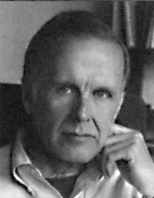
\includegraphics[height=1.9cm]{languages/pix/backus.jpg}% 
  \quad %\vspace*{1ex}
  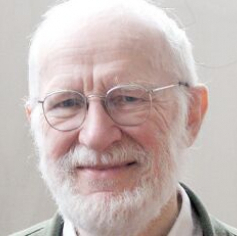
\includegraphics[height=1.9cm]{languages/pix/naur.jpg}}% 
  \wrapcaption{\label{fig:backus}\href{https://en.wikipedia.org/wiki/John_Backus}{John Backus 1924--2007}\index{Backus, J!picture} 与 \label{fig:naur}\href{https://en.wikipedia.org/wiki/Peter_Naur}{Peter Naur 1928--2016}\index{Naur, P!picture}}
\end{wrapfigure}


对文法（即短语结构和造句规则）的研究有着悠久的历史，最早可以追溯到公元前五世纪。
包括 A. Thue 和 E. Post 在内的数学家，在二十世纪初开始将其系统化为重写规则。
这里介绍的这个变体是在 20 世纪 50 年代末，由 J. Backus（约翰·巴科斯）创制，P. Naur（彼得·诺尔）亦有贡献，作为早期计算机语言 ALGOL60 设计工作的一部分。
自那时起，这些规则已成为
\citetext{描述文法的最常用方式}{%
  影响其被采用的一个因素，是 D. Knuth 写给《ACM 通讯》的一封信 \autocite{KnuthCACM}。
  他列举了 BNF 相对于当时广泛使用的文法描述方法的一些优点。
  最重要的是，他对比了 BNF 使用诸如 `\texttt{<addition operator>}` 这样的描述性文本来表示句法范畴，而不是像 `\texttt{A}` 这样的符号，
  并指出这一差异极大地增强了“语法的\textit{解释力}”。
  他还提议了“Backus Naur Form”这个名字。
  （现在最常见的是带有连字符的形式。）
}.\footnote{%
  BNF 的定义较为宽泛。
  虽然有标准，但资料往往并不完全符合任何单一标准。}

% \margingraphic[r]{0.15\textwidth}{languages/pix/naur.jpg}{\label{fig:naur}\href{https://en.wikipedia.org/wiki/Peter_Naur}{Peter Naur 1928--2016}}\index{Naur, P!picture}
与\zcref{sec:Grammars}的一个区别在于排版。
包括 `$\rightarrow$' 在内的元字符，在当时的标准键盘上无法输入。
% The advantage of having metacharacters not on a keyboard is that
% most likely all of the language characters are typeable
% so there is no need to distinguish, say, between the pipe character $\str{|}$
% when used as a part of a language and when used as a metacharacter.
% But the disadvantage lies in having to type the untypeable.
% In the end the convenience of having typeable characters 
% won over the technical gain of having to typographically distinguish 
% metacharacters.\index{metacharacter}
% For instance, for a long time standard keyboards had no arrows
BNF 取而代之使用了 `\bnfsymbol'。\footnote{%
  另一个排版问题是，虽然许多作者和我们一样使用尖括号加斜体来书写非终结符，但也有些作者仅仅依赖不同的字体样式或颜色，或者干脆用大写字母来表示非终结符。}
% (These adjustments were made by P~Naur as editor of the ALGOL60 
% report.)

\begin{example}
下面这个用于具有有限小数部分的实数的 Backus–Naur 范式（BNF）文法扩展了\zcref{ex:grammarForNaturals}。
\begin{grammar}
\ntrm{finite-real} \bnfproduces{}  \trm{-}\ntrm{fraction}
        \syntaxor \trm{+}\ntrm{fraction} 
        \syntaxor \ntrm{fraction}                

\ntrm{fraction} 
     \bnfproduces{} \ntrm{natural} 
       \syntaxor \ntrm{natural}\trm{.}\ntrm{natural}     

\ntrm{natural} 
     \bnfproduces{} \ntrm{digit} 
       \syntaxor \ntrm{digit}\ntrm{natural}     

\ntrm{digit} 
     \bnfproduces{} \trm{0} \syntaxor $\ldots$ \trm{9}     
\end{grammar}
\str{2.718} 的如下推导是最右推导。
\begin{displayedsteps}
  \initialstep\ntrm{finite-real}
  \derives\ntrm{fraction}
  \derives\ntrm{natural}\trm{.}\ntrm{natural}            
  \derives\ntrm{natural}\trm{.}\ntrm{digit}\ntrm{natural}
  \derives\ntrm{natural}\trm{.}\ntrm{digit}\ntrm{digit}\ntrm{natural}  
  \derives\ntrm{natural}\trm{.}\ntrm{digit}\ntrm{digit}\ntrm{digit}
  \derives\ntrm{natural}\trm{.}\ntrm{digit}\ntrm{digit}\trm{8}  
  \derives\ntrm{natural}\trm{.}\ntrm{digit}\trm{18}
  \derives\ntrm{natural}\trm{.718} 
  \derives\trm{2.718}
\end{displayedsteps}
下面是 \trm{0.577} 的一个推导，它既不是最左推导，也不是最右推导。
\begin{displayedsteps}
  \initialstep\ntrm{finite-real}
  \derives\ntrm{fraction}
  \derives\ntrm{natural}\trm{.}\ntrm{natural}            
  \derives\ntrm{natural}\trm{.}\ntrm{digit}\ntrm{natural}
  \derives\ntrm{natural}\trm{.5}\ntrm{natural}  
  \derives\ntrm{natural}\trm{.5}\ntrm{digit}\ntrm{natural}
  \derives\ntrm{digit}\trm{.5}\ntrm{digit}\ntrm{natural} 
  \derives\ntrm{digit}\trm{.5}\ntrm{digit}\ntrm{digit}  
  \derives\ntrm{digit}\trm{.5}\ntrm{digit}\trm{7}
  \derives\trm{0.5}\ntrm{digit}\trm{7} 
  \derives\trm{0.577}
\end{displayedsteps}
\end{example}

\begin{example}
\citetext{时间是一个棘手的工程问题}{% 
  %see https://zachholman.com/talk/utc-is-enough-for-everyone-right
  时间的复杂性有很多方面，其中之一便是闰秒。
  地球因潮汐的制动作用而不断减速。
  地球的平均减速幅度大约为每个世纪每天减慢 $1.4$ 毫秒，尽管具体数值因年而异，取决于包括大地震和火山喷发在内的许多因素。
  为确保原子钟时间与地球自转时间相差不超过 $0.9$ 秒，民用时间偶尔会增加额外的一秒。
  这个闰秒可以是正的也可以是负的，具体取决于地球的自转\Dash 有时会出现仅有 $58$ 秒的分钟，有时则会出现 $60$ 秒的分钟。

  更添混乱的是，自转变化并不均匀，我们无法预测遥远的未来的闰秒。
  国际地球自转服务会发布公告，提前几周通知将要增加的闰秒。
  因此，没有办法确定当前时刻到（例如）十年后之间一共会有多少秒。
  （这会引发诸如导航和高频交易等领域的麻烦，因此有提议要取消闰秒或用闰小时替代。）
  自1972年首次引入闰秒以来，所有的闰秒都是正的，在截至2006年1月的34年间共增加了23个闰秒。
  \autocite{web:USNO}}。
其中一个问题是时间的表示，该领域的一个标准是 \citetext{RFC~3339}{\autocite{rfc3339}}，即《互联网上的日期与时间：时间戳》。
它使用 \citetext{诸如 \str{1958-10-12T23:20:50.52Z} 这样的串}{%
  这种格式有许多优点，包括人类可读性好、对这些串进行排序时较早的时间排在前面、格式简单（只有一种格式），以及包含时区信息。}。
以下是 \citetext{其 BNF 文法}{%
  几点说明：
  (1)~协调世界时是民用时间的基础，常被称为 UTC，但有时也缩写为 Z，读作“Zulu”；
  (2)~年份用四位数字以防止 Y2K 问题 \autocite{y2k}；
  (3)~允许的月份数字仅为 $01$--$12$，且每个月中只允许特定的日期数字；
  (4)~允许的小时仅为 $00$--$23$，分钟必须在 $00$--$59$ 的范围内，等等。 \autocite{rfc3339}} 的部分内容。
%(See \zcref{exer:GrammarsForSmallLangs} for some nonterminals.)
（它包含了下文将讨论的元字符扩展。）

% % https://www.ietf.org/rfc/rfc3339.txt
   % date-month      = 2DIGIT  ; 01-12
   % date-mday       = 2DIGIT  ; 01-28, 01-29, 01-30, 01-31 based on
   %                           ; month/year
   % time-hour       = 2DIGIT  ; 00-23
   % time-minute     = 2DIGIT  ; 00-59
   % time-second     = 2DIGIT  ; 00-58, 00-59, 00-60 based on leap second
   %                           ; rules
   % time-secfrac    = "." 1*DIGIT
   % time-numoffset  = ("+" / "-") time-hour ":" time-minute
   % time-offset     = "Z" / time-numoffset

   % partial-time    = time-hour ":" time-minute ":" time-second
   %                   [time-secfrac]
   % full-date       = date-fullyear "-" date-month "-" date-mday
   % full-time       = partial-time time-offset

   % date-time       = full-date "T" full-time
\begin{grammar}
\ntrm{date-fullyear} \bnfproduces{} \ntrm{4-digits}

\ntrm{date-month} \bnfproduces{} \ntrm{2-digits}

\ntrm{date-mday} \bnfproduces{} \ntrm{2-digits} 

\ntrm{time-hour} \bnfproduces{} \ntrm{2-digits}

\ntrm{time-minute} \bnfproduces{} \ntrm{2-digits}  

\ntrm{time-second} \bnfproduces{} \ntrm{2-digits} 

\ntrm{time-secfrac} \bnfproduces{} \trm{.} \ntrm{1-or-more-digits}

\ntrm{time-numoffset} \bnfproduces{} (\trm{+}\syntaxor\trm{-}) \ntrm{time-hour} \trm{:} \ntrm{time-minute}

\ntrm{time-offset} \bnfproduces{} \trm{Z} \syntaxor \ntrm{time-numoffset}

\ntrm{partial-time} \bnfproduces{} \ntrm{time-hour} \trm{:} \ntrm{time-minute} \trm{:} \ntrm{time-second} [\ntrm{time-secfrac}]

\ntrm{full-date} \bnfproduces{} \ntrm{date-fullyear} \trm{-} \ntrm{date-month} \trm{-} \ntrm{date-mday}

\ntrm{full-time} \bnfproduces{} \ntrm{partial-time} \ntrm{time-offset}

\ntrm{date-time} \bnfproduces{} \ntrm{full-date} \trm{T} \ntrm{full-time}
\end{grammar}
\end{example}

有许多扩展的 Backus–Naur 范式记法，它们已不仅仅是简单的字符替换。
上面的 `\ntrm{partial-time}` 规则展示了其中一种，它使用方括号作为元字符，表示 `\ntrm{time-secfrac}` 是可选的。
这是一种非常常见的结构：另一个例子是下面带有可选 `\str{else}` 的 `\str{if $\ldots$ then $\ldots$}` 语法描述。

\begin{grammar}
    \ntrm{if-stmt} \bnfproduces{}  \trm{if} \ntrm{boolean-expr} \trm{then}
                             \ntrm{stmt-sequence}\\*
                        \quad[ \trm{else}
                             \ntrm{stmt-sequence} ]
                        \ntrm{end-if} \trm{;}
\end{grammar}

为了表示“零次或多次”的重复，BNF 使用 Kleene 星，~$\kleenestar{}$\!。

\begin{grammar}
 \ntrm{string} \bnfproduces{} \ntrm{letter}\trm{*}
\end{grammar}

为了表达“一次或多次”，BNF 使用加号~\trm{+}。

\begin{example} \label{ex:PythonFloatingPoint}
这个关于 Python 浮点数的文法同时展示了方括号和加号。

\begin{grammar}
\ntrm{floatnumber}   \bnfproduces{}  \ntrm{pointfloat} \syntaxor \ntrm{exponentfloat}

\ntrm{pointfloat}    \bnfproduces{}  [\ntrm{intpart}] \ntrm{fraction} \syntaxor \ntrm{intpart} \trm{.}

\ntrm{exponentfloat} \bnfproduces{}  (\ntrm{intpart} \syntaxor \ntrm{pointfloat}) \ntrm{exponent}

\ntrm{intpart}       \bnfproduces{}  \ntrm{digit}+

\ntrm{fraction}      \bnfproduces{}  \trm{.} \ntrm{digit}+

\ntrm{exponent}      \bnfproduces{}  (\trm{e}\syntaxor{}\trm{E}) [\trm{+}\syntaxor{}\trm{-}] \ntrm{digit}+
\end{grammar}

\noindent 在 \ntrm{pointfloat} 规则中，第一个 \ntrm{intpart} 是可选的。
而一个 \ntrm{intpart} 由一个或多个数字组成。
\end{example}

这些扩展并非必需，因为即使没有它们，我们也能表达这些文法。
例如，我们可以将下面这个使用 Kleene 星的文法

\begin{grammar}
 \ntrm{string} \bnfproduces{} \ntrm{letter}\trm{*}
\end{grammar}

\noindent 替换为如下文法。

\begin{grammar}
\ntrm{string} \bnfproduces{} \ntrm{letter}\ntrm{string} \syntaxor \emptystring 
\end{grammar}

\noindent 但这些构造出现的频率足够高，采用缩写形式会带来极大的便利。

从文法到其语法分析器的转换是机械性的过程。
有些程序将文法（通常是 BNF 形式的）作为输入，并输出能够对符合该文法格式的文件进行语法分析的源代码。
这种程序称为 \definend{语法分析器生成器（parser-generator）}\index{parser-generator} 
（有时也被称为
\definend{编译器的编译器（compiler-compiler）},\index{compiler-compiler}
这个词很有趣，但有误导性，因为语法分析器只是编译器的一部分）。

\medskip
总而言之，
BNF 能够表达我们通常想要表达的语言范围（上下文无关文法），
并且能够平滑地转化为语法分析器。
它的优点是简洁，同时在需要保持清晰的地方又不牺牲清晰性。
也就是说，BNF 是一种“阻抗匹配”\Dash 它契合我们的需求。

\begin{exercises}
\recommended


\begin{exercise}
美国的 ZIP 编码有五位数字，末尾可能还有一个短横线和额外的四位数字。
给出一个 BNF 文法。
\begin{answer}\verified
\begin{grammar}
\ntrm{zip} \bnfproduces{} \ntrm{digit}\ntrm{digit}\ntrm{digit}\ntrm{digit}\ntrm{digit}[-\ntrm{digit}\ntrm{digit}\ntrm{digit}\ntrm{digit}]

\ntrm{digit} \bnfproduces{} \trm{0} \syntaxor $\ldots${} \syntaxor \trm{9}    
\end{grammar}
\end{answer}
\end{exercise}

\begin{exercise}
使用 $\Sigma=\set{\str{a},\ldots\,\str{z}}$ 写一个回文语言的 BNF 文法。
\begin{answer}\verified
当我们在前面添加一个字符时，也同时在后面添加它。
\begin{grammar}
\ntrm{palindrome} \bnfproduces{} \trm{a} \ntrm{palindrome} \trm{a} 
    \syntaxor \trm{b} \ntrm{palindrome} \trm{b} 
    \syntaxor $\ldots${}
       \trm{z} \ntrm{palindrome} \trm{z} 
   \syntaxor \ntrm{letter} \syntaxor \emptystring

\ntrm{letter} \bnfproduces{} \trm{a} \syntaxor $\ldots${} 
  \trm{z}    
\end{grammar}
注意，这里将 \emptystring{} 也视作回文。
\end{answer}
\end{exercise}

\recommended


\begin{exercise}
在某大学，课程代码的格式类似于 `MA~208' 或 `PSY~101'，其中院系代码是两到三个大写字母，课程号是三位数字。
给出一个 BNF 文法。
\begin{answer}\verified
这是一种写法。
\begin{grammar}
\ntrm{course code} \bnfproduces{} \ntrm{dept} \ntrm{space} \ntrm{course-number}

\ntrm{dept} \bnfproduces{} \ntrm{two-letter} \syntaxor \ntrm{three-letter} 

\ntrm{two-letter} \bnfproduces{} \ntrm{letter}\ntrm{letter}

\ntrm{three-letter} \bnfproduces{} \ntrm{two-letter}\ntrm{letter}

\ntrm{course-number} \bnfproduces{} \ntrm{digit}\ntrm{digit}\ntrm{digit}

\ntrm{digit} \bnfproduces{} \trm{0} \syntaxor $\ldots${} \trm{9}       

\ntrm{letter} \bnfproduces{} \trm{A} \syntaxor $\ldots${} \trm{Z}       
\end{grammar}
非终结符 \ntrm{space} 生成一个难以直观显示的空格。

我们也可以像下面这样，逐个列举院系名称。
\begin{grammar}
\ntrm{dept} \bnfproduces{} \trm{MA} \syntaxor \trm{PSY} \syntaxor $\ldots${}
\end{grammar}
这种做法更符合实际，不会允许无意义的院系名称。
但其维护上的劣势在于，如果院系代码发生变化，文法描述也必须随之修改。
（在文法中强制要求符合实际往往要付出代价。）
\end{answer}
\end{exercise}

\recommended

\begin{exercise}
\zcref{ex:PythonFloatingPoint}使用了一些 BNF 便利缩写。
\begin{exparts*}
\item
给出与 \ntrm{pointfloat} 等价，但不使用方括号的规则。
\item
类似地，替换 \ntrm{intpart} 规则中的重复算子，以及 \ntrm{exponent} 规则中的方括号和重复算子。
\end{exparts*}
\begin{answer}\verified
\begin{exparts}
\item
可以这样改写。

\begin{grammar}
\ntrm{pointfloat} \bnfproduces{} \ntrm{intpart} \ntrm{fraction} 
    \syntaxor \ntrm{fraction} 
    \syntaxor \ntrm{intpart} \trm{.}
\end{grammar}
\item
用递归来替换 $+$ 算子。
\begin{grammar}
\ntrm{intpart} \bnfproduces{} \ntrm{intpart} \ntrm{digit} 
    \syntaxor \ntrm{digit} 
\end{grammar}
对于 \ntrm{exponent}，列举各种情况。
\begin{grammar}
\ntrm{exponent} \bnfproduces{}
    \trm{e} \ntrm{intpart}  
    \syntaxor \trm{e+} \ntrm{intpart} 
    \syntaxor \trm{e-} \ntrm{intpart} 
    \syntaxor \trm{E} \ntrm{intpart} 
    \syntaxor \trm{E+} \ntrm{intpart} 
    \syntaxor \trm{E-} \ntrm{intpart} 
\end{grammar} 
\end{exparts}
\end{answer}
\end{exercise}

\recommended


\begin{exercise}
在罗马数字中，
字母 I, V, X, L, C, D 和 M 分别代表数值
$1$、$5$、$10$、$50$、$100$、$500$ 和 $1000$。
我们用这些字母从左到右按数值降序排列来表示自然数，
因此 XVI 代表的数在十进制记法中是 $16$，
而 M{}D{}C{}C{}C{}C{}L{}V{}I{}I{}I 代表 $1958$。
我们总是写尽可能短的字符串，
因此我们不会写 I{}I{}I{}I{}I，因为可以改写为 V。
然而，由于我们没有值大于 $1000$ 的符号，
所以必须用很多 M 来表示大数。
\begin{exparts}
\item
给出一个能生成合理的罗马数字串的文法。
\item
罗马数字也常以减法记法书写：例如，$4$ 表示为 I{}V，
因为在表盘等场合，四个 I 与三个 I 很难区分。
在这种记法中，$9$ 是 I{}X，
$40$ 是 X{}L，
$90$ 是 X{}C，
$400$ 是 C{}D，
$900$ 是 C{}M。
给出一个扩展的 BNF 文法，用于生成这种记法中可能出现的字符串。
\end{exparts}
\begin{answer}\verified
\begin{exparts}
\item
这是标准表示法的文法。
\begin{grammar}
\ntrm{roman-numeral} \bnfproduces{} \ntrm{thousands} \ntrm{hundreds} \ntrm{tens} \ntrm{ones}

\ntrm{thousands} \bnfproduces{} \trm{M}\trm{*}     

\ntrm{hundreds} \bnfproduces{} \trm{C} \syntaxor \trm{CC} \syntaxor \trm{CCC} 
   \syntaxor \trm{CCCC}  \syntaxor \trm{D}  \syntaxor \trm{DC}  
   \syntaxor \trm{DCC}  \syntaxor \trm{DCCC}  \syntaxor \trm{DCCCC} 
   \syntaxor \emptystring{}

\ntrm{tens} \bnfproduces{} \trm{X} \syntaxor \trm{XX} \syntaxor \trm{XXX}
    \syntaxor \trm{XXXX}  \syntaxor \trm{L} \syntaxor \trm{LX}
    \syntaxor \trm{LXX}  \syntaxor \trm{LXXX}  \syntaxor \trm{LXXXX}
    \syntaxor \emptystring{}

\ntrm{ones} \bnfproduces{} \trm{I} \syntaxor \trm{II} \syntaxor \trm{III}
     \syntaxor \trm{IIII}  \syntaxor \trm{V}  \syntaxor \trm{VI}  \syntaxor \trm{VII}
      \syntaxor \trm{VIII}  \syntaxor \trm{VIIII}  \syntaxor \emptystring{} 
\end{grammar}
\item
这是减法记法的罗马数字文法。

\begin{grammar}
\ntrm{roman-numeral} \bnfproduces{} \ntrm{thousands} \ntrm{hundreds} \ntrm{tens} \ntrm{ones}

\ntrm{thousands} \bnfproduces{} \trm{M}\trm{*}     

\ntrm{hundreds} \bnfproduces{} \trm{CM} \syntaxor \trm{CD} \syntaxor (\trm{D} \syntaxor \emptystring) (\emptystring \syntaxor \trm{C} \syntaxor \trm{CC} \syntaxor \trm{CCC} )   

\ntrm{tens} \bnfproduces{} \trm{XC} \syntaxor \trm{XL} \syntaxor ( \trm{L}| \emptystring ) ( \emptystring\syntaxor \trm{X} \syntaxor \trm{XX} \syntaxor \trm{XXX})  

\ntrm{ones} \bnfproduces{} \trm{IX} \syntaxor \trm{IV} \syntaxor ( \trm{V} 
  \syntaxor \emptystring ) ( \emptystring \syntaxor \trm{I} \syntaxor \trm{II} \syntaxor \trm{III} )            
\end{grammar}
\end{exparts}
\end{answer}
\end{exercise}

\begin{exercise}
\begin{credit}
  \url{http://people.cs.ksu.edu/~schmidt/300s05/Lectures/GrammarNotes/bnf.html}
\end{credit}
下面的文法描述了一种类 C 的小型编程语言。
\begin{grammar}
\ntrm{program} \bnfproduces{} \trm{\{} \ntrm{statement-list} \trm{\}}

\ntrm{statement-list} \bnfproduces{} [ \ntrm{statement} \trm{;} ]\trm{*}

\ntrm{statement} \bnfproduces{} \ntrm{data-type} \ntrm{identifier}
               \othersyntax \ntrm{identifier} \trm{=} \ntrm{expression}
	       \othersyntax \trm{print} \ntrm{identifier}
	       \othersyntax \trm{while} \ntrm{expression} \trm{\{} \ntrm{statement-list} \trm{\}}

\ntrm{data-type} \bnfproduces{} \trm{int} \syntaxor \trm{boolean}

\ntrm{expression} \bnfproduces{} \ntrm{identifier} \syntaxor \ntrm{number} \syntaxor \trm{(} \ntrm{expression} \ntrm{operator} \ntrm{expression} \trm{)}

\ntrm{identifier} \bnfproduces{}  \ntrm{letter} [ \ntrm{letter} ]\trm{*}

\ntrm{number} \bnfproduces{}  \ntrm{digit} [ \ntrm{digit} ]\trm{*}

\ntrm{operator} \bnfproduces{} \trm{+} \syntaxor \trm{==}

\ntrm{letter} \bnfproduces{} \trm{A} \syntaxor $\ldots${} \syntaxor \trm{Z}

\ntrm{digit} \bnfproduces{} \trm{0} \syntaxor $\ldots${} \syntaxor \trm{9}    
\end{grammar}
\begin{exparts}
\item 为下面的程序给出一个推导和语法分析树。
\begin{lstlisting}
{ int A ;
  A = 1 ;  
  print A ;
}
\end{lstlisting}
% \item Give a parse tree for this program.
% \begin{lstlisting}
% { int A ;
%   A = 5 ;
%   while  ( A == 5 )  { int B ; B = 6 ;  A = ( B + A ) ;
%                        print A ; } ;
%   boolean C ;  print C ;
% }
% \end{lstlisting}
\item 所有程序都必须被花括号包围吗？  
\end{exparts}
\begin{answer}\verified
  \begin{exparts}
  \item 下面是一个推导。为了简洁起见，我们做了缩写，例如在第三行一次性放入了多个
    \ntrm{statement}，而不是逐个放入。
  \begin{displayedsteps}
    \initialstep\ntrm{program}
    \derives\trm{\{} \ntrm{statement-list} \trm{\}}
    \\
    \derives\trm{\{} \ntrm{statement} \trm{;} \ntrm{statement} \trm{;} \ntrm{statement} \trm{;} \trm{\}}
    \\
    \derives\trm{\{} \ntrm{data-type} \ntrm{identifier} \trm{;} \ntrm{statement} \trm{;} \ntrm{statement} \trm{;} \trm{\}}
    \\
    \derives\trm{\{} \trm{int} \ntrm{identifier} \trm{;} \ntrm{statement} \trm{;} \ntrm{statement} \trm{;} \trm{\}}
    \\
    \derives\trm{\{} \trm{int} \ntrm{letter} \trm{;} \ntrm{statement} \trm{;} \ntrm{statement} \trm{;} \trm{\}}
    \\
    \derives\trm{\{} \trm{int} \trm{A} \trm{;} \ntrm{statement} \trm{;} \ntrm{statement} \trm{;} \trm{\}}
    \\
    \derives\trm{\{} \trm{int} \trm{A} \trm{;} \ntrm{identifier} \trm{=} \ntrm{expression} \trm{;} \ntrm{statement} \trm{;} \trm{\}}
    \\
    \derives\trm{\{} \trm{int} \trm{A} \trm{;} \ntrm{letter} \trm{=} \ntrm{expression} \trm{;} \ntrm{statement} \trm{;} \trm{\}}
    \\
    \derives\trm{\{} \trm{int} \trm{A} \trm{;} \trm{A} \trm{=} \ntrm{expression} \trm{;} \ntrm{statement} \trm{;} \trm{\}}
    \\
    \derives\trm{\{} \trm{int} \trm{A} \trm{;} \trm{A} \trm{=} \ntrm{number} \trm{;} \ntrm{statement} \trm{;} \trm{\}}
    \\
    \derives\trm{\{} \trm{int} \trm{A} \trm{;} \trm{A} \trm{=} \ntrm{digit} \trm{;} \ntrm{statement} \trm{;} \trm{\}}
    \\
    \derives\trm{\{} \trm{int} \trm{A} \trm{;} \trm{A} \trm{=} \trm{1} \trm{;} \ntrm{statement} \trm{;} \trm{\}}
    \\
    \derives\trm{\{} \trm{int} \trm{A} \trm{;} \trm{A} \trm{=} \trm{1} \trm{;} \trm{print} \ntrm{identifier} \trm{;} \trm{\}}
    \\
    \derives\trm{\{} \trm{int} \trm{A} \trm{;} \trm{A} \trm{=} \trm{1} \trm{;} \trm{print} \ntrm{letter} \trm{;} \trm{\}}
    \\
    \derives\trm{\{} \trm{int} \trm{A} \trm{;} \trm{A} \trm{=} \trm{1} \trm{;} \trm{print} \trm{A} \trm{;} \trm{\}}
  \end{displayedsteps}
  语法分析树见\figureref{fig:CLikeLang}。
  \begin{figure}
    \centering
    \includegraphics{languages/asy/parsetree/parsetree1000.pdf}
    \caption{类 C 语言的语法分析树}
    \label{fig:CLikeLang}
  \end{figure}
  \item 是的，因为所有推导都必须从 \ntrm{program} 出发并经过
    \ntrm{statement-list}，这迫使它们带有花括号。
  \end{exparts}
\end{answer}
\end{exercise}

\begin{exercise}
下面是一个 LISP 的文法。
\begin{grammar}
\ntrm{s-expression} \bnfproduces{} \ntrm{atomic-symbol}
                   \othersyntax\trm{(} \ntrm{s-expression} \trm{.} \ntrm{s-expression} \trm{)}
                   \othersyntax \ntrm{list}

\ntrm{list} \bnfproduces{} \trm{(} \ntrm{s-expression}\trm{*} \trm{)}

\ntrm{atomic-symbol} \bnfproduces{} \ntrm{letter} \ntrm{atom-part}

\ntrm{atom-part} \bnfproduces{} \ntrm{empty}
                \othersyntax \ntrm{letter} \ntrm{atom-part}
                \othersyntax \ntrm{number} \ntrm{atom-part}

\ntrm{letter} \bnfproduces{} \trm{a} \syntaxor \trm{b} \syntaxor $\ldots${}  \trm{z}

\ntrm{number} \bnfproduces{} \trm{1} \syntaxor \trm{2} \syntaxor $\ldots${}  \trm{9}   
\end{grammar}
此外还有一条规则：\ntrm{empty} 产生一个空格 
\mbox{\trm{" "}}。
推导 s-表达式 \str{(cons (car x) y)}。
\begin{answer}\verified
  在下面的部分推导中，我们做了一些缩写，例如一次性放入多个 \ntrm{s-expression} 来形成
  \ntrm{list}，而不是每次只放一个。
  \begin{displayedsteps}
    \initialstep\ntrm{s-expression}
    \derives \ntrm{list}
    \\
    \derives\trm{(} \ntrm{s-expression} \ntrm{s-expression} \ntrm{s-expression} \trm{)}
    \\
    \derives\trm{(} \ntrm{s-expression} \ntrm{list} \ntrm{s-expression} \trm{)}
    \\
    \derives\trm{(} \ntrm{s-expression} \trm{(} \ntrm{s-expression} \ntrm{s-expression} \trm{)} \ntrm{s-expression} \trm{)}
    \\
    \derives\trm{(} \ntrm{atomic-symbol} \trm{(} \ntrm{s-expression} \ntrm{s-expression} \trm{)} \ntrm{s-expression} \trm{)}
    \\
    \derives\trm{(} \ntrm{letter} \ntrm{atom-part} \trm{(} \ntrm{s-expression} \ntrm{s-expression} \trm{)} \ntrm{s-expression} \trm{)}
    \\
    \derives\trm{(} \ntrm{letter} \ntrm{letter} \ntrm{atom-part} \trm{(} \ntrm{s-expression} \ntrm{s-expression} \trm{)} \ntrm{s-expression} \trm{)}
    \\
    \derives\trm{(} \ntrm{letter} \ntrm{letter} \ntrm{letter} \ntrm{atom-part} \trm{(} \ntrm{s-expression} \ntrm{s-expression} \trm{)} \ntrm{s-expression} \trm{)}
    \\
    \derives\trm{(} \ntrm{letter} \ntrm{letter} \ntrm{letter} \ntrm{letter} \ntrm{atom-part} \trm{(} \ntrm{s-expression} \ntrm{s-expression} \trm{)} \ntrm{s-expression} \trm{)}
    \\
    \derives\trm{(} \ntrm{letter} \ntrm{letter} \ntrm{letter} \ntrm{letter}  \ntrm{atom-part}  \trm{(} \ntrm{s-expression} \ntrm{s-expression} \trm{)} \ntrm{s-expression} \trm{)}
    \\
    \derives\trm{(} \trm{c} \ntrm{letter} \ntrm{letter} \ntrm{letter}  \ntrm{atom-part} \trm{(} \ntrm{s-expression} \ntrm{s-expression} \trm{)} \ntrm{s-expression} \trm{)}
    \\
    \derives\trm{(} \trm{c} \trm{o} \ntrm{letter} \ntrm{letter}  \ntrm{atom-part}  \trm{(} \ntrm{s-expression} \ntrm{s-expression} \trm{)} \ntrm{s-expression} \trm{)}
    \\
    \derives\trm{(} \trm{c} \trm{o} \trm{n} \ntrm{letter}  \ntrm{atom-part}  \trm{(} \ntrm{s-expression} \ntrm{s-expression} \trm{)} \ntrm{s-expression} \trm{)}
    \\
    \derives\trm{(} \trm{c} \trm{o} \trm{n} \trm{s}  \ntrm{atom-part} \trm{(} \ntrm{s-expression} \ntrm{s-expression} \trm{)} \ntrm{s-expression} \trm{)}
    \\
    \derives\trm{(} \trm{c} \trm{o} \trm{n} \trm{s}  \ntrm{empty} \trm{(} \ntrm{s-expression} \ntrm{s-expression} \trm{)} \ntrm{s-expression} \trm{)}
    \\
    \derives\trm{(} \trm{c} \trm{o} \trm{n} \trm{s}  \trm{" "} \trm{(} \ntrm{s-expression} \ntrm{s-expression} \trm{)} \ntrm{s-expression} \trm{)}
  \end{displayedsteps}
  将剩余的非终结符展开为字母很繁琐，因此我们到此为止。
\end{answer}
\end{exercise}

\begin{exercise}
Python 3的格式规范迷你语言（Format Specification Mini-Language）用于描述字符串替换。
\begin{grammar}
  \ntrm{format-spec} \bnfproduces{}  [[\ntrm{fill}]\ntrm{align}][\ntrm{sign}][\trm{\#}][\trm{0}][\ntrm{width}][\ntrm{gr}][\trm{.}\ntrm{precision}][\ntrm{type}]

\ntrm{fill}            \bnfproduces{}  \ntrm{any character}

\ntrm{align}           \bnfproduces{}  \trm{<} \syntaxor \trm{>} \syntaxor \trm{=} \syntaxor \trm{\^{}}

\ntrm{sign}            \bnfproduces{}  \trm{+} \syntaxor \trm{-} \syntaxor \trm{ }

\ntrm{width}           \bnfproduces{}  \ntrm{integer}

\ntrm{gr} \bnfproduces{}  \trm{-} \syntaxor \trm{,}

\ntrm{precision}       \bnfproduces{}  \ntrm{integer}

\ntrm{type}            \bnfproduces{}  \trm{b} \syntaxor \trm{c} \syntaxor \trm{d} \syntaxor \trm{e} \syntaxor \trm{E} \syntaxor \trm{f} \syntaxor \trm{F} \syntaxor \trm{g} \syntaxor \trm{G} \syntaxor \trm{n} \syntaxor \trm{o} \syntaxor \trm{s} \syntaxor \trm{x} \syntaxor \trm{X} \syntaxor \trm{\%}  
\end{grammar}
规定 \ntrm{integer} 可生成
\mbox{\ntrm{digit} \ntrm{integer}}
或 \ntrm{digit}。
为以下字符串给出推导过程：
\begin{exparts*}
\item \str{03f}
\item \str{+\#02X}.
\end{exparts*}
\begin{answer}\verified
\begin{exparts}
\item
  例如，这里我们将利用 BNF 记法一次替换多个非终结符，而不是每次只替换一个。
  \begin{displayedsteps}
    \initialstep\ntrm{format-spec}
    \derives \trm{0} \ntrm{width} \ntrm{type}
    \\
    \derives \trm{0} \ntrm{integer} \ntrm{type}
    \\
    \derives \trm{0} \ntrm{digit} \ntrm{type}
    \\
    \derives \trm{0} \trm{3} \ntrm{type}
    \\
    \derives \trm{0} \trm{3} \trm{f}
  \end{displayedsteps}
\item
  \begin{displayedsteps}
    \initialstep\ntrm{format-spec}
    \derives \ntrm{sign} \trm{\#} \trm{0} \ntrm{width} \ntrm{type}
    \\
    \derives \trm{+} \trm{\#} \trm{0} \ntrm{width} \ntrm{type}
    \\
    \derives \trm{+} \trm{\#} \trm{0} \ntrm{integer} \ntrm{type}
    \\
    \derives \trm{+} \trm{\#} \trm{0} \ntrm{digit} \ntrm{type}
    \\
    \derives \trm{+} \trm{\#} \trm{0} \trm{2} \ntrm{type}
    \\
    \derives \trm{+} \trm{\#} \trm{0} \trm{2} \trm{X}
  \end{displayedsteps}
\end{exparts}
\end{answer}
\end{exercise}

% \begin{exercise}
% This is the grammar of BNF, written in BNF.
% \begin{grammar}
% \ntrm{syntax}         \bnfproduces{} \ntrm{rule} \syntaxor \ntrm{rule} \ntrm{syntax}

%  \ntrm{rule}           \bnfproduces{} \ntrm{opt-whitespace} \trm{<} \ntrm{rule-name} \trm{>} \ntrm{opt-whitespace} \trm{::=} \ntrm{opt-whitespace} \ntrm{expression} \ntrm{line-end}

%  \ntrm{opt-whitespace} \bnfproduces{} \trm{" "} \ntrm{opt-whitespace} \syntaxor \emptystring{}

%  \ntrm{expression}     \bnfproduces{} \ntrm{list} \syntaxor \ntrm{list} \ntrm{opt-whitespace} \trm{|} \ntrm{opt-whitespace} \ntrm{expression}

%  \ntrm{line-end}       \bnfproduces{} \ntrm{opt-whitespace} \ntrm{EOL} \syntaxor \ntrm{line-end} \ntrm{line-end}

%  \ntrm{list}           \bnfproduces{} \ntrm{term} \syntaxor \ntrm{term} \ntrm{opt-ws} \ntrm{list}

%  \ntrm{term}           \bnfproduces{} \ntrm{literal} \syntaxor \trm{<} \ntrm{rule-name} \trm{>}

%  \ntrm{literal}        \bnfproduces{} \textdoublequote{} \ntrm{text1} \textdoublequote{} \syntaxor \textsinglequote{} \ntrm{text2} \textsinglequote{}

%  \ntrm{text1}          \bnfproduces{} \emptystring \syntaxor \ntrm{character1} \ntrm{text1}

%  \ntrm{text2}          \bnfproduces{} \emptystring \syntaxor \ntrm{character2} \ntrm{text2}

%  \ntrm{character}      \bnfproduces{} \ntrm{letter} \syntaxor \ntrm{digit} \syntaxor \ntrm{symbol}

%  \ntrm{letter}         \bnfproduces{} \trm{A} \syntaxor \trm{B} \syntaxor \ldots{} \trm{z} 

% % \trm{C} \syntaxor \trm{D} \syntaxor \trm{E} \syntaxor \trm{F} \syntaxor \trm{G} \syntaxor \trm{H} \syntaxor \trm{I} \syntaxor \trm{J} \syntaxor \trm{K} \syntaxor \trm{L} \syntaxor \trm{M} \syntaxor \trm{N} \syntaxor \trm{O} \syntaxor \trm{P} \syntaxor \trm{Q} \syntaxor \trm{R} \syntaxor \trm{S} \syntaxor \trm{T} \syntaxor \trm{U} \syntaxor \trm{V} \syntaxor \trm{W} \syntaxor \trm{X} \syntaxor \trm{Y} \syntaxor \trm{Z} \syntaxor \trm{a} \syntaxor \trm{b} \syntaxor \trm{c} \syntaxor \trm{d} \syntaxor \trm{e} \syntaxor \trm{f} \syntaxor \trm{g} \syntaxor \trm{h} \syntaxor \trm{i} \syntaxor \trm{j} \syntaxor \trm{k} \syntaxor \trm{l} \syntaxor \trm{m} \syntaxor \trm{n} \syntaxor \trm{o} \syntaxor \trm{p} \syntaxor \trm{q} \syntaxor \trm{r} \syntaxor \trm{s} \syntaxor \trm{t} \syntaxor \trm{u} \syntaxor \trm{v} \syntaxor \trm{w} \syntaxor \trm{x} \syntaxor \trm{y} \syntaxor \trm{z}

%  \ntrm{digit}          \bnfproduces{} \trm{0} \syntaxor \trm{1} \syntaxor 
%                        \ldots{} \trm{9}

% % \trm{2} \syntaxor \trm{3} \syntaxor \trm{4} \syntaxor \trm{5} \syntaxor \trm{6} \syntaxor \trm{7} \syntaxor \trm{8} \syntaxor \trm{9}

%  \ntrm{symbol}         \bnfproduces{}  \trm{|} \syntaxor \emptystring \syntaxor \trm{-} \syntaxor \trm{!} \syntaxor \trm{\#} \syntaxor \trm{\$} \syntaxor \trm{\%} \syntaxor \trm{\&} \syntaxor \trm{(} \syntaxor \trm{)} \syntaxor \trm{*} \syntaxor \trm{+} \syntaxor \trm{,} \syntaxor \trm{-} \syntaxor \trm{.} \syntaxor \trm{/} \syntaxor \trm{:} \syntaxor \trm{;} \syntaxor \trm{<} \syntaxor \trm{=} \syntaxor \trm{>} \syntaxor \trm{?} \syntaxor \trm{@} \syntaxor \trm{[} \syntaxor \trm{\textbackslash} \syntaxor \trm{]} \syntaxor \trm{\textasciicircum} \syntaxor \trm{-} \syntaxor \trm{`} \syntaxor \trm{{} \syntaxor \trm{\syntaxor} \syntaxor \trm{}} \syntaxor \trm{\textasciitilde}

%  \ntrm{character1}     \bnfproduces{} \ntrm{character} \syntaxor \trm{'}

%  \ntrm{character2}     \bnfproduces{} \ntrm{character} \syntaxor \textdoublequote

%  \ntrm{rule-name}      \bnfproduces{} \ntrm{letter} \syntaxor \ntrm{rule-name} \ntrm{rule-char}

%  \ntrm{rule-char}      \bnfproduces{} \ntrm{letter} \syntaxor \ntrm{digit} \syntaxor \trm{-}
% \end{grammar}
% \begin{exparts}
% \item Give a derivation of the rule \mbox{\ntrm{ab} \bnfproduces{} \ntrm{cd} e}.  
% \item Give a derivation of the rule \mbox{\ntrm{ab} \bnfproduces{} e \ntrm{cd}}.  
% \end{exparts}
% \end{exercise}
\end{exercises}
\index{BNF|)}

\extra{图遍历}\index{Graph traversal|(}\index{tree!traversal}\index{directed acyclic graph DAG!traversal} \label{extra:GraphTraversal}
在本书的多处，我们将描述如何遍历树或其他图。
例如，当我们描述枚举集合 $\N\times\N$ 的 Cantor 对应时，我们画了下面这个阵列。
\begin{equation*}
  \begin{array}{cccccc}
    \vdots          &\vdots         &\vdots         &\vdots         \\
    \sequence{0,3}  &\sequence{1,3} &\sequence{2,3} &\sequence{3,3} &\cdots  \\
    \sequence{0,2}  &\sequence{1,2} &\sequence{2,2} &\sequence{3,2} &\cdots  \\ 
    \sequence{0,1}  &\sequence{1,1} &\sequence{2,1} &\sequence{3,1} &\cdots  \\ 
    \sequence{0,0}  &\sequence{1,0} &\sequence{2,0} &\sequence{3,0} &\cdots
  \end{array}
\end{equation*}
我们可以将每个阵列元素与其上方的元素、以及与其右方的元素连接起来，从而构成一个图。
这里我们将左下角旋转到了顶部。


\begin{center}
  \vcenteredhbox{\includegraphics{languages/asy/graphs/graphs1031.pdf}}
\end{center}


这并不是一棵树，因为有些顶点之间存在不止一条路，例如
$\sequence{0,0}\to\sequence{0,1}\to\sequence{1,1}$
和
$\sequence{0,0}\to\sequence{1,0}\to\sequence{1,1}$。
相反，它是一个有向无环图。
% But it is like a tree in that there are no cycles.

Cantor 的枚举


\begin{center}
  \begin{tabular}{r|ccccccc@{\hspace{6pt}}c}
    \tabulartext{编号}
       &$0$    &$1$   &$2$  &$3$  &$4$  &$5$  &$6$ &\ldots
   \\ \cline{2-9}
    \tabulartext{数对}
               &$\sequence{0,0}$\rule{0pt}{10pt}
               &$\sequence{0,1}$
               &$\sequence{1,0}$
               &$\sequence{0,2}$
               &$\sequence{1,1}$
               &$\sequence{2,0}$
               &$\sequence{0,3}$
               &\ldots
     \end{tabular}
\end{center}


从上到下遍历此图。

我们将介绍两种遍历策略：
\definend{深度优先}\index{depth-first traversal}\index{graph!traversal!depth-first}
和
\definend{广度优先}。\index{breadth-first traversal}\index{graph!traversal!breadth-first}
下面的树展示了这两种策略。
表中第一行先访问一个节点的子节点，再去访问该节点的兄弟节点。
表中第二行先访问所有深度为 $k$ 的节点，再访问任何深度为 $k+1$ 的节点。（在一棵树中，一个节点的
\definend{深度}\index{graph!node!rank}\index{rank of a vertex}
是指从根节点到该节点的最短路中的边数。
在这个有向无环图中，它是指从源节点到该节点的最短路中的边数。）


\begin{center}
  \vcenteredhbox{\includegraphics{languages/asy/graphs/graphs1028.pdf}}
  \qquad
  \begin{tabular}{r|l}
    \multicolumn{1}{c}{\tabulartext{遍历方式}}
      &\multicolumn{1}{c}{\tabulartext{节点顺序}}  \\
    \hline 
    深度优先\rule{0pt}{11pt}
      &$a$-$b$-$e$-$f$-$c$-$d$-$g$-$i$-$j$-$h$ \\
    广度优先
      &$a$-$b$-$c$-$d$-$e$-$f$-$g$-$h$-$i$-$j$ \\
  \end{tabular}
  % \vcenteredhbox{\includegraphics{languages/asy/graphs/graphs1030.pdf}}
  % \qquad
  % \vcenteredhbox{\includegraphics{languages/asy/graphs/graphs1029.pdf}}
\end{center}

这里我们将编写 Racket 代码来遍历树和有向无环图。
代码首先定义一个 \codeinline{node}，本质上是一个有序对。
\lstinputlisting[firstline=15,lastline=15]{\traversefile}
Racket 的 \codeinline{struct} 构造会自动定义许多有用的函数。
其中一个是创建函数 \codeinline{(node n s)}，它用于创建节点。
它还创建了访问器函数 \codeinline{node-name} 和 \codeinline{node-children}，我们将在下面看到。

我们使用该创建函数来定义下一个函数。
\lstinputlisting[firstline=21,lastline=22]{\traversefile}
注意 \codeinline{children} 被创建为一个集合，以便我们可以快速访问其成员。
将这个集合设为可变的，意味着在创建树的过程中，我们可以向该集合中添加子节点来修改它。

我们使用那个例程来创建新树和单源有向无环图。
\lstinputlisting[firstline=27,lastline=28]{\traversefile}

下一个例程接收一个节点作为输入，并将一个子节点添加到它的子节点集合中。
（LISP 家族语言通常会在过程名末尾加上感叹号，这些过程的主要作用不是返回某个值，而是产生副作用，例如修改数据结构。）
\lstinputlisting[firstline=34,lastline=37]{\traversefile}

有了这些，我们可以构建上面所示的十节点树。\footnote{%
  我们建立的是从父节点到子节点的边，而没有反向的边。
  因此该图是有向的。
  }
\lstinputlisting[firstline=96,lastline=110]{\traversefile}
以下代码返回了前面展示的 Cantor 数组的有限部分。
\lstinputlisting[firstline=127,lastline=144]{\traversefile}

为了演示遍历代码，在每个节点我们将只打印节点名称，
\lstinputlisting[firstline=46,lastline=47]{\traversefile}
缩进 $2\cdot r$ 个空格，其中 $r$ 是深度。
\lstinputlisting[firstline=41,lastline=42]{\traversefile}

我们从深度优先开始。它是递归的，运行 \codeinline{fcn} 然后在每个子节点上调用自身。
\lstinputlisting[firstline=86,lastline=94]{\traversefile}
Racket 和其他 LISP 派生语言允许我们传递函数。当我们运行这个例程时，我们将传递 \codeinline{show-node-name} 作为 \codeinline{fcn}。

% Note the optional keyword argument \codeinline{maximumrank},
% with \codeinline{MAXIMUM-RANK} as its default.
% This a convenience for testing and development, 
% to keep the routine from running away.
% \lstinputlisting[firstline=50,lastline=50]{\traversefile}

这是深度优先例程的运行结果。
\begin{lstlisting}
> (define t (sample-tree-make))
> (traverse-dfs t 0 show-node-name)
a
  b
    e
    f
  c
  d
    h
    g
      i
      j
\end{lstlisting}
集合是无序的，所以当我们显示元素时，输出的顺序可能与输入的顺序不同。

现在介绍广度优先遍历。它由两个函数组成：\codeinline{traverse-bfs} 和 \codeinline{traverse-bfs-helper}\!。
在 Scheme 派生语言（如 Racket）中，例程通常组织为一个调用者和一个辅助函数。
这是因为辅助函数是 \definend{尾递归的}。\index{tail recursion}
它的最后一步操作是递归调用，而在 Scheme 语言中，编译器知道可以将这样的例程转换为迭代的可执行代码。
这结合了递归的表达能力和迭代内存消耗恒定的优点。

\codeinline{traverse-bfs-helper} 的策略是一次遍历一层，其中一层是所有相同深度的节点的集合。
当例程遍历 \codeinline{level} 的成员时，为下一次调用，它将所有这些节点的子节点存储在列表 \codeinline{next-level} 中。
\lstinputlisting[firstline=70,lastline=84]{\traversefile}
这一策略不会使例程沿圈游走（例如回到根节点），因为树和有向无环图都没有圈。

这是在示例树上运行例程的结果。
\begin{lstlisting}
> (define t (sample-tree-make))
> (traverse-bfs t show-node-name)
a
  b
  c
  d
    h
    e
    f
    g
      i
      j
\end{lstlisting}
最后，这是 Cantor 有向无环图的遍历。
\begin{lstlisting}
> (define t (cantor-DAG-make))
> (traverse-bfs t show-node-name)
0,0
  0,1
  1,0
    2,0
    1,1
    0,2
      3,0
      2,1
      1,2
      0,3
\end{lstlisting}

\begin{exercises}


\begin{exercise}
这是一个 \definend{二叉树}，因为每个节点要么有两个子节点，要么没有
（在某些定义中，作者也允许只有一个子节点）。
\begin{center}
  \vcenteredhbox{\includegraphics{languages/asy/graphs/graphs1032.pdf}}
\end{center}
\begin{exparts}
\item 给出定义这棵树的 Racket 代码。
\item 执行深度优先遍历。
\item 执行广度优先遍历。
\end{exparts}
\begin{answer}\verified
\begin{exparts}
\item 以下是代码。
\lstinputlisting[firstline=119,lastline=130]{\traversefile}
\item 运行定义后，从解释器得到以下输出。
\begin{lstlisting}
> (define t (binary-tree-make))
> (traverse-dfs t 0 show-node-name)
a
  c
    g
      i
      h
    f
  b
    e
    d
\end{lstlisting}
\item 我们得到这个。
\begin{lstlisting}
> (define t (binary-tree-make))
> (traverse-bfs t show-node-name)
a
  c
  b
    e
    d
    g
    f
      i
      h
\end{lstlisting}
\end{exparts}
\end{answer}
\end{exercise}

\end{exercises}
\index{Graph traversal|)}

\endinput
% ===============================================================

\extra{Lambda 演算与 Scheme}
% See http://matt.might.net/articles/compiling-up-to-lambda-calculus/

% Jim Larson
% 1996-07-26
% This talk was given at the JPL Section 312 Programming Lunchtime Seminar.

函数接受输入并产生输出。
假设我们有一个“巧克力包裹”函数，根据对应的输入产生如下输出：
% \begin{grammar}
%   \str{peanuts} &\produces  \str{chocolate-covered peanuts} \\
%   \str{rasins}  &\produces  \str{chocolate-covered rasins} \\
%   \str{ants}    &\produces \str{chocolate-covered ants}
% \end{grammar}
我们可以用 $\lambda$-演算来描述这样的函数。
\begin{equation*}
	\lambda x.\str{chocolate-covered $x$}
\end{equation*}
这是一个\definend{$\lambda$-表达式}。

要将函数应用于自变量，使用以下语法。
% \begin{equation*}
%   (\lambda x.\str{chocolate-covered $x$})\,\str{peanuts} 
%     \produces \str{chocolate-covered peanuts}
% \end{equation*}
函数也可以是 $\lambda$-表达式应用于自变量所得到的结果，就像下面这个“包裹函数制造器”一样。
\begin{equation*}
  \lambda y.\lambda x.\str{$y$-covered $x$}
\end{equation*}
用它来创建一个焦糖包裹函数。
% \begin{align*}
%   (\lambda y.\lambda x.\str{$y$-covered $x$})\,\str{caramel} 
%     &\produces \lambda x.\str{caramel-covered $x$}   \\
%   (\lambda x.\str{caramel-covered $x$})\,\str{peanuts} 
%     &\produces \str{caramel-covered peanuts}
% \end{align*}
函数也可以是其他函数的输入，就像下面这个“施加于蚂蚁”函数一样。
\begin{equation*}
	\lambda f.(f)\,\str{ants}
\end{equation*}
我们可以将巧克力包裹函数传递给“施加于蚂蚁”函数：
% \begin{multline*}
% 	(\lambda f.\str{$(f)$ants})\lambda x.\str{chocolate-covered $x$}  \\
%       \begin{split}
%         \hspace*{3em}
% 	&\produces (\lambda x.\str{chocolate-covered $x$})\str{ants}  \\
% 	&\produces \str{chocolate-covered ants}
%       \end{split}
% \end{multline*}

$\lambda$-表达式具有以下语法。
\begin{lstlisting}
	lambda-expression \bnfproduces{}	variable
				| constant
				| application
				| abstraction
	application \bnfproduces{} (lambda-expression)lambda-expression
	abstraction \bnfproduces{} Lvariable.lambda-expression
\end{lstlisting}
$\lambda$-表达式的求值基于两条归约规则的应用。
\definend{$\alpha$-归约}规则指出，我们可以一致地重命名被绑定的变量：
% \begin{equation*}
% 	\lambda x.E \produces \text{$\lambda z.\{z/x\}E$ 
%                         for any $z$ which is neither free nor bound in $E$}
% \end{equation*}
其中 $\{z/x\}E$ 表示将 $E$ 中 $x$ 的所有自由出现替换为 $z$。
\definend{$\beta$-归约}规则指出，将 $\lambda$-表达式应用于自变量，就是用该自变量一致地替换其体部中的约束变量：
\begin{equation*}
	(\lambda x.P)Q -> [Q/x]P
\end{equation*}
其中 $[Q/x]P$ 表示将 $P$ 中 $x$ 的所有自由出现替换为 $Q$。

Church-Rosser 定理指出，一系列替换的最终结果不依赖于这些替换执行的顺序。

\subsection{$\lambda$-演算的通用性}
$\lambda$-演算是计算的一个通用模型，也就是说，任何能在 Turing 机上表达的计算，也都能在 $\lambda$-演算中表达。

为了说明这一点，下面展示了如何将条件控制结构翻译为 $\lambda$-演算。
\begin{align*}
	\str{true} &= \lambda x.\lambda y.x  \\
	\str{false} &= \lambda x.\lambda y.y        \\
	\str{if-then-else} &= \lambda a.\lambda b.\lambda c.((a)b)c 
\end{align*}
下面是这些规则的一个应用示例。
% \begin{multline*}
% 	(((\str{if-then-else})\str{false})\str{apple})\str{banana}  \\
%       \begin{split}
%         \qquad 
% 	&\produces (((\lambda a.\lambda b.\lambda c.((a)b)c)\lambda x.\lambda y.y)\str{apple})\str{banana}       \\
% 	&\produces ((\lambda b.\lambda c.((\lambda x.\lambda y.y)b)c)\str{apple})\str{banana}          \\
% 	&\produces (\lambda c.((\lambda x.\lambda y.y)\str{apple})c)\str{banana}  \\
% 	&\produces ((\lambda x.\lambda y.y)\str{apple})\str{banana}   \\
% 	&\produces (\lambda y.y)\str{banana}    \\
% 	&\produces \str{banana}
%      \end{split}
% \end{multline*}
下面是一些数据结构操作的翻译示例。
\begin{align*}
	\str{cons} &= \lambda a.\lambda b.\lambda c.((c)a)b   \\
	\str{head} &= \lambda x.(x)\str{true}                  \\
	\str{tail} &= \lambda x.(x)\str{false}               \\
          \\
	0 &= \lambda f.\lambda x.x    \\
	1 &= \lambda f.\lambda x.(f)x  \\
	2 &= \lambda f.\lambda x.(f)(f)x   \\
	3 &= \lambda f.\lambda x.(f)(f)(f)x    \\
        \\
	\str{succ} &= \lambda n.\lambda f.\lambda x.(f)((n)f)x  \\
	+ &= \lambda m.\lambda n.\lambda f.\lambda x.((m)f)((n)f)x   \\
	* &= \lambda m.\lambda n.\lambda f.(m)(n)f           \\
	\str{zero?} &= \lambda n.((n)(\str{true})\str{false})\str{true} \\
	\str{pred} &= \lambda n.(((n)\lambda p.\lambda z.((z)(\str{succ})(p)\str{true})(p)\str{true})Lz.((z)0)0)\str{false}
\end{align*}

最后，你可以用\definend{$Y$ 组合子}创建递归函数。
\begin{gather*}
	Y = \lambda y.(\lambda x.(y)(x)x)\lambda x.(y)(x)x        \\
	(Y)E -> (E)(Y)E -> \cdots -> (E)\ldots (E)(Y)E
\end{gather*}
我们需要它来创建递归函数，例如阶乘函数：
\begin{equation*}
	\str{fact} = \lambda n.(((\str{if-then-else})(\str{zero?})n)1)((*)n)(\str{fact})(\str{pred})n
\end{equation*}
照这样写是行不通的，因为 \str{fact} 在其自身定义中是一个自由变量！我们需要某种方式将 \str{fact} 绑定到“这个函数本身”，这可以用 $Y$ 组合子来实现。
\begin{equation*}
	\str{fact} = (Y)\lambda f.\lambda n.(((\str{if-then-else})(\str{zero?})n)1)((*)n)(f)(\str{pred})n
        \end{equation*}

\subsection{从理论到编程语言}
尽管 $\lambda$-演算强大到足以表达任何程序，但这并不意味着人们真的想这么做。
毕竟，Turing 机也提供了同样强大的计算基础。

$\lambda$-演算的优势在于，它能在一个更丰富的原语世界之上，轻松地用作“胶水”。
它作为胶水的优势在于：它与人们的编程方式有着自然的对应关系，且自然的编译技术能生成高性能代码。
后者是通过尾调用和续传递等优化实现的，这些是此处未涵盖的更高级主题。

以 $\lambda$-演算“粘合”的语言具有软件工程上的优势。
$\lambda$-表达式可以局部地理解——它们对环境的依赖完全通过其自由变量体现。
与可比的命令式代码相比，$\lambda$-表达式往往具有更少的自由变量和更多的约束变量，因为它们并不那么依赖赋值来表达计算。
命令式程序通过修改某个全局可访问的值存储来推进。
相比之下，函数式程序则通过函数应用和值的返回来推进。
这消除了与维护全局值存储相关的许多类错误。

\subsection{Scheme}
Scheme 编程语言本质上是上面概述的 $\lambda$-演算，外加以下特性：

\begin{itemize}
\item
    $\lambda$-表达式一次绑定多个参数的能力。
\item
    一组丰富的常量，因此数字、算术、数据结构等不必凭空构建。
\item
    基本的控制结构，因此控制操作不必凭空构建。
\item
    如有需要，还提供一个赋值操作。
\item
    一个已定义名称的环境，以支持交互使用、重定义，以及无需使用 $Y$ 组合子的递归定义。
\item
    一个带有 I/O 操作的库，用以连接程序和外部世界。
\end{itemize}

在 Scheme 中，程序看起来就像数据结构——两者都是由列表构建的。一个列表看起来像：
\begin{equation*}
	(\str{elt1}\ \str{elt2}\ \ldots{}\ \str{eltn})
\end{equation*}
其中每个元素要么是一个原子（数字或符号），要么是另一个列表。

$\lambda$-演算中的表达式翻译如下：
% \begin{align*}
% 	\lambda x.M  &\becomes  \text{\codeinline!(lambda (x) M)!} \\
% 	(M)N  &\becomes  \text{\codeinline!(M N)!}
% \end{align*}
此外，Scheme 允许多参数的 $\lambda$-表达式和函数应用。
\begin{lstlisting}
(lambda (a b c) (+ a (* b c)))
\end{lstlisting}
\codeinline!define! 语法在局部环境中将名称绑定到值：
\begin{lstlisting}
(define pi 3.14159265)
(define fact
    (lambda (n)
        (if (zero? n)
        1
        (* n (fact (- n 1))))))
(define alpha (sin (/ pi 180)))
\end{lstlisting}
一些 Scheme 结构是语法糖，也就是说，这些表达式可以被转化为由更基本的运算符构成的表达式。
\codeinline!let! 构造允许初始化和绑定局部变量，使得下式 \begin{lstlisting}
(let ((x1 E1)
      (x2 E2)
      (x3 E3))
      \ldots{}body\ldots{} )
\end{lstlisting} 等价于下式 \begin{lstlisting}
((lambda (x1 x2 x3) \ldots{}body\ldots{} )
E1
E2
E3)
\end{lstlisting}。
% Definition of a function can be done without an explicit lambda-expression
% \begin{lstlisting}
% 	(define (f x y z)	=>	(define f
% 	  \ldots{}body\ldots{})			  (lambda (x y z)
% 					    \ldots{}body\ldots{}))
% \end{lstlisting}

\subsection{Scheme 中的标准习惯用法}
在像 C 或 Pascal 这样的传统块结构的命令式语言中，会这样写：
\begin{lstlisting}
begin
    x := 1;
    y := 2 * some_global_var;
    z := some_function();
    \ldots{}body using x, y, and z\ldots{}
end
\end{lstlisting}
而 Scheme 则会使用 \codeinline!let! 语法来绑定局部变量。
\begin{lstlisting}
(let ((x 1)
    (y (* 2 some-global-var))
    (z (some-function)))
    ..body using x, y, and z\ldots{})
\end{lstlisting}
正如我们在上面看到的，\codeinline!let! 构造仅仅是对 \codeinline!lambda! 和函数应用的一种风格化使用，目的是为体部创建一个环境，在这个环境中局部变量被绑定到它们的值。
注意，这种编程风格要求局部变量在使用之前初始化。

Scheme 不强调诸如 \codeinline!do! 这样的迭代结构，而偏爱递归函数调用。
一种称为尾递归的特殊优化能产生与循环等价的编译代码。
\begin{lstlisting}
(define (new-fact n)
    (define (iter n a)
    (if (zero? n)
        a
        (iter (- n 1) (* n a))))
    (iter n 1))
\end{lstlisting}
与等价的 C 函数作比较：
\begin{lstlisting}
int
new_fact(int n)
{
    int a = 1;
    while (n != 0)
        a *= n--;
    return a;
}
\end{lstlisting}
注意，C 版本中的循环不能独立理解\Dash 要弄清楚 \codeinline!n! 和 \codeinline!a! 是什么，我们必须查看整个函数；而在 Scheme 版本中，\codeinline!iter! 函数可以从 \codeinline!new-fact! 函数中提取出来并独立理解\Dash 它没有自由变量！
对于像这样的玩具示例，这可能显得不太重要，但随着函数规模和循环复杂度的增加，这种模块性就显得重要了。

尽管每次需要一个循环时都要定义一个新函数，可能看起来是不必要且笨拙的，但一些常见的用法本身就可以转化为函数。
例如，Scheme 中一个常见的操作是：取出一个列表，对其中每个元素应用一个函数，从而形成一个由结果组成的新列表。
\begin{lstlisting}
(define (list-of-squares l)
    (define (iter l)
        (if (null? l)
            (quote ())
            (cons ((lambda (x) (* x x)) (car l)) (iter (cdr l)))))
    (iter l))
\end{lstlisting}
这种迭代属于习惯用法，因此我们可以将其封装到一个函数中：
\begin{lstlisting}
(define (map f l)
    (define (iter l)
        (if (null? l)
            (quote ())
            (cons (f (car l)) (iter (cdr l)))))
        (iter l))

(define (list-of-squares l)
    (map (lambda (x) (* x x)) l))
\end{lstlisting}
我们也可以在 C 中编写这个程序，使用将函数指针作为参数传递给其他函数的技术。
然而，C 语言的某些特性使得这很困难。
假设我们需要一个对一列数字进行仿射变换 $Ax + B$ 的函数，其中 A 和 B 是该函数的参数。
在 C 中我们必须这样写：
\begin{lstlisting}
double A, B;	/* global variables */
static double
affine(double x)
{
    return A * x + B;
}

List *
affinelist(double a, double b, List *l)
{
    A = a;
    B = b;
    return map(&affine, l);
}
\end{lstlisting}
由于在 C 中，\codeinline!map! 函数只接受一个函数指针，变换参数必须保存在某个静态位置，以便仿射函数能找到它们。
这导致代码不可重入\Dash 同一时刻只能有一个 \codeinline!affinelist! 调用处于活动状态。

Pascal 允许在块内声明函数，并且可以访问该块内可见的所有变量。
在一种“块结构”变体的 C 语言中，我们可以这样做：
\begin{lstlisting}
List *
affinelist(double a, double b, List *l)
{
    double
    affine(double x)
    {
        return a * x + b;
    }
    return map(&affine, l);
}
\end{lstlisting}
这使得该函数可重入。
但 Scheme 在使用这些局部函数方面赋予了我们更大的自由\Dash 它们甚至在父函数返回后依然可以存在！
由父函数绑定的变量仍然可以被这些局部函数访问（且只能被它们访问），这实际上创建了一个不透明对象，而局部函数就是访问其状态的方法。
这为我们提供了一种在 Scheme 中使用高阶函数进行面向对象编程的方法。

假设我们想要创建一个具有状态变量 \codeinline!svN! 和方法 \codeinline!methodN! 的对象。
\begin{lstlisting}
(define (make-object sv1 sv2 ... svN)
    (lambda (mesg)
        (cond ((eq? mesg (quote method1)) (lambda args1 body1))
               ((eq? mesg (quote method2)) (lambda args2 body2))
                 ...
               ((eq? mesg (quote methodM)) (lambda argsM bodyM))
               (else (error "Unknown method for object")))))

(define (method1 obj args1) ((obj (quote method1)) args1))
    ...
\end{lstlisting}
所以，对象是一个过程，它接受一条消息，并动态地返回一个将处理该消息的过程。
每个过程都可以访问用于创建该对象的状态变量。
多个实例是通过多次调用 \codeinline!make-object! 函数创建的。
类结构和继承可以通过委托来实现。
因此，使用高阶函数可以以一种自然的方式实现面向对象代码。

以下是一些基于 $\lambda$-演算的编程语言的优点。

\begin{itemize}
\item
    清晰的数学基础。语言的形式化规约无需依赖具体的机器或编译器。
\item
    许多常见的编程惯用法有自然的表示形式。
\item
    通过高阶函数实现高级编程。
\item
    与高级数学对象（如泛函）直接对应。
\item
    高效的机器实现。
\item
    程序的模块化程度更高\Dash 它们可以在局部被理解和分析。 
\end{itemize}

当然也存在一些不足。

\begin{itemize}
\item
    现实中的实现往往未能达到应有的水平。
\item
    语言所提供的计算模型与底层机器的现实情况相距甚远。这有利有弊。
\item
    在其他语言中简单的事情，在 Scheme 中往往很难做到；而一些简单的 Scheme 技巧在其他语言中也很难实现。
\item
    使用完整的 $\lambda$-演算进行编程，需要在运行时系统中包含垃圾回收器。这会导致：
        比 Fortran 或 C 更复杂的运行时系统；
        难以与用其他语言编译的代码进行链接；
        给实时或交互式使用带来的复杂性。 
\end{itemize}



\part{Complexity}
\chapter{Big-O}
For a job there may be available many algorithms.
One may be better in that it is faster in the long run
(or consumes less of some other resource, such as space).
That is, an algorithm's time taken 
is a function whose input is the size of the input.
Generally, larger input takes more time.
We will give the mathematical tools to describe 
the growth of these functions.

\section{Definition}
We will not need to analyze the growth of these functions precisely.
Instead, we will make some simplyfing assumptions.
We will not need to worry about constant factors, for instance.
Nor will we need to worry about initial intervals.

\subsection{Motivation}
To determine if a number~$n\in\N$ is prime, two of the methods available are 
the sieve and the Fermat test.
To find if $n$ is prime
the sieve takes about $\sqrt{n}$ many ticks, while 
the Fermat test takes about $10\cdot \lg(n)$ ticks.\footnote{Recall that $\lg(n)=\log_2(n)$ is defined by: start with~$n$ and then find
the power of $2$
that produces it.
So, if $n=8$ then $\lg(n)=3$.
If $n=10$ then $\lg(n)\approx 3.32$.}

Comparing the two, at first the sieve seems best.
For instance, for $x=1000$ the values are $\sqrt{1000}\approx 31.62$
and $10\cdot\lg(1000)\approx 99.66$.
\begin{center}
  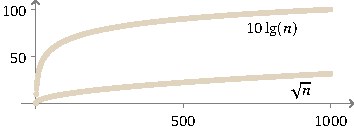
\includegraphics{complexity/asy/bigo/bigo00.pdf}
\end{center}
However,
in the long run the values of $\sqrt{x}$ are much larger than
the values of $10\lg(x)$.
For instance, $\sqrt{1\,000\,000}=1\,000$ while
$10\lg(1\,000\,000)\approx 199.32$.
\begin{center}
  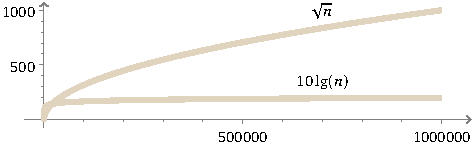
\includegraphics{complexity/asy/bigo/bigo01.pdf}
\end{center}

\margingraphic[l]{0.20\textwidth}{complexity/knuth.jpg}{\label{fig:knuth}\href{https://en.wikipedia.org/wiki/Donald_Knuth}{Donald Knuth b~1938 A pioneer of algorithm analysis}}
We can analyze the behavior of algorithms at length, finding exact algebraic expressions for how long they take, or how much memory, or how many disk reads, etc.
But for our purposes, 
we are usually interested in the long-term behavior of the function
on the large scale, as typified by the above graph,
We will therefore discount any initial chopping and changing.
Consonant with that, note that the factor of $10$ in $10\lg(x)$ is
unimportant; what matters is that a logarithm function~$10\ln(x)$ grows slower
than does a power function~$x^{1/2}$.
We will also take the view, in the definition below, that 
in choosing between two long term behaviors like the ones shown above,
we should discount constant factors.

\begin{example}
  
\end{example}




This definition reflects those considerations.

\begin{definition}
Let $\fcn{f,g}{\N}{\N}$.
Then \definend{$f$ is $\bigOh(g)$, written $f=\bigOh(g)$},
read ``$f$ is big-oh of $g$,''
when there are constants $N,C\in\N$ such that 
whenever $n>N$ then $f(n)<C\cdot g(n)$. 
\end{definition}

Think of `$f$ is $\bigOh(g)$' as meaning that
$f$'s growth rate is less than or equal to $g$'s rate.

\begin{remark}
The `$=$' notation is awkward but standard.
(sometimes written $f\in\bigOh(g)$), % or $f(n)=bigOh(g(n))$,
\end{remark}





\chapter{Computational resources}


\section{\textbf{NP}}
These two  
computational problems seem similar.

\begin{example}
Formally, a mathematical proof as a sequence of statements,
$\sigma_0$, $\sigma_1$, \ldots, $\sigma_k$,
where the final statement is the conclusion. 
Each statement either is itself an axiom or
else follows from the statements before it
by an application
of one of the agreed-upon derivation rules.
From experience we know that finding the proof of a desired  
conclusion can be very hard; often it seems to take a leap of insight.
Trying to brute-force it by taking all combinations of 
all the axioms and all the derivation rules would be very slow.
In contrast, if we were given the 
sequence of statements along with a description
of each step's rules, and asked only to check the 
sequence for correctness,
then that would be easy and quick.
\end{example}

\begin{example}
Consider a complicated propositional logic expression, say
$(\neg(P_1\vee (P_2\wedge P_3)\rightarrow \neg P_4)\leftrightarrow (P_2\rightarrow P_3)\rightarrow (P_1\wedge \neg P_4)$.
We want to find whether it is \definend{satisfiable}, 
whether there is any assignment of 
truth values $\true$ or~$\false$ to the 
variables $P_1,\idots, P_4$ that makes the statement
as a whole have the value $\true$.
We can imagine trying to answer by reasoning
in some way as, 
``Well, the formula has an if and only if arrow so I can see that
it boils down to \ldots''
but an algorithm that unfailingly finds the solution that way is not evident.
Alternatively, 
you could go through the possible assignments
$\seq{\false, \false, \false, \false}$, 
then $\seq{\false, \false, \false, \true}$, etc., 
until one causes the statement to yield $\true$, if one ever does.
However, if instead you were given an answer, an assignment to the variables,
and only asked to verify that it solves the problem, then you 
could do that quickly.
\end{example}

These seem alike in that, putting aside brute force,
we feel that for each finding an answer is hard and somehow involves creativity.
But if we are simply handed a solution then verifying that it is right 
calls only for a dull calculation.

That is, there are problems where finding an answer is quick and easy.
The two problems above seem different\Dash they \emph{feel} hard to solve, 
although
they have the property that once an answer is given then it is easy
to check.
Despite this very strong feeling, though, we are today unable
to prove that they are of different hardnesses.
This question of whether we can tell the two apart
is certainly the sexiest one in Computing today.
One reason it is attractive is that many pressing problems
have been shown to be like the proof-generating or satisfiability questions:
they don't appear to be solvable efficiently
their solutions can be verified quickly.
however, we cannot today prove that  
that is the case.  




\section{Complexity classes}
 
\begin{definition}[the complexity class $\compclass{NP}$]
A language $\lang{L}$ is a member of 
$\compclass{NP}$ if there is a polynomial $\map{p}{\N}{\N}$ and a
polynomial time Turing machine $\TM$, the \definend{verifier}
for $\lang{L}$, such that 
\begin{equation*}
  \forall \sigma\in\strings 
  \big[ \sigma\in\lang{L} 
     \,\Longleftrightarrow\, 
     \exists w\in \set{0,1}^{p(|\sigma|)}(\TM(\seq{\sigma,w})=1)  \big]
\end{equation*}
($w$ is the \definend{witness} or \definend{certificate} for $\sigma$).
\end{definition}

Note that the witness is restricted in length so that the verifier,
which as a Turing machine reads one bit at a time, can 
read it through in polynomial time.
Note also that we can take the polynomial~$p$ to be trivial $p(i)=0$
to get that $\compclass{P}\subseteq\compclass{NP}$.

\begin{exercises}
\begin{exercise}
In the definition of 
the complexity class $\compclass{NP}$, 
there is a different witness~$w$ for each~$\sigma$.
What if there is a single witness that works for all~$\sigma$?
\end{exercise}
\end{exercises}

% Use this as an example
% https://en.wikipedia.org/wiki/Belphegor%27s_prime

% Two algorithms, one is fast and one is slow
% http://blog.plover.com/2017/02/21/#anagram-scoring





% ===============================================================

\extra{Sudoku is $\compclass{NP}$ complete}





% \begin{figure}
% \oddpagelayoutfalse
% \twocolumnlayouttrue
% \pagediagram
% \caption{Left-hand two-column page layout parameters} \label{fig:pplt}
% \begin{center}
%   \pagevalues  
% \end{center}
% \end{figure}

\printnotes
\printbibliography
\end{document}
